\documentclass[twoside]{book}

% Packages required by doxygen
\usepackage{fixltx2e}
\usepackage{calc}
\usepackage{doxygen}
\usepackage[export]{adjustbox} % also loads graphicx
\usepackage{graphicx}
\usepackage[utf8]{inputenc}
\usepackage{makeidx}
\usepackage{multicol}
\usepackage{multirow}
\PassOptionsToPackage{warn}{textcomp}
\usepackage{textcomp}
\usepackage[nointegrals]{wasysym}
\usepackage[table]{xcolor}

% Font selection
\usepackage[T1]{fontenc}
\usepackage[scaled=.90]{helvet}
\usepackage{courier}
\usepackage{amssymb}
\usepackage{sectsty}
\renewcommand{\familydefault}{\sfdefault}
\allsectionsfont{%
  \fontseries{bc}\selectfont%
  \color{darkgray}%
}
\renewcommand{\DoxyLabelFont}{%
  \fontseries{bc}\selectfont%
  \color{darkgray}%
}
\newcommand{\+}{\discretionary{\mbox{\scriptsize$\hookleftarrow$}}{}{}}

% Page & text layout
\usepackage{geometry}
\geometry{%
  a4paper,%
  top=2.5cm,%
  bottom=2.5cm,%
  left=2.5cm,%
  right=2.5cm%
}
\tolerance=750
\hfuzz=15pt
\hbadness=750
\setlength{\emergencystretch}{15pt}
\setlength{\parindent}{0cm}
\setlength{\parskip}{3ex plus 2ex minus 2ex}
\makeatletter
\renewcommand{\paragraph}{%
  \@startsection{paragraph}{4}{0ex}{-1.0ex}{1.0ex}{%
    \normalfont\normalsize\bfseries\SS@parafont%
  }%
}
\renewcommand{\subparagraph}{%
  \@startsection{subparagraph}{5}{0ex}{-1.0ex}{1.0ex}{%
    \normalfont\normalsize\bfseries\SS@subparafont%
  }%
}
\makeatother

% Headers & footers
\usepackage{fancyhdr}
\pagestyle{fancyplain}
\fancyhead[LE]{\fancyplain{}{\bfseries\thepage}}
\fancyhead[CE]{\fancyplain{}{}}
\fancyhead[RE]{\fancyplain{}{\bfseries\leftmark}}
\fancyhead[LO]{\fancyplain{}{\bfseries\rightmark}}
\fancyhead[CO]{\fancyplain{}{}}
\fancyhead[RO]{\fancyplain{}{\bfseries\thepage}}
\fancyfoot[LE]{\fancyplain{}{}}
\fancyfoot[CE]{\fancyplain{}{}}
\fancyfoot[RE]{\fancyplain{}{\bfseries\scriptsize Generated by Doxygen }}
\fancyfoot[LO]{\fancyplain{}{\bfseries\scriptsize Generated by Doxygen }}
\fancyfoot[CO]{\fancyplain{}{}}
\fancyfoot[RO]{\fancyplain{}{}}
\renewcommand{\footrulewidth}{0.4pt}
\renewcommand{\chaptermark}[1]{%
  \markboth{#1}{}%
}
\renewcommand{\sectionmark}[1]{%
  \markright{\thesection\ #1}%
}

% Indices & bibliography
\usepackage{natbib}
\usepackage[titles]{tocloft}
\setcounter{tocdepth}{3}
\setcounter{secnumdepth}{5}
\makeindex

% Hyperlinks (required, but should be loaded last)
\usepackage{ifpdf}
\ifpdf
  \usepackage[pdftex,pagebackref=true]{hyperref}
\else
  \usepackage[ps2pdf,pagebackref=true]{hyperref}
\fi
\hypersetup{%
  colorlinks=true,%
  linkcolor=blue,%
  citecolor=blue,%
  unicode%
}

% Custom commands
\newcommand{\clearemptydoublepage}{%
  \newpage{\pagestyle{empty}\cleardoublepage}%
}

\usepackage{caption}
\captionsetup{labelsep=space,justification=centering,font={bf},singlelinecheck=off,skip=4pt,position=top}

%===== C O N T E N T S =====

\begin{document}

% Titlepage & ToC
\hypersetup{pageanchor=false,
             bookmarksnumbered=true,
             pdfencoding=unicode
            }
\pagenumbering{alph}
\begin{titlepage}
\vspace*{7cm}
\begin{center}%
{\Large Open\+Space\+Toolkit\+Astrodynamics \\[1ex]\large 0.\+9.\+3 }\\
\vspace*{1cm}
{\large Generated by Doxygen 1.8.13}\\
\end{center}
\end{titlepage}
\clearemptydoublepage
\pagenumbering{roman}
\tableofcontents
\clearemptydoublepage
\pagenumbering{arabic}
\hypersetup{pageanchor=true}

%--- Begin generated contents ---
\chapter{Open Space Toolkit ▸ Astrodynamics}
\label{index}\hypertarget{index}{}Structure\href{https://github.com/open-space-collective/open-space-toolkit-astrodynamics/actions/workflows/build-test.yml}{\texttt{ }} \href{https://codecov.io/gh/open-space-collective/open-space-toolkit-astrodynamics}{\texttt{ }} \href{https://open-space-collective.github.io/open-space-toolkit-astrodynamics}{\texttt{ }} \href{https://badge.fury.io/gh/open-space-collective\%2Fopen-space-toolkit-astrodynamics}{\texttt{ }} \href{https://badge.fury.io/py/open-space-toolkit-astrodynamics}{\texttt{ }} \href{https://opensource.org/licenses/Apache-2.0}{\texttt{ }}

Orbit, attitude, access.

\hypertarget{index_autotoc_md1}{}\doxysection{Getting Started}\label{index_autotoc_md1}
Want to get started? This is the simplest and quickest way\+:

\href{https://mybinder.org/v2/gh/open-space-collective/open-space-toolkit/main?urlpath=lab/tree/notebooks}{\texttt{ }}

{\itshape Nothing to download or install! This will automatically start a \href{https://jupyterlab.readthedocs.io/en/stable/}{\texttt{ Jupyter\+Lab}} environment in your browser with Open Space Toolkit libraries and example notebooks ready to use.}\hypertarget{index_autotoc_md2}{}\doxysubsection{Alternatives}\label{index_autotoc_md2}
\hypertarget{index_autotoc_md3}{}\doxysubsubsection{Docker Images}\label{index_autotoc_md3}
\href{https://www.docker.com/}{\texttt{ Docker}} must be installed on your system.\hypertarget{index_autotoc_md4}{}\doxyparagraph{i\+Python}\label{index_autotoc_md4}
The following command will start an \href{https://ipython.org/}{\texttt{ i\+Python}} shell within a container where the O\+S\+Tk components are already installed\+:


\begin{DoxyCode}{0}
\DoxyCodeLine{docker run -\/it openspacecollective/open-\/space-\/toolkit-\/astrodynamics-\/python}
\end{DoxyCode}


Once the shell is up and running, playing with it is easy\+:


\begin{DoxyCode}{0}
\DoxyCodeLine{\textcolor{keyword}{from} ostk.physics \textcolor{keyword}{import} Environment}
\DoxyCodeLine{\textcolor{keyword}{from} ostk.physics.time \textcolor{keyword}{import} Instant}
\DoxyCodeLine{\textcolor{keyword}{from} ostk.astrodynamics.trajectory \textcolor{keyword}{import} Orbit}
\DoxyCodeLine{\textcolor{keyword}{from} ostk.astrodynamics.trajectory.orbit.models \textcolor{keyword}{import} SGP4}
\DoxyCodeLine{\textcolor{keyword}{from} ostk.astrodynamics.trajectory.orbit.models.sgp4 \textcolor{keyword}{import} TLE}
\DoxyCodeLine{}
\DoxyCodeLine{tle = TLE(}
\DoxyCodeLine{    \textcolor{stringliteral}{'1 25544U 98067A   18231.17878740  .00000187  00000-\/0  10196-\/4 0  9994'},}
\DoxyCodeLine{    \textcolor{stringliteral}{'2 25544  51.6447  64.7824 0005971  73.1467  36.4366 15.53848234128316'}}
\DoxyCodeLine{)  \textcolor{comment}{\# Construct Two-\/Line Element set}}
\DoxyCodeLine{}
\DoxyCodeLine{earth = Environment.default().access\_celestial\_object\_with\_name(\textcolor{stringliteral}{'Earth'})  \textcolor{comment}{\# Access Earth model}}
\DoxyCodeLine{}
\DoxyCodeLine{orbit = Orbit(SGP4(tle), earth)  \textcolor{comment}{\# Construct orbit using SGP4 model}}
\DoxyCodeLine{}
\DoxyCodeLine{orbit.get\_state\_at(Instant.now())  \textcolor{comment}{\# Compute and display current satellite state (position, velocity)}}
\end{DoxyCode}


By default, O\+S\+Tk fetches the ephemeris from J\+PL, Earth Orientation Parameters (E\+OP) and leap second count from I\+E\+RS.

As a result, when running O\+S\+Tk for the first time, it may take a minute to fetch all the necessary data.

{\itshape Tip\+: Use tab for auto-\/completion!}\hypertarget{index_autotoc_md5}{}\doxyparagraph{Jupyter\+Lab}\label{index_autotoc_md5}
The following command will start a \href{https://jupyterlab.readthedocs.io/en/stable/}{\texttt{ Jupyter\+Lab}} server within a container where the O\+S\+Tk components are already installed\+:


\begin{DoxyCode}{0}
\DoxyCodeLine{docker run -\/-\/publish=8888:8888 openspacecollective/open-\/space-\/toolkit-\/astrodynamics-\/jupyter}
\end{DoxyCode}


Once the container is running, access \href{http://localhost:8888/lab}{\texttt{ http\+://localhost\+:8888/lab}} and create a Python 3 Notebook.\hypertarget{index_autotoc_md6}{}\doxysection{Installation}\label{index_autotoc_md6}
\hypertarget{index_autotoc_md7}{}\doxysubsection{C++}\label{index_autotoc_md7}
The binary packages are hosted using \href{https://github.com/open-space-collective/open-space-toolkit-astrodynamics/releases}{\texttt{ Git\+Hub Releases}}\+:


\begin{DoxyItemize}
\item Runtime libraries\+: {\ttfamily open-\/space-\/toolkit-\/astrodynamics-\/\+X.\+Y.\+Z-\/1.\+x86\+\_\+64-\/runtime}
\item C++ headers\+: {\ttfamily open-\/space-\/toolkit-\/astrodynamics-\/\+X.\+Y.\+Z-\/1.\+x86\+\_\+64-\/devel}
\item Python bindings\+: {\ttfamily open-\/space-\/toolkit-\/astrodynamics-\/\+X.\+Y.\+Z-\/1.\+x86\+\_\+64-\/python}
\end{DoxyItemize}\hypertarget{index_autotoc_md8}{}\doxysubsubsection{Debian / Ubuntu}\label{index_autotoc_md8}
After downloading the relevant {\ttfamily .deb} binary packages, install\+:


\begin{DoxyCode}{0}
\DoxyCodeLine{apt install open-\/space-\/toolkit-\/astrodynamics-\/*.deb}
\end{DoxyCode}
\hypertarget{index_autotoc_md9}{}\doxysubsection{Python}\label{index_autotoc_md9}
Install from \href{https://pypi.org/project/open-space-toolkit-astrodynamics/}{\texttt{ Py\+PI}}\+:


\begin{DoxyCode}{0}
\DoxyCodeLine{pip install open-\/space-\/toolkit-\/astrodynamics}
\end{DoxyCode}
\hypertarget{index_autotoc_md10}{}\doxysection{Documentation}\label{index_autotoc_md10}
Documentation is available here\+:


\begin{DoxyItemize}
\item \href{https://open-space-collective.github.io/open-space-toolkit-astrodynamics}{\texttt{ C++}}
\item \href{./bindings/python/docs}{\texttt{ Python}}
\end{DoxyItemize}

$<$details$>$

The library exhibits the following detailed and descriptive structure\+:


\begin{DoxyCode}{0}
\DoxyCodeLine{├── NumericalSolver}
\DoxyCodeLine{├── Trajectory}
\DoxyCodeLine{│   ├── State}
\DoxyCodeLine{│   ├── Orbit}
\DoxyCodeLine{│   │   ├── Models}
\DoxyCodeLine{│   │   │   ├── Kepler}
\DoxyCodeLine{│   │   │   │   └── Classical Orbital Elements (COE)}
\DoxyCodeLine{│   │   │   ├── SGP4}
\DoxyCodeLine{│   │   │   │   └── Two-\/Line Element set (TLE)}
\DoxyCodeLine{│   │   │   ├── Tabulated (input csv)}
\DoxyCodeLine{│   │   │   └── Propagated (numerical integration)}
\DoxyCodeLine{│   │   ├── Pass}
\DoxyCodeLine{|   |   └── Messages}
\DoxyCodeLine{|   |       └── SpaceX}
\DoxyCodeLine{|   |           └── OPM}
\DoxyCodeLine{│   ├── Models}
\DoxyCodeLine{│   |   ├── Static}
\DoxyCodeLine{│   |   └── Tabulated}
\DoxyCodeLine{│   └── Propagator}
\DoxyCodeLine{├── Flight}
\DoxyCodeLine{│   ├── Profile}
\DoxyCodeLine{|   |    ├── Models}
\DoxyCodeLine{│   |    |   ├── Transform}
\DoxyCodeLine{│   |    |   └── Tabulated}
\DoxyCodeLine{│   |    └── State}
\DoxyCodeLine{│   └── System}
\DoxyCodeLine{|        ├── SatelliteSystem}
\DoxyCodeLine{|        └── Dynamics}
\DoxyCodeLine{|            └── SatelliteDynamics}
\DoxyCodeLine{├── Access}
\DoxyCodeLine{|   └── Generator}
\DoxyCodeLine{└── Conjunction}
\DoxyCodeLine{    └── Messages}
\DoxyCodeLine{        └── CCSDS}
\DoxyCodeLine{            └── CDM}
\end{DoxyCode}


$<$/details$>$\hypertarget{index_autotoc_md11}{}\doxysection{Tutorials}\label{index_autotoc_md11}
Tutorials are available here\+:


\begin{DoxyItemize}
\item \href{./tutorials/cpp}{\texttt{ C++}}
\item \href{./tutorials/python}{\texttt{ Python}}
\end{DoxyItemize}\hypertarget{index_autotoc_md12}{}\doxysection{Setup}\label{index_autotoc_md12}
\hypertarget{index_autotoc_md13}{}\doxysubsection{Development Environment}\label{index_autotoc_md13}
Using \href{https://www.docker.com}{\texttt{ Docker}} for development is recommended, to simplify the installation of the necessary build tools and dependencies. Instructions on how to install Docker are available \href{https://docs.docker.com/install/}{\texttt{ here}}.

To start the development environment\+:


\begin{DoxyCode}{0}
\DoxyCodeLine{make start-\/development}
\end{DoxyCode}


This will\+:


\begin{DoxyEnumerate}
\item Build the {\ttfamily openspacecollective/open-\/space-\/toolkit-\/astrodynamics-\/development} Docker image.
\item Create a development environment container with local source files and helper scripts mounted.
\item Start a {\ttfamily bash} shell from the {\ttfamily ./build} working directory.
\end{DoxyEnumerate}

If installing Docker is not an option, you can manually install the development tools (G\+CC, C\+Make) and all required dependencies, by following a procedure similar to the one described in the \href{./docker/development/Dockerfile}{\texttt{ Development Dockerfile}}.\hypertarget{index_autotoc_md14}{}\doxysubsection{Build}\label{index_autotoc_md14}
From the {\ttfamily ./build} directory\+:


\begin{DoxyCode}{0}
\DoxyCodeLine{cmake ..}
\DoxyCodeLine{make}
\end{DoxyCode}


{\itshape Tip\+: {\ttfamily helpers/build.\+sh} simplifies building from within the development environment.}\hypertarget{index_autotoc_md15}{}\doxysubsection{Test}\label{index_autotoc_md15}
To start a container to build and run the tests\+:


\begin{DoxyCode}{0}
\DoxyCodeLine{make test}
\end{DoxyCode}


Or to run them manually\+:


\begin{DoxyCode}{0}
\DoxyCodeLine{./bin/open-\/space-\/toolkit-\/astrodynamics.test}
\end{DoxyCode}


{\itshape Tip\+: {\ttfamily helpers/test.\+sh} simplifies running tests from within the development environment.}\hypertarget{index_autotoc_md16}{}\doxysection{Dependencies}\label{index_autotoc_md16}
\tabulinesep=1mm
\begin{longtabu}spread 0pt [c]{*{4}{|X[-1]}|}
\hline
\PBS\centering \cellcolor{\tableheadbgcolor}\textbf{ Name }&\PBS\centering \cellcolor{\tableheadbgcolor}\textbf{ Version }&\PBS\centering \cellcolor{\tableheadbgcolor}\textbf{ License }&\PBS\centering \cellcolor{\tableheadbgcolor}\textbf{ Link  }\\\cline{1-4}
\endfirsthead
\hline
\endfoot
\hline
\PBS\centering \cellcolor{\tableheadbgcolor}\textbf{ Name }&\PBS\centering \cellcolor{\tableheadbgcolor}\textbf{ Version }&\PBS\centering \cellcolor{\tableheadbgcolor}\textbf{ License }&\PBS\centering \cellcolor{\tableheadbgcolor}\textbf{ Link  }\\\cline{1-4}
\endhead
Pybind11 &{\ttfamily 2.\+10.\+1} &B\+S\+D-\/3-\/\+Clause &\href{https://github.com/pybind/pybind11}{\texttt{ github.\+com/pybind/pybind11}}  \\\cline{1-4}
ordered-\/map &{\ttfamily 0.\+6.\+0} &M\+IT &\href{https://github.com/Tessil/ordered-map}{\texttt{ github.\+com/\+Tessil/ordered-\/map}}  \\\cline{1-4}
Eigen &{\ttfamily 3.\+3.\+7} &M\+P\+L2 &\href{http://eigen.tuxfamily.org/index.php}{\texttt{ eigen.\+tuxfamily.\+org}}  \\\cline{1-4}
S\+G\+P4 &{\ttfamily 6a448b4} &Apache License 2.\+0 &\href{https://github.com/dnwrnr/sgp4}{\texttt{ github.\+com/dnwrnr/sgp4}}  \\\cline{1-4}
N\+Lopt &{\ttfamily 2.\+5.\+0} &L\+G\+PL &\href{https://github.com/stevengj/nlopt}{\texttt{ github.\+com/stevengj/nlopt}}  \\\cline{1-4}
Core &{\ttfamily main} &Apache License 2.\+0 &\href{https://github.com/open-space-collective/open-space-toolkit-core}{\texttt{ github.\+com/open-\/space-\/collective/open-\/space-\/toolkit-\/core}}  \\\cline{1-4}
I/O &{\ttfamily main} &Apache License 2.\+0 &\href{https://github.com/open-space-collective/open-space-toolkit-io}{\texttt{ github.\+com/open-\/space-\/collective/open-\/space-\/toolkit-\/io}}  \\\cline{1-4}
Mathematics &{\ttfamily main} &Apache License 2.\+0 &\href{https://github.com/open-space-collective/open-space-toolkit-mathematics}{\texttt{ github.\+com/open-\/space-\/collective/open-\/space-\/toolkit-\/mathematics}}  \\\cline{1-4}
Physics &{\ttfamily main} &Apache License 2.\+0 &\href{https://github.com/open-space-collective/open-space-toolkit-physics}{\texttt{ github.\+com/open-\/space-\/collective/open-\/space-\/toolkit-\/physics}}  \\\cline{1-4}
\end{longtabu}
\hypertarget{index_autotoc_md17}{}\doxysection{Contribution}\label{index_autotoc_md17}
Contributions are more than welcome!

Please read our \mbox{\hyperlink{_c_o_n_t_r_i_b_u_t_i_n_g_8md}{contributing guide}} to learn about our development process, how to propose fixes and improvements, and how to build and test the code.\hypertarget{index_autotoc_md18}{}\doxysection{Special Thanks}\label{index_autotoc_md18}
\href{https://www.loftorbital.com/}{\texttt{ }}\hypertarget{index_autotoc_md19}{}\doxysection{License}\label{index_autotoc_md19}
Apache License 2.\+0 
\chapter{Contributing}
\label{md__c_o_n_t_r_i_b_u_t_i_n_g}
\Hypertarget{md__c_o_n_t_r_i_b_u_t_i_n_g}
{\itshape ⚠ This document is a work in progress.}\hypertarget{md__c_o_n_t_r_i_b_u_t_i_n_g_Introduction}{}\doxysection{Introduction}\label{md__c_o_n_t_r_i_b_u_t_i_n_g_Introduction}
{\itshape To be completed...}\hypertarget{md__c_o_n_t_r_i_b_u_t_i_n_g_Guidelines}{}\doxysection{Guidelines}\label{md__c_o_n_t_r_i_b_u_t_i_n_g_Guidelines}
\hypertarget{md__c_o_n_t_r_i_b_u_t_i_n_g_Codebase}{}\doxysubsection{Codebase}\label{md__c_o_n_t_r_i_b_u_t_i_n_g_Codebase}
\hypertarget{md__c_o_n_t_r_i_b_u_t_i_n_g_C}{}\doxysubsubsection{C++}\label{md__c_o_n_t_r_i_b_u_t_i_n_g_C}
Include order from specific to generic\+:


\begin{DoxyCode}{0}
\DoxyCodeLine{\textcolor{preprocessor}{\#include <OpenSpaceToolkit/Astrodynamics/Orbit.hpp>}}
\DoxyCodeLine{}
\DoxyCodeLine{\textcolor{preprocessor}{\#include <OpenSpaceToolkit/Core/Types/Integer.hpp>}}
\DoxyCodeLine{\textcolor{preprocessor}{\#include <OpenSpaceToolkit/Core/Utilities.hpp>}}
\DoxyCodeLine{}
\DoxyCodeLine{\textcolor{preprocessor}{\#include <map>}}
\DoxyCodeLine{\textcolor{preprocessor}{\#include <string>}}
\end{DoxyCode}


References\+:


\begin{DoxyItemize}
\item \href{https://stackoverflow.com/questions/2762568/c-c-include-file-order-best-practices}{\texttt{ https\+://stackoverflow.\+com/questions/2762568/c-\/c-\/include-\/file-\/order-\/best-\/practices}}
\item \href{https://blog.kowalczyk.info/article/qg/order-of-include-headers-in-cc.html}{\texttt{ https\+://blog.\+kowalczyk.\+info/article/qg/order-\/of-\/include-\/headers-\/in-\/cc.\+html}}
\end{DoxyItemize}\hypertarget{md__c_o_n_t_r_i_b_u_t_i_n_g_Python}{}\doxysubsubsection{Python}\label{md__c_o_n_t_r_i_b_u_t_i_n_g_Python}
{\itshape To be completed...}\hypertarget{md__c_o_n_t_r_i_b_u_t_i_n_g_Version}{}\doxysubsection{Version Control}\label{md__c_o_n_t_r_i_b_u_t_i_n_g_Version}
\hypertarget{md__c_o_n_t_r_i_b_u_t_i_n_g_Rules}{}\doxysubsubsection{Rules}\label{md__c_o_n_t_r_i_b_u_t_i_n_g_Rules}
{\itshape To be completed...}\hypertarget{md__c_o_n_t_r_i_b_u_t_i_n_g_Commit}{}\doxysubsubsection{Commit Messages}\label{md__c_o_n_t_r_i_b_u_t_i_n_g_Commit}
\href{https://chris.beams.io/posts/git-commit/}{\texttt{ How to Write a Git Commit Message}}

Use active form ({\ttfamily Do something}).

Prefix commit messages using the following tags\+:


\begin{DoxyItemize}
\item \mbox{[}feature\mbox{]}
\item \mbox{[}fix\mbox{]}
\item \mbox{[}misc\mbox{]}
\end{DoxyItemize}

Examples\+:


\begin{DoxyCode}{0}
\DoxyCodeLine{[feature] Implement high fidelity orbit propagator}
\end{DoxyCode}



\begin{DoxyCode}{0}
\DoxyCodeLine{[fix] Segmentation fault when fetching ephemeris data}
\end{DoxyCode}
\hypertarget{md__c_o_n_t_r_i_b_u_t_i_n_g_CodeOfConduct}{}\doxysection{Code of Conduct}\label{md__c_o_n_t_r_i_b_u_t_i_n_g_CodeOfConduct}
{\itshape To be completed...} 
\chapter{Tutorial}
\label{md_docs__tutorial}
\Hypertarget{md_docs__tutorial}
Below are examples illustrating a few common use-\/cases.\hypertarget{md_docs__tutorial_Setup}{}\doxysection{Setup}\label{md_docs__tutorial_Setup}
{\itshape To be completed...}\hypertarget{md_docs__tutorial_Examples}{}\doxysection{Examples}\label{md_docs__tutorial_Examples}
{\itshape To be completed...} 
\chapter{Namespace Index}
\doxysection{Namespace List}
Here is a list of all namespaces with brief descriptions\+:\begin{DoxyCompactList}
\item\contentsline{section}{\mbox{\hyperlink{namespaceostk}{ostk}} \\*Apache License 2.\+0 }{\pageref{namespaceostk}}{}
\item\contentsline{section}{\mbox{\hyperlink{namespaceostk_1_1astro}{ostk\+::astro}} }{\pageref{namespaceostk_1_1astro}}{}
\item\contentsline{section}{\mbox{\hyperlink{namespaceostk_1_1astro_1_1access}{ostk\+::astro\+::access}} }{\pageref{namespaceostk_1_1astro_1_1access}}{}
\item\contentsline{section}{\mbox{\hyperlink{namespaceostk_1_1astro_1_1conjunction}{ostk\+::astro\+::conjunction}} }{\pageref{namespaceostk_1_1astro_1_1conjunction}}{}
\item\contentsline{section}{\mbox{\hyperlink{namespaceostk_1_1astro_1_1conjunction_1_1messages}{ostk\+::astro\+::conjunction\+::messages}} }{\pageref{namespaceostk_1_1astro_1_1conjunction_1_1messages}}{}
\item\contentsline{section}{\mbox{\hyperlink{namespaceostk_1_1astro_1_1conjunction_1_1messages_1_1ccsds}{ostk\+::astro\+::conjunction\+::messages\+::ccsds}} }{\pageref{namespaceostk_1_1astro_1_1conjunction_1_1messages_1_1ccsds}}{}
\item\contentsline{section}{\mbox{\hyperlink{namespaceostk_1_1astro_1_1eventcondition}{ostk\+::astro\+::eventcondition}} }{\pageref{namespaceostk_1_1astro_1_1eventcondition}}{}
\item\contentsline{section}{\mbox{\hyperlink{namespaceostk_1_1astro_1_1flight}{ostk\+::astro\+::flight}} }{\pageref{namespaceostk_1_1astro_1_1flight}}{}
\item\contentsline{section}{\mbox{\hyperlink{namespaceostk_1_1astro_1_1flight_1_1profile}{ostk\+::astro\+::flight\+::profile}} }{\pageref{namespaceostk_1_1astro_1_1flight_1_1profile}}{}
\item\contentsline{section}{\mbox{\hyperlink{namespaceostk_1_1astro_1_1flight_1_1profile_1_1models}{ostk\+::astro\+::flight\+::profile\+::models}} }{\pageref{namespaceostk_1_1astro_1_1flight_1_1profile_1_1models}}{}
\item\contentsline{section}{\mbox{\hyperlink{namespaceostk_1_1astro_1_1flight_1_1system}{ostk\+::astro\+::flight\+::system}} }{\pageref{namespaceostk_1_1astro_1_1flight_1_1system}}{}
\item\contentsline{section}{\mbox{\hyperlink{namespaceostk_1_1astro_1_1flight_1_1system_1_1dynamics}{ostk\+::astro\+::flight\+::system\+::dynamics}} }{\pageref{namespaceostk_1_1astro_1_1flight_1_1system_1_1dynamics}}{}
\item\contentsline{section}{\mbox{\hyperlink{namespaceostk_1_1astro_1_1flight_1_1system_1_1dynamics_1_1thruster}{ostk\+::astro\+::flight\+::system\+::dynamics\+::thruster}} }{\pageref{namespaceostk_1_1astro_1_1flight_1_1system_1_1dynamics_1_1thruster}}{}
\item\contentsline{section}{\mbox{\hyperlink{namespaceostk_1_1astro_1_1solvers}{ostk\+::astro\+::solvers}} }{\pageref{namespaceostk_1_1astro_1_1solvers}}{}
\item\contentsline{section}{\mbox{\hyperlink{namespaceostk_1_1astro_1_1trajectory}{ostk\+::astro\+::trajectory}} }{\pageref{namespaceostk_1_1astro_1_1trajectory}}{}
\item\contentsline{section}{\mbox{\hyperlink{namespaceostk_1_1astro_1_1trajectory_1_1models}{ostk\+::astro\+::trajectory\+::models}} }{\pageref{namespaceostk_1_1astro_1_1trajectory_1_1models}}{}
\item\contentsline{section}{\mbox{\hyperlink{namespaceostk_1_1astro_1_1trajectory_1_1orbit}{ostk\+::astro\+::trajectory\+::orbit}} }{\pageref{namespaceostk_1_1astro_1_1trajectory_1_1orbit}}{}
\item\contentsline{section}{\mbox{\hyperlink{namespaceostk_1_1astro_1_1trajectory_1_1orbit_1_1messages}{ostk\+::astro\+::trajectory\+::orbit\+::messages}} }{\pageref{namespaceostk_1_1astro_1_1trajectory_1_1orbit_1_1messages}}{}
\item\contentsline{section}{\mbox{\hyperlink{namespaceostk_1_1astro_1_1trajectory_1_1orbit_1_1messages_1_1spacex}{ostk\+::astro\+::trajectory\+::orbit\+::messages\+::spacex}} }{\pageref{namespaceostk_1_1astro_1_1trajectory_1_1orbit_1_1messages_1_1spacex}}{}
\item\contentsline{section}{\mbox{\hyperlink{namespaceostk_1_1astro_1_1trajectory_1_1orbit_1_1models}{ostk\+::astro\+::trajectory\+::orbit\+::models}} }{\pageref{namespaceostk_1_1astro_1_1trajectory_1_1orbit_1_1models}}{}
\item\contentsline{section}{\mbox{\hyperlink{namespaceostk_1_1astro_1_1trajectory_1_1orbit_1_1models_1_1kepler}{ostk\+::astro\+::trajectory\+::orbit\+::models\+::kepler}} }{\pageref{namespaceostk_1_1astro_1_1trajectory_1_1orbit_1_1models_1_1kepler}}{}
\item\contentsline{section}{\mbox{\hyperlink{namespaceostk_1_1astro_1_1trajectory_1_1orbit_1_1models_1_1sgp4}{ostk\+::astro\+::trajectory\+::orbit\+::models\+::sgp4}} }{\pageref{namespaceostk_1_1astro_1_1trajectory_1_1orbit_1_1models_1_1sgp4}}{}
\item\contentsline{section}{\mbox{\hyperlink{namespaceostk_1_1astro_1_1trajectory_1_1state}{ostk\+::astro\+::trajectory\+::state}} }{\pageref{namespaceostk_1_1astro_1_1trajectory_1_1state}}{}
\item\contentsline{section}{\mbox{\hyperlink{namespaceostk_1_1astro_1_1trajectory_1_1state_1_1coordinatessubsets}{ostk\+::astro\+::trajectory\+::state\+::coordinatessubsets}} }{\pageref{namespaceostk_1_1astro_1_1trajectory_1_1state_1_1coordinatessubsets}}{}
\end{DoxyCompactList}

\chapter{Hierarchical Index}
\doxysection{Class Hierarchy}
This inheritance list is sorted roughly, but not completely, alphabetically\+:\begin{DoxyCompactList}
\item \contentsline{section}{ostk\+::astro\+::Access}{\pageref{classostk_1_1astro_1_1_access}}{}
\item \contentsline{section}{ostk\+::astro\+::conjunction\+::messages\+::ccsds\+::C\+DM}{\pageref{classostk_1_1astro_1_1conjunction_1_1messages_1_1ccsds_1_1_c_d_m}}{}
\item \contentsline{section}{ostk\+::astro\+::trajectory\+::orbit\+::models\+::kepler\+::C\+OE}{\pageref{classostk_1_1astro_1_1trajectory_1_1orbit_1_1models_1_1kepler_1_1_c_o_e}}{}
\item \contentsline{section}{ostk\+::astro\+::Numerical\+Solver\+::Condition\+Solution}{\pageref{structostk_1_1astro_1_1_numerical_solver_1_1_condition_solution}}{}
\item \contentsline{section}{ostk\+::astro\+::trajectory\+::state\+::Coordinates\+Broker}{\pageref{classostk_1_1astro_1_1trajectory_1_1state_1_1_coordinates_broker}}{}
\item \contentsline{section}{ostk\+::astro\+::trajectory\+::state\+::Coordinates\+Subset}{\pageref{classostk_1_1astro_1_1trajectory_1_1state_1_1_coordinates_subset}}{}
\begin{DoxyCompactList}
\item \contentsline{section}{ostk\+::astro\+::trajectory\+::state\+::coordinatessubsets\+::Cartesian\+Position}{\pageref{classostk_1_1astro_1_1trajectory_1_1state_1_1coordinatessubsets_1_1_cartesian_position}}{}
\item \contentsline{section}{ostk\+::astro\+::trajectory\+::state\+::coordinatessubsets\+::Cartesian\+Velocity}{\pageref{classostk_1_1astro_1_1trajectory_1_1state_1_1coordinatessubsets_1_1_cartesian_velocity}}{}
\end{DoxyCompactList}
\item \contentsline{section}{ostk\+::astro\+::conjunction\+::messages\+::ccsds\+::C\+DM\+::Data}{\pageref{structostk_1_1astro_1_1conjunction_1_1messages_1_1ccsds_1_1_c_d_m_1_1_data}}{}
\item \contentsline{section}{ostk\+::astro\+::trajectory\+::orbit\+::messages\+::spacex\+::O\+PM\+::Deployment}{\pageref{structostk_1_1astro_1_1trajectory_1_1orbit_1_1messages_1_1spacex_1_1_o_p_m_1_1_deployment}}{}
\item \contentsline{section}{ostk\+::astro\+::flight\+::system\+::Dynamics}{\pageref{classostk_1_1astro_1_1flight_1_1system_1_1_dynamics}}{}
\begin{DoxyCompactList}
\item \contentsline{section}{ostk\+::astro\+::flight\+::system\+::dynamics\+::Atmospheric\+Drag}{\pageref{classostk_1_1astro_1_1flight_1_1system_1_1dynamics_1_1_atmospheric_drag}}{}
\item \contentsline{section}{ostk\+::astro\+::flight\+::system\+::dynamics\+::Central\+Body\+Gravity}{\pageref{classostk_1_1astro_1_1flight_1_1system_1_1dynamics_1_1_central_body_gravity}}{}
\item \contentsline{section}{ostk\+::astro\+::flight\+::system\+::dynamics\+::Position\+Derivative}{\pageref{classostk_1_1astro_1_1flight_1_1system_1_1dynamics_1_1_position_derivative}}{}
\item \contentsline{section}{ostk\+::astro\+::flight\+::system\+::dynamics\+::Third\+Body\+Gravity}{\pageref{classostk_1_1astro_1_1flight_1_1system_1_1dynamics_1_1_third_body_gravity}}{}
\end{DoxyCompactList}
\item \contentsline{section}{ostk\+::astro\+::Event\+Condition}{\pageref{classostk_1_1astro_1_1_event_condition}}{}
\begin{DoxyCompactList}
\item \contentsline{section}{ostk\+::astro\+::eventcondition\+::C\+O\+E\+Condition}{\pageref{classostk_1_1astro_1_1eventcondition_1_1_c_o_e_condition}}{}
\item \contentsline{section}{ostk\+::astro\+::eventcondition\+::Duration\+Condition}{\pageref{classostk_1_1astro_1_1eventcondition_1_1_duration_condition}}{}
\item \contentsline{section}{ostk\+::astro\+::eventcondition\+::Logical\+Connective}{\pageref{classostk_1_1astro_1_1eventcondition_1_1_logical_connective}}{}
\begin{DoxyCompactList}
\item \contentsline{section}{ostk\+::astro\+::eventcondition\+::Conjunctive}{\pageref{classostk_1_1astro_1_1eventcondition_1_1_conjunctive}}{}
\item \contentsline{section}{ostk\+::astro\+::eventcondition\+::Disjunctive}{\pageref{classostk_1_1astro_1_1eventcondition_1_1_disjunctive}}{}
\end{DoxyCompactList}
\end{DoxyCompactList}
\item \contentsline{section}{ostk\+::astro\+::access\+::Generator}{\pageref{classostk_1_1astro_1_1access_1_1_generator}}{}
\item \contentsline{section}{ostk\+::astro\+::access\+::Generator\+Context}{\pageref{classostk_1_1astro_1_1access_1_1_generator_context}}{}
\item \contentsline{section}{ostk\+::astro\+::conjunction\+::messages\+::ccsds\+::C\+DM\+::Header}{\pageref{structostk_1_1astro_1_1conjunction_1_1messages_1_1ccsds_1_1_c_d_m_1_1_header}}{}
\item \contentsline{section}{ostk\+::astro\+::trajectory\+::orbit\+::messages\+::spacex\+::O\+PM\+::Header}{\pageref{structostk_1_1astro_1_1trajectory_1_1orbit_1_1messages_1_1spacex_1_1_o_p_m_1_1_header}}{}
\item \contentsline{section}{ostk\+::astro\+::conjunction\+::messages\+::ccsds\+::C\+DM\+::Metadata}{\pageref{structostk_1_1astro_1_1conjunction_1_1messages_1_1ccsds_1_1_c_d_m_1_1_metadata}}{}
\item \contentsline{section}{ostk\+::astro\+::trajectory\+::Model}{\pageref{classostk_1_1astro_1_1trajectory_1_1_model}}{}
\begin{DoxyCompactList}
\item \contentsline{section}{ostk\+::astro\+::trajectory\+::models\+::Static}{\pageref{classostk_1_1astro_1_1trajectory_1_1models_1_1_static}}{}
\item \contentsline{section}{ostk\+::astro\+::trajectory\+::models\+::Tabulated}{\pageref{classostk_1_1astro_1_1trajectory_1_1models_1_1_tabulated}}{}
\begin{DoxyCompactList}
\item \contentsline{section}{ostk\+::astro\+::trajectory\+::orbit\+::models\+::Tabulated}{\pageref{classostk_1_1astro_1_1trajectory_1_1orbit_1_1models_1_1_tabulated}}{}
\end{DoxyCompactList}
\item \contentsline{section}{ostk\+::astro\+::trajectory\+::orbit\+::Model}{\pageref{classostk_1_1astro_1_1trajectory_1_1orbit_1_1_model}}{}
\begin{DoxyCompactList}
\item \contentsline{section}{ostk\+::astro\+::trajectory\+::orbit\+::models\+::Kepler}{\pageref{classostk_1_1astro_1_1trajectory_1_1orbit_1_1models_1_1_kepler}}{}
\item \contentsline{section}{ostk\+::astro\+::trajectory\+::orbit\+::models\+::Propagated}{\pageref{classostk_1_1astro_1_1trajectory_1_1orbit_1_1models_1_1_propagated}}{}
\item \contentsline{section}{ostk\+::astro\+::trajectory\+::orbit\+::models\+::S\+G\+P4}{\pageref{classostk_1_1astro_1_1trajectory_1_1orbit_1_1models_1_1_s_g_p4}}{}
\item \contentsline{section}{ostk\+::astro\+::trajectory\+::orbit\+::models\+::Tabulated}{\pageref{classostk_1_1astro_1_1trajectory_1_1orbit_1_1models_1_1_tabulated}}{}
\end{DoxyCompactList}
\end{DoxyCompactList}
\item \contentsline{section}{ostk\+::astro\+::flight\+::profile\+::Model}{\pageref{classostk_1_1astro_1_1flight_1_1profile_1_1_model}}{}
\begin{DoxyCompactList}
\item \contentsline{section}{ostk\+::astro\+::flight\+::profile\+::models\+::Tabulated}{\pageref{classostk_1_1astro_1_1flight_1_1profile_1_1models_1_1_tabulated}}{}
\item \contentsline{section}{ostk\+::astro\+::flight\+::profile\+::models\+::Transform}{\pageref{classostk_1_1astro_1_1flight_1_1profile_1_1models_1_1_transform}}{}
\end{DoxyCompactList}
\item \contentsline{section}{ostk\+::astro\+::Numerical\+Solver}{\pageref{classostk_1_1astro_1_1_numerical_solver}}{}
\item \contentsline{section}{ostk\+::astro\+::trajectory\+::orbit\+::messages\+::spacex\+::O\+PM}{\pageref{classostk_1_1astro_1_1trajectory_1_1orbit_1_1messages_1_1spacex_1_1_o_p_m}}{}
\item \contentsline{section}{ostk\+::astro\+::trajectory\+::orbit\+::Pass}{\pageref{classostk_1_1astro_1_1trajectory_1_1orbit_1_1_pass}}{}
\item \contentsline{section}{ostk\+::astro\+::flight\+::Profile}{\pageref{classostk_1_1astro_1_1flight_1_1_profile}}{}
\item \contentsline{section}{ostk\+::astro\+::trajectory\+::Propagator}{\pageref{classostk_1_1astro_1_1trajectory_1_1_propagator}}{}
\item \contentsline{section}{ostk\+::astro\+::conjunction\+::messages\+::ccsds\+::C\+DM\+::Relative\+Metadata}{\pageref{structostk_1_1astro_1_1conjunction_1_1messages_1_1ccsds_1_1_c_d_m_1_1_relative_metadata}}{}
\item \contentsline{section}{ostk\+::astro\+::Root\+Solver}{\pageref{classostk_1_1astro_1_1_root_solver}}{}
\item \contentsline{section}{ostk\+::astro\+::Root\+Solver\+::Solution}{\pageref{structostk_1_1astro_1_1_root_solver_1_1_solution}}{}
\item \contentsline{section}{ostk\+::astro\+::trajectory\+::State}{\pageref{classostk_1_1astro_1_1trajectory_1_1_state}}{}
\item \contentsline{section}{ostk\+::astro\+::flight\+::profile\+::State}{\pageref{classostk_1_1astro_1_1flight_1_1profile_1_1_state}}{}
\item \contentsline{section}{ostk\+::astro\+::flight\+::System}{\pageref{classostk_1_1astro_1_1flight_1_1_system}}{}
\begin{DoxyCompactList}
\item \contentsline{section}{ostk\+::astro\+::flight\+::system\+::Satellite\+System}{\pageref{classostk_1_1astro_1_1flight_1_1system_1_1_satellite_system}}{}
\end{DoxyCompactList}
\item \contentsline{section}{ostk\+::astro\+::solvers\+::Temporal\+Condition\+Solver}{\pageref{classostk_1_1astro_1_1solvers_1_1_temporal_condition_solver}}{}
\item \contentsline{section}{ostk\+::astro\+::trajectory\+::orbit\+::models\+::sgp4\+::T\+LE}{\pageref{classostk_1_1astro_1_1trajectory_1_1orbit_1_1models_1_1sgp4_1_1_t_l_e}}{}
\item \contentsline{section}{ostk\+::astro\+::Trajectory}{\pageref{classostk_1_1astro_1_1_trajectory}}{}
\begin{DoxyCompactList}
\item \contentsline{section}{ostk\+::astro\+::trajectory\+::Orbit}{\pageref{classostk_1_1astro_1_1trajectory_1_1_orbit}}{}
\end{DoxyCompactList}
\end{DoxyCompactList}

\chapter{Class Index}
\doxysection{Class List}
Here are the classes, structs, unions and interfaces with brief descriptions\+:\begin{DoxyCompactList}
\item\contentsline{section}{\mbox{\hyperlink{classostk_1_1astro_1_1_access}{ostk\+::astro\+::\+Access}} \\*Object-\/to-\/object visibility }{\pageref{classostk_1_1astro_1_1_access}}{}
\item\contentsline{section}{\mbox{\hyperlink{classostk_1_1astro_1_1flight_1_1system_1_1dynamics_1_1_atmospheric_drag}{ostk\+::astro\+::flight\+::system\+::dynamics\+::\+Atmospheric\+Drag}} \\*Define the acceleration experienced by a point mass due to atmospheric drag }{\pageref{classostk_1_1astro_1_1flight_1_1system_1_1dynamics_1_1_atmospheric_drag}}{}
\item\contentsline{section}{\mbox{\hyperlink{classostk_1_1astro_1_1trajectory_1_1state_1_1coordinatessubsets_1_1_cartesian_position}{ostk\+::astro\+::trajectory\+::state\+::coordinatessubsets\+::\+Cartesian\+Position}} \\*Cartesian Position }{\pageref{classostk_1_1astro_1_1trajectory_1_1state_1_1coordinatessubsets_1_1_cartesian_position}}{}
\item\contentsline{section}{\mbox{\hyperlink{classostk_1_1astro_1_1trajectory_1_1state_1_1coordinatessubsets_1_1_cartesian_velocity}{ostk\+::astro\+::trajectory\+::state\+::coordinatessubsets\+::\+Cartesian\+Velocity}} \\*Cartesian Velocity }{\pageref{classostk_1_1astro_1_1trajectory_1_1state_1_1coordinatessubsets_1_1_cartesian_velocity}}{}
\item\contentsline{section}{\mbox{\hyperlink{classostk_1_1astro_1_1conjunction_1_1messages_1_1ccsds_1_1_c_d_m}{ostk\+::astro\+::conjunction\+::messages\+::ccsds\+::\+C\+DM}} \\*C\+C\+S\+DS Conjunction \mbox{\hyperlink{structostk_1_1astro_1_1conjunction_1_1messages_1_1ccsds_1_1_c_d_m_1_1_data}{Data}} Message (\mbox{\hyperlink{classostk_1_1astro_1_1conjunction_1_1messages_1_1ccsds_1_1_c_d_m}{C\+DM}}) }{\pageref{classostk_1_1astro_1_1conjunction_1_1messages_1_1ccsds_1_1_c_d_m}}{}
\item\contentsline{section}{\mbox{\hyperlink{classostk_1_1astro_1_1flight_1_1system_1_1dynamics_1_1_central_body_gravity}{ostk\+::astro\+::flight\+::system\+::dynamics\+::\+Central\+Body\+Gravity}} \\*Define the acceleration experienced by a point mass due to gravity }{\pageref{classostk_1_1astro_1_1flight_1_1system_1_1dynamics_1_1_central_body_gravity}}{}
\item\contentsline{section}{\mbox{\hyperlink{classostk_1_1astro_1_1trajectory_1_1orbit_1_1models_1_1kepler_1_1_c_o_e}{ostk\+::astro\+::trajectory\+::orbit\+::models\+::kepler\+::\+C\+OE}} \\*Classical Orbital Elements (\mbox{\hyperlink{classostk_1_1astro_1_1trajectory_1_1orbit_1_1models_1_1kepler_1_1_c_o_e}{C\+OE}}) }{\pageref{classostk_1_1astro_1_1trajectory_1_1orbit_1_1models_1_1kepler_1_1_c_o_e}}{}
\item\contentsline{section}{\mbox{\hyperlink{classostk_1_1astro_1_1eventcondition_1_1_c_o_e_condition}{ostk\+::astro\+::eventcondition\+::\+C\+O\+E\+Condition}} \\*A Classical Orbital Element based event condition }{\pageref{classostk_1_1astro_1_1eventcondition_1_1_c_o_e_condition}}{}
\item\contentsline{section}{\mbox{\hyperlink{structostk_1_1astro_1_1_numerical_solver_1_1_condition_solution}{ostk\+::astro\+::\+Numerical\+Solver\+::\+Condition\+Solution}} }{\pageref{structostk_1_1astro_1_1_numerical_solver_1_1_condition_solution}}{}
\item\contentsline{section}{\mbox{\hyperlink{classostk_1_1astro_1_1trajectory_1_1state_1_1_coordinates_broker}{ostk\+::astro\+::trajectory\+::state\+::\+Coordinates\+Broker}} \\*\mbox{\hyperlink{classostk_1_1astro_1_1trajectory_1_1_state}{State}} coordinates broker }{\pageref{classostk_1_1astro_1_1trajectory_1_1state_1_1_coordinates_broker}}{}
\item\contentsline{section}{\mbox{\hyperlink{classostk_1_1astro_1_1trajectory_1_1state_1_1_coordinates_subset}{ostk\+::astro\+::trajectory\+::state\+::\+Coordinates\+Subset}} \\*\mbox{\hyperlink{classostk_1_1astro_1_1trajectory_1_1_state}{State}} coordinates subset. It contains information related to a particular group of coordinates. It does not contain the coordinate values }{\pageref{classostk_1_1astro_1_1trajectory_1_1state_1_1_coordinates_subset}}{}
\item\contentsline{section}{\mbox{\hyperlink{structostk_1_1astro_1_1conjunction_1_1messages_1_1ccsds_1_1_c_d_m_1_1_data}{ostk\+::astro\+::conjunction\+::messages\+::ccsds\+::\+C\+D\+M\+::\+Data}} }{\pageref{structostk_1_1astro_1_1conjunction_1_1messages_1_1ccsds_1_1_c_d_m_1_1_data}}{}
\item\contentsline{section}{\mbox{\hyperlink{structostk_1_1astro_1_1trajectory_1_1orbit_1_1messages_1_1spacex_1_1_o_p_m_1_1_deployment}{ostk\+::astro\+::trajectory\+::orbit\+::messages\+::spacex\+::\+O\+P\+M\+::\+Deployment}} }{\pageref{structostk_1_1astro_1_1trajectory_1_1orbit_1_1messages_1_1spacex_1_1_o_p_m_1_1_deployment}}{}
\item\contentsline{section}{\mbox{\hyperlink{classostk_1_1astro_1_1eventcondition_1_1_duration_condition}{ostk\+::astro\+::eventcondition\+::\+Duration\+Condition}} \\*A duration based event condition }{\pageref{classostk_1_1astro_1_1eventcondition_1_1_duration_condition}}{}
\item\contentsline{section}{\mbox{\hyperlink{classostk_1_1astro_1_1flight_1_1system_1_1_dynamics}{ostk\+::astro\+::flight\+::system\+::\+Dynamics}} \\*Define a dynamical system subject to equations of motion }{\pageref{classostk_1_1astro_1_1flight_1_1system_1_1_dynamics}}{}
\item\contentsline{section}{\mbox{\hyperlink{classostk_1_1astro_1_1_event_condition}{ostk\+::astro\+::\+Event\+Condition}} \\*An Event Condition defines a criteria that can be evaluated based on a current/previous state vectors and times }{\pageref{classostk_1_1astro_1_1_event_condition}}{}
\item\contentsline{section}{\mbox{\hyperlink{classostk_1_1astro_1_1access_1_1_generator}{ostk\+::astro\+::access\+::\+Generator}} }{\pageref{classostk_1_1astro_1_1access_1_1_generator}}{}
\item\contentsline{section}{\mbox{\hyperlink{structostk_1_1astro_1_1conjunction_1_1messages_1_1ccsds_1_1_c_d_m_1_1_header}{ostk\+::astro\+::conjunction\+::messages\+::ccsds\+::\+C\+D\+M\+::\+Header}} }{\pageref{structostk_1_1astro_1_1conjunction_1_1messages_1_1ccsds_1_1_c_d_m_1_1_header}}{}
\item\contentsline{section}{\mbox{\hyperlink{structostk_1_1astro_1_1trajectory_1_1orbit_1_1messages_1_1spacex_1_1_o_p_m_1_1_header}{ostk\+::astro\+::trajectory\+::orbit\+::messages\+::spacex\+::\+O\+P\+M\+::\+Header}} }{\pageref{structostk_1_1astro_1_1trajectory_1_1orbit_1_1messages_1_1spacex_1_1_o_p_m_1_1_header}}{}
\item\contentsline{section}{\mbox{\hyperlink{structboost_1_1numeric_1_1odeint_1_1is__resizeable_3_01ostk_1_1math_1_1obj_1_1_vector_xd_01_4}{boost\+::numeric\+::odeint\+::is\+\_\+resizeable$<$ ostk\+::math\+::obj\+::\+Vector\+Xd $>$}} }{\pageref{structboost_1_1numeric_1_1odeint_1_1is__resizeable_3_01ostk_1_1math_1_1obj_1_1_vector_xd_01_4}}{}
\item\contentsline{section}{\mbox{\hyperlink{classostk_1_1astro_1_1trajectory_1_1orbit_1_1models_1_1_kepler}{ostk\+::astro\+::trajectory\+::orbit\+::models\+::\+Kepler}} }{\pageref{classostk_1_1astro_1_1trajectory_1_1orbit_1_1models_1_1_kepler}}{}
\item\contentsline{section}{\mbox{\hyperlink{structostk_1_1astro_1_1conjunction_1_1messages_1_1ccsds_1_1_c_d_m_1_1_metadata}{ostk\+::astro\+::conjunction\+::messages\+::ccsds\+::\+C\+D\+M\+::\+Metadata}} }{\pageref{structostk_1_1astro_1_1conjunction_1_1messages_1_1ccsds_1_1_c_d_m_1_1_metadata}}{}
\item\contentsline{section}{\mbox{\hyperlink{classostk_1_1astro_1_1trajectory_1_1orbit_1_1_model}{ostk\+::astro\+::trajectory\+::orbit\+::\+Model}} }{\pageref{classostk_1_1astro_1_1trajectory_1_1orbit_1_1_model}}{}
\item\contentsline{section}{\mbox{\hyperlink{classostk_1_1astro_1_1flight_1_1profile_1_1_model}{ostk\+::astro\+::flight\+::profile\+::\+Model}} \\*\mbox{\hyperlink{classostk_1_1astro_1_1flight_1_1_profile}{Profile}} model (abstract) }{\pageref{classostk_1_1astro_1_1flight_1_1profile_1_1_model}}{}
\item\contentsline{section}{\mbox{\hyperlink{classostk_1_1astro_1_1trajectory_1_1_model}{ostk\+::astro\+::trajectory\+::\+Model}} \\*\mbox{\hyperlink{classostk_1_1astro_1_1_trajectory}{Trajectory}} model (abstract) }{\pageref{classostk_1_1astro_1_1trajectory_1_1_model}}{}
\item\contentsline{section}{\mbox{\hyperlink{classostk_1_1astro_1_1_numerical_solver}{ostk\+::astro\+::\+Numerical\+Solver}} \\*Defines a numerical O\+DE solver that use the Boost Odeint libraries. This class will be moved into O\+S\+Tk-\/math in the future }{\pageref{classostk_1_1astro_1_1_numerical_solver}}{}
\item\contentsline{section}{\mbox{\hyperlink{classostk_1_1astro_1_1trajectory_1_1orbit_1_1messages_1_1spacex_1_1_o_p_m}{ostk\+::astro\+::trajectory\+::orbit\+::messages\+::spacex\+::\+O\+PM}} \\*SpaceX Orbital Parameter Message (\mbox{\hyperlink{classostk_1_1astro_1_1trajectory_1_1orbit_1_1messages_1_1spacex_1_1_o_p_m}{O\+PM}}) }{\pageref{classostk_1_1astro_1_1trajectory_1_1orbit_1_1messages_1_1spacex_1_1_o_p_m}}{}
\item\contentsline{section}{\mbox{\hyperlink{classostk_1_1astro_1_1trajectory_1_1_orbit}{ostk\+::astro\+::trajectory\+::\+Orbit}} \\*Gravitationally curved trajectory of an object }{\pageref{classostk_1_1astro_1_1trajectory_1_1_orbit}}{}
\item\contentsline{section}{\mbox{\hyperlink{classostk_1_1astro_1_1trajectory_1_1orbit_1_1_pass}{ostk\+::astro\+::trajectory\+::orbit\+::\+Pass}} \\*A revolution of an orbiting object }{\pageref{classostk_1_1astro_1_1trajectory_1_1orbit_1_1_pass}}{}
\item\contentsline{section}{\mbox{\hyperlink{classostk_1_1astro_1_1flight_1_1system_1_1dynamics_1_1_position_derivative}{ostk\+::astro\+::flight\+::system\+::dynamics\+::\+Position\+Derivative}} \\*Define the contribution to the position due to velocity }{\pageref{classostk_1_1astro_1_1flight_1_1system_1_1dynamics_1_1_position_derivative}}{}
\item\contentsline{section}{\mbox{\hyperlink{classostk_1_1astro_1_1flight_1_1_profile}{ostk\+::astro\+::flight\+::\+Profile}} \\*Spacecraft flight profile }{\pageref{classostk_1_1astro_1_1flight_1_1_profile}}{}
\item\contentsline{section}{\mbox{\hyperlink{classostk_1_1astro_1_1trajectory_1_1orbit_1_1models_1_1_propagated}{ostk\+::astro\+::trajectory\+::orbit\+::models\+::\+Propagated}} \\*Defines an orbit model that is propagated using numerical propagation }{\pageref{classostk_1_1astro_1_1trajectory_1_1orbit_1_1models_1_1_propagated}}{}
\item\contentsline{section}{\mbox{\hyperlink{classostk_1_1astro_1_1trajectory_1_1_propagator}{ostk\+::astro\+::trajectory\+::\+Propagator}} \\*Define a propagator to be used for numerical propagation }{\pageref{classostk_1_1astro_1_1trajectory_1_1_propagator}}{}
\item\contentsline{section}{\mbox{\hyperlink{structostk_1_1astro_1_1conjunction_1_1messages_1_1ccsds_1_1_c_d_m_1_1_relative_metadata}{ostk\+::astro\+::conjunction\+::messages\+::ccsds\+::\+C\+D\+M\+::\+Relative\+Metadata}} }{\pageref{structostk_1_1astro_1_1conjunction_1_1messages_1_1ccsds_1_1_c_d_m_1_1_relative_metadata}}{}
\item\contentsline{section}{\mbox{\hyperlink{classostk_1_1astro_1_1_root_solver}{ostk\+::astro\+::\+Root\+Solver}} \\*A Root Solver is a method for finding the roots (a.\+k.\+a. zeros) of an equation }{\pageref{classostk_1_1astro_1_1_root_solver}}{}
\item\contentsline{section}{\mbox{\hyperlink{classostk_1_1astro_1_1flight_1_1system_1_1_satellite_system}{ostk\+::astro\+::flight\+::system\+::\+Satellite\+System}} \\*Defines the dynamics system who\textquotesingle{}s motion is being studied, in particular this is a satellite system }{\pageref{classostk_1_1astro_1_1flight_1_1system_1_1_satellite_system}}{}
\item\contentsline{section}{\mbox{\hyperlink{classostk_1_1astro_1_1trajectory_1_1orbit_1_1models_1_1_s_g_p4}{ostk\+::astro\+::trajectory\+::orbit\+::models\+::\+S\+G\+P4}} }{\pageref{classostk_1_1astro_1_1trajectory_1_1orbit_1_1models_1_1_s_g_p4}}{}
\item\contentsline{section}{\mbox{\hyperlink{structostk_1_1astro_1_1_root_solver_1_1_solution}{ostk\+::astro\+::\+Root\+Solver\+::\+Solution}} }{\pageref{structostk_1_1astro_1_1_root_solver_1_1_solution}}{}
\item\contentsline{section}{\mbox{\hyperlink{classostk_1_1astro_1_1flight_1_1profile_1_1_state}{ostk\+::astro\+::flight\+::profile\+::\+State}} \\*Spacecraft flight profile state }{\pageref{classostk_1_1astro_1_1flight_1_1profile_1_1_state}}{}
\item\contentsline{section}{\mbox{\hyperlink{classostk_1_1astro_1_1trajectory_1_1_state}{ostk\+::astro\+::trajectory\+::\+State}} \\*\mbox{\hyperlink{classostk_1_1astro_1_1_trajectory}{Trajectory}} state }{\pageref{classostk_1_1astro_1_1trajectory_1_1_state}}{}
\item\contentsline{section}{\mbox{\hyperlink{classostk_1_1astro_1_1trajectory_1_1models_1_1_static}{ostk\+::astro\+::trajectory\+::models\+::\+Static}} \\*\mbox{\hyperlink{classostk_1_1astro_1_1trajectory_1_1models_1_1_static}{Static}} trajectory model }{\pageref{classostk_1_1astro_1_1trajectory_1_1models_1_1_static}}{}
\item\contentsline{section}{\mbox{\hyperlink{classostk_1_1astro_1_1flight_1_1_system}{ostk\+::astro\+::flight\+::\+System}} \\*Defines the generic physical system that has a mass and a certain geometry that can be composed of multiple subgeometries }{\pageref{classostk_1_1astro_1_1flight_1_1_system}}{}
\item\contentsline{section}{\mbox{\hyperlink{classostk_1_1astro_1_1trajectory_1_1models_1_1_tabulated}{ostk\+::astro\+::trajectory\+::models\+::\+Tabulated}} \\*\mbox{\hyperlink{classostk_1_1astro_1_1trajectory_1_1models_1_1_tabulated}{Tabulated}} trajectory model }{\pageref{classostk_1_1astro_1_1trajectory_1_1models_1_1_tabulated}}{}
\item\contentsline{section}{\mbox{\hyperlink{classostk_1_1astro_1_1trajectory_1_1orbit_1_1models_1_1_tabulated}{ostk\+::astro\+::trajectory\+::orbit\+::models\+::\+Tabulated}} }{\pageref{classostk_1_1astro_1_1trajectory_1_1orbit_1_1models_1_1_tabulated}}{}
\item\contentsline{section}{\mbox{\hyperlink{classostk_1_1astro_1_1flight_1_1profile_1_1models_1_1_tabulated}{ostk\+::astro\+::flight\+::profile\+::models\+::\+Tabulated}} \\*\mbox{\hyperlink{classostk_1_1astro_1_1flight_1_1profile_1_1models_1_1_tabulated}{Tabulated}} profile model }{\pageref{classostk_1_1astro_1_1flight_1_1profile_1_1models_1_1_tabulated}}{}
\item\contentsline{section}{\mbox{\hyperlink{classostk_1_1astro_1_1flight_1_1system_1_1dynamics_1_1_third_body_gravity}{ostk\+::astro\+::flight\+::system\+::dynamics\+::\+Third\+Body\+Gravity}} \\*Define the acceleration experienced by a point mass due to gravity }{\pageref{classostk_1_1astro_1_1flight_1_1system_1_1dynamics_1_1_third_body_gravity}}{}
\item\contentsline{section}{\mbox{\hyperlink{classostk_1_1astro_1_1trajectory_1_1orbit_1_1models_1_1sgp4_1_1_t_l_e}{ostk\+::astro\+::trajectory\+::orbit\+::models\+::sgp4\+::\+T\+LE}} \\*A Two-\/\+Line Element set (\mbox{\hyperlink{classostk_1_1astro_1_1trajectory_1_1orbit_1_1models_1_1sgp4_1_1_t_l_e}{T\+LE}}) is data format encoding a list of orbital elements of an Earth-\/orbiting object for a given point in time }{\pageref{classostk_1_1astro_1_1trajectory_1_1orbit_1_1models_1_1sgp4_1_1_t_l_e}}{}
\item\contentsline{section}{\mbox{\hyperlink{classostk_1_1astro_1_1_trajectory}{ostk\+::astro\+::\+Trajectory}} \\*Path followed by an object through space as a function of time }{\pageref{classostk_1_1astro_1_1_trajectory}}{}
\item\contentsline{section}{\mbox{\hyperlink{classostk_1_1astro_1_1flight_1_1profile_1_1models_1_1_transform}{ostk\+::astro\+::flight\+::profile\+::models\+::\+Transform}} \\*\mbox{\hyperlink{classostk_1_1astro_1_1flight_1_1profile_1_1models_1_1_transform}{Transform}} provided profile model }{\pageref{classostk_1_1astro_1_1flight_1_1profile_1_1models_1_1_transform}}{}
\end{DoxyCompactList}

\chapter{File Index}
\doxysection{File List}
Here is a list of all files with brief descriptions\+:\begin{DoxyCompactList}
\item\contentsline{section}{include/\+Open\+Space\+Toolkit/\+Astrodynamics/\mbox{\hyperlink{_access_8hpp}{Access.\+hpp}} }{\pageref{_access_8hpp}}{}
\item\contentsline{section}{include/\+Open\+Space\+Toolkit/\+Astrodynamics/\mbox{\hyperlink{_dynamics_8hpp}{Dynamics.\+hpp}} }{\pageref{_dynamics_8hpp}}{}
\item\contentsline{section}{include/\+Open\+Space\+Toolkit/\+Astrodynamics/\mbox{\hyperlink{_event_condition_8hpp}{Event\+Condition.\+hpp}} }{\pageref{_event_condition_8hpp}}{}
\item\contentsline{section}{include/\+Open\+Space\+Toolkit/\+Astrodynamics/\mbox{\hyperlink{_flight_8hpp}{Flight.\+hpp}} }{\pageref{_flight_8hpp}}{}
\item\contentsline{section}{include/\+Open\+Space\+Toolkit/\+Astrodynamics/\mbox{\hyperlink{_root_solver_8hpp}{Root\+Solver.\+hpp}} }{\pageref{_root_solver_8hpp}}{}
\item\contentsline{section}{include/\+Open\+Space\+Toolkit/\+Astrodynamics/\mbox{\hyperlink{_trajectory_8hpp}{Trajectory.\+hpp}} }{\pageref{_trajectory_8hpp}}{}
\item\contentsline{section}{include/\+Open\+Space\+Toolkit/\+Astrodynamics/\+Access/\mbox{\hyperlink{_generator_8hpp}{Generator.\+hpp}} }{\pageref{_generator_8hpp}}{}
\item\contentsline{section}{include/\+Open\+Space\+Toolkit/\+Astrodynamics/\+Conjunction/\+Messages/\+C\+C\+S\+D\+S/\mbox{\hyperlink{_c_d_m_8hpp}{C\+D\+M.\+hpp}} }{\pageref{_c_d_m_8hpp}}{}
\item\contentsline{section}{include/\+Open\+Space\+Toolkit/\+Astrodynamics/\+Dynamics/\mbox{\hyperlink{_atmospheric_drag_8hpp}{Atmospheric\+Drag.\+hpp}} }{\pageref{_atmospheric_drag_8hpp}}{}
\item\contentsline{section}{include/\+Open\+Space\+Toolkit/\+Astrodynamics/\+Dynamics/\mbox{\hyperlink{_central_body_gravity_8hpp}{Central\+Body\+Gravity.\+hpp}} }{\pageref{_central_body_gravity_8hpp}}{}
\item\contentsline{section}{include/\+Open\+Space\+Toolkit/\+Astrodynamics/\+Dynamics/\mbox{\hyperlink{_position_derivative_8hpp}{Position\+Derivative.\+hpp}} }{\pageref{_position_derivative_8hpp}}{}
\item\contentsline{section}{include/\+Open\+Space\+Toolkit/\+Astrodynamics/\+Dynamics/\mbox{\hyperlink{_third_body_gravity_8hpp}{Third\+Body\+Gravity.\+hpp}} }{\pageref{_third_body_gravity_8hpp}}{}
\item\contentsline{section}{include/\+Open\+Space\+Toolkit/\+Astrodynamics/\+Dynamics/\mbox{\hyperlink{_thruster_8hpp}{Thruster.\+hpp}} }{\pageref{_thruster_8hpp}}{}
\item\contentsline{section}{include/\+Open\+Space\+Toolkit/\+Astrodynamics/\+Dynamics/\+Thruster/\mbox{\hyperlink{_constant_thrust_8hpp}{Constant\+Thrust.\+hpp}} }{\pageref{_constant_thrust_8hpp}}{}
\item\contentsline{section}{include/\+Open\+Space\+Toolkit/\+Astrodynamics/\+Event\+Condition/\mbox{\hyperlink{_angular_condition_8hpp}{Angular\+Condition.\+hpp}} }{\pageref{_angular_condition_8hpp}}{}
\item\contentsline{section}{include/\+Open\+Space\+Toolkit/\+Astrodynamics/\+Event\+Condition/\mbox{\hyperlink{_boolean_condition_8hpp}{Boolean\+Condition.\+hpp}} }{\pageref{_boolean_condition_8hpp}}{}
\item\contentsline{section}{include/\+Open\+Space\+Toolkit/\+Astrodynamics/\+Event\+Condition/\mbox{\hyperlink{_c_o_e_condition_8hpp}{C\+O\+E\+Condition.\+hpp}} }{\pageref{_c_o_e_condition_8hpp}}{}
\item\contentsline{section}{include/\+Open\+Space\+Toolkit/\+Astrodynamics/\+Event\+Condition/\mbox{\hyperlink{_instant_condition_8hpp}{Instant\+Condition.\+hpp}} }{\pageref{_instant_condition_8hpp}}{}
\item\contentsline{section}{include/\+Open\+Space\+Toolkit/\+Astrodynamics/\+Event\+Condition/\mbox{\hyperlink{_logical_condition_8hpp}{Logical\+Condition.\+hpp}} }{\pageref{_logical_condition_8hpp}}{}
\item\contentsline{section}{include/\+Open\+Space\+Toolkit/\+Astrodynamics/\+Event\+Condition/\mbox{\hyperlink{_real_condition_8hpp}{Real\+Condition.\+hpp}} }{\pageref{_real_condition_8hpp}}{}
\item\contentsline{section}{include/\+Open\+Space\+Toolkit/\+Astrodynamics/\+Flight/\mbox{\hyperlink{_profile_8hpp}{Profile.\+hpp}} }{\pageref{_profile_8hpp}}{}
\item\contentsline{section}{include/\+Open\+Space\+Toolkit/\+Astrodynamics/\+Flight/\mbox{\hyperlink{_system_8hpp}{System.\+hpp}} }{\pageref{_system_8hpp}}{}
\item\contentsline{section}{include/\+Open\+Space\+Toolkit/\+Astrodynamics/\+Flight/\+Profile/\mbox{\hyperlink{_flight_2_profile_2_model_8hpp}{Model.\+hpp}} }{\pageref{_flight_2_profile_2_model_8hpp}}{}
\item\contentsline{section}{include/\+Open\+Space\+Toolkit/\+Astrodynamics/\+Flight/\+Profile/\mbox{\hyperlink{_flight_2_profile_2_state_8hpp}{State.\+hpp}} }{\pageref{_flight_2_profile_2_state_8hpp}}{}
\item\contentsline{section}{include/\+Open\+Space\+Toolkit/\+Astrodynamics/\+Flight/\+Profile/\+Models/\mbox{\hyperlink{_flight_2_profile_2_models_2_tabulated_8hpp}{Tabulated.\+hpp}} }{\pageref{_flight_2_profile_2_models_2_tabulated_8hpp}}{}
\item\contentsline{section}{include/\+Open\+Space\+Toolkit/\+Astrodynamics/\+Flight/\+Profile/\+Models/\mbox{\hyperlink{_transform_8hpp}{Transform.\+hpp}} }{\pageref{_transform_8hpp}}{}
\item\contentsline{section}{include/\+Open\+Space\+Toolkit/\+Astrodynamics/\+Flight/\+System/\mbox{\hyperlink{_propulsion_system_8hpp}{Propulsion\+System.\+hpp}} }{\pageref{_propulsion_system_8hpp}}{}
\item\contentsline{section}{include/\+Open\+Space\+Toolkit/\+Astrodynamics/\+Flight/\+System/\mbox{\hyperlink{_satellite_system_8hpp}{Satellite\+System.\+hpp}} }{\pageref{_satellite_system_8hpp}}{}
\item\contentsline{section}{include/\+Open\+Space\+Toolkit/\+Astrodynamics/\+Solvers/\mbox{\hyperlink{_temporal_condition_solver_8hpp}{Temporal\+Condition\+Solver.\+hpp}} }{\pageref{_temporal_condition_solver_8hpp}}{}
\item\contentsline{section}{include/\+Open\+Space\+Toolkit/\+Astrodynamics/\+Trajectory/\mbox{\hyperlink{_local_orbital_frame_direction_8hpp}{Local\+Orbital\+Frame\+Direction.\+hpp}} }{\pageref{_local_orbital_frame_direction_8hpp}}{}
\item\contentsline{section}{include/\+Open\+Space\+Toolkit/\+Astrodynamics/\+Trajectory/\mbox{\hyperlink{_local_orbital_frame_factory_8hpp}{Local\+Orbital\+Frame\+Factory.\+hpp}} }{\pageref{_local_orbital_frame_factory_8hpp}}{}
\item\contentsline{section}{include/\+Open\+Space\+Toolkit/\+Astrodynamics/\+Trajectory/\mbox{\hyperlink{_local_orbital_frame_transform_provider_8hpp}{Local\+Orbital\+Frame\+Transform\+Provider.\+hpp}} }{\pageref{_local_orbital_frame_transform_provider_8hpp}}{}
\item\contentsline{section}{include/\+Open\+Space\+Toolkit/\+Astrodynamics/\+Trajectory/\mbox{\hyperlink{_trajectory_2_model_8hpp}{Model.\+hpp}} }{\pageref{_trajectory_2_model_8hpp}}{}
\item\contentsline{section}{include/\+Open\+Space\+Toolkit/\+Astrodynamics/\+Trajectory/\mbox{\hyperlink{_orbit_8hpp}{Orbit.\+hpp}} }{\pageref{_orbit_8hpp}}{}
\item\contentsline{section}{include/\+Open\+Space\+Toolkit/\+Astrodynamics/\+Trajectory/\mbox{\hyperlink{_propagator_8hpp}{Propagator.\+hpp}} }{\pageref{_propagator_8hpp}}{}
\item\contentsline{section}{include/\+Open\+Space\+Toolkit/\+Astrodynamics/\+Trajectory/\mbox{\hyperlink{_segment_8hpp}{Segment.\+hpp}} }{\pageref{_segment_8hpp}}{}
\item\contentsline{section}{include/\+Open\+Space\+Toolkit/\+Astrodynamics/\+Trajectory/\mbox{\hyperlink{_sequence_8hpp}{Sequence.\+hpp}} }{\pageref{_sequence_8hpp}}{}
\item\contentsline{section}{include/\+Open\+Space\+Toolkit/\+Astrodynamics/\+Trajectory/\mbox{\hyperlink{_trajectory_2_state_8hpp}{State.\+hpp}} }{\pageref{_trajectory_2_state_8hpp}}{}
\item\contentsline{section}{include/\+Open\+Space\+Toolkit/\+Astrodynamics/\+Trajectory/\mbox{\hyperlink{_state_builder_8hpp}{State\+Builder.\+hpp}} }{\pageref{_state_builder_8hpp}}{}
\item\contentsline{section}{include/\+Open\+Space\+Toolkit/\+Astrodynamics/\+Trajectory/\+Models/\mbox{\hyperlink{_static_8hpp}{Static.\+hpp}} }{\pageref{_static_8hpp}}{}
\item\contentsline{section}{include/\+Open\+Space\+Toolkit/\+Astrodynamics/\+Trajectory/\+Models/\mbox{\hyperlink{_trajectory_2_models_2_tabulated_8hpp}{Tabulated.\+hpp}} }{\pageref{_trajectory_2_models_2_tabulated_8hpp}}{}
\item\contentsline{section}{include/\+Open\+Space\+Toolkit/\+Astrodynamics/\+Trajectory/\+Orbit/\mbox{\hyperlink{_trajectory_2_orbit_2_model_8hpp}{Model.\+hpp}} }{\pageref{_trajectory_2_orbit_2_model_8hpp}}{}
\item\contentsline{section}{include/\+Open\+Space\+Toolkit/\+Astrodynamics/\+Trajectory/\+Orbit/\mbox{\hyperlink{_pass_8hpp}{Pass.\+hpp}} }{\pageref{_pass_8hpp}}{}
\item\contentsline{section}{include/\+Open\+Space\+Toolkit/\+Astrodynamics/\+Trajectory/\+Orbit/\+Messages/\+Space\+X/\mbox{\hyperlink{_o_p_m_8hpp}{O\+P\+M.\+hpp}} }{\pageref{_o_p_m_8hpp}}{}
\item\contentsline{section}{include/\+Open\+Space\+Toolkit/\+Astrodynamics/\+Trajectory/\+Orbit/\+Models/\mbox{\hyperlink{_kepler_8hpp}{Kepler.\+hpp}} }{\pageref{_kepler_8hpp}}{}
\item\contentsline{section}{include/\+Open\+Space\+Toolkit/\+Astrodynamics/\+Trajectory/\+Orbit/\+Models/\mbox{\hyperlink{_propagated_8hpp}{Propagated.\+hpp}} }{\pageref{_propagated_8hpp}}{}
\item\contentsline{section}{include/\+Open\+Space\+Toolkit/\+Astrodynamics/\+Trajectory/\+Orbit/\+Models/\mbox{\hyperlink{_s_g_p4_8hpp}{S\+G\+P4.\+hpp}} }{\pageref{_s_g_p4_8hpp}}{}
\item\contentsline{section}{include/\+Open\+Space\+Toolkit/\+Astrodynamics/\+Trajectory/\+Orbit/\+Models/\mbox{\hyperlink{_trajectory_2_orbit_2_models_2_tabulated_8hpp}{Tabulated.\+hpp}} }{\pageref{_trajectory_2_orbit_2_models_2_tabulated_8hpp}}{}
\item\contentsline{section}{include/\+Open\+Space\+Toolkit/\+Astrodynamics/\+Trajectory/\+Orbit/\+Models/\+Brouwer\+Lyddane\+Mean/\mbox{\hyperlink{_brouwer_lyddane_mean_8hpp}{Brouwer\+Lyddane\+Mean.\+hpp}} }{\pageref{_brouwer_lyddane_mean_8hpp}}{}
\item\contentsline{section}{include/\+Open\+Space\+Toolkit/\+Astrodynamics/\+Trajectory/\+Orbit/\+Models/\+Brouwer\+Lyddane\+Mean/\mbox{\hyperlink{_brouwer_lyddane_mean_long_8hpp}{Brouwer\+Lyddane\+Mean\+Long.\+hpp}} }{\pageref{_brouwer_lyddane_mean_long_8hpp}}{}
\item\contentsline{section}{include/\+Open\+Space\+Toolkit/\+Astrodynamics/\+Trajectory/\+Orbit/\+Models/\+Brouwer\+Lyddane\+Mean/\mbox{\hyperlink{_brouwer_lyddane_mean_short_8hpp}{Brouwer\+Lyddane\+Mean\+Short.\+hpp}} }{\pageref{_brouwer_lyddane_mean_short_8hpp}}{}
\item\contentsline{section}{include/\+Open\+Space\+Toolkit/\+Astrodynamics/\+Trajectory/\+Orbit/\+Models/\+Kepler/\mbox{\hyperlink{_c_o_e_8hpp}{C\+O\+E.\+hpp}} }{\pageref{_c_o_e_8hpp}}{}
\item\contentsline{section}{include/\+Open\+Space\+Toolkit/\+Astrodynamics/\+Trajectory/\+Orbit/\+Models/\+S\+G\+P4/\mbox{\hyperlink{_t_l_e_8hpp}{T\+L\+E.\+hpp}} }{\pageref{_t_l_e_8hpp}}{}
\item\contentsline{section}{include/\+Open\+Space\+Toolkit/\+Astrodynamics/\+Trajectory/\+State/\mbox{\hyperlink{_coordinates_broker_8hpp}{Coordinates\+Broker.\+hpp}} }{\pageref{_coordinates_broker_8hpp}}{}
\item\contentsline{section}{include/\+Open\+Space\+Toolkit/\+Astrodynamics/\+Trajectory/\+State/\mbox{\hyperlink{_coordinates_subset_8hpp}{Coordinates\+Subset.\+hpp}} }{\pageref{_coordinates_subset_8hpp}}{}
\item\contentsline{section}{include/\+Open\+Space\+Toolkit/\+Astrodynamics/\+Trajectory/\+State/\mbox{\hyperlink{_numerical_solver_8hpp}{Numerical\+Solver.\+hpp}} }{\pageref{_numerical_solver_8hpp}}{}
\item\contentsline{section}{include/\+Open\+Space\+Toolkit/\+Astrodynamics/\+Trajectory/\+State/\+Coordinates\+Subsets/\mbox{\hyperlink{_cartesian_position_8hpp}{Cartesian\+Position.\+hpp}} }{\pageref{_cartesian_position_8hpp}}{}
\item\contentsline{section}{include/\+Open\+Space\+Toolkit/\+Astrodynamics/\+Trajectory/\+State/\+Coordinates\+Subsets/\mbox{\hyperlink{_cartesian_velocity_8hpp}{Cartesian\+Velocity.\+hpp}} }{\pageref{_cartesian_velocity_8hpp}}{}
\item\contentsline{section}{src/\+Open\+Space\+Toolkit/\+Astrodynamics/\mbox{\hyperlink{_access_8cpp}{Access.\+cpp}} }{\pageref{_access_8cpp}}{}
\item\contentsline{section}{src/\+Open\+Space\+Toolkit/\+Astrodynamics/\mbox{\hyperlink{_dynamics_8cpp}{Dynamics.\+cpp}} }{\pageref{_dynamics_8cpp}}{}
\item\contentsline{section}{src/\+Open\+Space\+Toolkit/\+Astrodynamics/\mbox{\hyperlink{_event_condition_8cpp}{Event\+Condition.\+cpp}} }{\pageref{_event_condition_8cpp}}{}
\item\contentsline{section}{src/\+Open\+Space\+Toolkit/\+Astrodynamics/\mbox{\hyperlink{_root_solver_8cpp}{Root\+Solver.\+cpp}} }{\pageref{_root_solver_8cpp}}{}
\item\contentsline{section}{src/\+Open\+Space\+Toolkit/\+Astrodynamics/\mbox{\hyperlink{_trajectory_8cpp}{Trajectory.\+cpp}} }{\pageref{_trajectory_8cpp}}{}
\item\contentsline{section}{src/\+Open\+Space\+Toolkit/\+Astrodynamics/\+Access/\mbox{\hyperlink{_generator_8cpp}{Generator.\+cpp}} }{\pageref{_generator_8cpp}}{}
\item\contentsline{section}{src/\+Open\+Space\+Toolkit/\+Astrodynamics/\+Conjunction/\+Messages/\+C\+C\+S\+D\+S/\mbox{\hyperlink{_c_d_m_8cpp}{C\+D\+M.\+cpp}} }{\pageref{_c_d_m_8cpp}}{}
\item\contentsline{section}{src/\+Open\+Space\+Toolkit/\+Astrodynamics/\+Dynamics/\mbox{\hyperlink{_atmospheric_drag_8cpp}{Atmospheric\+Drag.\+cpp}} }{\pageref{_atmospheric_drag_8cpp}}{}
\item\contentsline{section}{src/\+Open\+Space\+Toolkit/\+Astrodynamics/\+Dynamics/\mbox{\hyperlink{_central_body_gravity_8cpp}{Central\+Body\+Gravity.\+cpp}} }{\pageref{_central_body_gravity_8cpp}}{}
\item\contentsline{section}{src/\+Open\+Space\+Toolkit/\+Astrodynamics/\+Dynamics/\mbox{\hyperlink{_position_derivative_8cpp}{Position\+Derivative.\+cpp}} }{\pageref{_position_derivative_8cpp}}{}
\item\contentsline{section}{src/\+Open\+Space\+Toolkit/\+Astrodynamics/\+Dynamics/\mbox{\hyperlink{_third_body_gravity_8cpp}{Third\+Body\+Gravity.\+cpp}} }{\pageref{_third_body_gravity_8cpp}}{}
\item\contentsline{section}{src/\+Open\+Space\+Toolkit/\+Astrodynamics/\+Dynamics/\mbox{\hyperlink{_thruster_8cpp}{Thruster.\+cpp}} }{\pageref{_thruster_8cpp}}{}
\item\contentsline{section}{src/\+Open\+Space\+Toolkit/\+Astrodynamics/\+Dynamics/\+Thruster/\mbox{\hyperlink{_constant_thrust_8cpp}{Constant\+Thrust.\+cpp}} }{\pageref{_constant_thrust_8cpp}}{}
\item\contentsline{section}{src/\+Open\+Space\+Toolkit/\+Astrodynamics/\+Event\+Condition/\mbox{\hyperlink{_angular_condition_8cpp}{Angular\+Condition.\+cpp}} }{\pageref{_angular_condition_8cpp}}{}
\item\contentsline{section}{src/\+Open\+Space\+Toolkit/\+Astrodynamics/\+Event\+Condition/\mbox{\hyperlink{_boolean_condition_8cpp}{Boolean\+Condition.\+cpp}} }{\pageref{_boolean_condition_8cpp}}{}
\item\contentsline{section}{src/\+Open\+Space\+Toolkit/\+Astrodynamics/\+Event\+Condition/\mbox{\hyperlink{_c_o_e_condition_8cpp}{C\+O\+E\+Condition.\+cpp}} }{\pageref{_c_o_e_condition_8cpp}}{}
\item\contentsline{section}{src/\+Open\+Space\+Toolkit/\+Astrodynamics/\+Event\+Condition/\mbox{\hyperlink{_instant_condition_8cpp}{Instant\+Condition.\+cpp}} }{\pageref{_instant_condition_8cpp}}{}
\item\contentsline{section}{src/\+Open\+Space\+Toolkit/\+Astrodynamics/\+Event\+Condition/\mbox{\hyperlink{_logical_condition_8cpp}{Logical\+Condition.\+cpp}} }{\pageref{_logical_condition_8cpp}}{}
\item\contentsline{section}{src/\+Open\+Space\+Toolkit/\+Astrodynamics/\+Event\+Condition/\mbox{\hyperlink{_real_condition_8cpp}{Real\+Condition.\+cpp}} }{\pageref{_real_condition_8cpp}}{}
\item\contentsline{section}{src/\+Open\+Space\+Toolkit/\+Astrodynamics/\+Flight/\mbox{\hyperlink{_profile_8cpp}{Profile.\+cpp}} }{\pageref{_profile_8cpp}}{}
\item\contentsline{section}{src/\+Open\+Space\+Toolkit/\+Astrodynamics/\+Flight/\mbox{\hyperlink{_system_8cpp}{System.\+cpp}} }{\pageref{_system_8cpp}}{}
\item\contentsline{section}{src/\+Open\+Space\+Toolkit/\+Astrodynamics/\+Flight/\+Profile/\mbox{\hyperlink{_flight_2_profile_2_model_8cpp}{Model.\+cpp}} }{\pageref{_flight_2_profile_2_model_8cpp}}{}
\item\contentsline{section}{src/\+Open\+Space\+Toolkit/\+Astrodynamics/\+Flight/\+Profile/\mbox{\hyperlink{_flight_2_profile_2_state_8cpp}{State.\+cpp}} }{\pageref{_flight_2_profile_2_state_8cpp}}{}
\item\contentsline{section}{src/\+Open\+Space\+Toolkit/\+Astrodynamics/\+Flight/\+Profile/\+Models/\mbox{\hyperlink{_flight_2_profile_2_models_2_tabulated_8cpp}{Tabulated.\+cpp}} }{\pageref{_flight_2_profile_2_models_2_tabulated_8cpp}}{}
\item\contentsline{section}{src/\+Open\+Space\+Toolkit/\+Astrodynamics/\+Flight/\+Profile/\+Models/\mbox{\hyperlink{_transform_8cpp}{Transform.\+cpp}} }{\pageref{_transform_8cpp}}{}
\item\contentsline{section}{src/\+Open\+Space\+Toolkit/\+Astrodynamics/\+Flight/\+System/\mbox{\hyperlink{_propulsion_system_8cpp}{Propulsion\+System.\+cpp}} }{\pageref{_propulsion_system_8cpp}}{}
\item\contentsline{section}{src/\+Open\+Space\+Toolkit/\+Astrodynamics/\+Flight/\+System/\mbox{\hyperlink{_satellite_system_8cpp}{Satellite\+System.\+cpp}} }{\pageref{_satellite_system_8cpp}}{}
\item\contentsline{section}{src/\+Open\+Space\+Toolkit/\+Astrodynamics/\+Solvers/\mbox{\hyperlink{_temporal_condition_solver_8cpp}{Temporal\+Condition\+Solver.\+cpp}} }{\pageref{_temporal_condition_solver_8cpp}}{}
\item\contentsline{section}{src/\+Open\+Space\+Toolkit/\+Astrodynamics/\+Trajectory/\mbox{\hyperlink{_local_orbital_frame_direction_8cpp}{Local\+Orbital\+Frame\+Direction.\+cpp}} }{\pageref{_local_orbital_frame_direction_8cpp}}{}
\item\contentsline{section}{src/\+Open\+Space\+Toolkit/\+Astrodynamics/\+Trajectory/\mbox{\hyperlink{_local_orbital_frame_factory_8cpp}{Local\+Orbital\+Frame\+Factory.\+cpp}} }{\pageref{_local_orbital_frame_factory_8cpp}}{}
\item\contentsline{section}{src/\+Open\+Space\+Toolkit/\+Astrodynamics/\+Trajectory/\mbox{\hyperlink{_local_orbital_frame_transform_provider_8cpp}{Local\+Orbital\+Frame\+Transform\+Provider.\+cpp}} }{\pageref{_local_orbital_frame_transform_provider_8cpp}}{}
\item\contentsline{section}{src/\+Open\+Space\+Toolkit/\+Astrodynamics/\+Trajectory/\mbox{\hyperlink{_trajectory_2_model_8cpp}{Model.\+cpp}} }{\pageref{_trajectory_2_model_8cpp}}{}
\item\contentsline{section}{src/\+Open\+Space\+Toolkit/\+Astrodynamics/\+Trajectory/\mbox{\hyperlink{_orbit_8cpp}{Orbit.\+cpp}} }{\pageref{_orbit_8cpp}}{}
\item\contentsline{section}{src/\+Open\+Space\+Toolkit/\+Astrodynamics/\+Trajectory/\mbox{\hyperlink{_propagator_8cpp}{Propagator.\+cpp}} }{\pageref{_propagator_8cpp}}{}
\item\contentsline{section}{src/\+Open\+Space\+Toolkit/\+Astrodynamics/\+Trajectory/\mbox{\hyperlink{_segment_8cpp}{Segment.\+cpp}} }{\pageref{_segment_8cpp}}{}
\item\contentsline{section}{src/\+Open\+Space\+Toolkit/\+Astrodynamics/\+Trajectory/\mbox{\hyperlink{_sequence_8cpp}{Sequence.\+cpp}} }{\pageref{_sequence_8cpp}}{}
\item\contentsline{section}{src/\+Open\+Space\+Toolkit/\+Astrodynamics/\+Trajectory/\mbox{\hyperlink{_trajectory_2_state_8cpp}{State.\+cpp}} }{\pageref{_trajectory_2_state_8cpp}}{}
\item\contentsline{section}{src/\+Open\+Space\+Toolkit/\+Astrodynamics/\+Trajectory/\mbox{\hyperlink{_state_builder_8cpp}{State\+Builder.\+cpp}} }{\pageref{_state_builder_8cpp}}{}
\item\contentsline{section}{src/\+Open\+Space\+Toolkit/\+Astrodynamics/\+Trajectory/\+Models/\mbox{\hyperlink{_static_8cpp}{Static.\+cpp}} }{\pageref{_static_8cpp}}{}
\item\contentsline{section}{src/\+Open\+Space\+Toolkit/\+Astrodynamics/\+Trajectory/\+Models/\mbox{\hyperlink{_trajectory_2_models_2_tabulated_8cpp}{Tabulated.\+cpp}} }{\pageref{_trajectory_2_models_2_tabulated_8cpp}}{}
\item\contentsline{section}{src/\+Open\+Space\+Toolkit/\+Astrodynamics/\+Trajectory/\+Orbit/\mbox{\hyperlink{_trajectory_2_orbit_2_model_8cpp}{Model.\+cpp}} }{\pageref{_trajectory_2_orbit_2_model_8cpp}}{}
\item\contentsline{section}{src/\+Open\+Space\+Toolkit/\+Astrodynamics/\+Trajectory/\+Orbit/\mbox{\hyperlink{_pass_8cpp}{Pass.\+cpp}} }{\pageref{_pass_8cpp}}{}
\item\contentsline{section}{src/\+Open\+Space\+Toolkit/\+Astrodynamics/\+Trajectory/\+Orbit/\+Messages/\+Space\+X/\mbox{\hyperlink{_o_p_m_8cpp}{O\+P\+M.\+cpp}} }{\pageref{_o_p_m_8cpp}}{}
\item\contentsline{section}{src/\+Open\+Space\+Toolkit/\+Astrodynamics/\+Trajectory/\+Orbit/\+Models/\mbox{\hyperlink{_kepler_8cpp}{Kepler.\+cpp}} }{\pageref{_kepler_8cpp}}{}
\item\contentsline{section}{src/\+Open\+Space\+Toolkit/\+Astrodynamics/\+Trajectory/\+Orbit/\+Models/\mbox{\hyperlink{_propagated_8cpp}{Propagated.\+cpp}} }{\pageref{_propagated_8cpp}}{}
\item\contentsline{section}{src/\+Open\+Space\+Toolkit/\+Astrodynamics/\+Trajectory/\+Orbit/\+Models/\mbox{\hyperlink{_s_g_p4_8cpp}{S\+G\+P4.\+cpp}} }{\pageref{_s_g_p4_8cpp}}{}
\item\contentsline{section}{src/\+Open\+Space\+Toolkit/\+Astrodynamics/\+Trajectory/\+Orbit/\+Models/\mbox{\hyperlink{_trajectory_2_orbit_2_models_2_tabulated_8cpp}{Tabulated.\+cpp}} }{\pageref{_trajectory_2_orbit_2_models_2_tabulated_8cpp}}{}
\item\contentsline{section}{src/\+Open\+Space\+Toolkit/\+Astrodynamics/\+Trajectory/\+Orbit/\+Models/\+Brouwer\+Lyddane\+Mean/\mbox{\hyperlink{_brouwer_lyddane_mean_8cpp}{Brouwer\+Lyddane\+Mean.\+cpp}} }{\pageref{_brouwer_lyddane_mean_8cpp}}{}
\item\contentsline{section}{src/\+Open\+Space\+Toolkit/\+Astrodynamics/\+Trajectory/\+Orbit/\+Models/\+Brouwer\+Lyddane\+Mean/\mbox{\hyperlink{_brouwer_lyddane_mean_long_8cpp}{Brouwer\+Lyddane\+Mean\+Long.\+cpp}} }{\pageref{_brouwer_lyddane_mean_long_8cpp}}{}
\item\contentsline{section}{src/\+Open\+Space\+Toolkit/\+Astrodynamics/\+Trajectory/\+Orbit/\+Models/\+Brouwer\+Lyddane\+Mean/\mbox{\hyperlink{_brouwer_lyddane_mean_short_8cpp}{Brouwer\+Lyddane\+Mean\+Short.\+cpp}} }{\pageref{_brouwer_lyddane_mean_short_8cpp}}{}
\item\contentsline{section}{src/\+Open\+Space\+Toolkit/\+Astrodynamics/\+Trajectory/\+Orbit/\+Models/\+Kepler/\mbox{\hyperlink{_c_o_e_8cpp}{C\+O\+E.\+cpp}} }{\pageref{_c_o_e_8cpp}}{}
\item\contentsline{section}{src/\+Open\+Space\+Toolkit/\+Astrodynamics/\+Trajectory/\+Orbit/\+Models/\+S\+G\+P4/\mbox{\hyperlink{_t_l_e_8cpp}{T\+L\+E.\+cpp}} }{\pageref{_t_l_e_8cpp}}{}
\item\contentsline{section}{src/\+Open\+Space\+Toolkit/\+Astrodynamics/\+Trajectory/\+State/\mbox{\hyperlink{_coordinates_broker_8cpp}{Coordinates\+Broker.\+cpp}} }{\pageref{_coordinates_broker_8cpp}}{}
\item\contentsline{section}{src/\+Open\+Space\+Toolkit/\+Astrodynamics/\+Trajectory/\+State/\mbox{\hyperlink{_coordinates_subset_8cpp}{Coordinates\+Subset.\+cpp}} }{\pageref{_coordinates_subset_8cpp}}{}
\item\contentsline{section}{src/\+Open\+Space\+Toolkit/\+Astrodynamics/\+Trajectory/\+State/\mbox{\hyperlink{_numerical_solver_8cpp}{Numerical\+Solver.\+cpp}} }{\pageref{_numerical_solver_8cpp}}{}
\item\contentsline{section}{src/\+Open\+Space\+Toolkit/\+Astrodynamics/\+Trajectory/\+State/\+Coordinates\+Subsets/\mbox{\hyperlink{_cartesian_position_8cpp}{Cartesian\+Position.\+cpp}} }{\pageref{_cartesian_position_8cpp}}{}
\item\contentsline{section}{src/\+Open\+Space\+Toolkit/\+Astrodynamics/\+Trajectory/\+State/\+Coordinates\+Subsets/\mbox{\hyperlink{_cartesian_velocity_8cpp}{Cartesian\+Velocity.\+cpp}} }{\pageref{_cartesian_velocity_8cpp}}{}
\end{DoxyCompactList}

\chapter{Namespace Documentation}
\hypertarget{namespaceostk}{}\doxysection{ostk Namespace Reference}
\label{namespaceostk}\index{ostk@{ostk}}


Apache License 2.\+0.  


\doxysubsection*{Namespaces}
\begin{DoxyCompactItemize}
\item 
 \mbox{\hyperlink{namespaceostk_1_1astro}{astro}}
\end{DoxyCompactItemize}


\doxysubsection{Detailed Description}
Apache License 2.\+0. 
\hypertarget{namespaceostk_1_1astro}{}\doxysection{ostk\+::astro Namespace Reference}
\label{namespaceostk_1_1astro}\index{ostk::astro@{ostk::astro}}
\doxysubsection*{Namespaces}
\begin{DoxyCompactItemize}
\item 
 \mbox{\hyperlink{namespaceostk_1_1astro_1_1access}{access}}
\item 
 \mbox{\hyperlink{namespaceostk_1_1astro_1_1conjunction}{conjunction}}
\item 
 \mbox{\hyperlink{namespaceostk_1_1astro_1_1eventcondition}{eventcondition}}
\item 
 \mbox{\hyperlink{namespaceostk_1_1astro_1_1flight}{flight}}
\item 
 \mbox{\hyperlink{namespaceostk_1_1astro_1_1solvers}{solvers}}
\item 
 \mbox{\hyperlink{namespaceostk_1_1astro_1_1trajectory}{trajectory}}
\end{DoxyCompactItemize}
\doxysubsection*{Classes}
\begin{DoxyCompactItemize}
\item 
class \mbox{\hyperlink{classostk_1_1astro_1_1_access}{Access}}
\begin{DoxyCompactList}\small\item\em Object-\/to-\/object visibility. \end{DoxyCompactList}\item 
class \mbox{\hyperlink{classostk_1_1astro_1_1_event_condition}{Event\+Condition}}
\begin{DoxyCompactList}\small\item\em An Event Condition defines a criterion that can be evaluated based on a current/previous state vectors and times. \end{DoxyCompactList}\item 
class \mbox{\hyperlink{classostk_1_1astro_1_1_root_solver}{Root\+Solver}}
\begin{DoxyCompactList}\small\item\em A Root Solver is a method for finding the roots (a.\+k.\+a. zeros) of an equation. \end{DoxyCompactList}\item 
class \mbox{\hyperlink{classostk_1_1astro_1_1_trajectory}{Trajectory}}
\begin{DoxyCompactList}\small\item\em Path followed by an object through space as a function of time. \end{DoxyCompactList}\end{DoxyCompactItemize}
\doxysubsection*{Functions}
\begin{DoxyCompactItemize}
\item 
std\+::ostream \& \mbox{\hyperlink{namespaceostk_1_1astro_ad6bf403749e98996e2e56cd6dc8cc848}{operator$<$$<$}} (std\+::ostream \&an\+Output\+Stream, const \mbox{\hyperlink{classostk_1_1astro_1_1_access}{Access}} \&an\+Access)
\item 
std\+::ostream \& \mbox{\hyperlink{namespaceostk_1_1astro_a8d5810d67d4d17063ace5ff0c7b8c5a4}{operator$<$$<$}} (std\+::ostream \&an\+Output\+Stream, const \mbox{\hyperlink{classostk_1_1astro_1_1_event_condition}{Event\+Condition}} \&an\+Event\+Condition)
\item 
std\+::ostream \& \mbox{\hyperlink{namespaceostk_1_1astro_af133b774c97fb149321a50874009a218}{operator$<$$<$}} (std\+::ostream \&an\+Output\+Stream, const \mbox{\hyperlink{classostk_1_1astro_1_1_root_solver}{Root\+Solver}} \&a\+Root\+Solver)
\item 
std\+::ostream \& \mbox{\hyperlink{namespaceostk_1_1astro_a0cb767c3814a31416e0491406bc56ed2}{operator$<$$<$}} (std\+::ostream \&an\+Output\+Stream, const \mbox{\hyperlink{classostk_1_1astro_1_1_trajectory}{Trajectory}} \&a\+Trajectory)
\end{DoxyCompactItemize}


\doxysubsection{Function Documentation}
\mbox{\Hypertarget{namespaceostk_1_1astro_ad6bf403749e98996e2e56cd6dc8cc848}\label{namespaceostk_1_1astro_ad6bf403749e98996e2e56cd6dc8cc848}} 
\index{ostk::astro@{ostk::astro}!operator$<$$<$@{operator$<$$<$}}
\index{operator$<$$<$@{operator$<$$<$}!ostk::astro@{ostk::astro}}
\doxysubsubsection{\texorpdfstring{operator$<$$<$()}{operator<<()}\hspace{0.1cm}{\footnotesize\ttfamily [1/4]}}
{\footnotesize\ttfamily std\+::ostream\& ostk\+::astro\+::operator$<$$<$ (\begin{DoxyParamCaption}\item[{std\+::ostream \&}]{an\+Output\+Stream,  }\item[{const \mbox{\hyperlink{classostk_1_1astro_1_1_access}{Access}} \&}]{an\+Access }\end{DoxyParamCaption})}

\mbox{\Hypertarget{namespaceostk_1_1astro_a8d5810d67d4d17063ace5ff0c7b8c5a4}\label{namespaceostk_1_1astro_a8d5810d67d4d17063ace5ff0c7b8c5a4}} 
\index{ostk::astro@{ostk::astro}!operator$<$$<$@{operator$<$$<$}}
\index{operator$<$$<$@{operator$<$$<$}!ostk::astro@{ostk::astro}}
\doxysubsubsection{\texorpdfstring{operator$<$$<$()}{operator<<()}\hspace{0.1cm}{\footnotesize\ttfamily [2/4]}}
{\footnotesize\ttfamily std\+::ostream\& ostk\+::astro\+::operator$<$$<$ (\begin{DoxyParamCaption}\item[{std\+::ostream \&}]{an\+Output\+Stream,  }\item[{const \mbox{\hyperlink{classostk_1_1astro_1_1_event_condition}{Event\+Condition}} \&}]{an\+Event\+Condition }\end{DoxyParamCaption})}


\begin{DoxyCode}{0}
\DoxyCodeLine{std::cout << EventCondition(...) ;}
\end{DoxyCode}



\begin{DoxyParams}[1]{Parameters}
\mbox{\texttt{ in}}  & {\em an\+Output\+Stream} & An output stream \\
\hline
\mbox{\texttt{ in}}  & {\em an\+Event\+Condition} & An \mbox{\hyperlink{classostk_1_1astro_1_1_event_condition}{Event\+Condition}} \\
\hline
\end{DoxyParams}
\begin{DoxyReturn}{Returns}
A reference to output stream 
\end{DoxyReturn}
\mbox{\Hypertarget{namespaceostk_1_1astro_af133b774c97fb149321a50874009a218}\label{namespaceostk_1_1astro_af133b774c97fb149321a50874009a218}} 
\index{ostk::astro@{ostk::astro}!operator$<$$<$@{operator$<$$<$}}
\index{operator$<$$<$@{operator$<$$<$}!ostk::astro@{ostk::astro}}
\doxysubsubsection{\texorpdfstring{operator$<$$<$()}{operator<<()}\hspace{0.1cm}{\footnotesize\ttfamily [3/4]}}
{\footnotesize\ttfamily std\+::ostream\& ostk\+::astro\+::operator$<$$<$ (\begin{DoxyParamCaption}\item[{std\+::ostream \&}]{an\+Output\+Stream,  }\item[{const \mbox{\hyperlink{classostk_1_1astro_1_1_root_solver}{Root\+Solver}} \&}]{a\+Root\+Solver }\end{DoxyParamCaption})}


\begin{DoxyParams}[1]{Parameters}
\mbox{\texttt{ in}}  & {\em an\+Output\+Stream} & An output stream \\
\hline
\mbox{\texttt{ in}}  & {\em a\+Root\+Solver} & A Root Solver \\
\hline
\end{DoxyParams}
\begin{DoxyReturn}{Returns}
An output stream 
\end{DoxyReturn}
\mbox{\Hypertarget{namespaceostk_1_1astro_a0cb767c3814a31416e0491406bc56ed2}\label{namespaceostk_1_1astro_a0cb767c3814a31416e0491406bc56ed2}} 
\index{ostk::astro@{ostk::astro}!operator$<$$<$@{operator$<$$<$}}
\index{operator$<$$<$@{operator$<$$<$}!ostk::astro@{ostk::astro}}
\doxysubsubsection{\texorpdfstring{operator$<$$<$()}{operator<<()}\hspace{0.1cm}{\footnotesize\ttfamily [4/4]}}
{\footnotesize\ttfamily std\+::ostream\& ostk\+::astro\+::operator$<$$<$ (\begin{DoxyParamCaption}\item[{std\+::ostream \&}]{an\+Output\+Stream,  }\item[{const \mbox{\hyperlink{classostk_1_1astro_1_1_trajectory}{Trajectory}} \&}]{a\+Trajectory }\end{DoxyParamCaption})}


\begin{DoxyCode}{0}
\DoxyCodeLine{std::cout << Trajectory(...) ;}
\end{DoxyCode}



\begin{DoxyParams}[1]{Parameters}
\mbox{\texttt{ in}}  & {\em an\+Output\+Stream} & An output stream \\
\hline
\mbox{\texttt{ in}}  & {\em a\+Trajectory} & A trajectory \\
\hline
\end{DoxyParams}
\begin{DoxyReturn}{Returns}
A reference to output stream 
\end{DoxyReturn}

\hypertarget{namespaceostk_1_1astro_1_1access}{}\doxysection{ostk\+::astro\+::access Namespace Reference}
\label{namespaceostk_1_1astro_1_1access}\index{ostk::astro::access@{ostk::astro::access}}
\doxysubsection*{Classes}
\begin{DoxyCompactItemize}
\item 
class \mbox{\hyperlink{classostk_1_1astro_1_1access_1_1_generator}{Generator}}
\item 
class \mbox{\hyperlink{classostk_1_1astro_1_1access_1_1_generator_context}{Generator\+Context}}
\end{DoxyCompactItemize}

\hypertarget{namespaceostk_1_1astro_1_1conjunction}{}\doxysection{ostk\+::astro\+::conjunction Namespace Reference}
\label{namespaceostk_1_1astro_1_1conjunction}\index{ostk::astro::conjunction@{ostk::astro::conjunction}}
\doxysubsection*{Namespaces}
\begin{DoxyCompactItemize}
\item 
 \mbox{\hyperlink{namespaceostk_1_1astro_1_1conjunction_1_1messages}{messages}}
\end{DoxyCompactItemize}

\hypertarget{namespaceostk_1_1astro_1_1conjunction_1_1messages}{}\doxysection{ostk\+::astro\+::conjunction\+::messages Namespace Reference}
\label{namespaceostk_1_1astro_1_1conjunction_1_1messages}\index{ostk::astro::conjunction::messages@{ostk::astro::conjunction::messages}}
\doxysubsection*{Namespaces}
\begin{DoxyCompactItemize}
\item 
 \mbox{\hyperlink{namespaceostk_1_1astro_1_1conjunction_1_1messages_1_1ccsds}{ccsds}}
\end{DoxyCompactItemize}

\hypertarget{namespaceostk_1_1astro_1_1conjunction_1_1messages_1_1ccsds}{}\doxysection{ostk\+::astro\+::conjunction\+::messages\+::ccsds Namespace Reference}
\label{namespaceostk_1_1astro_1_1conjunction_1_1messages_1_1ccsds}\index{ostk::astro::conjunction::messages::ccsds@{ostk::astro::conjunction::messages::ccsds}}
\doxysubsection*{Classes}
\begin{DoxyCompactItemize}
\item 
class \mbox{\hyperlink{classostk_1_1astro_1_1conjunction_1_1messages_1_1ccsds_1_1_c_d_m}{C\+DM}}
\begin{DoxyCompactList}\small\item\em C\+C\+S\+DS Conjunction \mbox{\hyperlink{structostk_1_1astro_1_1conjunction_1_1messages_1_1ccsds_1_1_c_d_m_1_1_data}{Data}} Message (\mbox{\hyperlink{classostk_1_1astro_1_1conjunction_1_1messages_1_1ccsds_1_1_c_d_m}{C\+DM}}) \end{DoxyCompactList}\end{DoxyCompactItemize}
\doxysubsection*{Functions}
\begin{DoxyCompactItemize}
\item 
std\+::ostream \& \mbox{\hyperlink{namespaceostk_1_1astro_1_1conjunction_1_1messages_1_1ccsds_af3cc298db2414efc981d6b401742997a}{operator$<$$<$}} (std\+::ostream \&an\+Output\+Stream, const \mbox{\hyperlink{classostk_1_1astro_1_1conjunction_1_1messages_1_1ccsds_1_1_c_d_m}{C\+DM}} \&an\+C\+DM)
\end{DoxyCompactItemize}


\doxysubsection{Function Documentation}
\mbox{\Hypertarget{namespaceostk_1_1astro_1_1conjunction_1_1messages_1_1ccsds_af3cc298db2414efc981d6b401742997a}\label{namespaceostk_1_1astro_1_1conjunction_1_1messages_1_1ccsds_af3cc298db2414efc981d6b401742997a}} 
\index{ostk::astro::conjunction::messages::ccsds@{ostk::astro::conjunction::messages::ccsds}!operator$<$$<$@{operator$<$$<$}}
\index{operator$<$$<$@{operator$<$$<$}!ostk::astro::conjunction::messages::ccsds@{ostk::astro::conjunction::messages::ccsds}}
\doxysubsubsection{\texorpdfstring{operator$<$$<$()}{operator<<()}}
{\footnotesize\ttfamily std\+::ostream\& ostk\+::astro\+::conjunction\+::messages\+::ccsds\+::operator$<$$<$ (\begin{DoxyParamCaption}\item[{std\+::ostream \&}]{an\+Output\+Stream,  }\item[{const \mbox{\hyperlink{classostk_1_1astro_1_1conjunction_1_1messages_1_1ccsds_1_1_c_d_m}{C\+DM}} \&}]{an\+C\+DM }\end{DoxyParamCaption})}


\hypertarget{namespaceostk_1_1astro_1_1flight}{}\doxysection{ostk\+::astro\+::flight Namespace Reference}
\label{namespaceostk_1_1astro_1_1flight}\index{ostk::astro::flight@{ostk::astro::flight}}
\doxysubsection*{Namespaces}
\begin{DoxyCompactItemize}
\item 
 \mbox{\hyperlink{namespaceostk_1_1astro_1_1flight_1_1profile}{profile}}
\item 
 \mbox{\hyperlink{namespaceostk_1_1astro_1_1flight_1_1system}{system}}
\end{DoxyCompactItemize}
\doxysubsection*{Classes}
\begin{DoxyCompactItemize}
\item 
class \mbox{\hyperlink{classostk_1_1astro_1_1flight_1_1_profile}{Profile}}
\begin{DoxyCompactList}\small\item\em Spacecraft flight profile. \end{DoxyCompactList}\item 
class \mbox{\hyperlink{classostk_1_1astro_1_1flight_1_1_system}{System}}
\begin{DoxyCompactList}\small\item\em Defines the generic physical system that has a mass and a certain geometry that can be composed of multiple subgeometries. \end{DoxyCompactList}\end{DoxyCompactItemize}
\doxysubsection*{Functions}
\begin{DoxyCompactItemize}
\item 
std\+::ostream \& \mbox{\hyperlink{namespaceostk_1_1astro_1_1flight_ad4a6bc77a55e55a29abdc5b4e3d8a346}{operator$<$$<$}} (std\+::ostream \&an\+Output\+Stream, const \mbox{\hyperlink{classostk_1_1astro_1_1flight_1_1_profile}{Profile}} \&a\+Profile)
\item 
std\+::ostream \& \mbox{\hyperlink{namespaceostk_1_1astro_1_1flight_a634c76052b78e11d9f56d11ac989fc20}{operator$<$$<$}} (std\+::ostream \&an\+Output\+Stream, const \mbox{\hyperlink{classostk_1_1astro_1_1flight_1_1_system}{System}} \&a\+System)
\end{DoxyCompactItemize}


\doxysubsection{Function Documentation}
\mbox{\Hypertarget{namespaceostk_1_1astro_1_1flight_ad4a6bc77a55e55a29abdc5b4e3d8a346}\label{namespaceostk_1_1astro_1_1flight_ad4a6bc77a55e55a29abdc5b4e3d8a346}} 
\index{ostk::astro::flight@{ostk::astro::flight}!operator$<$$<$@{operator$<$$<$}}
\index{operator$<$$<$@{operator$<$$<$}!ostk::astro::flight@{ostk::astro::flight}}
\doxysubsubsection{\texorpdfstring{operator$<$$<$()}{operator<<()}\hspace{0.1cm}{\footnotesize\ttfamily [1/2]}}
{\footnotesize\ttfamily std\+::ostream\& ostk\+::astro\+::flight\+::operator$<$$<$ (\begin{DoxyParamCaption}\item[{std\+::ostream \&}]{an\+Output\+Stream,  }\item[{const \mbox{\hyperlink{classostk_1_1astro_1_1flight_1_1_profile}{Profile}} \&}]{a\+Profile }\end{DoxyParamCaption})}


\begin{DoxyCode}{0}
\DoxyCodeLine{std::cout << Profile(...) ;}
\end{DoxyCode}



\begin{DoxyParams}{Parameters}
{\em an\+Output\+Stream} & An output stream \\
\hline
{\em a\+Profile} & A flight profile \\
\hline
\end{DoxyParams}
\begin{DoxyReturn}{Returns}
A reference to output stream 
\end{DoxyReturn}
\mbox{\Hypertarget{namespaceostk_1_1astro_1_1flight_a634c76052b78e11d9f56d11ac989fc20}\label{namespaceostk_1_1astro_1_1flight_a634c76052b78e11d9f56d11ac989fc20}} 
\index{ostk::astro::flight@{ostk::astro::flight}!operator$<$$<$@{operator$<$$<$}}
\index{operator$<$$<$@{operator$<$$<$}!ostk::astro::flight@{ostk::astro::flight}}
\doxysubsubsection{\texorpdfstring{operator$<$$<$()}{operator<<()}\hspace{0.1cm}{\footnotesize\ttfamily [2/2]}}
{\footnotesize\ttfamily std\+::ostream\& ostk\+::astro\+::flight\+::operator$<$$<$ (\begin{DoxyParamCaption}\item[{std\+::ostream \&}]{an\+Output\+Stream,  }\item[{const \mbox{\hyperlink{classostk_1_1astro_1_1flight_1_1_system}{System}} \&}]{a\+System }\end{DoxyParamCaption})}


\begin{DoxyParams}{Parameters}
{\em an\+Output\+Stream} & An output stream \\
\hline
{\em a\+System} & A system \\
\hline
\end{DoxyParams}
\begin{DoxyReturn}{Returns}
A reference to output stream 
\end{DoxyReturn}

\hypertarget{namespaceostk_1_1astro_1_1flight_1_1profile}{}\doxysection{ostk\+::astro\+::flight\+::profile Namespace Reference}
\label{namespaceostk_1_1astro_1_1flight_1_1profile}\index{ostk::astro::flight::profile@{ostk::astro::flight::profile}}
\doxysubsection*{Namespaces}
\begin{DoxyCompactItemize}
\item 
 \mbox{\hyperlink{namespaceostk_1_1astro_1_1flight_1_1profile_1_1models}{models}}
\end{DoxyCompactItemize}
\doxysubsection*{Classes}
\begin{DoxyCompactItemize}
\item 
class \mbox{\hyperlink{classostk_1_1astro_1_1flight_1_1profile_1_1_model}{Model}}
\begin{DoxyCompactList}\small\item\em \mbox{\hyperlink{classostk_1_1astro_1_1flight_1_1_profile}{Profile}} model (abstract) \end{DoxyCompactList}\item 
class \mbox{\hyperlink{classostk_1_1astro_1_1flight_1_1profile_1_1_state}{State}}
\begin{DoxyCompactList}\small\item\em Spacecraft flight profile state. \end{DoxyCompactList}\end{DoxyCompactItemize}
\doxysubsection*{Functions}
\begin{DoxyCompactItemize}
\item 
std\+::ostream \& \mbox{\hyperlink{namespaceostk_1_1astro_1_1flight_1_1profile_a71513e36c79ebe7508be4aedb67d6a50}{operator$<$$<$}} (std\+::ostream \&an\+Output\+Stream, const \mbox{\hyperlink{classostk_1_1astro_1_1flight_1_1profile_1_1_model}{Model}} \&a\+Model)
\item 
std\+::ostream \& \mbox{\hyperlink{namespaceostk_1_1astro_1_1flight_1_1profile_ac541dd34ecd497de53634c897e4f5a07}{operator$<$$<$}} (std\+::ostream \&an\+Output\+Stream, const \mbox{\hyperlink{classostk_1_1astro_1_1flight_1_1profile_1_1_state}{State}} \&a\+State)
\end{DoxyCompactItemize}


\doxysubsection{Function Documentation}
\mbox{\Hypertarget{namespaceostk_1_1astro_1_1flight_1_1profile_a71513e36c79ebe7508be4aedb67d6a50}\label{namespaceostk_1_1astro_1_1flight_1_1profile_a71513e36c79ebe7508be4aedb67d6a50}} 
\index{ostk::astro::flight::profile@{ostk::astro::flight::profile}!operator$<$$<$@{operator$<$$<$}}
\index{operator$<$$<$@{operator$<$$<$}!ostk::astro::flight::profile@{ostk::astro::flight::profile}}
\doxysubsubsection{\texorpdfstring{operator$<$$<$()}{operator<<()}\hspace{0.1cm}{\footnotesize\ttfamily [1/2]}}
{\footnotesize\ttfamily std\+::ostream\& ostk\+::astro\+::flight\+::profile\+::operator$<$$<$ (\begin{DoxyParamCaption}\item[{std\+::ostream \&}]{an\+Output\+Stream,  }\item[{const \mbox{\hyperlink{classostk_1_1astro_1_1flight_1_1profile_1_1_model}{Model}} \&}]{a\+Model }\end{DoxyParamCaption})}

\mbox{\Hypertarget{namespaceostk_1_1astro_1_1flight_1_1profile_ac541dd34ecd497de53634c897e4f5a07}\label{namespaceostk_1_1astro_1_1flight_1_1profile_ac541dd34ecd497de53634c897e4f5a07}} 
\index{ostk::astro::flight::profile@{ostk::astro::flight::profile}!operator$<$$<$@{operator$<$$<$}}
\index{operator$<$$<$@{operator$<$$<$}!ostk::astro::flight::profile@{ostk::astro::flight::profile}}
\doxysubsubsection{\texorpdfstring{operator$<$$<$()}{operator<<()}\hspace{0.1cm}{\footnotesize\ttfamily [2/2]}}
{\footnotesize\ttfamily std\+::ostream\& ostk\+::astro\+::flight\+::profile\+::operator$<$$<$ (\begin{DoxyParamCaption}\item[{std\+::ostream \&}]{an\+Output\+Stream,  }\item[{const \mbox{\hyperlink{classostk_1_1astro_1_1flight_1_1profile_1_1_state}{State}} \&}]{a\+State }\end{DoxyParamCaption})}


\hypertarget{namespaceostk_1_1astro_1_1flight_1_1profile_1_1models}{}\doxysection{ostk\+::astro\+::flight\+::profile\+::models Namespace Reference}
\label{namespaceostk_1_1astro_1_1flight_1_1profile_1_1models}\index{ostk::astro::flight::profile::models@{ostk::astro::flight::profile::models}}
\doxysubsection*{Classes}
\begin{DoxyCompactItemize}
\item 
class \mbox{\hyperlink{classostk_1_1astro_1_1flight_1_1profile_1_1models_1_1_tabulated}{Tabulated}}
\begin{DoxyCompactList}\small\item\em \mbox{\hyperlink{classostk_1_1astro_1_1flight_1_1profile_1_1models_1_1_tabulated}{Tabulated}} profile model. \end{DoxyCompactList}\item 
class \mbox{\hyperlink{classostk_1_1astro_1_1flight_1_1profile_1_1models_1_1_transform}{Transform}}
\begin{DoxyCompactList}\small\item\em \mbox{\hyperlink{classostk_1_1astro_1_1flight_1_1profile_1_1models_1_1_transform}{Transform}} provided profile model. \end{DoxyCompactList}\end{DoxyCompactItemize}
\doxysubsection*{Typedefs}
\begin{DoxyCompactItemize}
\item 
using \mbox{\hyperlink{namespaceostk_1_1astro_1_1flight_1_1profile_1_1models_a7e9732cb31adb5d5c1f85f7bad1f3424}{Dynamic\+Provider}} = ostk\+::physics\+::coord\+::frame\+::provider\+::\+Dynamic
\end{DoxyCompactItemize}
\doxysubsection*{Functions}
\begin{DoxyCompactItemize}
\item 
std\+::ostream \& \mbox{\hyperlink{namespaceostk_1_1astro_1_1flight_1_1profile_1_1models_a612062c86632f2ac50ed8417a18dc921}{operator$<$$<$}} (std\+::ostream \&an\+Output\+Stream, const \mbox{\hyperlink{classostk_1_1astro_1_1flight_1_1profile_1_1models_1_1_tabulated}{Tabulated}} \&a\+Tabulated\+Model)
\end{DoxyCompactItemize}


\doxysubsection{Typedef Documentation}
\mbox{\Hypertarget{namespaceostk_1_1astro_1_1flight_1_1profile_1_1models_a7e9732cb31adb5d5c1f85f7bad1f3424}\label{namespaceostk_1_1astro_1_1flight_1_1profile_1_1models_a7e9732cb31adb5d5c1f85f7bad1f3424}} 
\index{ostk::astro::flight::profile::models@{ostk::astro::flight::profile::models}!DynamicProvider@{DynamicProvider}}
\index{DynamicProvider@{DynamicProvider}!ostk::astro::flight::profile::models@{ostk::astro::flight::profile::models}}
\doxysubsubsection{\texorpdfstring{DynamicProvider}{DynamicProvider}}
{\footnotesize\ttfamily using \mbox{\hyperlink{namespaceostk_1_1astro_1_1flight_1_1profile_1_1models_a7e9732cb31adb5d5c1f85f7bad1f3424}{ostk\+::astro\+::flight\+::profile\+::models\+::\+Dynamic\+Provider}} = typedef ostk\+::physics\+::coord\+::frame\+::provider\+::\+Dynamic}



\doxysubsection{Function Documentation}
\mbox{\Hypertarget{namespaceostk_1_1astro_1_1flight_1_1profile_1_1models_a612062c86632f2ac50ed8417a18dc921}\label{namespaceostk_1_1astro_1_1flight_1_1profile_1_1models_a612062c86632f2ac50ed8417a18dc921}} 
\index{ostk::astro::flight::profile::models@{ostk::astro::flight::profile::models}!operator$<$$<$@{operator$<$$<$}}
\index{operator$<$$<$@{operator$<$$<$}!ostk::astro::flight::profile::models@{ostk::astro::flight::profile::models}}
\doxysubsubsection{\texorpdfstring{operator$<$$<$()}{operator<<()}}
{\footnotesize\ttfamily std\+::ostream\& ostk\+::astro\+::flight\+::profile\+::models\+::operator$<$$<$ (\begin{DoxyParamCaption}\item[{std\+::ostream \&}]{an\+Output\+Stream,  }\item[{const \mbox{\hyperlink{classostk_1_1astro_1_1flight_1_1profile_1_1models_1_1_tabulated}{Tabulated}} \&}]{a\+Tabulated\+Model }\end{DoxyParamCaption})}


\hypertarget{namespaceostk_1_1astro_1_1flight_1_1system}{}\doxysection{ostk\+::astro\+::flight\+::system Namespace Reference}
\label{namespaceostk_1_1astro_1_1flight_1_1system}\index{ostk::astro::flight::system@{ostk::astro::flight::system}}
\doxysubsection*{Namespaces}
\begin{DoxyCompactItemize}
\item 
 \mbox{\hyperlink{namespaceostk_1_1astro_1_1flight_1_1system_1_1dynamics}{dynamics}}
\end{DoxyCompactItemize}
\doxysubsection*{Classes}
\begin{DoxyCompactItemize}
\item 
class \mbox{\hyperlink{classostk_1_1astro_1_1flight_1_1system_1_1_dynamics}{Dynamics}}
\begin{DoxyCompactList}\small\item\em Define a dynamical system subject to equations of motion. \end{DoxyCompactList}\item 
class \mbox{\hyperlink{classostk_1_1astro_1_1flight_1_1system_1_1_propulsion_system}{Propulsion\+System}}
\begin{DoxyCompactList}\small\item\em Define a propulsion system (constant thrust, constant Isp for now) \end{DoxyCompactList}\item 
class \mbox{\hyperlink{classostk_1_1astro_1_1flight_1_1system_1_1_satellite_system}{Satellite\+System}}
\begin{DoxyCompactList}\small\item\em Define the dynamics system who\textquotesingle{}s motion is being studied, in particular this is a satellite system. \end{DoxyCompactList}\end{DoxyCompactItemize}
\doxysubsection*{Functions}
\begin{DoxyCompactItemize}
\item 
std\+::ostream \& \mbox{\hyperlink{namespaceostk_1_1astro_1_1flight_1_1system_aebbccd56b26dd7619ddca3dcbf80bb59}{operator$<$$<$}} (std\+::ostream \&an\+Output\+Stream, const \mbox{\hyperlink{classostk_1_1astro_1_1flight_1_1system_1_1_dynamics}{Dynamics}} \&a\+Dynamics)
\item 
std\+::ostream \& \mbox{\hyperlink{namespaceostk_1_1astro_1_1flight_1_1system_af3fe1649daf2806bc7100764bdef1f3b}{operator$<$$<$}} (std\+::ostream \&an\+Output\+Stream, const \mbox{\hyperlink{classostk_1_1astro_1_1flight_1_1system_1_1_propulsion_system}{Propulsion\+System}} \&a\+Propulsion\+System)
\item 
std\+::ostream \& \mbox{\hyperlink{namespaceostk_1_1astro_1_1flight_1_1system_a170560632b71f8d3ec7f36e6c021d123}{operator$<$$<$}} (std\+::ostream \&an\+Output\+Stream, const \mbox{\hyperlink{classostk_1_1astro_1_1flight_1_1system_1_1_satellite_system}{Satellite\+System}} \&a\+Satellite\+System)
\end{DoxyCompactItemize}


\doxysubsection{Function Documentation}
\mbox{\Hypertarget{namespaceostk_1_1astro_1_1flight_1_1system_aebbccd56b26dd7619ddca3dcbf80bb59}\label{namespaceostk_1_1astro_1_1flight_1_1system_aebbccd56b26dd7619ddca3dcbf80bb59}} 
\index{ostk::astro::flight::system@{ostk::astro::flight::system}!operator$<$$<$@{operator$<$$<$}}
\index{operator$<$$<$@{operator$<$$<$}!ostk::astro::flight::system@{ostk::astro::flight::system}}
\doxysubsubsection{\texorpdfstring{operator$<$$<$()}{operator<<()}\hspace{0.1cm}{\footnotesize\ttfamily [1/3]}}
{\footnotesize\ttfamily std\+::ostream\& ostk\+::astro\+::flight\+::system\+::operator$<$$<$ (\begin{DoxyParamCaption}\item[{std\+::ostream \&}]{an\+Output\+Stream,  }\item[{const \mbox{\hyperlink{classostk_1_1astro_1_1flight_1_1system_1_1_dynamics}{Dynamics}} \&}]{a\+Dynamics }\end{DoxyParamCaption})}


\begin{DoxyCode}{0}
\DoxyCodeLine{std::cout << Dynamics(...) ;}
\end{DoxyCode}



\begin{DoxyParams}[1]{Parameters}
\mbox{\texttt{ in}}  & {\em an\+Output\+Stream} & An output stream \\
\hline
\mbox{\texttt{ in}}  & {\em a\+Dynamics} & A \mbox{\hyperlink{classostk_1_1astro_1_1flight_1_1system_1_1_dynamics}{Dynamics}} \\
\hline
\end{DoxyParams}
\begin{DoxyReturn}{Returns}
A reference to output stream 
\end{DoxyReturn}
\mbox{\Hypertarget{namespaceostk_1_1astro_1_1flight_1_1system_af3fe1649daf2806bc7100764bdef1f3b}\label{namespaceostk_1_1astro_1_1flight_1_1system_af3fe1649daf2806bc7100764bdef1f3b}} 
\index{ostk::astro::flight::system@{ostk::astro::flight::system}!operator$<$$<$@{operator$<$$<$}}
\index{operator$<$$<$@{operator$<$$<$}!ostk::astro::flight::system@{ostk::astro::flight::system}}
\doxysubsubsection{\texorpdfstring{operator$<$$<$()}{operator<<()}\hspace{0.1cm}{\footnotesize\ttfamily [2/3]}}
{\footnotesize\ttfamily std\+::ostream\& ostk\+::astro\+::flight\+::system\+::operator$<$$<$ (\begin{DoxyParamCaption}\item[{std\+::ostream \&}]{an\+Output\+Stream,  }\item[{const \mbox{\hyperlink{classostk_1_1astro_1_1flight_1_1system_1_1_propulsion_system}{Propulsion\+System}} \&}]{a\+Propulsion\+System }\end{DoxyParamCaption})}


\begin{DoxyParams}[1]{Parameters}
\mbox{\texttt{ in}}  & {\em an\+Output\+Stream} & An output stream \\
\hline
\mbox{\texttt{ in}}  & {\em a\+Propulsion\+System} & A propulsion system \\
\hline
\end{DoxyParams}
\begin{DoxyReturn}{Returns}
A reference to output stream 
\end{DoxyReturn}
\mbox{\Hypertarget{namespaceostk_1_1astro_1_1flight_1_1system_a170560632b71f8d3ec7f36e6c021d123}\label{namespaceostk_1_1astro_1_1flight_1_1system_a170560632b71f8d3ec7f36e6c021d123}} 
\index{ostk::astro::flight::system@{ostk::astro::flight::system}!operator$<$$<$@{operator$<$$<$}}
\index{operator$<$$<$@{operator$<$$<$}!ostk::astro::flight::system@{ostk::astro::flight::system}}
\doxysubsubsection{\texorpdfstring{operator$<$$<$()}{operator<<()}\hspace{0.1cm}{\footnotesize\ttfamily [3/3]}}
{\footnotesize\ttfamily std\+::ostream\& ostk\+::astro\+::flight\+::system\+::operator$<$$<$ (\begin{DoxyParamCaption}\item[{std\+::ostream \&}]{an\+Output\+Stream,  }\item[{const \mbox{\hyperlink{classostk_1_1astro_1_1flight_1_1system_1_1_satellite_system}{Satellite\+System}} \&}]{a\+Satellite\+System }\end{DoxyParamCaption})}


\begin{DoxyParams}[1]{Parameters}
\mbox{\texttt{ in}}  & {\em an\+Output\+Stream} & An output stream \\
\hline
\mbox{\texttt{ in}}  & {\em a\+Satellite\+System} & A satellite system \\
\hline
\end{DoxyParams}
\begin{DoxyReturn}{Returns}
A reference to output stream 
\end{DoxyReturn}

\hypertarget{namespaceostk_1_1astro_1_1flight_1_1system_1_1dynamics}{}\doxysection{ostk\+::astro\+::flight\+::system\+::dynamics Namespace Reference}
\label{namespaceostk_1_1astro_1_1flight_1_1system_1_1dynamics}\index{ostk::astro::flight::system::dynamics@{ostk::astro::flight::system::dynamics}}
\doxysubsection*{Namespaces}
\begin{DoxyCompactItemize}
\item 
 \mbox{\hyperlink{namespaceostk_1_1astro_1_1flight_1_1system_1_1dynamics_1_1thruster}{thruster}}
\end{DoxyCompactItemize}
\doxysubsection*{Classes}
\begin{DoxyCompactItemize}
\item 
class \mbox{\hyperlink{classostk_1_1astro_1_1flight_1_1system_1_1dynamics_1_1_atmospheric_drag}{Atmospheric\+Drag}}
\begin{DoxyCompactList}\small\item\em Define the acceleration experienced by a spacecraft due to atmospheric drag. \end{DoxyCompactList}\item 
class \mbox{\hyperlink{classostk_1_1astro_1_1flight_1_1system_1_1dynamics_1_1_central_body_gravity}{Central\+Body\+Gravity}}
\begin{DoxyCompactList}\small\item\em Define the acceleration experienced by a point mass due to gravity. \end{DoxyCompactList}\item 
class \mbox{\hyperlink{classostk_1_1astro_1_1flight_1_1system_1_1dynamics_1_1_position_derivative}{Position\+Derivative}}
\begin{DoxyCompactList}\small\item\em Define the contribution to the position due to velocity. \end{DoxyCompactList}\item 
class \mbox{\hyperlink{classostk_1_1astro_1_1flight_1_1system_1_1dynamics_1_1_third_body_gravity}{Third\+Body\+Gravity}}
\begin{DoxyCompactList}\small\item\em Define the acceleration experienced by a point mass due to gravity. \end{DoxyCompactList}\item 
class \mbox{\hyperlink{classostk_1_1astro_1_1flight_1_1system_1_1dynamics_1_1_thruster}{Thruster}}
\begin{DoxyCompactList}\small\item\em Define the acceleration experienced by a point mass due to thrust. \end{DoxyCompactList}\end{DoxyCompactItemize}
\doxysubsection*{Functions}
\begin{DoxyCompactItemize}
\item 
std\+::ostream \& \mbox{\hyperlink{namespaceostk_1_1astro_1_1flight_1_1system_1_1dynamics_a41cc1648d2789aaf9d6b84bcadb27db6}{operator$<$$<$}} (std\+::ostream \&an\+Output\+Stream, const \mbox{\hyperlink{classostk_1_1astro_1_1flight_1_1system_1_1dynamics_1_1_atmospheric_drag}{Atmospheric\+Drag}} \&an\+Atmospheric\+Drag)
\item 
std\+::ostream \& \mbox{\hyperlink{namespaceostk_1_1astro_1_1flight_1_1system_1_1dynamics_afc535129577e6c1898531afa890b8237}{operator$<$$<$}} (std\+::ostream \&an\+Output\+Stream, const \mbox{\hyperlink{classostk_1_1astro_1_1flight_1_1system_1_1dynamics_1_1_central_body_gravity}{Central\+Body\+Gravity}} \&a\+Central\+Body\+Gravity)
\item 
std\+::ostream \& \mbox{\hyperlink{namespaceostk_1_1astro_1_1flight_1_1system_1_1dynamics_af70eb72c82a72ef9138662ddf703ea0f}{operator$<$$<$}} (std\+::ostream \&an\+Output\+Stream, const \mbox{\hyperlink{classostk_1_1astro_1_1flight_1_1system_1_1dynamics_1_1_position_derivative}{Position\+Derivative}} \&a\+Position\+Derivative)
\item 
std\+::ostream \& \mbox{\hyperlink{namespaceostk_1_1astro_1_1flight_1_1system_1_1dynamics_a8645fcbf70676829738008ed9856feec}{operator$<$$<$}} (std\+::ostream \&an\+Output\+Stream, const \mbox{\hyperlink{classostk_1_1astro_1_1flight_1_1system_1_1dynamics_1_1_third_body_gravity}{Third\+Body\+Gravity}} \&a\+Third\+Body\+Gravity)
\end{DoxyCompactItemize}


\doxysubsection{Function Documentation}
\mbox{\Hypertarget{namespaceostk_1_1astro_1_1flight_1_1system_1_1dynamics_a41cc1648d2789aaf9d6b84bcadb27db6}\label{namespaceostk_1_1astro_1_1flight_1_1system_1_1dynamics_a41cc1648d2789aaf9d6b84bcadb27db6}} 
\index{ostk::astro::flight::system::dynamics@{ostk::astro::flight::system::dynamics}!operator$<$$<$@{operator$<$$<$}}
\index{operator$<$$<$@{operator$<$$<$}!ostk::astro::flight::system::dynamics@{ostk::astro::flight::system::dynamics}}
\doxysubsubsection{\texorpdfstring{operator$<$$<$()}{operator<<()}\hspace{0.1cm}{\footnotesize\ttfamily [1/4]}}
{\footnotesize\ttfamily std\+::ostream\& ostk\+::astro\+::flight\+::system\+::dynamics\+::operator$<$$<$ (\begin{DoxyParamCaption}\item[{std\+::ostream \&}]{an\+Output\+Stream,  }\item[{const \mbox{\hyperlink{classostk_1_1astro_1_1flight_1_1system_1_1dynamics_1_1_atmospheric_drag}{Atmospheric\+Drag}} \&}]{an\+Atmospheric\+Drag }\end{DoxyParamCaption})}


\begin{DoxyParams}[1]{Parameters}
\mbox{\texttt{ in}}  & {\em an\+Output\+Stream} & An output stream \\
\hline
\mbox{\texttt{ in}}  & {\em an\+Atmospheric\+Drag} & An atmospheric drag dynamics \\
\hline
\end{DoxyParams}
\begin{DoxyReturn}{Returns}
A reference to output stream 
\end{DoxyReturn}
\mbox{\Hypertarget{namespaceostk_1_1astro_1_1flight_1_1system_1_1dynamics_afc535129577e6c1898531afa890b8237}\label{namespaceostk_1_1astro_1_1flight_1_1system_1_1dynamics_afc535129577e6c1898531afa890b8237}} 
\index{ostk::astro::flight::system::dynamics@{ostk::astro::flight::system::dynamics}!operator$<$$<$@{operator$<$$<$}}
\index{operator$<$$<$@{operator$<$$<$}!ostk::astro::flight::system::dynamics@{ostk::astro::flight::system::dynamics}}
\doxysubsubsection{\texorpdfstring{operator$<$$<$()}{operator<<()}\hspace{0.1cm}{\footnotesize\ttfamily [2/4]}}
{\footnotesize\ttfamily std\+::ostream\& ostk\+::astro\+::flight\+::system\+::dynamics\+::operator$<$$<$ (\begin{DoxyParamCaption}\item[{std\+::ostream \&}]{an\+Output\+Stream,  }\item[{const \mbox{\hyperlink{classostk_1_1astro_1_1flight_1_1system_1_1dynamics_1_1_central_body_gravity}{Central\+Body\+Gravity}} \&}]{a\+Central\+Body\+Gravity }\end{DoxyParamCaption})}


\begin{DoxyParams}[1]{Parameters}
\mbox{\texttt{ in}}  & {\em an\+Output\+Stream} & An output stream \\
\hline
\mbox{\texttt{ in}}  & {\em a\+Central\+Body\+Gravity} & A central body gravity dynamics \\
\hline
\end{DoxyParams}
\begin{DoxyReturn}{Returns}
A reference to output stream 
\end{DoxyReturn}
\mbox{\Hypertarget{namespaceostk_1_1astro_1_1flight_1_1system_1_1dynamics_af70eb72c82a72ef9138662ddf703ea0f}\label{namespaceostk_1_1astro_1_1flight_1_1system_1_1dynamics_af70eb72c82a72ef9138662ddf703ea0f}} 
\index{ostk::astro::flight::system::dynamics@{ostk::astro::flight::system::dynamics}!operator$<$$<$@{operator$<$$<$}}
\index{operator$<$$<$@{operator$<$$<$}!ostk::astro::flight::system::dynamics@{ostk::astro::flight::system::dynamics}}
\doxysubsubsection{\texorpdfstring{operator$<$$<$()}{operator<<()}\hspace{0.1cm}{\footnotesize\ttfamily [3/4]}}
{\footnotesize\ttfamily std\+::ostream\& ostk\+::astro\+::flight\+::system\+::dynamics\+::operator$<$$<$ (\begin{DoxyParamCaption}\item[{std\+::ostream \&}]{an\+Output\+Stream,  }\item[{const \mbox{\hyperlink{classostk_1_1astro_1_1flight_1_1system_1_1dynamics_1_1_position_derivative}{Position\+Derivative}} \&}]{a\+Position\+Derivative }\end{DoxyParamCaption})}


\begin{DoxyParams}[1]{Parameters}
\mbox{\texttt{ in}}  & {\em an\+Output\+Stream} & An output stream \\
\hline
\mbox{\texttt{ in}}  & {\em a\+Position\+Derivative} & A position derivative dynamics \\
\hline
\end{DoxyParams}
\begin{DoxyReturn}{Returns}
A reference to output stream 
\end{DoxyReturn}
\mbox{\Hypertarget{namespaceostk_1_1astro_1_1flight_1_1system_1_1dynamics_a8645fcbf70676829738008ed9856feec}\label{namespaceostk_1_1astro_1_1flight_1_1system_1_1dynamics_a8645fcbf70676829738008ed9856feec}} 
\index{ostk::astro::flight::system::dynamics@{ostk::astro::flight::system::dynamics}!operator$<$$<$@{operator$<$$<$}}
\index{operator$<$$<$@{operator$<$$<$}!ostk::astro::flight::system::dynamics@{ostk::astro::flight::system::dynamics}}
\doxysubsubsection{\texorpdfstring{operator$<$$<$()}{operator<<()}\hspace{0.1cm}{\footnotesize\ttfamily [4/4]}}
{\footnotesize\ttfamily std\+::ostream\& ostk\+::astro\+::flight\+::system\+::dynamics\+::operator$<$$<$ (\begin{DoxyParamCaption}\item[{std\+::ostream \&}]{an\+Output\+Stream,  }\item[{const \mbox{\hyperlink{classostk_1_1astro_1_1flight_1_1system_1_1dynamics_1_1_third_body_gravity}{Third\+Body\+Gravity}} \&}]{a\+Third\+Body\+Gravity }\end{DoxyParamCaption})}


\begin{DoxyParams}[1]{Parameters}
\mbox{\texttt{ in}}  & {\em an\+Output\+Stream} & An output stream \\
\hline
\mbox{\texttt{ in}}  & {\em a\+Third\+Body\+Gravity} & A third body gravity dynamics \\
\hline
\end{DoxyParams}
\begin{DoxyReturn}{Returns}
A reference to output stream 
\end{DoxyReturn}

\hypertarget{namespaceostk_1_1astro_1_1trajectory}{}\doxysection{ostk\+::astro\+::trajectory Namespace Reference}
\label{namespaceostk_1_1astro_1_1trajectory}\index{ostk::astro::trajectory@{ostk::astro::trajectory}}
\doxysubsection*{Namespaces}
\begin{DoxyCompactItemize}
\item 
 \mbox{\hyperlink{namespaceostk_1_1astro_1_1trajectory_1_1models}{models}}
\item 
 \mbox{\hyperlink{namespaceostk_1_1astro_1_1trajectory_1_1orbit}{orbit}}
\item 
 \mbox{\hyperlink{namespaceostk_1_1astro_1_1trajectory_1_1state}{state}}
\end{DoxyCompactItemize}
\doxysubsection*{Classes}
\begin{DoxyCompactItemize}
\item 
class \mbox{\hyperlink{classostk_1_1astro_1_1trajectory_1_1_local_orbital_frame_direction}{Local\+Orbital\+Frame\+Direction}}
\begin{DoxyCompactList}\small\item\em Local Orbital Frame Direction. \end{DoxyCompactList}\item 
class \mbox{\hyperlink{classostk_1_1astro_1_1trajectory_1_1_local_orbital_frame_factory}{Local\+Orbital\+Frame\+Factory}}
\begin{DoxyCompactList}\small\item\em A local orbital frame factory. \end{DoxyCompactList}\item 
class \mbox{\hyperlink{classostk_1_1astro_1_1trajectory_1_1_local_orbital_frame_transform_provider}{Local\+Orbital\+Frame\+Transform\+Provider}}
\begin{DoxyCompactList}\small\item\em Local orbital frame transform provider, frame provider. \end{DoxyCompactList}\item 
class \mbox{\hyperlink{classostk_1_1astro_1_1trajectory_1_1_model}{Model}}
\begin{DoxyCompactList}\small\item\em \mbox{\hyperlink{classostk_1_1astro_1_1_trajectory}{Trajectory}} model (abstract) \end{DoxyCompactList}\item 
class \mbox{\hyperlink{classostk_1_1astro_1_1trajectory_1_1_orbit}{Orbit}}
\begin{DoxyCompactList}\small\item\em Gravitationally curved trajectory of an object. \end{DoxyCompactList}\item 
class \mbox{\hyperlink{classostk_1_1astro_1_1trajectory_1_1_propagator}{Propagator}}
\begin{DoxyCompactList}\small\item\em Define a propagator to be used for numerical propagation. \end{DoxyCompactList}\item 
class \mbox{\hyperlink{classostk_1_1astro_1_1trajectory_1_1_segment}{Segment}}
\begin{DoxyCompactList}\small\item\em Represent a propagation segment for astrodynamics purposes. \end{DoxyCompactList}\item 
class \mbox{\hyperlink{classostk_1_1astro_1_1trajectory_1_1_sequence}{Sequence}}
\begin{DoxyCompactList}\small\item\em Represents a sequence of trajectory segments executed in order. \end{DoxyCompactList}\item 
class \mbox{\hyperlink{classostk_1_1astro_1_1trajectory_1_1_state}{State}}
\begin{DoxyCompactList}\small\item\em \mbox{\hyperlink{classostk_1_1astro_1_1_trajectory}{Trajectory}} state. \end{DoxyCompactList}\end{DoxyCompactItemize}
\doxysubsection*{Typedefs}
\begin{DoxyCompactItemize}
\item 
using \mbox{\hyperlink{namespaceostk_1_1astro_1_1trajectory_ae7b072ea5480aba1e6b2dcbbb878d4e1}{Frame\+Manager}} = ostk\+::physics\+::coord\+::frame\+::\+Manager
\end{DoxyCompactItemize}
\doxysubsection*{Functions}
\begin{DoxyCompactItemize}
\item 
std\+::ostream \& \mbox{\hyperlink{namespaceostk_1_1astro_1_1trajectory_aef87cd49fe650a3ce037981bbc7ebf0c}{operator$<$$<$}} (std\+::ostream \&an\+Output\+Stream, const \mbox{\hyperlink{classostk_1_1astro_1_1trajectory_1_1_local_orbital_frame_direction}{Local\+Orbital\+Frame\+Direction}} \&a\+Local\+Orbital\+Frame\+Direction)
\item 
std\+::ostream \& \mbox{\hyperlink{namespaceostk_1_1astro_1_1trajectory_af26a26e9fbf975e9b2a79b7f064ede6b}{operator$<$$<$}} (std\+::ostream \&an\+Output\+Stream, const \mbox{\hyperlink{classostk_1_1astro_1_1trajectory_1_1_model}{Model}} \&a\+Model)
\item 
std\+::ostream \& \mbox{\hyperlink{namespaceostk_1_1astro_1_1trajectory_a461afe0bd4dc6af7cd2623a8c6101856}{operator$<$$<$}} (std\+::ostream \&an\+Output\+Stream, const \mbox{\hyperlink{classostk_1_1astro_1_1trajectory_1_1_propagator}{Propagator}} \&a\+Propagator)
\item 
std\+::ostream \& \mbox{\hyperlink{namespaceostk_1_1astro_1_1trajectory_a59bebb823f66be1052f4f1e3078fd9c2}{operator$<$$<$}} (std\+::ostream \&an\+Output\+Stream, const \mbox{\hyperlink{classostk_1_1astro_1_1trajectory_1_1_segment}{Segment}} \&a\+Segment)
\item 
std\+::ostream \& \mbox{\hyperlink{namespaceostk_1_1astro_1_1trajectory_a5a75c60375662fb84c339aafd4391c46}{operator$<$$<$}} (std\+::ostream \&an\+Output\+Stream, const \mbox{\hyperlink{classostk_1_1astro_1_1trajectory_1_1_sequence}{Sequence}} \&a\+Sequence)
\item 
std\+::ostream \& \mbox{\hyperlink{namespaceostk_1_1astro_1_1trajectory_a995329a575cfbec97abc14f605cf5cfa}{operator$<$$<$}} (std\+::ostream \&an\+Output\+Stream, const \mbox{\hyperlink{classostk_1_1astro_1_1trajectory_1_1_state}{State}} \&a\+State)
\end{DoxyCompactItemize}


\doxysubsection{Typedef Documentation}
\mbox{\Hypertarget{namespaceostk_1_1astro_1_1trajectory_ae7b072ea5480aba1e6b2dcbbb878d4e1}\label{namespaceostk_1_1astro_1_1trajectory_ae7b072ea5480aba1e6b2dcbbb878d4e1}} 
\index{ostk::astro::trajectory@{ostk::astro::trajectory}!FrameManager@{FrameManager}}
\index{FrameManager@{FrameManager}!ostk::astro::trajectory@{ostk::astro::trajectory}}
\doxysubsubsection{\texorpdfstring{FrameManager}{FrameManager}}
{\footnotesize\ttfamily using \mbox{\hyperlink{namespaceostk_1_1astro_1_1trajectory_ae7b072ea5480aba1e6b2dcbbb878d4e1}{ostk\+::astro\+::trajectory\+::\+Frame\+Manager}} = typedef ostk\+::physics\+::coord\+::frame\+::\+Manager}



\doxysubsection{Function Documentation}
\mbox{\Hypertarget{namespaceostk_1_1astro_1_1trajectory_aef87cd49fe650a3ce037981bbc7ebf0c}\label{namespaceostk_1_1astro_1_1trajectory_aef87cd49fe650a3ce037981bbc7ebf0c}} 
\index{ostk::astro::trajectory@{ostk::astro::trajectory}!operator$<$$<$@{operator$<$$<$}}
\index{operator$<$$<$@{operator$<$$<$}!ostk::astro::trajectory@{ostk::astro::trajectory}}
\doxysubsubsection{\texorpdfstring{operator$<$$<$()}{operator<<()}\hspace{0.1cm}{\footnotesize\ttfamily [1/6]}}
{\footnotesize\ttfamily std\+::ostream\& ostk\+::astro\+::trajectory\+::operator$<$$<$ (\begin{DoxyParamCaption}\item[{std\+::ostream \&}]{an\+Output\+Stream,  }\item[{const \mbox{\hyperlink{classostk_1_1astro_1_1trajectory_1_1_local_orbital_frame_direction}{Local\+Orbital\+Frame\+Direction}} \&}]{a\+Local\+Orbital\+Frame\+Direction }\end{DoxyParamCaption})}


\begin{DoxyParams}[1]{Parameters}
\mbox{\texttt{ in}}  & {\em an\+Output\+Stream} & An output stream \\
\hline
\mbox{\texttt{ in}}  & {\em a\+Local\+Orbital\+Frame\+Direction} & A local orbital frame direction \\
\hline
\end{DoxyParams}
\begin{DoxyReturn}{Returns}
A reference to output stream 
\end{DoxyReturn}
\mbox{\Hypertarget{namespaceostk_1_1astro_1_1trajectory_af26a26e9fbf975e9b2a79b7f064ede6b}\label{namespaceostk_1_1astro_1_1trajectory_af26a26e9fbf975e9b2a79b7f064ede6b}} 
\index{ostk::astro::trajectory@{ostk::astro::trajectory}!operator$<$$<$@{operator$<$$<$}}
\index{operator$<$$<$@{operator$<$$<$}!ostk::astro::trajectory@{ostk::astro::trajectory}}
\doxysubsubsection{\texorpdfstring{operator$<$$<$()}{operator<<()}\hspace{0.1cm}{\footnotesize\ttfamily [2/6]}}
{\footnotesize\ttfamily std\+::ostream\& ostk\+::astro\+::trajectory\+::operator$<$$<$ (\begin{DoxyParamCaption}\item[{std\+::ostream \&}]{an\+Output\+Stream,  }\item[{const \mbox{\hyperlink{classostk_1_1astro_1_1trajectory_1_1_model}{Model}} \&}]{a\+Model }\end{DoxyParamCaption})}

\mbox{\Hypertarget{namespaceostk_1_1astro_1_1trajectory_a461afe0bd4dc6af7cd2623a8c6101856}\label{namespaceostk_1_1astro_1_1trajectory_a461afe0bd4dc6af7cd2623a8c6101856}} 
\index{ostk::astro::trajectory@{ostk::astro::trajectory}!operator$<$$<$@{operator$<$$<$}}
\index{operator$<$$<$@{operator$<$$<$}!ostk::astro::trajectory@{ostk::astro::trajectory}}
\doxysubsubsection{\texorpdfstring{operator$<$$<$()}{operator<<()}\hspace{0.1cm}{\footnotesize\ttfamily [3/6]}}
{\footnotesize\ttfamily std\+::ostream\& ostk\+::astro\+::trajectory\+::operator$<$$<$ (\begin{DoxyParamCaption}\item[{std\+::ostream \&}]{an\+Output\+Stream,  }\item[{const \mbox{\hyperlink{classostk_1_1astro_1_1trajectory_1_1_propagator}{Propagator}} \&}]{a\+Propagator }\end{DoxyParamCaption})}


\begin{DoxyParams}[1]{Parameters}
\mbox{\texttt{ in}}  & {\em an\+Output\+Stream} & An output stream \\
\hline
\mbox{\texttt{ in}}  & {\em a\+Propagator} & A propagator \\
\hline
\end{DoxyParams}
\begin{DoxyReturn}{Returns}
A reference to output stream 
\end{DoxyReturn}
\mbox{\Hypertarget{namespaceostk_1_1astro_1_1trajectory_a59bebb823f66be1052f4f1e3078fd9c2}\label{namespaceostk_1_1astro_1_1trajectory_a59bebb823f66be1052f4f1e3078fd9c2}} 
\index{ostk::astro::trajectory@{ostk::astro::trajectory}!operator$<$$<$@{operator$<$$<$}}
\index{operator$<$$<$@{operator$<$$<$}!ostk::astro::trajectory@{ostk::astro::trajectory}}
\doxysubsubsection{\texorpdfstring{operator$<$$<$()}{operator<<()}\hspace{0.1cm}{\footnotesize\ttfamily [4/6]}}
{\footnotesize\ttfamily std\+::ostream\& ostk\+::astro\+::trajectory\+::operator$<$$<$ (\begin{DoxyParamCaption}\item[{std\+::ostream \&}]{an\+Output\+Stream,  }\item[{const \mbox{\hyperlink{classostk_1_1astro_1_1trajectory_1_1_segment}{Segment}} \&}]{a\+Segment }\end{DoxyParamCaption})}


\begin{DoxyParams}[1]{Parameters}
\mbox{\texttt{ in}}  & {\em an\+Output\+Stream} & An output stream \\
\hline
\mbox{\texttt{ in}}  & {\em a\+Segment} & A \mbox{\hyperlink{classostk_1_1astro_1_1trajectory_1_1_segment}{Segment}} \\
\hline
\end{DoxyParams}
\begin{DoxyReturn}{Returns}
An output stream 
\end{DoxyReturn}
\mbox{\Hypertarget{namespaceostk_1_1astro_1_1trajectory_a5a75c60375662fb84c339aafd4391c46}\label{namespaceostk_1_1astro_1_1trajectory_a5a75c60375662fb84c339aafd4391c46}} 
\index{ostk::astro::trajectory@{ostk::astro::trajectory}!operator$<$$<$@{operator$<$$<$}}
\index{operator$<$$<$@{operator$<$$<$}!ostk::astro::trajectory@{ostk::astro::trajectory}}
\doxysubsubsection{\texorpdfstring{operator$<$$<$()}{operator<<()}\hspace{0.1cm}{\footnotesize\ttfamily [5/6]}}
{\footnotesize\ttfamily std\+::ostream\& ostk\+::astro\+::trajectory\+::operator$<$$<$ (\begin{DoxyParamCaption}\item[{std\+::ostream \&}]{an\+Output\+Stream,  }\item[{const \mbox{\hyperlink{classostk_1_1astro_1_1trajectory_1_1_sequence}{Sequence}} \&}]{a\+Sequence }\end{DoxyParamCaption})}


\begin{DoxyParams}[1]{Parameters}
\mbox{\texttt{ in}}  & {\em an\+Output\+Stream} & An output stream. \\
\hline
\mbox{\texttt{ in}}  & {\em a\+Sequence} & A sequence. \\
\hline
\end{DoxyParams}
\begin{DoxyReturn}{Returns}
An output stream. 
\end{DoxyReturn}
\mbox{\Hypertarget{namespaceostk_1_1astro_1_1trajectory_a995329a575cfbec97abc14f605cf5cfa}\label{namespaceostk_1_1astro_1_1trajectory_a995329a575cfbec97abc14f605cf5cfa}} 
\index{ostk::astro::trajectory@{ostk::astro::trajectory}!operator$<$$<$@{operator$<$$<$}}
\index{operator$<$$<$@{operator$<$$<$}!ostk::astro::trajectory@{ostk::astro::trajectory}}
\doxysubsubsection{\texorpdfstring{operator$<$$<$()}{operator<<()}\hspace{0.1cm}{\footnotesize\ttfamily [6/6]}}
{\footnotesize\ttfamily std\+::ostream\& ostk\+::astro\+::trajectory\+::operator$<$$<$ (\begin{DoxyParamCaption}\item[{std\+::ostream \&}]{an\+Output\+Stream,  }\item[{const \mbox{\hyperlink{classostk_1_1astro_1_1trajectory_1_1_state}{State}} \&}]{a\+State }\end{DoxyParamCaption})}


\hypertarget{namespaceostk_1_1astro_1_1trajectory_1_1models}{}\doxysection{ostk\+::astro\+::trajectory\+::models Namespace Reference}
\label{namespaceostk_1_1astro_1_1trajectory_1_1models}\index{ostk::astro::trajectory::models@{ostk::astro::trajectory::models}}
\doxysubsection*{Classes}
\begin{DoxyCompactItemize}
\item 
class \mbox{\hyperlink{classostk_1_1astro_1_1trajectory_1_1models_1_1_static}{Static}}
\begin{DoxyCompactList}\small\item\em \mbox{\hyperlink{classostk_1_1astro_1_1trajectory_1_1models_1_1_static}{Static}} trajectory model. \end{DoxyCompactList}\item 
class \mbox{\hyperlink{classostk_1_1astro_1_1trajectory_1_1models_1_1_tabulated}{Tabulated}}
\begin{DoxyCompactList}\small\item\em \mbox{\hyperlink{classostk_1_1astro_1_1trajectory_1_1models_1_1_tabulated}{Tabulated}} trajectory model. \end{DoxyCompactList}\end{DoxyCompactItemize}
\doxysubsection*{Functions}
\begin{DoxyCompactItemize}
\item 
std\+::ostream \& \mbox{\hyperlink{namespaceostk_1_1astro_1_1trajectory_1_1models_acc744b9f63a8365d6d34bac040f761d7}{operator$<$$<$}} (std\+::ostream \&an\+Output\+Stream, const \mbox{\hyperlink{classostk_1_1astro_1_1trajectory_1_1models_1_1_static}{Static}} \&a\+Static\+Model)
\item 
std\+::ostream \& \mbox{\hyperlink{namespaceostk_1_1astro_1_1trajectory_1_1models_a933b83adb88de6c966eee5d228d8a31c}{operator$<$$<$}} (std\+::ostream \&an\+Output\+Stream, const \mbox{\hyperlink{classostk_1_1astro_1_1trajectory_1_1models_1_1_tabulated}{Tabulated}} \&a\+Tabulated\+Model)
\end{DoxyCompactItemize}


\doxysubsection{Function Documentation}
\mbox{\Hypertarget{namespaceostk_1_1astro_1_1trajectory_1_1models_acc744b9f63a8365d6d34bac040f761d7}\label{namespaceostk_1_1astro_1_1trajectory_1_1models_acc744b9f63a8365d6d34bac040f761d7}} 
\index{ostk::astro::trajectory::models@{ostk::astro::trajectory::models}!operator$<$$<$@{operator$<$$<$}}
\index{operator$<$$<$@{operator$<$$<$}!ostk::astro::trajectory::models@{ostk::astro::trajectory::models}}
\doxysubsubsection{\texorpdfstring{operator$<$$<$()}{operator<<()}\hspace{0.1cm}{\footnotesize\ttfamily [1/2]}}
{\footnotesize\ttfamily std\+::ostream\& ostk\+::astro\+::trajectory\+::models\+::operator$<$$<$ (\begin{DoxyParamCaption}\item[{std\+::ostream \&}]{an\+Output\+Stream,  }\item[{const \mbox{\hyperlink{classostk_1_1astro_1_1trajectory_1_1models_1_1_static}{Static}} \&}]{a\+Static\+Model }\end{DoxyParamCaption})}

\mbox{\Hypertarget{namespaceostk_1_1astro_1_1trajectory_1_1models_a933b83adb88de6c966eee5d228d8a31c}\label{namespaceostk_1_1astro_1_1trajectory_1_1models_a933b83adb88de6c966eee5d228d8a31c}} 
\index{ostk::astro::trajectory::models@{ostk::astro::trajectory::models}!operator$<$$<$@{operator$<$$<$}}
\index{operator$<$$<$@{operator$<$$<$}!ostk::astro::trajectory::models@{ostk::astro::trajectory::models}}
\doxysubsubsection{\texorpdfstring{operator$<$$<$()}{operator<<()}\hspace{0.1cm}{\footnotesize\ttfamily [2/2]}}
{\footnotesize\ttfamily std\+::ostream\& ostk\+::astro\+::trajectory\+::models\+::operator$<$$<$ (\begin{DoxyParamCaption}\item[{std\+::ostream \&}]{an\+Output\+Stream,  }\item[{const \mbox{\hyperlink{classostk_1_1astro_1_1trajectory_1_1models_1_1_tabulated}{Tabulated}} \&}]{a\+Tabulated\+Model }\end{DoxyParamCaption})}


\hypertarget{namespaceostk_1_1astro_1_1trajectory_1_1orbit}{}\doxysection{ostk\+::astro\+::trajectory\+::orbit Namespace Reference}
\label{namespaceostk_1_1astro_1_1trajectory_1_1orbit}\index{ostk::astro::trajectory::orbit@{ostk::astro::trajectory::orbit}}
\doxysubsection*{Namespaces}
\begin{DoxyCompactItemize}
\item 
 \mbox{\hyperlink{namespaceostk_1_1astro_1_1trajectory_1_1orbit_1_1messages}{messages}}
\item 
 \mbox{\hyperlink{namespaceostk_1_1astro_1_1trajectory_1_1orbit_1_1models}{models}}
\end{DoxyCompactItemize}
\doxysubsection*{Classes}
\begin{DoxyCompactItemize}
\item 
class \mbox{\hyperlink{classostk_1_1astro_1_1trajectory_1_1orbit_1_1_model}{Model}}
\item 
class \mbox{\hyperlink{classostk_1_1astro_1_1trajectory_1_1orbit_1_1_pass}{Pass}}
\begin{DoxyCompactList}\small\item\em A revolution of an orbiting object. \end{DoxyCompactList}\end{DoxyCompactItemize}
\doxysubsection*{Functions}
\begin{DoxyCompactItemize}
\item 
std\+::ostream \& \mbox{\hyperlink{namespaceostk_1_1astro_1_1trajectory_1_1orbit_a09a00f0d051ce7936c28484c812f350d}{operator$<$$<$}} (std\+::ostream \&an\+Output\+Stream, const \mbox{\hyperlink{classostk_1_1astro_1_1trajectory_1_1orbit_1_1_pass}{Pass}} \&a\+Pass)
\end{DoxyCompactItemize}


\doxysubsection{Function Documentation}
\mbox{\Hypertarget{namespaceostk_1_1astro_1_1trajectory_1_1orbit_a09a00f0d051ce7936c28484c812f350d}\label{namespaceostk_1_1astro_1_1trajectory_1_1orbit_a09a00f0d051ce7936c28484c812f350d}} 
\index{ostk::astro::trajectory::orbit@{ostk::astro::trajectory::orbit}!operator$<$$<$@{operator$<$$<$}}
\index{operator$<$$<$@{operator$<$$<$}!ostk::astro::trajectory::orbit@{ostk::astro::trajectory::orbit}}
\doxysubsubsection{\texorpdfstring{operator$<$$<$()}{operator<<()}}
{\footnotesize\ttfamily std\+::ostream\& ostk\+::astro\+::trajectory\+::orbit\+::operator$<$$<$ (\begin{DoxyParamCaption}\item[{std\+::ostream \&}]{an\+Output\+Stream,  }\item[{const \mbox{\hyperlink{classostk_1_1astro_1_1trajectory_1_1orbit_1_1_pass}{Pass}} \&}]{a\+Pass }\end{DoxyParamCaption})}


\begin{DoxyParams}[1]{Parameters}
\mbox{\texttt{ in,out}}  & {\em an\+Output\+Stream} & The output stream. \\
\hline
 & {\em a\+Pass} & The pass to output. \\
\hline
\end{DoxyParams}
\begin{DoxyReturn}{Returns}
The output stream. 
\end{DoxyReturn}

\hypertarget{namespaceostk_1_1astro_1_1trajectory_1_1orbit_1_1messages}{}\doxysection{ostk\+::astro\+::trajectory\+::orbit\+::messages Namespace Reference}
\label{namespaceostk_1_1astro_1_1trajectory_1_1orbit_1_1messages}\index{ostk::astro::trajectory::orbit::messages@{ostk::astro::trajectory::orbit::messages}}
\doxysubsection*{Namespaces}
\begin{DoxyCompactItemize}
\item 
 \mbox{\hyperlink{namespaceostk_1_1astro_1_1trajectory_1_1orbit_1_1messages_1_1spacex}{spacex}}
\end{DoxyCompactItemize}

\hypertarget{namespaceostk_1_1astro_1_1trajectory_1_1orbit_1_1messages_1_1spacex}{}\doxysection{ostk\+::astro\+::trajectory\+::orbit\+::messages\+::spacex Namespace Reference}
\label{namespaceostk_1_1astro_1_1trajectory_1_1orbit_1_1messages_1_1spacex}\index{ostk::astro::trajectory::orbit::messages::spacex@{ostk::astro::trajectory::orbit::messages::spacex}}
\doxysubsection*{Classes}
\begin{DoxyCompactItemize}
\item 
class \mbox{\hyperlink{classostk_1_1astro_1_1trajectory_1_1orbit_1_1messages_1_1spacex_1_1_o_p_m}{O\+PM}}
\begin{DoxyCompactList}\small\item\em SpaceX Orbital Parameter Message (\mbox{\hyperlink{classostk_1_1astro_1_1trajectory_1_1orbit_1_1messages_1_1spacex_1_1_o_p_m}{O\+PM}}) \end{DoxyCompactList}\end{DoxyCompactItemize}
\doxysubsection*{Functions}
\begin{DoxyCompactItemize}
\item 
Vector3d \mbox{\hyperlink{namespaceostk_1_1astro_1_1trajectory_1_1orbit_1_1messages_1_1spacex_a446464b600a98d6f017ec719fe302350}{vector3d\+From\+Object}} (const ctnr\+::\+Object \&an\+Object)
\item 
std\+::ostream \& \mbox{\hyperlink{namespaceostk_1_1astro_1_1trajectory_1_1orbit_1_1messages_1_1spacex_ae93496327f09266a614f279f3609bd8a}{operator$<$$<$}} (std\+::ostream \&an\+Output\+Stream, const \mbox{\hyperlink{classostk_1_1astro_1_1trajectory_1_1orbit_1_1messages_1_1spacex_1_1_o_p_m}{O\+PM}} \&an\+O\+PM)
\end{DoxyCompactItemize}


\doxysubsection{Function Documentation}
\mbox{\Hypertarget{namespaceostk_1_1astro_1_1trajectory_1_1orbit_1_1messages_1_1spacex_ae93496327f09266a614f279f3609bd8a}\label{namespaceostk_1_1astro_1_1trajectory_1_1orbit_1_1messages_1_1spacex_ae93496327f09266a614f279f3609bd8a}} 
\index{ostk::astro::trajectory::orbit::messages::spacex@{ostk::astro::trajectory::orbit::messages::spacex}!operator$<$$<$@{operator$<$$<$}}
\index{operator$<$$<$@{operator$<$$<$}!ostk::astro::trajectory::orbit::messages::spacex@{ostk::astro::trajectory::orbit::messages::spacex}}
\doxysubsubsection{\texorpdfstring{operator$<$$<$()}{operator<<()}}
{\footnotesize\ttfamily std\+::ostream\& ostk\+::astro\+::trajectory\+::orbit\+::messages\+::spacex\+::operator$<$$<$ (\begin{DoxyParamCaption}\item[{std\+::ostream \&}]{an\+Output\+Stream,  }\item[{const \mbox{\hyperlink{classostk_1_1astro_1_1trajectory_1_1orbit_1_1messages_1_1spacex_1_1_o_p_m}{O\+PM}} \&}]{an\+O\+PM }\end{DoxyParamCaption})}

\mbox{\Hypertarget{namespaceostk_1_1astro_1_1trajectory_1_1orbit_1_1messages_1_1spacex_a446464b600a98d6f017ec719fe302350}\label{namespaceostk_1_1astro_1_1trajectory_1_1orbit_1_1messages_1_1spacex_a446464b600a98d6f017ec719fe302350}} 
\index{ostk::astro::trajectory::orbit::messages::spacex@{ostk::astro::trajectory::orbit::messages::spacex}!vector3dFromObject@{vector3dFromObject}}
\index{vector3dFromObject@{vector3dFromObject}!ostk::astro::trajectory::orbit::messages::spacex@{ostk::astro::trajectory::orbit::messages::spacex}}
\doxysubsubsection{\texorpdfstring{vector3dFromObject()}{vector3dFromObject()}}
{\footnotesize\ttfamily Vector3d ostk\+::astro\+::trajectory\+::orbit\+::messages\+::spacex\+::vector3d\+From\+Object (\begin{DoxyParamCaption}\item[{const ctnr\+::\+Object \&}]{an\+Object }\end{DoxyParamCaption})}


\hypertarget{namespaceostk_1_1astro_1_1trajectory_1_1orbit_1_1models}{}\doxysection{ostk\+::astro\+::trajectory\+::orbit\+::models Namespace Reference}
\label{namespaceostk_1_1astro_1_1trajectory_1_1orbit_1_1models}\index{ostk::astro::trajectory::orbit::models@{ostk::astro::trajectory::orbit::models}}
\doxysubsection*{Namespaces}
\begin{DoxyCompactItemize}
\item 
 \mbox{\hyperlink{namespaceostk_1_1astro_1_1trajectory_1_1orbit_1_1models_1_1blm}{blm}}
\item 
 \mbox{\hyperlink{namespaceostk_1_1astro_1_1trajectory_1_1orbit_1_1models_1_1kepler}{kepler}}
\item 
 \mbox{\hyperlink{namespaceostk_1_1astro_1_1trajectory_1_1orbit_1_1models_1_1sgp4}{sgp4}}
\end{DoxyCompactItemize}
\doxysubsection*{Classes}
\begin{DoxyCompactItemize}
\item 
class \mbox{\hyperlink{classostk_1_1astro_1_1trajectory_1_1orbit_1_1models_1_1_kepler}{Kepler}}
\item 
class \mbox{\hyperlink{classostk_1_1astro_1_1trajectory_1_1orbit_1_1models_1_1_propagated}{Propagated}}
\begin{DoxyCompactList}\small\item\em Defines an orbit model that is propagated using numerical propagation. \end{DoxyCompactList}\item 
class \mbox{\hyperlink{classostk_1_1astro_1_1trajectory_1_1orbit_1_1models_1_1_s_g_p4}{S\+G\+P4}}
\item 
class \mbox{\hyperlink{classostk_1_1astro_1_1trajectory_1_1orbit_1_1models_1_1_tabulated}{Tabulated}}
\end{DoxyCompactItemize}
\doxysubsection*{Functions}
\begin{DoxyCompactItemize}
\item 
std\+::ostream \& \mbox{\hyperlink{namespaceostk_1_1astro_1_1trajectory_1_1orbit_1_1models_a57c1332ade54f2075a0efee474d5b46d}{operator$<$$<$}} (std\+::ostream \&an\+Output\+Stream, const \mbox{\hyperlink{classostk_1_1astro_1_1trajectory_1_1orbit_1_1models_1_1_kepler}{Kepler}} \&a\+Keplerian\+Model)
\item 
std\+::ostream \& \mbox{\hyperlink{namespaceostk_1_1astro_1_1trajectory_1_1orbit_1_1models_a14bc56b47c4aa94b8cec0d4768b1e893}{operator$<$$<$}} (std\+::ostream \&an\+Output\+Stream, const \mbox{\hyperlink{classostk_1_1astro_1_1trajectory_1_1orbit_1_1models_1_1_propagated}{Propagated}} \&a\+Propagated\+Model)
\item 
std\+::ostream \& \mbox{\hyperlink{namespaceostk_1_1astro_1_1trajectory_1_1orbit_1_1models_a5683eb8d1e09c5efb5f98e43a439284c}{operator$<$$<$}} (std\+::ostream \&an\+Output\+Stream, const \mbox{\hyperlink{classostk_1_1astro_1_1trajectory_1_1orbit_1_1models_1_1_s_g_p4}{S\+G\+P4}} \&a\+S\+G\+P4\+Model)
\end{DoxyCompactItemize}


\doxysubsection{Function Documentation}
\mbox{\Hypertarget{namespaceostk_1_1astro_1_1trajectory_1_1orbit_1_1models_a57c1332ade54f2075a0efee474d5b46d}\label{namespaceostk_1_1astro_1_1trajectory_1_1orbit_1_1models_a57c1332ade54f2075a0efee474d5b46d}} 
\index{ostk::astro::trajectory::orbit::models@{ostk::astro::trajectory::orbit::models}!operator$<$$<$@{operator$<$$<$}}
\index{operator$<$$<$@{operator$<$$<$}!ostk::astro::trajectory::orbit::models@{ostk::astro::trajectory::orbit::models}}
\doxysubsubsection{\texorpdfstring{operator$<$$<$()}{operator<<()}\hspace{0.1cm}{\footnotesize\ttfamily [1/3]}}
{\footnotesize\ttfamily std\+::ostream\& ostk\+::astro\+::trajectory\+::orbit\+::models\+::operator$<$$<$ (\begin{DoxyParamCaption}\item[{std\+::ostream \&}]{an\+Output\+Stream,  }\item[{const \mbox{\hyperlink{classostk_1_1astro_1_1trajectory_1_1orbit_1_1models_1_1_kepler}{Kepler}} \&}]{a\+Keplerian\+Model }\end{DoxyParamCaption})}

\mbox{\Hypertarget{namespaceostk_1_1astro_1_1trajectory_1_1orbit_1_1models_a14bc56b47c4aa94b8cec0d4768b1e893}\label{namespaceostk_1_1astro_1_1trajectory_1_1orbit_1_1models_a14bc56b47c4aa94b8cec0d4768b1e893}} 
\index{ostk::astro::trajectory::orbit::models@{ostk::astro::trajectory::orbit::models}!operator$<$$<$@{operator$<$$<$}}
\index{operator$<$$<$@{operator$<$$<$}!ostk::astro::trajectory::orbit::models@{ostk::astro::trajectory::orbit::models}}
\doxysubsubsection{\texorpdfstring{operator$<$$<$()}{operator<<()}\hspace{0.1cm}{\footnotesize\ttfamily [2/3]}}
{\footnotesize\ttfamily std\+::ostream\& ostk\+::astro\+::trajectory\+::orbit\+::models\+::operator$<$$<$ (\begin{DoxyParamCaption}\item[{std\+::ostream \&}]{an\+Output\+Stream,  }\item[{const \mbox{\hyperlink{classostk_1_1astro_1_1trajectory_1_1orbit_1_1models_1_1_propagated}{Propagated}} \&}]{a\+Propagated\+Model }\end{DoxyParamCaption})}


\begin{DoxyParams}[1]{Parameters}
\mbox{\texttt{ in}}  & {\em an\+Output\+Stream} & An output stream \\
\hline
\mbox{\texttt{ in}}  & {\em a\+Propagated\+Model} & A propagated model \\
\hline
\end{DoxyParams}
\begin{DoxyReturn}{Returns}
A reference to output stream 
\end{DoxyReturn}
\mbox{\Hypertarget{namespaceostk_1_1astro_1_1trajectory_1_1orbit_1_1models_a5683eb8d1e09c5efb5f98e43a439284c}\label{namespaceostk_1_1astro_1_1trajectory_1_1orbit_1_1models_a5683eb8d1e09c5efb5f98e43a439284c}} 
\index{ostk::astro::trajectory::orbit::models@{ostk::astro::trajectory::orbit::models}!operator$<$$<$@{operator$<$$<$}}
\index{operator$<$$<$@{operator$<$$<$}!ostk::astro::trajectory::orbit::models@{ostk::astro::trajectory::orbit::models}}
\doxysubsubsection{\texorpdfstring{operator$<$$<$()}{operator<<()}\hspace{0.1cm}{\footnotesize\ttfamily [3/3]}}
{\footnotesize\ttfamily std\+::ostream\& ostk\+::astro\+::trajectory\+::orbit\+::models\+::operator$<$$<$ (\begin{DoxyParamCaption}\item[{std\+::ostream \&}]{an\+Output\+Stream,  }\item[{const \mbox{\hyperlink{classostk_1_1astro_1_1trajectory_1_1orbit_1_1models_1_1_s_g_p4}{S\+G\+P4}} \&}]{a\+S\+G\+P4\+Model }\end{DoxyParamCaption})}


\hypertarget{namespaceostk_1_1astro_1_1trajectory_1_1orbit_1_1models_1_1kepler}{}\doxysection{ostk\+::astro\+::trajectory\+::orbit\+::models\+::kepler Namespace Reference}
\label{namespaceostk_1_1astro_1_1trajectory_1_1orbit_1_1models_1_1kepler}\index{ostk::astro::trajectory::orbit::models::kepler@{ostk::astro::trajectory::orbit::models::kepler}}
\doxysubsection*{Classes}
\begin{DoxyCompactItemize}
\item 
class \mbox{\hyperlink{classostk_1_1astro_1_1trajectory_1_1orbit_1_1models_1_1kepler_1_1_c_o_e}{C\+OE}}
\begin{DoxyCompactList}\small\item\em Classical Orbital Elements (\mbox{\hyperlink{classostk_1_1astro_1_1trajectory_1_1orbit_1_1models_1_1kepler_1_1_c_o_e}{C\+OE}}) \end{DoxyCompactList}\end{DoxyCompactItemize}
\doxysubsection*{Typedefs}
\begin{DoxyCompactItemize}
\item 
using \mbox{\hyperlink{namespaceostk_1_1astro_1_1trajectory_1_1orbit_1_1models_1_1kepler_aaa637f2225f1ca47ba727efcac94d6d3}{Earth\+Gravitational\+Model}} = ostk\+::physics\+::environment\+::gravitational\+::\+Earth
\end{DoxyCompactItemize}
\doxysubsection*{Functions}
\begin{DoxyCompactItemize}
\item 
std\+::ostream \& \mbox{\hyperlink{namespaceostk_1_1astro_1_1trajectory_1_1orbit_1_1models_1_1kepler_a1c001113578333c1fb99c4cf329215d3}{operator$<$$<$}} (std\+::ostream \&an\+Output\+Stream, const \mbox{\hyperlink{classostk_1_1astro_1_1trajectory_1_1orbit_1_1models_1_1kepler_1_1_c_o_e}{C\+OE}} \&a\+C\+OE)
\end{DoxyCompactItemize}


\doxysubsection{Typedef Documentation}
\mbox{\Hypertarget{namespaceostk_1_1astro_1_1trajectory_1_1orbit_1_1models_1_1kepler_aaa637f2225f1ca47ba727efcac94d6d3}\label{namespaceostk_1_1astro_1_1trajectory_1_1orbit_1_1models_1_1kepler_aaa637f2225f1ca47ba727efcac94d6d3}} 
\index{ostk::astro::trajectory::orbit::models::kepler@{ostk::astro::trajectory::orbit::models::kepler}!EarthGravitationalModel@{EarthGravitationalModel}}
\index{EarthGravitationalModel@{EarthGravitationalModel}!ostk::astro::trajectory::orbit::models::kepler@{ostk::astro::trajectory::orbit::models::kepler}}
\doxysubsubsection{\texorpdfstring{EarthGravitationalModel}{EarthGravitationalModel}}
{\footnotesize\ttfamily using \mbox{\hyperlink{namespaceostk_1_1astro_1_1trajectory_1_1orbit_1_1models_1_1kepler_aaa637f2225f1ca47ba727efcac94d6d3}{ostk\+::astro\+::trajectory\+::orbit\+::models\+::kepler\+::\+Earth\+Gravitational\+Model}} = typedef ostk\+::physics\+::environment\+::gravitational\+::\+Earth}



\doxysubsection{Function Documentation}
\mbox{\Hypertarget{namespaceostk_1_1astro_1_1trajectory_1_1orbit_1_1models_1_1kepler_a1c001113578333c1fb99c4cf329215d3}\label{namespaceostk_1_1astro_1_1trajectory_1_1orbit_1_1models_1_1kepler_a1c001113578333c1fb99c4cf329215d3}} 
\index{ostk::astro::trajectory::orbit::models::kepler@{ostk::astro::trajectory::orbit::models::kepler}!operator$<$$<$@{operator$<$$<$}}
\index{operator$<$$<$@{operator$<$$<$}!ostk::astro::trajectory::orbit::models::kepler@{ostk::astro::trajectory::orbit::models::kepler}}
\doxysubsubsection{\texorpdfstring{operator$<$$<$()}{operator<<()}}
{\footnotesize\ttfamily std\+::ostream\& ostk\+::astro\+::trajectory\+::orbit\+::models\+::kepler\+::operator$<$$<$ (\begin{DoxyParamCaption}\item[{std\+::ostream \&}]{an\+Output\+Stream,  }\item[{const \mbox{\hyperlink{classostk_1_1astro_1_1trajectory_1_1orbit_1_1models_1_1kepler_1_1_c_o_e}{C\+OE}} \&}]{a\+C\+OE }\end{DoxyParamCaption})}


\begin{DoxyCode}{0}
\DoxyCodeLine{std::cout << COE(...) ;}
\end{DoxyCode}



\begin{DoxyParams}{Parameters}
{\em an\+Output\+Stream} & An output stream \\
\hline
{\em a\+C\+OE} & A set of \mbox{\hyperlink{classostk_1_1astro_1_1trajectory_1_1orbit_1_1models_1_1kepler_1_1_c_o_e}{C\+OE}} \\
\hline
\end{DoxyParams}
\begin{DoxyReturn}{Returns}
A reference to output stream 
\end{DoxyReturn}

\hypertarget{namespaceostk_1_1astro_1_1trajectory_1_1orbit_1_1models_1_1sgp4}{}\doxysection{ostk\+::astro\+::trajectory\+::orbit\+::models\+::sgp4 Namespace Reference}
\label{namespaceostk_1_1astro_1_1trajectory_1_1orbit_1_1models_1_1sgp4}\index{ostk::astro::trajectory::orbit::models::sgp4@{ostk::astro::trajectory::orbit::models::sgp4}}
\doxysubsection*{Classes}
\begin{DoxyCompactItemize}
\item 
class \mbox{\hyperlink{classostk_1_1astro_1_1trajectory_1_1orbit_1_1models_1_1sgp4_1_1_t_l_e}{T\+LE}}
\begin{DoxyCompactList}\small\item\em A Two-\/\+Line Element set (\mbox{\hyperlink{classostk_1_1astro_1_1trajectory_1_1orbit_1_1models_1_1sgp4_1_1_t_l_e}{T\+LE}}) is data format encoding a list of orbital elements of an Earth-\/orbiting object for a given point in time. \end{DoxyCompactList}\end{DoxyCompactItemize}
\doxysubsection*{Functions}
\begin{DoxyCompactItemize}
\item 
std\+::ostream \& \mbox{\hyperlink{namespaceostk_1_1astro_1_1trajectory_1_1orbit_1_1models_1_1sgp4_af9c603afa9f707d8ea9693bc3057be92}{operator$<$$<$}} (std\+::ostream \&an\+Output\+Stream, const \mbox{\hyperlink{classostk_1_1astro_1_1trajectory_1_1orbit_1_1models_1_1sgp4_1_1_t_l_e}{T\+LE}} \&a\+Tle)
\end{DoxyCompactItemize}


\doxysubsection{Function Documentation}
\mbox{\Hypertarget{namespaceostk_1_1astro_1_1trajectory_1_1orbit_1_1models_1_1sgp4_af9c603afa9f707d8ea9693bc3057be92}\label{namespaceostk_1_1astro_1_1trajectory_1_1orbit_1_1models_1_1sgp4_af9c603afa9f707d8ea9693bc3057be92}} 
\index{ostk::astro::trajectory::orbit::models::sgp4@{ostk::astro::trajectory::orbit::models::sgp4}!operator$<$$<$@{operator$<$$<$}}
\index{operator$<$$<$@{operator$<$$<$}!ostk::astro::trajectory::orbit::models::sgp4@{ostk::astro::trajectory::orbit::models::sgp4}}
\doxysubsubsection{\texorpdfstring{operator$<$$<$()}{operator<<()}}
{\footnotesize\ttfamily std\+::ostream\& ostk\+::astro\+::trajectory\+::orbit\+::models\+::sgp4\+::operator$<$$<$ (\begin{DoxyParamCaption}\item[{std\+::ostream \&}]{an\+Output\+Stream,  }\item[{const \mbox{\hyperlink{classostk_1_1astro_1_1trajectory_1_1orbit_1_1models_1_1sgp4_1_1_t_l_e}{T\+LE}} \&}]{a\+Tle }\end{DoxyParamCaption})}


\begin{DoxyCode}{0}
\DoxyCodeLine{TLE tle(\textcolor{stringliteral}{"..."}, \textcolor{stringliteral}{"..."}) ;}
\DoxyCodeLine{std::cout << tle ;}
\end{DoxyCode}



\begin{DoxyParams}{Parameters}
{\em an\+Output\+Stream} & An output stream \\
\hline
{\em a\+Tle} & A \mbox{\hyperlink{classostk_1_1astro_1_1trajectory_1_1orbit_1_1models_1_1sgp4_1_1_t_l_e}{T\+LE}} \\
\hline
\end{DoxyParams}
\begin{DoxyReturn}{Returns}
A reference to output stream 
\end{DoxyReturn}

\chapter{Class Documentation}
\hypertarget{classostk_1_1astro_1_1_access}{}\doxysection{ostk\+::astro\+::Access Class Reference}
\label{classostk_1_1astro_1_1_access}\index{ostk::astro::Access@{ostk::astro::Access}}


Object-\/to-\/object visibility.  




{\ttfamily \#include $<$Access.\+hpp$>$}

\doxysubsection*{Public Types}
\begin{DoxyCompactItemize}
\item 
enum \mbox{\hyperlink{classostk_1_1astro_1_1_access_aac00b1a6ead7db92eba5b71e43235c93}{Type}} \{ \mbox{\hyperlink{classostk_1_1astro_1_1_access_aac00b1a6ead7db92eba5b71e43235c93aec0fc0100c4fc1ce4eea230c3dc10360}{Type\+::\+Undefined}}, 
\mbox{\hyperlink{classostk_1_1astro_1_1_access_aac00b1a6ead7db92eba5b71e43235c93aae94f80b3ce82062a5dd7815daa04f9d}{Type\+::\+Complete}}, 
\mbox{\hyperlink{classostk_1_1astro_1_1_access_aac00b1a6ead7db92eba5b71e43235c93a44ffd38a6dea695cbe2b34efdcc6cf27}{Type\+::\+Partial}}
 \}
\end{DoxyCompactItemize}
\doxysubsection*{Public Member Functions}
\begin{DoxyCompactItemize}
\item 
\mbox{\hyperlink{classostk_1_1astro_1_1_access_a48ecec813c4e317da2613eef8b107193}{Access}} (const \mbox{\hyperlink{classostk_1_1astro_1_1_access_aac00b1a6ead7db92eba5b71e43235c93}{Access\+::\+Type}} \&a\+Type, const Instant \&an\+Acquisition\+Of\+Signal, const Instant \&a\+Time\+Of\+Closest\+Approach, const Instant \&a\+Loss\+Of\+Signal, const Angle \&a\+Max\+Elevation)
\item 
bool \mbox{\hyperlink{classostk_1_1astro_1_1_access_a4e336578930e1e1d49b7bdc279af4bdf}{operator==}} (const \mbox{\hyperlink{classostk_1_1astro_1_1_access}{Access}} \&an\+Access) const
\item 
bool \mbox{\hyperlink{classostk_1_1astro_1_1_access_a054593ffe0556b14c3eab0dd3ebcca56}{operator!=}} (const \mbox{\hyperlink{classostk_1_1astro_1_1_access}{Access}} \&an\+Access) const
\item 
bool \mbox{\hyperlink{classostk_1_1astro_1_1_access_adecb227a516bed14ad9f11b9b36ba48e}{is\+Defined}} () const
\item 
bool \mbox{\hyperlink{classostk_1_1astro_1_1_access_ae6bfc3c40d23545d9c520e44550c5033}{is\+Complete}} () const
\item 
\mbox{\hyperlink{classostk_1_1astro_1_1_access_aac00b1a6ead7db92eba5b71e43235c93}{Access\+::\+Type}} \mbox{\hyperlink{classostk_1_1astro_1_1_access_aa88d0d19a9386b9748f87263289195a2}{get\+Type}} () const
\item 
Instant \mbox{\hyperlink{classostk_1_1astro_1_1_access_a07b36c41b6ecceab9d841197e6e412d2}{get\+Acquisition\+Of\+Signal}} () const
\item 
Instant \mbox{\hyperlink{classostk_1_1astro_1_1_access_aa5be394928873c5795cfb068b1e5bfb6}{get\+Time\+Of\+Closest\+Approach}} () const
\item 
Instant \mbox{\hyperlink{classostk_1_1astro_1_1_access_ace680122654f24704fb6a40631b84afb}{get\+Loss\+Of\+Signal}} () const
\item 
Interval \mbox{\hyperlink{classostk_1_1astro_1_1_access_a44d8162ed0ea9bd599fe351639364ee0}{get\+Interval}} () const
\item 
Duration \mbox{\hyperlink{classostk_1_1astro_1_1_access_afb542654ea7603d54773e612be071bc2}{get\+Duration}} () const
\item 
Angle \mbox{\hyperlink{classostk_1_1astro_1_1_access_aa46499cf112a00ce3be12b4b8f23527c}{get\+Max\+Elevation}} () const
\end{DoxyCompactItemize}
\doxysubsection*{Static Public Member Functions}
\begin{DoxyCompactItemize}
\item 
static \mbox{\hyperlink{classostk_1_1astro_1_1_access}{Access}} \mbox{\hyperlink{classostk_1_1astro_1_1_access_aa7770be15907d9dabc3ae9a9490e9bad}{Undefined}} ()
\item 
static String \mbox{\hyperlink{classostk_1_1astro_1_1_access_ada64e6a55fe3505b548bdb2651f122e3}{String\+From\+Type}} (const \mbox{\hyperlink{classostk_1_1astro_1_1_access_aac00b1a6ead7db92eba5b71e43235c93}{Access\+::\+Type}} \&a\+Type)
\end{DoxyCompactItemize}
\doxysubsection*{Friends}
\begin{DoxyCompactItemize}
\item 
std\+::ostream \& \mbox{\hyperlink{classostk_1_1astro_1_1_access_a84eabd1ef8d3eeff0b6a80851727a2b4}{operator$<$$<$}} (std\+::ostream \&an\+Output\+Stream, const \mbox{\hyperlink{classostk_1_1astro_1_1_access}{Access}} \&an\+Access)
\end{DoxyCompactItemize}


\doxysubsection{Detailed Description}
Object-\/to-\/object visibility. 

\doxysubsection{Member Enumeration Documentation}
\mbox{\Hypertarget{classostk_1_1astro_1_1_access_aac00b1a6ead7db92eba5b71e43235c93}\label{classostk_1_1astro_1_1_access_aac00b1a6ead7db92eba5b71e43235c93}} 
\index{ostk::astro::Access@{ostk::astro::Access}!Type@{Type}}
\index{Type@{Type}!ostk::astro::Access@{ostk::astro::Access}}
\doxysubsubsection{\texorpdfstring{Type}{Type}}
{\footnotesize\ttfamily enum \mbox{\hyperlink{classostk_1_1astro_1_1_access_aac00b1a6ead7db92eba5b71e43235c93}{ostk\+::astro\+::\+Access\+::\+Type}}\hspace{0.3cm}{\ttfamily [strong]}}

\begin{DoxyEnumFields}{Enumerator}
\raisebox{\heightof{T}}[0pt][0pt]{\index{Undefined@{Undefined}!ostk::astro::Access@{ostk::astro::Access}}\index{ostk::astro::Access@{ostk::astro::Access}!Undefined@{Undefined}}}\mbox{\Hypertarget{classostk_1_1astro_1_1_access_aac00b1a6ead7db92eba5b71e43235c93aec0fc0100c4fc1ce4eea230c3dc10360}\label{classostk_1_1astro_1_1_access_aac00b1a6ead7db92eba5b71e43235c93aec0fc0100c4fc1ce4eea230c3dc10360}} 
Undefined&\\
\hline

\raisebox{\heightof{T}}[0pt][0pt]{\index{Complete@{Complete}!ostk::astro::Access@{ostk::astro::Access}}\index{ostk::astro::Access@{ostk::astro::Access}!Complete@{Complete}}}\mbox{\Hypertarget{classostk_1_1astro_1_1_access_aac00b1a6ead7db92eba5b71e43235c93aae94f80b3ce82062a5dd7815daa04f9d}\label{classostk_1_1astro_1_1_access_aac00b1a6ead7db92eba5b71e43235c93aae94f80b3ce82062a5dd7815daa04f9d}} 
Complete&\\
\hline

\raisebox{\heightof{T}}[0pt][0pt]{\index{Partial@{Partial}!ostk::astro::Access@{ostk::astro::Access}}\index{ostk::astro::Access@{ostk::astro::Access}!Partial@{Partial}}}\mbox{\Hypertarget{classostk_1_1astro_1_1_access_aac00b1a6ead7db92eba5b71e43235c93a44ffd38a6dea695cbe2b34efdcc6cf27}\label{classostk_1_1astro_1_1_access_aac00b1a6ead7db92eba5b71e43235c93a44ffd38a6dea695cbe2b34efdcc6cf27}} 
Partial&\\
\hline

\end{DoxyEnumFields}


\doxysubsection{Constructor \& Destructor Documentation}
\mbox{\Hypertarget{classostk_1_1astro_1_1_access_a48ecec813c4e317da2613eef8b107193}\label{classostk_1_1astro_1_1_access_a48ecec813c4e317da2613eef8b107193}} 
\index{ostk::astro::Access@{ostk::astro::Access}!Access@{Access}}
\index{Access@{Access}!ostk::astro::Access@{ostk::astro::Access}}
\doxysubsubsection{\texorpdfstring{Access()}{Access()}}
{\footnotesize\ttfamily ostk\+::astro\+::\+Access\+::\+Access (\begin{DoxyParamCaption}\item[{const \mbox{\hyperlink{classostk_1_1astro_1_1_access_aac00b1a6ead7db92eba5b71e43235c93}{Access\+::\+Type}} \&}]{a\+Type,  }\item[{const Instant \&}]{an\+Acquisition\+Of\+Signal,  }\item[{const Instant \&}]{a\+Time\+Of\+Closest\+Approach,  }\item[{const Instant \&}]{a\+Loss\+Of\+Signal,  }\item[{const Angle \&}]{a\+Max\+Elevation }\end{DoxyParamCaption})}



\doxysubsection{Member Function Documentation}
\mbox{\Hypertarget{classostk_1_1astro_1_1_access_a07b36c41b6ecceab9d841197e6e412d2}\label{classostk_1_1astro_1_1_access_a07b36c41b6ecceab9d841197e6e412d2}} 
\index{ostk::astro::Access@{ostk::astro::Access}!getAcquisitionOfSignal@{getAcquisitionOfSignal}}
\index{getAcquisitionOfSignal@{getAcquisitionOfSignal}!ostk::astro::Access@{ostk::astro::Access}}
\doxysubsubsection{\texorpdfstring{getAcquisitionOfSignal()}{getAcquisitionOfSignal()}}
{\footnotesize\ttfamily Instant ostk\+::astro\+::\+Access\+::get\+Acquisition\+Of\+Signal (\begin{DoxyParamCaption}{ }\end{DoxyParamCaption}) const}

\mbox{\Hypertarget{classostk_1_1astro_1_1_access_afb542654ea7603d54773e612be071bc2}\label{classostk_1_1astro_1_1_access_afb542654ea7603d54773e612be071bc2}} 
\index{ostk::astro::Access@{ostk::astro::Access}!getDuration@{getDuration}}
\index{getDuration@{getDuration}!ostk::astro::Access@{ostk::astro::Access}}
\doxysubsubsection{\texorpdfstring{getDuration()}{getDuration()}}
{\footnotesize\ttfamily Duration ostk\+::astro\+::\+Access\+::get\+Duration (\begin{DoxyParamCaption}{ }\end{DoxyParamCaption}) const}

\mbox{\Hypertarget{classostk_1_1astro_1_1_access_a44d8162ed0ea9bd599fe351639364ee0}\label{classostk_1_1astro_1_1_access_a44d8162ed0ea9bd599fe351639364ee0}} 
\index{ostk::astro::Access@{ostk::astro::Access}!getInterval@{getInterval}}
\index{getInterval@{getInterval}!ostk::astro::Access@{ostk::astro::Access}}
\doxysubsubsection{\texorpdfstring{getInterval()}{getInterval()}}
{\footnotesize\ttfamily Interval ostk\+::astro\+::\+Access\+::get\+Interval (\begin{DoxyParamCaption}{ }\end{DoxyParamCaption}) const}

\mbox{\Hypertarget{classostk_1_1astro_1_1_access_ace680122654f24704fb6a40631b84afb}\label{classostk_1_1astro_1_1_access_ace680122654f24704fb6a40631b84afb}} 
\index{ostk::astro::Access@{ostk::astro::Access}!getLossOfSignal@{getLossOfSignal}}
\index{getLossOfSignal@{getLossOfSignal}!ostk::astro::Access@{ostk::astro::Access}}
\doxysubsubsection{\texorpdfstring{getLossOfSignal()}{getLossOfSignal()}}
{\footnotesize\ttfamily Instant ostk\+::astro\+::\+Access\+::get\+Loss\+Of\+Signal (\begin{DoxyParamCaption}{ }\end{DoxyParamCaption}) const}

\mbox{\Hypertarget{classostk_1_1astro_1_1_access_aa46499cf112a00ce3be12b4b8f23527c}\label{classostk_1_1astro_1_1_access_aa46499cf112a00ce3be12b4b8f23527c}} 
\index{ostk::astro::Access@{ostk::astro::Access}!getMaxElevation@{getMaxElevation}}
\index{getMaxElevation@{getMaxElevation}!ostk::astro::Access@{ostk::astro::Access}}
\doxysubsubsection{\texorpdfstring{getMaxElevation()}{getMaxElevation()}}
{\footnotesize\ttfamily Angle ostk\+::astro\+::\+Access\+::get\+Max\+Elevation (\begin{DoxyParamCaption}{ }\end{DoxyParamCaption}) const}

\mbox{\Hypertarget{classostk_1_1astro_1_1_access_aa5be394928873c5795cfb068b1e5bfb6}\label{classostk_1_1astro_1_1_access_aa5be394928873c5795cfb068b1e5bfb6}} 
\index{ostk::astro::Access@{ostk::astro::Access}!getTimeOfClosestApproach@{getTimeOfClosestApproach}}
\index{getTimeOfClosestApproach@{getTimeOfClosestApproach}!ostk::astro::Access@{ostk::astro::Access}}
\doxysubsubsection{\texorpdfstring{getTimeOfClosestApproach()}{getTimeOfClosestApproach()}}
{\footnotesize\ttfamily Instant ostk\+::astro\+::\+Access\+::get\+Time\+Of\+Closest\+Approach (\begin{DoxyParamCaption}{ }\end{DoxyParamCaption}) const}

\mbox{\Hypertarget{classostk_1_1astro_1_1_access_aa88d0d19a9386b9748f87263289195a2}\label{classostk_1_1astro_1_1_access_aa88d0d19a9386b9748f87263289195a2}} 
\index{ostk::astro::Access@{ostk::astro::Access}!getType@{getType}}
\index{getType@{getType}!ostk::astro::Access@{ostk::astro::Access}}
\doxysubsubsection{\texorpdfstring{getType()}{getType()}}
{\footnotesize\ttfamily \mbox{\hyperlink{classostk_1_1astro_1_1_access_aac00b1a6ead7db92eba5b71e43235c93}{Access\+::\+Type}} ostk\+::astro\+::\+Access\+::get\+Type (\begin{DoxyParamCaption}{ }\end{DoxyParamCaption}) const}

\mbox{\Hypertarget{classostk_1_1astro_1_1_access_ae6bfc3c40d23545d9c520e44550c5033}\label{classostk_1_1astro_1_1_access_ae6bfc3c40d23545d9c520e44550c5033}} 
\index{ostk::astro::Access@{ostk::astro::Access}!isComplete@{isComplete}}
\index{isComplete@{isComplete}!ostk::astro::Access@{ostk::astro::Access}}
\doxysubsubsection{\texorpdfstring{isComplete()}{isComplete()}}
{\footnotesize\ttfamily bool ostk\+::astro\+::\+Access\+::is\+Complete (\begin{DoxyParamCaption}{ }\end{DoxyParamCaption}) const}

\mbox{\Hypertarget{classostk_1_1astro_1_1_access_adecb227a516bed14ad9f11b9b36ba48e}\label{classostk_1_1astro_1_1_access_adecb227a516bed14ad9f11b9b36ba48e}} 
\index{ostk::astro::Access@{ostk::astro::Access}!isDefined@{isDefined}}
\index{isDefined@{isDefined}!ostk::astro::Access@{ostk::astro::Access}}
\doxysubsubsection{\texorpdfstring{isDefined()}{isDefined()}}
{\footnotesize\ttfamily bool ostk\+::astro\+::\+Access\+::is\+Defined (\begin{DoxyParamCaption}{ }\end{DoxyParamCaption}) const}

\mbox{\Hypertarget{classostk_1_1astro_1_1_access_a054593ffe0556b14c3eab0dd3ebcca56}\label{classostk_1_1astro_1_1_access_a054593ffe0556b14c3eab0dd3ebcca56}} 
\index{ostk::astro::Access@{ostk::astro::Access}!operator"!=@{operator"!=}}
\index{operator"!=@{operator"!=}!ostk::astro::Access@{ostk::astro::Access}}
\doxysubsubsection{\texorpdfstring{operator"!=()}{operator!=()}}
{\footnotesize\ttfamily bool ostk\+::astro\+::\+Access\+::operator!= (\begin{DoxyParamCaption}\item[{const \mbox{\hyperlink{classostk_1_1astro_1_1_access}{Access}} \&}]{an\+Access }\end{DoxyParamCaption}) const}

\mbox{\Hypertarget{classostk_1_1astro_1_1_access_a4e336578930e1e1d49b7bdc279af4bdf}\label{classostk_1_1astro_1_1_access_a4e336578930e1e1d49b7bdc279af4bdf}} 
\index{ostk::astro::Access@{ostk::astro::Access}!operator==@{operator==}}
\index{operator==@{operator==}!ostk::astro::Access@{ostk::astro::Access}}
\doxysubsubsection{\texorpdfstring{operator==()}{operator==()}}
{\footnotesize\ttfamily bool ostk\+::astro\+::\+Access\+::operator== (\begin{DoxyParamCaption}\item[{const \mbox{\hyperlink{classostk_1_1astro_1_1_access}{Access}} \&}]{an\+Access }\end{DoxyParamCaption}) const}

\mbox{\Hypertarget{classostk_1_1astro_1_1_access_ada64e6a55fe3505b548bdb2651f122e3}\label{classostk_1_1astro_1_1_access_ada64e6a55fe3505b548bdb2651f122e3}} 
\index{ostk::astro::Access@{ostk::astro::Access}!StringFromType@{StringFromType}}
\index{StringFromType@{StringFromType}!ostk::astro::Access@{ostk::astro::Access}}
\doxysubsubsection{\texorpdfstring{StringFromType()}{StringFromType()}}
{\footnotesize\ttfamily String ostk\+::astro\+::\+Access\+::\+String\+From\+Type (\begin{DoxyParamCaption}\item[{const \mbox{\hyperlink{classostk_1_1astro_1_1_access_aac00b1a6ead7db92eba5b71e43235c93}{Access\+::\+Type}} \&}]{a\+Type }\end{DoxyParamCaption})\hspace{0.3cm}{\ttfamily [static]}}

\mbox{\Hypertarget{classostk_1_1astro_1_1_access_aa7770be15907d9dabc3ae9a9490e9bad}\label{classostk_1_1astro_1_1_access_aa7770be15907d9dabc3ae9a9490e9bad}} 
\index{ostk::astro::Access@{ostk::astro::Access}!Undefined@{Undefined}}
\index{Undefined@{Undefined}!ostk::astro::Access@{ostk::astro::Access}}
\doxysubsubsection{\texorpdfstring{Undefined()}{Undefined()}}
{\footnotesize\ttfamily \mbox{\hyperlink{classostk_1_1astro_1_1_access}{Access}} ostk\+::astro\+::\+Access\+::\+Undefined (\begin{DoxyParamCaption}{ }\end{DoxyParamCaption})\hspace{0.3cm}{\ttfamily [static]}}



\doxysubsection{Friends And Related Function Documentation}
\mbox{\Hypertarget{classostk_1_1astro_1_1_access_a84eabd1ef8d3eeff0b6a80851727a2b4}\label{classostk_1_1astro_1_1_access_a84eabd1ef8d3eeff0b6a80851727a2b4}} 
\index{ostk::astro::Access@{ostk::astro::Access}!operator$<$$<$@{operator$<$$<$}}
\index{operator$<$$<$@{operator$<$$<$}!ostk::astro::Access@{ostk::astro::Access}}
\doxysubsubsection{\texorpdfstring{operator$<$$<$}{operator<<}}
{\footnotesize\ttfamily std\+::ostream\& operator$<$$<$ (\begin{DoxyParamCaption}\item[{std\+::ostream \&}]{an\+Output\+Stream,  }\item[{const \mbox{\hyperlink{classostk_1_1astro_1_1_access}{Access}} \&}]{an\+Access }\end{DoxyParamCaption})\hspace{0.3cm}{\ttfamily [friend]}}



The documentation for this class was generated from the following files\+:\begin{DoxyCompactItemize}
\item 
include/\+Open\+Space\+Toolkit/\+Astrodynamics/\mbox{\hyperlink{_access_8hpp}{Access.\+hpp}}\item 
src/\+Open\+Space\+Toolkit/\+Astrodynamics/\mbox{\hyperlink{_access_8cpp}{Access.\+cpp}}\end{DoxyCompactItemize}

\hypertarget{classostk_1_1astro_1_1conjunction_1_1messages_1_1ccsds_1_1_c_d_m}{}\doxysection{ostk\+::astro\+::conjunction\+::messages\+::ccsds\+::C\+DM Class Reference}
\label{classostk_1_1astro_1_1conjunction_1_1messages_1_1ccsds_1_1_c_d_m}\index{ostk::astro::conjunction::messages::ccsds::CDM@{ostk::astro::conjunction::messages::ccsds::CDM}}


C\+C\+S\+DS Conjunction \mbox{\hyperlink{structostk_1_1astro_1_1conjunction_1_1messages_1_1ccsds_1_1_c_d_m_1_1_data}{Data}} Message (\mbox{\hyperlink{classostk_1_1astro_1_1conjunction_1_1messages_1_1ccsds_1_1_c_d_m}{C\+DM}}) General content sections\+:  




{\ttfamily \#include $<$C\+D\+M.\+hpp$>$}

\doxysubsection*{Classes}
\begin{DoxyCompactItemize}
\item 
struct \mbox{\hyperlink{structostk_1_1astro_1_1conjunction_1_1messages_1_1ccsds_1_1_c_d_m_1_1_data}{Data}}
\item 
struct \mbox{\hyperlink{structostk_1_1astro_1_1conjunction_1_1messages_1_1ccsds_1_1_c_d_m_1_1_header}{Header}}
\item 
struct \mbox{\hyperlink{structostk_1_1astro_1_1conjunction_1_1messages_1_1ccsds_1_1_c_d_m_1_1_metadata}{Metadata}}
\item 
struct \mbox{\hyperlink{structostk_1_1astro_1_1conjunction_1_1messages_1_1ccsds_1_1_c_d_m_1_1_relative_metadata}{Relative\+Metadata}}
\end{DoxyCompactItemize}
\doxysubsection*{Public Types}
\begin{DoxyCompactItemize}
\item 
enum \mbox{\hyperlink{classostk_1_1astro_1_1conjunction_1_1messages_1_1ccsds_1_1_c_d_m_a9ef446f2327904fc0516249120ec9d71}{Object\+Type}} \{ \newline
\mbox{\hyperlink{classostk_1_1astro_1_1conjunction_1_1messages_1_1ccsds_1_1_c_d_m_a9ef446f2327904fc0516249120ec9d71a00f4e5788aab6d3546bb433842dbbefc}{Object\+Type\+::\+Payload}}, 
\mbox{\hyperlink{classostk_1_1astro_1_1conjunction_1_1messages_1_1ccsds_1_1_c_d_m_a9ef446f2327904fc0516249120ec9d71adbf0f8cc46650179a9710985f21747b4}{Object\+Type\+::\+Rocket\+Body}}, 
\mbox{\hyperlink{classostk_1_1astro_1_1conjunction_1_1messages_1_1ccsds_1_1_c_d_m_a9ef446f2327904fc0516249120ec9d71a7e4a693bfe182987626f234139a8dc83}{Object\+Type\+::\+Debris}}, 
\mbox{\hyperlink{classostk_1_1astro_1_1conjunction_1_1messages_1_1ccsds_1_1_c_d_m_a9ef446f2327904fc0516249120ec9d71a88183b946cc5f0e8c96b2e66e1c74a7e}{Object\+Type\+::\+Unknown}}, 
\newline
\mbox{\hyperlink{classostk_1_1astro_1_1conjunction_1_1messages_1_1ccsds_1_1_c_d_m_a9ef446f2327904fc0516249120ec9d71a6311ae17c1ee52b36e68aaf4ad066387}{Object\+Type\+::\+Other}}
 \}
\end{DoxyCompactItemize}
\doxysubsection*{Public Member Functions}
\begin{DoxyCompactItemize}
\item 
\mbox{\hyperlink{classostk_1_1astro_1_1conjunction_1_1messages_1_1ccsds_1_1_c_d_m_a7384b77a16261388ac290456f9691da2}{C\+DM}} (const \mbox{\hyperlink{structostk_1_1astro_1_1conjunction_1_1messages_1_1ccsds_1_1_c_d_m_1_1_header}{C\+D\+M\+::\+Header}} \&a\+Header, const \mbox{\hyperlink{structostk_1_1astro_1_1conjunction_1_1messages_1_1ccsds_1_1_c_d_m_1_1_relative_metadata}{C\+D\+M\+::\+Relative\+Metadata}} \&a\+Relative\+Metadata, const Array$<$ \mbox{\hyperlink{structostk_1_1astro_1_1conjunction_1_1messages_1_1ccsds_1_1_c_d_m_1_1_metadata}{C\+D\+M\+::\+Metadata}} $>$ \&a\+Metadata\+Array, const Array$<$ \mbox{\hyperlink{structostk_1_1astro_1_1conjunction_1_1messages_1_1ccsds_1_1_c_d_m_1_1_data}{C\+D\+M\+::\+Data}} $>$ a\+Data\+Array)
\item 
bool \mbox{\hyperlink{classostk_1_1astro_1_1conjunction_1_1messages_1_1ccsds_1_1_c_d_m_a39f28f415e78bef70b530192bb30cd29}{is\+Defined}} () const
\item 
\mbox{\hyperlink{structostk_1_1astro_1_1conjunction_1_1messages_1_1ccsds_1_1_c_d_m_1_1_header}{C\+D\+M\+::\+Header}} \mbox{\hyperlink{classostk_1_1astro_1_1conjunction_1_1messages_1_1ccsds_1_1_c_d_m_ac00f056f87d9b31a531da727d3d3f09b}{get\+Header}} () const
\item 
\mbox{\hyperlink{structostk_1_1astro_1_1conjunction_1_1messages_1_1ccsds_1_1_c_d_m_1_1_relative_metadata}{C\+D\+M\+::\+Relative\+Metadata}} \mbox{\hyperlink{classostk_1_1astro_1_1conjunction_1_1messages_1_1ccsds_1_1_c_d_m_a9985ac10e77d5397948029614fdba672}{get\+Relative\+Metadata}} () const
\item 
Array$<$ \mbox{\hyperlink{structostk_1_1astro_1_1conjunction_1_1messages_1_1ccsds_1_1_c_d_m_1_1_metadata}{C\+D\+M\+::\+Metadata}} $>$ \mbox{\hyperlink{classostk_1_1astro_1_1conjunction_1_1messages_1_1ccsds_1_1_c_d_m_a2a2e07c7f8993b028aba46ac4d6d7f9c}{get\+Metadata\+Array}} () const
\item 
Array$<$ \mbox{\hyperlink{structostk_1_1astro_1_1conjunction_1_1messages_1_1ccsds_1_1_c_d_m_1_1_data}{C\+D\+M\+::\+Data}} $>$ \mbox{\hyperlink{classostk_1_1astro_1_1conjunction_1_1messages_1_1ccsds_1_1_c_d_m_aa9349ce65e7a723c1acd54259b4a432e}{get\+Data\+Array}} () const
\item 
\mbox{\hyperlink{structostk_1_1astro_1_1conjunction_1_1messages_1_1ccsds_1_1_c_d_m_1_1_metadata}{C\+D\+M\+::\+Metadata}} \mbox{\hyperlink{classostk_1_1astro_1_1conjunction_1_1messages_1_1ccsds_1_1_c_d_m_a56417d8fc01b6d21b8daa60315306e8a}{get\+Object\+Metadata\+At}} (const Index \&an\+Index) const
\item 
\mbox{\hyperlink{structostk_1_1astro_1_1conjunction_1_1messages_1_1ccsds_1_1_c_d_m_1_1_data}{C\+D\+M\+::\+Data}} \mbox{\hyperlink{classostk_1_1astro_1_1conjunction_1_1messages_1_1ccsds_1_1_c_d_m_a85aa2c1a85b11269cb9d3959aab5a6b0}{get\+Object\+Data\+At}} (const Index \&an\+Index) const
\item 
String \mbox{\hyperlink{classostk_1_1astro_1_1conjunction_1_1messages_1_1ccsds_1_1_c_d_m_a296b90cccabb587922cbb751371b307c}{get\+C\+C\+S\+D\+S\+C\+D\+M\+Version}} () const
\item 
Instant \mbox{\hyperlink{classostk_1_1astro_1_1conjunction_1_1messages_1_1ccsds_1_1_c_d_m_a11fd7cdbb4c7dae61fa28cecfea3c8ef}{get\+Creation\+Date}} () const
\item 
String \mbox{\hyperlink{classostk_1_1astro_1_1conjunction_1_1messages_1_1ccsds_1_1_c_d_m_a9e01b351ceb60243b78fd66836427d94}{get\+Originator}} () const
\item 
String \mbox{\hyperlink{classostk_1_1astro_1_1conjunction_1_1messages_1_1ccsds_1_1_c_d_m_ae7762cdbd576f6431003d30cef1e5ba6}{get\+Message\+For}} () const
\item 
String \mbox{\hyperlink{classostk_1_1astro_1_1conjunction_1_1messages_1_1ccsds_1_1_c_d_m_a912baf7125357181bcfcf44696e7d75a}{get\+Message\+Id}} () const
\item 
Instant \mbox{\hyperlink{classostk_1_1astro_1_1conjunction_1_1messages_1_1ccsds_1_1_c_d_m_a2b700f334c4c08dd3b9fd72cb9c702dc}{get\+T\+CA}} () const
\item 
Length \mbox{\hyperlink{classostk_1_1astro_1_1conjunction_1_1messages_1_1ccsds_1_1_c_d_m_a40c7d5b606e08430b2911c9bb35e3656}{get\+Miss\+Distance}} () const
\item 
Position \mbox{\hyperlink{classostk_1_1astro_1_1conjunction_1_1messages_1_1ccsds_1_1_c_d_m_adb363b9c8acd269e068d6759359f3711}{get\+Relative\+Position}} () const
\item 
Velocity \mbox{\hyperlink{classostk_1_1astro_1_1conjunction_1_1messages_1_1ccsds_1_1_c_d_m_a68703343174a89e0da870b6bccb84586}{get\+Relative\+Velocity}} () const
\item 
Real \mbox{\hyperlink{classostk_1_1astro_1_1conjunction_1_1messages_1_1ccsds_1_1_c_d_m_a1a77fac319da01e08ba4df8e6e3f97eb}{get\+Collision\+Probability}} () const
\item 
String \mbox{\hyperlink{classostk_1_1astro_1_1conjunction_1_1messages_1_1ccsds_1_1_c_d_m_a2495fa0813f45c8c9551c15330384d59}{get\+Collision\+Probability\+Method}} () const
\item 
Integer \mbox{\hyperlink{classostk_1_1astro_1_1conjunction_1_1messages_1_1ccsds_1_1_c_d_m_a4cf0e373d7e25b3ba66ca21b9b9a5cf9}{get\+Object\+Designator}} (const Index \&an\+Index) const
\item 
String \mbox{\hyperlink{classostk_1_1astro_1_1conjunction_1_1messages_1_1ccsds_1_1_c_d_m_a193a38d7c617e9939484ee28b71bd102}{get\+Object\+Name}} (const Index \&an\+Index) const
\item 
String \mbox{\hyperlink{classostk_1_1astro_1_1conjunction_1_1messages_1_1ccsds_1_1_c_d_m_a9789c4364467b7669d5fd63fba25cf5a}{get\+Object\+International\+Designator}} (const Index \&an\+Index) const
\item 
\mbox{\hyperlink{classostk_1_1astro_1_1conjunction_1_1messages_1_1ccsds_1_1_c_d_m_a9ef446f2327904fc0516249120ec9d71}{C\+D\+M\+::\+Object\+Type}} \mbox{\hyperlink{classostk_1_1astro_1_1conjunction_1_1messages_1_1ccsds_1_1_c_d_m_a2648441cd3ca2d768d0b332e3fea8026}{get\+Object\+Type}} (const Index \&an\+Index) const
\item 
String \mbox{\hyperlink{classostk_1_1astro_1_1conjunction_1_1messages_1_1ccsds_1_1_c_d_m_a17433975239d4a9be39de9134e51894b}{get\+Object\+Ephemeris\+Name}} (const Index \&an\+Index) const
\item 
String \mbox{\hyperlink{classostk_1_1astro_1_1conjunction_1_1messages_1_1ccsds_1_1_c_d_m_abe474c1a7ca51045e47c753c2e0e226b}{get\+Object\+Covariance\+Method}} (const Index \&an\+Index) const
\item 
String \mbox{\hyperlink{classostk_1_1astro_1_1conjunction_1_1messages_1_1ccsds_1_1_c_d_m_a4fc6a3384890598b1cfada26ec56e738}{get\+Object\+Maneuverability}} (const Index \&an\+Index) const
\item 
String \mbox{\hyperlink{classostk_1_1astro_1_1conjunction_1_1messages_1_1ccsds_1_1_c_d_m_a274eb98bbdf4b25b2dec33438ce0f0f2}{get\+Object\+Reference\+Frame}} (const Index \&an\+Index) const
\item 
\mbox{\hyperlink{classostk_1_1astro_1_1trajectory_1_1_state}{State}} \mbox{\hyperlink{classostk_1_1astro_1_1conjunction_1_1messages_1_1ccsds_1_1_c_d_m_aa0515281ff803e871d4865dc6e49d6ae}{get\+Object\+State\+At\+T\+CA}} (const Index \&an\+Index) const
\item 
Matrix\+Xd \mbox{\hyperlink{classostk_1_1astro_1_1conjunction_1_1messages_1_1ccsds_1_1_c_d_m_aeb251c6893a475cf33a9d90ffa433423}{get\+Object\+Covariance\+Matrix}} (const Index \&an\+Index) const
\item 
void \mbox{\hyperlink{classostk_1_1astro_1_1conjunction_1_1messages_1_1ccsds_1_1_c_d_m_adea2a7c079bb4666c03df1ecefd687a3}{print}} (std\+::ostream \&an\+Output\+Stream, bool display\+Decorator=true) const
\end{DoxyCompactItemize}
\doxysubsection*{Static Public Member Functions}
\begin{DoxyCompactItemize}
\item 
static \mbox{\hyperlink{classostk_1_1astro_1_1conjunction_1_1messages_1_1ccsds_1_1_c_d_m}{C\+DM}} \mbox{\hyperlink{classostk_1_1astro_1_1conjunction_1_1messages_1_1ccsds_1_1_c_d_m_ad4bfbcaaa89c1d3d83a42eda836b4068}{Undefined}} ()
\item 
static \mbox{\hyperlink{classostk_1_1astro_1_1conjunction_1_1messages_1_1ccsds_1_1_c_d_m}{C\+DM}} \mbox{\hyperlink{classostk_1_1astro_1_1conjunction_1_1messages_1_1ccsds_1_1_c_d_m_ac7cef63b8d05b25f645498278e46c8d6}{Dictionary}} (const ctnr\+::\+Dictionary \&a\+Dictionary)
\item 
static \mbox{\hyperlink{classostk_1_1astro_1_1conjunction_1_1messages_1_1ccsds_1_1_c_d_m}{C\+DM}} \mbox{\hyperlink{classostk_1_1astro_1_1conjunction_1_1messages_1_1ccsds_1_1_c_d_m_a6b1d12654994bb2b1bc9d3a679ff765a}{Parse}} (const String \&a\+String)
\item 
static \mbox{\hyperlink{classostk_1_1astro_1_1conjunction_1_1messages_1_1ccsds_1_1_c_d_m}{C\+DM}} \mbox{\hyperlink{classostk_1_1astro_1_1conjunction_1_1messages_1_1ccsds_1_1_c_d_m_a2a696b242f9e21c81549183cd921379c}{Load}} (const File \&a\+File)
\item 
static \mbox{\hyperlink{classostk_1_1astro_1_1conjunction_1_1messages_1_1ccsds_1_1_c_d_m_a9ef446f2327904fc0516249120ec9d71}{C\+D\+M\+::\+Object\+Type}} \mbox{\hyperlink{classostk_1_1astro_1_1conjunction_1_1messages_1_1ccsds_1_1_c_d_m_aa36004f5a58ca60e4815aa1c286013ce}{Object\+Type\+From\+String}} (const String \&a\+String)
\end{DoxyCompactItemize}
\doxysubsection*{Friends}
\begin{DoxyCompactItemize}
\item 
std\+::ostream \& \mbox{\hyperlink{classostk_1_1astro_1_1conjunction_1_1messages_1_1ccsds_1_1_c_d_m_ab7d7c6540081780b8224959e4bf0532e}{operator$<$$<$}} (std\+::ostream \&an\+Output\+Stream, const \mbox{\hyperlink{classostk_1_1astro_1_1conjunction_1_1messages_1_1ccsds_1_1_c_d_m}{C\+DM}} \&an\+C\+DM)
\end{DoxyCompactItemize}


\doxysubsection{Detailed Description}
C\+C\+S\+DS Conjunction \mbox{\hyperlink{structostk_1_1astro_1_1conjunction_1_1messages_1_1ccsds_1_1_c_d_m_1_1_data}{Data}} Message (\mbox{\hyperlink{classostk_1_1astro_1_1conjunction_1_1messages_1_1ccsds_1_1_c_d_m}{C\+DM}}) General content sections\+: 


\begin{DoxyItemize}
\item \mbox{\hyperlink{structostk_1_1astro_1_1conjunction_1_1messages_1_1ccsds_1_1_c_d_m_1_1_header}{Header}}
\item Event Relative \mbox{\hyperlink{structostk_1_1astro_1_1conjunction_1_1messages_1_1ccsds_1_1_c_d_m_1_1_metadata}{Metadata}}
\item Objects \mbox{\hyperlink{structostk_1_1astro_1_1conjunction_1_1messages_1_1ccsds_1_1_c_d_m_1_1_metadata}{Metadata}}
\item Objects \mbox{\hyperlink{structostk_1_1astro_1_1conjunction_1_1messages_1_1ccsds_1_1_c_d_m_1_1_data}{Data}}
\end{DoxyItemize}

\href{https://public.ccsds.org/Pubs/508x0b1e2c2.pdf}{\texttt{ https\+://public.\+ccsds.\+org/\+Pubs/508x0b1e2c2.\+pdf}} 

\doxysubsection{Member Enumeration Documentation}
\mbox{\Hypertarget{classostk_1_1astro_1_1conjunction_1_1messages_1_1ccsds_1_1_c_d_m_a9ef446f2327904fc0516249120ec9d71}\label{classostk_1_1astro_1_1conjunction_1_1messages_1_1ccsds_1_1_c_d_m_a9ef446f2327904fc0516249120ec9d71}} 
\index{ostk::astro::conjunction::messages::ccsds::CDM@{ostk::astro::conjunction::messages::ccsds::CDM}!ObjectType@{ObjectType}}
\index{ObjectType@{ObjectType}!ostk::astro::conjunction::messages::ccsds::CDM@{ostk::astro::conjunction::messages::ccsds::CDM}}
\doxysubsubsection{\texorpdfstring{ObjectType}{ObjectType}}
{\footnotesize\ttfamily enum \mbox{\hyperlink{classostk_1_1astro_1_1conjunction_1_1messages_1_1ccsds_1_1_c_d_m_a9ef446f2327904fc0516249120ec9d71}{ostk\+::astro\+::conjunction\+::messages\+::ccsds\+::\+C\+D\+M\+::\+Object\+Type}}\hspace{0.3cm}{\ttfamily [strong]}}

\begin{DoxyEnumFields}{Enumerator}
\raisebox{\heightof{T}}[0pt][0pt]{\index{Payload@{Payload}!ostk::astro::conjunction::messages::ccsds::CDM@{ostk::astro::conjunction::messages::ccsds::CDM}}\index{ostk::astro::conjunction::messages::ccsds::CDM@{ostk::astro::conjunction::messages::ccsds::CDM}!Payload@{Payload}}}\mbox{\Hypertarget{classostk_1_1astro_1_1conjunction_1_1messages_1_1ccsds_1_1_c_d_m_a9ef446f2327904fc0516249120ec9d71a00f4e5788aab6d3546bb433842dbbefc}\label{classostk_1_1astro_1_1conjunction_1_1messages_1_1ccsds_1_1_c_d_m_a9ef446f2327904fc0516249120ec9d71a00f4e5788aab6d3546bb433842dbbefc}} 
Payload&\\
\hline

\raisebox{\heightof{T}}[0pt][0pt]{\index{RocketBody@{RocketBody}!ostk::astro::conjunction::messages::ccsds::CDM@{ostk::astro::conjunction::messages::ccsds::CDM}}\index{ostk::astro::conjunction::messages::ccsds::CDM@{ostk::astro::conjunction::messages::ccsds::CDM}!RocketBody@{RocketBody}}}\mbox{\Hypertarget{classostk_1_1astro_1_1conjunction_1_1messages_1_1ccsds_1_1_c_d_m_a9ef446f2327904fc0516249120ec9d71adbf0f8cc46650179a9710985f21747b4}\label{classostk_1_1astro_1_1conjunction_1_1messages_1_1ccsds_1_1_c_d_m_a9ef446f2327904fc0516249120ec9d71adbf0f8cc46650179a9710985f21747b4}} 
Rocket\+Body&\\
\hline

\raisebox{\heightof{T}}[0pt][0pt]{\index{Debris@{Debris}!ostk::astro::conjunction::messages::ccsds::CDM@{ostk::astro::conjunction::messages::ccsds::CDM}}\index{ostk::astro::conjunction::messages::ccsds::CDM@{ostk::astro::conjunction::messages::ccsds::CDM}!Debris@{Debris}}}\mbox{\Hypertarget{classostk_1_1astro_1_1conjunction_1_1messages_1_1ccsds_1_1_c_d_m_a9ef446f2327904fc0516249120ec9d71a7e4a693bfe182987626f234139a8dc83}\label{classostk_1_1astro_1_1conjunction_1_1messages_1_1ccsds_1_1_c_d_m_a9ef446f2327904fc0516249120ec9d71a7e4a693bfe182987626f234139a8dc83}} 
Debris&\\
\hline

\raisebox{\heightof{T}}[0pt][0pt]{\index{Unknown@{Unknown}!ostk::astro::conjunction::messages::ccsds::CDM@{ostk::astro::conjunction::messages::ccsds::CDM}}\index{ostk::astro::conjunction::messages::ccsds::CDM@{ostk::astro::conjunction::messages::ccsds::CDM}!Unknown@{Unknown}}}\mbox{\Hypertarget{classostk_1_1astro_1_1conjunction_1_1messages_1_1ccsds_1_1_c_d_m_a9ef446f2327904fc0516249120ec9d71a88183b946cc5f0e8c96b2e66e1c74a7e}\label{classostk_1_1astro_1_1conjunction_1_1messages_1_1ccsds_1_1_c_d_m_a9ef446f2327904fc0516249120ec9d71a88183b946cc5f0e8c96b2e66e1c74a7e}} 
Unknown&\\
\hline

\raisebox{\heightof{T}}[0pt][0pt]{\index{Other@{Other}!ostk::astro::conjunction::messages::ccsds::CDM@{ostk::astro::conjunction::messages::ccsds::CDM}}\index{ostk::astro::conjunction::messages::ccsds::CDM@{ostk::astro::conjunction::messages::ccsds::CDM}!Other@{Other}}}\mbox{\Hypertarget{classostk_1_1astro_1_1conjunction_1_1messages_1_1ccsds_1_1_c_d_m_a9ef446f2327904fc0516249120ec9d71a6311ae17c1ee52b36e68aaf4ad066387}\label{classostk_1_1astro_1_1conjunction_1_1messages_1_1ccsds_1_1_c_d_m_a9ef446f2327904fc0516249120ec9d71a6311ae17c1ee52b36e68aaf4ad066387}} 
Other&\\
\hline

\end{DoxyEnumFields}


\doxysubsection{Constructor \& Destructor Documentation}
\mbox{\Hypertarget{classostk_1_1astro_1_1conjunction_1_1messages_1_1ccsds_1_1_c_d_m_a7384b77a16261388ac290456f9691da2}\label{classostk_1_1astro_1_1conjunction_1_1messages_1_1ccsds_1_1_c_d_m_a7384b77a16261388ac290456f9691da2}} 
\index{ostk::astro::conjunction::messages::ccsds::CDM@{ostk::astro::conjunction::messages::ccsds::CDM}!CDM@{CDM}}
\index{CDM@{CDM}!ostk::astro::conjunction::messages::ccsds::CDM@{ostk::astro::conjunction::messages::ccsds::CDM}}
\doxysubsubsection{\texorpdfstring{CDM()}{CDM()}}
{\footnotesize\ttfamily ostk\+::astro\+::conjunction\+::messages\+::ccsds\+::\+C\+D\+M\+::\+C\+DM (\begin{DoxyParamCaption}\item[{const \mbox{\hyperlink{structostk_1_1astro_1_1conjunction_1_1messages_1_1ccsds_1_1_c_d_m_1_1_header}{C\+D\+M\+::\+Header}} \&}]{a\+Header,  }\item[{const \mbox{\hyperlink{structostk_1_1astro_1_1conjunction_1_1messages_1_1ccsds_1_1_c_d_m_1_1_relative_metadata}{C\+D\+M\+::\+Relative\+Metadata}} \&}]{a\+Relative\+Metadata,  }\item[{const Array$<$ \mbox{\hyperlink{structostk_1_1astro_1_1conjunction_1_1messages_1_1ccsds_1_1_c_d_m_1_1_metadata}{C\+D\+M\+::\+Metadata}} $>$ \&}]{a\+Metadata\+Array,  }\item[{const Array$<$ \mbox{\hyperlink{structostk_1_1astro_1_1conjunction_1_1messages_1_1ccsds_1_1_c_d_m_1_1_data}{C\+D\+M\+::\+Data}} $>$}]{a\+Data\+Array }\end{DoxyParamCaption})}



\doxysubsection{Member Function Documentation}
\mbox{\Hypertarget{classostk_1_1astro_1_1conjunction_1_1messages_1_1ccsds_1_1_c_d_m_ac7cef63b8d05b25f645498278e46c8d6}\label{classostk_1_1astro_1_1conjunction_1_1messages_1_1ccsds_1_1_c_d_m_ac7cef63b8d05b25f645498278e46c8d6}} 
\index{ostk::astro::conjunction::messages::ccsds::CDM@{ostk::astro::conjunction::messages::ccsds::CDM}!Dictionary@{Dictionary}}
\index{Dictionary@{Dictionary}!ostk::astro::conjunction::messages::ccsds::CDM@{ostk::astro::conjunction::messages::ccsds::CDM}}
\doxysubsubsection{\texorpdfstring{Dictionary()}{Dictionary()}}
{\footnotesize\ttfamily \mbox{\hyperlink{classostk_1_1astro_1_1conjunction_1_1messages_1_1ccsds_1_1_c_d_m}{C\+DM}} ostk\+::astro\+::conjunction\+::messages\+::ccsds\+::\+C\+D\+M\+::\+Dictionary (\begin{DoxyParamCaption}\item[{const ctnr\+::\+Dictionary \&}]{a\+Dictionary }\end{DoxyParamCaption})\hspace{0.3cm}{\ttfamily [static]}}

\mbox{\Hypertarget{classostk_1_1astro_1_1conjunction_1_1messages_1_1ccsds_1_1_c_d_m_a296b90cccabb587922cbb751371b307c}\label{classostk_1_1astro_1_1conjunction_1_1messages_1_1ccsds_1_1_c_d_m_a296b90cccabb587922cbb751371b307c}} 
\index{ostk::astro::conjunction::messages::ccsds::CDM@{ostk::astro::conjunction::messages::ccsds::CDM}!getCCSDSCDMVersion@{getCCSDSCDMVersion}}
\index{getCCSDSCDMVersion@{getCCSDSCDMVersion}!ostk::astro::conjunction::messages::ccsds::CDM@{ostk::astro::conjunction::messages::ccsds::CDM}}
\doxysubsubsection{\texorpdfstring{getCCSDSCDMVersion()}{getCCSDSCDMVersion()}}
{\footnotesize\ttfamily String ostk\+::astro\+::conjunction\+::messages\+::ccsds\+::\+C\+D\+M\+::get\+C\+C\+S\+D\+S\+C\+D\+M\+Version (\begin{DoxyParamCaption}{ }\end{DoxyParamCaption}) const}

\mbox{\Hypertarget{classostk_1_1astro_1_1conjunction_1_1messages_1_1ccsds_1_1_c_d_m_a1a77fac319da01e08ba4df8e6e3f97eb}\label{classostk_1_1astro_1_1conjunction_1_1messages_1_1ccsds_1_1_c_d_m_a1a77fac319da01e08ba4df8e6e3f97eb}} 
\index{ostk::astro::conjunction::messages::ccsds::CDM@{ostk::astro::conjunction::messages::ccsds::CDM}!getCollisionProbability@{getCollisionProbability}}
\index{getCollisionProbability@{getCollisionProbability}!ostk::astro::conjunction::messages::ccsds::CDM@{ostk::astro::conjunction::messages::ccsds::CDM}}
\doxysubsubsection{\texorpdfstring{getCollisionProbability()}{getCollisionProbability()}}
{\footnotesize\ttfamily Real ostk\+::astro\+::conjunction\+::messages\+::ccsds\+::\+C\+D\+M\+::get\+Collision\+Probability (\begin{DoxyParamCaption}{ }\end{DoxyParamCaption}) const}

\mbox{\Hypertarget{classostk_1_1astro_1_1conjunction_1_1messages_1_1ccsds_1_1_c_d_m_a2495fa0813f45c8c9551c15330384d59}\label{classostk_1_1astro_1_1conjunction_1_1messages_1_1ccsds_1_1_c_d_m_a2495fa0813f45c8c9551c15330384d59}} 
\index{ostk::astro::conjunction::messages::ccsds::CDM@{ostk::astro::conjunction::messages::ccsds::CDM}!getCollisionProbabilityMethod@{getCollisionProbabilityMethod}}
\index{getCollisionProbabilityMethod@{getCollisionProbabilityMethod}!ostk::astro::conjunction::messages::ccsds::CDM@{ostk::astro::conjunction::messages::ccsds::CDM}}
\doxysubsubsection{\texorpdfstring{getCollisionProbabilityMethod()}{getCollisionProbabilityMethod()}}
{\footnotesize\ttfamily String ostk\+::astro\+::conjunction\+::messages\+::ccsds\+::\+C\+D\+M\+::get\+Collision\+Probability\+Method (\begin{DoxyParamCaption}{ }\end{DoxyParamCaption}) const}

\mbox{\Hypertarget{classostk_1_1astro_1_1conjunction_1_1messages_1_1ccsds_1_1_c_d_m_a11fd7cdbb4c7dae61fa28cecfea3c8ef}\label{classostk_1_1astro_1_1conjunction_1_1messages_1_1ccsds_1_1_c_d_m_a11fd7cdbb4c7dae61fa28cecfea3c8ef}} 
\index{ostk::astro::conjunction::messages::ccsds::CDM@{ostk::astro::conjunction::messages::ccsds::CDM}!getCreationDate@{getCreationDate}}
\index{getCreationDate@{getCreationDate}!ostk::astro::conjunction::messages::ccsds::CDM@{ostk::astro::conjunction::messages::ccsds::CDM}}
\doxysubsubsection{\texorpdfstring{getCreationDate()}{getCreationDate()}}
{\footnotesize\ttfamily Instant ostk\+::astro\+::conjunction\+::messages\+::ccsds\+::\+C\+D\+M\+::get\+Creation\+Date (\begin{DoxyParamCaption}{ }\end{DoxyParamCaption}) const}

\mbox{\Hypertarget{classostk_1_1astro_1_1conjunction_1_1messages_1_1ccsds_1_1_c_d_m_aa9349ce65e7a723c1acd54259b4a432e}\label{classostk_1_1astro_1_1conjunction_1_1messages_1_1ccsds_1_1_c_d_m_aa9349ce65e7a723c1acd54259b4a432e}} 
\index{ostk::astro::conjunction::messages::ccsds::CDM@{ostk::astro::conjunction::messages::ccsds::CDM}!getDataArray@{getDataArray}}
\index{getDataArray@{getDataArray}!ostk::astro::conjunction::messages::ccsds::CDM@{ostk::astro::conjunction::messages::ccsds::CDM}}
\doxysubsubsection{\texorpdfstring{getDataArray()}{getDataArray()}}
{\footnotesize\ttfamily Array$<$ \mbox{\hyperlink{structostk_1_1astro_1_1conjunction_1_1messages_1_1ccsds_1_1_c_d_m_1_1_data}{C\+D\+M\+::\+Data}} $>$ ostk\+::astro\+::conjunction\+::messages\+::ccsds\+::\+C\+D\+M\+::get\+Data\+Array (\begin{DoxyParamCaption}{ }\end{DoxyParamCaption}) const}

\mbox{\Hypertarget{classostk_1_1astro_1_1conjunction_1_1messages_1_1ccsds_1_1_c_d_m_ac00f056f87d9b31a531da727d3d3f09b}\label{classostk_1_1astro_1_1conjunction_1_1messages_1_1ccsds_1_1_c_d_m_ac00f056f87d9b31a531da727d3d3f09b}} 
\index{ostk::astro::conjunction::messages::ccsds::CDM@{ostk::astro::conjunction::messages::ccsds::CDM}!getHeader@{getHeader}}
\index{getHeader@{getHeader}!ostk::astro::conjunction::messages::ccsds::CDM@{ostk::astro::conjunction::messages::ccsds::CDM}}
\doxysubsubsection{\texorpdfstring{getHeader()}{getHeader()}}
{\footnotesize\ttfamily \mbox{\hyperlink{structostk_1_1astro_1_1conjunction_1_1messages_1_1ccsds_1_1_c_d_m_1_1_header}{C\+D\+M\+::\+Header}} ostk\+::astro\+::conjunction\+::messages\+::ccsds\+::\+C\+D\+M\+::get\+Header (\begin{DoxyParamCaption}{ }\end{DoxyParamCaption}) const}

\mbox{\Hypertarget{classostk_1_1astro_1_1conjunction_1_1messages_1_1ccsds_1_1_c_d_m_ae7762cdbd576f6431003d30cef1e5ba6}\label{classostk_1_1astro_1_1conjunction_1_1messages_1_1ccsds_1_1_c_d_m_ae7762cdbd576f6431003d30cef1e5ba6}} 
\index{ostk::astro::conjunction::messages::ccsds::CDM@{ostk::astro::conjunction::messages::ccsds::CDM}!getMessageFor@{getMessageFor}}
\index{getMessageFor@{getMessageFor}!ostk::astro::conjunction::messages::ccsds::CDM@{ostk::astro::conjunction::messages::ccsds::CDM}}
\doxysubsubsection{\texorpdfstring{getMessageFor()}{getMessageFor()}}
{\footnotesize\ttfamily String ostk\+::astro\+::conjunction\+::messages\+::ccsds\+::\+C\+D\+M\+::get\+Message\+For (\begin{DoxyParamCaption}{ }\end{DoxyParamCaption}) const}

\mbox{\Hypertarget{classostk_1_1astro_1_1conjunction_1_1messages_1_1ccsds_1_1_c_d_m_a912baf7125357181bcfcf44696e7d75a}\label{classostk_1_1astro_1_1conjunction_1_1messages_1_1ccsds_1_1_c_d_m_a912baf7125357181bcfcf44696e7d75a}} 
\index{ostk::astro::conjunction::messages::ccsds::CDM@{ostk::astro::conjunction::messages::ccsds::CDM}!getMessageId@{getMessageId}}
\index{getMessageId@{getMessageId}!ostk::astro::conjunction::messages::ccsds::CDM@{ostk::astro::conjunction::messages::ccsds::CDM}}
\doxysubsubsection{\texorpdfstring{getMessageId()}{getMessageId()}}
{\footnotesize\ttfamily String ostk\+::astro\+::conjunction\+::messages\+::ccsds\+::\+C\+D\+M\+::get\+Message\+Id (\begin{DoxyParamCaption}{ }\end{DoxyParamCaption}) const}

\mbox{\Hypertarget{classostk_1_1astro_1_1conjunction_1_1messages_1_1ccsds_1_1_c_d_m_a2a2e07c7f8993b028aba46ac4d6d7f9c}\label{classostk_1_1astro_1_1conjunction_1_1messages_1_1ccsds_1_1_c_d_m_a2a2e07c7f8993b028aba46ac4d6d7f9c}} 
\index{ostk::astro::conjunction::messages::ccsds::CDM@{ostk::astro::conjunction::messages::ccsds::CDM}!getMetadataArray@{getMetadataArray}}
\index{getMetadataArray@{getMetadataArray}!ostk::astro::conjunction::messages::ccsds::CDM@{ostk::astro::conjunction::messages::ccsds::CDM}}
\doxysubsubsection{\texorpdfstring{getMetadataArray()}{getMetadataArray()}}
{\footnotesize\ttfamily Array$<$ \mbox{\hyperlink{structostk_1_1astro_1_1conjunction_1_1messages_1_1ccsds_1_1_c_d_m_1_1_metadata}{C\+D\+M\+::\+Metadata}} $>$ ostk\+::astro\+::conjunction\+::messages\+::ccsds\+::\+C\+D\+M\+::get\+Metadata\+Array (\begin{DoxyParamCaption}{ }\end{DoxyParamCaption}) const}

\mbox{\Hypertarget{classostk_1_1astro_1_1conjunction_1_1messages_1_1ccsds_1_1_c_d_m_a40c7d5b606e08430b2911c9bb35e3656}\label{classostk_1_1astro_1_1conjunction_1_1messages_1_1ccsds_1_1_c_d_m_a40c7d5b606e08430b2911c9bb35e3656}} 
\index{ostk::astro::conjunction::messages::ccsds::CDM@{ostk::astro::conjunction::messages::ccsds::CDM}!getMissDistance@{getMissDistance}}
\index{getMissDistance@{getMissDistance}!ostk::astro::conjunction::messages::ccsds::CDM@{ostk::astro::conjunction::messages::ccsds::CDM}}
\doxysubsubsection{\texorpdfstring{getMissDistance()}{getMissDistance()}}
{\footnotesize\ttfamily Length ostk\+::astro\+::conjunction\+::messages\+::ccsds\+::\+C\+D\+M\+::get\+Miss\+Distance (\begin{DoxyParamCaption}{ }\end{DoxyParamCaption}) const}

\mbox{\Hypertarget{classostk_1_1astro_1_1conjunction_1_1messages_1_1ccsds_1_1_c_d_m_aeb251c6893a475cf33a9d90ffa433423}\label{classostk_1_1astro_1_1conjunction_1_1messages_1_1ccsds_1_1_c_d_m_aeb251c6893a475cf33a9d90ffa433423}} 
\index{ostk::astro::conjunction::messages::ccsds::CDM@{ostk::astro::conjunction::messages::ccsds::CDM}!getObjectCovarianceMatrix@{getObjectCovarianceMatrix}}
\index{getObjectCovarianceMatrix@{getObjectCovarianceMatrix}!ostk::astro::conjunction::messages::ccsds::CDM@{ostk::astro::conjunction::messages::ccsds::CDM}}
\doxysubsubsection{\texorpdfstring{getObjectCovarianceMatrix()}{getObjectCovarianceMatrix()}}
{\footnotesize\ttfamily Matrix\+Xd ostk\+::astro\+::conjunction\+::messages\+::ccsds\+::\+C\+D\+M\+::get\+Object\+Covariance\+Matrix (\begin{DoxyParamCaption}\item[{const Index \&}]{an\+Index }\end{DoxyParamCaption}) const}

\mbox{\Hypertarget{classostk_1_1astro_1_1conjunction_1_1messages_1_1ccsds_1_1_c_d_m_abe474c1a7ca51045e47c753c2e0e226b}\label{classostk_1_1astro_1_1conjunction_1_1messages_1_1ccsds_1_1_c_d_m_abe474c1a7ca51045e47c753c2e0e226b}} 
\index{ostk::astro::conjunction::messages::ccsds::CDM@{ostk::astro::conjunction::messages::ccsds::CDM}!getObjectCovarianceMethod@{getObjectCovarianceMethod}}
\index{getObjectCovarianceMethod@{getObjectCovarianceMethod}!ostk::astro::conjunction::messages::ccsds::CDM@{ostk::astro::conjunction::messages::ccsds::CDM}}
\doxysubsubsection{\texorpdfstring{getObjectCovarianceMethod()}{getObjectCovarianceMethod()}}
{\footnotesize\ttfamily String ostk\+::astro\+::conjunction\+::messages\+::ccsds\+::\+C\+D\+M\+::get\+Object\+Covariance\+Method (\begin{DoxyParamCaption}\item[{const Index \&}]{an\+Index }\end{DoxyParamCaption}) const}

\mbox{\Hypertarget{classostk_1_1astro_1_1conjunction_1_1messages_1_1ccsds_1_1_c_d_m_a85aa2c1a85b11269cb9d3959aab5a6b0}\label{classostk_1_1astro_1_1conjunction_1_1messages_1_1ccsds_1_1_c_d_m_a85aa2c1a85b11269cb9d3959aab5a6b0}} 
\index{ostk::astro::conjunction::messages::ccsds::CDM@{ostk::astro::conjunction::messages::ccsds::CDM}!getObjectDataAt@{getObjectDataAt}}
\index{getObjectDataAt@{getObjectDataAt}!ostk::astro::conjunction::messages::ccsds::CDM@{ostk::astro::conjunction::messages::ccsds::CDM}}
\doxysubsubsection{\texorpdfstring{getObjectDataAt()}{getObjectDataAt()}}
{\footnotesize\ttfamily \mbox{\hyperlink{structostk_1_1astro_1_1conjunction_1_1messages_1_1ccsds_1_1_c_d_m_1_1_data}{C\+D\+M\+::\+Data}} ostk\+::astro\+::conjunction\+::messages\+::ccsds\+::\+C\+D\+M\+::get\+Object\+Data\+At (\begin{DoxyParamCaption}\item[{const Index \&}]{an\+Index }\end{DoxyParamCaption}) const}

\mbox{\Hypertarget{classostk_1_1astro_1_1conjunction_1_1messages_1_1ccsds_1_1_c_d_m_a4cf0e373d7e25b3ba66ca21b9b9a5cf9}\label{classostk_1_1astro_1_1conjunction_1_1messages_1_1ccsds_1_1_c_d_m_a4cf0e373d7e25b3ba66ca21b9b9a5cf9}} 
\index{ostk::astro::conjunction::messages::ccsds::CDM@{ostk::astro::conjunction::messages::ccsds::CDM}!getObjectDesignator@{getObjectDesignator}}
\index{getObjectDesignator@{getObjectDesignator}!ostk::astro::conjunction::messages::ccsds::CDM@{ostk::astro::conjunction::messages::ccsds::CDM}}
\doxysubsubsection{\texorpdfstring{getObjectDesignator()}{getObjectDesignator()}}
{\footnotesize\ttfamily Integer ostk\+::astro\+::conjunction\+::messages\+::ccsds\+::\+C\+D\+M\+::get\+Object\+Designator (\begin{DoxyParamCaption}\item[{const Index \&}]{an\+Index }\end{DoxyParamCaption}) const}

\mbox{\Hypertarget{classostk_1_1astro_1_1conjunction_1_1messages_1_1ccsds_1_1_c_d_m_a17433975239d4a9be39de9134e51894b}\label{classostk_1_1astro_1_1conjunction_1_1messages_1_1ccsds_1_1_c_d_m_a17433975239d4a9be39de9134e51894b}} 
\index{ostk::astro::conjunction::messages::ccsds::CDM@{ostk::astro::conjunction::messages::ccsds::CDM}!getObjectEphemerisName@{getObjectEphemerisName}}
\index{getObjectEphemerisName@{getObjectEphemerisName}!ostk::astro::conjunction::messages::ccsds::CDM@{ostk::astro::conjunction::messages::ccsds::CDM}}
\doxysubsubsection{\texorpdfstring{getObjectEphemerisName()}{getObjectEphemerisName()}}
{\footnotesize\ttfamily String ostk\+::astro\+::conjunction\+::messages\+::ccsds\+::\+C\+D\+M\+::get\+Object\+Ephemeris\+Name (\begin{DoxyParamCaption}\item[{const Index \&}]{an\+Index }\end{DoxyParamCaption}) const}

\mbox{\Hypertarget{classostk_1_1astro_1_1conjunction_1_1messages_1_1ccsds_1_1_c_d_m_a9789c4364467b7669d5fd63fba25cf5a}\label{classostk_1_1astro_1_1conjunction_1_1messages_1_1ccsds_1_1_c_d_m_a9789c4364467b7669d5fd63fba25cf5a}} 
\index{ostk::astro::conjunction::messages::ccsds::CDM@{ostk::astro::conjunction::messages::ccsds::CDM}!getObjectInternationalDesignator@{getObjectInternationalDesignator}}
\index{getObjectInternationalDesignator@{getObjectInternationalDesignator}!ostk::astro::conjunction::messages::ccsds::CDM@{ostk::astro::conjunction::messages::ccsds::CDM}}
\doxysubsubsection{\texorpdfstring{getObjectInternationalDesignator()}{getObjectInternationalDesignator()}}
{\footnotesize\ttfamily String ostk\+::astro\+::conjunction\+::messages\+::ccsds\+::\+C\+D\+M\+::get\+Object\+International\+Designator (\begin{DoxyParamCaption}\item[{const Index \&}]{an\+Index }\end{DoxyParamCaption}) const}

\mbox{\Hypertarget{classostk_1_1astro_1_1conjunction_1_1messages_1_1ccsds_1_1_c_d_m_a4fc6a3384890598b1cfada26ec56e738}\label{classostk_1_1astro_1_1conjunction_1_1messages_1_1ccsds_1_1_c_d_m_a4fc6a3384890598b1cfada26ec56e738}} 
\index{ostk::astro::conjunction::messages::ccsds::CDM@{ostk::astro::conjunction::messages::ccsds::CDM}!getObjectManeuverability@{getObjectManeuverability}}
\index{getObjectManeuverability@{getObjectManeuverability}!ostk::astro::conjunction::messages::ccsds::CDM@{ostk::astro::conjunction::messages::ccsds::CDM}}
\doxysubsubsection{\texorpdfstring{getObjectManeuverability()}{getObjectManeuverability()}}
{\footnotesize\ttfamily String ostk\+::astro\+::conjunction\+::messages\+::ccsds\+::\+C\+D\+M\+::get\+Object\+Maneuverability (\begin{DoxyParamCaption}\item[{const Index \&}]{an\+Index }\end{DoxyParamCaption}) const}

\mbox{\Hypertarget{classostk_1_1astro_1_1conjunction_1_1messages_1_1ccsds_1_1_c_d_m_a56417d8fc01b6d21b8daa60315306e8a}\label{classostk_1_1astro_1_1conjunction_1_1messages_1_1ccsds_1_1_c_d_m_a56417d8fc01b6d21b8daa60315306e8a}} 
\index{ostk::astro::conjunction::messages::ccsds::CDM@{ostk::astro::conjunction::messages::ccsds::CDM}!getObjectMetadataAt@{getObjectMetadataAt}}
\index{getObjectMetadataAt@{getObjectMetadataAt}!ostk::astro::conjunction::messages::ccsds::CDM@{ostk::astro::conjunction::messages::ccsds::CDM}}
\doxysubsubsection{\texorpdfstring{getObjectMetadataAt()}{getObjectMetadataAt()}}
{\footnotesize\ttfamily \mbox{\hyperlink{structostk_1_1astro_1_1conjunction_1_1messages_1_1ccsds_1_1_c_d_m_1_1_metadata}{C\+D\+M\+::\+Metadata}} ostk\+::astro\+::conjunction\+::messages\+::ccsds\+::\+C\+D\+M\+::get\+Object\+Metadata\+At (\begin{DoxyParamCaption}\item[{const Index \&}]{an\+Index }\end{DoxyParamCaption}) const}

\mbox{\Hypertarget{classostk_1_1astro_1_1conjunction_1_1messages_1_1ccsds_1_1_c_d_m_a193a38d7c617e9939484ee28b71bd102}\label{classostk_1_1astro_1_1conjunction_1_1messages_1_1ccsds_1_1_c_d_m_a193a38d7c617e9939484ee28b71bd102}} 
\index{ostk::astro::conjunction::messages::ccsds::CDM@{ostk::astro::conjunction::messages::ccsds::CDM}!getObjectName@{getObjectName}}
\index{getObjectName@{getObjectName}!ostk::astro::conjunction::messages::ccsds::CDM@{ostk::astro::conjunction::messages::ccsds::CDM}}
\doxysubsubsection{\texorpdfstring{getObjectName()}{getObjectName()}}
{\footnotesize\ttfamily String ostk\+::astro\+::conjunction\+::messages\+::ccsds\+::\+C\+D\+M\+::get\+Object\+Name (\begin{DoxyParamCaption}\item[{const Index \&}]{an\+Index }\end{DoxyParamCaption}) const}

\mbox{\Hypertarget{classostk_1_1astro_1_1conjunction_1_1messages_1_1ccsds_1_1_c_d_m_a274eb98bbdf4b25b2dec33438ce0f0f2}\label{classostk_1_1astro_1_1conjunction_1_1messages_1_1ccsds_1_1_c_d_m_a274eb98bbdf4b25b2dec33438ce0f0f2}} 
\index{ostk::astro::conjunction::messages::ccsds::CDM@{ostk::astro::conjunction::messages::ccsds::CDM}!getObjectReferenceFrame@{getObjectReferenceFrame}}
\index{getObjectReferenceFrame@{getObjectReferenceFrame}!ostk::astro::conjunction::messages::ccsds::CDM@{ostk::astro::conjunction::messages::ccsds::CDM}}
\doxysubsubsection{\texorpdfstring{getObjectReferenceFrame()}{getObjectReferenceFrame()}}
{\footnotesize\ttfamily String ostk\+::astro\+::conjunction\+::messages\+::ccsds\+::\+C\+D\+M\+::get\+Object\+Reference\+Frame (\begin{DoxyParamCaption}\item[{const Index \&}]{an\+Index }\end{DoxyParamCaption}) const}

\mbox{\Hypertarget{classostk_1_1astro_1_1conjunction_1_1messages_1_1ccsds_1_1_c_d_m_aa0515281ff803e871d4865dc6e49d6ae}\label{classostk_1_1astro_1_1conjunction_1_1messages_1_1ccsds_1_1_c_d_m_aa0515281ff803e871d4865dc6e49d6ae}} 
\index{ostk::astro::conjunction::messages::ccsds::CDM@{ostk::astro::conjunction::messages::ccsds::CDM}!getObjectStateAtTCA@{getObjectStateAtTCA}}
\index{getObjectStateAtTCA@{getObjectStateAtTCA}!ostk::astro::conjunction::messages::ccsds::CDM@{ostk::astro::conjunction::messages::ccsds::CDM}}
\doxysubsubsection{\texorpdfstring{getObjectStateAtTCA()}{getObjectStateAtTCA()}}
{\footnotesize\ttfamily \mbox{\hyperlink{classostk_1_1astro_1_1trajectory_1_1_state}{State}} ostk\+::astro\+::conjunction\+::messages\+::ccsds\+::\+C\+D\+M\+::get\+Object\+State\+At\+T\+CA (\begin{DoxyParamCaption}\item[{const Index \&}]{an\+Index }\end{DoxyParamCaption}) const}

\mbox{\Hypertarget{classostk_1_1astro_1_1conjunction_1_1messages_1_1ccsds_1_1_c_d_m_a2648441cd3ca2d768d0b332e3fea8026}\label{classostk_1_1astro_1_1conjunction_1_1messages_1_1ccsds_1_1_c_d_m_a2648441cd3ca2d768d0b332e3fea8026}} 
\index{ostk::astro::conjunction::messages::ccsds::CDM@{ostk::astro::conjunction::messages::ccsds::CDM}!getObjectType@{getObjectType}}
\index{getObjectType@{getObjectType}!ostk::astro::conjunction::messages::ccsds::CDM@{ostk::astro::conjunction::messages::ccsds::CDM}}
\doxysubsubsection{\texorpdfstring{getObjectType()}{getObjectType()}}
{\footnotesize\ttfamily \mbox{\hyperlink{classostk_1_1astro_1_1conjunction_1_1messages_1_1ccsds_1_1_c_d_m_a9ef446f2327904fc0516249120ec9d71}{C\+D\+M\+::\+Object\+Type}} ostk\+::astro\+::conjunction\+::messages\+::ccsds\+::\+C\+D\+M\+::get\+Object\+Type (\begin{DoxyParamCaption}\item[{const Index \&}]{an\+Index }\end{DoxyParamCaption}) const}

\mbox{\Hypertarget{classostk_1_1astro_1_1conjunction_1_1messages_1_1ccsds_1_1_c_d_m_a9e01b351ceb60243b78fd66836427d94}\label{classostk_1_1astro_1_1conjunction_1_1messages_1_1ccsds_1_1_c_d_m_a9e01b351ceb60243b78fd66836427d94}} 
\index{ostk::astro::conjunction::messages::ccsds::CDM@{ostk::astro::conjunction::messages::ccsds::CDM}!getOriginator@{getOriginator}}
\index{getOriginator@{getOriginator}!ostk::astro::conjunction::messages::ccsds::CDM@{ostk::astro::conjunction::messages::ccsds::CDM}}
\doxysubsubsection{\texorpdfstring{getOriginator()}{getOriginator()}}
{\footnotesize\ttfamily String ostk\+::astro\+::conjunction\+::messages\+::ccsds\+::\+C\+D\+M\+::get\+Originator (\begin{DoxyParamCaption}{ }\end{DoxyParamCaption}) const}

\mbox{\Hypertarget{classostk_1_1astro_1_1conjunction_1_1messages_1_1ccsds_1_1_c_d_m_a9985ac10e77d5397948029614fdba672}\label{classostk_1_1astro_1_1conjunction_1_1messages_1_1ccsds_1_1_c_d_m_a9985ac10e77d5397948029614fdba672}} 
\index{ostk::astro::conjunction::messages::ccsds::CDM@{ostk::astro::conjunction::messages::ccsds::CDM}!getRelativeMetadata@{getRelativeMetadata}}
\index{getRelativeMetadata@{getRelativeMetadata}!ostk::astro::conjunction::messages::ccsds::CDM@{ostk::astro::conjunction::messages::ccsds::CDM}}
\doxysubsubsection{\texorpdfstring{getRelativeMetadata()}{getRelativeMetadata()}}
{\footnotesize\ttfamily \mbox{\hyperlink{structostk_1_1astro_1_1conjunction_1_1messages_1_1ccsds_1_1_c_d_m_1_1_relative_metadata}{C\+D\+M\+::\+Relative\+Metadata}} ostk\+::astro\+::conjunction\+::messages\+::ccsds\+::\+C\+D\+M\+::get\+Relative\+Metadata (\begin{DoxyParamCaption}{ }\end{DoxyParamCaption}) const}

\mbox{\Hypertarget{classostk_1_1astro_1_1conjunction_1_1messages_1_1ccsds_1_1_c_d_m_adb363b9c8acd269e068d6759359f3711}\label{classostk_1_1astro_1_1conjunction_1_1messages_1_1ccsds_1_1_c_d_m_adb363b9c8acd269e068d6759359f3711}} 
\index{ostk::astro::conjunction::messages::ccsds::CDM@{ostk::astro::conjunction::messages::ccsds::CDM}!getRelativePosition@{getRelativePosition}}
\index{getRelativePosition@{getRelativePosition}!ostk::astro::conjunction::messages::ccsds::CDM@{ostk::astro::conjunction::messages::ccsds::CDM}}
\doxysubsubsection{\texorpdfstring{getRelativePosition()}{getRelativePosition()}}
{\footnotesize\ttfamily Position ostk\+::astro\+::conjunction\+::messages\+::ccsds\+::\+C\+D\+M\+::get\+Relative\+Position (\begin{DoxyParamCaption}{ }\end{DoxyParamCaption}) const}

\mbox{\Hypertarget{classostk_1_1astro_1_1conjunction_1_1messages_1_1ccsds_1_1_c_d_m_a68703343174a89e0da870b6bccb84586}\label{classostk_1_1astro_1_1conjunction_1_1messages_1_1ccsds_1_1_c_d_m_a68703343174a89e0da870b6bccb84586}} 
\index{ostk::astro::conjunction::messages::ccsds::CDM@{ostk::astro::conjunction::messages::ccsds::CDM}!getRelativeVelocity@{getRelativeVelocity}}
\index{getRelativeVelocity@{getRelativeVelocity}!ostk::astro::conjunction::messages::ccsds::CDM@{ostk::astro::conjunction::messages::ccsds::CDM}}
\doxysubsubsection{\texorpdfstring{getRelativeVelocity()}{getRelativeVelocity()}}
{\footnotesize\ttfamily Velocity ostk\+::astro\+::conjunction\+::messages\+::ccsds\+::\+C\+D\+M\+::get\+Relative\+Velocity (\begin{DoxyParamCaption}{ }\end{DoxyParamCaption}) const}

\mbox{\Hypertarget{classostk_1_1astro_1_1conjunction_1_1messages_1_1ccsds_1_1_c_d_m_a2b700f334c4c08dd3b9fd72cb9c702dc}\label{classostk_1_1astro_1_1conjunction_1_1messages_1_1ccsds_1_1_c_d_m_a2b700f334c4c08dd3b9fd72cb9c702dc}} 
\index{ostk::astro::conjunction::messages::ccsds::CDM@{ostk::astro::conjunction::messages::ccsds::CDM}!getTCA@{getTCA}}
\index{getTCA@{getTCA}!ostk::astro::conjunction::messages::ccsds::CDM@{ostk::astro::conjunction::messages::ccsds::CDM}}
\doxysubsubsection{\texorpdfstring{getTCA()}{getTCA()}}
{\footnotesize\ttfamily Instant ostk\+::astro\+::conjunction\+::messages\+::ccsds\+::\+C\+D\+M\+::get\+T\+CA (\begin{DoxyParamCaption}{ }\end{DoxyParamCaption}) const}

\mbox{\Hypertarget{classostk_1_1astro_1_1conjunction_1_1messages_1_1ccsds_1_1_c_d_m_a39f28f415e78bef70b530192bb30cd29}\label{classostk_1_1astro_1_1conjunction_1_1messages_1_1ccsds_1_1_c_d_m_a39f28f415e78bef70b530192bb30cd29}} 
\index{ostk::astro::conjunction::messages::ccsds::CDM@{ostk::astro::conjunction::messages::ccsds::CDM}!isDefined@{isDefined}}
\index{isDefined@{isDefined}!ostk::astro::conjunction::messages::ccsds::CDM@{ostk::astro::conjunction::messages::ccsds::CDM}}
\doxysubsubsection{\texorpdfstring{isDefined()}{isDefined()}}
{\footnotesize\ttfamily bool ostk\+::astro\+::conjunction\+::messages\+::ccsds\+::\+C\+D\+M\+::is\+Defined (\begin{DoxyParamCaption}{ }\end{DoxyParamCaption}) const}

\mbox{\Hypertarget{classostk_1_1astro_1_1conjunction_1_1messages_1_1ccsds_1_1_c_d_m_a2a696b242f9e21c81549183cd921379c}\label{classostk_1_1astro_1_1conjunction_1_1messages_1_1ccsds_1_1_c_d_m_a2a696b242f9e21c81549183cd921379c}} 
\index{ostk::astro::conjunction::messages::ccsds::CDM@{ostk::astro::conjunction::messages::ccsds::CDM}!Load@{Load}}
\index{Load@{Load}!ostk::astro::conjunction::messages::ccsds::CDM@{ostk::astro::conjunction::messages::ccsds::CDM}}
\doxysubsubsection{\texorpdfstring{Load()}{Load()}}
{\footnotesize\ttfamily \mbox{\hyperlink{classostk_1_1astro_1_1conjunction_1_1messages_1_1ccsds_1_1_c_d_m}{C\+DM}} ostk\+::astro\+::conjunction\+::messages\+::ccsds\+::\+C\+D\+M\+::\+Load (\begin{DoxyParamCaption}\item[{const File \&}]{a\+File }\end{DoxyParamCaption})\hspace{0.3cm}{\ttfamily [static]}}

\mbox{\Hypertarget{classostk_1_1astro_1_1conjunction_1_1messages_1_1ccsds_1_1_c_d_m_aa36004f5a58ca60e4815aa1c286013ce}\label{classostk_1_1astro_1_1conjunction_1_1messages_1_1ccsds_1_1_c_d_m_aa36004f5a58ca60e4815aa1c286013ce}} 
\index{ostk::astro::conjunction::messages::ccsds::CDM@{ostk::astro::conjunction::messages::ccsds::CDM}!ObjectTypeFromString@{ObjectTypeFromString}}
\index{ObjectTypeFromString@{ObjectTypeFromString}!ostk::astro::conjunction::messages::ccsds::CDM@{ostk::astro::conjunction::messages::ccsds::CDM}}
\doxysubsubsection{\texorpdfstring{ObjectTypeFromString()}{ObjectTypeFromString()}}
{\footnotesize\ttfamily \mbox{\hyperlink{classostk_1_1astro_1_1conjunction_1_1messages_1_1ccsds_1_1_c_d_m_a9ef446f2327904fc0516249120ec9d71}{C\+D\+M\+::\+Object\+Type}} ostk\+::astro\+::conjunction\+::messages\+::ccsds\+::\+C\+D\+M\+::\+Object\+Type\+From\+String (\begin{DoxyParamCaption}\item[{const String \&}]{a\+String }\end{DoxyParamCaption})\hspace{0.3cm}{\ttfamily [static]}}

\mbox{\Hypertarget{classostk_1_1astro_1_1conjunction_1_1messages_1_1ccsds_1_1_c_d_m_a6b1d12654994bb2b1bc9d3a679ff765a}\label{classostk_1_1astro_1_1conjunction_1_1messages_1_1ccsds_1_1_c_d_m_a6b1d12654994bb2b1bc9d3a679ff765a}} 
\index{ostk::astro::conjunction::messages::ccsds::CDM@{ostk::astro::conjunction::messages::ccsds::CDM}!Parse@{Parse}}
\index{Parse@{Parse}!ostk::astro::conjunction::messages::ccsds::CDM@{ostk::astro::conjunction::messages::ccsds::CDM}}
\doxysubsubsection{\texorpdfstring{Parse()}{Parse()}}
{\footnotesize\ttfamily \mbox{\hyperlink{classostk_1_1astro_1_1conjunction_1_1messages_1_1ccsds_1_1_c_d_m}{C\+DM}} ostk\+::astro\+::conjunction\+::messages\+::ccsds\+::\+C\+D\+M\+::\+Parse (\begin{DoxyParamCaption}\item[{const String \&}]{a\+String }\end{DoxyParamCaption})\hspace{0.3cm}{\ttfamily [static]}}

\mbox{\Hypertarget{classostk_1_1astro_1_1conjunction_1_1messages_1_1ccsds_1_1_c_d_m_adea2a7c079bb4666c03df1ecefd687a3}\label{classostk_1_1astro_1_1conjunction_1_1messages_1_1ccsds_1_1_c_d_m_adea2a7c079bb4666c03df1ecefd687a3}} 
\index{ostk::astro::conjunction::messages::ccsds::CDM@{ostk::astro::conjunction::messages::ccsds::CDM}!print@{print}}
\index{print@{print}!ostk::astro::conjunction::messages::ccsds::CDM@{ostk::astro::conjunction::messages::ccsds::CDM}}
\doxysubsubsection{\texorpdfstring{print()}{print()}}
{\footnotesize\ttfamily void ostk\+::astro\+::conjunction\+::messages\+::ccsds\+::\+C\+D\+M\+::print (\begin{DoxyParamCaption}\item[{std\+::ostream \&}]{an\+Output\+Stream,  }\item[{bool}]{display\+Decorator = {\ttfamily true} }\end{DoxyParamCaption}) const}

\mbox{\Hypertarget{classostk_1_1astro_1_1conjunction_1_1messages_1_1ccsds_1_1_c_d_m_ad4bfbcaaa89c1d3d83a42eda836b4068}\label{classostk_1_1astro_1_1conjunction_1_1messages_1_1ccsds_1_1_c_d_m_ad4bfbcaaa89c1d3d83a42eda836b4068}} 
\index{ostk::astro::conjunction::messages::ccsds::CDM@{ostk::astro::conjunction::messages::ccsds::CDM}!Undefined@{Undefined}}
\index{Undefined@{Undefined}!ostk::astro::conjunction::messages::ccsds::CDM@{ostk::astro::conjunction::messages::ccsds::CDM}}
\doxysubsubsection{\texorpdfstring{Undefined()}{Undefined()}}
{\footnotesize\ttfamily \mbox{\hyperlink{classostk_1_1astro_1_1conjunction_1_1messages_1_1ccsds_1_1_c_d_m}{C\+DM}} ostk\+::astro\+::conjunction\+::messages\+::ccsds\+::\+C\+D\+M\+::\+Undefined (\begin{DoxyParamCaption}{ }\end{DoxyParamCaption})\hspace{0.3cm}{\ttfamily [static]}}



\doxysubsection{Friends And Related Function Documentation}
\mbox{\Hypertarget{classostk_1_1astro_1_1conjunction_1_1messages_1_1ccsds_1_1_c_d_m_ab7d7c6540081780b8224959e4bf0532e}\label{classostk_1_1astro_1_1conjunction_1_1messages_1_1ccsds_1_1_c_d_m_ab7d7c6540081780b8224959e4bf0532e}} 
\index{ostk::astro::conjunction::messages::ccsds::CDM@{ostk::astro::conjunction::messages::ccsds::CDM}!operator$<$$<$@{operator$<$$<$}}
\index{operator$<$$<$@{operator$<$$<$}!ostk::astro::conjunction::messages::ccsds::CDM@{ostk::astro::conjunction::messages::ccsds::CDM}}
\doxysubsubsection{\texorpdfstring{operator$<$$<$}{operator<<}}
{\footnotesize\ttfamily std\+::ostream\& operator$<$$<$ (\begin{DoxyParamCaption}\item[{std\+::ostream \&}]{an\+Output\+Stream,  }\item[{const \mbox{\hyperlink{classostk_1_1astro_1_1conjunction_1_1messages_1_1ccsds_1_1_c_d_m}{C\+DM}} \&}]{an\+C\+DM }\end{DoxyParamCaption})\hspace{0.3cm}{\ttfamily [friend]}}



The documentation for this class was generated from the following files\+:\begin{DoxyCompactItemize}
\item 
include/\+Open\+Space\+Toolkit/\+Astrodynamics/\+Conjunction/\+Messages/\+C\+C\+S\+D\+S/\mbox{\hyperlink{_c_d_m_8hpp}{C\+D\+M.\+hpp}}\item 
src/\+Open\+Space\+Toolkit/\+Astrodynamics/\+Conjunction/\+Messages/\+C\+C\+S\+D\+S/\mbox{\hyperlink{_c_d_m_8cpp}{C\+D\+M.\+cpp}}\end{DoxyCompactItemize}

\hypertarget{classostk_1_1astro_1_1trajectory_1_1orbit_1_1models_1_1kepler_1_1_c_o_e}{}\doxysection{ostk\+::astro\+::trajectory\+::orbit\+::models\+::kepler\+::C\+OE Class Reference}
\label{classostk_1_1astro_1_1trajectory_1_1orbit_1_1models_1_1kepler_1_1_c_o_e}\index{ostk::astro::trajectory::orbit::models::kepler::COE@{ostk::astro::trajectory::orbit::models::kepler::COE}}


Classical Orbital Elements (\mbox{\hyperlink{classostk_1_1astro_1_1trajectory_1_1orbit_1_1models_1_1kepler_1_1_c_o_e}{C\+OE}})  




{\ttfamily \#include $<$C\+O\+E.\+hpp$>$}

\doxysubsection*{Public Types}
\begin{DoxyCompactItemize}
\item 
typedef Pair$<$ Position, Velocity $>$ \mbox{\hyperlink{classostk_1_1astro_1_1trajectory_1_1orbit_1_1models_1_1kepler_1_1_c_o_e_a410fdbf5aa25ed4651f1b7337c678edc}{Cartesian\+State}}
\end{DoxyCompactItemize}
\doxysubsection*{Public Member Functions}
\begin{DoxyCompactItemize}
\item 
\mbox{\hyperlink{classostk_1_1astro_1_1trajectory_1_1orbit_1_1models_1_1kepler_1_1_c_o_e_ad978e3d9271251a8ded920e56f2862f8}{C\+OE}} (const Length \&a\+Semi\+Major\+Axis, const Real \&an\+Eccentricity, const Angle \&an\+Inclination, const Angle \&a\+Raan, const Angle \&an\+Aop, const Angle \&a\+True\+Anomaly)
\item 
bool \mbox{\hyperlink{classostk_1_1astro_1_1trajectory_1_1orbit_1_1models_1_1kepler_1_1_c_o_e_a02a4cbc11da755b76c84cb89d191af12}{operator==}} (const \mbox{\hyperlink{classostk_1_1astro_1_1trajectory_1_1orbit_1_1models_1_1kepler_1_1_c_o_e}{C\+OE}} \&a\+C\+OE) const
\item 
bool \mbox{\hyperlink{classostk_1_1astro_1_1trajectory_1_1orbit_1_1models_1_1kepler_1_1_c_o_e_a072f00e44aa7f55d6433aa39c52f367e}{operator!=}} (const \mbox{\hyperlink{classostk_1_1astro_1_1trajectory_1_1orbit_1_1models_1_1kepler_1_1_c_o_e}{C\+OE}} \&a\+C\+OE) const
\item 
bool \mbox{\hyperlink{classostk_1_1astro_1_1trajectory_1_1orbit_1_1models_1_1kepler_1_1_c_o_e_a77c39d17b08185697c0e369de127053b}{is\+Defined}} () const
\item 
Length \mbox{\hyperlink{classostk_1_1astro_1_1trajectory_1_1orbit_1_1models_1_1kepler_1_1_c_o_e_a4ef3444242660722bd7b4d81df81e04f}{get\+Semi\+Major\+Axis}} () const
\item 
Real \mbox{\hyperlink{classostk_1_1astro_1_1trajectory_1_1orbit_1_1models_1_1kepler_1_1_c_o_e_aa560280115b92a228a6aa7a570870dcd}{get\+Eccentricity}} () const
\item 
Angle \mbox{\hyperlink{classostk_1_1astro_1_1trajectory_1_1orbit_1_1models_1_1kepler_1_1_c_o_e_a898cdb82f58745f66529fc0888be1442}{get\+Inclination}} () const
\item 
Angle \mbox{\hyperlink{classostk_1_1astro_1_1trajectory_1_1orbit_1_1models_1_1kepler_1_1_c_o_e_a76b2061390f51954a16579940c6a81c9}{get\+Raan}} () const
\item 
Angle \mbox{\hyperlink{classostk_1_1astro_1_1trajectory_1_1orbit_1_1models_1_1kepler_1_1_c_o_e_a046e29af64478c59cc37a60e62af0564}{get\+Aop}} () const
\item 
Angle \mbox{\hyperlink{classostk_1_1astro_1_1trajectory_1_1orbit_1_1models_1_1kepler_1_1_c_o_e_a291fe898d738de282115866339f6cb79}{get\+True\+Anomaly}} () const
\item 
Angle \mbox{\hyperlink{classostk_1_1astro_1_1trajectory_1_1orbit_1_1models_1_1kepler_1_1_c_o_e_ab82e0224409b81f27adf1f0943e7c838}{get\+Mean\+Anomaly}} () const
\item 
Angle \mbox{\hyperlink{classostk_1_1astro_1_1trajectory_1_1orbit_1_1models_1_1kepler_1_1_c_o_e_a63227bc5369988d4dfa8e1e30fb994dd}{get\+Eccentric\+Anomaly}} () const
\item 
Derived \mbox{\hyperlink{classostk_1_1astro_1_1trajectory_1_1orbit_1_1models_1_1kepler_1_1_c_o_e_aad38a937538991a69cc88d3ded204516}{get\+Mean\+Motion}} (const Derived \&a\+Gravitational\+Parameter) const
\item 
Duration \mbox{\hyperlink{classostk_1_1astro_1_1trajectory_1_1orbit_1_1models_1_1kepler_1_1_c_o_e_a57f28aed6d08617af88c0025bb7b6ccf}{get\+Orbital\+Period}} (const Derived \&a\+Gravitational\+Parameter) const
\item 
\mbox{\hyperlink{classostk_1_1astro_1_1trajectory_1_1orbit_1_1models_1_1kepler_1_1_c_o_e_a410fdbf5aa25ed4651f1b7337c678edc}{C\+O\+E\+::\+Cartesian\+State}} \mbox{\hyperlink{classostk_1_1astro_1_1trajectory_1_1orbit_1_1models_1_1kepler_1_1_c_o_e_a3ebb7ead964fda0471f1342ef6701080}{get\+Cartesian\+State}} (const Derived \&a\+Gravitational\+Parameter, const Shared$<$ const Frame $>$ \&a\+Frame\+S\+Ptr) const
\item 
void \mbox{\hyperlink{classostk_1_1astro_1_1trajectory_1_1orbit_1_1models_1_1kepler_1_1_c_o_e_a3a6d1f36f7caa0009c8dd653ed5ddd33}{print}} (std\+::ostream \&an\+Output\+Stream, bool display\+Decorator=true) const
\end{DoxyCompactItemize}
\doxysubsection*{Static Public Member Functions}
\begin{DoxyCompactItemize}
\item 
static \mbox{\hyperlink{classostk_1_1astro_1_1trajectory_1_1orbit_1_1models_1_1kepler_1_1_c_o_e}{C\+OE}} \mbox{\hyperlink{classostk_1_1astro_1_1trajectory_1_1orbit_1_1models_1_1kepler_1_1_c_o_e_a65869bb9f9417dde5e230bbd4ab52fac}{Undefined}} ()
\item 
static \mbox{\hyperlink{classostk_1_1astro_1_1trajectory_1_1orbit_1_1models_1_1kepler_1_1_c_o_e}{C\+OE}} \mbox{\hyperlink{classostk_1_1astro_1_1trajectory_1_1orbit_1_1models_1_1kepler_1_1_c_o_e_a6fd98b5a37cd8143667c47418513fea5}{Cartesian}} (const \mbox{\hyperlink{classostk_1_1astro_1_1trajectory_1_1orbit_1_1models_1_1kepler_1_1_c_o_e_a410fdbf5aa25ed4651f1b7337c678edc}{C\+O\+E\+::\+Cartesian\+State}} \&a\+Cartesian\+State, const Derived \&a\+Gravitational\+Parameter)
\item 
static Angle \mbox{\hyperlink{classostk_1_1astro_1_1trajectory_1_1orbit_1_1models_1_1kepler_1_1_c_o_e_a862d6d129ee8b17faa4b786ffec9e1f4}{Eccentric\+Anomaly\+From\+True\+Anomaly}} (const Angle \&a\+True\+Anomaly, const Real \&an\+Eccentricity)
\item 
static Angle \mbox{\hyperlink{classostk_1_1astro_1_1trajectory_1_1orbit_1_1models_1_1kepler_1_1_c_o_e_a840b51ad645eee26060462d8ffff83af}{True\+Anomaly\+From\+Eccentric\+Anomaly}} (const Angle \&an\+Eccentric\+Anomaly, const Real \&an\+Eccentricity)
\item 
static Angle \mbox{\hyperlink{classostk_1_1astro_1_1trajectory_1_1orbit_1_1models_1_1kepler_1_1_c_o_e_ac45f3543991d1c81a0341e141713126f}{Mean\+Anomaly\+From\+Eccentric\+Anomaly}} (const Angle \&an\+Eccentric\+Anomaly, const Real \&an\+Eccentricity)
\item 
static Angle \mbox{\hyperlink{classostk_1_1astro_1_1trajectory_1_1orbit_1_1models_1_1kepler_1_1_c_o_e_a03697221660ff4c30f4eb19ecdc89159}{Eccentric\+Anomaly\+From\+Mean\+Anomaly}} (const Angle \&a\+Mean\+Anomaly, const Real \&an\+Eccentricity, const Real \&a\+Tolerance)
\end{DoxyCompactItemize}
\doxysubsection*{Friends}
\begin{DoxyCompactItemize}
\item 
std\+::ostream \& \mbox{\hyperlink{classostk_1_1astro_1_1trajectory_1_1orbit_1_1models_1_1kepler_1_1_c_o_e_a32e0ab4a9a11b3315114f2932c58f68c}{operator$<$$<$}} (std\+::ostream \&an\+Output\+Stream, const \mbox{\hyperlink{classostk_1_1astro_1_1trajectory_1_1orbit_1_1models_1_1kepler_1_1_c_o_e}{C\+OE}} \&a\+C\+OE)
\end{DoxyCompactItemize}


\doxysubsection{Detailed Description}
Classical Orbital Elements (\mbox{\hyperlink{classostk_1_1astro_1_1trajectory_1_1orbit_1_1models_1_1kepler_1_1_c_o_e}{C\+OE}}) 

\href{https://en.wikipedia.org/wiki/Orbital_elements}{\texttt{ https\+://en.\+wikipedia.\+org/wiki/\+Orbital\+\_\+elements}} \href{http://help.agi.com/stk/index.htm\#stk/vehSat_coordType_classical.htm}{\texttt{ http\+://help.\+agi.\+com/stk/index.\+htm\#stk/veh\+Sat\+\_\+coord\+Type\+\_\+classical.\+htm}} 

\doxysubsection{Member Typedef Documentation}
\mbox{\Hypertarget{classostk_1_1astro_1_1trajectory_1_1orbit_1_1models_1_1kepler_1_1_c_o_e_a410fdbf5aa25ed4651f1b7337c678edc}\label{classostk_1_1astro_1_1trajectory_1_1orbit_1_1models_1_1kepler_1_1_c_o_e_a410fdbf5aa25ed4651f1b7337c678edc}} 
\index{ostk::astro::trajectory::orbit::models::kepler::COE@{ostk::astro::trajectory::orbit::models::kepler::COE}!CartesianState@{CartesianState}}
\index{CartesianState@{CartesianState}!ostk::astro::trajectory::orbit::models::kepler::COE@{ostk::astro::trajectory::orbit::models::kepler::COE}}
\doxysubsubsection{\texorpdfstring{CartesianState}{CartesianState}}
{\footnotesize\ttfamily typedef Pair$<$Position, Velocity$>$ \mbox{\hyperlink{classostk_1_1astro_1_1trajectory_1_1orbit_1_1models_1_1kepler_1_1_c_o_e_a410fdbf5aa25ed4651f1b7337c678edc}{ostk\+::astro\+::trajectory\+::orbit\+::models\+::kepler\+::\+C\+O\+E\+::\+Cartesian\+State}}}



\doxysubsection{Constructor \& Destructor Documentation}
\mbox{\Hypertarget{classostk_1_1astro_1_1trajectory_1_1orbit_1_1models_1_1kepler_1_1_c_o_e_ad978e3d9271251a8ded920e56f2862f8}\label{classostk_1_1astro_1_1trajectory_1_1orbit_1_1models_1_1kepler_1_1_c_o_e_ad978e3d9271251a8ded920e56f2862f8}} 
\index{ostk::astro::trajectory::orbit::models::kepler::COE@{ostk::astro::trajectory::orbit::models::kepler::COE}!COE@{COE}}
\index{COE@{COE}!ostk::astro::trajectory::orbit::models::kepler::COE@{ostk::astro::trajectory::orbit::models::kepler::COE}}
\doxysubsubsection{\texorpdfstring{COE()}{COE()}}
{\footnotesize\ttfamily ostk\+::astro\+::trajectory\+::orbit\+::models\+::kepler\+::\+C\+O\+E\+::\+C\+OE (\begin{DoxyParamCaption}\item[{const Length \&}]{a\+Semi\+Major\+Axis,  }\item[{const Real \&}]{an\+Eccentricity,  }\item[{const Angle \&}]{an\+Inclination,  }\item[{const Angle \&}]{a\+Raan,  }\item[{const Angle \&}]{an\+Aop,  }\item[{const Angle \&}]{a\+True\+Anomaly }\end{DoxyParamCaption})}



\doxysubsection{Member Function Documentation}
\mbox{\Hypertarget{classostk_1_1astro_1_1trajectory_1_1orbit_1_1models_1_1kepler_1_1_c_o_e_a6fd98b5a37cd8143667c47418513fea5}\label{classostk_1_1astro_1_1trajectory_1_1orbit_1_1models_1_1kepler_1_1_c_o_e_a6fd98b5a37cd8143667c47418513fea5}} 
\index{ostk::astro::trajectory::orbit::models::kepler::COE@{ostk::astro::trajectory::orbit::models::kepler::COE}!Cartesian@{Cartesian}}
\index{Cartesian@{Cartesian}!ostk::astro::trajectory::orbit::models::kepler::COE@{ostk::astro::trajectory::orbit::models::kepler::COE}}
\doxysubsubsection{\texorpdfstring{Cartesian()}{Cartesian()}}
{\footnotesize\ttfamily \mbox{\hyperlink{classostk_1_1astro_1_1trajectory_1_1orbit_1_1models_1_1kepler_1_1_c_o_e}{C\+OE}} ostk\+::astro\+::trajectory\+::orbit\+::models\+::kepler\+::\+C\+O\+E\+::\+Cartesian (\begin{DoxyParamCaption}\item[{const \mbox{\hyperlink{classostk_1_1astro_1_1trajectory_1_1orbit_1_1models_1_1kepler_1_1_c_o_e_a410fdbf5aa25ed4651f1b7337c678edc}{C\+O\+E\+::\+Cartesian\+State}} \&}]{a\+Cartesian\+State,  }\item[{const Derived \&}]{a\+Gravitational\+Parameter }\end{DoxyParamCaption})\hspace{0.3cm}{\ttfamily [static]}}

\mbox{\Hypertarget{classostk_1_1astro_1_1trajectory_1_1orbit_1_1models_1_1kepler_1_1_c_o_e_a03697221660ff4c30f4eb19ecdc89159}\label{classostk_1_1astro_1_1trajectory_1_1orbit_1_1models_1_1kepler_1_1_c_o_e_a03697221660ff4c30f4eb19ecdc89159}} 
\index{ostk::astro::trajectory::orbit::models::kepler::COE@{ostk::astro::trajectory::orbit::models::kepler::COE}!EccentricAnomalyFromMeanAnomaly@{EccentricAnomalyFromMeanAnomaly}}
\index{EccentricAnomalyFromMeanAnomaly@{EccentricAnomalyFromMeanAnomaly}!ostk::astro::trajectory::orbit::models::kepler::COE@{ostk::astro::trajectory::orbit::models::kepler::COE}}
\doxysubsubsection{\texorpdfstring{EccentricAnomalyFromMeanAnomaly()}{EccentricAnomalyFromMeanAnomaly()}}
{\footnotesize\ttfamily Angle ostk\+::astro\+::trajectory\+::orbit\+::models\+::kepler\+::\+C\+O\+E\+::\+Eccentric\+Anomaly\+From\+Mean\+Anomaly (\begin{DoxyParamCaption}\item[{const Angle \&}]{a\+Mean\+Anomaly,  }\item[{const Real \&}]{an\+Eccentricity,  }\item[{const Real \&}]{a\+Tolerance }\end{DoxyParamCaption})\hspace{0.3cm}{\ttfamily [static]}}

\mbox{\Hypertarget{classostk_1_1astro_1_1trajectory_1_1orbit_1_1models_1_1kepler_1_1_c_o_e_a862d6d129ee8b17faa4b786ffec9e1f4}\label{classostk_1_1astro_1_1trajectory_1_1orbit_1_1models_1_1kepler_1_1_c_o_e_a862d6d129ee8b17faa4b786ffec9e1f4}} 
\index{ostk::astro::trajectory::orbit::models::kepler::COE@{ostk::astro::trajectory::orbit::models::kepler::COE}!EccentricAnomalyFromTrueAnomaly@{EccentricAnomalyFromTrueAnomaly}}
\index{EccentricAnomalyFromTrueAnomaly@{EccentricAnomalyFromTrueAnomaly}!ostk::astro::trajectory::orbit::models::kepler::COE@{ostk::astro::trajectory::orbit::models::kepler::COE}}
\doxysubsubsection{\texorpdfstring{EccentricAnomalyFromTrueAnomaly()}{EccentricAnomalyFromTrueAnomaly()}}
{\footnotesize\ttfamily Angle ostk\+::astro\+::trajectory\+::orbit\+::models\+::kepler\+::\+C\+O\+E\+::\+Eccentric\+Anomaly\+From\+True\+Anomaly (\begin{DoxyParamCaption}\item[{const Angle \&}]{a\+True\+Anomaly,  }\item[{const Real \&}]{an\+Eccentricity }\end{DoxyParamCaption})\hspace{0.3cm}{\ttfamily [static]}}

\mbox{\Hypertarget{classostk_1_1astro_1_1trajectory_1_1orbit_1_1models_1_1kepler_1_1_c_o_e_a046e29af64478c59cc37a60e62af0564}\label{classostk_1_1astro_1_1trajectory_1_1orbit_1_1models_1_1kepler_1_1_c_o_e_a046e29af64478c59cc37a60e62af0564}} 
\index{ostk::astro::trajectory::orbit::models::kepler::COE@{ostk::astro::trajectory::orbit::models::kepler::COE}!getAop@{getAop}}
\index{getAop@{getAop}!ostk::astro::trajectory::orbit::models::kepler::COE@{ostk::astro::trajectory::orbit::models::kepler::COE}}
\doxysubsubsection{\texorpdfstring{getAop()}{getAop()}}
{\footnotesize\ttfamily Angle ostk\+::astro\+::trajectory\+::orbit\+::models\+::kepler\+::\+C\+O\+E\+::get\+Aop (\begin{DoxyParamCaption}{ }\end{DoxyParamCaption}) const}

\mbox{\Hypertarget{classostk_1_1astro_1_1trajectory_1_1orbit_1_1models_1_1kepler_1_1_c_o_e_a3ebb7ead964fda0471f1342ef6701080}\label{classostk_1_1astro_1_1trajectory_1_1orbit_1_1models_1_1kepler_1_1_c_o_e_a3ebb7ead964fda0471f1342ef6701080}} 
\index{ostk::astro::trajectory::orbit::models::kepler::COE@{ostk::astro::trajectory::orbit::models::kepler::COE}!getCartesianState@{getCartesianState}}
\index{getCartesianState@{getCartesianState}!ostk::astro::trajectory::orbit::models::kepler::COE@{ostk::astro::trajectory::orbit::models::kepler::COE}}
\doxysubsubsection{\texorpdfstring{getCartesianState()}{getCartesianState()}}
{\footnotesize\ttfamily \mbox{\hyperlink{classostk_1_1astro_1_1trajectory_1_1orbit_1_1models_1_1kepler_1_1_c_o_e_a410fdbf5aa25ed4651f1b7337c678edc}{C\+O\+E\+::\+Cartesian\+State}} ostk\+::astro\+::trajectory\+::orbit\+::models\+::kepler\+::\+C\+O\+E\+::get\+Cartesian\+State (\begin{DoxyParamCaption}\item[{const Derived \&}]{a\+Gravitational\+Parameter,  }\item[{const Shared$<$ const Frame $>$ \&}]{a\+Frame\+S\+Ptr }\end{DoxyParamCaption}) const}

\mbox{\Hypertarget{classostk_1_1astro_1_1trajectory_1_1orbit_1_1models_1_1kepler_1_1_c_o_e_a63227bc5369988d4dfa8e1e30fb994dd}\label{classostk_1_1astro_1_1trajectory_1_1orbit_1_1models_1_1kepler_1_1_c_o_e_a63227bc5369988d4dfa8e1e30fb994dd}} 
\index{ostk::astro::trajectory::orbit::models::kepler::COE@{ostk::astro::trajectory::orbit::models::kepler::COE}!getEccentricAnomaly@{getEccentricAnomaly}}
\index{getEccentricAnomaly@{getEccentricAnomaly}!ostk::astro::trajectory::orbit::models::kepler::COE@{ostk::astro::trajectory::orbit::models::kepler::COE}}
\doxysubsubsection{\texorpdfstring{getEccentricAnomaly()}{getEccentricAnomaly()}}
{\footnotesize\ttfamily Angle ostk\+::astro\+::trajectory\+::orbit\+::models\+::kepler\+::\+C\+O\+E\+::get\+Eccentric\+Anomaly (\begin{DoxyParamCaption}{ }\end{DoxyParamCaption}) const}

\mbox{\Hypertarget{classostk_1_1astro_1_1trajectory_1_1orbit_1_1models_1_1kepler_1_1_c_o_e_aa560280115b92a228a6aa7a570870dcd}\label{classostk_1_1astro_1_1trajectory_1_1orbit_1_1models_1_1kepler_1_1_c_o_e_aa560280115b92a228a6aa7a570870dcd}} 
\index{ostk::astro::trajectory::orbit::models::kepler::COE@{ostk::astro::trajectory::orbit::models::kepler::COE}!getEccentricity@{getEccentricity}}
\index{getEccentricity@{getEccentricity}!ostk::astro::trajectory::orbit::models::kepler::COE@{ostk::astro::trajectory::orbit::models::kepler::COE}}
\doxysubsubsection{\texorpdfstring{getEccentricity()}{getEccentricity()}}
{\footnotesize\ttfamily Real ostk\+::astro\+::trajectory\+::orbit\+::models\+::kepler\+::\+C\+O\+E\+::get\+Eccentricity (\begin{DoxyParamCaption}{ }\end{DoxyParamCaption}) const}

\mbox{\Hypertarget{classostk_1_1astro_1_1trajectory_1_1orbit_1_1models_1_1kepler_1_1_c_o_e_a898cdb82f58745f66529fc0888be1442}\label{classostk_1_1astro_1_1trajectory_1_1orbit_1_1models_1_1kepler_1_1_c_o_e_a898cdb82f58745f66529fc0888be1442}} 
\index{ostk::astro::trajectory::orbit::models::kepler::COE@{ostk::astro::trajectory::orbit::models::kepler::COE}!getInclination@{getInclination}}
\index{getInclination@{getInclination}!ostk::astro::trajectory::orbit::models::kepler::COE@{ostk::astro::trajectory::orbit::models::kepler::COE}}
\doxysubsubsection{\texorpdfstring{getInclination()}{getInclination()}}
{\footnotesize\ttfamily Angle ostk\+::astro\+::trajectory\+::orbit\+::models\+::kepler\+::\+C\+O\+E\+::get\+Inclination (\begin{DoxyParamCaption}{ }\end{DoxyParamCaption}) const}

\mbox{\Hypertarget{classostk_1_1astro_1_1trajectory_1_1orbit_1_1models_1_1kepler_1_1_c_o_e_ab82e0224409b81f27adf1f0943e7c838}\label{classostk_1_1astro_1_1trajectory_1_1orbit_1_1models_1_1kepler_1_1_c_o_e_ab82e0224409b81f27adf1f0943e7c838}} 
\index{ostk::astro::trajectory::orbit::models::kepler::COE@{ostk::astro::trajectory::orbit::models::kepler::COE}!getMeanAnomaly@{getMeanAnomaly}}
\index{getMeanAnomaly@{getMeanAnomaly}!ostk::astro::trajectory::orbit::models::kepler::COE@{ostk::astro::trajectory::orbit::models::kepler::COE}}
\doxysubsubsection{\texorpdfstring{getMeanAnomaly()}{getMeanAnomaly()}}
{\footnotesize\ttfamily Angle ostk\+::astro\+::trajectory\+::orbit\+::models\+::kepler\+::\+C\+O\+E\+::get\+Mean\+Anomaly (\begin{DoxyParamCaption}{ }\end{DoxyParamCaption}) const}

\mbox{\Hypertarget{classostk_1_1astro_1_1trajectory_1_1orbit_1_1models_1_1kepler_1_1_c_o_e_aad38a937538991a69cc88d3ded204516}\label{classostk_1_1astro_1_1trajectory_1_1orbit_1_1models_1_1kepler_1_1_c_o_e_aad38a937538991a69cc88d3ded204516}} 
\index{ostk::astro::trajectory::orbit::models::kepler::COE@{ostk::astro::trajectory::orbit::models::kepler::COE}!getMeanMotion@{getMeanMotion}}
\index{getMeanMotion@{getMeanMotion}!ostk::astro::trajectory::orbit::models::kepler::COE@{ostk::astro::trajectory::orbit::models::kepler::COE}}
\doxysubsubsection{\texorpdfstring{getMeanMotion()}{getMeanMotion()}}
{\footnotesize\ttfamily Derived ostk\+::astro\+::trajectory\+::orbit\+::models\+::kepler\+::\+C\+O\+E\+::get\+Mean\+Motion (\begin{DoxyParamCaption}\item[{const Derived \&}]{a\+Gravitational\+Parameter }\end{DoxyParamCaption}) const}

\mbox{\Hypertarget{classostk_1_1astro_1_1trajectory_1_1orbit_1_1models_1_1kepler_1_1_c_o_e_a57f28aed6d08617af88c0025bb7b6ccf}\label{classostk_1_1astro_1_1trajectory_1_1orbit_1_1models_1_1kepler_1_1_c_o_e_a57f28aed6d08617af88c0025bb7b6ccf}} 
\index{ostk::astro::trajectory::orbit::models::kepler::COE@{ostk::astro::trajectory::orbit::models::kepler::COE}!getOrbitalPeriod@{getOrbitalPeriod}}
\index{getOrbitalPeriod@{getOrbitalPeriod}!ostk::astro::trajectory::orbit::models::kepler::COE@{ostk::astro::trajectory::orbit::models::kepler::COE}}
\doxysubsubsection{\texorpdfstring{getOrbitalPeriod()}{getOrbitalPeriod()}}
{\footnotesize\ttfamily Duration ostk\+::astro\+::trajectory\+::orbit\+::models\+::kepler\+::\+C\+O\+E\+::get\+Orbital\+Period (\begin{DoxyParamCaption}\item[{const Derived \&}]{a\+Gravitational\+Parameter }\end{DoxyParamCaption}) const}

\mbox{\Hypertarget{classostk_1_1astro_1_1trajectory_1_1orbit_1_1models_1_1kepler_1_1_c_o_e_a76b2061390f51954a16579940c6a81c9}\label{classostk_1_1astro_1_1trajectory_1_1orbit_1_1models_1_1kepler_1_1_c_o_e_a76b2061390f51954a16579940c6a81c9}} 
\index{ostk::astro::trajectory::orbit::models::kepler::COE@{ostk::astro::trajectory::orbit::models::kepler::COE}!getRaan@{getRaan}}
\index{getRaan@{getRaan}!ostk::astro::trajectory::orbit::models::kepler::COE@{ostk::astro::trajectory::orbit::models::kepler::COE}}
\doxysubsubsection{\texorpdfstring{getRaan()}{getRaan()}}
{\footnotesize\ttfamily Angle ostk\+::astro\+::trajectory\+::orbit\+::models\+::kepler\+::\+C\+O\+E\+::get\+Raan (\begin{DoxyParamCaption}{ }\end{DoxyParamCaption}) const}

\mbox{\Hypertarget{classostk_1_1astro_1_1trajectory_1_1orbit_1_1models_1_1kepler_1_1_c_o_e_a4ef3444242660722bd7b4d81df81e04f}\label{classostk_1_1astro_1_1trajectory_1_1orbit_1_1models_1_1kepler_1_1_c_o_e_a4ef3444242660722bd7b4d81df81e04f}} 
\index{ostk::astro::trajectory::orbit::models::kepler::COE@{ostk::astro::trajectory::orbit::models::kepler::COE}!getSemiMajorAxis@{getSemiMajorAxis}}
\index{getSemiMajorAxis@{getSemiMajorAxis}!ostk::astro::trajectory::orbit::models::kepler::COE@{ostk::astro::trajectory::orbit::models::kepler::COE}}
\doxysubsubsection{\texorpdfstring{getSemiMajorAxis()}{getSemiMajorAxis()}}
{\footnotesize\ttfamily Length ostk\+::astro\+::trajectory\+::orbit\+::models\+::kepler\+::\+C\+O\+E\+::get\+Semi\+Major\+Axis (\begin{DoxyParamCaption}{ }\end{DoxyParamCaption}) const}

\mbox{\Hypertarget{classostk_1_1astro_1_1trajectory_1_1orbit_1_1models_1_1kepler_1_1_c_o_e_a291fe898d738de282115866339f6cb79}\label{classostk_1_1astro_1_1trajectory_1_1orbit_1_1models_1_1kepler_1_1_c_o_e_a291fe898d738de282115866339f6cb79}} 
\index{ostk::astro::trajectory::orbit::models::kepler::COE@{ostk::astro::trajectory::orbit::models::kepler::COE}!getTrueAnomaly@{getTrueAnomaly}}
\index{getTrueAnomaly@{getTrueAnomaly}!ostk::astro::trajectory::orbit::models::kepler::COE@{ostk::astro::trajectory::orbit::models::kepler::COE}}
\doxysubsubsection{\texorpdfstring{getTrueAnomaly()}{getTrueAnomaly()}}
{\footnotesize\ttfamily Angle ostk\+::astro\+::trajectory\+::orbit\+::models\+::kepler\+::\+C\+O\+E\+::get\+True\+Anomaly (\begin{DoxyParamCaption}{ }\end{DoxyParamCaption}) const}

\mbox{\Hypertarget{classostk_1_1astro_1_1trajectory_1_1orbit_1_1models_1_1kepler_1_1_c_o_e_a77c39d17b08185697c0e369de127053b}\label{classostk_1_1astro_1_1trajectory_1_1orbit_1_1models_1_1kepler_1_1_c_o_e_a77c39d17b08185697c0e369de127053b}} 
\index{ostk::astro::trajectory::orbit::models::kepler::COE@{ostk::astro::trajectory::orbit::models::kepler::COE}!isDefined@{isDefined}}
\index{isDefined@{isDefined}!ostk::astro::trajectory::orbit::models::kepler::COE@{ostk::astro::trajectory::orbit::models::kepler::COE}}
\doxysubsubsection{\texorpdfstring{isDefined()}{isDefined()}}
{\footnotesize\ttfamily bool ostk\+::astro\+::trajectory\+::orbit\+::models\+::kepler\+::\+C\+O\+E\+::is\+Defined (\begin{DoxyParamCaption}{ }\end{DoxyParamCaption}) const}

\mbox{\Hypertarget{classostk_1_1astro_1_1trajectory_1_1orbit_1_1models_1_1kepler_1_1_c_o_e_ac45f3543991d1c81a0341e141713126f}\label{classostk_1_1astro_1_1trajectory_1_1orbit_1_1models_1_1kepler_1_1_c_o_e_ac45f3543991d1c81a0341e141713126f}} 
\index{ostk::astro::trajectory::orbit::models::kepler::COE@{ostk::astro::trajectory::orbit::models::kepler::COE}!MeanAnomalyFromEccentricAnomaly@{MeanAnomalyFromEccentricAnomaly}}
\index{MeanAnomalyFromEccentricAnomaly@{MeanAnomalyFromEccentricAnomaly}!ostk::astro::trajectory::orbit::models::kepler::COE@{ostk::astro::trajectory::orbit::models::kepler::COE}}
\doxysubsubsection{\texorpdfstring{MeanAnomalyFromEccentricAnomaly()}{MeanAnomalyFromEccentricAnomaly()}}
{\footnotesize\ttfamily Angle ostk\+::astro\+::trajectory\+::orbit\+::models\+::kepler\+::\+C\+O\+E\+::\+Mean\+Anomaly\+From\+Eccentric\+Anomaly (\begin{DoxyParamCaption}\item[{const Angle \&}]{an\+Eccentric\+Anomaly,  }\item[{const Real \&}]{an\+Eccentricity }\end{DoxyParamCaption})\hspace{0.3cm}{\ttfamily [static]}}

\mbox{\Hypertarget{classostk_1_1astro_1_1trajectory_1_1orbit_1_1models_1_1kepler_1_1_c_o_e_a072f00e44aa7f55d6433aa39c52f367e}\label{classostk_1_1astro_1_1trajectory_1_1orbit_1_1models_1_1kepler_1_1_c_o_e_a072f00e44aa7f55d6433aa39c52f367e}} 
\index{ostk::astro::trajectory::orbit::models::kepler::COE@{ostk::astro::trajectory::orbit::models::kepler::COE}!operator"!=@{operator"!=}}
\index{operator"!=@{operator"!=}!ostk::astro::trajectory::orbit::models::kepler::COE@{ostk::astro::trajectory::orbit::models::kepler::COE}}
\doxysubsubsection{\texorpdfstring{operator"!=()}{operator!=()}}
{\footnotesize\ttfamily bool ostk\+::astro\+::trajectory\+::orbit\+::models\+::kepler\+::\+C\+O\+E\+::operator!= (\begin{DoxyParamCaption}\item[{const \mbox{\hyperlink{classostk_1_1astro_1_1trajectory_1_1orbit_1_1models_1_1kepler_1_1_c_o_e}{C\+OE}} \&}]{a\+C\+OE }\end{DoxyParamCaption}) const}

\mbox{\Hypertarget{classostk_1_1astro_1_1trajectory_1_1orbit_1_1models_1_1kepler_1_1_c_o_e_a02a4cbc11da755b76c84cb89d191af12}\label{classostk_1_1astro_1_1trajectory_1_1orbit_1_1models_1_1kepler_1_1_c_o_e_a02a4cbc11da755b76c84cb89d191af12}} 
\index{ostk::astro::trajectory::orbit::models::kepler::COE@{ostk::astro::trajectory::orbit::models::kepler::COE}!operator==@{operator==}}
\index{operator==@{operator==}!ostk::astro::trajectory::orbit::models::kepler::COE@{ostk::astro::trajectory::orbit::models::kepler::COE}}
\doxysubsubsection{\texorpdfstring{operator==()}{operator==()}}
{\footnotesize\ttfamily bool ostk\+::astro\+::trajectory\+::orbit\+::models\+::kepler\+::\+C\+O\+E\+::operator== (\begin{DoxyParamCaption}\item[{const \mbox{\hyperlink{classostk_1_1astro_1_1trajectory_1_1orbit_1_1models_1_1kepler_1_1_c_o_e}{C\+OE}} \&}]{a\+C\+OE }\end{DoxyParamCaption}) const}

\mbox{\Hypertarget{classostk_1_1astro_1_1trajectory_1_1orbit_1_1models_1_1kepler_1_1_c_o_e_a3a6d1f36f7caa0009c8dd653ed5ddd33}\label{classostk_1_1astro_1_1trajectory_1_1orbit_1_1models_1_1kepler_1_1_c_o_e_a3a6d1f36f7caa0009c8dd653ed5ddd33}} 
\index{ostk::astro::trajectory::orbit::models::kepler::COE@{ostk::astro::trajectory::orbit::models::kepler::COE}!print@{print}}
\index{print@{print}!ostk::astro::trajectory::orbit::models::kepler::COE@{ostk::astro::trajectory::orbit::models::kepler::COE}}
\doxysubsubsection{\texorpdfstring{print()}{print()}}
{\footnotesize\ttfamily void ostk\+::astro\+::trajectory\+::orbit\+::models\+::kepler\+::\+C\+O\+E\+::print (\begin{DoxyParamCaption}\item[{std\+::ostream \&}]{an\+Output\+Stream,  }\item[{bool}]{display\+Decorator = {\ttfamily true} }\end{DoxyParamCaption}) const}

\mbox{\Hypertarget{classostk_1_1astro_1_1trajectory_1_1orbit_1_1models_1_1kepler_1_1_c_o_e_a840b51ad645eee26060462d8ffff83af}\label{classostk_1_1astro_1_1trajectory_1_1orbit_1_1models_1_1kepler_1_1_c_o_e_a840b51ad645eee26060462d8ffff83af}} 
\index{ostk::astro::trajectory::orbit::models::kepler::COE@{ostk::astro::trajectory::orbit::models::kepler::COE}!TrueAnomalyFromEccentricAnomaly@{TrueAnomalyFromEccentricAnomaly}}
\index{TrueAnomalyFromEccentricAnomaly@{TrueAnomalyFromEccentricAnomaly}!ostk::astro::trajectory::orbit::models::kepler::COE@{ostk::astro::trajectory::orbit::models::kepler::COE}}
\doxysubsubsection{\texorpdfstring{TrueAnomalyFromEccentricAnomaly()}{TrueAnomalyFromEccentricAnomaly()}}
{\footnotesize\ttfamily Angle ostk\+::astro\+::trajectory\+::orbit\+::models\+::kepler\+::\+C\+O\+E\+::\+True\+Anomaly\+From\+Eccentric\+Anomaly (\begin{DoxyParamCaption}\item[{const Angle \&}]{an\+Eccentric\+Anomaly,  }\item[{const Real \&}]{an\+Eccentricity }\end{DoxyParamCaption})\hspace{0.3cm}{\ttfamily [static]}}

\mbox{\Hypertarget{classostk_1_1astro_1_1trajectory_1_1orbit_1_1models_1_1kepler_1_1_c_o_e_a65869bb9f9417dde5e230bbd4ab52fac}\label{classostk_1_1astro_1_1trajectory_1_1orbit_1_1models_1_1kepler_1_1_c_o_e_a65869bb9f9417dde5e230bbd4ab52fac}} 
\index{ostk::astro::trajectory::orbit::models::kepler::COE@{ostk::astro::trajectory::orbit::models::kepler::COE}!Undefined@{Undefined}}
\index{Undefined@{Undefined}!ostk::astro::trajectory::orbit::models::kepler::COE@{ostk::astro::trajectory::orbit::models::kepler::COE}}
\doxysubsubsection{\texorpdfstring{Undefined()}{Undefined()}}
{\footnotesize\ttfamily \mbox{\hyperlink{classostk_1_1astro_1_1trajectory_1_1orbit_1_1models_1_1kepler_1_1_c_o_e}{C\+OE}} ostk\+::astro\+::trajectory\+::orbit\+::models\+::kepler\+::\+C\+O\+E\+::\+Undefined (\begin{DoxyParamCaption}{ }\end{DoxyParamCaption})\hspace{0.3cm}{\ttfamily [static]}}



\doxysubsection{Friends And Related Function Documentation}
\mbox{\Hypertarget{classostk_1_1astro_1_1trajectory_1_1orbit_1_1models_1_1kepler_1_1_c_o_e_a32e0ab4a9a11b3315114f2932c58f68c}\label{classostk_1_1astro_1_1trajectory_1_1orbit_1_1models_1_1kepler_1_1_c_o_e_a32e0ab4a9a11b3315114f2932c58f68c}} 
\index{ostk::astro::trajectory::orbit::models::kepler::COE@{ostk::astro::trajectory::orbit::models::kepler::COE}!operator$<$$<$@{operator$<$$<$}}
\index{operator$<$$<$@{operator$<$$<$}!ostk::astro::trajectory::orbit::models::kepler::COE@{ostk::astro::trajectory::orbit::models::kepler::COE}}
\doxysubsubsection{\texorpdfstring{operator$<$$<$}{operator<<}}
{\footnotesize\ttfamily std\+::ostream\& operator$<$$<$ (\begin{DoxyParamCaption}\item[{std\+::ostream \&}]{an\+Output\+Stream,  }\item[{const \mbox{\hyperlink{classostk_1_1astro_1_1trajectory_1_1orbit_1_1models_1_1kepler_1_1_c_o_e}{C\+OE}} \&}]{a\+C\+OE }\end{DoxyParamCaption})\hspace{0.3cm}{\ttfamily [friend]}}



The documentation for this class was generated from the following files\+:\begin{DoxyCompactItemize}
\item 
include/\+Open\+Space\+Toolkit/\+Astrodynamics/\+Trajectory/\+Orbit/\+Models/\+Kepler/\mbox{\hyperlink{_c_o_e_8hpp}{C\+O\+E.\+hpp}}\item 
src/\+Open\+Space\+Toolkit/\+Astrodynamics/\+Trajectory/\+Orbit/\+Models/\+Kepler/\mbox{\hyperlink{_c_o_e_8cpp}{C\+O\+E.\+cpp}}\end{DoxyCompactItemize}

\hypertarget{structostk_1_1astro_1_1conjunction_1_1messages_1_1ccsds_1_1_c_d_m_1_1_data}{}\doxysection{ostk\+::astro\+::conjunction\+::messages\+::ccsds\+::C\+DM\+::Data Struct Reference}
\label{structostk_1_1astro_1_1conjunction_1_1messages_1_1ccsds_1_1_c_d_m_1_1_data}\index{ostk::astro::conjunction::messages::ccsds::CDM::Data@{ostk::astro::conjunction::messages::ccsds::CDM::Data}}


{\ttfamily \#include $<$C\+D\+M.\+hpp$>$}

\doxysubsection*{Public Attributes}
\begin{DoxyCompactItemize}
\item 
Instant \mbox{\hyperlink{structostk_1_1astro_1_1conjunction_1_1messages_1_1ccsds_1_1_c_d_m_1_1_data_ad554f0dd23c5ec30e6de4a5f2d7a2ece}{time\+Last\+Ob\+Start}} = Instant\+::\+Undefined()
\item 
Instant \mbox{\hyperlink{structostk_1_1astro_1_1conjunction_1_1messages_1_1ccsds_1_1_c_d_m_1_1_data_abfcfb812c643a21e44307f68cdf62225}{time\+Last\+Ob\+End}} = Instant\+::\+Undefined()
\item 
Duration \mbox{\hyperlink{structostk_1_1astro_1_1conjunction_1_1messages_1_1ccsds_1_1_c_d_m_1_1_data_a60bd4f519dad47a722abe9390348495f}{recommended\+O\+D\+Span}} = Duration\+::\+Undefined()
\item 
Duration \mbox{\hyperlink{structostk_1_1astro_1_1conjunction_1_1messages_1_1ccsds_1_1_c_d_m_1_1_data_a4515fd382236aebbaf829770dca9820e}{actual\+O\+D\+Span}} = Duration\+::\+Undefined()
\item 
Integer \mbox{\hyperlink{structostk_1_1astro_1_1conjunction_1_1messages_1_1ccsds_1_1_c_d_m_1_1_data_a71664e7f7550dc091d65527a16c343fb}{obs\+Available}} = Integer\+::\+Undefined()
\item 
Integer \mbox{\hyperlink{structostk_1_1astro_1_1conjunction_1_1messages_1_1ccsds_1_1_c_d_m_1_1_data_a1500fda81608b90de6e2f8ee2f8de237}{obs\+Used}} = Integer\+::\+Undefined()
\item 
Integer \mbox{\hyperlink{structostk_1_1astro_1_1conjunction_1_1messages_1_1ccsds_1_1_c_d_m_1_1_data_a4dc2ead201237e6599d4e6d3ef4b91ec}{tracks\+Available}} = Integer\+::\+Undefined()
\item 
Integer \mbox{\hyperlink{structostk_1_1astro_1_1conjunction_1_1messages_1_1ccsds_1_1_c_d_m_1_1_data_aee9cd2e0a4277eb259710128397d0c14}{tracks\+Used}} = Integer\+::\+Undefined()
\item 
Real \mbox{\hyperlink{structostk_1_1astro_1_1conjunction_1_1messages_1_1ccsds_1_1_c_d_m_1_1_data_a762ebadedd5504222e2eac267a89bf10}{residuals\+Accepted}} = Real\+::\+Undefined()
\item 
Real \mbox{\hyperlink{structostk_1_1astro_1_1conjunction_1_1messages_1_1ccsds_1_1_c_d_m_1_1_data_ace9f33401b6e7a3efe39207ae1c37467}{weighted\+R\+MS}} = Real\+::\+Undefined()
\item 
Real \mbox{\hyperlink{structostk_1_1astro_1_1conjunction_1_1messages_1_1ccsds_1_1_c_d_m_1_1_data_a00e55a441c2166dd9a12d1b7c2a3226d}{area\+PC}} = Real\+::\+Undefined()
\item 
Real \mbox{\hyperlink{structostk_1_1astro_1_1conjunction_1_1messages_1_1ccsds_1_1_c_d_m_1_1_data_a177b42a7dcc3c591fac300b882ffd805}{area\+Drag}} = Real\+::\+Undefined()
\item 
Real \mbox{\hyperlink{structostk_1_1astro_1_1conjunction_1_1messages_1_1ccsds_1_1_c_d_m_1_1_data_a8a4b0ec1a6210d85e7c65bab4a1d454a}{area\+S\+RP}} = Real\+::\+Undefined()
\item 
Mass \mbox{\hyperlink{structostk_1_1astro_1_1conjunction_1_1messages_1_1ccsds_1_1_c_d_m_1_1_data_afb47c311d8067e63cc690794792ebe27}{mass}} = Mass\+::\+Undefined()
\item 
Real \mbox{\hyperlink{structostk_1_1astro_1_1conjunction_1_1messages_1_1ccsds_1_1_c_d_m_1_1_data_ad0d237d262a42a1b04d1e06818ed4693}{cd\+Area\+Over\+Mass}} = Real\+::\+Undefined()
\item 
Real \mbox{\hyperlink{structostk_1_1astro_1_1conjunction_1_1messages_1_1ccsds_1_1_c_d_m_1_1_data_aac7f59e59dd55c9455eacc083ebec670}{cr\+Area\+Over\+Mass}} = Real\+::\+Undefined()
\item 
Real \mbox{\hyperlink{structostk_1_1astro_1_1conjunction_1_1messages_1_1ccsds_1_1_c_d_m_1_1_data_a375d41d5e93b600ab5eebc5eafee0331}{thrust\+Acceleration}} = Real\+::\+Undefined()
\item 
Real \mbox{\hyperlink{structostk_1_1astro_1_1conjunction_1_1messages_1_1ccsds_1_1_c_d_m_1_1_data_a0722a1292f11b07ca172d94208442089}{S\+E\+DR}} = Real\+::\+Undefined()
\item 
\mbox{\hyperlink{classostk_1_1astro_1_1trajectory_1_1_state}{State}} \mbox{\hyperlink{structostk_1_1astro_1_1conjunction_1_1messages_1_1ccsds_1_1_c_d_m_1_1_data_a14c73382f6696f7c91e28ae5a5d29653}{state}}
\item 
Matrix\+Xd \mbox{\hyperlink{structostk_1_1astro_1_1conjunction_1_1messages_1_1ccsds_1_1_c_d_m_1_1_data_af9abcc054f93b08477a3162c432a8d46}{covariance\+Matrix}}
\end{DoxyCompactItemize}


\doxysubsection{Member Data Documentation}
\mbox{\Hypertarget{structostk_1_1astro_1_1conjunction_1_1messages_1_1ccsds_1_1_c_d_m_1_1_data_a4515fd382236aebbaf829770dca9820e}\label{structostk_1_1astro_1_1conjunction_1_1messages_1_1ccsds_1_1_c_d_m_1_1_data_a4515fd382236aebbaf829770dca9820e}} 
\index{ostk::astro::conjunction::messages::ccsds::CDM::Data@{ostk::astro::conjunction::messages::ccsds::CDM::Data}!actualODSpan@{actualODSpan}}
\index{actualODSpan@{actualODSpan}!ostk::astro::conjunction::messages::ccsds::CDM::Data@{ostk::astro::conjunction::messages::ccsds::CDM::Data}}
\doxysubsubsection{\texorpdfstring{actualODSpan}{actualODSpan}}
{\footnotesize\ttfamily Duration ostk\+::astro\+::conjunction\+::messages\+::ccsds\+::\+C\+D\+M\+::\+Data\+::actual\+O\+D\+Span = Duration\+::\+Undefined()}

\mbox{\Hypertarget{structostk_1_1astro_1_1conjunction_1_1messages_1_1ccsds_1_1_c_d_m_1_1_data_a177b42a7dcc3c591fac300b882ffd805}\label{structostk_1_1astro_1_1conjunction_1_1messages_1_1ccsds_1_1_c_d_m_1_1_data_a177b42a7dcc3c591fac300b882ffd805}} 
\index{ostk::astro::conjunction::messages::ccsds::CDM::Data@{ostk::astro::conjunction::messages::ccsds::CDM::Data}!areaDrag@{areaDrag}}
\index{areaDrag@{areaDrag}!ostk::astro::conjunction::messages::ccsds::CDM::Data@{ostk::astro::conjunction::messages::ccsds::CDM::Data}}
\doxysubsubsection{\texorpdfstring{areaDrag}{areaDrag}}
{\footnotesize\ttfamily Real ostk\+::astro\+::conjunction\+::messages\+::ccsds\+::\+C\+D\+M\+::\+Data\+::area\+Drag = Real\+::\+Undefined()}

\mbox{\Hypertarget{structostk_1_1astro_1_1conjunction_1_1messages_1_1ccsds_1_1_c_d_m_1_1_data_a00e55a441c2166dd9a12d1b7c2a3226d}\label{structostk_1_1astro_1_1conjunction_1_1messages_1_1ccsds_1_1_c_d_m_1_1_data_a00e55a441c2166dd9a12d1b7c2a3226d}} 
\index{ostk::astro::conjunction::messages::ccsds::CDM::Data@{ostk::astro::conjunction::messages::ccsds::CDM::Data}!areaPC@{areaPC}}
\index{areaPC@{areaPC}!ostk::astro::conjunction::messages::ccsds::CDM::Data@{ostk::astro::conjunction::messages::ccsds::CDM::Data}}
\doxysubsubsection{\texorpdfstring{areaPC}{areaPC}}
{\footnotesize\ttfamily Real ostk\+::astro\+::conjunction\+::messages\+::ccsds\+::\+C\+D\+M\+::\+Data\+::area\+PC = Real\+::\+Undefined()}

\mbox{\Hypertarget{structostk_1_1astro_1_1conjunction_1_1messages_1_1ccsds_1_1_c_d_m_1_1_data_a8a4b0ec1a6210d85e7c65bab4a1d454a}\label{structostk_1_1astro_1_1conjunction_1_1messages_1_1ccsds_1_1_c_d_m_1_1_data_a8a4b0ec1a6210d85e7c65bab4a1d454a}} 
\index{ostk::astro::conjunction::messages::ccsds::CDM::Data@{ostk::astro::conjunction::messages::ccsds::CDM::Data}!areaSRP@{areaSRP}}
\index{areaSRP@{areaSRP}!ostk::astro::conjunction::messages::ccsds::CDM::Data@{ostk::astro::conjunction::messages::ccsds::CDM::Data}}
\doxysubsubsection{\texorpdfstring{areaSRP}{areaSRP}}
{\footnotesize\ttfamily Real ostk\+::astro\+::conjunction\+::messages\+::ccsds\+::\+C\+D\+M\+::\+Data\+::area\+S\+RP = Real\+::\+Undefined()}

\mbox{\Hypertarget{structostk_1_1astro_1_1conjunction_1_1messages_1_1ccsds_1_1_c_d_m_1_1_data_ad0d237d262a42a1b04d1e06818ed4693}\label{structostk_1_1astro_1_1conjunction_1_1messages_1_1ccsds_1_1_c_d_m_1_1_data_ad0d237d262a42a1b04d1e06818ed4693}} 
\index{ostk::astro::conjunction::messages::ccsds::CDM::Data@{ostk::astro::conjunction::messages::ccsds::CDM::Data}!cdAreaOverMass@{cdAreaOverMass}}
\index{cdAreaOverMass@{cdAreaOverMass}!ostk::astro::conjunction::messages::ccsds::CDM::Data@{ostk::astro::conjunction::messages::ccsds::CDM::Data}}
\doxysubsubsection{\texorpdfstring{cdAreaOverMass}{cdAreaOverMass}}
{\footnotesize\ttfamily Real ostk\+::astro\+::conjunction\+::messages\+::ccsds\+::\+C\+D\+M\+::\+Data\+::cd\+Area\+Over\+Mass = Real\+::\+Undefined()}

\mbox{\Hypertarget{structostk_1_1astro_1_1conjunction_1_1messages_1_1ccsds_1_1_c_d_m_1_1_data_af9abcc054f93b08477a3162c432a8d46}\label{structostk_1_1astro_1_1conjunction_1_1messages_1_1ccsds_1_1_c_d_m_1_1_data_af9abcc054f93b08477a3162c432a8d46}} 
\index{ostk::astro::conjunction::messages::ccsds::CDM::Data@{ostk::astro::conjunction::messages::ccsds::CDM::Data}!covarianceMatrix@{covarianceMatrix}}
\index{covarianceMatrix@{covarianceMatrix}!ostk::astro::conjunction::messages::ccsds::CDM::Data@{ostk::astro::conjunction::messages::ccsds::CDM::Data}}
\doxysubsubsection{\texorpdfstring{covarianceMatrix}{covarianceMatrix}}
{\footnotesize\ttfamily Matrix\+Xd ostk\+::astro\+::conjunction\+::messages\+::ccsds\+::\+C\+D\+M\+::\+Data\+::covariance\+Matrix}

\mbox{\Hypertarget{structostk_1_1astro_1_1conjunction_1_1messages_1_1ccsds_1_1_c_d_m_1_1_data_aac7f59e59dd55c9455eacc083ebec670}\label{structostk_1_1astro_1_1conjunction_1_1messages_1_1ccsds_1_1_c_d_m_1_1_data_aac7f59e59dd55c9455eacc083ebec670}} 
\index{ostk::astro::conjunction::messages::ccsds::CDM::Data@{ostk::astro::conjunction::messages::ccsds::CDM::Data}!crAreaOverMass@{crAreaOverMass}}
\index{crAreaOverMass@{crAreaOverMass}!ostk::astro::conjunction::messages::ccsds::CDM::Data@{ostk::astro::conjunction::messages::ccsds::CDM::Data}}
\doxysubsubsection{\texorpdfstring{crAreaOverMass}{crAreaOverMass}}
{\footnotesize\ttfamily Real ostk\+::astro\+::conjunction\+::messages\+::ccsds\+::\+C\+D\+M\+::\+Data\+::cr\+Area\+Over\+Mass = Real\+::\+Undefined()}

\mbox{\Hypertarget{structostk_1_1astro_1_1conjunction_1_1messages_1_1ccsds_1_1_c_d_m_1_1_data_afb47c311d8067e63cc690794792ebe27}\label{structostk_1_1astro_1_1conjunction_1_1messages_1_1ccsds_1_1_c_d_m_1_1_data_afb47c311d8067e63cc690794792ebe27}} 
\index{ostk::astro::conjunction::messages::ccsds::CDM::Data@{ostk::astro::conjunction::messages::ccsds::CDM::Data}!mass@{mass}}
\index{mass@{mass}!ostk::astro::conjunction::messages::ccsds::CDM::Data@{ostk::astro::conjunction::messages::ccsds::CDM::Data}}
\doxysubsubsection{\texorpdfstring{mass}{mass}}
{\footnotesize\ttfamily Mass ostk\+::astro\+::conjunction\+::messages\+::ccsds\+::\+C\+D\+M\+::\+Data\+::mass = Mass\+::\+Undefined()}

\mbox{\Hypertarget{structostk_1_1astro_1_1conjunction_1_1messages_1_1ccsds_1_1_c_d_m_1_1_data_a71664e7f7550dc091d65527a16c343fb}\label{structostk_1_1astro_1_1conjunction_1_1messages_1_1ccsds_1_1_c_d_m_1_1_data_a71664e7f7550dc091d65527a16c343fb}} 
\index{ostk::astro::conjunction::messages::ccsds::CDM::Data@{ostk::astro::conjunction::messages::ccsds::CDM::Data}!obsAvailable@{obsAvailable}}
\index{obsAvailable@{obsAvailable}!ostk::astro::conjunction::messages::ccsds::CDM::Data@{ostk::astro::conjunction::messages::ccsds::CDM::Data}}
\doxysubsubsection{\texorpdfstring{obsAvailable}{obsAvailable}}
{\footnotesize\ttfamily Integer ostk\+::astro\+::conjunction\+::messages\+::ccsds\+::\+C\+D\+M\+::\+Data\+::obs\+Available = Integer\+::\+Undefined()}

\mbox{\Hypertarget{structostk_1_1astro_1_1conjunction_1_1messages_1_1ccsds_1_1_c_d_m_1_1_data_a1500fda81608b90de6e2f8ee2f8de237}\label{structostk_1_1astro_1_1conjunction_1_1messages_1_1ccsds_1_1_c_d_m_1_1_data_a1500fda81608b90de6e2f8ee2f8de237}} 
\index{ostk::astro::conjunction::messages::ccsds::CDM::Data@{ostk::astro::conjunction::messages::ccsds::CDM::Data}!obsUsed@{obsUsed}}
\index{obsUsed@{obsUsed}!ostk::astro::conjunction::messages::ccsds::CDM::Data@{ostk::astro::conjunction::messages::ccsds::CDM::Data}}
\doxysubsubsection{\texorpdfstring{obsUsed}{obsUsed}}
{\footnotesize\ttfamily Integer ostk\+::astro\+::conjunction\+::messages\+::ccsds\+::\+C\+D\+M\+::\+Data\+::obs\+Used = Integer\+::\+Undefined()}

\mbox{\Hypertarget{structostk_1_1astro_1_1conjunction_1_1messages_1_1ccsds_1_1_c_d_m_1_1_data_a60bd4f519dad47a722abe9390348495f}\label{structostk_1_1astro_1_1conjunction_1_1messages_1_1ccsds_1_1_c_d_m_1_1_data_a60bd4f519dad47a722abe9390348495f}} 
\index{ostk::astro::conjunction::messages::ccsds::CDM::Data@{ostk::astro::conjunction::messages::ccsds::CDM::Data}!recommendedODSpan@{recommendedODSpan}}
\index{recommendedODSpan@{recommendedODSpan}!ostk::astro::conjunction::messages::ccsds::CDM::Data@{ostk::astro::conjunction::messages::ccsds::CDM::Data}}
\doxysubsubsection{\texorpdfstring{recommendedODSpan}{recommendedODSpan}}
{\footnotesize\ttfamily Duration ostk\+::astro\+::conjunction\+::messages\+::ccsds\+::\+C\+D\+M\+::\+Data\+::recommended\+O\+D\+Span = Duration\+::\+Undefined()}

\mbox{\Hypertarget{structostk_1_1astro_1_1conjunction_1_1messages_1_1ccsds_1_1_c_d_m_1_1_data_a762ebadedd5504222e2eac267a89bf10}\label{structostk_1_1astro_1_1conjunction_1_1messages_1_1ccsds_1_1_c_d_m_1_1_data_a762ebadedd5504222e2eac267a89bf10}} 
\index{ostk::astro::conjunction::messages::ccsds::CDM::Data@{ostk::astro::conjunction::messages::ccsds::CDM::Data}!residualsAccepted@{residualsAccepted}}
\index{residualsAccepted@{residualsAccepted}!ostk::astro::conjunction::messages::ccsds::CDM::Data@{ostk::astro::conjunction::messages::ccsds::CDM::Data}}
\doxysubsubsection{\texorpdfstring{residualsAccepted}{residualsAccepted}}
{\footnotesize\ttfamily Real ostk\+::astro\+::conjunction\+::messages\+::ccsds\+::\+C\+D\+M\+::\+Data\+::residuals\+Accepted = Real\+::\+Undefined()}

\mbox{\Hypertarget{structostk_1_1astro_1_1conjunction_1_1messages_1_1ccsds_1_1_c_d_m_1_1_data_a0722a1292f11b07ca172d94208442089}\label{structostk_1_1astro_1_1conjunction_1_1messages_1_1ccsds_1_1_c_d_m_1_1_data_a0722a1292f11b07ca172d94208442089}} 
\index{ostk::astro::conjunction::messages::ccsds::CDM::Data@{ostk::astro::conjunction::messages::ccsds::CDM::Data}!SEDR@{SEDR}}
\index{SEDR@{SEDR}!ostk::astro::conjunction::messages::ccsds::CDM::Data@{ostk::astro::conjunction::messages::ccsds::CDM::Data}}
\doxysubsubsection{\texorpdfstring{SEDR}{SEDR}}
{\footnotesize\ttfamily Real ostk\+::astro\+::conjunction\+::messages\+::ccsds\+::\+C\+D\+M\+::\+Data\+::\+S\+E\+DR = Real\+::\+Undefined()}

\mbox{\Hypertarget{structostk_1_1astro_1_1conjunction_1_1messages_1_1ccsds_1_1_c_d_m_1_1_data_a14c73382f6696f7c91e28ae5a5d29653}\label{structostk_1_1astro_1_1conjunction_1_1messages_1_1ccsds_1_1_c_d_m_1_1_data_a14c73382f6696f7c91e28ae5a5d29653}} 
\index{ostk::astro::conjunction::messages::ccsds::CDM::Data@{ostk::astro::conjunction::messages::ccsds::CDM::Data}!state@{state}}
\index{state@{state}!ostk::astro::conjunction::messages::ccsds::CDM::Data@{ostk::astro::conjunction::messages::ccsds::CDM::Data}}
\doxysubsubsection{\texorpdfstring{state}{state}}
{\footnotesize\ttfamily \mbox{\hyperlink{classostk_1_1astro_1_1trajectory_1_1_state}{State}} ostk\+::astro\+::conjunction\+::messages\+::ccsds\+::\+C\+D\+M\+::\+Data\+::state}

\mbox{\Hypertarget{structostk_1_1astro_1_1conjunction_1_1messages_1_1ccsds_1_1_c_d_m_1_1_data_a375d41d5e93b600ab5eebc5eafee0331}\label{structostk_1_1astro_1_1conjunction_1_1messages_1_1ccsds_1_1_c_d_m_1_1_data_a375d41d5e93b600ab5eebc5eafee0331}} 
\index{ostk::astro::conjunction::messages::ccsds::CDM::Data@{ostk::astro::conjunction::messages::ccsds::CDM::Data}!thrustAcceleration@{thrustAcceleration}}
\index{thrustAcceleration@{thrustAcceleration}!ostk::astro::conjunction::messages::ccsds::CDM::Data@{ostk::astro::conjunction::messages::ccsds::CDM::Data}}
\doxysubsubsection{\texorpdfstring{thrustAcceleration}{thrustAcceleration}}
{\footnotesize\ttfamily Real ostk\+::astro\+::conjunction\+::messages\+::ccsds\+::\+C\+D\+M\+::\+Data\+::thrust\+Acceleration = Real\+::\+Undefined()}

\mbox{\Hypertarget{structostk_1_1astro_1_1conjunction_1_1messages_1_1ccsds_1_1_c_d_m_1_1_data_abfcfb812c643a21e44307f68cdf62225}\label{structostk_1_1astro_1_1conjunction_1_1messages_1_1ccsds_1_1_c_d_m_1_1_data_abfcfb812c643a21e44307f68cdf62225}} 
\index{ostk::astro::conjunction::messages::ccsds::CDM::Data@{ostk::astro::conjunction::messages::ccsds::CDM::Data}!timeLastObEnd@{timeLastObEnd}}
\index{timeLastObEnd@{timeLastObEnd}!ostk::astro::conjunction::messages::ccsds::CDM::Data@{ostk::astro::conjunction::messages::ccsds::CDM::Data}}
\doxysubsubsection{\texorpdfstring{timeLastObEnd}{timeLastObEnd}}
{\footnotesize\ttfamily Instant ostk\+::astro\+::conjunction\+::messages\+::ccsds\+::\+C\+D\+M\+::\+Data\+::time\+Last\+Ob\+End = Instant\+::\+Undefined()}

\mbox{\Hypertarget{structostk_1_1astro_1_1conjunction_1_1messages_1_1ccsds_1_1_c_d_m_1_1_data_ad554f0dd23c5ec30e6de4a5f2d7a2ece}\label{structostk_1_1astro_1_1conjunction_1_1messages_1_1ccsds_1_1_c_d_m_1_1_data_ad554f0dd23c5ec30e6de4a5f2d7a2ece}} 
\index{ostk::astro::conjunction::messages::ccsds::CDM::Data@{ostk::astro::conjunction::messages::ccsds::CDM::Data}!timeLastObStart@{timeLastObStart}}
\index{timeLastObStart@{timeLastObStart}!ostk::astro::conjunction::messages::ccsds::CDM::Data@{ostk::astro::conjunction::messages::ccsds::CDM::Data}}
\doxysubsubsection{\texorpdfstring{timeLastObStart}{timeLastObStart}}
{\footnotesize\ttfamily Instant ostk\+::astro\+::conjunction\+::messages\+::ccsds\+::\+C\+D\+M\+::\+Data\+::time\+Last\+Ob\+Start = Instant\+::\+Undefined()}

\mbox{\Hypertarget{structostk_1_1astro_1_1conjunction_1_1messages_1_1ccsds_1_1_c_d_m_1_1_data_a4dc2ead201237e6599d4e6d3ef4b91ec}\label{structostk_1_1astro_1_1conjunction_1_1messages_1_1ccsds_1_1_c_d_m_1_1_data_a4dc2ead201237e6599d4e6d3ef4b91ec}} 
\index{ostk::astro::conjunction::messages::ccsds::CDM::Data@{ostk::astro::conjunction::messages::ccsds::CDM::Data}!tracksAvailable@{tracksAvailable}}
\index{tracksAvailable@{tracksAvailable}!ostk::astro::conjunction::messages::ccsds::CDM::Data@{ostk::astro::conjunction::messages::ccsds::CDM::Data}}
\doxysubsubsection{\texorpdfstring{tracksAvailable}{tracksAvailable}}
{\footnotesize\ttfamily Integer ostk\+::astro\+::conjunction\+::messages\+::ccsds\+::\+C\+D\+M\+::\+Data\+::tracks\+Available = Integer\+::\+Undefined()}

\mbox{\Hypertarget{structostk_1_1astro_1_1conjunction_1_1messages_1_1ccsds_1_1_c_d_m_1_1_data_aee9cd2e0a4277eb259710128397d0c14}\label{structostk_1_1astro_1_1conjunction_1_1messages_1_1ccsds_1_1_c_d_m_1_1_data_aee9cd2e0a4277eb259710128397d0c14}} 
\index{ostk::astro::conjunction::messages::ccsds::CDM::Data@{ostk::astro::conjunction::messages::ccsds::CDM::Data}!tracksUsed@{tracksUsed}}
\index{tracksUsed@{tracksUsed}!ostk::astro::conjunction::messages::ccsds::CDM::Data@{ostk::astro::conjunction::messages::ccsds::CDM::Data}}
\doxysubsubsection{\texorpdfstring{tracksUsed}{tracksUsed}}
{\footnotesize\ttfamily Integer ostk\+::astro\+::conjunction\+::messages\+::ccsds\+::\+C\+D\+M\+::\+Data\+::tracks\+Used = Integer\+::\+Undefined()}

\mbox{\Hypertarget{structostk_1_1astro_1_1conjunction_1_1messages_1_1ccsds_1_1_c_d_m_1_1_data_ace9f33401b6e7a3efe39207ae1c37467}\label{structostk_1_1astro_1_1conjunction_1_1messages_1_1ccsds_1_1_c_d_m_1_1_data_ace9f33401b6e7a3efe39207ae1c37467}} 
\index{ostk::astro::conjunction::messages::ccsds::CDM::Data@{ostk::astro::conjunction::messages::ccsds::CDM::Data}!weightedRMS@{weightedRMS}}
\index{weightedRMS@{weightedRMS}!ostk::astro::conjunction::messages::ccsds::CDM::Data@{ostk::astro::conjunction::messages::ccsds::CDM::Data}}
\doxysubsubsection{\texorpdfstring{weightedRMS}{weightedRMS}}
{\footnotesize\ttfamily Real ostk\+::astro\+::conjunction\+::messages\+::ccsds\+::\+C\+D\+M\+::\+Data\+::weighted\+R\+MS = Real\+::\+Undefined()}



The documentation for this struct was generated from the following file\+:\begin{DoxyCompactItemize}
\item 
include/\+Open\+Space\+Toolkit/\+Astrodynamics/\+Conjunction/\+Messages/\+C\+C\+S\+D\+S/\mbox{\hyperlink{_c_d_m_8hpp}{C\+D\+M.\+hpp}}\end{DoxyCompactItemize}

\hypertarget{structostk_1_1astro_1_1trajectory_1_1orbit_1_1messages_1_1spacex_1_1_o_p_m_1_1_deployment}{}\doxysection{ostk\+::astro\+::trajectory\+::orbit\+::messages\+::spacex\+::O\+PM\+::Deployment Struct Reference}
\label{structostk_1_1astro_1_1trajectory_1_1orbit_1_1messages_1_1spacex_1_1_o_p_m_1_1_deployment}\index{ostk::astro::trajectory::orbit::messages::spacex::OPM::Deployment@{ostk::astro::trajectory::orbit::messages::spacex::OPM::Deployment}}


{\ttfamily \#include $<$O\+P\+M.\+hpp$>$}

\doxysubsection*{Public Member Functions}
\begin{DoxyCompactItemize}
\item 
\mbox{\hyperlink{classostk_1_1astro_1_1trajectory_1_1_state}{State}} \mbox{\hyperlink{structostk_1_1astro_1_1trajectory_1_1orbit_1_1messages_1_1spacex_1_1_o_p_m_1_1_deployment_af2bf23e67f06e5a049f0399c011aaf97}{to\+State}} () const
\end{DoxyCompactItemize}
\doxysubsection*{Public Attributes}
\begin{DoxyCompactItemize}
\item 
String \mbox{\hyperlink{structostk_1_1astro_1_1trajectory_1_1orbit_1_1messages_1_1spacex_1_1_o_p_m_1_1_deployment_abd6b85777eda0237b5baa4fa2ae35510}{name}}
\item 
Integer \mbox{\hyperlink{structostk_1_1astro_1_1trajectory_1_1orbit_1_1messages_1_1spacex_1_1_o_p_m_1_1_deployment_ae514bdf0229784c78152dd6efcbe9cd6}{sequence\+Number}}
\item 
Duration \mbox{\hyperlink{structostk_1_1astro_1_1trajectory_1_1orbit_1_1messages_1_1spacex_1_1_o_p_m_1_1_deployment_a8463ec78cfa191c52b3940edc5f2a981}{mission\+Time}}
\item 
Instant \mbox{\hyperlink{structostk_1_1astro_1_1trajectory_1_1orbit_1_1messages_1_1spacex_1_1_o_p_m_1_1_deployment_a540f905a4f403a56150c476dd31a65fb}{date}}
\item 
Position \mbox{\hyperlink{structostk_1_1astro_1_1trajectory_1_1orbit_1_1messages_1_1spacex_1_1_o_p_m_1_1_deployment_a844ab80b7d0494e151407cc7d5d95bd5}{position}}
\item 
Velocity \mbox{\hyperlink{structostk_1_1astro_1_1trajectory_1_1orbit_1_1messages_1_1spacex_1_1_o_p_m_1_1_deployment_a167c36d39b65f448bc5c9fd8d2238a9a}{velocity}}
\item 
Length \mbox{\hyperlink{structostk_1_1astro_1_1trajectory_1_1orbit_1_1messages_1_1spacex_1_1_o_p_m_1_1_deployment_aef97410d61480b6831e8e2e109065f5d}{mean\+Perigee\+Altitude}}
\item 
Length \mbox{\hyperlink{structostk_1_1astro_1_1trajectory_1_1orbit_1_1messages_1_1spacex_1_1_o_p_m_1_1_deployment_ad50374c16a9647beae2e9c48f84d1d6c}{mean\+Apogee\+Altitude}}
\item 
Angle \mbox{\hyperlink{structostk_1_1astro_1_1trajectory_1_1orbit_1_1messages_1_1spacex_1_1_o_p_m_1_1_deployment_a820fa1950f62af627c3032891289b8d9}{mean\+Inclination}}
\item 
Angle \mbox{\hyperlink{structostk_1_1astro_1_1trajectory_1_1orbit_1_1messages_1_1spacex_1_1_o_p_m_1_1_deployment_aaa239346fbf6d906f236bef570023177}{mean\+Argument\+Of\+Perigee}}
\item 
Angle \mbox{\hyperlink{structostk_1_1astro_1_1trajectory_1_1orbit_1_1messages_1_1spacex_1_1_o_p_m_1_1_deployment_a7f582a7921b3b7252c824aa8f1cb5293}{mean\+Longitude\+Ascending\+Node}}
\item 
Angle \mbox{\hyperlink{structostk_1_1astro_1_1trajectory_1_1orbit_1_1messages_1_1spacex_1_1_o_p_m_1_1_deployment_a7377201171643861385700cb907b7313}{mean\+Mean\+Anomaly}}
\item 
Real \mbox{\hyperlink{structostk_1_1astro_1_1trajectory_1_1orbit_1_1messages_1_1spacex_1_1_o_p_m_1_1_deployment_a7e024d88ff6426d0d5d7cfc386f69379}{ballistic\+Coefficient}}
\end{DoxyCompactItemize}


\doxysubsection{Member Function Documentation}
\mbox{\Hypertarget{structostk_1_1astro_1_1trajectory_1_1orbit_1_1messages_1_1spacex_1_1_o_p_m_1_1_deployment_af2bf23e67f06e5a049f0399c011aaf97}\label{structostk_1_1astro_1_1trajectory_1_1orbit_1_1messages_1_1spacex_1_1_o_p_m_1_1_deployment_af2bf23e67f06e5a049f0399c011aaf97}} 
\index{ostk::astro::trajectory::orbit::messages::spacex::OPM::Deployment@{ostk::astro::trajectory::orbit::messages::spacex::OPM::Deployment}!toState@{toState}}
\index{toState@{toState}!ostk::astro::trajectory::orbit::messages::spacex::OPM::Deployment@{ostk::astro::trajectory::orbit::messages::spacex::OPM::Deployment}}
\doxysubsubsection{\texorpdfstring{toState()}{toState()}}
{\footnotesize\ttfamily \mbox{\hyperlink{classostk_1_1astro_1_1trajectory_1_1_state}{State}} ostk\+::astro\+::trajectory\+::orbit\+::messages\+::spacex\+::\+O\+P\+M\+::\+Deployment\+::to\+State (\begin{DoxyParamCaption}{ }\end{DoxyParamCaption}) const}



\doxysubsection{Member Data Documentation}
\mbox{\Hypertarget{structostk_1_1astro_1_1trajectory_1_1orbit_1_1messages_1_1spacex_1_1_o_p_m_1_1_deployment_a7e024d88ff6426d0d5d7cfc386f69379}\label{structostk_1_1astro_1_1trajectory_1_1orbit_1_1messages_1_1spacex_1_1_o_p_m_1_1_deployment_a7e024d88ff6426d0d5d7cfc386f69379}} 
\index{ostk::astro::trajectory::orbit::messages::spacex::OPM::Deployment@{ostk::astro::trajectory::orbit::messages::spacex::OPM::Deployment}!ballisticCoefficient@{ballisticCoefficient}}
\index{ballisticCoefficient@{ballisticCoefficient}!ostk::astro::trajectory::orbit::messages::spacex::OPM::Deployment@{ostk::astro::trajectory::orbit::messages::spacex::OPM::Deployment}}
\doxysubsubsection{\texorpdfstring{ballisticCoefficient}{ballisticCoefficient}}
{\footnotesize\ttfamily Real ostk\+::astro\+::trajectory\+::orbit\+::messages\+::spacex\+::\+O\+P\+M\+::\+Deployment\+::ballistic\+Coefficient}

\mbox{\Hypertarget{structostk_1_1astro_1_1trajectory_1_1orbit_1_1messages_1_1spacex_1_1_o_p_m_1_1_deployment_a540f905a4f403a56150c476dd31a65fb}\label{structostk_1_1astro_1_1trajectory_1_1orbit_1_1messages_1_1spacex_1_1_o_p_m_1_1_deployment_a540f905a4f403a56150c476dd31a65fb}} 
\index{ostk::astro::trajectory::orbit::messages::spacex::OPM::Deployment@{ostk::astro::trajectory::orbit::messages::spacex::OPM::Deployment}!date@{date}}
\index{date@{date}!ostk::astro::trajectory::orbit::messages::spacex::OPM::Deployment@{ostk::astro::trajectory::orbit::messages::spacex::OPM::Deployment}}
\doxysubsubsection{\texorpdfstring{date}{date}}
{\footnotesize\ttfamily Instant ostk\+::astro\+::trajectory\+::orbit\+::messages\+::spacex\+::\+O\+P\+M\+::\+Deployment\+::date}

\mbox{\Hypertarget{structostk_1_1astro_1_1trajectory_1_1orbit_1_1messages_1_1spacex_1_1_o_p_m_1_1_deployment_ad50374c16a9647beae2e9c48f84d1d6c}\label{structostk_1_1astro_1_1trajectory_1_1orbit_1_1messages_1_1spacex_1_1_o_p_m_1_1_deployment_ad50374c16a9647beae2e9c48f84d1d6c}} 
\index{ostk::astro::trajectory::orbit::messages::spacex::OPM::Deployment@{ostk::astro::trajectory::orbit::messages::spacex::OPM::Deployment}!meanApogeeAltitude@{meanApogeeAltitude}}
\index{meanApogeeAltitude@{meanApogeeAltitude}!ostk::astro::trajectory::orbit::messages::spacex::OPM::Deployment@{ostk::astro::trajectory::orbit::messages::spacex::OPM::Deployment}}
\doxysubsubsection{\texorpdfstring{meanApogeeAltitude}{meanApogeeAltitude}}
{\footnotesize\ttfamily Length ostk\+::astro\+::trajectory\+::orbit\+::messages\+::spacex\+::\+O\+P\+M\+::\+Deployment\+::mean\+Apogee\+Altitude}

\mbox{\Hypertarget{structostk_1_1astro_1_1trajectory_1_1orbit_1_1messages_1_1spacex_1_1_o_p_m_1_1_deployment_aaa239346fbf6d906f236bef570023177}\label{structostk_1_1astro_1_1trajectory_1_1orbit_1_1messages_1_1spacex_1_1_o_p_m_1_1_deployment_aaa239346fbf6d906f236bef570023177}} 
\index{ostk::astro::trajectory::orbit::messages::spacex::OPM::Deployment@{ostk::astro::trajectory::orbit::messages::spacex::OPM::Deployment}!meanArgumentOfPerigee@{meanArgumentOfPerigee}}
\index{meanArgumentOfPerigee@{meanArgumentOfPerigee}!ostk::astro::trajectory::orbit::messages::spacex::OPM::Deployment@{ostk::astro::trajectory::orbit::messages::spacex::OPM::Deployment}}
\doxysubsubsection{\texorpdfstring{meanArgumentOfPerigee}{meanArgumentOfPerigee}}
{\footnotesize\ttfamily Angle ostk\+::astro\+::trajectory\+::orbit\+::messages\+::spacex\+::\+O\+P\+M\+::\+Deployment\+::mean\+Argument\+Of\+Perigee}

\mbox{\Hypertarget{structostk_1_1astro_1_1trajectory_1_1orbit_1_1messages_1_1spacex_1_1_o_p_m_1_1_deployment_a820fa1950f62af627c3032891289b8d9}\label{structostk_1_1astro_1_1trajectory_1_1orbit_1_1messages_1_1spacex_1_1_o_p_m_1_1_deployment_a820fa1950f62af627c3032891289b8d9}} 
\index{ostk::astro::trajectory::orbit::messages::spacex::OPM::Deployment@{ostk::astro::trajectory::orbit::messages::spacex::OPM::Deployment}!meanInclination@{meanInclination}}
\index{meanInclination@{meanInclination}!ostk::astro::trajectory::orbit::messages::spacex::OPM::Deployment@{ostk::astro::trajectory::orbit::messages::spacex::OPM::Deployment}}
\doxysubsubsection{\texorpdfstring{meanInclination}{meanInclination}}
{\footnotesize\ttfamily Angle ostk\+::astro\+::trajectory\+::orbit\+::messages\+::spacex\+::\+O\+P\+M\+::\+Deployment\+::mean\+Inclination}

\mbox{\Hypertarget{structostk_1_1astro_1_1trajectory_1_1orbit_1_1messages_1_1spacex_1_1_o_p_m_1_1_deployment_a7f582a7921b3b7252c824aa8f1cb5293}\label{structostk_1_1astro_1_1trajectory_1_1orbit_1_1messages_1_1spacex_1_1_o_p_m_1_1_deployment_a7f582a7921b3b7252c824aa8f1cb5293}} 
\index{ostk::astro::trajectory::orbit::messages::spacex::OPM::Deployment@{ostk::astro::trajectory::orbit::messages::spacex::OPM::Deployment}!meanLongitudeAscendingNode@{meanLongitudeAscendingNode}}
\index{meanLongitudeAscendingNode@{meanLongitudeAscendingNode}!ostk::astro::trajectory::orbit::messages::spacex::OPM::Deployment@{ostk::astro::trajectory::orbit::messages::spacex::OPM::Deployment}}
\doxysubsubsection{\texorpdfstring{meanLongitudeAscendingNode}{meanLongitudeAscendingNode}}
{\footnotesize\ttfamily Angle ostk\+::astro\+::trajectory\+::orbit\+::messages\+::spacex\+::\+O\+P\+M\+::\+Deployment\+::mean\+Longitude\+Ascending\+Node}

\mbox{\Hypertarget{structostk_1_1astro_1_1trajectory_1_1orbit_1_1messages_1_1spacex_1_1_o_p_m_1_1_deployment_a7377201171643861385700cb907b7313}\label{structostk_1_1astro_1_1trajectory_1_1orbit_1_1messages_1_1spacex_1_1_o_p_m_1_1_deployment_a7377201171643861385700cb907b7313}} 
\index{ostk::astro::trajectory::orbit::messages::spacex::OPM::Deployment@{ostk::astro::trajectory::orbit::messages::spacex::OPM::Deployment}!meanMeanAnomaly@{meanMeanAnomaly}}
\index{meanMeanAnomaly@{meanMeanAnomaly}!ostk::astro::trajectory::orbit::messages::spacex::OPM::Deployment@{ostk::astro::trajectory::orbit::messages::spacex::OPM::Deployment}}
\doxysubsubsection{\texorpdfstring{meanMeanAnomaly}{meanMeanAnomaly}}
{\footnotesize\ttfamily Angle ostk\+::astro\+::trajectory\+::orbit\+::messages\+::spacex\+::\+O\+P\+M\+::\+Deployment\+::mean\+Mean\+Anomaly}

\mbox{\Hypertarget{structostk_1_1astro_1_1trajectory_1_1orbit_1_1messages_1_1spacex_1_1_o_p_m_1_1_deployment_aef97410d61480b6831e8e2e109065f5d}\label{structostk_1_1astro_1_1trajectory_1_1orbit_1_1messages_1_1spacex_1_1_o_p_m_1_1_deployment_aef97410d61480b6831e8e2e109065f5d}} 
\index{ostk::astro::trajectory::orbit::messages::spacex::OPM::Deployment@{ostk::astro::trajectory::orbit::messages::spacex::OPM::Deployment}!meanPerigeeAltitude@{meanPerigeeAltitude}}
\index{meanPerigeeAltitude@{meanPerigeeAltitude}!ostk::astro::trajectory::orbit::messages::spacex::OPM::Deployment@{ostk::astro::trajectory::orbit::messages::spacex::OPM::Deployment}}
\doxysubsubsection{\texorpdfstring{meanPerigeeAltitude}{meanPerigeeAltitude}}
{\footnotesize\ttfamily Length ostk\+::astro\+::trajectory\+::orbit\+::messages\+::spacex\+::\+O\+P\+M\+::\+Deployment\+::mean\+Perigee\+Altitude}

\mbox{\Hypertarget{structostk_1_1astro_1_1trajectory_1_1orbit_1_1messages_1_1spacex_1_1_o_p_m_1_1_deployment_a8463ec78cfa191c52b3940edc5f2a981}\label{structostk_1_1astro_1_1trajectory_1_1orbit_1_1messages_1_1spacex_1_1_o_p_m_1_1_deployment_a8463ec78cfa191c52b3940edc5f2a981}} 
\index{ostk::astro::trajectory::orbit::messages::spacex::OPM::Deployment@{ostk::astro::trajectory::orbit::messages::spacex::OPM::Deployment}!missionTime@{missionTime}}
\index{missionTime@{missionTime}!ostk::astro::trajectory::orbit::messages::spacex::OPM::Deployment@{ostk::astro::trajectory::orbit::messages::spacex::OPM::Deployment}}
\doxysubsubsection{\texorpdfstring{missionTime}{missionTime}}
{\footnotesize\ttfamily Duration ostk\+::astro\+::trajectory\+::orbit\+::messages\+::spacex\+::\+O\+P\+M\+::\+Deployment\+::mission\+Time}

\mbox{\Hypertarget{structostk_1_1astro_1_1trajectory_1_1orbit_1_1messages_1_1spacex_1_1_o_p_m_1_1_deployment_abd6b85777eda0237b5baa4fa2ae35510}\label{structostk_1_1astro_1_1trajectory_1_1orbit_1_1messages_1_1spacex_1_1_o_p_m_1_1_deployment_abd6b85777eda0237b5baa4fa2ae35510}} 
\index{ostk::astro::trajectory::orbit::messages::spacex::OPM::Deployment@{ostk::astro::trajectory::orbit::messages::spacex::OPM::Deployment}!name@{name}}
\index{name@{name}!ostk::astro::trajectory::orbit::messages::spacex::OPM::Deployment@{ostk::astro::trajectory::orbit::messages::spacex::OPM::Deployment}}
\doxysubsubsection{\texorpdfstring{name}{name}}
{\footnotesize\ttfamily String ostk\+::astro\+::trajectory\+::orbit\+::messages\+::spacex\+::\+O\+P\+M\+::\+Deployment\+::name}

\mbox{\Hypertarget{structostk_1_1astro_1_1trajectory_1_1orbit_1_1messages_1_1spacex_1_1_o_p_m_1_1_deployment_a844ab80b7d0494e151407cc7d5d95bd5}\label{structostk_1_1astro_1_1trajectory_1_1orbit_1_1messages_1_1spacex_1_1_o_p_m_1_1_deployment_a844ab80b7d0494e151407cc7d5d95bd5}} 
\index{ostk::astro::trajectory::orbit::messages::spacex::OPM::Deployment@{ostk::astro::trajectory::orbit::messages::spacex::OPM::Deployment}!position@{position}}
\index{position@{position}!ostk::astro::trajectory::orbit::messages::spacex::OPM::Deployment@{ostk::astro::trajectory::orbit::messages::spacex::OPM::Deployment}}
\doxysubsubsection{\texorpdfstring{position}{position}}
{\footnotesize\ttfamily Position ostk\+::astro\+::trajectory\+::orbit\+::messages\+::spacex\+::\+O\+P\+M\+::\+Deployment\+::position}

\mbox{\Hypertarget{structostk_1_1astro_1_1trajectory_1_1orbit_1_1messages_1_1spacex_1_1_o_p_m_1_1_deployment_ae514bdf0229784c78152dd6efcbe9cd6}\label{structostk_1_1astro_1_1trajectory_1_1orbit_1_1messages_1_1spacex_1_1_o_p_m_1_1_deployment_ae514bdf0229784c78152dd6efcbe9cd6}} 
\index{ostk::astro::trajectory::orbit::messages::spacex::OPM::Deployment@{ostk::astro::trajectory::orbit::messages::spacex::OPM::Deployment}!sequenceNumber@{sequenceNumber}}
\index{sequenceNumber@{sequenceNumber}!ostk::astro::trajectory::orbit::messages::spacex::OPM::Deployment@{ostk::astro::trajectory::orbit::messages::spacex::OPM::Deployment}}
\doxysubsubsection{\texorpdfstring{sequenceNumber}{sequenceNumber}}
{\footnotesize\ttfamily Integer ostk\+::astro\+::trajectory\+::orbit\+::messages\+::spacex\+::\+O\+P\+M\+::\+Deployment\+::sequence\+Number}

\mbox{\Hypertarget{structostk_1_1astro_1_1trajectory_1_1orbit_1_1messages_1_1spacex_1_1_o_p_m_1_1_deployment_a167c36d39b65f448bc5c9fd8d2238a9a}\label{structostk_1_1astro_1_1trajectory_1_1orbit_1_1messages_1_1spacex_1_1_o_p_m_1_1_deployment_a167c36d39b65f448bc5c9fd8d2238a9a}} 
\index{ostk::astro::trajectory::orbit::messages::spacex::OPM::Deployment@{ostk::astro::trajectory::orbit::messages::spacex::OPM::Deployment}!velocity@{velocity}}
\index{velocity@{velocity}!ostk::astro::trajectory::orbit::messages::spacex::OPM::Deployment@{ostk::astro::trajectory::orbit::messages::spacex::OPM::Deployment}}
\doxysubsubsection{\texorpdfstring{velocity}{velocity}}
{\footnotesize\ttfamily Velocity ostk\+::astro\+::trajectory\+::orbit\+::messages\+::spacex\+::\+O\+P\+M\+::\+Deployment\+::velocity}



The documentation for this struct was generated from the following files\+:\begin{DoxyCompactItemize}
\item 
include/\+Open\+Space\+Toolkit/\+Astrodynamics/\+Trajectory/\+Orbit/\+Messages/\+Space\+X/\mbox{\hyperlink{_o_p_m_8hpp}{O\+P\+M.\+hpp}}\item 
src/\+Open\+Space\+Toolkit/\+Astrodynamics/\+Trajectory/\+Orbit/\+Messages/\+Space\+X/\mbox{\hyperlink{_o_p_m_8cpp}{O\+P\+M.\+cpp}}\end{DoxyCompactItemize}

\hypertarget{classostk_1_1astro_1_1flight_1_1system_1_1_dynamics}{}\doxysection{ostk\+::astro\+::flight\+::system\+::Dynamics Class Reference}
\label{classostk_1_1astro_1_1flight_1_1system_1_1_dynamics}\index{ostk::astro::flight::system::Dynamics@{ostk::astro::flight::system::Dynamics}}


Define a dynamical system subject to equations of motion.  




{\ttfamily \#include $<$Dynamics.\+hpp$>$}

Inheritance diagram for ostk\+::astro\+::flight\+::system\+::Dynamics\+:\begin{figure}[H]
\begin{center}
\leavevmode
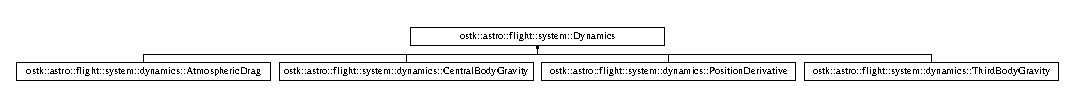
\includegraphics[height=0.957265cm]{classostk_1_1astro_1_1flight_1_1system_1_1_dynamics}
\end{center}
\end{figure}
\doxysubsection*{Classes}
\begin{DoxyCompactItemize}
\item 
struct \mbox{\hyperlink{structostk_1_1astro_1_1flight_1_1system_1_1_dynamics_1_1_context}{Context}}
\end{DoxyCompactItemize}
\doxysubsection*{Public Member Functions}
\begin{DoxyCompactItemize}
\item 
\mbox{\hyperlink{classostk_1_1astro_1_1flight_1_1system_1_1_dynamics_a3af17a36f06f2518e4a686148d40691c}{Dynamics}} (const String \&a\+Name=String\+::\+Empty())
\begin{DoxyCompactList}\small\item\em Constructor. \end{DoxyCompactList}\item 
virtual \mbox{\hyperlink{classostk_1_1astro_1_1flight_1_1system_1_1_dynamics_a16cee6671675f69baa685bfe2c918052}{$\sim$\+Dynamics}} ()
\begin{DoxyCompactList}\small\item\em Destructor. \end{DoxyCompactList}\item 
String \mbox{\hyperlink{classostk_1_1astro_1_1flight_1_1system_1_1_dynamics_a66734583c7858726da890f6e91273b8b}{get\+Name}} () const
\begin{DoxyCompactList}\small\item\em Get name. \end{DoxyCompactList}\item 
virtual void \mbox{\hyperlink{classostk_1_1astro_1_1flight_1_1system_1_1_dynamics_a01cf369daf419b0f9864f0e1d8d90e24}{print}} (std\+::ostream \&an\+Output\+Stream, bool display\+Decorator=true) const
\begin{DoxyCompactList}\small\item\em Print dynamics. \end{DoxyCompactList}\item 
virtual bool \mbox{\hyperlink{classostk_1_1astro_1_1flight_1_1system_1_1_dynamics_a13160e001990a6ce8db807e39b8f97df}{is\+Defined}} () const =0
\begin{DoxyCompactList}\small\item\em Check if dynamics is defined (pure virtual) \end{DoxyCompactList}\item 
virtual Array$<$ Shared$<$ const \mbox{\hyperlink{classostk_1_1astro_1_1trajectory_1_1state_1_1_coordinates_subset}{Coordinates\+Subset}} $>$ $>$ \mbox{\hyperlink{classostk_1_1astro_1_1flight_1_1system_1_1_dynamics_a4227a9bf26bde9932c0d818a67972076}{get\+Read\+Coordinates\+Subsets}} () const =0
\begin{DoxyCompactList}\small\item\em Return the coordinates subsets that the instance reads from. \end{DoxyCompactList}\item 
virtual Array$<$ Shared$<$ const \mbox{\hyperlink{classostk_1_1astro_1_1trajectory_1_1state_1_1_coordinates_subset}{Coordinates\+Subset}} $>$ $>$ \mbox{\hyperlink{classostk_1_1astro_1_1flight_1_1system_1_1_dynamics_a0f64bb21af5bc827763a8c3c422d0dbb}{get\+Write\+Coordinates\+Subsets}} () const =0
\begin{DoxyCompactList}\small\item\em Return the coordinates subsets that the instance writes to. \end{DoxyCompactList}\item 
virtual Vector\+Xd \mbox{\hyperlink{classostk_1_1astro_1_1flight_1_1system_1_1_dynamics_a945e44635ba9038b1a3a198deb1b1184}{compute\+Contribution}} (const Instant \&an\+Instant, const Vector\+Xd \&x, const Shared$<$ const Frame $>$ \&a\+Frame\+S\+Ptr) const =0
\begin{DoxyCompactList}\small\item\em Compute the contribution to the state derivative. \end{DoxyCompactList}\end{DoxyCompactItemize}
\doxysubsection*{Static Public Member Functions}
\begin{DoxyCompactItemize}
\item 
static Numerical\+Solver\+::\+System\+Of\+Equations\+Wrapper \mbox{\hyperlink{classostk_1_1astro_1_1flight_1_1system_1_1_dynamics_ad080ac5f6418af347f74db186052e2f6}{Get\+System\+Of\+Equations}} (const Array$<$ \mbox{\hyperlink{structostk_1_1astro_1_1flight_1_1system_1_1_dynamics_1_1_context}{Context}} $>$ \&a\+Context\+Array, const Instant \&an\+Instant, const Shared$<$ const Frame $>$ \&a\+Frame\+S\+Ptr)
\begin{DoxyCompactList}\small\item\em Get system of equations wrapper. \end{DoxyCompactList}\end{DoxyCompactItemize}
\doxysubsection*{Friends}
\begin{DoxyCompactItemize}
\item 
std\+::ostream \& \mbox{\hyperlink{classostk_1_1astro_1_1flight_1_1system_1_1_dynamics_aad1f02b40439704299193e464ba6e579}{operator$<$$<$}} (std\+::ostream \&an\+Output\+Stream, const \mbox{\hyperlink{classostk_1_1astro_1_1flight_1_1system_1_1_dynamics}{Dynamics}} \&a\+Dynamics)
\begin{DoxyCompactList}\small\item\em Output stream operator. \end{DoxyCompactList}\end{DoxyCompactItemize}


\doxysubsection{Detailed Description}
Define a dynamical system subject to equations of motion. 

\doxysubsection{Constructor \& Destructor Documentation}
\mbox{\Hypertarget{classostk_1_1astro_1_1flight_1_1system_1_1_dynamics_a3af17a36f06f2518e4a686148d40691c}\label{classostk_1_1astro_1_1flight_1_1system_1_1_dynamics_a3af17a36f06f2518e4a686148d40691c}} 
\index{ostk::astro::flight::system::Dynamics@{ostk::astro::flight::system::Dynamics}!Dynamics@{Dynamics}}
\index{Dynamics@{Dynamics}!ostk::astro::flight::system::Dynamics@{ostk::astro::flight::system::Dynamics}}
\doxysubsubsection{\texorpdfstring{Dynamics()}{Dynamics()}}
{\footnotesize\ttfamily ostk\+::astro\+::flight\+::system\+::\+Dynamics\+::\+Dynamics (\begin{DoxyParamCaption}\item[{const String \&}]{a\+Name = {\ttfamily String\+:\+:Empty()} }\end{DoxyParamCaption})}



Constructor. 


\begin{DoxyParams}[1]{Parameters}
\mbox{\texttt{ in}}  & {\em a\+Name} & A name \\
\hline
\end{DoxyParams}
\mbox{\Hypertarget{classostk_1_1astro_1_1flight_1_1system_1_1_dynamics_a16cee6671675f69baa685bfe2c918052}\label{classostk_1_1astro_1_1flight_1_1system_1_1_dynamics_a16cee6671675f69baa685bfe2c918052}} 
\index{ostk::astro::flight::system::Dynamics@{ostk::astro::flight::system::Dynamics}!````~Dynamics@{$\sim$Dynamics}}
\index{````~Dynamics@{$\sim$Dynamics}!ostk::astro::flight::system::Dynamics@{ostk::astro::flight::system::Dynamics}}
\doxysubsubsection{\texorpdfstring{$\sim$Dynamics()}{~Dynamics()}}
{\footnotesize\ttfamily ostk\+::astro\+::flight\+::system\+::\+Dynamics\+::$\sim$\+Dynamics (\begin{DoxyParamCaption}{ }\end{DoxyParamCaption})\hspace{0.3cm}{\ttfamily [virtual]}}



Destructor. 



\doxysubsection{Member Function Documentation}
\mbox{\Hypertarget{classostk_1_1astro_1_1flight_1_1system_1_1_dynamics_a945e44635ba9038b1a3a198deb1b1184}\label{classostk_1_1astro_1_1flight_1_1system_1_1_dynamics_a945e44635ba9038b1a3a198deb1b1184}} 
\index{ostk::astro::flight::system::Dynamics@{ostk::astro::flight::system::Dynamics}!computeContribution@{computeContribution}}
\index{computeContribution@{computeContribution}!ostk::astro::flight::system::Dynamics@{ostk::astro::flight::system::Dynamics}}
\doxysubsubsection{\texorpdfstring{computeContribution()}{computeContribution()}}
{\footnotesize\ttfamily virtual Vector\+Xd ostk\+::astro\+::flight\+::system\+::\+Dynamics\+::compute\+Contribution (\begin{DoxyParamCaption}\item[{const Instant \&}]{an\+Instant,  }\item[{const Vector\+Xd \&}]{x,  }\item[{const Shared$<$ const Frame $>$ \&}]{a\+Frame\+S\+Ptr }\end{DoxyParamCaption}) const\hspace{0.3cm}{\ttfamily [pure virtual]}}



Compute the contribution to the state derivative. 


\begin{DoxyParams}{Parameters}
{\em an\+Instant} & An instant \\
\hline
{\em x} & The reduced state vector (this vector will follow the structure determined by the \textquotesingle{}read\textquotesingle{} coordinate subsets) \\
\hline
{\em a\+Frame\+S\+Ptr} & The frame in which the state vector is expressed\\
\hline
\end{DoxyParams}
\begin{DoxyReturn}{Returns}
The reduced derivative state vector (this vector must follow the structure determined by the \textquotesingle{}write\textquotesingle{} coordinate subsets) expressed in the given frame 
\end{DoxyReturn}


Implemented in \mbox{\hyperlink{classostk_1_1astro_1_1flight_1_1system_1_1dynamics_1_1thruster_1_1_constant_thrust_a822a9a48aaab3647475f5c007ed61ca8}{ostk\+::astro\+::flight\+::system\+::dynamics\+::thruster\+::\+Constant\+Thrust}}, \mbox{\hyperlink{classostk_1_1astro_1_1flight_1_1system_1_1dynamics_1_1_atmospheric_drag_a427bf34a0302a40163a913c659f230bf}{ostk\+::astro\+::flight\+::system\+::dynamics\+::\+Atmospheric\+Drag}}, \mbox{\hyperlink{classostk_1_1astro_1_1flight_1_1system_1_1dynamics_1_1_central_body_gravity_a5975eec1a620758e4c3171ad6b683fad}{ostk\+::astro\+::flight\+::system\+::dynamics\+::\+Central\+Body\+Gravity}}, \mbox{\hyperlink{classostk_1_1astro_1_1flight_1_1system_1_1dynamics_1_1_third_body_gravity_a37f33dc52ed8be334e64ead1aceff384}{ostk\+::astro\+::flight\+::system\+::dynamics\+::\+Third\+Body\+Gravity}}, and \mbox{\hyperlink{classostk_1_1astro_1_1flight_1_1system_1_1dynamics_1_1_position_derivative_a7da63a2068fddf10429a2f0d935e15e6}{ostk\+::astro\+::flight\+::system\+::dynamics\+::\+Position\+Derivative}}.

\mbox{\Hypertarget{classostk_1_1astro_1_1flight_1_1system_1_1_dynamics_a66734583c7858726da890f6e91273b8b}\label{classostk_1_1astro_1_1flight_1_1system_1_1_dynamics_a66734583c7858726da890f6e91273b8b}} 
\index{ostk::astro::flight::system::Dynamics@{ostk::astro::flight::system::Dynamics}!getName@{getName}}
\index{getName@{getName}!ostk::astro::flight::system::Dynamics@{ostk::astro::flight::system::Dynamics}}
\doxysubsubsection{\texorpdfstring{getName()}{getName()}}
{\footnotesize\ttfamily String ostk\+::astro\+::flight\+::system\+::\+Dynamics\+::get\+Name (\begin{DoxyParamCaption}{ }\end{DoxyParamCaption}) const}



Get name. 

\begin{DoxyReturn}{Returns}
Name of \mbox{\hyperlink{classostk_1_1astro_1_1flight_1_1system_1_1_dynamics}{Dynamics}} 
\end{DoxyReturn}
\mbox{\Hypertarget{classostk_1_1astro_1_1flight_1_1system_1_1_dynamics_a4227a9bf26bde9932c0d818a67972076}\label{classostk_1_1astro_1_1flight_1_1system_1_1_dynamics_a4227a9bf26bde9932c0d818a67972076}} 
\index{ostk::astro::flight::system::Dynamics@{ostk::astro::flight::system::Dynamics}!getReadCoordinatesSubsets@{getReadCoordinatesSubsets}}
\index{getReadCoordinatesSubsets@{getReadCoordinatesSubsets}!ostk::astro::flight::system::Dynamics@{ostk::astro::flight::system::Dynamics}}
\doxysubsubsection{\texorpdfstring{getReadCoordinatesSubsets()}{getReadCoordinatesSubsets()}}
{\footnotesize\ttfamily virtual Array$<$Shared$<$const \mbox{\hyperlink{classostk_1_1astro_1_1trajectory_1_1state_1_1_coordinates_subset}{Coordinates\+Subset}}$>$ $>$ ostk\+::astro\+::flight\+::system\+::\+Dynamics\+::get\+Read\+Coordinates\+Subsets (\begin{DoxyParamCaption}{ }\end{DoxyParamCaption}) const\hspace{0.3cm}{\ttfamily [pure virtual]}}



Return the coordinates subsets that the instance reads from. 

\begin{DoxyReturn}{Returns}
The coordinates subsets that the instance reads from 
\end{DoxyReturn}


Implemented in \mbox{\hyperlink{classostk_1_1astro_1_1flight_1_1system_1_1dynamics_1_1thruster_1_1_constant_thrust_aabb7d62591b4babf94ed2ad080c4cff6}{ostk\+::astro\+::flight\+::system\+::dynamics\+::thruster\+::\+Constant\+Thrust}}, \mbox{\hyperlink{classostk_1_1astro_1_1flight_1_1system_1_1dynamics_1_1_atmospheric_drag_a6da1f0ae0221d5cdc9d421711530c73d}{ostk\+::astro\+::flight\+::system\+::dynamics\+::\+Atmospheric\+Drag}}, \mbox{\hyperlink{classostk_1_1astro_1_1flight_1_1system_1_1dynamics_1_1_central_body_gravity_ac3f486b78da8729947b5ed5faa18cc1f}{ostk\+::astro\+::flight\+::system\+::dynamics\+::\+Central\+Body\+Gravity}}, \mbox{\hyperlink{classostk_1_1astro_1_1flight_1_1system_1_1dynamics_1_1_third_body_gravity_acfbbe20757d4e0d4b0480915ca8f7789}{ostk\+::astro\+::flight\+::system\+::dynamics\+::\+Third\+Body\+Gravity}}, and \mbox{\hyperlink{classostk_1_1astro_1_1flight_1_1system_1_1dynamics_1_1_position_derivative_a840e0857864d8caa0c4dad8304bfbb59}{ostk\+::astro\+::flight\+::system\+::dynamics\+::\+Position\+Derivative}}.

\mbox{\Hypertarget{classostk_1_1astro_1_1flight_1_1system_1_1_dynamics_ad080ac5f6418af347f74db186052e2f6}\label{classostk_1_1astro_1_1flight_1_1system_1_1_dynamics_ad080ac5f6418af347f74db186052e2f6}} 
\index{ostk::astro::flight::system::Dynamics@{ostk::astro::flight::system::Dynamics}!GetSystemOfEquations@{GetSystemOfEquations}}
\index{GetSystemOfEquations@{GetSystemOfEquations}!ostk::astro::flight::system::Dynamics@{ostk::astro::flight::system::Dynamics}}
\doxysubsubsection{\texorpdfstring{GetSystemOfEquations()}{GetSystemOfEquations()}}
{\footnotesize\ttfamily Numerical\+Solver\+::\+System\+Of\+Equations\+Wrapper ostk\+::astro\+::flight\+::system\+::\+Dynamics\+::\+Get\+System\+Of\+Equations (\begin{DoxyParamCaption}\item[{const Array$<$ \mbox{\hyperlink{structostk_1_1astro_1_1flight_1_1system_1_1_dynamics_1_1_context}{Context}} $>$ \&}]{a\+Context\+Array,  }\item[{const Instant \&}]{an\+Instant,  }\item[{const Shared$<$ const Frame $>$ \&}]{a\+Frame\+S\+Ptr }\end{DoxyParamCaption})\hspace{0.3cm}{\ttfamily [static]}}



Get system of equations wrapper. 


\begin{DoxyParams}[1]{Parameters}
\mbox{\texttt{ in}}  & {\em a\+Context\+Array} & An array of \mbox{\hyperlink{classostk_1_1astro_1_1flight_1_1system_1_1_dynamics}{Dynamics}} Information \\
\hline
\mbox{\texttt{ in}}  & {\em an\+Instant} & An instant \\
\hline
\mbox{\texttt{ in}}  & {\em a\+Frame\+S\+Ptr} & The reference frame in which dynamic equations are resolved\\
\hline
\end{DoxyParams}
\begin{DoxyReturn}{Returns}
std\+::function$<$void(const std\+::vector$<$double$>$\&, std\+::vector$<$double$>$\&, const double)$>$ 
\end{DoxyReturn}
\mbox{\Hypertarget{classostk_1_1astro_1_1flight_1_1system_1_1_dynamics_a0f64bb21af5bc827763a8c3c422d0dbb}\label{classostk_1_1astro_1_1flight_1_1system_1_1_dynamics_a0f64bb21af5bc827763a8c3c422d0dbb}} 
\index{ostk::astro::flight::system::Dynamics@{ostk::astro::flight::system::Dynamics}!getWriteCoordinatesSubsets@{getWriteCoordinatesSubsets}}
\index{getWriteCoordinatesSubsets@{getWriteCoordinatesSubsets}!ostk::astro::flight::system::Dynamics@{ostk::astro::flight::system::Dynamics}}
\doxysubsubsection{\texorpdfstring{getWriteCoordinatesSubsets()}{getWriteCoordinatesSubsets()}}
{\footnotesize\ttfamily virtual Array$<$Shared$<$const \mbox{\hyperlink{classostk_1_1astro_1_1trajectory_1_1state_1_1_coordinates_subset}{Coordinates\+Subset}}$>$ $>$ ostk\+::astro\+::flight\+::system\+::\+Dynamics\+::get\+Write\+Coordinates\+Subsets (\begin{DoxyParamCaption}{ }\end{DoxyParamCaption}) const\hspace{0.3cm}{\ttfamily [pure virtual]}}



Return the coordinates subsets that the instance writes to. 

\begin{DoxyReturn}{Returns}
The coordinates subsets that the instance writes to 
\end{DoxyReturn}


Implemented in \mbox{\hyperlink{classostk_1_1astro_1_1flight_1_1system_1_1dynamics_1_1thruster_1_1_constant_thrust_af06c119a12a2576579aba69a75d7d7d9}{ostk\+::astro\+::flight\+::system\+::dynamics\+::thruster\+::\+Constant\+Thrust}}, \mbox{\hyperlink{classostk_1_1astro_1_1flight_1_1system_1_1dynamics_1_1_atmospheric_drag_a645abdc0fc1f2fce2824db69c57c785e}{ostk\+::astro\+::flight\+::system\+::dynamics\+::\+Atmospheric\+Drag}}, \mbox{\hyperlink{classostk_1_1astro_1_1flight_1_1system_1_1dynamics_1_1_central_body_gravity_a18e38c5a8704c4f5de48dfee9e7b15d4}{ostk\+::astro\+::flight\+::system\+::dynamics\+::\+Central\+Body\+Gravity}}, \mbox{\hyperlink{classostk_1_1astro_1_1flight_1_1system_1_1dynamics_1_1_third_body_gravity_ab88f4e3145fb9be25acede6aeb85ebf6}{ostk\+::astro\+::flight\+::system\+::dynamics\+::\+Third\+Body\+Gravity}}, and \mbox{\hyperlink{classostk_1_1astro_1_1flight_1_1system_1_1dynamics_1_1_position_derivative_a3860c4b65ae4e2841e13716595bdbfe9}{ostk\+::astro\+::flight\+::system\+::dynamics\+::\+Position\+Derivative}}.

\mbox{\Hypertarget{classostk_1_1astro_1_1flight_1_1system_1_1_dynamics_a13160e001990a6ce8db807e39b8f97df}\label{classostk_1_1astro_1_1flight_1_1system_1_1_dynamics_a13160e001990a6ce8db807e39b8f97df}} 
\index{ostk::astro::flight::system::Dynamics@{ostk::astro::flight::system::Dynamics}!isDefined@{isDefined}}
\index{isDefined@{isDefined}!ostk::astro::flight::system::Dynamics@{ostk::astro::flight::system::Dynamics}}
\doxysubsubsection{\texorpdfstring{isDefined()}{isDefined()}}
{\footnotesize\ttfamily virtual bool ostk\+::astro\+::flight\+::system\+::\+Dynamics\+::is\+Defined (\begin{DoxyParamCaption}{ }\end{DoxyParamCaption}) const\hspace{0.3cm}{\ttfamily [pure virtual]}}



Check if dynamics is defined (pure virtual) 

\begin{DoxyReturn}{Returns}
True if dynamics is defined 
\end{DoxyReturn}


Implemented in \mbox{\hyperlink{classostk_1_1astro_1_1flight_1_1system_1_1dynamics_1_1thruster_1_1_constant_thrust_ad4841b0ee3d279cd7fac05a2cdb7ec03}{ostk\+::astro\+::flight\+::system\+::dynamics\+::thruster\+::\+Constant\+Thrust}}, \mbox{\hyperlink{classostk_1_1astro_1_1flight_1_1system_1_1dynamics_1_1_atmospheric_drag_a279876706fe6b8438f7c3507bef01592}{ostk\+::astro\+::flight\+::system\+::dynamics\+::\+Atmospheric\+Drag}}, \mbox{\hyperlink{classostk_1_1astro_1_1flight_1_1system_1_1dynamics_1_1_central_body_gravity_ac3c0f63c901827bdcff58359c2081c66}{ostk\+::astro\+::flight\+::system\+::dynamics\+::\+Central\+Body\+Gravity}}, \mbox{\hyperlink{classostk_1_1astro_1_1flight_1_1system_1_1dynamics_1_1_third_body_gravity_ad5b8acb98124efefd4a94ae2ed222e7e}{ostk\+::astro\+::flight\+::system\+::dynamics\+::\+Third\+Body\+Gravity}}, \mbox{\hyperlink{classostk_1_1astro_1_1flight_1_1system_1_1dynamics_1_1_position_derivative_ac9b701dffe0b64ce0931e4125e379fa7}{ostk\+::astro\+::flight\+::system\+::dynamics\+::\+Position\+Derivative}}, and \mbox{\hyperlink{classostk_1_1astro_1_1flight_1_1system_1_1dynamics_1_1_thruster_aa4c53c7aae3f9073954b7e3475f70e13}{ostk\+::astro\+::flight\+::system\+::dynamics\+::\+Thruster}}.

\mbox{\Hypertarget{classostk_1_1astro_1_1flight_1_1system_1_1_dynamics_a01cf369daf419b0f9864f0e1d8d90e24}\label{classostk_1_1astro_1_1flight_1_1system_1_1_dynamics_a01cf369daf419b0f9864f0e1d8d90e24}} 
\index{ostk::astro::flight::system::Dynamics@{ostk::astro::flight::system::Dynamics}!print@{print}}
\index{print@{print}!ostk::astro::flight::system::Dynamics@{ostk::astro::flight::system::Dynamics}}
\doxysubsubsection{\texorpdfstring{print()}{print()}}
{\footnotesize\ttfamily void ostk\+::astro\+::flight\+::system\+::\+Dynamics\+::print (\begin{DoxyParamCaption}\item[{std\+::ostream \&}]{an\+Output\+Stream,  }\item[{bool}]{display\+Decorator = {\ttfamily true} }\end{DoxyParamCaption}) const\hspace{0.3cm}{\ttfamily [virtual]}}



Print dynamics. 


\begin{DoxyParams}[1]{Parameters}
\mbox{\texttt{ in}}  & {\em an\+Output\+Stream} & An output stream \\
\hline
\mbox{\texttt{ in}}  & {\em (optional)} & display\+Decorators If true, display decorators \\
\hline
\end{DoxyParams}


Reimplemented in \mbox{\hyperlink{classostk_1_1astro_1_1flight_1_1system_1_1dynamics_1_1thruster_1_1_constant_thrust_a893856d92c1b34e9007b7549209d7ec8}{ostk\+::astro\+::flight\+::system\+::dynamics\+::thruster\+::\+Constant\+Thrust}}, \mbox{\hyperlink{classostk_1_1astro_1_1flight_1_1system_1_1dynamics_1_1_atmospheric_drag_adfca0c807bb765365ac69a456efde5bf}{ostk\+::astro\+::flight\+::system\+::dynamics\+::\+Atmospheric\+Drag}}, \mbox{\hyperlink{classostk_1_1astro_1_1flight_1_1system_1_1dynamics_1_1_central_body_gravity_a2fc0c0e4676244da1ff05a31ca632a7c}{ostk\+::astro\+::flight\+::system\+::dynamics\+::\+Central\+Body\+Gravity}}, \mbox{\hyperlink{classostk_1_1astro_1_1flight_1_1system_1_1dynamics_1_1_third_body_gravity_acc3898d92a779f5a3a111f0e0d4a27ae}{ostk\+::astro\+::flight\+::system\+::dynamics\+::\+Third\+Body\+Gravity}}, \mbox{\hyperlink{classostk_1_1astro_1_1flight_1_1system_1_1dynamics_1_1_position_derivative_a7d9b302e022c8b31063a4a7e9fb2ef31}{ostk\+::astro\+::flight\+::system\+::dynamics\+::\+Position\+Derivative}}, and \mbox{\hyperlink{classostk_1_1astro_1_1flight_1_1system_1_1dynamics_1_1_thruster_a13808c5958b79bbe766e312ffc1e947e}{ostk\+::astro\+::flight\+::system\+::dynamics\+::\+Thruster}}.



\doxysubsection{Friends And Related Function Documentation}
\mbox{\Hypertarget{classostk_1_1astro_1_1flight_1_1system_1_1_dynamics_aad1f02b40439704299193e464ba6e579}\label{classostk_1_1astro_1_1flight_1_1system_1_1_dynamics_aad1f02b40439704299193e464ba6e579}} 
\index{ostk::astro::flight::system::Dynamics@{ostk::astro::flight::system::Dynamics}!operator$<$$<$@{operator$<$$<$}}
\index{operator$<$$<$@{operator$<$$<$}!ostk::astro::flight::system::Dynamics@{ostk::astro::flight::system::Dynamics}}
\doxysubsubsection{\texorpdfstring{operator$<$$<$}{operator<<}}
{\footnotesize\ttfamily std\+::ostream\& operator$<$$<$ (\begin{DoxyParamCaption}\item[{std\+::ostream \&}]{an\+Output\+Stream,  }\item[{const \mbox{\hyperlink{classostk_1_1astro_1_1flight_1_1system_1_1_dynamics}{Dynamics}} \&}]{a\+Dynamics }\end{DoxyParamCaption})\hspace{0.3cm}{\ttfamily [friend]}}



Output stream operator. 


\begin{DoxyCode}{0}
\DoxyCodeLine{std::cout << \mbox{\hyperlink{classostk_1_1astro_1_1flight_1_1system_1_1_dynamics_a3af17a36f06f2518e4a686148d40691c}{Dynamics}}(...) ;}
\end{DoxyCode}



\begin{DoxyParams}[1]{Parameters}
\mbox{\texttt{ in}}  & {\em an\+Output\+Stream} & An output stream \\
\hline
\mbox{\texttt{ in}}  & {\em a\+Dynamics} & A \mbox{\hyperlink{classostk_1_1astro_1_1flight_1_1system_1_1_dynamics}{Dynamics}} \\
\hline
\end{DoxyParams}
\begin{DoxyReturn}{Returns}
A reference to output stream 
\end{DoxyReturn}


The documentation for this class was generated from the following files\+:\begin{DoxyCompactItemize}
\item 
include/\+Open\+Space\+Toolkit/\+Astrodynamics/\+Flight/\+System/\mbox{\hyperlink{_dynamics_8hpp}{Dynamics.\+hpp}}\item 
src/\+Open\+Space\+Toolkit/\+Astrodynamics/\+Flight/\+System/\mbox{\hyperlink{_dynamics_8cpp}{Dynamics.\+cpp}}\end{DoxyCompactItemize}

\hypertarget{classostk_1_1astro_1_1access_1_1_generator}{}\doxysection{ostk\+::astro\+::access\+::Generator Class Reference}
\label{classostk_1_1astro_1_1access_1_1_generator}\index{ostk::astro::access::Generator@{ostk::astro::access::Generator}}


{\ttfamily \#include $<$Generator.\+hpp$>$}

\doxysubsection*{Public Member Functions}
\begin{DoxyCompactItemize}
\item 
\mbox{\hyperlink{classostk_1_1astro_1_1access_1_1_generator_a009da655bc3cc6232cd9986275cc5731}{Generator}} (const Environment \&an\+Environment, const Duration \&a\+Step=\mbox{\hyperlink{_generator_8hpp_a7ce1d4cc8c33e65c078f721b17b975ea}{D\+E\+F\+A\+U\+L\+T\+\_\+\+S\+T\+EP}}, const Duration \&a\+Tolerance=\mbox{\hyperlink{_generator_8hpp_a0e355e0dcb761f1b89524e0e77fd14bd}{D\+E\+F\+A\+U\+L\+T\+\_\+\+T\+O\+L\+E\+R\+A\+N\+CE}})
\item 
\mbox{\hyperlink{classostk_1_1astro_1_1access_1_1_generator_a4997c5e017539c2e5a735ed9a152ae8a}{Generator}} (const Environment \&an\+Environment, const std\+::function$<$ bool(const A\+ER \&)$>$ \&an\+Aer\+Filter, const std\+::function$<$ bool(const \mbox{\hyperlink{classostk_1_1astro_1_1_access}{Access}} \&)$>$ \&an\+Access\+Filter=\{\}, const std\+::function$<$ bool(const \mbox{\hyperlink{classostk_1_1astro_1_1trajectory_1_1_state}{State}} \&, const \mbox{\hyperlink{classostk_1_1astro_1_1trajectory_1_1_state}{State}} \&)$>$ \&a\+State\+Filter=\{\}, const Duration \&a\+Step=\mbox{\hyperlink{_generator_8hpp_a7ce1d4cc8c33e65c078f721b17b975ea}{D\+E\+F\+A\+U\+L\+T\+\_\+\+S\+T\+EP}}, const Duration \&a\+Tolerance=\mbox{\hyperlink{_generator_8hpp_a0e355e0dcb761f1b89524e0e77fd14bd}{D\+E\+F\+A\+U\+L\+T\+\_\+\+T\+O\+L\+E\+R\+A\+N\+CE}})
\item 
bool \mbox{\hyperlink{classostk_1_1astro_1_1access_1_1_generator_a36d805bcebc2997daa0a1d89f5240277}{is\+Defined}} () const
\item 
Duration \mbox{\hyperlink{classostk_1_1astro_1_1access_1_1_generator_a1fa5d363b74c6badf4f925174affd91c}{get\+Step}} () const
\item 
Duration \mbox{\hyperlink{classostk_1_1astro_1_1access_1_1_generator_a47010380af2aa5b0ffa9864edb12ff5d}{get\+Tolerance}} () const
\item 
Array$<$ \mbox{\hyperlink{classostk_1_1astro_1_1_access}{Access}} $>$ \mbox{\hyperlink{classostk_1_1astro_1_1access_1_1_generator_a3624c39c3ffa4588c40a687ccc4b8145}{compute\+Accesses}} (const physics\+::time\+::\+Interval \&an\+Interval, const \mbox{\hyperlink{classostk_1_1astro_1_1_trajectory}{Trajectory}} \&a\+From\+Trajectory, const \mbox{\hyperlink{classostk_1_1astro_1_1_trajectory}{Trajectory}} \&a\+To\+Trajectory) const
\item 
void \mbox{\hyperlink{classostk_1_1astro_1_1access_1_1_generator_a4c0cb8f1e59364029e88078c423cd96b}{set\+Step}} (const Duration \&a\+Step)
\item 
void \mbox{\hyperlink{classostk_1_1astro_1_1access_1_1_generator_a9590a1ebb05d28f7934f8ccafbd02a60}{set\+Tolerance}} (const Duration \&a\+Tolerance)
\item 
void \mbox{\hyperlink{classostk_1_1astro_1_1access_1_1_generator_a4d82f15eb2da1fbf7c74b3136eed3301}{set\+Aer\+Filter}} (const std\+::function$<$ bool(const A\+ER \&)$>$ \&an\+Aer\+Filter)
\item 
void \mbox{\hyperlink{classostk_1_1astro_1_1access_1_1_generator_ade3c6b8b5afe0f850e3531d715eac826}{set\+Access\+Filter}} (const std\+::function$<$ bool(const \mbox{\hyperlink{classostk_1_1astro_1_1_access}{Access}} \&)$>$ \&an\+Access\+Filter)
\item 
void \mbox{\hyperlink{classostk_1_1astro_1_1access_1_1_generator_a2e67d180ec17450e460be15f24a1d84d}{set\+State\+Filter}} (const std\+::function$<$ bool(const \mbox{\hyperlink{classostk_1_1astro_1_1trajectory_1_1_state}{State}} \&, const \mbox{\hyperlink{classostk_1_1astro_1_1trajectory_1_1_state}{State}} \&)$>$ \&a\+State\+Filter)
\end{DoxyCompactItemize}
\doxysubsection*{Static Public Member Functions}
\begin{DoxyCompactItemize}
\item 
static \mbox{\hyperlink{classostk_1_1astro_1_1access_1_1_generator}{Generator}} \mbox{\hyperlink{classostk_1_1astro_1_1access_1_1_generator_a1fb2dd3d88187da24482168337a23ade}{Undefined}} ()
\item 
static \mbox{\hyperlink{classostk_1_1astro_1_1access_1_1_generator}{Generator}} \mbox{\hyperlink{classostk_1_1astro_1_1access_1_1_generator_aececdcffcfea35feb07d9214752e6995}{Aer\+Ranges}} (const Interval$<$ Real $>$ \&an\+Azimuth\+Range, const Interval$<$ Real $>$ \&an\+Elevation\+Range, const Interval$<$ Real $>$ \&a\+Range\+Range, const Environment \&an\+Environment)
\begin{DoxyCompactList}\small\item\em Constructs an access generator with defined A\+ER ranges. \end{DoxyCompactList}\item 
static \mbox{\hyperlink{classostk_1_1astro_1_1access_1_1_generator}{Generator}} \mbox{\hyperlink{classostk_1_1astro_1_1access_1_1_generator_a023edbe897ad6db339dce2107821442f}{Aer\+Mask}} (const Map$<$ Real, Real $>$ \&an\+Azimuth\+Elevation\+Mask, const Interval$<$ Real $>$ \&a\+Range\+Range, const Environment \&an\+Environment)
\begin{DoxyCompactList}\small\item\em Constructs an access generator with a defined A\+ER mask. \end{DoxyCompactList}\end{DoxyCompactItemize}


\doxysubsection{Constructor \& Destructor Documentation}
\mbox{\Hypertarget{classostk_1_1astro_1_1access_1_1_generator_a009da655bc3cc6232cd9986275cc5731}\label{classostk_1_1astro_1_1access_1_1_generator_a009da655bc3cc6232cd9986275cc5731}} 
\index{ostk::astro::access::Generator@{ostk::astro::access::Generator}!Generator@{Generator}}
\index{Generator@{Generator}!ostk::astro::access::Generator@{ostk::astro::access::Generator}}
\doxysubsubsection{\texorpdfstring{Generator()}{Generator()}\hspace{0.1cm}{\footnotesize\ttfamily [1/2]}}
{\footnotesize\ttfamily ostk\+::astro\+::access\+::\+Generator\+::\+Generator (\begin{DoxyParamCaption}\item[{const Environment \&}]{an\+Environment,  }\item[{const Duration \&}]{a\+Step = {\ttfamily \mbox{\hyperlink{_generator_8hpp_a7ce1d4cc8c33e65c078f721b17b975ea}{D\+E\+F\+A\+U\+L\+T\+\_\+\+S\+T\+EP}}},  }\item[{const Duration \&}]{a\+Tolerance = {\ttfamily \mbox{\hyperlink{_generator_8hpp_a0e355e0dcb761f1b89524e0e77fd14bd}{D\+E\+F\+A\+U\+L\+T\+\_\+\+T\+O\+L\+E\+R\+A\+N\+CE}}} }\end{DoxyParamCaption})}

\mbox{\Hypertarget{classostk_1_1astro_1_1access_1_1_generator_a4997c5e017539c2e5a735ed9a152ae8a}\label{classostk_1_1astro_1_1access_1_1_generator_a4997c5e017539c2e5a735ed9a152ae8a}} 
\index{ostk::astro::access::Generator@{ostk::astro::access::Generator}!Generator@{Generator}}
\index{Generator@{Generator}!ostk::astro::access::Generator@{ostk::astro::access::Generator}}
\doxysubsubsection{\texorpdfstring{Generator()}{Generator()}\hspace{0.1cm}{\footnotesize\ttfamily [2/2]}}
{\footnotesize\ttfamily ostk\+::astro\+::access\+::\+Generator\+::\+Generator (\begin{DoxyParamCaption}\item[{const Environment \&}]{an\+Environment,  }\item[{const std\+::function$<$ bool(const A\+ER \&)$>$ \&}]{an\+Aer\+Filter,  }\item[{const std\+::function$<$ bool(const \mbox{\hyperlink{classostk_1_1astro_1_1_access}{Access}} \&)$>$ \&}]{an\+Access\+Filter = {\ttfamily \{\}},  }\item[{const std\+::function$<$ bool(const \mbox{\hyperlink{classostk_1_1astro_1_1trajectory_1_1_state}{State}} \&, const \mbox{\hyperlink{classostk_1_1astro_1_1trajectory_1_1_state}{State}} \&)$>$ \&}]{a\+State\+Filter = {\ttfamily \{\}},  }\item[{const Duration \&}]{a\+Step = {\ttfamily \mbox{\hyperlink{_generator_8hpp_a7ce1d4cc8c33e65c078f721b17b975ea}{D\+E\+F\+A\+U\+L\+T\+\_\+\+S\+T\+EP}}},  }\item[{const Duration \&}]{a\+Tolerance = {\ttfamily \mbox{\hyperlink{_generator_8hpp_a0e355e0dcb761f1b89524e0e77fd14bd}{D\+E\+F\+A\+U\+L\+T\+\_\+\+T\+O\+L\+E\+R\+A\+N\+CE}}} }\end{DoxyParamCaption})}



\doxysubsection{Member Function Documentation}
\mbox{\Hypertarget{classostk_1_1astro_1_1access_1_1_generator_a023edbe897ad6db339dce2107821442f}\label{classostk_1_1astro_1_1access_1_1_generator_a023edbe897ad6db339dce2107821442f}} 
\index{ostk::astro::access::Generator@{ostk::astro::access::Generator}!AerMask@{AerMask}}
\index{AerMask@{AerMask}!ostk::astro::access::Generator@{ostk::astro::access::Generator}}
\doxysubsubsection{\texorpdfstring{AerMask()}{AerMask()}}
{\footnotesize\ttfamily \mbox{\hyperlink{classostk_1_1astro_1_1access_1_1_generator}{Generator}} ostk\+::astro\+::access\+::\+Generator\+::\+Aer\+Mask (\begin{DoxyParamCaption}\item[{const Map$<$ Real, Real $>$ \&}]{an\+Azimuth\+Elevation\+Mask,  }\item[{const Interval$<$ Real $>$ \&}]{a\+Range\+Range,  }\item[{const Environment \&}]{an\+Environment }\end{DoxyParamCaption})\hspace{0.3cm}{\ttfamily [static]}}



Constructs an access generator with a defined A\+ER mask. 


\begin{DoxyParams}[1]{Parameters}
\mbox{\texttt{ in}}  & {\em an\+Azimuth\+Elevation\+Mask} & An azimuth-\/elevation mask \mbox{[}deg\mbox{]} \\
\hline
\mbox{\texttt{ in}}  & {\em a\+Range\+Range} & A range interval \mbox{[}m\mbox{]} \\
\hline
\mbox{\texttt{ in}}  & {\em an\+Environment} & An environment \\
\hline
\end{DoxyParams}
\begin{DoxyReturn}{Returns}
An access generator 
\end{DoxyReturn}
\mbox{\Hypertarget{classostk_1_1astro_1_1access_1_1_generator_aececdcffcfea35feb07d9214752e6995}\label{classostk_1_1astro_1_1access_1_1_generator_aececdcffcfea35feb07d9214752e6995}} 
\index{ostk::astro::access::Generator@{ostk::astro::access::Generator}!AerRanges@{AerRanges}}
\index{AerRanges@{AerRanges}!ostk::astro::access::Generator@{ostk::astro::access::Generator}}
\doxysubsubsection{\texorpdfstring{AerRanges()}{AerRanges()}}
{\footnotesize\ttfamily \mbox{\hyperlink{classostk_1_1astro_1_1access_1_1_generator}{Generator}} ostk\+::astro\+::access\+::\+Generator\+::\+Aer\+Ranges (\begin{DoxyParamCaption}\item[{const Interval$<$ Real $>$ \&}]{an\+Azimuth\+Range,  }\item[{const Interval$<$ Real $>$ \&}]{an\+Elevation\+Range,  }\item[{const Interval$<$ Real $>$ \&}]{a\+Range\+Range,  }\item[{const Environment \&}]{an\+Environment }\end{DoxyParamCaption})\hspace{0.3cm}{\ttfamily [static]}}



Constructs an access generator with defined A\+ER ranges. 


\begin{DoxyParams}[1]{Parameters}
\mbox{\texttt{ in}}  & {\em an\+Azimuth\+Range} & An azimuth interval \mbox{[}deg\mbox{]} \\
\hline
\mbox{\texttt{ in}}  & {\em an\+Elevation\+Range} & An elevation interval \mbox{[}deg\mbox{]} \\
\hline
\mbox{\texttt{ in}}  & {\em a\+Range\+Range} & A range interval \mbox{[}m\mbox{]} \\
\hline
\mbox{\texttt{ in}}  & {\em an\+Environment} & An environment \\
\hline
\end{DoxyParams}
\begin{DoxyReturn}{Returns}
An access generator 
\end{DoxyReturn}
\mbox{\Hypertarget{classostk_1_1astro_1_1access_1_1_generator_a3624c39c3ffa4588c40a687ccc4b8145}\label{classostk_1_1astro_1_1access_1_1_generator_a3624c39c3ffa4588c40a687ccc4b8145}} 
\index{ostk::astro::access::Generator@{ostk::astro::access::Generator}!computeAccesses@{computeAccesses}}
\index{computeAccesses@{computeAccesses}!ostk::astro::access::Generator@{ostk::astro::access::Generator}}
\doxysubsubsection{\texorpdfstring{computeAccesses()}{computeAccesses()}}
{\footnotesize\ttfamily Array$<$ \mbox{\hyperlink{classostk_1_1astro_1_1_access}{Access}} $>$ ostk\+::astro\+::access\+::\+Generator\+::compute\+Accesses (\begin{DoxyParamCaption}\item[{const physics\+::time\+::\+Interval \&}]{an\+Interval,  }\item[{const \mbox{\hyperlink{classostk_1_1astro_1_1_trajectory}{Trajectory}} \&}]{a\+From\+Trajectory,  }\item[{const \mbox{\hyperlink{classostk_1_1astro_1_1_trajectory}{Trajectory}} \&}]{a\+To\+Trajectory }\end{DoxyParamCaption}) const}

\mbox{\Hypertarget{classostk_1_1astro_1_1access_1_1_generator_a1fa5d363b74c6badf4f925174affd91c}\label{classostk_1_1astro_1_1access_1_1_generator_a1fa5d363b74c6badf4f925174affd91c}} 
\index{ostk::astro::access::Generator@{ostk::astro::access::Generator}!getStep@{getStep}}
\index{getStep@{getStep}!ostk::astro::access::Generator@{ostk::astro::access::Generator}}
\doxysubsubsection{\texorpdfstring{getStep()}{getStep()}}
{\footnotesize\ttfamily Duration ostk\+::astro\+::access\+::\+Generator\+::get\+Step (\begin{DoxyParamCaption}{ }\end{DoxyParamCaption}) const}

\mbox{\Hypertarget{classostk_1_1astro_1_1access_1_1_generator_a47010380af2aa5b0ffa9864edb12ff5d}\label{classostk_1_1astro_1_1access_1_1_generator_a47010380af2aa5b0ffa9864edb12ff5d}} 
\index{ostk::astro::access::Generator@{ostk::astro::access::Generator}!getTolerance@{getTolerance}}
\index{getTolerance@{getTolerance}!ostk::astro::access::Generator@{ostk::astro::access::Generator}}
\doxysubsubsection{\texorpdfstring{getTolerance()}{getTolerance()}}
{\footnotesize\ttfamily Duration ostk\+::astro\+::access\+::\+Generator\+::get\+Tolerance (\begin{DoxyParamCaption}{ }\end{DoxyParamCaption}) const}

\mbox{\Hypertarget{classostk_1_1astro_1_1access_1_1_generator_a36d805bcebc2997daa0a1d89f5240277}\label{classostk_1_1astro_1_1access_1_1_generator_a36d805bcebc2997daa0a1d89f5240277}} 
\index{ostk::astro::access::Generator@{ostk::astro::access::Generator}!isDefined@{isDefined}}
\index{isDefined@{isDefined}!ostk::astro::access::Generator@{ostk::astro::access::Generator}}
\doxysubsubsection{\texorpdfstring{isDefined()}{isDefined()}}
{\footnotesize\ttfamily bool ostk\+::astro\+::access\+::\+Generator\+::is\+Defined (\begin{DoxyParamCaption}{ }\end{DoxyParamCaption}) const}

\mbox{\Hypertarget{classostk_1_1astro_1_1access_1_1_generator_ade3c6b8b5afe0f850e3531d715eac826}\label{classostk_1_1astro_1_1access_1_1_generator_ade3c6b8b5afe0f850e3531d715eac826}} 
\index{ostk::astro::access::Generator@{ostk::astro::access::Generator}!setAccessFilter@{setAccessFilter}}
\index{setAccessFilter@{setAccessFilter}!ostk::astro::access::Generator@{ostk::astro::access::Generator}}
\doxysubsubsection{\texorpdfstring{setAccessFilter()}{setAccessFilter()}}
{\footnotesize\ttfamily void ostk\+::astro\+::access\+::\+Generator\+::set\+Access\+Filter (\begin{DoxyParamCaption}\item[{const std\+::function$<$ bool(const \mbox{\hyperlink{classostk_1_1astro_1_1_access}{Access}} \&)$>$ \&}]{an\+Access\+Filter }\end{DoxyParamCaption})}

\mbox{\Hypertarget{classostk_1_1astro_1_1access_1_1_generator_a4d82f15eb2da1fbf7c74b3136eed3301}\label{classostk_1_1astro_1_1access_1_1_generator_a4d82f15eb2da1fbf7c74b3136eed3301}} 
\index{ostk::astro::access::Generator@{ostk::astro::access::Generator}!setAerFilter@{setAerFilter}}
\index{setAerFilter@{setAerFilter}!ostk::astro::access::Generator@{ostk::astro::access::Generator}}
\doxysubsubsection{\texorpdfstring{setAerFilter()}{setAerFilter()}}
{\footnotesize\ttfamily void ostk\+::astro\+::access\+::\+Generator\+::set\+Aer\+Filter (\begin{DoxyParamCaption}\item[{const std\+::function$<$ bool(const A\+ER \&)$>$ \&}]{an\+Aer\+Filter }\end{DoxyParamCaption})}

\mbox{\Hypertarget{classostk_1_1astro_1_1access_1_1_generator_a2e67d180ec17450e460be15f24a1d84d}\label{classostk_1_1astro_1_1access_1_1_generator_a2e67d180ec17450e460be15f24a1d84d}} 
\index{ostk::astro::access::Generator@{ostk::astro::access::Generator}!setStateFilter@{setStateFilter}}
\index{setStateFilter@{setStateFilter}!ostk::astro::access::Generator@{ostk::astro::access::Generator}}
\doxysubsubsection{\texorpdfstring{setStateFilter()}{setStateFilter()}}
{\footnotesize\ttfamily void ostk\+::astro\+::access\+::\+Generator\+::set\+State\+Filter (\begin{DoxyParamCaption}\item[{const std\+::function$<$ bool(const \mbox{\hyperlink{classostk_1_1astro_1_1trajectory_1_1_state}{State}} \&, const \mbox{\hyperlink{classostk_1_1astro_1_1trajectory_1_1_state}{State}} \&)$>$ \&}]{a\+State\+Filter }\end{DoxyParamCaption})}

\mbox{\Hypertarget{classostk_1_1astro_1_1access_1_1_generator_a4c0cb8f1e59364029e88078c423cd96b}\label{classostk_1_1astro_1_1access_1_1_generator_a4c0cb8f1e59364029e88078c423cd96b}} 
\index{ostk::astro::access::Generator@{ostk::astro::access::Generator}!setStep@{setStep}}
\index{setStep@{setStep}!ostk::astro::access::Generator@{ostk::astro::access::Generator}}
\doxysubsubsection{\texorpdfstring{setStep()}{setStep()}}
{\footnotesize\ttfamily void ostk\+::astro\+::access\+::\+Generator\+::set\+Step (\begin{DoxyParamCaption}\item[{const Duration \&}]{a\+Step }\end{DoxyParamCaption})}

\mbox{\Hypertarget{classostk_1_1astro_1_1access_1_1_generator_a9590a1ebb05d28f7934f8ccafbd02a60}\label{classostk_1_1astro_1_1access_1_1_generator_a9590a1ebb05d28f7934f8ccafbd02a60}} 
\index{ostk::astro::access::Generator@{ostk::astro::access::Generator}!setTolerance@{setTolerance}}
\index{setTolerance@{setTolerance}!ostk::astro::access::Generator@{ostk::astro::access::Generator}}
\doxysubsubsection{\texorpdfstring{setTolerance()}{setTolerance()}}
{\footnotesize\ttfamily void ostk\+::astro\+::access\+::\+Generator\+::set\+Tolerance (\begin{DoxyParamCaption}\item[{const Duration \&}]{a\+Tolerance }\end{DoxyParamCaption})}

\mbox{\Hypertarget{classostk_1_1astro_1_1access_1_1_generator_a1fb2dd3d88187da24482168337a23ade}\label{classostk_1_1astro_1_1access_1_1_generator_a1fb2dd3d88187da24482168337a23ade}} 
\index{ostk::astro::access::Generator@{ostk::astro::access::Generator}!Undefined@{Undefined}}
\index{Undefined@{Undefined}!ostk::astro::access::Generator@{ostk::astro::access::Generator}}
\doxysubsubsection{\texorpdfstring{Undefined()}{Undefined()}}
{\footnotesize\ttfamily \mbox{\hyperlink{classostk_1_1astro_1_1access_1_1_generator}{Generator}} ostk\+::astro\+::access\+::\+Generator\+::\+Undefined (\begin{DoxyParamCaption}{ }\end{DoxyParamCaption})\hspace{0.3cm}{\ttfamily [static]}}



The documentation for this class was generated from the following files\+:\begin{DoxyCompactItemize}
\item 
include/\+Open\+Space\+Toolkit/\+Astrodynamics/\+Access/\mbox{\hyperlink{_generator_8hpp}{Generator.\+hpp}}\item 
src/\+Open\+Space\+Toolkit/\+Astrodynamics/\+Access/\mbox{\hyperlink{_generator_8cpp}{Generator.\+cpp}}\end{DoxyCompactItemize}

\hypertarget{structostk_1_1astro_1_1conjunction_1_1messages_1_1ccsds_1_1_c_d_m_1_1_header}{}\doxysection{ostk\+::astro\+::conjunction\+::messages\+::ccsds\+::C\+DM\+::Header Struct Reference}
\label{structostk_1_1astro_1_1conjunction_1_1messages_1_1ccsds_1_1_c_d_m_1_1_header}\index{ostk::astro::conjunction::messages::ccsds::CDM::Header@{ostk::astro::conjunction::messages::ccsds::CDM::Header}}


{\ttfamily \#include $<$C\+D\+M.\+hpp$>$}

\doxysubsection*{Public Attributes}
\begin{DoxyCompactItemize}
\item 
String \mbox{\hyperlink{structostk_1_1astro_1_1conjunction_1_1messages_1_1ccsds_1_1_c_d_m_1_1_header_a3050d7ef808f9ee8f10fd3346ffcb23f}{ccsds\+Cdm\+Version}}
\item 
String \mbox{\hyperlink{structostk_1_1astro_1_1conjunction_1_1messages_1_1ccsds_1_1_c_d_m_1_1_header_a5f903615e1e7bb48a7335ef4337a6218}{comment}} = String\+::\+Empty()
\item 
Instant \mbox{\hyperlink{structostk_1_1astro_1_1conjunction_1_1messages_1_1ccsds_1_1_c_d_m_1_1_header_a2188a4fc3aca51a6d96f3eedc5205d72}{creation\+Date}}
\item 
String \mbox{\hyperlink{structostk_1_1astro_1_1conjunction_1_1messages_1_1ccsds_1_1_c_d_m_1_1_header_aaff1cbfa0ac968d01e6f5d03a70a30ce}{originator}}
\item 
String \mbox{\hyperlink{structostk_1_1astro_1_1conjunction_1_1messages_1_1ccsds_1_1_c_d_m_1_1_header_aa82722c53756f396de0dafeeda1fc327}{message\+For}} = String\+::\+Empty()
\item 
String \mbox{\hyperlink{structostk_1_1astro_1_1conjunction_1_1messages_1_1ccsds_1_1_c_d_m_1_1_header_a9f8a18247622e0fa0b4394bfa51b501c}{message\+Id}}
\end{DoxyCompactItemize}


\doxysubsection{Member Data Documentation}
\mbox{\Hypertarget{structostk_1_1astro_1_1conjunction_1_1messages_1_1ccsds_1_1_c_d_m_1_1_header_a3050d7ef808f9ee8f10fd3346ffcb23f}\label{structostk_1_1astro_1_1conjunction_1_1messages_1_1ccsds_1_1_c_d_m_1_1_header_a3050d7ef808f9ee8f10fd3346ffcb23f}} 
\index{ostk::astro::conjunction::messages::ccsds::CDM::Header@{ostk::astro::conjunction::messages::ccsds::CDM::Header}!ccsdsCdmVersion@{ccsdsCdmVersion}}
\index{ccsdsCdmVersion@{ccsdsCdmVersion}!ostk::astro::conjunction::messages::ccsds::CDM::Header@{ostk::astro::conjunction::messages::ccsds::CDM::Header}}
\doxysubsubsection{\texorpdfstring{ccsdsCdmVersion}{ccsdsCdmVersion}}
{\footnotesize\ttfamily String ostk\+::astro\+::conjunction\+::messages\+::ccsds\+::\+C\+D\+M\+::\+Header\+::ccsds\+Cdm\+Version}

\mbox{\Hypertarget{structostk_1_1astro_1_1conjunction_1_1messages_1_1ccsds_1_1_c_d_m_1_1_header_a5f903615e1e7bb48a7335ef4337a6218}\label{structostk_1_1astro_1_1conjunction_1_1messages_1_1ccsds_1_1_c_d_m_1_1_header_a5f903615e1e7bb48a7335ef4337a6218}} 
\index{ostk::astro::conjunction::messages::ccsds::CDM::Header@{ostk::astro::conjunction::messages::ccsds::CDM::Header}!comment@{comment}}
\index{comment@{comment}!ostk::astro::conjunction::messages::ccsds::CDM::Header@{ostk::astro::conjunction::messages::ccsds::CDM::Header}}
\doxysubsubsection{\texorpdfstring{comment}{comment}}
{\footnotesize\ttfamily String ostk\+::astro\+::conjunction\+::messages\+::ccsds\+::\+C\+D\+M\+::\+Header\+::comment = String\+::\+Empty()}

\mbox{\Hypertarget{structostk_1_1astro_1_1conjunction_1_1messages_1_1ccsds_1_1_c_d_m_1_1_header_a2188a4fc3aca51a6d96f3eedc5205d72}\label{structostk_1_1astro_1_1conjunction_1_1messages_1_1ccsds_1_1_c_d_m_1_1_header_a2188a4fc3aca51a6d96f3eedc5205d72}} 
\index{ostk::astro::conjunction::messages::ccsds::CDM::Header@{ostk::astro::conjunction::messages::ccsds::CDM::Header}!creationDate@{creationDate}}
\index{creationDate@{creationDate}!ostk::astro::conjunction::messages::ccsds::CDM::Header@{ostk::astro::conjunction::messages::ccsds::CDM::Header}}
\doxysubsubsection{\texorpdfstring{creationDate}{creationDate}}
{\footnotesize\ttfamily Instant ostk\+::astro\+::conjunction\+::messages\+::ccsds\+::\+C\+D\+M\+::\+Header\+::creation\+Date}

\mbox{\Hypertarget{structostk_1_1astro_1_1conjunction_1_1messages_1_1ccsds_1_1_c_d_m_1_1_header_aa82722c53756f396de0dafeeda1fc327}\label{structostk_1_1astro_1_1conjunction_1_1messages_1_1ccsds_1_1_c_d_m_1_1_header_aa82722c53756f396de0dafeeda1fc327}} 
\index{ostk::astro::conjunction::messages::ccsds::CDM::Header@{ostk::astro::conjunction::messages::ccsds::CDM::Header}!messageFor@{messageFor}}
\index{messageFor@{messageFor}!ostk::astro::conjunction::messages::ccsds::CDM::Header@{ostk::astro::conjunction::messages::ccsds::CDM::Header}}
\doxysubsubsection{\texorpdfstring{messageFor}{messageFor}}
{\footnotesize\ttfamily String ostk\+::astro\+::conjunction\+::messages\+::ccsds\+::\+C\+D\+M\+::\+Header\+::message\+For = String\+::\+Empty()}

\mbox{\Hypertarget{structostk_1_1astro_1_1conjunction_1_1messages_1_1ccsds_1_1_c_d_m_1_1_header_a9f8a18247622e0fa0b4394bfa51b501c}\label{structostk_1_1astro_1_1conjunction_1_1messages_1_1ccsds_1_1_c_d_m_1_1_header_a9f8a18247622e0fa0b4394bfa51b501c}} 
\index{ostk::astro::conjunction::messages::ccsds::CDM::Header@{ostk::astro::conjunction::messages::ccsds::CDM::Header}!messageId@{messageId}}
\index{messageId@{messageId}!ostk::astro::conjunction::messages::ccsds::CDM::Header@{ostk::astro::conjunction::messages::ccsds::CDM::Header}}
\doxysubsubsection{\texorpdfstring{messageId}{messageId}}
{\footnotesize\ttfamily String ostk\+::astro\+::conjunction\+::messages\+::ccsds\+::\+C\+D\+M\+::\+Header\+::message\+Id}

\mbox{\Hypertarget{structostk_1_1astro_1_1conjunction_1_1messages_1_1ccsds_1_1_c_d_m_1_1_header_aaff1cbfa0ac968d01e6f5d03a70a30ce}\label{structostk_1_1astro_1_1conjunction_1_1messages_1_1ccsds_1_1_c_d_m_1_1_header_aaff1cbfa0ac968d01e6f5d03a70a30ce}} 
\index{ostk::astro::conjunction::messages::ccsds::CDM::Header@{ostk::astro::conjunction::messages::ccsds::CDM::Header}!originator@{originator}}
\index{originator@{originator}!ostk::astro::conjunction::messages::ccsds::CDM::Header@{ostk::astro::conjunction::messages::ccsds::CDM::Header}}
\doxysubsubsection{\texorpdfstring{originator}{originator}}
{\footnotesize\ttfamily String ostk\+::astro\+::conjunction\+::messages\+::ccsds\+::\+C\+D\+M\+::\+Header\+::originator}



The documentation for this struct was generated from the following file\+:\begin{DoxyCompactItemize}
\item 
include/\+Open\+Space\+Toolkit/\+Astrodynamics/\+Conjunction/\+Messages/\+C\+C\+S\+D\+S/\mbox{\hyperlink{_c_d_m_8hpp}{C\+D\+M.\+hpp}}\end{DoxyCompactItemize}

\hypertarget{structostk_1_1astro_1_1trajectory_1_1orbit_1_1messages_1_1spacex_1_1_o_p_m_1_1_header}{}\doxysection{ostk\+::astro\+::trajectory\+::orbit\+::messages\+::spacex\+::O\+PM\+::Header Struct Reference}
\label{structostk_1_1astro_1_1trajectory_1_1orbit_1_1messages_1_1spacex_1_1_o_p_m_1_1_header}\index{ostk::astro::trajectory::orbit::messages::spacex::OPM::Header@{ostk::astro::trajectory::orbit::messages::spacex::OPM::Header}}


{\ttfamily \#include $<$O\+P\+M.\+hpp$>$}

\doxysubsection*{Public Attributes}
\begin{DoxyCompactItemize}
\item 
Instant \mbox{\hyperlink{structostk_1_1astro_1_1trajectory_1_1orbit_1_1messages_1_1spacex_1_1_o_p_m_1_1_header_a1fa4e1566cb7c57213e1112f355fce82}{generation\+Date}}
\item 
Instant \mbox{\hyperlink{structostk_1_1astro_1_1trajectory_1_1orbit_1_1messages_1_1spacex_1_1_o_p_m_1_1_header_a4790963173b1dfc89bfe3ee9b3ce93c6}{launch\+Date}}
\end{DoxyCompactItemize}


\doxysubsection{Member Data Documentation}
\mbox{\Hypertarget{structostk_1_1astro_1_1trajectory_1_1orbit_1_1messages_1_1spacex_1_1_o_p_m_1_1_header_a1fa4e1566cb7c57213e1112f355fce82}\label{structostk_1_1astro_1_1trajectory_1_1orbit_1_1messages_1_1spacex_1_1_o_p_m_1_1_header_a1fa4e1566cb7c57213e1112f355fce82}} 
\index{ostk::astro::trajectory::orbit::messages::spacex::OPM::Header@{ostk::astro::trajectory::orbit::messages::spacex::OPM::Header}!generationDate@{generationDate}}
\index{generationDate@{generationDate}!ostk::astro::trajectory::orbit::messages::spacex::OPM::Header@{ostk::astro::trajectory::orbit::messages::spacex::OPM::Header}}
\doxysubsubsection{\texorpdfstring{generationDate}{generationDate}}
{\footnotesize\ttfamily Instant ostk\+::astro\+::trajectory\+::orbit\+::messages\+::spacex\+::\+O\+P\+M\+::\+Header\+::generation\+Date}

\mbox{\Hypertarget{structostk_1_1astro_1_1trajectory_1_1orbit_1_1messages_1_1spacex_1_1_o_p_m_1_1_header_a4790963173b1dfc89bfe3ee9b3ce93c6}\label{structostk_1_1astro_1_1trajectory_1_1orbit_1_1messages_1_1spacex_1_1_o_p_m_1_1_header_a4790963173b1dfc89bfe3ee9b3ce93c6}} 
\index{ostk::astro::trajectory::orbit::messages::spacex::OPM::Header@{ostk::astro::trajectory::orbit::messages::spacex::OPM::Header}!launchDate@{launchDate}}
\index{launchDate@{launchDate}!ostk::astro::trajectory::orbit::messages::spacex::OPM::Header@{ostk::astro::trajectory::orbit::messages::spacex::OPM::Header}}
\doxysubsubsection{\texorpdfstring{launchDate}{launchDate}}
{\footnotesize\ttfamily Instant ostk\+::astro\+::trajectory\+::orbit\+::messages\+::spacex\+::\+O\+P\+M\+::\+Header\+::launch\+Date}



The documentation for this struct was generated from the following file\+:\begin{DoxyCompactItemize}
\item 
include/\+Open\+Space\+Toolkit/\+Astrodynamics/\+Trajectory/\+Orbit/\+Messages/\+Space\+X/\mbox{\hyperlink{_o_p_m_8hpp}{O\+P\+M.\+hpp}}\end{DoxyCompactItemize}

\hypertarget{classostk_1_1astro_1_1trajectory_1_1orbit_1_1models_1_1_kepler}{}\doxysection{ostk\+::astro\+::trajectory\+::orbit\+::models\+::Kepler Class Reference}
\label{classostk_1_1astro_1_1trajectory_1_1orbit_1_1models_1_1_kepler}\index{ostk::astro::trajectory::orbit::models::Kepler@{ostk::astro::trajectory::orbit::models::Kepler}}


{\ttfamily \#include $<$Kepler.\+hpp$>$}

Inheritance diagram for ostk\+::astro\+::trajectory\+::orbit\+::models\+::Kepler\+:\begin{figure}[H]
\begin{center}
\leavevmode
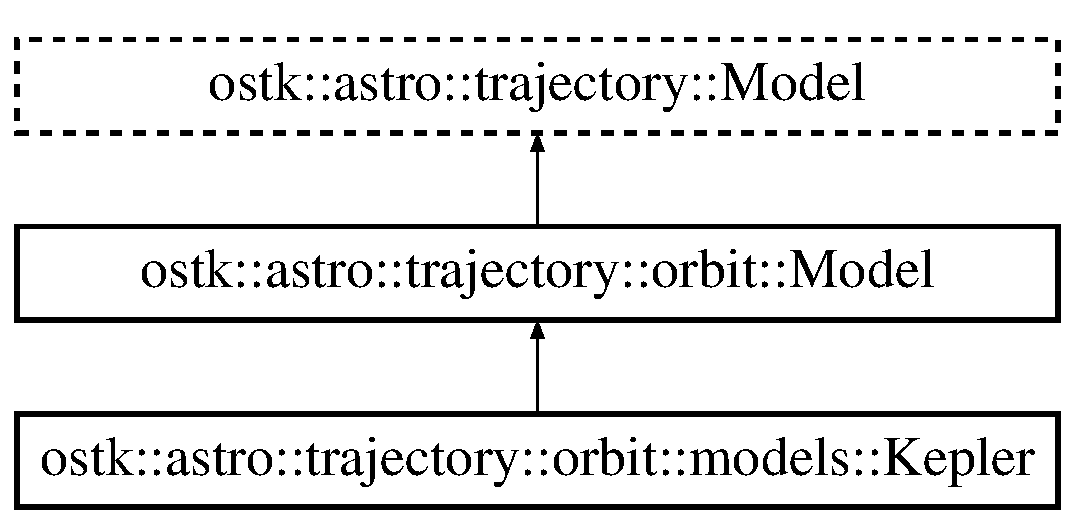
\includegraphics[height=3.000000cm]{classostk_1_1astro_1_1trajectory_1_1orbit_1_1models_1_1_kepler}
\end{center}
\end{figure}
\doxysubsection*{Public Types}
\begin{DoxyCompactItemize}
\item 
enum \mbox{\hyperlink{classostk_1_1astro_1_1trajectory_1_1orbit_1_1models_1_1_kepler_a3750f9177ff06a1938826e2c2881d5a9}{Perturbation\+Type}} \{ \mbox{\hyperlink{classostk_1_1astro_1_1trajectory_1_1orbit_1_1models_1_1_kepler_a3750f9177ff06a1938826e2c2881d5a9a6adf97f83acf6453d4a6a4b1070f3754}{Perturbation\+Type\+::\+None}}, 
\mbox{\hyperlink{classostk_1_1astro_1_1trajectory_1_1orbit_1_1models_1_1_kepler_a3750f9177ff06a1938826e2c2881d5a9a7f132d501fb9863844ab51697900d494}{Perturbation\+Type\+::\+J2}}, 
\mbox{\hyperlink{classostk_1_1astro_1_1trajectory_1_1orbit_1_1models_1_1_kepler_a3750f9177ff06a1938826e2c2881d5a9a0bf8a9e67aadee231938cadd6e85d369}{Perturbation\+Type\+::\+J4}}
 \}
\end{DoxyCompactItemize}
\doxysubsection*{Public Member Functions}
\begin{DoxyCompactItemize}
\item 
\mbox{\hyperlink{classostk_1_1astro_1_1trajectory_1_1orbit_1_1models_1_1_kepler_aebd9792c0965b4539a553afad07aff7a}{Kepler}} (const \mbox{\hyperlink{classostk_1_1astro_1_1trajectory_1_1orbit_1_1models_1_1kepler_1_1_c_o_e}{C\+OE}} \&a\+Classical\+Orbital\+Element\+Set, const Instant \&an\+Epoch, const Derived \&a\+Gravitational\+Parameter, const Length \&an\+Equatorial\+Radius, const Real \&a\+J2, const Real \&a\+J4, const \mbox{\hyperlink{classostk_1_1astro_1_1trajectory_1_1orbit_1_1models_1_1_kepler_a3750f9177ff06a1938826e2c2881d5a9}{Kepler\+::\+Perturbation\+Type}} \&a\+Perturbation\+Type)
\item 
\mbox{\hyperlink{classostk_1_1astro_1_1trajectory_1_1orbit_1_1models_1_1_kepler_af91d91131679176d920c658facaab07c}{Kepler}} (const \mbox{\hyperlink{classostk_1_1astro_1_1trajectory_1_1orbit_1_1models_1_1kepler_1_1_c_o_e}{C\+OE}} \&a\+Classical\+Orbital\+Element\+Set, const Instant \&an\+Epoch, const Celestial \&a\+Celestial\+Object, const \mbox{\hyperlink{classostk_1_1astro_1_1trajectory_1_1orbit_1_1models_1_1_kepler_a3750f9177ff06a1938826e2c2881d5a9}{Kepler\+::\+Perturbation\+Type}} \&a\+Perturbation\+Type, const bool in\+Fixed\+Frame=\mbox{\hyperlink{_kepler_8hpp_a42fbab7c9532a311984a768a10f815aa}{D\+E\+F\+A\+U\+L\+T\+\_\+\+I\+N\+\_\+\+F\+I\+X\+E\+D\+\_\+\+F\+R\+A\+ME}})
\item 
virtual \mbox{\hyperlink{classostk_1_1astro_1_1trajectory_1_1orbit_1_1models_1_1_kepler}{Kepler}} $\ast$ \mbox{\hyperlink{classostk_1_1astro_1_1trajectory_1_1orbit_1_1models_1_1_kepler_afb76b3571c73fb5c87129033f7d66520}{clone}} () const override
\item 
bool \mbox{\hyperlink{classostk_1_1astro_1_1trajectory_1_1orbit_1_1models_1_1_kepler_a0fa60d97287b75564e1e5a2390f137f4}{operator==}} (const \mbox{\hyperlink{classostk_1_1astro_1_1trajectory_1_1orbit_1_1models_1_1_kepler}{Kepler}} \&a\+Keplerian\+Model) const
\item 
bool \mbox{\hyperlink{classostk_1_1astro_1_1trajectory_1_1orbit_1_1models_1_1_kepler_aac43844f43000a181bf504529763bc82}{operator!=}} (const \mbox{\hyperlink{classostk_1_1astro_1_1trajectory_1_1orbit_1_1models_1_1_kepler}{Kepler}} \&a\+Keplerian\+Model) const
\item 
virtual bool \mbox{\hyperlink{classostk_1_1astro_1_1trajectory_1_1orbit_1_1models_1_1_kepler_a4c74402d5483a51e5e0fe1920cd52ec4}{is\+Defined}} () const override
\item 
\mbox{\hyperlink{classostk_1_1astro_1_1trajectory_1_1orbit_1_1models_1_1kepler_1_1_c_o_e}{C\+OE}} \mbox{\hyperlink{classostk_1_1astro_1_1trajectory_1_1orbit_1_1models_1_1_kepler_a1a5e2d4a27c4e20d91924a3a751cbba4}{get\+Classical\+Orbital\+Elements}} () const
\item 
virtual Instant \mbox{\hyperlink{classostk_1_1astro_1_1trajectory_1_1orbit_1_1models_1_1_kepler_a01551fd006896966d4d5e4442c182f92}{get\+Epoch}} () const override
\item 
virtual Integer \mbox{\hyperlink{classostk_1_1astro_1_1trajectory_1_1orbit_1_1models_1_1_kepler_a2aa5b94462f65ea7e703d319d3e028b3}{get\+Revolution\+Number\+At\+Epoch}} () const override
\item 
Derived \mbox{\hyperlink{classostk_1_1astro_1_1trajectory_1_1orbit_1_1models_1_1_kepler_af7e879bf88e9a388c86d836ac50d6a97}{get\+Gravitational\+Parameter}} () const
\item 
Length \mbox{\hyperlink{classostk_1_1astro_1_1trajectory_1_1orbit_1_1models_1_1_kepler_abd9cabfcb1a39b627d2809d3cb11dad8}{get\+Equatorial\+Radius}} () const
\item 
Real \mbox{\hyperlink{classostk_1_1astro_1_1trajectory_1_1orbit_1_1models_1_1_kepler_aeff5940802c7795d9d709a0fdf15fa64}{get\+J2}} () const
\item 
Real \mbox{\hyperlink{classostk_1_1astro_1_1trajectory_1_1orbit_1_1models_1_1_kepler_a15e3600757f990a833910dc54c389462}{get\+J4}} () const
\item 
\mbox{\hyperlink{classostk_1_1astro_1_1trajectory_1_1orbit_1_1models_1_1_kepler_a3750f9177ff06a1938826e2c2881d5a9}{Kepler\+::\+Perturbation\+Type}} \mbox{\hyperlink{classostk_1_1astro_1_1trajectory_1_1orbit_1_1models_1_1_kepler_a8f6d00fe11481e9267aded6f9aeafb1a}{get\+Perturbation\+Type}} () const
\item 
virtual \mbox{\hyperlink{classostk_1_1astro_1_1trajectory_1_1_state}{State}} \mbox{\hyperlink{classostk_1_1astro_1_1trajectory_1_1orbit_1_1models_1_1_kepler_a4de0c3d7a2b37c1c2ab4d6e207339809}{calculate\+State\+At}} (const Instant \&an\+Instant) const override
\item 
virtual Integer \mbox{\hyperlink{classostk_1_1astro_1_1trajectory_1_1orbit_1_1models_1_1_kepler_a312fe4296eadcb00799ce9981b0c4f18}{calculate\+Revolution\+Number\+At}} (const Instant \&an\+Instant) const override
\item 
virtual void \mbox{\hyperlink{classostk_1_1astro_1_1trajectory_1_1orbit_1_1models_1_1_kepler_a9c71803234f356ade03453e3ae19ae94}{print}} (std\+::ostream \&an\+Output\+Stream, bool display\+Decorator=true) const override
\end{DoxyCompactItemize}
\doxysubsection*{Static Public Member Functions}
\begin{DoxyCompactItemize}
\item 
static String \mbox{\hyperlink{classostk_1_1astro_1_1trajectory_1_1orbit_1_1models_1_1_kepler_ad780ed9b53e355ebef1597f86d30cf84}{String\+From\+Perturbation\+Type}} (const \mbox{\hyperlink{classostk_1_1astro_1_1trajectory_1_1orbit_1_1models_1_1_kepler_a3750f9177ff06a1938826e2c2881d5a9}{Kepler\+::\+Perturbation\+Type}} \&a\+Perturbation\+Type)
\end{DoxyCompactItemize}
\doxysubsection*{Protected Member Functions}
\begin{DoxyCompactItemize}
\item 
virtual bool \mbox{\hyperlink{classostk_1_1astro_1_1trajectory_1_1orbit_1_1models_1_1_kepler_ad2a61eb0cbd9887fc2180dc0818c209e}{operator==}} (const \mbox{\hyperlink{classostk_1_1astro_1_1trajectory_1_1_model}{trajectory\+::\+Model}} \&a\+Model) const override
\item 
virtual bool \mbox{\hyperlink{classostk_1_1astro_1_1trajectory_1_1orbit_1_1models_1_1_kepler_ab343575a423c5cecea4b21fa79c80726}{operator!=}} (const \mbox{\hyperlink{classostk_1_1astro_1_1trajectory_1_1_model}{trajectory\+::\+Model}} \&a\+Model) const override
\end{DoxyCompactItemize}
\doxysubsection*{Friends}
\begin{DoxyCompactItemize}
\item 
std\+::ostream \& \mbox{\hyperlink{classostk_1_1astro_1_1trajectory_1_1orbit_1_1models_1_1_kepler_aedb386ce32716dfb187f89b52b023f2b}{operator$<$$<$}} (std\+::ostream \&an\+Output\+Stream, const \mbox{\hyperlink{classostk_1_1astro_1_1trajectory_1_1orbit_1_1models_1_1_kepler}{Kepler}} \&a\+Keplerian\+Model)
\end{DoxyCompactItemize}


\doxysubsection{Member Enumeration Documentation}
\mbox{\Hypertarget{classostk_1_1astro_1_1trajectory_1_1orbit_1_1models_1_1_kepler_a3750f9177ff06a1938826e2c2881d5a9}\label{classostk_1_1astro_1_1trajectory_1_1orbit_1_1models_1_1_kepler_a3750f9177ff06a1938826e2c2881d5a9}} 
\index{ostk::astro::trajectory::orbit::models::Kepler@{ostk::astro::trajectory::orbit::models::Kepler}!PerturbationType@{PerturbationType}}
\index{PerturbationType@{PerturbationType}!ostk::astro::trajectory::orbit::models::Kepler@{ostk::astro::trajectory::orbit::models::Kepler}}
\doxysubsubsection{\texorpdfstring{PerturbationType}{PerturbationType}}
{\footnotesize\ttfamily enum \mbox{\hyperlink{classostk_1_1astro_1_1trajectory_1_1orbit_1_1models_1_1_kepler_a3750f9177ff06a1938826e2c2881d5a9}{ostk\+::astro\+::trajectory\+::orbit\+::models\+::\+Kepler\+::\+Perturbation\+Type}}\hspace{0.3cm}{\ttfamily [strong]}}

\begin{DoxyEnumFields}{Enumerator}
\raisebox{\heightof{T}}[0pt][0pt]{\index{None@{None}!ostk::astro::trajectory::orbit::models::Kepler@{ostk::astro::trajectory::orbit::models::Kepler}}\index{ostk::astro::trajectory::orbit::models::Kepler@{ostk::astro::trajectory::orbit::models::Kepler}!None@{None}}}\mbox{\Hypertarget{classostk_1_1astro_1_1trajectory_1_1orbit_1_1models_1_1_kepler_a3750f9177ff06a1938826e2c2881d5a9a6adf97f83acf6453d4a6a4b1070f3754}\label{classostk_1_1astro_1_1trajectory_1_1orbit_1_1models_1_1_kepler_a3750f9177ff06a1938826e2c2881d5a9a6adf97f83acf6453d4a6a4b1070f3754}} 
None&\\
\hline

\raisebox{\heightof{T}}[0pt][0pt]{\index{J2@{J2}!ostk::astro::trajectory::orbit::models::Kepler@{ostk::astro::trajectory::orbit::models::Kepler}}\index{ostk::astro::trajectory::orbit::models::Kepler@{ostk::astro::trajectory::orbit::models::Kepler}!J2@{J2}}}\mbox{\Hypertarget{classostk_1_1astro_1_1trajectory_1_1orbit_1_1models_1_1_kepler_a3750f9177ff06a1938826e2c2881d5a9a7f132d501fb9863844ab51697900d494}\label{classostk_1_1astro_1_1trajectory_1_1orbit_1_1models_1_1_kepler_a3750f9177ff06a1938826e2c2881d5a9a7f132d501fb9863844ab51697900d494}} 
J2&\\
\hline

\raisebox{\heightof{T}}[0pt][0pt]{\index{J4@{J4}!ostk::astro::trajectory::orbit::models::Kepler@{ostk::astro::trajectory::orbit::models::Kepler}}\index{ostk::astro::trajectory::orbit::models::Kepler@{ostk::astro::trajectory::orbit::models::Kepler}!J4@{J4}}}\mbox{\Hypertarget{classostk_1_1astro_1_1trajectory_1_1orbit_1_1models_1_1_kepler_a3750f9177ff06a1938826e2c2881d5a9a0bf8a9e67aadee231938cadd6e85d369}\label{classostk_1_1astro_1_1trajectory_1_1orbit_1_1models_1_1_kepler_a3750f9177ff06a1938826e2c2881d5a9a0bf8a9e67aadee231938cadd6e85d369}} 
J4&\\
\hline

\end{DoxyEnumFields}


\doxysubsection{Constructor \& Destructor Documentation}
\mbox{\Hypertarget{classostk_1_1astro_1_1trajectory_1_1orbit_1_1models_1_1_kepler_aebd9792c0965b4539a553afad07aff7a}\label{classostk_1_1astro_1_1trajectory_1_1orbit_1_1models_1_1_kepler_aebd9792c0965b4539a553afad07aff7a}} 
\index{ostk::astro::trajectory::orbit::models::Kepler@{ostk::astro::trajectory::orbit::models::Kepler}!Kepler@{Kepler}}
\index{Kepler@{Kepler}!ostk::astro::trajectory::orbit::models::Kepler@{ostk::astro::trajectory::orbit::models::Kepler}}
\doxysubsubsection{\texorpdfstring{Kepler()}{Kepler()}\hspace{0.1cm}{\footnotesize\ttfamily [1/2]}}
{\footnotesize\ttfamily ostk\+::astro\+::trajectory\+::orbit\+::models\+::\+Kepler\+::\+Kepler (\begin{DoxyParamCaption}\item[{const \mbox{\hyperlink{classostk_1_1astro_1_1trajectory_1_1orbit_1_1models_1_1kepler_1_1_c_o_e}{C\+OE}} \&}]{a\+Classical\+Orbital\+Element\+Set,  }\item[{const Instant \&}]{an\+Epoch,  }\item[{const Derived \&}]{a\+Gravitational\+Parameter,  }\item[{const Length \&}]{an\+Equatorial\+Radius,  }\item[{const Real \&}]{a\+J2,  }\item[{const Real \&}]{a\+J4,  }\item[{const \mbox{\hyperlink{classostk_1_1astro_1_1trajectory_1_1orbit_1_1models_1_1_kepler_a3750f9177ff06a1938826e2c2881d5a9}{Kepler\+::\+Perturbation\+Type}} \&}]{a\+Perturbation\+Type }\end{DoxyParamCaption})}

\mbox{\Hypertarget{classostk_1_1astro_1_1trajectory_1_1orbit_1_1models_1_1_kepler_af91d91131679176d920c658facaab07c}\label{classostk_1_1astro_1_1trajectory_1_1orbit_1_1models_1_1_kepler_af91d91131679176d920c658facaab07c}} 
\index{ostk::astro::trajectory::orbit::models::Kepler@{ostk::astro::trajectory::orbit::models::Kepler}!Kepler@{Kepler}}
\index{Kepler@{Kepler}!ostk::astro::trajectory::orbit::models::Kepler@{ostk::astro::trajectory::orbit::models::Kepler}}
\doxysubsubsection{\texorpdfstring{Kepler()}{Kepler()}\hspace{0.1cm}{\footnotesize\ttfamily [2/2]}}
{\footnotesize\ttfamily ostk\+::astro\+::trajectory\+::orbit\+::models\+::\+Kepler\+::\+Kepler (\begin{DoxyParamCaption}\item[{const \mbox{\hyperlink{classostk_1_1astro_1_1trajectory_1_1orbit_1_1models_1_1kepler_1_1_c_o_e}{C\+OE}} \&}]{a\+Classical\+Orbital\+Element\+Set,  }\item[{const Instant \&}]{an\+Epoch,  }\item[{const Celestial \&}]{a\+Celestial\+Object,  }\item[{const \mbox{\hyperlink{classostk_1_1astro_1_1trajectory_1_1orbit_1_1models_1_1_kepler_a3750f9177ff06a1938826e2c2881d5a9}{Kepler\+::\+Perturbation\+Type}} \&}]{a\+Perturbation\+Type,  }\item[{const bool}]{in\+Fixed\+Frame = {\ttfamily \mbox{\hyperlink{_kepler_8hpp_a42fbab7c9532a311984a768a10f815aa}{D\+E\+F\+A\+U\+L\+T\+\_\+\+I\+N\+\_\+\+F\+I\+X\+E\+D\+\_\+\+F\+R\+A\+ME}}} }\end{DoxyParamCaption})}



\doxysubsection{Member Function Documentation}
\mbox{\Hypertarget{classostk_1_1astro_1_1trajectory_1_1orbit_1_1models_1_1_kepler_a312fe4296eadcb00799ce9981b0c4f18}\label{classostk_1_1astro_1_1trajectory_1_1orbit_1_1models_1_1_kepler_a312fe4296eadcb00799ce9981b0c4f18}} 
\index{ostk::astro::trajectory::orbit::models::Kepler@{ostk::astro::trajectory::orbit::models::Kepler}!calculateRevolutionNumberAt@{calculateRevolutionNumberAt}}
\index{calculateRevolutionNumberAt@{calculateRevolutionNumberAt}!ostk::astro::trajectory::orbit::models::Kepler@{ostk::astro::trajectory::orbit::models::Kepler}}
\doxysubsubsection{\texorpdfstring{calculateRevolutionNumberAt()}{calculateRevolutionNumberAt()}}
{\footnotesize\ttfamily Integer ostk\+::astro\+::trajectory\+::orbit\+::models\+::\+Kepler\+::calculate\+Revolution\+Number\+At (\begin{DoxyParamCaption}\item[{const Instant \&}]{an\+Instant }\end{DoxyParamCaption}) const\hspace{0.3cm}{\ttfamily [override]}, {\ttfamily [virtual]}}



Implements \mbox{\hyperlink{classostk_1_1astro_1_1trajectory_1_1orbit_1_1_model_aeecf4cc22fa9c766801936c468cc52ac}{ostk\+::astro\+::trajectory\+::orbit\+::\+Model}}.

\mbox{\Hypertarget{classostk_1_1astro_1_1trajectory_1_1orbit_1_1models_1_1_kepler_a4de0c3d7a2b37c1c2ab4d6e207339809}\label{classostk_1_1astro_1_1trajectory_1_1orbit_1_1models_1_1_kepler_a4de0c3d7a2b37c1c2ab4d6e207339809}} 
\index{ostk::astro::trajectory::orbit::models::Kepler@{ostk::astro::trajectory::orbit::models::Kepler}!calculateStateAt@{calculateStateAt}}
\index{calculateStateAt@{calculateStateAt}!ostk::astro::trajectory::orbit::models::Kepler@{ostk::astro::trajectory::orbit::models::Kepler}}
\doxysubsubsection{\texorpdfstring{calculateStateAt()}{calculateStateAt()}}
{\footnotesize\ttfamily \mbox{\hyperlink{classostk_1_1astro_1_1trajectory_1_1_state}{State}} ostk\+::astro\+::trajectory\+::orbit\+::models\+::\+Kepler\+::calculate\+State\+At (\begin{DoxyParamCaption}\item[{const Instant \&}]{an\+Instant }\end{DoxyParamCaption}) const\hspace{0.3cm}{\ttfamily [override]}, {\ttfamily [virtual]}}



Implements \mbox{\hyperlink{classostk_1_1astro_1_1trajectory_1_1orbit_1_1_model_a34a0d8979ec1f7ade3e434fc0dad3711}{ostk\+::astro\+::trajectory\+::orbit\+::\+Model}}.

\mbox{\Hypertarget{classostk_1_1astro_1_1trajectory_1_1orbit_1_1models_1_1_kepler_afb76b3571c73fb5c87129033f7d66520}\label{classostk_1_1astro_1_1trajectory_1_1orbit_1_1models_1_1_kepler_afb76b3571c73fb5c87129033f7d66520}} 
\index{ostk::astro::trajectory::orbit::models::Kepler@{ostk::astro::trajectory::orbit::models::Kepler}!clone@{clone}}
\index{clone@{clone}!ostk::astro::trajectory::orbit::models::Kepler@{ostk::astro::trajectory::orbit::models::Kepler}}
\doxysubsubsection{\texorpdfstring{clone()}{clone()}}
{\footnotesize\ttfamily \mbox{\hyperlink{classostk_1_1astro_1_1trajectory_1_1orbit_1_1models_1_1_kepler}{Kepler}} $\ast$ ostk\+::astro\+::trajectory\+::orbit\+::models\+::\+Kepler\+::clone (\begin{DoxyParamCaption}{ }\end{DoxyParamCaption}) const\hspace{0.3cm}{\ttfamily [override]}, {\ttfamily [virtual]}}



Implements \mbox{\hyperlink{classostk_1_1astro_1_1trajectory_1_1orbit_1_1_model_a53dc07564e4c7c444da46360aa8ada15}{ostk\+::astro\+::trajectory\+::orbit\+::\+Model}}.

\mbox{\Hypertarget{classostk_1_1astro_1_1trajectory_1_1orbit_1_1models_1_1_kepler_a1a5e2d4a27c4e20d91924a3a751cbba4}\label{classostk_1_1astro_1_1trajectory_1_1orbit_1_1models_1_1_kepler_a1a5e2d4a27c4e20d91924a3a751cbba4}} 
\index{ostk::astro::trajectory::orbit::models::Kepler@{ostk::astro::trajectory::orbit::models::Kepler}!getClassicalOrbitalElements@{getClassicalOrbitalElements}}
\index{getClassicalOrbitalElements@{getClassicalOrbitalElements}!ostk::astro::trajectory::orbit::models::Kepler@{ostk::astro::trajectory::orbit::models::Kepler}}
\doxysubsubsection{\texorpdfstring{getClassicalOrbitalElements()}{getClassicalOrbitalElements()}}
{\footnotesize\ttfamily \mbox{\hyperlink{classostk_1_1astro_1_1trajectory_1_1orbit_1_1models_1_1kepler_1_1_c_o_e}{C\+OE}} ostk\+::astro\+::trajectory\+::orbit\+::models\+::\+Kepler\+::get\+Classical\+Orbital\+Elements (\begin{DoxyParamCaption}{ }\end{DoxyParamCaption}) const}

\mbox{\Hypertarget{classostk_1_1astro_1_1trajectory_1_1orbit_1_1models_1_1_kepler_a01551fd006896966d4d5e4442c182f92}\label{classostk_1_1astro_1_1trajectory_1_1orbit_1_1models_1_1_kepler_a01551fd006896966d4d5e4442c182f92}} 
\index{ostk::astro::trajectory::orbit::models::Kepler@{ostk::astro::trajectory::orbit::models::Kepler}!getEpoch@{getEpoch}}
\index{getEpoch@{getEpoch}!ostk::astro::trajectory::orbit::models::Kepler@{ostk::astro::trajectory::orbit::models::Kepler}}
\doxysubsubsection{\texorpdfstring{getEpoch()}{getEpoch()}}
{\footnotesize\ttfamily Instant ostk\+::astro\+::trajectory\+::orbit\+::models\+::\+Kepler\+::get\+Epoch (\begin{DoxyParamCaption}{ }\end{DoxyParamCaption}) const\hspace{0.3cm}{\ttfamily [override]}, {\ttfamily [virtual]}}



Implements \mbox{\hyperlink{classostk_1_1astro_1_1trajectory_1_1orbit_1_1_model_a22055d5ab4c22e6177a3ddb8f45f1f9b}{ostk\+::astro\+::trajectory\+::orbit\+::\+Model}}.

\mbox{\Hypertarget{classostk_1_1astro_1_1trajectory_1_1orbit_1_1models_1_1_kepler_abd9cabfcb1a39b627d2809d3cb11dad8}\label{classostk_1_1astro_1_1trajectory_1_1orbit_1_1models_1_1_kepler_abd9cabfcb1a39b627d2809d3cb11dad8}} 
\index{ostk::astro::trajectory::orbit::models::Kepler@{ostk::astro::trajectory::orbit::models::Kepler}!getEquatorialRadius@{getEquatorialRadius}}
\index{getEquatorialRadius@{getEquatorialRadius}!ostk::astro::trajectory::orbit::models::Kepler@{ostk::astro::trajectory::orbit::models::Kepler}}
\doxysubsubsection{\texorpdfstring{getEquatorialRadius()}{getEquatorialRadius()}}
{\footnotesize\ttfamily Length ostk\+::astro\+::trajectory\+::orbit\+::models\+::\+Kepler\+::get\+Equatorial\+Radius (\begin{DoxyParamCaption}{ }\end{DoxyParamCaption}) const}

\mbox{\Hypertarget{classostk_1_1astro_1_1trajectory_1_1orbit_1_1models_1_1_kepler_af7e879bf88e9a388c86d836ac50d6a97}\label{classostk_1_1astro_1_1trajectory_1_1orbit_1_1models_1_1_kepler_af7e879bf88e9a388c86d836ac50d6a97}} 
\index{ostk::astro::trajectory::orbit::models::Kepler@{ostk::astro::trajectory::orbit::models::Kepler}!getGravitationalParameter@{getGravitationalParameter}}
\index{getGravitationalParameter@{getGravitationalParameter}!ostk::astro::trajectory::orbit::models::Kepler@{ostk::astro::trajectory::orbit::models::Kepler}}
\doxysubsubsection{\texorpdfstring{getGravitationalParameter()}{getGravitationalParameter()}}
{\footnotesize\ttfamily Derived ostk\+::astro\+::trajectory\+::orbit\+::models\+::\+Kepler\+::get\+Gravitational\+Parameter (\begin{DoxyParamCaption}{ }\end{DoxyParamCaption}) const}

\mbox{\Hypertarget{classostk_1_1astro_1_1trajectory_1_1orbit_1_1models_1_1_kepler_aeff5940802c7795d9d709a0fdf15fa64}\label{classostk_1_1astro_1_1trajectory_1_1orbit_1_1models_1_1_kepler_aeff5940802c7795d9d709a0fdf15fa64}} 
\index{ostk::astro::trajectory::orbit::models::Kepler@{ostk::astro::trajectory::orbit::models::Kepler}!getJ2@{getJ2}}
\index{getJ2@{getJ2}!ostk::astro::trajectory::orbit::models::Kepler@{ostk::astro::trajectory::orbit::models::Kepler}}
\doxysubsubsection{\texorpdfstring{getJ2()}{getJ2()}}
{\footnotesize\ttfamily Real ostk\+::astro\+::trajectory\+::orbit\+::models\+::\+Kepler\+::get\+J2 (\begin{DoxyParamCaption}{ }\end{DoxyParamCaption}) const}

\mbox{\Hypertarget{classostk_1_1astro_1_1trajectory_1_1orbit_1_1models_1_1_kepler_a15e3600757f990a833910dc54c389462}\label{classostk_1_1astro_1_1trajectory_1_1orbit_1_1models_1_1_kepler_a15e3600757f990a833910dc54c389462}} 
\index{ostk::astro::trajectory::orbit::models::Kepler@{ostk::astro::trajectory::orbit::models::Kepler}!getJ4@{getJ4}}
\index{getJ4@{getJ4}!ostk::astro::trajectory::orbit::models::Kepler@{ostk::astro::trajectory::orbit::models::Kepler}}
\doxysubsubsection{\texorpdfstring{getJ4()}{getJ4()}}
{\footnotesize\ttfamily Real ostk\+::astro\+::trajectory\+::orbit\+::models\+::\+Kepler\+::get\+J4 (\begin{DoxyParamCaption}{ }\end{DoxyParamCaption}) const}

\mbox{\Hypertarget{classostk_1_1astro_1_1trajectory_1_1orbit_1_1models_1_1_kepler_a8f6d00fe11481e9267aded6f9aeafb1a}\label{classostk_1_1astro_1_1trajectory_1_1orbit_1_1models_1_1_kepler_a8f6d00fe11481e9267aded6f9aeafb1a}} 
\index{ostk::astro::trajectory::orbit::models::Kepler@{ostk::astro::trajectory::orbit::models::Kepler}!getPerturbationType@{getPerturbationType}}
\index{getPerturbationType@{getPerturbationType}!ostk::astro::trajectory::orbit::models::Kepler@{ostk::astro::trajectory::orbit::models::Kepler}}
\doxysubsubsection{\texorpdfstring{getPerturbationType()}{getPerturbationType()}}
{\footnotesize\ttfamily \mbox{\hyperlink{classostk_1_1astro_1_1trajectory_1_1orbit_1_1models_1_1_kepler_a3750f9177ff06a1938826e2c2881d5a9}{Kepler\+::\+Perturbation\+Type}} ostk\+::astro\+::trajectory\+::orbit\+::models\+::\+Kepler\+::get\+Perturbation\+Type (\begin{DoxyParamCaption}{ }\end{DoxyParamCaption}) const}

\mbox{\Hypertarget{classostk_1_1astro_1_1trajectory_1_1orbit_1_1models_1_1_kepler_a2aa5b94462f65ea7e703d319d3e028b3}\label{classostk_1_1astro_1_1trajectory_1_1orbit_1_1models_1_1_kepler_a2aa5b94462f65ea7e703d319d3e028b3}} 
\index{ostk::astro::trajectory::orbit::models::Kepler@{ostk::astro::trajectory::orbit::models::Kepler}!getRevolutionNumberAtEpoch@{getRevolutionNumberAtEpoch}}
\index{getRevolutionNumberAtEpoch@{getRevolutionNumberAtEpoch}!ostk::astro::trajectory::orbit::models::Kepler@{ostk::astro::trajectory::orbit::models::Kepler}}
\doxysubsubsection{\texorpdfstring{getRevolutionNumberAtEpoch()}{getRevolutionNumberAtEpoch()}}
{\footnotesize\ttfamily Integer ostk\+::astro\+::trajectory\+::orbit\+::models\+::\+Kepler\+::get\+Revolution\+Number\+At\+Epoch (\begin{DoxyParamCaption}{ }\end{DoxyParamCaption}) const\hspace{0.3cm}{\ttfamily [override]}, {\ttfamily [virtual]}}



Implements \mbox{\hyperlink{classostk_1_1astro_1_1trajectory_1_1orbit_1_1_model_af3f1866f86045da2c05efe4165735cf4}{ostk\+::astro\+::trajectory\+::orbit\+::\+Model}}.

\mbox{\Hypertarget{classostk_1_1astro_1_1trajectory_1_1orbit_1_1models_1_1_kepler_a4c74402d5483a51e5e0fe1920cd52ec4}\label{classostk_1_1astro_1_1trajectory_1_1orbit_1_1models_1_1_kepler_a4c74402d5483a51e5e0fe1920cd52ec4}} 
\index{ostk::astro::trajectory::orbit::models::Kepler@{ostk::astro::trajectory::orbit::models::Kepler}!isDefined@{isDefined}}
\index{isDefined@{isDefined}!ostk::astro::trajectory::orbit::models::Kepler@{ostk::astro::trajectory::orbit::models::Kepler}}
\doxysubsubsection{\texorpdfstring{isDefined()}{isDefined()}}
{\footnotesize\ttfamily bool ostk\+::astro\+::trajectory\+::orbit\+::models\+::\+Kepler\+::is\+Defined (\begin{DoxyParamCaption}{ }\end{DoxyParamCaption}) const\hspace{0.3cm}{\ttfamily [override]}, {\ttfamily [virtual]}}



Implements \mbox{\hyperlink{classostk_1_1astro_1_1trajectory_1_1orbit_1_1_model_a13c5b5693dd86a072da0bd0e319bacc2}{ostk\+::astro\+::trajectory\+::orbit\+::\+Model}}.

\mbox{\Hypertarget{classostk_1_1astro_1_1trajectory_1_1orbit_1_1models_1_1_kepler_aac43844f43000a181bf504529763bc82}\label{classostk_1_1astro_1_1trajectory_1_1orbit_1_1models_1_1_kepler_aac43844f43000a181bf504529763bc82}} 
\index{ostk::astro::trajectory::orbit::models::Kepler@{ostk::astro::trajectory::orbit::models::Kepler}!operator"!=@{operator"!=}}
\index{operator"!=@{operator"!=}!ostk::astro::trajectory::orbit::models::Kepler@{ostk::astro::trajectory::orbit::models::Kepler}}
\doxysubsubsection{\texorpdfstring{operator"!=()}{operator!=()}\hspace{0.1cm}{\footnotesize\ttfamily [1/2]}}
{\footnotesize\ttfamily bool ostk\+::astro\+::trajectory\+::orbit\+::models\+::\+Kepler\+::operator!= (\begin{DoxyParamCaption}\item[{const \mbox{\hyperlink{classostk_1_1astro_1_1trajectory_1_1orbit_1_1models_1_1_kepler}{Kepler}} \&}]{a\+Keplerian\+Model }\end{DoxyParamCaption}) const}

\mbox{\Hypertarget{classostk_1_1astro_1_1trajectory_1_1orbit_1_1models_1_1_kepler_ab343575a423c5cecea4b21fa79c80726}\label{classostk_1_1astro_1_1trajectory_1_1orbit_1_1models_1_1_kepler_ab343575a423c5cecea4b21fa79c80726}} 
\index{ostk::astro::trajectory::orbit::models::Kepler@{ostk::astro::trajectory::orbit::models::Kepler}!operator"!=@{operator"!=}}
\index{operator"!=@{operator"!=}!ostk::astro::trajectory::orbit::models::Kepler@{ostk::astro::trajectory::orbit::models::Kepler}}
\doxysubsubsection{\texorpdfstring{operator"!=()}{operator!=()}\hspace{0.1cm}{\footnotesize\ttfamily [2/2]}}
{\footnotesize\ttfamily bool ostk\+::astro\+::trajectory\+::orbit\+::models\+::\+Kepler\+::operator!= (\begin{DoxyParamCaption}\item[{const \mbox{\hyperlink{classostk_1_1astro_1_1trajectory_1_1_model}{trajectory\+::\+Model}} \&}]{a\+Model }\end{DoxyParamCaption}) const\hspace{0.3cm}{\ttfamily [override]}, {\ttfamily [protected]}, {\ttfamily [virtual]}}



Implements \mbox{\hyperlink{classostk_1_1astro_1_1trajectory_1_1_model_a2dd77b9f6939d738f3a489f26c955340}{ostk\+::astro\+::trajectory\+::\+Model}}.

\mbox{\Hypertarget{classostk_1_1astro_1_1trajectory_1_1orbit_1_1models_1_1_kepler_a0fa60d97287b75564e1e5a2390f137f4}\label{classostk_1_1astro_1_1trajectory_1_1orbit_1_1models_1_1_kepler_a0fa60d97287b75564e1e5a2390f137f4}} 
\index{ostk::astro::trajectory::orbit::models::Kepler@{ostk::astro::trajectory::orbit::models::Kepler}!operator==@{operator==}}
\index{operator==@{operator==}!ostk::astro::trajectory::orbit::models::Kepler@{ostk::astro::trajectory::orbit::models::Kepler}}
\doxysubsubsection{\texorpdfstring{operator==()}{operator==()}\hspace{0.1cm}{\footnotesize\ttfamily [1/2]}}
{\footnotesize\ttfamily bool ostk\+::astro\+::trajectory\+::orbit\+::models\+::\+Kepler\+::operator== (\begin{DoxyParamCaption}\item[{const \mbox{\hyperlink{classostk_1_1astro_1_1trajectory_1_1orbit_1_1models_1_1_kepler}{Kepler}} \&}]{a\+Keplerian\+Model }\end{DoxyParamCaption}) const}

\mbox{\Hypertarget{classostk_1_1astro_1_1trajectory_1_1orbit_1_1models_1_1_kepler_ad2a61eb0cbd9887fc2180dc0818c209e}\label{classostk_1_1astro_1_1trajectory_1_1orbit_1_1models_1_1_kepler_ad2a61eb0cbd9887fc2180dc0818c209e}} 
\index{ostk::astro::trajectory::orbit::models::Kepler@{ostk::astro::trajectory::orbit::models::Kepler}!operator==@{operator==}}
\index{operator==@{operator==}!ostk::astro::trajectory::orbit::models::Kepler@{ostk::astro::trajectory::orbit::models::Kepler}}
\doxysubsubsection{\texorpdfstring{operator==()}{operator==()}\hspace{0.1cm}{\footnotesize\ttfamily [2/2]}}
{\footnotesize\ttfamily bool ostk\+::astro\+::trajectory\+::orbit\+::models\+::\+Kepler\+::operator== (\begin{DoxyParamCaption}\item[{const \mbox{\hyperlink{classostk_1_1astro_1_1trajectory_1_1_model}{trajectory\+::\+Model}} \&}]{a\+Model }\end{DoxyParamCaption}) const\hspace{0.3cm}{\ttfamily [override]}, {\ttfamily [protected]}, {\ttfamily [virtual]}}



Implements \mbox{\hyperlink{classostk_1_1astro_1_1trajectory_1_1_model_a874f79846e845859c070ce1b9874fc9c}{ostk\+::astro\+::trajectory\+::\+Model}}.

\mbox{\Hypertarget{classostk_1_1astro_1_1trajectory_1_1orbit_1_1models_1_1_kepler_a9c71803234f356ade03453e3ae19ae94}\label{classostk_1_1astro_1_1trajectory_1_1orbit_1_1models_1_1_kepler_a9c71803234f356ade03453e3ae19ae94}} 
\index{ostk::astro::trajectory::orbit::models::Kepler@{ostk::astro::trajectory::orbit::models::Kepler}!print@{print}}
\index{print@{print}!ostk::astro::trajectory::orbit::models::Kepler@{ostk::astro::trajectory::orbit::models::Kepler}}
\doxysubsubsection{\texorpdfstring{print()}{print()}}
{\footnotesize\ttfamily void ostk\+::astro\+::trajectory\+::orbit\+::models\+::\+Kepler\+::print (\begin{DoxyParamCaption}\item[{std\+::ostream \&}]{an\+Output\+Stream,  }\item[{bool}]{display\+Decorator = {\ttfamily true} }\end{DoxyParamCaption}) const\hspace{0.3cm}{\ttfamily [override]}, {\ttfamily [virtual]}}



Implements \mbox{\hyperlink{classostk_1_1astro_1_1trajectory_1_1orbit_1_1_model_a8ea45c1a6e51a6153ce3f72f5294f0c6}{ostk\+::astro\+::trajectory\+::orbit\+::\+Model}}.

\mbox{\Hypertarget{classostk_1_1astro_1_1trajectory_1_1orbit_1_1models_1_1_kepler_ad780ed9b53e355ebef1597f86d30cf84}\label{classostk_1_1astro_1_1trajectory_1_1orbit_1_1models_1_1_kepler_ad780ed9b53e355ebef1597f86d30cf84}} 
\index{ostk::astro::trajectory::orbit::models::Kepler@{ostk::astro::trajectory::orbit::models::Kepler}!StringFromPerturbationType@{StringFromPerturbationType}}
\index{StringFromPerturbationType@{StringFromPerturbationType}!ostk::astro::trajectory::orbit::models::Kepler@{ostk::astro::trajectory::orbit::models::Kepler}}
\doxysubsubsection{\texorpdfstring{StringFromPerturbationType()}{StringFromPerturbationType()}}
{\footnotesize\ttfamily String ostk\+::astro\+::trajectory\+::orbit\+::models\+::\+Kepler\+::\+String\+From\+Perturbation\+Type (\begin{DoxyParamCaption}\item[{const \mbox{\hyperlink{classostk_1_1astro_1_1trajectory_1_1orbit_1_1models_1_1_kepler_a3750f9177ff06a1938826e2c2881d5a9}{Kepler\+::\+Perturbation\+Type}} \&}]{a\+Perturbation\+Type }\end{DoxyParamCaption})\hspace{0.3cm}{\ttfamily [static]}}



\doxysubsection{Friends And Related Function Documentation}
\mbox{\Hypertarget{classostk_1_1astro_1_1trajectory_1_1orbit_1_1models_1_1_kepler_aedb386ce32716dfb187f89b52b023f2b}\label{classostk_1_1astro_1_1trajectory_1_1orbit_1_1models_1_1_kepler_aedb386ce32716dfb187f89b52b023f2b}} 
\index{ostk::astro::trajectory::orbit::models::Kepler@{ostk::astro::trajectory::orbit::models::Kepler}!operator$<$$<$@{operator$<$$<$}}
\index{operator$<$$<$@{operator$<$$<$}!ostk::astro::trajectory::orbit::models::Kepler@{ostk::astro::trajectory::orbit::models::Kepler}}
\doxysubsubsection{\texorpdfstring{operator$<$$<$}{operator<<}}
{\footnotesize\ttfamily std\+::ostream\& operator$<$$<$ (\begin{DoxyParamCaption}\item[{std\+::ostream \&}]{an\+Output\+Stream,  }\item[{const \mbox{\hyperlink{classostk_1_1astro_1_1trajectory_1_1orbit_1_1models_1_1_kepler}{Kepler}} \&}]{a\+Keplerian\+Model }\end{DoxyParamCaption})\hspace{0.3cm}{\ttfamily [friend]}}



The documentation for this class was generated from the following files\+:\begin{DoxyCompactItemize}
\item 
include/\+Open\+Space\+Toolkit/\+Astrodynamics/\+Trajectory/\+Orbit/\+Models/\mbox{\hyperlink{_kepler_8hpp}{Kepler.\+hpp}}\item 
src/\+Open\+Space\+Toolkit/\+Astrodynamics/\+Trajectory/\+Orbit/\+Models/\mbox{\hyperlink{_kepler_8cpp}{Kepler.\+cpp}}\end{DoxyCompactItemize}

\hypertarget{structostk_1_1astro_1_1conjunction_1_1messages_1_1ccsds_1_1_c_d_m_1_1_metadata}{}\doxysection{ostk\+::astro\+::conjunction\+::messages\+::ccsds\+::C\+DM\+::Metadata Struct Reference}
\label{structostk_1_1astro_1_1conjunction_1_1messages_1_1ccsds_1_1_c_d_m_1_1_metadata}\index{ostk::astro::conjunction::messages::ccsds::CDM::Metadata@{ostk::astro::conjunction::messages::ccsds::CDM::Metadata}}


{\ttfamily \#include $<$C\+D\+M.\+hpp$>$}

\doxysubsection*{Public Attributes}
\begin{DoxyCompactItemize}
\item 
String \mbox{\hyperlink{structostk_1_1astro_1_1conjunction_1_1messages_1_1ccsds_1_1_c_d_m_1_1_metadata_a96b46dae4032dba90f24601425a8ace8}{comment}} = String\+::\+Empty()
\item 
String \mbox{\hyperlink{structostk_1_1astro_1_1conjunction_1_1messages_1_1ccsds_1_1_c_d_m_1_1_metadata_ace0fe39627c532a8b21a84c9c6886372}{object}}
\item 
Integer \mbox{\hyperlink{structostk_1_1astro_1_1conjunction_1_1messages_1_1ccsds_1_1_c_d_m_1_1_metadata_a135bbf761e45624d5cf29677756cce18}{object\+Designator}}
\item 
String \mbox{\hyperlink{structostk_1_1astro_1_1conjunction_1_1messages_1_1ccsds_1_1_c_d_m_1_1_metadata_a91b077a0f07ebf0c75816ad7f2fb4ba1}{catalog\+Name}}
\item 
String \mbox{\hyperlink{structostk_1_1astro_1_1conjunction_1_1messages_1_1ccsds_1_1_c_d_m_1_1_metadata_a842210f2ca1dacc597cfd570aa57c19d}{object\+Name}}
\item 
String \mbox{\hyperlink{structostk_1_1astro_1_1conjunction_1_1messages_1_1ccsds_1_1_c_d_m_1_1_metadata_ac11a59f1a624a5e7ada91a82b24bde2c}{international\+Designator}}
\item 
\mbox{\hyperlink{classostk_1_1astro_1_1conjunction_1_1messages_1_1ccsds_1_1_c_d_m_a9ef446f2327904fc0516249120ec9d71}{Object\+Type}} \mbox{\hyperlink{structostk_1_1astro_1_1conjunction_1_1messages_1_1ccsds_1_1_c_d_m_1_1_metadata_ace0a28e8456b7e950def75e9be2488da}{object\+Type}} = \mbox{\hyperlink{classostk_1_1astro_1_1conjunction_1_1messages_1_1ccsds_1_1_c_d_m_a9ef446f2327904fc0516249120ec9d71a88183b946cc5f0e8c96b2e66e1c74a7e}{Object\+Type\+::\+Unknown}}
\item 
String \mbox{\hyperlink{structostk_1_1astro_1_1conjunction_1_1messages_1_1ccsds_1_1_c_d_m_1_1_metadata_a6a891404a543cb582f1ea6289dc7bc59}{operator\+Contact\+Position}} = String\+::\+Empty()
\item 
String \mbox{\hyperlink{structostk_1_1astro_1_1conjunction_1_1messages_1_1ccsds_1_1_c_d_m_1_1_metadata_ada18b3efa3a6bb2df54ffc6f00cbbaaf}{operator\+Orgnization}} = String\+::\+Empty()
\item 
String \mbox{\hyperlink{structostk_1_1astro_1_1conjunction_1_1messages_1_1ccsds_1_1_c_d_m_1_1_metadata_a410654e822689ffb55db47df0ca8cbbf}{operator\+Phone}} = String\+::\+Empty()
\item 
String \mbox{\hyperlink{structostk_1_1astro_1_1conjunction_1_1messages_1_1ccsds_1_1_c_d_m_1_1_metadata_a0a577646ca9eb97424c29615f34ca477}{operator\+Email}} = String\+::\+Empty()
\item 
String \mbox{\hyperlink{structostk_1_1astro_1_1conjunction_1_1messages_1_1ccsds_1_1_c_d_m_1_1_metadata_a0c07d1d437162f4cb2c0e0ac9404e72c}{ephemeris\+Name}}
\item 
String \mbox{\hyperlink{structostk_1_1astro_1_1conjunction_1_1messages_1_1ccsds_1_1_c_d_m_1_1_metadata_aa75d6df4752331b1fdd080556fa602c6}{covariance\+Method}}
\item 
String \mbox{\hyperlink{structostk_1_1astro_1_1conjunction_1_1messages_1_1ccsds_1_1_c_d_m_1_1_metadata_af05d99ba66c816043e0fd1e25f050111}{maneuverable}}
\item 
String \mbox{\hyperlink{structostk_1_1astro_1_1conjunction_1_1messages_1_1ccsds_1_1_c_d_m_1_1_metadata_a850262b5d5528e0d4e871c747043f11f}{orbit\+Center}} = String\+::\+Empty()
\item 
String \mbox{\hyperlink{structostk_1_1astro_1_1conjunction_1_1messages_1_1ccsds_1_1_c_d_m_1_1_metadata_a1f7760be8ce00cf588146c557a7511b4}{ref\+Frame}}
\item 
String \mbox{\hyperlink{structostk_1_1astro_1_1conjunction_1_1messages_1_1ccsds_1_1_c_d_m_1_1_metadata_ac277170a570e49b737771b55005a9bb4}{gravity\+Model}} = String\+::\+Empty()
\item 
String \mbox{\hyperlink{structostk_1_1astro_1_1conjunction_1_1messages_1_1ccsds_1_1_c_d_m_1_1_metadata_a7c3419da001046c4d3b65072989dc563}{atmospheric\+Model}} = String\+::\+Empty()
\item 
String \mbox{\hyperlink{structostk_1_1astro_1_1conjunction_1_1messages_1_1ccsds_1_1_c_d_m_1_1_metadata_a938eed4b4146a7e02e24d37fb35d1e26}{n\+Body\+Perturbations}} = String\+::\+Empty()
\item 
bool \mbox{\hyperlink{structostk_1_1astro_1_1conjunction_1_1messages_1_1ccsds_1_1_c_d_m_1_1_metadata_a1f391661d25def1092b6051327e120cb}{solar\+Radiation\+Pressure}} = false
\item 
bool \mbox{\hyperlink{structostk_1_1astro_1_1conjunction_1_1messages_1_1ccsds_1_1_c_d_m_1_1_metadata_a059320ce7123670321382151ff465409}{earth\+Tides}} = false
\item 
bool \mbox{\hyperlink{structostk_1_1astro_1_1conjunction_1_1messages_1_1ccsds_1_1_c_d_m_1_1_metadata_ad5bded86c0fe3b4589f66c135d41016a}{in\+Track\+Thrust}} = false
\end{DoxyCompactItemize}


\doxysubsection{Member Data Documentation}
\mbox{\Hypertarget{structostk_1_1astro_1_1conjunction_1_1messages_1_1ccsds_1_1_c_d_m_1_1_metadata_a7c3419da001046c4d3b65072989dc563}\label{structostk_1_1astro_1_1conjunction_1_1messages_1_1ccsds_1_1_c_d_m_1_1_metadata_a7c3419da001046c4d3b65072989dc563}} 
\index{ostk::astro::conjunction::messages::ccsds::CDM::Metadata@{ostk::astro::conjunction::messages::ccsds::CDM::Metadata}!atmosphericModel@{atmosphericModel}}
\index{atmosphericModel@{atmosphericModel}!ostk::astro::conjunction::messages::ccsds::CDM::Metadata@{ostk::astro::conjunction::messages::ccsds::CDM::Metadata}}
\doxysubsubsection{\texorpdfstring{atmosphericModel}{atmosphericModel}}
{\footnotesize\ttfamily String ostk\+::astro\+::conjunction\+::messages\+::ccsds\+::\+C\+D\+M\+::\+Metadata\+::atmospheric\+Model = String\+::\+Empty()}

\mbox{\Hypertarget{structostk_1_1astro_1_1conjunction_1_1messages_1_1ccsds_1_1_c_d_m_1_1_metadata_a91b077a0f07ebf0c75816ad7f2fb4ba1}\label{structostk_1_1astro_1_1conjunction_1_1messages_1_1ccsds_1_1_c_d_m_1_1_metadata_a91b077a0f07ebf0c75816ad7f2fb4ba1}} 
\index{ostk::astro::conjunction::messages::ccsds::CDM::Metadata@{ostk::astro::conjunction::messages::ccsds::CDM::Metadata}!catalogName@{catalogName}}
\index{catalogName@{catalogName}!ostk::astro::conjunction::messages::ccsds::CDM::Metadata@{ostk::astro::conjunction::messages::ccsds::CDM::Metadata}}
\doxysubsubsection{\texorpdfstring{catalogName}{catalogName}}
{\footnotesize\ttfamily String ostk\+::astro\+::conjunction\+::messages\+::ccsds\+::\+C\+D\+M\+::\+Metadata\+::catalog\+Name}

\mbox{\Hypertarget{structostk_1_1astro_1_1conjunction_1_1messages_1_1ccsds_1_1_c_d_m_1_1_metadata_a96b46dae4032dba90f24601425a8ace8}\label{structostk_1_1astro_1_1conjunction_1_1messages_1_1ccsds_1_1_c_d_m_1_1_metadata_a96b46dae4032dba90f24601425a8ace8}} 
\index{ostk::astro::conjunction::messages::ccsds::CDM::Metadata@{ostk::astro::conjunction::messages::ccsds::CDM::Metadata}!comment@{comment}}
\index{comment@{comment}!ostk::astro::conjunction::messages::ccsds::CDM::Metadata@{ostk::astro::conjunction::messages::ccsds::CDM::Metadata}}
\doxysubsubsection{\texorpdfstring{comment}{comment}}
{\footnotesize\ttfamily String ostk\+::astro\+::conjunction\+::messages\+::ccsds\+::\+C\+D\+M\+::\+Metadata\+::comment = String\+::\+Empty()}

\mbox{\Hypertarget{structostk_1_1astro_1_1conjunction_1_1messages_1_1ccsds_1_1_c_d_m_1_1_metadata_aa75d6df4752331b1fdd080556fa602c6}\label{structostk_1_1astro_1_1conjunction_1_1messages_1_1ccsds_1_1_c_d_m_1_1_metadata_aa75d6df4752331b1fdd080556fa602c6}} 
\index{ostk::astro::conjunction::messages::ccsds::CDM::Metadata@{ostk::astro::conjunction::messages::ccsds::CDM::Metadata}!covarianceMethod@{covarianceMethod}}
\index{covarianceMethod@{covarianceMethod}!ostk::astro::conjunction::messages::ccsds::CDM::Metadata@{ostk::astro::conjunction::messages::ccsds::CDM::Metadata}}
\doxysubsubsection{\texorpdfstring{covarianceMethod}{covarianceMethod}}
{\footnotesize\ttfamily String ostk\+::astro\+::conjunction\+::messages\+::ccsds\+::\+C\+D\+M\+::\+Metadata\+::covariance\+Method}

\mbox{\Hypertarget{structostk_1_1astro_1_1conjunction_1_1messages_1_1ccsds_1_1_c_d_m_1_1_metadata_a059320ce7123670321382151ff465409}\label{structostk_1_1astro_1_1conjunction_1_1messages_1_1ccsds_1_1_c_d_m_1_1_metadata_a059320ce7123670321382151ff465409}} 
\index{ostk::astro::conjunction::messages::ccsds::CDM::Metadata@{ostk::astro::conjunction::messages::ccsds::CDM::Metadata}!earthTides@{earthTides}}
\index{earthTides@{earthTides}!ostk::astro::conjunction::messages::ccsds::CDM::Metadata@{ostk::astro::conjunction::messages::ccsds::CDM::Metadata}}
\doxysubsubsection{\texorpdfstring{earthTides}{earthTides}}
{\footnotesize\ttfamily bool ostk\+::astro\+::conjunction\+::messages\+::ccsds\+::\+C\+D\+M\+::\+Metadata\+::earth\+Tides = false}

\mbox{\Hypertarget{structostk_1_1astro_1_1conjunction_1_1messages_1_1ccsds_1_1_c_d_m_1_1_metadata_a0c07d1d437162f4cb2c0e0ac9404e72c}\label{structostk_1_1astro_1_1conjunction_1_1messages_1_1ccsds_1_1_c_d_m_1_1_metadata_a0c07d1d437162f4cb2c0e0ac9404e72c}} 
\index{ostk::astro::conjunction::messages::ccsds::CDM::Metadata@{ostk::astro::conjunction::messages::ccsds::CDM::Metadata}!ephemerisName@{ephemerisName}}
\index{ephemerisName@{ephemerisName}!ostk::astro::conjunction::messages::ccsds::CDM::Metadata@{ostk::astro::conjunction::messages::ccsds::CDM::Metadata}}
\doxysubsubsection{\texorpdfstring{ephemerisName}{ephemerisName}}
{\footnotesize\ttfamily String ostk\+::astro\+::conjunction\+::messages\+::ccsds\+::\+C\+D\+M\+::\+Metadata\+::ephemeris\+Name}

\mbox{\Hypertarget{structostk_1_1astro_1_1conjunction_1_1messages_1_1ccsds_1_1_c_d_m_1_1_metadata_ac277170a570e49b737771b55005a9bb4}\label{structostk_1_1astro_1_1conjunction_1_1messages_1_1ccsds_1_1_c_d_m_1_1_metadata_ac277170a570e49b737771b55005a9bb4}} 
\index{ostk::astro::conjunction::messages::ccsds::CDM::Metadata@{ostk::astro::conjunction::messages::ccsds::CDM::Metadata}!gravityModel@{gravityModel}}
\index{gravityModel@{gravityModel}!ostk::astro::conjunction::messages::ccsds::CDM::Metadata@{ostk::astro::conjunction::messages::ccsds::CDM::Metadata}}
\doxysubsubsection{\texorpdfstring{gravityModel}{gravityModel}}
{\footnotesize\ttfamily String ostk\+::astro\+::conjunction\+::messages\+::ccsds\+::\+C\+D\+M\+::\+Metadata\+::gravity\+Model = String\+::\+Empty()}

\mbox{\Hypertarget{structostk_1_1astro_1_1conjunction_1_1messages_1_1ccsds_1_1_c_d_m_1_1_metadata_ac11a59f1a624a5e7ada91a82b24bde2c}\label{structostk_1_1astro_1_1conjunction_1_1messages_1_1ccsds_1_1_c_d_m_1_1_metadata_ac11a59f1a624a5e7ada91a82b24bde2c}} 
\index{ostk::astro::conjunction::messages::ccsds::CDM::Metadata@{ostk::astro::conjunction::messages::ccsds::CDM::Metadata}!internationalDesignator@{internationalDesignator}}
\index{internationalDesignator@{internationalDesignator}!ostk::astro::conjunction::messages::ccsds::CDM::Metadata@{ostk::astro::conjunction::messages::ccsds::CDM::Metadata}}
\doxysubsubsection{\texorpdfstring{internationalDesignator}{internationalDesignator}}
{\footnotesize\ttfamily String ostk\+::astro\+::conjunction\+::messages\+::ccsds\+::\+C\+D\+M\+::\+Metadata\+::international\+Designator}

\mbox{\Hypertarget{structostk_1_1astro_1_1conjunction_1_1messages_1_1ccsds_1_1_c_d_m_1_1_metadata_ad5bded86c0fe3b4589f66c135d41016a}\label{structostk_1_1astro_1_1conjunction_1_1messages_1_1ccsds_1_1_c_d_m_1_1_metadata_ad5bded86c0fe3b4589f66c135d41016a}} 
\index{ostk::astro::conjunction::messages::ccsds::CDM::Metadata@{ostk::astro::conjunction::messages::ccsds::CDM::Metadata}!inTrackThrust@{inTrackThrust}}
\index{inTrackThrust@{inTrackThrust}!ostk::astro::conjunction::messages::ccsds::CDM::Metadata@{ostk::astro::conjunction::messages::ccsds::CDM::Metadata}}
\doxysubsubsection{\texorpdfstring{inTrackThrust}{inTrackThrust}}
{\footnotesize\ttfamily bool ostk\+::astro\+::conjunction\+::messages\+::ccsds\+::\+C\+D\+M\+::\+Metadata\+::in\+Track\+Thrust = false}

\mbox{\Hypertarget{structostk_1_1astro_1_1conjunction_1_1messages_1_1ccsds_1_1_c_d_m_1_1_metadata_af05d99ba66c816043e0fd1e25f050111}\label{structostk_1_1astro_1_1conjunction_1_1messages_1_1ccsds_1_1_c_d_m_1_1_metadata_af05d99ba66c816043e0fd1e25f050111}} 
\index{ostk::astro::conjunction::messages::ccsds::CDM::Metadata@{ostk::astro::conjunction::messages::ccsds::CDM::Metadata}!maneuverable@{maneuverable}}
\index{maneuverable@{maneuverable}!ostk::astro::conjunction::messages::ccsds::CDM::Metadata@{ostk::astro::conjunction::messages::ccsds::CDM::Metadata}}
\doxysubsubsection{\texorpdfstring{maneuverable}{maneuverable}}
{\footnotesize\ttfamily String ostk\+::astro\+::conjunction\+::messages\+::ccsds\+::\+C\+D\+M\+::\+Metadata\+::maneuverable}

\mbox{\Hypertarget{structostk_1_1astro_1_1conjunction_1_1messages_1_1ccsds_1_1_c_d_m_1_1_metadata_a938eed4b4146a7e02e24d37fb35d1e26}\label{structostk_1_1astro_1_1conjunction_1_1messages_1_1ccsds_1_1_c_d_m_1_1_metadata_a938eed4b4146a7e02e24d37fb35d1e26}} 
\index{ostk::astro::conjunction::messages::ccsds::CDM::Metadata@{ostk::astro::conjunction::messages::ccsds::CDM::Metadata}!nBodyPerturbations@{nBodyPerturbations}}
\index{nBodyPerturbations@{nBodyPerturbations}!ostk::astro::conjunction::messages::ccsds::CDM::Metadata@{ostk::astro::conjunction::messages::ccsds::CDM::Metadata}}
\doxysubsubsection{\texorpdfstring{nBodyPerturbations}{nBodyPerturbations}}
{\footnotesize\ttfamily String ostk\+::astro\+::conjunction\+::messages\+::ccsds\+::\+C\+D\+M\+::\+Metadata\+::n\+Body\+Perturbations = String\+::\+Empty()}

\mbox{\Hypertarget{structostk_1_1astro_1_1conjunction_1_1messages_1_1ccsds_1_1_c_d_m_1_1_metadata_ace0fe39627c532a8b21a84c9c6886372}\label{structostk_1_1astro_1_1conjunction_1_1messages_1_1ccsds_1_1_c_d_m_1_1_metadata_ace0fe39627c532a8b21a84c9c6886372}} 
\index{ostk::astro::conjunction::messages::ccsds::CDM::Metadata@{ostk::astro::conjunction::messages::ccsds::CDM::Metadata}!object@{object}}
\index{object@{object}!ostk::astro::conjunction::messages::ccsds::CDM::Metadata@{ostk::astro::conjunction::messages::ccsds::CDM::Metadata}}
\doxysubsubsection{\texorpdfstring{object}{object}}
{\footnotesize\ttfamily String ostk\+::astro\+::conjunction\+::messages\+::ccsds\+::\+C\+D\+M\+::\+Metadata\+::object}

\mbox{\Hypertarget{structostk_1_1astro_1_1conjunction_1_1messages_1_1ccsds_1_1_c_d_m_1_1_metadata_a135bbf761e45624d5cf29677756cce18}\label{structostk_1_1astro_1_1conjunction_1_1messages_1_1ccsds_1_1_c_d_m_1_1_metadata_a135bbf761e45624d5cf29677756cce18}} 
\index{ostk::astro::conjunction::messages::ccsds::CDM::Metadata@{ostk::astro::conjunction::messages::ccsds::CDM::Metadata}!objectDesignator@{objectDesignator}}
\index{objectDesignator@{objectDesignator}!ostk::astro::conjunction::messages::ccsds::CDM::Metadata@{ostk::astro::conjunction::messages::ccsds::CDM::Metadata}}
\doxysubsubsection{\texorpdfstring{objectDesignator}{objectDesignator}}
{\footnotesize\ttfamily Integer ostk\+::astro\+::conjunction\+::messages\+::ccsds\+::\+C\+D\+M\+::\+Metadata\+::object\+Designator}

\mbox{\Hypertarget{structostk_1_1astro_1_1conjunction_1_1messages_1_1ccsds_1_1_c_d_m_1_1_metadata_a842210f2ca1dacc597cfd570aa57c19d}\label{structostk_1_1astro_1_1conjunction_1_1messages_1_1ccsds_1_1_c_d_m_1_1_metadata_a842210f2ca1dacc597cfd570aa57c19d}} 
\index{ostk::astro::conjunction::messages::ccsds::CDM::Metadata@{ostk::astro::conjunction::messages::ccsds::CDM::Metadata}!objectName@{objectName}}
\index{objectName@{objectName}!ostk::astro::conjunction::messages::ccsds::CDM::Metadata@{ostk::astro::conjunction::messages::ccsds::CDM::Metadata}}
\doxysubsubsection{\texorpdfstring{objectName}{objectName}}
{\footnotesize\ttfamily String ostk\+::astro\+::conjunction\+::messages\+::ccsds\+::\+C\+D\+M\+::\+Metadata\+::object\+Name}

\mbox{\Hypertarget{structostk_1_1astro_1_1conjunction_1_1messages_1_1ccsds_1_1_c_d_m_1_1_metadata_ace0a28e8456b7e950def75e9be2488da}\label{structostk_1_1astro_1_1conjunction_1_1messages_1_1ccsds_1_1_c_d_m_1_1_metadata_ace0a28e8456b7e950def75e9be2488da}} 
\index{ostk::astro::conjunction::messages::ccsds::CDM::Metadata@{ostk::astro::conjunction::messages::ccsds::CDM::Metadata}!objectType@{objectType}}
\index{objectType@{objectType}!ostk::astro::conjunction::messages::ccsds::CDM::Metadata@{ostk::astro::conjunction::messages::ccsds::CDM::Metadata}}
\doxysubsubsection{\texorpdfstring{objectType}{objectType}}
{\footnotesize\ttfamily \mbox{\hyperlink{classostk_1_1astro_1_1conjunction_1_1messages_1_1ccsds_1_1_c_d_m_a9ef446f2327904fc0516249120ec9d71}{Object\+Type}} ostk\+::astro\+::conjunction\+::messages\+::ccsds\+::\+C\+D\+M\+::\+Metadata\+::object\+Type = \mbox{\hyperlink{classostk_1_1astro_1_1conjunction_1_1messages_1_1ccsds_1_1_c_d_m_a9ef446f2327904fc0516249120ec9d71a88183b946cc5f0e8c96b2e66e1c74a7e}{Object\+Type\+::\+Unknown}}}

\mbox{\Hypertarget{structostk_1_1astro_1_1conjunction_1_1messages_1_1ccsds_1_1_c_d_m_1_1_metadata_a6a891404a543cb582f1ea6289dc7bc59}\label{structostk_1_1astro_1_1conjunction_1_1messages_1_1ccsds_1_1_c_d_m_1_1_metadata_a6a891404a543cb582f1ea6289dc7bc59}} 
\index{ostk::astro::conjunction::messages::ccsds::CDM::Metadata@{ostk::astro::conjunction::messages::ccsds::CDM::Metadata}!operatorContactPosition@{operatorContactPosition}}
\index{operatorContactPosition@{operatorContactPosition}!ostk::astro::conjunction::messages::ccsds::CDM::Metadata@{ostk::astro::conjunction::messages::ccsds::CDM::Metadata}}
\doxysubsubsection{\texorpdfstring{operatorContactPosition}{operatorContactPosition}}
{\footnotesize\ttfamily String ostk\+::astro\+::conjunction\+::messages\+::ccsds\+::\+C\+D\+M\+::\+Metadata\+::operator\+Contact\+Position = String\+::\+Empty()}

\mbox{\Hypertarget{structostk_1_1astro_1_1conjunction_1_1messages_1_1ccsds_1_1_c_d_m_1_1_metadata_a0a577646ca9eb97424c29615f34ca477}\label{structostk_1_1astro_1_1conjunction_1_1messages_1_1ccsds_1_1_c_d_m_1_1_metadata_a0a577646ca9eb97424c29615f34ca477}} 
\index{ostk::astro::conjunction::messages::ccsds::CDM::Metadata@{ostk::astro::conjunction::messages::ccsds::CDM::Metadata}!operatorEmail@{operatorEmail}}
\index{operatorEmail@{operatorEmail}!ostk::astro::conjunction::messages::ccsds::CDM::Metadata@{ostk::astro::conjunction::messages::ccsds::CDM::Metadata}}
\doxysubsubsection{\texorpdfstring{operatorEmail}{operatorEmail}}
{\footnotesize\ttfamily String ostk\+::astro\+::conjunction\+::messages\+::ccsds\+::\+C\+D\+M\+::\+Metadata\+::operator\+Email = String\+::\+Empty()}

\mbox{\Hypertarget{structostk_1_1astro_1_1conjunction_1_1messages_1_1ccsds_1_1_c_d_m_1_1_metadata_ada18b3efa3a6bb2df54ffc6f00cbbaaf}\label{structostk_1_1astro_1_1conjunction_1_1messages_1_1ccsds_1_1_c_d_m_1_1_metadata_ada18b3efa3a6bb2df54ffc6f00cbbaaf}} 
\index{ostk::astro::conjunction::messages::ccsds::CDM::Metadata@{ostk::astro::conjunction::messages::ccsds::CDM::Metadata}!operatorOrgnization@{operatorOrgnization}}
\index{operatorOrgnization@{operatorOrgnization}!ostk::astro::conjunction::messages::ccsds::CDM::Metadata@{ostk::astro::conjunction::messages::ccsds::CDM::Metadata}}
\doxysubsubsection{\texorpdfstring{operatorOrgnization}{operatorOrgnization}}
{\footnotesize\ttfamily String ostk\+::astro\+::conjunction\+::messages\+::ccsds\+::\+C\+D\+M\+::\+Metadata\+::operator\+Orgnization = String\+::\+Empty()}

\mbox{\Hypertarget{structostk_1_1astro_1_1conjunction_1_1messages_1_1ccsds_1_1_c_d_m_1_1_metadata_a410654e822689ffb55db47df0ca8cbbf}\label{structostk_1_1astro_1_1conjunction_1_1messages_1_1ccsds_1_1_c_d_m_1_1_metadata_a410654e822689ffb55db47df0ca8cbbf}} 
\index{ostk::astro::conjunction::messages::ccsds::CDM::Metadata@{ostk::astro::conjunction::messages::ccsds::CDM::Metadata}!operatorPhone@{operatorPhone}}
\index{operatorPhone@{operatorPhone}!ostk::astro::conjunction::messages::ccsds::CDM::Metadata@{ostk::astro::conjunction::messages::ccsds::CDM::Metadata}}
\doxysubsubsection{\texorpdfstring{operatorPhone}{operatorPhone}}
{\footnotesize\ttfamily String ostk\+::astro\+::conjunction\+::messages\+::ccsds\+::\+C\+D\+M\+::\+Metadata\+::operator\+Phone = String\+::\+Empty()}

\mbox{\Hypertarget{structostk_1_1astro_1_1conjunction_1_1messages_1_1ccsds_1_1_c_d_m_1_1_metadata_a850262b5d5528e0d4e871c747043f11f}\label{structostk_1_1astro_1_1conjunction_1_1messages_1_1ccsds_1_1_c_d_m_1_1_metadata_a850262b5d5528e0d4e871c747043f11f}} 
\index{ostk::astro::conjunction::messages::ccsds::CDM::Metadata@{ostk::astro::conjunction::messages::ccsds::CDM::Metadata}!orbitCenter@{orbitCenter}}
\index{orbitCenter@{orbitCenter}!ostk::astro::conjunction::messages::ccsds::CDM::Metadata@{ostk::astro::conjunction::messages::ccsds::CDM::Metadata}}
\doxysubsubsection{\texorpdfstring{orbitCenter}{orbitCenter}}
{\footnotesize\ttfamily String ostk\+::astro\+::conjunction\+::messages\+::ccsds\+::\+C\+D\+M\+::\+Metadata\+::orbit\+Center = String\+::\+Empty()}

\mbox{\Hypertarget{structostk_1_1astro_1_1conjunction_1_1messages_1_1ccsds_1_1_c_d_m_1_1_metadata_a1f7760be8ce00cf588146c557a7511b4}\label{structostk_1_1astro_1_1conjunction_1_1messages_1_1ccsds_1_1_c_d_m_1_1_metadata_a1f7760be8ce00cf588146c557a7511b4}} 
\index{ostk::astro::conjunction::messages::ccsds::CDM::Metadata@{ostk::astro::conjunction::messages::ccsds::CDM::Metadata}!refFrame@{refFrame}}
\index{refFrame@{refFrame}!ostk::astro::conjunction::messages::ccsds::CDM::Metadata@{ostk::astro::conjunction::messages::ccsds::CDM::Metadata}}
\doxysubsubsection{\texorpdfstring{refFrame}{refFrame}}
{\footnotesize\ttfamily String ostk\+::astro\+::conjunction\+::messages\+::ccsds\+::\+C\+D\+M\+::\+Metadata\+::ref\+Frame}

\mbox{\Hypertarget{structostk_1_1astro_1_1conjunction_1_1messages_1_1ccsds_1_1_c_d_m_1_1_metadata_a1f391661d25def1092b6051327e120cb}\label{structostk_1_1astro_1_1conjunction_1_1messages_1_1ccsds_1_1_c_d_m_1_1_metadata_a1f391661d25def1092b6051327e120cb}} 
\index{ostk::astro::conjunction::messages::ccsds::CDM::Metadata@{ostk::astro::conjunction::messages::ccsds::CDM::Metadata}!solarRadiationPressure@{solarRadiationPressure}}
\index{solarRadiationPressure@{solarRadiationPressure}!ostk::astro::conjunction::messages::ccsds::CDM::Metadata@{ostk::astro::conjunction::messages::ccsds::CDM::Metadata}}
\doxysubsubsection{\texorpdfstring{solarRadiationPressure}{solarRadiationPressure}}
{\footnotesize\ttfamily bool ostk\+::astro\+::conjunction\+::messages\+::ccsds\+::\+C\+D\+M\+::\+Metadata\+::solar\+Radiation\+Pressure = false}



The documentation for this struct was generated from the following file\+:\begin{DoxyCompactItemize}
\item 
include/\+Open\+Space\+Toolkit/\+Astrodynamics/\+Conjunction/\+Messages/\+C\+C\+S\+D\+S/\mbox{\hyperlink{_c_d_m_8hpp}{C\+D\+M.\+hpp}}\end{DoxyCompactItemize}

\hypertarget{classostk_1_1astro_1_1flight_1_1profile_1_1_model}{}\doxysection{ostk\+::astro\+::flight\+::profile\+::Model Class Reference}
\label{classostk_1_1astro_1_1flight_1_1profile_1_1_model}\index{ostk::astro::flight::profile::Model@{ostk::astro::flight::profile::Model}}


\mbox{\hyperlink{classostk_1_1astro_1_1flight_1_1_profile}{Profile}} model (abstract)  




{\ttfamily \#include $<$Model.\+hpp$>$}

Inheritance diagram for ostk\+::astro\+::flight\+::profile\+::Model\+:\begin{figure}[H]
\begin{center}
\leavevmode
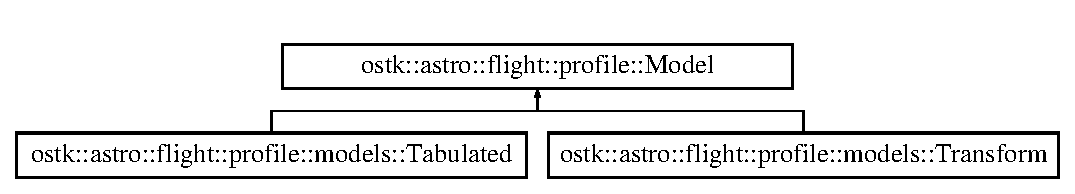
\includegraphics[height=2.000000cm]{classostk_1_1astro_1_1flight_1_1profile_1_1_model}
\end{center}
\end{figure}
\doxysubsection*{Public Member Functions}
\begin{DoxyCompactItemize}
\item 
\mbox{\hyperlink{classostk_1_1astro_1_1flight_1_1profile_1_1_model_a6301933ec5ccdd9dab16fa8ecbf73869}{Model}} ()
\item 
virtual \mbox{\hyperlink{classostk_1_1astro_1_1flight_1_1profile_1_1_model_a4870ff5251fa9f4f27f961700ce49863}{$\sim$\+Model}} ()=0
\item 
virtual \mbox{\hyperlink{classostk_1_1astro_1_1flight_1_1profile_1_1_model}{Model}} $\ast$ \mbox{\hyperlink{classostk_1_1astro_1_1flight_1_1profile_1_1_model_aabf68c114849fa16a570b694579da40f}{clone}} () const =0
\item 
virtual bool \mbox{\hyperlink{classostk_1_1astro_1_1flight_1_1profile_1_1_model_a87f7ca747d79619e4b4bc04aa6a9252a}{operator==}} (const \mbox{\hyperlink{classostk_1_1astro_1_1flight_1_1profile_1_1_model}{Model}} \&a\+Model) const =0
\item 
virtual bool \mbox{\hyperlink{classostk_1_1astro_1_1flight_1_1profile_1_1_model_a66eab26e18de60c179529ba5924b168f}{operator!=}} (const \mbox{\hyperlink{classostk_1_1astro_1_1flight_1_1profile_1_1_model}{Model}} \&a\+Model) const
\item 
virtual bool \mbox{\hyperlink{classostk_1_1astro_1_1flight_1_1profile_1_1_model_a0af64ad25ed8d8b2510a70bfe5bcb971}{is\+Defined}} () const =0
\item 
{\footnotesize template$<$class Type $>$ }\\bool \mbox{\hyperlink{classostk_1_1astro_1_1flight_1_1profile_1_1_model_a73363668308f0293014d6a77063cc809}{is}} () const
\begin{DoxyCompactList}\small\item\em Returns true if model can be converted to type. \end{DoxyCompactList}\item 
{\footnotesize template$<$class Type $>$ }\\const Type \& \mbox{\hyperlink{classostk_1_1astro_1_1flight_1_1profile_1_1_model_a7842761a8f6c0895c0b6048e9d3a5b7f}{as}} () const
\begin{DoxyCompactList}\small\item\em \mbox{\hyperlink{classostk_1_1astro_1_1_access}{Access}} model as its underlying type. \end{DoxyCompactList}\item 
virtual \mbox{\hyperlink{classostk_1_1astro_1_1flight_1_1profile_1_1_state}{State}} \mbox{\hyperlink{classostk_1_1astro_1_1flight_1_1profile_1_1_model_a1b205fa29b50fcfc06c99234a8579eb8}{calculate\+State\+At}} (const Instant \&an\+Instant) const =0
\item 
virtual Array$<$ \mbox{\hyperlink{classostk_1_1astro_1_1flight_1_1profile_1_1_state}{State}} $>$ \mbox{\hyperlink{classostk_1_1astro_1_1flight_1_1profile_1_1_model_ab81349e148cc39ad5662f7181f146493}{calculate\+States\+At}} (const Array$<$ Instant $>$ \&an\+Instant\+Array) const
\item 
virtual Axes \mbox{\hyperlink{classostk_1_1astro_1_1flight_1_1profile_1_1_model_ab18bd79e421c36df4ab716649ce549cd}{get\+Axes\+At}} (const Instant \&an\+Instant) const =0
\item 
virtual Shared$<$ const Frame $>$ \mbox{\hyperlink{classostk_1_1astro_1_1flight_1_1profile_1_1_model_a04ded49c09d9a44820251c48f47d0ffa}{get\+Body\+Frame}} (const String \&a\+Frame\+Name) const =0
\item 
virtual void \mbox{\hyperlink{classostk_1_1astro_1_1flight_1_1profile_1_1_model_ad9bb86b1869150e2bd970e9fa59ce36e}{print}} (std\+::ostream \&an\+Output\+Stream, bool display\+Decorator=true) const =0
\end{DoxyCompactItemize}
\doxysubsection*{Friends}
\begin{DoxyCompactItemize}
\item 
std\+::ostream \& \mbox{\hyperlink{classostk_1_1astro_1_1flight_1_1profile_1_1_model_a68240493d08f91f6613186eb52823e85}{operator$<$$<$}} (std\+::ostream \&an\+Output\+Stream, const \mbox{\hyperlink{classostk_1_1astro_1_1flight_1_1profile_1_1_model}{Model}} \&a\+Model)
\end{DoxyCompactItemize}


\doxysubsection{Detailed Description}
\mbox{\hyperlink{classostk_1_1astro_1_1flight_1_1_profile}{Profile}} model (abstract) 

\doxysubsection{Constructor \& Destructor Documentation}
\mbox{\Hypertarget{classostk_1_1astro_1_1flight_1_1profile_1_1_model_a6301933ec5ccdd9dab16fa8ecbf73869}\label{classostk_1_1astro_1_1flight_1_1profile_1_1_model_a6301933ec5ccdd9dab16fa8ecbf73869}} 
\index{ostk::astro::flight::profile::Model@{ostk::astro::flight::profile::Model}!Model@{Model}}
\index{Model@{Model}!ostk::astro::flight::profile::Model@{ostk::astro::flight::profile::Model}}
\doxysubsubsection{\texorpdfstring{Model()}{Model()}}
{\footnotesize\ttfamily ostk\+::astro\+::flight\+::profile\+::\+Model\+::\+Model (\begin{DoxyParamCaption}{ }\end{DoxyParamCaption})}

\mbox{\Hypertarget{classostk_1_1astro_1_1flight_1_1profile_1_1_model_a4870ff5251fa9f4f27f961700ce49863}\label{classostk_1_1astro_1_1flight_1_1profile_1_1_model_a4870ff5251fa9f4f27f961700ce49863}} 
\index{ostk::astro::flight::profile::Model@{ostk::astro::flight::profile::Model}!````~Model@{$\sim$Model}}
\index{````~Model@{$\sim$Model}!ostk::astro::flight::profile::Model@{ostk::astro::flight::profile::Model}}
\doxysubsubsection{\texorpdfstring{$\sim$Model()}{~Model()}}
{\footnotesize\ttfamily ostk\+::astro\+::flight\+::profile\+::\+Model\+::$\sim$\+Model (\begin{DoxyParamCaption}{ }\end{DoxyParamCaption})\hspace{0.3cm}{\ttfamily [pure virtual]}}



\doxysubsection{Member Function Documentation}
\mbox{\Hypertarget{classostk_1_1astro_1_1flight_1_1profile_1_1_model_a7842761a8f6c0895c0b6048e9d3a5b7f}\label{classostk_1_1astro_1_1flight_1_1profile_1_1_model_a7842761a8f6c0895c0b6048e9d3a5b7f}} 
\index{ostk::astro::flight::profile::Model@{ostk::astro::flight::profile::Model}!as@{as}}
\index{as@{as}!ostk::astro::flight::profile::Model@{ostk::astro::flight::profile::Model}}
\doxysubsubsection{\texorpdfstring{as()}{as()}}
{\footnotesize\ttfamily template$<$class Type $>$ \\
const Type\& ostk\+::astro\+::flight\+::profile\+::\+Model\+::as (\begin{DoxyParamCaption}{ }\end{DoxyParamCaption}) const\hspace{0.3cm}{\ttfamily [inline]}}



\mbox{\hyperlink{classostk_1_1astro_1_1_access}{Access}} model as its underlying type. 

\begin{DoxyReturn}{Returns}
Reference to underlying type 
\end{DoxyReturn}
\mbox{\Hypertarget{classostk_1_1astro_1_1flight_1_1profile_1_1_model_a1b205fa29b50fcfc06c99234a8579eb8}\label{classostk_1_1astro_1_1flight_1_1profile_1_1_model_a1b205fa29b50fcfc06c99234a8579eb8}} 
\index{ostk::astro::flight::profile::Model@{ostk::astro::flight::profile::Model}!calculateStateAt@{calculateStateAt}}
\index{calculateStateAt@{calculateStateAt}!ostk::astro::flight::profile::Model@{ostk::astro::flight::profile::Model}}
\doxysubsubsection{\texorpdfstring{calculateStateAt()}{calculateStateAt()}}
{\footnotesize\ttfamily virtual \mbox{\hyperlink{classostk_1_1astro_1_1flight_1_1profile_1_1_state}{State}} ostk\+::astro\+::flight\+::profile\+::\+Model\+::calculate\+State\+At (\begin{DoxyParamCaption}\item[{const Instant \&}]{an\+Instant }\end{DoxyParamCaption}) const\hspace{0.3cm}{\ttfamily [pure virtual]}}



Implemented in \mbox{\hyperlink{classostk_1_1astro_1_1flight_1_1profile_1_1models_1_1_tabulated_af27ea0e7006d0de18e897a9a5c7a0fb2}{ostk\+::astro\+::flight\+::profile\+::models\+::\+Tabulated}}, and \mbox{\hyperlink{classostk_1_1astro_1_1flight_1_1profile_1_1models_1_1_transform_a6288febae942c92508173db08b4554b0}{ostk\+::astro\+::flight\+::profile\+::models\+::\+Transform}}.

\mbox{\Hypertarget{classostk_1_1astro_1_1flight_1_1profile_1_1_model_ab81349e148cc39ad5662f7181f146493}\label{classostk_1_1astro_1_1flight_1_1profile_1_1_model_ab81349e148cc39ad5662f7181f146493}} 
\index{ostk::astro::flight::profile::Model@{ostk::astro::flight::profile::Model}!calculateStatesAt@{calculateStatesAt}}
\index{calculateStatesAt@{calculateStatesAt}!ostk::astro::flight::profile::Model@{ostk::astro::flight::profile::Model}}
\doxysubsubsection{\texorpdfstring{calculateStatesAt()}{calculateStatesAt()}}
{\footnotesize\ttfamily Array$<$ \mbox{\hyperlink{classostk_1_1astro_1_1flight_1_1profile_1_1_state}{State}} $>$ ostk\+::astro\+::flight\+::profile\+::\+Model\+::calculate\+States\+At (\begin{DoxyParamCaption}\item[{const Array$<$ Instant $>$ \&}]{an\+Instant\+Array }\end{DoxyParamCaption}) const\hspace{0.3cm}{\ttfamily [virtual]}}

\mbox{\Hypertarget{classostk_1_1astro_1_1flight_1_1profile_1_1_model_aabf68c114849fa16a570b694579da40f}\label{classostk_1_1astro_1_1flight_1_1profile_1_1_model_aabf68c114849fa16a570b694579da40f}} 
\index{ostk::astro::flight::profile::Model@{ostk::astro::flight::profile::Model}!clone@{clone}}
\index{clone@{clone}!ostk::astro::flight::profile::Model@{ostk::astro::flight::profile::Model}}
\doxysubsubsection{\texorpdfstring{clone()}{clone()}}
{\footnotesize\ttfamily virtual \mbox{\hyperlink{classostk_1_1astro_1_1flight_1_1profile_1_1_model}{Model}}$\ast$ ostk\+::astro\+::flight\+::profile\+::\+Model\+::clone (\begin{DoxyParamCaption}{ }\end{DoxyParamCaption}) const\hspace{0.3cm}{\ttfamily [pure virtual]}}



Implemented in \mbox{\hyperlink{classostk_1_1astro_1_1flight_1_1profile_1_1models_1_1_tabulated_a1c9f4f5711ac2ae0cc545d89b0ee4d53}{ostk\+::astro\+::flight\+::profile\+::models\+::\+Tabulated}}, and \mbox{\hyperlink{classostk_1_1astro_1_1flight_1_1profile_1_1models_1_1_transform_aafd4791dacf320ddedddefbc8d0f2e0e}{ostk\+::astro\+::flight\+::profile\+::models\+::\+Transform}}.

\mbox{\Hypertarget{classostk_1_1astro_1_1flight_1_1profile_1_1_model_ab18bd79e421c36df4ab716649ce549cd}\label{classostk_1_1astro_1_1flight_1_1profile_1_1_model_ab18bd79e421c36df4ab716649ce549cd}} 
\index{ostk::astro::flight::profile::Model@{ostk::astro::flight::profile::Model}!getAxesAt@{getAxesAt}}
\index{getAxesAt@{getAxesAt}!ostk::astro::flight::profile::Model@{ostk::astro::flight::profile::Model}}
\doxysubsubsection{\texorpdfstring{getAxesAt()}{getAxesAt()}}
{\footnotesize\ttfamily virtual Axes ostk\+::astro\+::flight\+::profile\+::\+Model\+::get\+Axes\+At (\begin{DoxyParamCaption}\item[{const Instant \&}]{an\+Instant }\end{DoxyParamCaption}) const\hspace{0.3cm}{\ttfamily [pure virtual]}}



Implemented in \mbox{\hyperlink{classostk_1_1astro_1_1flight_1_1profile_1_1models_1_1_tabulated_ac85970f439c8db0684c9349601c226d2}{ostk\+::astro\+::flight\+::profile\+::models\+::\+Tabulated}}, and \mbox{\hyperlink{classostk_1_1astro_1_1flight_1_1profile_1_1models_1_1_transform_a7eb8b58fd5f72e8ee9aa3b94cd0ffaaa}{ostk\+::astro\+::flight\+::profile\+::models\+::\+Transform}}.

\mbox{\Hypertarget{classostk_1_1astro_1_1flight_1_1profile_1_1_model_a04ded49c09d9a44820251c48f47d0ffa}\label{classostk_1_1astro_1_1flight_1_1profile_1_1_model_a04ded49c09d9a44820251c48f47d0ffa}} 
\index{ostk::astro::flight::profile::Model@{ostk::astro::flight::profile::Model}!getBodyFrame@{getBodyFrame}}
\index{getBodyFrame@{getBodyFrame}!ostk::astro::flight::profile::Model@{ostk::astro::flight::profile::Model}}
\doxysubsubsection{\texorpdfstring{getBodyFrame()}{getBodyFrame()}}
{\footnotesize\ttfamily virtual Shared$<$const Frame$>$ ostk\+::astro\+::flight\+::profile\+::\+Model\+::get\+Body\+Frame (\begin{DoxyParamCaption}\item[{const String \&}]{a\+Frame\+Name }\end{DoxyParamCaption}) const\hspace{0.3cm}{\ttfamily [pure virtual]}}



Implemented in \mbox{\hyperlink{classostk_1_1astro_1_1flight_1_1profile_1_1models_1_1_tabulated_a1be1d71748e4e0b59bd3dd2334b759fe}{ostk\+::astro\+::flight\+::profile\+::models\+::\+Tabulated}}, and \mbox{\hyperlink{classostk_1_1astro_1_1flight_1_1profile_1_1models_1_1_transform_a7fa6ee57c59b5bff2c60001c11cac04c}{ostk\+::astro\+::flight\+::profile\+::models\+::\+Transform}}.

\mbox{\Hypertarget{classostk_1_1astro_1_1flight_1_1profile_1_1_model_a73363668308f0293014d6a77063cc809}\label{classostk_1_1astro_1_1flight_1_1profile_1_1_model_a73363668308f0293014d6a77063cc809}} 
\index{ostk::astro::flight::profile::Model@{ostk::astro::flight::profile::Model}!is@{is}}
\index{is@{is}!ostk::astro::flight::profile::Model@{ostk::astro::flight::profile::Model}}
\doxysubsubsection{\texorpdfstring{is()}{is()}}
{\footnotesize\ttfamily template$<$class Type $>$ \\
bool ostk\+::astro\+::flight\+::profile\+::\+Model\+::is (\begin{DoxyParamCaption}{ }\end{DoxyParamCaption}) const\hspace{0.3cm}{\ttfamily [inline]}}



Returns true if model can be converted to type. 

\begin{DoxyReturn}{Returns}
True if model can be converted to type 
\end{DoxyReturn}
\mbox{\Hypertarget{classostk_1_1astro_1_1flight_1_1profile_1_1_model_a0af64ad25ed8d8b2510a70bfe5bcb971}\label{classostk_1_1astro_1_1flight_1_1profile_1_1_model_a0af64ad25ed8d8b2510a70bfe5bcb971}} 
\index{ostk::astro::flight::profile::Model@{ostk::astro::flight::profile::Model}!isDefined@{isDefined}}
\index{isDefined@{isDefined}!ostk::astro::flight::profile::Model@{ostk::astro::flight::profile::Model}}
\doxysubsubsection{\texorpdfstring{isDefined()}{isDefined()}}
{\footnotesize\ttfamily virtual bool ostk\+::astro\+::flight\+::profile\+::\+Model\+::is\+Defined (\begin{DoxyParamCaption}{ }\end{DoxyParamCaption}) const\hspace{0.3cm}{\ttfamily [pure virtual]}}



Implemented in \mbox{\hyperlink{classostk_1_1astro_1_1flight_1_1profile_1_1models_1_1_tabulated_ad830d557475ca2ba83d43659e348b1d6}{ostk\+::astro\+::flight\+::profile\+::models\+::\+Tabulated}}, and \mbox{\hyperlink{classostk_1_1astro_1_1flight_1_1profile_1_1models_1_1_transform_a2d0f1f3cc3f340c5617125bea08a9930}{ostk\+::astro\+::flight\+::profile\+::models\+::\+Transform}}.

\mbox{\Hypertarget{classostk_1_1astro_1_1flight_1_1profile_1_1_model_a66eab26e18de60c179529ba5924b168f}\label{classostk_1_1astro_1_1flight_1_1profile_1_1_model_a66eab26e18de60c179529ba5924b168f}} 
\index{ostk::astro::flight::profile::Model@{ostk::astro::flight::profile::Model}!operator"!=@{operator"!=}}
\index{operator"!=@{operator"!=}!ostk::astro::flight::profile::Model@{ostk::astro::flight::profile::Model}}
\doxysubsubsection{\texorpdfstring{operator"!=()}{operator!=()}}
{\footnotesize\ttfamily bool ostk\+::astro\+::flight\+::profile\+::\+Model\+::operator!= (\begin{DoxyParamCaption}\item[{const \mbox{\hyperlink{classostk_1_1astro_1_1flight_1_1profile_1_1_model}{Model}} \&}]{a\+Model }\end{DoxyParamCaption}) const\hspace{0.3cm}{\ttfamily [virtual]}}



Reimplemented in \mbox{\hyperlink{classostk_1_1astro_1_1flight_1_1profile_1_1models_1_1_tabulated_a7d1f3f2024628e03eee408eaa1cd1a9b}{ostk\+::astro\+::flight\+::profile\+::models\+::\+Tabulated}}.

\mbox{\Hypertarget{classostk_1_1astro_1_1flight_1_1profile_1_1_model_a87f7ca747d79619e4b4bc04aa6a9252a}\label{classostk_1_1astro_1_1flight_1_1profile_1_1_model_a87f7ca747d79619e4b4bc04aa6a9252a}} 
\index{ostk::astro::flight::profile::Model@{ostk::astro::flight::profile::Model}!operator==@{operator==}}
\index{operator==@{operator==}!ostk::astro::flight::profile::Model@{ostk::astro::flight::profile::Model}}
\doxysubsubsection{\texorpdfstring{operator==()}{operator==()}}
{\footnotesize\ttfamily virtual bool ostk\+::astro\+::flight\+::profile\+::\+Model\+::operator== (\begin{DoxyParamCaption}\item[{const \mbox{\hyperlink{classostk_1_1astro_1_1flight_1_1profile_1_1_model}{Model}} \&}]{a\+Model }\end{DoxyParamCaption}) const\hspace{0.3cm}{\ttfamily [pure virtual]}}



Implemented in \mbox{\hyperlink{classostk_1_1astro_1_1flight_1_1profile_1_1models_1_1_transform_ad49694ca5cfb4fabf17ac063d9953fb0}{ostk\+::astro\+::flight\+::profile\+::models\+::\+Transform}}, and \mbox{\hyperlink{classostk_1_1astro_1_1flight_1_1profile_1_1models_1_1_tabulated_a5fd04ff2470cfe517bcb94e70fdb80fd}{ostk\+::astro\+::flight\+::profile\+::models\+::\+Tabulated}}.

\mbox{\Hypertarget{classostk_1_1astro_1_1flight_1_1profile_1_1_model_ad9bb86b1869150e2bd970e9fa59ce36e}\label{classostk_1_1astro_1_1flight_1_1profile_1_1_model_ad9bb86b1869150e2bd970e9fa59ce36e}} 
\index{ostk::astro::flight::profile::Model@{ostk::astro::flight::profile::Model}!print@{print}}
\index{print@{print}!ostk::astro::flight::profile::Model@{ostk::astro::flight::profile::Model}}
\doxysubsubsection{\texorpdfstring{print()}{print()}}
{\footnotesize\ttfamily virtual void ostk\+::astro\+::flight\+::profile\+::\+Model\+::print (\begin{DoxyParamCaption}\item[{std\+::ostream \&}]{an\+Output\+Stream,  }\item[{bool}]{display\+Decorator = {\ttfamily true} }\end{DoxyParamCaption}) const\hspace{0.3cm}{\ttfamily [pure virtual]}}



Implemented in \mbox{\hyperlink{classostk_1_1astro_1_1flight_1_1profile_1_1models_1_1_tabulated_a0e3d34c39a644279a9b958c3fd9bf730}{ostk\+::astro\+::flight\+::profile\+::models\+::\+Tabulated}}, and \mbox{\hyperlink{classostk_1_1astro_1_1flight_1_1profile_1_1models_1_1_transform_aef9a20156493d68570a989d87ac2f9f6}{ostk\+::astro\+::flight\+::profile\+::models\+::\+Transform}}.



\doxysubsection{Friends And Related Function Documentation}
\mbox{\Hypertarget{classostk_1_1astro_1_1flight_1_1profile_1_1_model_a68240493d08f91f6613186eb52823e85}\label{classostk_1_1astro_1_1flight_1_1profile_1_1_model_a68240493d08f91f6613186eb52823e85}} 
\index{ostk::astro::flight::profile::Model@{ostk::astro::flight::profile::Model}!operator$<$$<$@{operator$<$$<$}}
\index{operator$<$$<$@{operator$<$$<$}!ostk::astro::flight::profile::Model@{ostk::astro::flight::profile::Model}}
\doxysubsubsection{\texorpdfstring{operator$<$$<$}{operator<<}}
{\footnotesize\ttfamily std\+::ostream\& operator$<$$<$ (\begin{DoxyParamCaption}\item[{std\+::ostream \&}]{an\+Output\+Stream,  }\item[{const \mbox{\hyperlink{classostk_1_1astro_1_1flight_1_1profile_1_1_model}{Model}} \&}]{a\+Model }\end{DoxyParamCaption})\hspace{0.3cm}{\ttfamily [friend]}}



The documentation for this class was generated from the following files\+:\begin{DoxyCompactItemize}
\item 
include/\+Open\+Space\+Toolkit/\+Astrodynamics/\+Flight/\+Profile/\mbox{\hyperlink{_flight_2_profile_2_model_8hpp}{Model.\+hpp}}\item 
src/\+Open\+Space\+Toolkit/\+Astrodynamics/\+Flight/\+Profile/\mbox{\hyperlink{_flight_2_profile_2_model_8cpp}{Model.\+cpp}}\end{DoxyCompactItemize}

\hypertarget{classostk_1_1astro_1_1trajectory_1_1_model}{}\doxysection{ostk\+::astro\+::trajectory\+::Model Class Reference}
\label{classostk_1_1astro_1_1trajectory_1_1_model}\index{ostk::astro::trajectory::Model@{ostk::astro::trajectory::Model}}


\mbox{\hyperlink{classostk_1_1astro_1_1_trajectory}{Trajectory}} model (abstract)  




{\ttfamily \#include $<$Model.\+hpp$>$}

Inheritance diagram for ostk\+::astro\+::trajectory\+::Model\+:\begin{figure}[H]
\begin{center}
\leavevmode
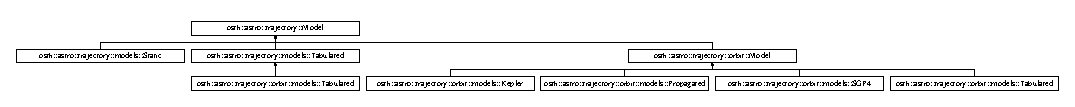
\includegraphics[height=0.989399cm]{classostk_1_1astro_1_1trajectory_1_1_model}
\end{center}
\end{figure}
\doxysubsection*{Public Member Functions}
\begin{DoxyCompactItemize}
\item 
\mbox{\hyperlink{classostk_1_1astro_1_1trajectory_1_1_model_aed4bcf4fbd44f69e97d8ff98112aa0f5}{Model}} ()
\item 
virtual \mbox{\hyperlink{classostk_1_1astro_1_1trajectory_1_1_model_a23acd7acccf729d8343180b83fe2f9f9}{$\sim$\+Model}} ()=0
\item 
virtual \mbox{\hyperlink{classostk_1_1astro_1_1trajectory_1_1_model}{Model}} $\ast$ \mbox{\hyperlink{classostk_1_1astro_1_1trajectory_1_1_model_ad9f1467f711b07796ddc1437fb9ad9df}{clone}} () const =0
\item 
virtual bool \mbox{\hyperlink{classostk_1_1astro_1_1trajectory_1_1_model_a874f79846e845859c070ce1b9874fc9c}{operator==}} (const \mbox{\hyperlink{classostk_1_1astro_1_1trajectory_1_1_model}{Model}} \&a\+Model) const =0
\item 
virtual bool \mbox{\hyperlink{classostk_1_1astro_1_1trajectory_1_1_model_a2dd77b9f6939d738f3a489f26c955340}{operator!=}} (const \mbox{\hyperlink{classostk_1_1astro_1_1trajectory_1_1_model}{Model}} \&a\+Model) const =0
\item 
virtual bool \mbox{\hyperlink{classostk_1_1astro_1_1trajectory_1_1_model_a0d5cf6f754905f06c0ec1e39618c20a1}{is\+Defined}} () const =0
\item 
{\footnotesize template$<$class Type $>$ }\\bool \mbox{\hyperlink{classostk_1_1astro_1_1trajectory_1_1_model_aedde1c01efbf407cca64b3f18b1a60f2}{is}} () const
\begin{DoxyCompactList}\small\item\em Returns true if model can be converted to type. \end{DoxyCompactList}\item 
{\footnotesize template$<$class Type $>$ }\\const Type \& \mbox{\hyperlink{classostk_1_1astro_1_1trajectory_1_1_model_a53365ee40062f5571b664998a56701e3}{as}} () const
\begin{DoxyCompactList}\small\item\em \mbox{\hyperlink{classostk_1_1astro_1_1_access}{Access}} model as its underlying type. \end{DoxyCompactList}\item 
virtual \mbox{\hyperlink{classostk_1_1astro_1_1trajectory_1_1_state}{State}} \mbox{\hyperlink{classostk_1_1astro_1_1trajectory_1_1_model_ad25eeaded2946bf73d44161b5f4e9a0e}{calculate\+State\+At}} (const Instant \&an\+Instant) const =0
\item 
virtual Array$<$ \mbox{\hyperlink{classostk_1_1astro_1_1trajectory_1_1_state}{State}} $>$ \mbox{\hyperlink{classostk_1_1astro_1_1trajectory_1_1_model_a3c3e4913aed2272174c0e6cd0d1a6415}{calculate\+States\+At}} (const Array$<$ Instant $>$ \&an\+Instant\+Array) const
\item 
virtual void \mbox{\hyperlink{classostk_1_1astro_1_1trajectory_1_1_model_a4b2098483430a820481ed50b81656e31}{print}} (std\+::ostream \&an\+Output\+Stream, bool display\+Decorator=true) const =0
\end{DoxyCompactItemize}
\doxysubsection*{Friends}
\begin{DoxyCompactItemize}
\item 
std\+::ostream \& \mbox{\hyperlink{classostk_1_1astro_1_1trajectory_1_1_model_a68240493d08f91f6613186eb52823e85}{operator$<$$<$}} (std\+::ostream \&an\+Output\+Stream, const \mbox{\hyperlink{classostk_1_1astro_1_1trajectory_1_1_model}{Model}} \&a\+Model)
\end{DoxyCompactItemize}


\doxysubsection{Detailed Description}
\mbox{\hyperlink{classostk_1_1astro_1_1_trajectory}{Trajectory}} model (abstract) 

\doxysubsection{Constructor \& Destructor Documentation}
\mbox{\Hypertarget{classostk_1_1astro_1_1trajectory_1_1_model_aed4bcf4fbd44f69e97d8ff98112aa0f5}\label{classostk_1_1astro_1_1trajectory_1_1_model_aed4bcf4fbd44f69e97d8ff98112aa0f5}} 
\index{ostk::astro::trajectory::Model@{ostk::astro::trajectory::Model}!Model@{Model}}
\index{Model@{Model}!ostk::astro::trajectory::Model@{ostk::astro::trajectory::Model}}
\doxysubsubsection{\texorpdfstring{Model()}{Model()}}
{\footnotesize\ttfamily ostk\+::astro\+::trajectory\+::\+Model\+::\+Model (\begin{DoxyParamCaption}{ }\end{DoxyParamCaption})}

\mbox{\Hypertarget{classostk_1_1astro_1_1trajectory_1_1_model_a23acd7acccf729d8343180b83fe2f9f9}\label{classostk_1_1astro_1_1trajectory_1_1_model_a23acd7acccf729d8343180b83fe2f9f9}} 
\index{ostk::astro::trajectory::Model@{ostk::astro::trajectory::Model}!````~Model@{$\sim$Model}}
\index{````~Model@{$\sim$Model}!ostk::astro::trajectory::Model@{ostk::astro::trajectory::Model}}
\doxysubsubsection{\texorpdfstring{$\sim$Model()}{~Model()}}
{\footnotesize\ttfamily ostk\+::astro\+::trajectory\+::\+Model\+::$\sim$\+Model (\begin{DoxyParamCaption}{ }\end{DoxyParamCaption})\hspace{0.3cm}{\ttfamily [pure virtual]}}



Implemented in \mbox{\hyperlink{classostk_1_1astro_1_1trajectory_1_1orbit_1_1_model_a7593c3eccd08104b00dd4d7c9c6a4d99}{ostk\+::astro\+::trajectory\+::orbit\+::\+Model}}.



\doxysubsection{Member Function Documentation}
\mbox{\Hypertarget{classostk_1_1astro_1_1trajectory_1_1_model_a53365ee40062f5571b664998a56701e3}\label{classostk_1_1astro_1_1trajectory_1_1_model_a53365ee40062f5571b664998a56701e3}} 
\index{ostk::astro::trajectory::Model@{ostk::astro::trajectory::Model}!as@{as}}
\index{as@{as}!ostk::astro::trajectory::Model@{ostk::astro::trajectory::Model}}
\doxysubsubsection{\texorpdfstring{as()}{as()}}
{\footnotesize\ttfamily template$<$class Type $>$ \\
const Type\& ostk\+::astro\+::trajectory\+::\+Model\+::as (\begin{DoxyParamCaption}{ }\end{DoxyParamCaption}) const\hspace{0.3cm}{\ttfamily [inline]}}



\mbox{\hyperlink{classostk_1_1astro_1_1_access}{Access}} model as its underlying type. 

\begin{DoxyReturn}{Returns}
Reference to underlying type 
\end{DoxyReturn}
\mbox{\Hypertarget{classostk_1_1astro_1_1trajectory_1_1_model_ad25eeaded2946bf73d44161b5f4e9a0e}\label{classostk_1_1astro_1_1trajectory_1_1_model_ad25eeaded2946bf73d44161b5f4e9a0e}} 
\index{ostk::astro::trajectory::Model@{ostk::astro::trajectory::Model}!calculateStateAt@{calculateStateAt}}
\index{calculateStateAt@{calculateStateAt}!ostk::astro::trajectory::Model@{ostk::astro::trajectory::Model}}
\doxysubsubsection{\texorpdfstring{calculateStateAt()}{calculateStateAt()}}
{\footnotesize\ttfamily virtual \mbox{\hyperlink{classostk_1_1astro_1_1trajectory_1_1_state}{State}} ostk\+::astro\+::trajectory\+::\+Model\+::calculate\+State\+At (\begin{DoxyParamCaption}\item[{const Instant \&}]{an\+Instant }\end{DoxyParamCaption}) const\hspace{0.3cm}{\ttfamily [pure virtual]}}



Implemented in \mbox{\hyperlink{classostk_1_1astro_1_1trajectory_1_1orbit_1_1models_1_1_propagated_a2efc3c1af735dcf2ec622d056fa0a13f}{ostk\+::astro\+::trajectory\+::orbit\+::models\+::\+Propagated}}, \mbox{\hyperlink{classostk_1_1astro_1_1trajectory_1_1orbit_1_1models_1_1_kepler_a4de0c3d7a2b37c1c2ab4d6e207339809}{ostk\+::astro\+::trajectory\+::orbit\+::models\+::\+Kepler}}, \mbox{\hyperlink{classostk_1_1astro_1_1trajectory_1_1models_1_1_tabulated_af2ebaa6456986636aa58c2f8666ed0b9}{ostk\+::astro\+::trajectory\+::models\+::\+Tabulated}}, \mbox{\hyperlink{classostk_1_1astro_1_1trajectory_1_1orbit_1_1models_1_1_s_g_p4_ad88439d9c46a75d3da8c20d2872271e3}{ostk\+::astro\+::trajectory\+::orbit\+::models\+::\+S\+G\+P4}}, \mbox{\hyperlink{classostk_1_1astro_1_1trajectory_1_1orbit_1_1models_1_1_tabulated_ad7935cafe71b572b97b9df93e469d2f8}{ostk\+::astro\+::trajectory\+::orbit\+::models\+::\+Tabulated}}, \mbox{\hyperlink{classostk_1_1astro_1_1trajectory_1_1models_1_1_static_a4297a74c953a105dc887a31227fbe1ff}{ostk\+::astro\+::trajectory\+::models\+::\+Static}}, and \mbox{\hyperlink{classostk_1_1astro_1_1trajectory_1_1orbit_1_1_model_a34a0d8979ec1f7ade3e434fc0dad3711}{ostk\+::astro\+::trajectory\+::orbit\+::\+Model}}.

\mbox{\Hypertarget{classostk_1_1astro_1_1trajectory_1_1_model_a3c3e4913aed2272174c0e6cd0d1a6415}\label{classostk_1_1astro_1_1trajectory_1_1_model_a3c3e4913aed2272174c0e6cd0d1a6415}} 
\index{ostk::astro::trajectory::Model@{ostk::astro::trajectory::Model}!calculateStatesAt@{calculateStatesAt}}
\index{calculateStatesAt@{calculateStatesAt}!ostk::astro::trajectory::Model@{ostk::astro::trajectory::Model}}
\doxysubsubsection{\texorpdfstring{calculateStatesAt()}{calculateStatesAt()}}
{\footnotesize\ttfamily Array$<$ \mbox{\hyperlink{classostk_1_1astro_1_1trajectory_1_1_state}{State}} $>$ ostk\+::astro\+::trajectory\+::\+Model\+::calculate\+States\+At (\begin{DoxyParamCaption}\item[{const Array$<$ Instant $>$ \&}]{an\+Instant\+Array }\end{DoxyParamCaption}) const\hspace{0.3cm}{\ttfamily [virtual]}}



Reimplemented in \mbox{\hyperlink{classostk_1_1astro_1_1trajectory_1_1orbit_1_1models_1_1_propagated_a9a4097432d2c863aedead23d2d67a7a7}{ostk\+::astro\+::trajectory\+::orbit\+::models\+::\+Propagated}}, and \mbox{\hyperlink{classostk_1_1astro_1_1trajectory_1_1models_1_1_tabulated_a32239d967738b2625504bc5efe8737eb}{ostk\+::astro\+::trajectory\+::models\+::\+Tabulated}}.

\mbox{\Hypertarget{classostk_1_1astro_1_1trajectory_1_1_model_ad9f1467f711b07796ddc1437fb9ad9df}\label{classostk_1_1astro_1_1trajectory_1_1_model_ad9f1467f711b07796ddc1437fb9ad9df}} 
\index{ostk::astro::trajectory::Model@{ostk::astro::trajectory::Model}!clone@{clone}}
\index{clone@{clone}!ostk::astro::trajectory::Model@{ostk::astro::trajectory::Model}}
\doxysubsubsection{\texorpdfstring{clone()}{clone()}}
{\footnotesize\ttfamily virtual \mbox{\hyperlink{classostk_1_1astro_1_1trajectory_1_1_model}{Model}}$\ast$ ostk\+::astro\+::trajectory\+::\+Model\+::clone (\begin{DoxyParamCaption}{ }\end{DoxyParamCaption}) const\hspace{0.3cm}{\ttfamily [pure virtual]}}



Implemented in \mbox{\hyperlink{classostk_1_1astro_1_1trajectory_1_1models_1_1_tabulated_a553d2c4027ce269c1c2b3f4e9c65e14d}{ostk\+::astro\+::trajectory\+::models\+::\+Tabulated}}, \mbox{\hyperlink{classostk_1_1astro_1_1trajectory_1_1orbit_1_1models_1_1_kepler_afb76b3571c73fb5c87129033f7d66520}{ostk\+::astro\+::trajectory\+::orbit\+::models\+::\+Kepler}}, \mbox{\hyperlink{classostk_1_1astro_1_1trajectory_1_1orbit_1_1models_1_1_propagated_a283639d985495c05adb9e80edb91cd12}{ostk\+::astro\+::trajectory\+::orbit\+::models\+::\+Propagated}}, \mbox{\hyperlink{classostk_1_1astro_1_1trajectory_1_1orbit_1_1models_1_1_s_g_p4_afb9928e09d66c13a77eb1126da6139eb}{ostk\+::astro\+::trajectory\+::orbit\+::models\+::\+S\+G\+P4}}, \mbox{\hyperlink{classostk_1_1astro_1_1trajectory_1_1orbit_1_1models_1_1_tabulated_a53603727c33f9ff8db520831cf666142}{ostk\+::astro\+::trajectory\+::orbit\+::models\+::\+Tabulated}}, \mbox{\hyperlink{classostk_1_1astro_1_1trajectory_1_1models_1_1_static_abe3edbc72ae2f4fbd6c2593e2aa08755}{ostk\+::astro\+::trajectory\+::models\+::\+Static}}, and \mbox{\hyperlink{classostk_1_1astro_1_1trajectory_1_1orbit_1_1_model_a53dc07564e4c7c444da46360aa8ada15}{ostk\+::astro\+::trajectory\+::orbit\+::\+Model}}.

\mbox{\Hypertarget{classostk_1_1astro_1_1trajectory_1_1_model_aedde1c01efbf407cca64b3f18b1a60f2}\label{classostk_1_1astro_1_1trajectory_1_1_model_aedde1c01efbf407cca64b3f18b1a60f2}} 
\index{ostk::astro::trajectory::Model@{ostk::astro::trajectory::Model}!is@{is}}
\index{is@{is}!ostk::astro::trajectory::Model@{ostk::astro::trajectory::Model}}
\doxysubsubsection{\texorpdfstring{is()}{is()}}
{\footnotesize\ttfamily template$<$class Type $>$ \\
bool ostk\+::astro\+::trajectory\+::\+Model\+::is (\begin{DoxyParamCaption}{ }\end{DoxyParamCaption}) const\hspace{0.3cm}{\ttfamily [inline]}}



Returns true if model can be converted to type. 

\begin{DoxyReturn}{Returns}
True if model can be converted to type 
\end{DoxyReturn}
\mbox{\Hypertarget{classostk_1_1astro_1_1trajectory_1_1_model_a0d5cf6f754905f06c0ec1e39618c20a1}\label{classostk_1_1astro_1_1trajectory_1_1_model_a0d5cf6f754905f06c0ec1e39618c20a1}} 
\index{ostk::astro::trajectory::Model@{ostk::astro::trajectory::Model}!isDefined@{isDefined}}
\index{isDefined@{isDefined}!ostk::astro::trajectory::Model@{ostk::astro::trajectory::Model}}
\doxysubsubsection{\texorpdfstring{isDefined()}{isDefined()}}
{\footnotesize\ttfamily virtual bool ostk\+::astro\+::trajectory\+::\+Model\+::is\+Defined (\begin{DoxyParamCaption}{ }\end{DoxyParamCaption}) const\hspace{0.3cm}{\ttfamily [pure virtual]}}



Implemented in \mbox{\hyperlink{classostk_1_1astro_1_1trajectory_1_1orbit_1_1models_1_1_propagated_a530fd6bc017c74dedc43ced5fe843a03}{ostk\+::astro\+::trajectory\+::orbit\+::models\+::\+Propagated}}, \mbox{\hyperlink{classostk_1_1astro_1_1trajectory_1_1models_1_1_tabulated_a379da4c10a738c3f4578042c9bae0c91}{ostk\+::astro\+::trajectory\+::models\+::\+Tabulated}}, \mbox{\hyperlink{classostk_1_1astro_1_1trajectory_1_1orbit_1_1models_1_1_kepler_a4c74402d5483a51e5e0fe1920cd52ec4}{ostk\+::astro\+::trajectory\+::orbit\+::models\+::\+Kepler}}, \mbox{\hyperlink{classostk_1_1astro_1_1trajectory_1_1orbit_1_1models_1_1_s_g_p4_ab18e0666588bd517c190942b1a54ed18}{ostk\+::astro\+::trajectory\+::orbit\+::models\+::\+S\+G\+P4}}, \mbox{\hyperlink{classostk_1_1astro_1_1trajectory_1_1orbit_1_1models_1_1_tabulated_ad114ba4762b54211f74f0aa3ac5eedae}{ostk\+::astro\+::trajectory\+::orbit\+::models\+::\+Tabulated}}, \mbox{\hyperlink{classostk_1_1astro_1_1trajectory_1_1models_1_1_static_a5a80d75c9215af9b198c9f8653c5bc17}{ostk\+::astro\+::trajectory\+::models\+::\+Static}}, and \mbox{\hyperlink{classostk_1_1astro_1_1trajectory_1_1orbit_1_1_model_a13c5b5693dd86a072da0bd0e319bacc2}{ostk\+::astro\+::trajectory\+::orbit\+::\+Model}}.

\mbox{\Hypertarget{classostk_1_1astro_1_1trajectory_1_1_model_a2dd77b9f6939d738f3a489f26c955340}\label{classostk_1_1astro_1_1trajectory_1_1_model_a2dd77b9f6939d738f3a489f26c955340}} 
\index{ostk::astro::trajectory::Model@{ostk::astro::trajectory::Model}!operator"!=@{operator"!=}}
\index{operator"!=@{operator"!=}!ostk::astro::trajectory::Model@{ostk::astro::trajectory::Model}}
\doxysubsubsection{\texorpdfstring{operator"!=()}{operator!=()}}
{\footnotesize\ttfamily virtual bool ostk\+::astro\+::trajectory\+::\+Model\+::operator!= (\begin{DoxyParamCaption}\item[{const \mbox{\hyperlink{classostk_1_1astro_1_1trajectory_1_1_model}{Model}} \&}]{a\+Model }\end{DoxyParamCaption}) const\hspace{0.3cm}{\ttfamily [pure virtual]}}



Implemented in \mbox{\hyperlink{classostk_1_1astro_1_1trajectory_1_1orbit_1_1models_1_1_propagated_aeffaddcde5540fd1226add8466415d08}{ostk\+::astro\+::trajectory\+::orbit\+::models\+::\+Propagated}}, \mbox{\hyperlink{classostk_1_1astro_1_1trajectory_1_1orbit_1_1models_1_1_kepler_ab343575a423c5cecea4b21fa79c80726}{ostk\+::astro\+::trajectory\+::orbit\+::models\+::\+Kepler}}, \mbox{\hyperlink{classostk_1_1astro_1_1trajectory_1_1orbit_1_1models_1_1_s_g_p4_a87441104e4e1c63356abe0632b56edb6}{ostk\+::astro\+::trajectory\+::orbit\+::models\+::\+S\+G\+P4}}, \mbox{\hyperlink{classostk_1_1astro_1_1trajectory_1_1orbit_1_1models_1_1_tabulated_a17610dc24fefecd03ae595cc78ef3079}{ostk\+::astro\+::trajectory\+::orbit\+::models\+::\+Tabulated}}, \mbox{\hyperlink{classostk_1_1astro_1_1trajectory_1_1models_1_1_tabulated_a5e047165eb79ea50d257c2cb1bafc30d}{ostk\+::astro\+::trajectory\+::models\+::\+Tabulated}}, and \mbox{\hyperlink{classostk_1_1astro_1_1trajectory_1_1models_1_1_static_af85efc113db69c75c1afc7db0e81297b}{ostk\+::astro\+::trajectory\+::models\+::\+Static}}.

\mbox{\Hypertarget{classostk_1_1astro_1_1trajectory_1_1_model_a874f79846e845859c070ce1b9874fc9c}\label{classostk_1_1astro_1_1trajectory_1_1_model_a874f79846e845859c070ce1b9874fc9c}} 
\index{ostk::astro::trajectory::Model@{ostk::astro::trajectory::Model}!operator==@{operator==}}
\index{operator==@{operator==}!ostk::astro::trajectory::Model@{ostk::astro::trajectory::Model}}
\doxysubsubsection{\texorpdfstring{operator==()}{operator==()}}
{\footnotesize\ttfamily virtual bool ostk\+::astro\+::trajectory\+::\+Model\+::operator== (\begin{DoxyParamCaption}\item[{const \mbox{\hyperlink{classostk_1_1astro_1_1trajectory_1_1_model}{Model}} \&}]{a\+Model }\end{DoxyParamCaption}) const\hspace{0.3cm}{\ttfamily [pure virtual]}}



Implemented in \mbox{\hyperlink{classostk_1_1astro_1_1trajectory_1_1orbit_1_1models_1_1_propagated_a29b52ccf653fbd84699edab0f198f590}{ostk\+::astro\+::trajectory\+::orbit\+::models\+::\+Propagated}}, \mbox{\hyperlink{classostk_1_1astro_1_1trajectory_1_1orbit_1_1models_1_1_kepler_ad2a61eb0cbd9887fc2180dc0818c209e}{ostk\+::astro\+::trajectory\+::orbit\+::models\+::\+Kepler}}, \mbox{\hyperlink{classostk_1_1astro_1_1trajectory_1_1orbit_1_1models_1_1_s_g_p4_ad51d979b8b9b37251b6381cfe9df55ea}{ostk\+::astro\+::trajectory\+::orbit\+::models\+::\+S\+G\+P4}}, \mbox{\hyperlink{classostk_1_1astro_1_1trajectory_1_1orbit_1_1models_1_1_tabulated_abd72010cb413d8479c097376bfebaf56}{ostk\+::astro\+::trajectory\+::orbit\+::models\+::\+Tabulated}}, \mbox{\hyperlink{classostk_1_1astro_1_1trajectory_1_1models_1_1_tabulated_a9d206aee35ebabe4b36ddfc057142f16}{ostk\+::astro\+::trajectory\+::models\+::\+Tabulated}}, and \mbox{\hyperlink{classostk_1_1astro_1_1trajectory_1_1models_1_1_static_a0ef36b672baa80f522135d86f3b6bb9c}{ostk\+::astro\+::trajectory\+::models\+::\+Static}}.

\mbox{\Hypertarget{classostk_1_1astro_1_1trajectory_1_1_model_a4b2098483430a820481ed50b81656e31}\label{classostk_1_1astro_1_1trajectory_1_1_model_a4b2098483430a820481ed50b81656e31}} 
\index{ostk::astro::trajectory::Model@{ostk::astro::trajectory::Model}!print@{print}}
\index{print@{print}!ostk::astro::trajectory::Model@{ostk::astro::trajectory::Model}}
\doxysubsubsection{\texorpdfstring{print()}{print()}}
{\footnotesize\ttfamily virtual void ostk\+::astro\+::trajectory\+::\+Model\+::print (\begin{DoxyParamCaption}\item[{std\+::ostream \&}]{an\+Output\+Stream,  }\item[{bool}]{display\+Decorator = {\ttfamily true} }\end{DoxyParamCaption}) const\hspace{0.3cm}{\ttfamily [pure virtual]}}



Implemented in \mbox{\hyperlink{classostk_1_1astro_1_1trajectory_1_1orbit_1_1models_1_1_propagated_a2b8aa6ff5511dbe92e6a3e7f4dd6880b}{ostk\+::astro\+::trajectory\+::orbit\+::models\+::\+Propagated}}, \mbox{\hyperlink{classostk_1_1astro_1_1trajectory_1_1orbit_1_1models_1_1_kepler_a9c71803234f356ade03453e3ae19ae94}{ostk\+::astro\+::trajectory\+::orbit\+::models\+::\+Kepler}}, \mbox{\hyperlink{classostk_1_1astro_1_1trajectory_1_1models_1_1_tabulated_a330bfffa50eb77eb7f6d45cfec1e9e29}{ostk\+::astro\+::trajectory\+::models\+::\+Tabulated}}, \mbox{\hyperlink{classostk_1_1astro_1_1trajectory_1_1orbit_1_1models_1_1_s_g_p4_a12416476201382c3d1e3c620f7be106a}{ostk\+::astro\+::trajectory\+::orbit\+::models\+::\+S\+G\+P4}}, \mbox{\hyperlink{classostk_1_1astro_1_1trajectory_1_1models_1_1_static_aae663f763324f081911ea47070c9f79f}{ostk\+::astro\+::trajectory\+::models\+::\+Static}}, \mbox{\hyperlink{classostk_1_1astro_1_1trajectory_1_1orbit_1_1_model_a8ea45c1a6e51a6153ce3f72f5294f0c6}{ostk\+::astro\+::trajectory\+::orbit\+::\+Model}}, and \mbox{\hyperlink{classostk_1_1astro_1_1trajectory_1_1orbit_1_1models_1_1_tabulated_a66be3f1f23a464c666c38a3adcc3bab5}{ostk\+::astro\+::trajectory\+::orbit\+::models\+::\+Tabulated}}.



\doxysubsection{Friends And Related Function Documentation}
\mbox{\Hypertarget{classostk_1_1astro_1_1trajectory_1_1_model_a68240493d08f91f6613186eb52823e85}\label{classostk_1_1astro_1_1trajectory_1_1_model_a68240493d08f91f6613186eb52823e85}} 
\index{ostk::astro::trajectory::Model@{ostk::astro::trajectory::Model}!operator$<$$<$@{operator$<$$<$}}
\index{operator$<$$<$@{operator$<$$<$}!ostk::astro::trajectory::Model@{ostk::astro::trajectory::Model}}
\doxysubsubsection{\texorpdfstring{operator$<$$<$}{operator<<}}
{\footnotesize\ttfamily std\+::ostream\& operator$<$$<$ (\begin{DoxyParamCaption}\item[{std\+::ostream \&}]{an\+Output\+Stream,  }\item[{const \mbox{\hyperlink{classostk_1_1astro_1_1trajectory_1_1_model}{Model}} \&}]{a\+Model }\end{DoxyParamCaption})\hspace{0.3cm}{\ttfamily [friend]}}



The documentation for this class was generated from the following files\+:\begin{DoxyCompactItemize}
\item 
include/\+Open\+Space\+Toolkit/\+Astrodynamics/\+Trajectory/\mbox{\hyperlink{_trajectory_2_model_8hpp}{Model.\+hpp}}\item 
src/\+Open\+Space\+Toolkit/\+Astrodynamics/\+Trajectory/\mbox{\hyperlink{_trajectory_2_model_8cpp}{Model.\+cpp}}\end{DoxyCompactItemize}

\hypertarget{classostk_1_1astro_1_1trajectory_1_1orbit_1_1_model}{}\doxysection{ostk\+::astro\+::trajectory\+::orbit\+::Model Class Reference}
\label{classostk_1_1astro_1_1trajectory_1_1orbit_1_1_model}\index{ostk::astro::trajectory::orbit::Model@{ostk::astro::trajectory::orbit::Model}}


{\ttfamily \#include $<$Model.\+hpp$>$}

Inheritance diagram for ostk\+::astro\+::trajectory\+::orbit\+::Model\+:\begin{figure}[H]
\begin{center}
\leavevmode
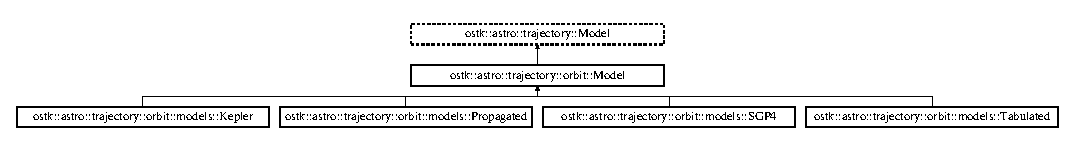
\includegraphics[height=1.484099cm]{classostk_1_1astro_1_1trajectory_1_1orbit_1_1_model}
\end{center}
\end{figure}
\doxysubsection*{Public Member Functions}
\begin{DoxyCompactItemize}
\item 
\mbox{\hyperlink{classostk_1_1astro_1_1trajectory_1_1orbit_1_1_model_a0604b5c1d0c0acb89cb42a10ea0fdb16}{Model}} ()
\item 
virtual \mbox{\hyperlink{classostk_1_1astro_1_1trajectory_1_1orbit_1_1_model_a7593c3eccd08104b00dd4d7c9c6a4d99}{$\sim$\+Model}} ()=0
\item 
virtual \mbox{\hyperlink{classostk_1_1astro_1_1trajectory_1_1orbit_1_1_model}{Model}} $\ast$ \mbox{\hyperlink{classostk_1_1astro_1_1trajectory_1_1orbit_1_1_model_a53dc07564e4c7c444da46360aa8ada15}{clone}} () const =0
\item 
virtual bool \mbox{\hyperlink{classostk_1_1astro_1_1trajectory_1_1orbit_1_1_model_a13c5b5693dd86a072da0bd0e319bacc2}{is\+Defined}} () const =0
\item 
virtual Instant \mbox{\hyperlink{classostk_1_1astro_1_1trajectory_1_1orbit_1_1_model_a22055d5ab4c22e6177a3ddb8f45f1f9b}{get\+Epoch}} () const =0
\item 
virtual Integer \mbox{\hyperlink{classostk_1_1astro_1_1trajectory_1_1orbit_1_1_model_af3f1866f86045da2c05efe4165735cf4}{get\+Revolution\+Number\+At\+Epoch}} () const =0
\item 
virtual \mbox{\hyperlink{classostk_1_1astro_1_1trajectory_1_1_state}{State}} \mbox{\hyperlink{classostk_1_1astro_1_1trajectory_1_1orbit_1_1_model_a34a0d8979ec1f7ade3e434fc0dad3711}{calculate\+State\+At}} (const Instant \&an\+Instant) const =0
\item 
virtual Integer \mbox{\hyperlink{classostk_1_1astro_1_1trajectory_1_1orbit_1_1_model_aeecf4cc22fa9c766801936c468cc52ac}{calculate\+Revolution\+Number\+At}} (const Instant \&an\+Instant) const =0
\item 
virtual void \mbox{\hyperlink{classostk_1_1astro_1_1trajectory_1_1orbit_1_1_model_a8ea45c1a6e51a6153ce3f72f5294f0c6}{print}} (std\+::ostream \&an\+Output\+Stream, bool display\+Decorator=true) const =0
\end{DoxyCompactItemize}


\doxysubsection{Constructor \& Destructor Documentation}
\mbox{\Hypertarget{classostk_1_1astro_1_1trajectory_1_1orbit_1_1_model_a0604b5c1d0c0acb89cb42a10ea0fdb16}\label{classostk_1_1astro_1_1trajectory_1_1orbit_1_1_model_a0604b5c1d0c0acb89cb42a10ea0fdb16}} 
\index{ostk::astro::trajectory::orbit::Model@{ostk::astro::trajectory::orbit::Model}!Model@{Model}}
\index{Model@{Model}!ostk::astro::trajectory::orbit::Model@{ostk::astro::trajectory::orbit::Model}}
\doxysubsubsection{\texorpdfstring{Model()}{Model()}}
{\footnotesize\ttfamily ostk\+::astro\+::trajectory\+::orbit\+::\+Model\+::\+Model (\begin{DoxyParamCaption}{ }\end{DoxyParamCaption})}

\mbox{\Hypertarget{classostk_1_1astro_1_1trajectory_1_1orbit_1_1_model_a7593c3eccd08104b00dd4d7c9c6a4d99}\label{classostk_1_1astro_1_1trajectory_1_1orbit_1_1_model_a7593c3eccd08104b00dd4d7c9c6a4d99}} 
\index{ostk::astro::trajectory::orbit::Model@{ostk::astro::trajectory::orbit::Model}!````~Model@{$\sim$Model}}
\index{````~Model@{$\sim$Model}!ostk::astro::trajectory::orbit::Model@{ostk::astro::trajectory::orbit::Model}}
\doxysubsubsection{\texorpdfstring{$\sim$Model()}{~Model()}}
{\footnotesize\ttfamily ostk\+::astro\+::trajectory\+::orbit\+::\+Model\+::$\sim$\+Model (\begin{DoxyParamCaption}{ }\end{DoxyParamCaption})\hspace{0.3cm}{\ttfamily [pure virtual]}}



Implements \mbox{\hyperlink{classostk_1_1astro_1_1trajectory_1_1_model_a23acd7acccf729d8343180b83fe2f9f9}{ostk\+::astro\+::trajectory\+::\+Model}}.



\doxysubsection{Member Function Documentation}
\mbox{\Hypertarget{classostk_1_1astro_1_1trajectory_1_1orbit_1_1_model_aeecf4cc22fa9c766801936c468cc52ac}\label{classostk_1_1astro_1_1trajectory_1_1orbit_1_1_model_aeecf4cc22fa9c766801936c468cc52ac}} 
\index{ostk::astro::trajectory::orbit::Model@{ostk::astro::trajectory::orbit::Model}!calculateRevolutionNumberAt@{calculateRevolutionNumberAt}}
\index{calculateRevolutionNumberAt@{calculateRevolutionNumberAt}!ostk::astro::trajectory::orbit::Model@{ostk::astro::trajectory::orbit::Model}}
\doxysubsubsection{\texorpdfstring{calculateRevolutionNumberAt()}{calculateRevolutionNumberAt()}}
{\footnotesize\ttfamily virtual Integer ostk\+::astro\+::trajectory\+::orbit\+::\+Model\+::calculate\+Revolution\+Number\+At (\begin{DoxyParamCaption}\item[{const Instant \&}]{an\+Instant }\end{DoxyParamCaption}) const\hspace{0.3cm}{\ttfamily [pure virtual]}}



Implemented in \mbox{\hyperlink{classostk_1_1astro_1_1trajectory_1_1orbit_1_1models_1_1_propagated_a6360392c65494aa42aadff58ec58e49c}{ostk\+::astro\+::trajectory\+::orbit\+::models\+::\+Propagated}}, \mbox{\hyperlink{classostk_1_1astro_1_1trajectory_1_1orbit_1_1models_1_1_kepler_a312fe4296eadcb00799ce9981b0c4f18}{ostk\+::astro\+::trajectory\+::orbit\+::models\+::\+Kepler}}, \mbox{\hyperlink{classostk_1_1astro_1_1trajectory_1_1orbit_1_1models_1_1_s_g_p4_af14e7851024d96eb20033ca9296dc003}{ostk\+::astro\+::trajectory\+::orbit\+::models\+::\+S\+G\+P4}}, and \mbox{\hyperlink{classostk_1_1astro_1_1trajectory_1_1orbit_1_1models_1_1_tabulated_ad7aabd8943ffaa16e569e331bdfa414e}{ostk\+::astro\+::trajectory\+::orbit\+::models\+::\+Tabulated}}.

\mbox{\Hypertarget{classostk_1_1astro_1_1trajectory_1_1orbit_1_1_model_a34a0d8979ec1f7ade3e434fc0dad3711}\label{classostk_1_1astro_1_1trajectory_1_1orbit_1_1_model_a34a0d8979ec1f7ade3e434fc0dad3711}} 
\index{ostk::astro::trajectory::orbit::Model@{ostk::astro::trajectory::orbit::Model}!calculateStateAt@{calculateStateAt}}
\index{calculateStateAt@{calculateStateAt}!ostk::astro::trajectory::orbit::Model@{ostk::astro::trajectory::orbit::Model}}
\doxysubsubsection{\texorpdfstring{calculateStateAt()}{calculateStateAt()}}
{\footnotesize\ttfamily virtual \mbox{\hyperlink{classostk_1_1astro_1_1trajectory_1_1_state}{State}} ostk\+::astro\+::trajectory\+::orbit\+::\+Model\+::calculate\+State\+At (\begin{DoxyParamCaption}\item[{const Instant \&}]{an\+Instant }\end{DoxyParamCaption}) const\hspace{0.3cm}{\ttfamily [pure virtual]}}



Implements \mbox{\hyperlink{classostk_1_1astro_1_1trajectory_1_1_model_ad25eeaded2946bf73d44161b5f4e9a0e}{ostk\+::astro\+::trajectory\+::\+Model}}.



Implemented in \mbox{\hyperlink{classostk_1_1astro_1_1trajectory_1_1orbit_1_1models_1_1_propagated_a2efc3c1af735dcf2ec622d056fa0a13f}{ostk\+::astro\+::trajectory\+::orbit\+::models\+::\+Propagated}}, \mbox{\hyperlink{classostk_1_1astro_1_1trajectory_1_1orbit_1_1models_1_1_kepler_a4de0c3d7a2b37c1c2ab4d6e207339809}{ostk\+::astro\+::trajectory\+::orbit\+::models\+::\+Kepler}}, \mbox{\hyperlink{classostk_1_1astro_1_1trajectory_1_1orbit_1_1models_1_1_s_g_p4_ad88439d9c46a75d3da8c20d2872271e3}{ostk\+::astro\+::trajectory\+::orbit\+::models\+::\+S\+G\+P4}}, and \mbox{\hyperlink{classostk_1_1astro_1_1trajectory_1_1orbit_1_1models_1_1_tabulated_ad7935cafe71b572b97b9df93e469d2f8}{ostk\+::astro\+::trajectory\+::orbit\+::models\+::\+Tabulated}}.

\mbox{\Hypertarget{classostk_1_1astro_1_1trajectory_1_1orbit_1_1_model_a53dc07564e4c7c444da46360aa8ada15}\label{classostk_1_1astro_1_1trajectory_1_1orbit_1_1_model_a53dc07564e4c7c444da46360aa8ada15}} 
\index{ostk::astro::trajectory::orbit::Model@{ostk::astro::trajectory::orbit::Model}!clone@{clone}}
\index{clone@{clone}!ostk::astro::trajectory::orbit::Model@{ostk::astro::trajectory::orbit::Model}}
\doxysubsubsection{\texorpdfstring{clone()}{clone()}}
{\footnotesize\ttfamily virtual \mbox{\hyperlink{classostk_1_1astro_1_1trajectory_1_1orbit_1_1_model}{Model}}$\ast$ ostk\+::astro\+::trajectory\+::orbit\+::\+Model\+::clone (\begin{DoxyParamCaption}{ }\end{DoxyParamCaption}) const\hspace{0.3cm}{\ttfamily [pure virtual]}}



Implements \mbox{\hyperlink{classostk_1_1astro_1_1trajectory_1_1_model_ad9f1467f711b07796ddc1437fb9ad9df}{ostk\+::astro\+::trajectory\+::\+Model}}.



Implemented in \mbox{\hyperlink{classostk_1_1astro_1_1trajectory_1_1orbit_1_1models_1_1_kepler_afb76b3571c73fb5c87129033f7d66520}{ostk\+::astro\+::trajectory\+::orbit\+::models\+::\+Kepler}}, \mbox{\hyperlink{classostk_1_1astro_1_1trajectory_1_1orbit_1_1models_1_1_propagated_a283639d985495c05adb9e80edb91cd12}{ostk\+::astro\+::trajectory\+::orbit\+::models\+::\+Propagated}}, \mbox{\hyperlink{classostk_1_1astro_1_1trajectory_1_1orbit_1_1models_1_1_s_g_p4_afb9928e09d66c13a77eb1126da6139eb}{ostk\+::astro\+::trajectory\+::orbit\+::models\+::\+S\+G\+P4}}, and \mbox{\hyperlink{classostk_1_1astro_1_1trajectory_1_1orbit_1_1models_1_1_tabulated_a53603727c33f9ff8db520831cf666142}{ostk\+::astro\+::trajectory\+::orbit\+::models\+::\+Tabulated}}.

\mbox{\Hypertarget{classostk_1_1astro_1_1trajectory_1_1orbit_1_1_model_a22055d5ab4c22e6177a3ddb8f45f1f9b}\label{classostk_1_1astro_1_1trajectory_1_1orbit_1_1_model_a22055d5ab4c22e6177a3ddb8f45f1f9b}} 
\index{ostk::astro::trajectory::orbit::Model@{ostk::astro::trajectory::orbit::Model}!getEpoch@{getEpoch}}
\index{getEpoch@{getEpoch}!ostk::astro::trajectory::orbit::Model@{ostk::astro::trajectory::orbit::Model}}
\doxysubsubsection{\texorpdfstring{getEpoch()}{getEpoch()}}
{\footnotesize\ttfamily virtual Instant ostk\+::astro\+::trajectory\+::orbit\+::\+Model\+::get\+Epoch (\begin{DoxyParamCaption}{ }\end{DoxyParamCaption}) const\hspace{0.3cm}{\ttfamily [pure virtual]}}



Implemented in \mbox{\hyperlink{classostk_1_1astro_1_1trajectory_1_1orbit_1_1models_1_1_propagated_a3bf49ac0824e10057b6abca2cfcc692f}{ostk\+::astro\+::trajectory\+::orbit\+::models\+::\+Propagated}}, \mbox{\hyperlink{classostk_1_1astro_1_1trajectory_1_1orbit_1_1models_1_1_kepler_a01551fd006896966d4d5e4442c182f92}{ostk\+::astro\+::trajectory\+::orbit\+::models\+::\+Kepler}}, \mbox{\hyperlink{classostk_1_1astro_1_1trajectory_1_1orbit_1_1models_1_1_s_g_p4_af577ee4ad56452fe510d325a61a9792e}{ostk\+::astro\+::trajectory\+::orbit\+::models\+::\+S\+G\+P4}}, and \mbox{\hyperlink{classostk_1_1astro_1_1trajectory_1_1orbit_1_1models_1_1_tabulated_a0e92ebaac60e5113989eaadc66062b75}{ostk\+::astro\+::trajectory\+::orbit\+::models\+::\+Tabulated}}.

\mbox{\Hypertarget{classostk_1_1astro_1_1trajectory_1_1orbit_1_1_model_af3f1866f86045da2c05efe4165735cf4}\label{classostk_1_1astro_1_1trajectory_1_1orbit_1_1_model_af3f1866f86045da2c05efe4165735cf4}} 
\index{ostk::astro::trajectory::orbit::Model@{ostk::astro::trajectory::orbit::Model}!getRevolutionNumberAtEpoch@{getRevolutionNumberAtEpoch}}
\index{getRevolutionNumberAtEpoch@{getRevolutionNumberAtEpoch}!ostk::astro::trajectory::orbit::Model@{ostk::astro::trajectory::orbit::Model}}
\doxysubsubsection{\texorpdfstring{getRevolutionNumberAtEpoch()}{getRevolutionNumberAtEpoch()}}
{\footnotesize\ttfamily virtual Integer ostk\+::astro\+::trajectory\+::orbit\+::\+Model\+::get\+Revolution\+Number\+At\+Epoch (\begin{DoxyParamCaption}{ }\end{DoxyParamCaption}) const\hspace{0.3cm}{\ttfamily [pure virtual]}}



Implemented in \mbox{\hyperlink{classostk_1_1astro_1_1trajectory_1_1orbit_1_1models_1_1_propagated_a789e4236d2b8b212b1d978055b76abf1}{ostk\+::astro\+::trajectory\+::orbit\+::models\+::\+Propagated}}, \mbox{\hyperlink{classostk_1_1astro_1_1trajectory_1_1orbit_1_1models_1_1_kepler_a2aa5b94462f65ea7e703d319d3e028b3}{ostk\+::astro\+::trajectory\+::orbit\+::models\+::\+Kepler}}, \mbox{\hyperlink{classostk_1_1astro_1_1trajectory_1_1orbit_1_1models_1_1_s_g_p4_a6216f01c1ee37817ca1ae1c7036f942c}{ostk\+::astro\+::trajectory\+::orbit\+::models\+::\+S\+G\+P4}}, and \mbox{\hyperlink{classostk_1_1astro_1_1trajectory_1_1orbit_1_1models_1_1_tabulated_adbd37f167e43cedcb15358c16d62bae8}{ostk\+::astro\+::trajectory\+::orbit\+::models\+::\+Tabulated}}.

\mbox{\Hypertarget{classostk_1_1astro_1_1trajectory_1_1orbit_1_1_model_a13c5b5693dd86a072da0bd0e319bacc2}\label{classostk_1_1astro_1_1trajectory_1_1orbit_1_1_model_a13c5b5693dd86a072da0bd0e319bacc2}} 
\index{ostk::astro::trajectory::orbit::Model@{ostk::astro::trajectory::orbit::Model}!isDefined@{isDefined}}
\index{isDefined@{isDefined}!ostk::astro::trajectory::orbit::Model@{ostk::astro::trajectory::orbit::Model}}
\doxysubsubsection{\texorpdfstring{isDefined()}{isDefined()}}
{\footnotesize\ttfamily virtual bool ostk\+::astro\+::trajectory\+::orbit\+::\+Model\+::is\+Defined (\begin{DoxyParamCaption}{ }\end{DoxyParamCaption}) const\hspace{0.3cm}{\ttfamily [pure virtual]}}



Implements \mbox{\hyperlink{classostk_1_1astro_1_1trajectory_1_1_model_a0d5cf6f754905f06c0ec1e39618c20a1}{ostk\+::astro\+::trajectory\+::\+Model}}.



Implemented in \mbox{\hyperlink{classostk_1_1astro_1_1trajectory_1_1orbit_1_1models_1_1_propagated_a530fd6bc017c74dedc43ced5fe843a03}{ostk\+::astro\+::trajectory\+::orbit\+::models\+::\+Propagated}}, \mbox{\hyperlink{classostk_1_1astro_1_1trajectory_1_1orbit_1_1models_1_1_kepler_a4c74402d5483a51e5e0fe1920cd52ec4}{ostk\+::astro\+::trajectory\+::orbit\+::models\+::\+Kepler}}, \mbox{\hyperlink{classostk_1_1astro_1_1trajectory_1_1orbit_1_1models_1_1_s_g_p4_ab18e0666588bd517c190942b1a54ed18}{ostk\+::astro\+::trajectory\+::orbit\+::models\+::\+S\+G\+P4}}, and \mbox{\hyperlink{classostk_1_1astro_1_1trajectory_1_1orbit_1_1models_1_1_tabulated_ad114ba4762b54211f74f0aa3ac5eedae}{ostk\+::astro\+::trajectory\+::orbit\+::models\+::\+Tabulated}}.

\mbox{\Hypertarget{classostk_1_1astro_1_1trajectory_1_1orbit_1_1_model_a8ea45c1a6e51a6153ce3f72f5294f0c6}\label{classostk_1_1astro_1_1trajectory_1_1orbit_1_1_model_a8ea45c1a6e51a6153ce3f72f5294f0c6}} 
\index{ostk::astro::trajectory::orbit::Model@{ostk::astro::trajectory::orbit::Model}!print@{print}}
\index{print@{print}!ostk::astro::trajectory::orbit::Model@{ostk::astro::trajectory::orbit::Model}}
\doxysubsubsection{\texorpdfstring{print()}{print()}}
{\footnotesize\ttfamily virtual void ostk\+::astro\+::trajectory\+::orbit\+::\+Model\+::print (\begin{DoxyParamCaption}\item[{std\+::ostream \&}]{an\+Output\+Stream,  }\item[{bool}]{display\+Decorator = {\ttfamily true} }\end{DoxyParamCaption}) const\hspace{0.3cm}{\ttfamily [pure virtual]}}



Implements \mbox{\hyperlink{classostk_1_1astro_1_1trajectory_1_1_model_a4b2098483430a820481ed50b81656e31}{ostk\+::astro\+::trajectory\+::\+Model}}.



Implemented in \mbox{\hyperlink{classostk_1_1astro_1_1trajectory_1_1orbit_1_1models_1_1_propagated_a2b8aa6ff5511dbe92e6a3e7f4dd6880b}{ostk\+::astro\+::trajectory\+::orbit\+::models\+::\+Propagated}}, \mbox{\hyperlink{classostk_1_1astro_1_1trajectory_1_1orbit_1_1models_1_1_kepler_a9c71803234f356ade03453e3ae19ae94}{ostk\+::astro\+::trajectory\+::orbit\+::models\+::\+Kepler}}, \mbox{\hyperlink{classostk_1_1astro_1_1trajectory_1_1orbit_1_1models_1_1_s_g_p4_a12416476201382c3d1e3c620f7be106a}{ostk\+::astro\+::trajectory\+::orbit\+::models\+::\+S\+G\+P4}}, and \mbox{\hyperlink{classostk_1_1astro_1_1trajectory_1_1orbit_1_1models_1_1_tabulated_a66be3f1f23a464c666c38a3adcc3bab5}{ostk\+::astro\+::trajectory\+::orbit\+::models\+::\+Tabulated}}.



The documentation for this class was generated from the following files\+:\begin{DoxyCompactItemize}
\item 
include/\+Open\+Space\+Toolkit/\+Astrodynamics/\+Trajectory/\+Orbit/\mbox{\hyperlink{_trajectory_2_orbit_2_model_8hpp}{Model.\+hpp}}\item 
src/\+Open\+Space\+Toolkit/\+Astrodynamics/\+Trajectory/\+Orbit/\mbox{\hyperlink{_trajectory_2_orbit_2_model_8cpp}{Model.\+cpp}}\end{DoxyCompactItemize}

\hypertarget{classostk_1_1astro_1_1_numerical_solver}{}\doxysection{ostk\+::astro\+::Numerical\+Solver Class Reference}
\label{classostk_1_1astro_1_1_numerical_solver}\index{ostk::astro::NumericalSolver@{ostk::astro::NumericalSolver}}


Defines a numerical O\+DE solver that use the Boost Odeint libraries. This class will be moved into O\+S\+Tk-\/math in the future.  




{\ttfamily \#include $<$Numerical\+Solver.\+hpp$>$}

\doxysubsection*{Classes}
\begin{DoxyCompactItemize}
\item 
struct \mbox{\hyperlink{structostk_1_1astro_1_1_numerical_solver_1_1_condition_solution}{Condition\+Solution}}
\end{DoxyCompactItemize}
\doxysubsection*{Public Types}
\begin{DoxyCompactItemize}
\item 
enum \mbox{\hyperlink{classostk_1_1astro_1_1_numerical_solver_afb80f81b2c3cc1d356b0b4749e45b947}{Stepper\+Type}} \{ \mbox{\hyperlink{classostk_1_1astro_1_1_numerical_solver_afb80f81b2c3cc1d356b0b4749e45b947a2ad1d4b322353ee07200045be21ffb58}{Stepper\+Type\+::\+Runge\+Kutta4}}, 
\mbox{\hyperlink{classostk_1_1astro_1_1_numerical_solver_afb80f81b2c3cc1d356b0b4749e45b947a646d9d3aaac989d6fd4990f308ba3a37}{Stepper\+Type\+::\+Runge\+Kutta\+Cash\+Karp54}}, 
\mbox{\hyperlink{classostk_1_1astro_1_1_numerical_solver_afb80f81b2c3cc1d356b0b4749e45b947a5002097811f3eb2dd4a34b826b1288e7}{Stepper\+Type\+::\+Runge\+Kutta\+Fehlberg78}}, 
\mbox{\hyperlink{classostk_1_1astro_1_1_numerical_solver_afb80f81b2c3cc1d356b0b4749e45b947a3203013d28f8e40a899ed45ede9ad149}{Stepper\+Type\+::\+Runge\+Kutta\+Dopri5}}
 \}
\item 
enum \mbox{\hyperlink{classostk_1_1astro_1_1_numerical_solver_a23e9e3f7d630f3097b4cbd91d9a2aa4c}{Log\+Type}} \{ \mbox{\hyperlink{classostk_1_1astro_1_1_numerical_solver_a23e9e3f7d630f3097b4cbd91d9a2aa4cac224e58a49e83bb9b94e2bd594fd5231}{Log\+Type\+::\+No\+Log}}, 
\mbox{\hyperlink{classostk_1_1astro_1_1_numerical_solver_a23e9e3f7d630f3097b4cbd91d9a2aa4ca40b79e6f53444b0a01aa353abfd9fe91}{Log\+Type\+::\+Log\+Constant}}, 
\mbox{\hyperlink{classostk_1_1astro_1_1_numerical_solver_a23e9e3f7d630f3097b4cbd91d9a2aa4caa412149ee02d5aaab7f9f710b2e39c5e}{Log\+Type\+::\+Log\+Adaptive}}
 \}
\item 
typedef Vector\+Xd \mbox{\hyperlink{classostk_1_1astro_1_1_numerical_solver_af91ffcd9d471c9fe3a093f9c5aa6f448}{State\+Vector}}
\item 
typedef Pair$<$ \mbox{\hyperlink{classostk_1_1astro_1_1_numerical_solver_af91ffcd9d471c9fe3a093f9c5aa6f448}{State\+Vector}}, double $>$ \mbox{\hyperlink{classostk_1_1astro_1_1_numerical_solver_af7ade38a233dbf4f3a59161aa87ecb77}{Solution}}
\item 
typedef std\+::function$<$ void(const \mbox{\hyperlink{classostk_1_1astro_1_1_numerical_solver_af91ffcd9d471c9fe3a093f9c5aa6f448}{State\+Vector}} \&, \mbox{\hyperlink{classostk_1_1astro_1_1_numerical_solver_af91ffcd9d471c9fe3a093f9c5aa6f448}{State\+Vector}} \&, const double)$>$ \mbox{\hyperlink{classostk_1_1astro_1_1_numerical_solver_aa39593aa5ff747e4f68492708b45bbc5}{System\+Of\+Equations\+Wrapper}}
\end{DoxyCompactItemize}
\doxysubsection*{Public Member Functions}
\begin{DoxyCompactItemize}
\item 
\mbox{\hyperlink{classostk_1_1astro_1_1_numerical_solver_a7ee8408e552fdf6173d9315c0e382359}{Numerical\+Solver}} (const \mbox{\hyperlink{classostk_1_1astro_1_1_numerical_solver_a23e9e3f7d630f3097b4cbd91d9a2aa4c}{Numerical\+Solver\+::\+Log\+Type}} \&a\+Log\+Type, const \mbox{\hyperlink{classostk_1_1astro_1_1_numerical_solver_afb80f81b2c3cc1d356b0b4749e45b947}{Numerical\+Solver\+::\+Stepper\+Type}} \&a\+Stepper\+Type, const Real \&a\+Time\+Step, const Real \&a\+Relative\+Tolerance, const Real \&an\+Absolute\+Tolerance, const \mbox{\hyperlink{classostk_1_1astro_1_1_root_solver}{Root\+Solver}} \&a\+Root\+Solver=\mbox{\hyperlink{classostk_1_1astro_1_1_root_solver_a1183671b30532b0b9096ab24e7c675f4}{Root\+Solver\+::\+Default}}())
\begin{DoxyCompactList}\small\item\em Constructor. \end{DoxyCompactList}\item 
\mbox{\hyperlink{classostk_1_1astro_1_1_numerical_solver}{Numerical\+Solver}} $\ast$ \mbox{\hyperlink{classostk_1_1astro_1_1_numerical_solver_a5b96baffe23b77c14046e4fb7ffc89a1}{clone}} () const
\begin{DoxyCompactList}\small\item\em Clone numerical solver. \end{DoxyCompactList}\item 
bool \mbox{\hyperlink{classostk_1_1astro_1_1_numerical_solver_a4ec848789b81d968cdc1d3d5003ea66a}{operator==}} (const \mbox{\hyperlink{classostk_1_1astro_1_1_numerical_solver}{Numerical\+Solver}} \&a\+Numerical\+Solver) const
\begin{DoxyCompactList}\small\item\em Equal to operator. \end{DoxyCompactList}\item 
bool \mbox{\hyperlink{classostk_1_1astro_1_1_numerical_solver_af488ebaa295739474e0f696aa9134171}{operator!=}} (const \mbox{\hyperlink{classostk_1_1astro_1_1_numerical_solver}{Numerical\+Solver}} \&a\+Numerical\+Solver) const
\begin{DoxyCompactList}\small\item\em Not equal to operator. \end{DoxyCompactList}\item 
bool \mbox{\hyperlink{classostk_1_1astro_1_1_numerical_solver_a936f93694a47c4ebca82fb6e233b8b4a}{is\+Defined}} () const
\begin{DoxyCompactList}\small\item\em Check if numerical solver is defined. \end{DoxyCompactList}\item 
void \mbox{\hyperlink{classostk_1_1astro_1_1_numerical_solver_a8572e8bc097feb35d7e7ba293ffd511a}{print}} (std\+::ostream \&an\+Output\+Stream, bool display\+Decorator=true) const
\begin{DoxyCompactList}\small\item\em Print numerical solver. \end{DoxyCompactList}\item 
\mbox{\hyperlink{classostk_1_1astro_1_1_numerical_solver_a23e9e3f7d630f3097b4cbd91d9a2aa4c}{Numerical\+Solver\+::\+Log\+Type}} \mbox{\hyperlink{classostk_1_1astro_1_1_numerical_solver_ad0403195d44325cc71a8a19359640329}{get\+Log\+Type}} () const
\begin{DoxyCompactList}\small\item\em Get integration logging enum. \end{DoxyCompactList}\item 
\mbox{\hyperlink{classostk_1_1astro_1_1_numerical_solver_afb80f81b2c3cc1d356b0b4749e45b947}{Numerical\+Solver\+::\+Stepper\+Type}} \mbox{\hyperlink{classostk_1_1astro_1_1_numerical_solver_adb327bb6a9dc0fc4ab8fca57030b51e6}{get\+Stepper\+Type}} () const
\begin{DoxyCompactList}\small\item\em Get integration stepper enum. \end{DoxyCompactList}\item 
Real \mbox{\hyperlink{classostk_1_1astro_1_1_numerical_solver_a1caf9f97b27630a5baa4444e76fe9ad4}{get\+Time\+Step}} () const
\begin{DoxyCompactList}\small\item\em Get initial time step guess. \end{DoxyCompactList}\item 
Real \mbox{\hyperlink{classostk_1_1astro_1_1_numerical_solver_acdd27776ff2d4fca2bb6cb4fbb94b547}{get\+Relative\+Tolerance}} () const
\begin{DoxyCompactList}\small\item\em Get relative integration tolerance. \end{DoxyCompactList}\item 
Real \mbox{\hyperlink{classostk_1_1astro_1_1_numerical_solver_a0f768255c5f2f51f395e4515db245930}{get\+Absolute\+Tolerance}} () const
\begin{DoxyCompactList}\small\item\em Get absolute integration tolerance. \end{DoxyCompactList}\item 
\mbox{\hyperlink{classostk_1_1astro_1_1_root_solver}{Root\+Solver}} \mbox{\hyperlink{classostk_1_1astro_1_1_numerical_solver_a22102966485304b7fad6c0dd793362c0}{get\+Root\+Solver}} () const
\begin{DoxyCompactList}\small\item\em Get root solver. \end{DoxyCompactList}\item 
Array$<$ \mbox{\hyperlink{classostk_1_1astro_1_1_numerical_solver_af7ade38a233dbf4f3a59161aa87ecb77}{Solution}} $>$ \mbox{\hyperlink{classostk_1_1astro_1_1_numerical_solver_aab4999a9a2b780ffc839eec7eb357fe3}{integrate\+Time}} (const \mbox{\hyperlink{classostk_1_1astro_1_1_numerical_solver_af91ffcd9d471c9fe3a093f9c5aa6f448}{State\+Vector}} \&an\+Initial\+State\+Vector, const Real \&a\+Start\+Time, const Array$<$ Real $>$ \&a\+Time\+Array, const \mbox{\hyperlink{classostk_1_1astro_1_1_numerical_solver_aa39593aa5ff747e4f68492708b45bbc5}{System\+Of\+Equations\+Wrapper}} \&a\+System\+Of\+Equations)
\begin{DoxyCompactList}\small\item\em Perform numerical integration from a start time to an array of times. \end{DoxyCompactList}\item 
\mbox{\hyperlink{classostk_1_1astro_1_1_numerical_solver_af7ade38a233dbf4f3a59161aa87ecb77}{Solution}} \mbox{\hyperlink{classostk_1_1astro_1_1_numerical_solver_ab3cd83c7f53ef794b9d69a2be35137e4}{integrate\+Time}} (const \mbox{\hyperlink{classostk_1_1astro_1_1_numerical_solver_af91ffcd9d471c9fe3a093f9c5aa6f448}{State\+Vector}} \&an\+Initial\+State\+Vector, const Real \&a\+Start\+Time, const Real \&an\+End\+Time, const \mbox{\hyperlink{classostk_1_1astro_1_1_numerical_solver_aa39593aa5ff747e4f68492708b45bbc5}{System\+Of\+Equations\+Wrapper}} \&a\+System\+Of\+Equations)
\begin{DoxyCompactList}\small\item\em Perform numerical integration from a start time to an end time. \end{DoxyCompactList}\item 
\mbox{\hyperlink{structostk_1_1astro_1_1_numerical_solver_1_1_condition_solution}{Condition\+Solution}} \mbox{\hyperlink{classostk_1_1astro_1_1_numerical_solver_aa9123455fb97853147c26c6c734b438c}{integrate\+Time}} (const \mbox{\hyperlink{classostk_1_1astro_1_1_numerical_solver_af91ffcd9d471c9fe3a093f9c5aa6f448}{State\+Vector}} \&an\+Initial\+State\+Vector, const Real \&a\+Start\+Time, const Real \&an\+End\+Time, const \mbox{\hyperlink{classostk_1_1astro_1_1_numerical_solver_aa39593aa5ff747e4f68492708b45bbc5}{System\+Of\+Equations\+Wrapper}} \&a\+System\+Of\+Equations, const \mbox{\hyperlink{classostk_1_1astro_1_1_event_condition}{Event\+Condition}} \&an\+Event\+Condition)
\begin{DoxyCompactList}\small\item\em Perform numerical integration from a start time until either a condition or the end time is reached. \end{DoxyCompactList}\item 
\mbox{\hyperlink{classostk_1_1astro_1_1_numerical_solver_af7ade38a233dbf4f3a59161aa87ecb77}{Solution}} \mbox{\hyperlink{classostk_1_1astro_1_1_numerical_solver_adde6e4f6648884ac27bc6a945fcdc298}{integrate\+Duration}} (const \mbox{\hyperlink{classostk_1_1astro_1_1_numerical_solver_af91ffcd9d471c9fe3a093f9c5aa6f448}{State\+Vector}} \&an\+Initial\+State\+Vector, const Real \&a\+Duration\+In\+Seconds, const \mbox{\hyperlink{classostk_1_1astro_1_1_numerical_solver_aa39593aa5ff747e4f68492708b45bbc5}{System\+Of\+Equations\+Wrapper}} \&a\+System\+Of\+Equations)
\begin{DoxyCompactList}\small\item\em Perform numerical integration for a specified duration. \end{DoxyCompactList}\item 
Array$<$ \mbox{\hyperlink{classostk_1_1astro_1_1_numerical_solver_af7ade38a233dbf4f3a59161aa87ecb77}{Solution}} $>$ \mbox{\hyperlink{classostk_1_1astro_1_1_numerical_solver_a269c7e91519287bba7e4cbc571646b3e}{integrate\+Duration}} (const \mbox{\hyperlink{classostk_1_1astro_1_1_numerical_solver_af91ffcd9d471c9fe3a093f9c5aa6f448}{State\+Vector}} \&an\+Initial\+State\+Vector, const Array$<$ Real $>$ \&a\+Duration\+Array, const \mbox{\hyperlink{classostk_1_1astro_1_1_numerical_solver_aa39593aa5ff747e4f68492708b45bbc5}{System\+Of\+Equations\+Wrapper}} \&a\+System\+Of\+Equations)
\begin{DoxyCompactList}\small\item\em Perform numerical integration for an array of durations. \end{DoxyCompactList}\item 
\mbox{\hyperlink{structostk_1_1astro_1_1_numerical_solver_1_1_condition_solution}{Condition\+Solution}} \mbox{\hyperlink{classostk_1_1astro_1_1_numerical_solver_ae1b3381e52aeeedbc8861d1936c6b876}{integrate\+Duration}} (const \mbox{\hyperlink{classostk_1_1astro_1_1_numerical_solver_af91ffcd9d471c9fe3a093f9c5aa6f448}{State\+Vector}} \&an\+Initial\+State\+Vector, const Real \&a\+Duration\+In\+Seconds, const \mbox{\hyperlink{classostk_1_1astro_1_1_numerical_solver_aa39593aa5ff747e4f68492708b45bbc5}{System\+Of\+Equations\+Wrapper}} \&a\+System\+Of\+Equations, const \mbox{\hyperlink{classostk_1_1astro_1_1_event_condition}{Event\+Condition}} \&an\+Event\+Condition)
\begin{DoxyCompactList}\small\item\em Perform numerical integration from a start time until either a condition or duration is met. \end{DoxyCompactList}\end{DoxyCompactItemize}
\doxysubsection*{Static Public Member Functions}
\begin{DoxyCompactItemize}
\item 
static String \mbox{\hyperlink{classostk_1_1astro_1_1_numerical_solver_a3dd4e9b6acffec931c3748d4d851155b}{String\+From\+Stepper\+Type}} (const \mbox{\hyperlink{classostk_1_1astro_1_1_numerical_solver_afb80f81b2c3cc1d356b0b4749e45b947}{Numerical\+Solver\+::\+Stepper\+Type}} \&a\+Stepper\+Type)
\begin{DoxyCompactList}\small\item\em Get string from the integration stepper type. \end{DoxyCompactList}\item 
static String \mbox{\hyperlink{classostk_1_1astro_1_1_numerical_solver_ab75ca02c5e4d0b2b2390045c353bf66f}{String\+From\+Log\+Type}} (const \mbox{\hyperlink{classostk_1_1astro_1_1_numerical_solver_a23e9e3f7d630f3097b4cbd91d9a2aa4c}{Numerical\+Solver\+::\+Log\+Type}} \&a\+Log\+Type)
\begin{DoxyCompactList}\small\item\em Get string from the integration log type. \end{DoxyCompactList}\item 
static \mbox{\hyperlink{classostk_1_1astro_1_1_numerical_solver}{Numerical\+Solver}} \mbox{\hyperlink{classostk_1_1astro_1_1_numerical_solver_ae58ebf25a5d10efd91b4a5d48ec8aedb}{Undefined}} ()
\begin{DoxyCompactList}\small\item\em Undefined. \end{DoxyCompactList}\item 
static \mbox{\hyperlink{classostk_1_1astro_1_1_numerical_solver}{Numerical\+Solver}} \mbox{\hyperlink{classostk_1_1astro_1_1_numerical_solver_a5fe1ae5cb8e96de77736af980ce11ec8}{Default}} ()
\begin{DoxyCompactList}\small\item\em Default. \end{DoxyCompactList}\end{DoxyCompactItemize}
\doxysubsection*{Friends}
\begin{DoxyCompactItemize}
\item 
std\+::ostream \& \mbox{\hyperlink{classostk_1_1astro_1_1_numerical_solver_a28e4d7a66856d0bedb035589eb5e70f7}{operator$<$$<$}} (std\+::ostream \&an\+Output\+Stream, const \mbox{\hyperlink{classostk_1_1astro_1_1_numerical_solver}{Numerical\+Solver}} \&a\+Numerical\+Solver)
\begin{DoxyCompactList}\small\item\em Output stream operator. \end{DoxyCompactList}\end{DoxyCompactItemize}


\doxysubsection{Detailed Description}
Defines a numerical O\+DE solver that use the Boost Odeint libraries. This class will be moved into O\+S\+Tk-\/math in the future. 

\doxysubsection{Member Typedef Documentation}
\mbox{\Hypertarget{classostk_1_1astro_1_1_numerical_solver_af7ade38a233dbf4f3a59161aa87ecb77}\label{classostk_1_1astro_1_1_numerical_solver_af7ade38a233dbf4f3a59161aa87ecb77}} 
\index{ostk::astro::NumericalSolver@{ostk::astro::NumericalSolver}!Solution@{Solution}}
\index{Solution@{Solution}!ostk::astro::NumericalSolver@{ostk::astro::NumericalSolver}}
\doxysubsubsection{\texorpdfstring{Solution}{Solution}}
{\footnotesize\ttfamily typedef Pair$<$\mbox{\hyperlink{classostk_1_1astro_1_1_numerical_solver_af91ffcd9d471c9fe3a093f9c5aa6f448}{State\+Vector}}, double$>$ \mbox{\hyperlink{classostk_1_1astro_1_1_numerical_solver_af7ade38a233dbf4f3a59161aa87ecb77}{ostk\+::astro\+::\+Numerical\+Solver\+::\+Solution}}}

\mbox{\Hypertarget{classostk_1_1astro_1_1_numerical_solver_af91ffcd9d471c9fe3a093f9c5aa6f448}\label{classostk_1_1astro_1_1_numerical_solver_af91ffcd9d471c9fe3a093f9c5aa6f448}} 
\index{ostk::astro::NumericalSolver@{ostk::astro::NumericalSolver}!StateVector@{StateVector}}
\index{StateVector@{StateVector}!ostk::astro::NumericalSolver@{ostk::astro::NumericalSolver}}
\doxysubsubsection{\texorpdfstring{StateVector}{StateVector}}
{\footnotesize\ttfamily typedef Vector\+Xd \mbox{\hyperlink{classostk_1_1astro_1_1_numerical_solver_af91ffcd9d471c9fe3a093f9c5aa6f448}{ostk\+::astro\+::\+Numerical\+Solver\+::\+State\+Vector}}}

\mbox{\Hypertarget{classostk_1_1astro_1_1_numerical_solver_aa39593aa5ff747e4f68492708b45bbc5}\label{classostk_1_1astro_1_1_numerical_solver_aa39593aa5ff747e4f68492708b45bbc5}} 
\index{ostk::astro::NumericalSolver@{ostk::astro::NumericalSolver}!SystemOfEquationsWrapper@{SystemOfEquationsWrapper}}
\index{SystemOfEquationsWrapper@{SystemOfEquationsWrapper}!ostk::astro::NumericalSolver@{ostk::astro::NumericalSolver}}
\doxysubsubsection{\texorpdfstring{SystemOfEquationsWrapper}{SystemOfEquationsWrapper}}
{\footnotesize\ttfamily typedef std\+::function$<$void(const \mbox{\hyperlink{classostk_1_1astro_1_1_numerical_solver_af91ffcd9d471c9fe3a093f9c5aa6f448}{State\+Vector}}\&, \mbox{\hyperlink{classostk_1_1astro_1_1_numerical_solver_af91ffcd9d471c9fe3a093f9c5aa6f448}{State\+Vector}}\&, const double)$>$ \mbox{\hyperlink{classostk_1_1astro_1_1_numerical_solver_aa39593aa5ff747e4f68492708b45bbc5}{ostk\+::astro\+::\+Numerical\+Solver\+::\+System\+Of\+Equations\+Wrapper}}}



\doxysubsection{Member Enumeration Documentation}
\mbox{\Hypertarget{classostk_1_1astro_1_1_numerical_solver_a23e9e3f7d630f3097b4cbd91d9a2aa4c}\label{classostk_1_1astro_1_1_numerical_solver_a23e9e3f7d630f3097b4cbd91d9a2aa4c}} 
\index{ostk::astro::NumericalSolver@{ostk::astro::NumericalSolver}!LogType@{LogType}}
\index{LogType@{LogType}!ostk::astro::NumericalSolver@{ostk::astro::NumericalSolver}}
\doxysubsubsection{\texorpdfstring{LogType}{LogType}}
{\footnotesize\ttfamily enum \mbox{\hyperlink{classostk_1_1astro_1_1_numerical_solver_a23e9e3f7d630f3097b4cbd91d9a2aa4c}{ostk\+::astro\+::\+Numerical\+Solver\+::\+Log\+Type}}\hspace{0.3cm}{\ttfamily [strong]}}

\begin{DoxyEnumFields}{Enumerator}
\raisebox{\heightof{T}}[0pt][0pt]{\index{NoLog@{NoLog}!ostk::astro::NumericalSolver@{ostk::astro::NumericalSolver}}\index{ostk::astro::NumericalSolver@{ostk::astro::NumericalSolver}!NoLog@{NoLog}}}\mbox{\Hypertarget{classostk_1_1astro_1_1_numerical_solver_a23e9e3f7d630f3097b4cbd91d9a2aa4cac224e58a49e83bb9b94e2bd594fd5231}\label{classostk_1_1astro_1_1_numerical_solver_a23e9e3f7d630f3097b4cbd91d9a2aa4cac224e58a49e83bb9b94e2bd594fd5231}} 
No\+Log&\\
\hline

\raisebox{\heightof{T}}[0pt][0pt]{\index{LogConstant@{LogConstant}!ostk::astro::NumericalSolver@{ostk::astro::NumericalSolver}}\index{ostk::astro::NumericalSolver@{ostk::astro::NumericalSolver}!LogConstant@{LogConstant}}}\mbox{\Hypertarget{classostk_1_1astro_1_1_numerical_solver_a23e9e3f7d630f3097b4cbd91d9a2aa4ca40b79e6f53444b0a01aa353abfd9fe91}\label{classostk_1_1astro_1_1_numerical_solver_a23e9e3f7d630f3097b4cbd91d9a2aa4ca40b79e6f53444b0a01aa353abfd9fe91}} 
Log\+Constant&\\
\hline

\raisebox{\heightof{T}}[0pt][0pt]{\index{LogAdaptive@{LogAdaptive}!ostk::astro::NumericalSolver@{ostk::astro::NumericalSolver}}\index{ostk::astro::NumericalSolver@{ostk::astro::NumericalSolver}!LogAdaptive@{LogAdaptive}}}\mbox{\Hypertarget{classostk_1_1astro_1_1_numerical_solver_a23e9e3f7d630f3097b4cbd91d9a2aa4caa412149ee02d5aaab7f9f710b2e39c5e}\label{classostk_1_1astro_1_1_numerical_solver_a23e9e3f7d630f3097b4cbd91d9a2aa4caa412149ee02d5aaab7f9f710b2e39c5e}} 
Log\+Adaptive&\\
\hline

\end{DoxyEnumFields}
\mbox{\Hypertarget{classostk_1_1astro_1_1_numerical_solver_afb80f81b2c3cc1d356b0b4749e45b947}\label{classostk_1_1astro_1_1_numerical_solver_afb80f81b2c3cc1d356b0b4749e45b947}} 
\index{ostk::astro::NumericalSolver@{ostk::astro::NumericalSolver}!StepperType@{StepperType}}
\index{StepperType@{StepperType}!ostk::astro::NumericalSolver@{ostk::astro::NumericalSolver}}
\doxysubsubsection{\texorpdfstring{StepperType}{StepperType}}
{\footnotesize\ttfamily enum \mbox{\hyperlink{classostk_1_1astro_1_1_numerical_solver_afb80f81b2c3cc1d356b0b4749e45b947}{ostk\+::astro\+::\+Numerical\+Solver\+::\+Stepper\+Type}}\hspace{0.3cm}{\ttfamily [strong]}}

\begin{DoxyEnumFields}{Enumerator}
\raisebox{\heightof{T}}[0pt][0pt]{\index{RungeKutta4@{RungeKutta4}!ostk::astro::NumericalSolver@{ostk::astro::NumericalSolver}}\index{ostk::astro::NumericalSolver@{ostk::astro::NumericalSolver}!RungeKutta4@{RungeKutta4}}}\mbox{\Hypertarget{classostk_1_1astro_1_1_numerical_solver_afb80f81b2c3cc1d356b0b4749e45b947a2ad1d4b322353ee07200045be21ffb58}\label{classostk_1_1astro_1_1_numerical_solver_afb80f81b2c3cc1d356b0b4749e45b947a2ad1d4b322353ee07200045be21ffb58}} 
Runge\+Kutta4&\\
\hline

\raisebox{\heightof{T}}[0pt][0pt]{\index{RungeKuttaCashKarp54@{RungeKuttaCashKarp54}!ostk::astro::NumericalSolver@{ostk::astro::NumericalSolver}}\index{ostk::astro::NumericalSolver@{ostk::astro::NumericalSolver}!RungeKuttaCashKarp54@{RungeKuttaCashKarp54}}}\mbox{\Hypertarget{classostk_1_1astro_1_1_numerical_solver_afb80f81b2c3cc1d356b0b4749e45b947a646d9d3aaac989d6fd4990f308ba3a37}\label{classostk_1_1astro_1_1_numerical_solver_afb80f81b2c3cc1d356b0b4749e45b947a646d9d3aaac989d6fd4990f308ba3a37}} 
Runge\+Kutta\+Cash\+Karp54&\\
\hline

\raisebox{\heightof{T}}[0pt][0pt]{\index{RungeKuttaFehlberg78@{RungeKuttaFehlberg78}!ostk::astro::NumericalSolver@{ostk::astro::NumericalSolver}}\index{ostk::astro::NumericalSolver@{ostk::astro::NumericalSolver}!RungeKuttaFehlberg78@{RungeKuttaFehlberg78}}}\mbox{\Hypertarget{classostk_1_1astro_1_1_numerical_solver_afb80f81b2c3cc1d356b0b4749e45b947a5002097811f3eb2dd4a34b826b1288e7}\label{classostk_1_1astro_1_1_numerical_solver_afb80f81b2c3cc1d356b0b4749e45b947a5002097811f3eb2dd4a34b826b1288e7}} 
Runge\+Kutta\+Fehlberg78&\\
\hline

\raisebox{\heightof{T}}[0pt][0pt]{\index{RungeKuttaDopri5@{RungeKuttaDopri5}!ostk::astro::NumericalSolver@{ostk::astro::NumericalSolver}}\index{ostk::astro::NumericalSolver@{ostk::astro::NumericalSolver}!RungeKuttaDopri5@{RungeKuttaDopri5}}}\mbox{\Hypertarget{classostk_1_1astro_1_1_numerical_solver_afb80f81b2c3cc1d356b0b4749e45b947a3203013d28f8e40a899ed45ede9ad149}\label{classostk_1_1astro_1_1_numerical_solver_afb80f81b2c3cc1d356b0b4749e45b947a3203013d28f8e40a899ed45ede9ad149}} 
Runge\+Kutta\+Dopri5&\\
\hline

\end{DoxyEnumFields}


\doxysubsection{Constructor \& Destructor Documentation}
\mbox{\Hypertarget{classostk_1_1astro_1_1_numerical_solver_a7ee8408e552fdf6173d9315c0e382359}\label{classostk_1_1astro_1_1_numerical_solver_a7ee8408e552fdf6173d9315c0e382359}} 
\index{ostk::astro::NumericalSolver@{ostk::astro::NumericalSolver}!NumericalSolver@{NumericalSolver}}
\index{NumericalSolver@{NumericalSolver}!ostk::astro::NumericalSolver@{ostk::astro::NumericalSolver}}
\doxysubsubsection{\texorpdfstring{NumericalSolver()}{NumericalSolver()}}
{\footnotesize\ttfamily ostk\+::astro\+::\+Numerical\+Solver\+::\+Numerical\+Solver (\begin{DoxyParamCaption}\item[{const \mbox{\hyperlink{classostk_1_1astro_1_1_numerical_solver_a23e9e3f7d630f3097b4cbd91d9a2aa4c}{Numerical\+Solver\+::\+Log\+Type}} \&}]{a\+Log\+Type,  }\item[{const \mbox{\hyperlink{classostk_1_1astro_1_1_numerical_solver_afb80f81b2c3cc1d356b0b4749e45b947}{Numerical\+Solver\+::\+Stepper\+Type}} \&}]{a\+Stepper\+Type,  }\item[{const Real \&}]{a\+Time\+Step,  }\item[{const Real \&}]{a\+Relative\+Tolerance,  }\item[{const Real \&}]{an\+Absolute\+Tolerance,  }\item[{const \mbox{\hyperlink{classostk_1_1astro_1_1_root_solver}{Root\+Solver}} \&}]{a\+Root\+Solver = {\ttfamily \mbox{\hyperlink{classostk_1_1astro_1_1_root_solver_a1183671b30532b0b9096ab24e7c675f4}{Root\+Solver\+::\+Default}}()} }\end{DoxyParamCaption})}



Constructor. 


\begin{DoxyCode}{0}
\DoxyCodeLine{\mbox{\hyperlink{classostk_1_1astro_1_1_numerical_solver_a7ee8408e552fdf6173d9315c0e382359}{NumericalSolver}} numericalSolver = \{ aLogType, aStepperType, aTimeStep,}
\DoxyCodeLine{aRelativeTolerance, anAbsoluteTolerance \} ;}
\end{DoxyCode}



\begin{DoxyParams}[1]{Parameters}
\mbox{\texttt{ in}}  & {\em a\+Log\+Type} & An enum indicating the amount of verbosity wanted to be logged during numerical integration \\
\hline
\mbox{\texttt{ in}}  & {\em a\+Stepper\+Type} & An enum indicating the type of numerical stepper used to perform integration \\
\hline
\mbox{\texttt{ in}}  & {\em a\+Time\+Step} & A number indicating the initial guess time step the numerical solver will take \\
\hline
\mbox{\texttt{ in}}  & {\em a\+Relative\+Tolerance} & A number indicating the relative integration tolerance \\
\hline
\mbox{\texttt{ in}}  & {\em an\+Absolute\+Tolerance} & A number indicating the absolute integration tolerance \\
\hline
\end{DoxyParams}


\doxysubsection{Member Function Documentation}
\mbox{\Hypertarget{classostk_1_1astro_1_1_numerical_solver_a5b96baffe23b77c14046e4fb7ffc89a1}\label{classostk_1_1astro_1_1_numerical_solver_a5b96baffe23b77c14046e4fb7ffc89a1}} 
\index{ostk::astro::NumericalSolver@{ostk::astro::NumericalSolver}!clone@{clone}}
\index{clone@{clone}!ostk::astro::NumericalSolver@{ostk::astro::NumericalSolver}}
\doxysubsubsection{\texorpdfstring{clone()}{clone()}}
{\footnotesize\ttfamily \mbox{\hyperlink{classostk_1_1astro_1_1_numerical_solver}{Numerical\+Solver}} $\ast$ ostk\+::astro\+::\+Numerical\+Solver\+::clone (\begin{DoxyParamCaption}{ }\end{DoxyParamCaption}) const}



Clone numerical solver. 

\begin{DoxyReturn}{Returns}
Pointer to cloned numerical solver 
\end{DoxyReturn}
\mbox{\Hypertarget{classostk_1_1astro_1_1_numerical_solver_a5fe1ae5cb8e96de77736af980ce11ec8}\label{classostk_1_1astro_1_1_numerical_solver_a5fe1ae5cb8e96de77736af980ce11ec8}} 
\index{ostk::astro::NumericalSolver@{ostk::astro::NumericalSolver}!Default@{Default}}
\index{Default@{Default}!ostk::astro::NumericalSolver@{ostk::astro::NumericalSolver}}
\doxysubsubsection{\texorpdfstring{Default()}{Default()}}
{\footnotesize\ttfamily \mbox{\hyperlink{classostk_1_1astro_1_1_numerical_solver}{Numerical\+Solver}} ostk\+::astro\+::\+Numerical\+Solver\+::\+Default (\begin{DoxyParamCaption}{ }\end{DoxyParamCaption})\hspace{0.3cm}{\ttfamily [static]}}



Default. 

\begin{DoxyReturn}{Returns}
A default numerical solver 
\end{DoxyReturn}
\mbox{\Hypertarget{classostk_1_1astro_1_1_numerical_solver_a0f768255c5f2f51f395e4515db245930}\label{classostk_1_1astro_1_1_numerical_solver_a0f768255c5f2f51f395e4515db245930}} 
\index{ostk::astro::NumericalSolver@{ostk::astro::NumericalSolver}!getAbsoluteTolerance@{getAbsoluteTolerance}}
\index{getAbsoluteTolerance@{getAbsoluteTolerance}!ostk::astro::NumericalSolver@{ostk::astro::NumericalSolver}}
\doxysubsubsection{\texorpdfstring{getAbsoluteTolerance()}{getAbsoluteTolerance()}}
{\footnotesize\ttfamily Real ostk\+::astro\+::\+Numerical\+Solver\+::get\+Absolute\+Tolerance (\begin{DoxyParamCaption}{ }\end{DoxyParamCaption}) const}



Get absolute integration tolerance. 


\begin{DoxyCode}{0}
\DoxyCodeLine{numericalSolver.getAbsoluteTolerance() ;}
\end{DoxyCode}


\begin{DoxyReturn}{Returns}
Real 
\end{DoxyReturn}
\mbox{\Hypertarget{classostk_1_1astro_1_1_numerical_solver_ad0403195d44325cc71a8a19359640329}\label{classostk_1_1astro_1_1_numerical_solver_ad0403195d44325cc71a8a19359640329}} 
\index{ostk::astro::NumericalSolver@{ostk::astro::NumericalSolver}!getLogType@{getLogType}}
\index{getLogType@{getLogType}!ostk::astro::NumericalSolver@{ostk::astro::NumericalSolver}}
\doxysubsubsection{\texorpdfstring{getLogType()}{getLogType()}}
{\footnotesize\ttfamily \mbox{\hyperlink{classostk_1_1astro_1_1_numerical_solver_a23e9e3f7d630f3097b4cbd91d9a2aa4c}{Numerical\+Solver\+::\+Log\+Type}} ostk\+::astro\+::\+Numerical\+Solver\+::get\+Log\+Type (\begin{DoxyParamCaption}{ }\end{DoxyParamCaption}) const}



Get integration logging enum. 


\begin{DoxyCode}{0}
\DoxyCodeLine{numericalSolver.getLogType() ;}
\end{DoxyCode}


\begin{DoxyReturn}{Returns}
Log\+Type 
\end{DoxyReturn}
\mbox{\Hypertarget{classostk_1_1astro_1_1_numerical_solver_acdd27776ff2d4fca2bb6cb4fbb94b547}\label{classostk_1_1astro_1_1_numerical_solver_acdd27776ff2d4fca2bb6cb4fbb94b547}} 
\index{ostk::astro::NumericalSolver@{ostk::astro::NumericalSolver}!getRelativeTolerance@{getRelativeTolerance}}
\index{getRelativeTolerance@{getRelativeTolerance}!ostk::astro::NumericalSolver@{ostk::astro::NumericalSolver}}
\doxysubsubsection{\texorpdfstring{getRelativeTolerance()}{getRelativeTolerance()}}
{\footnotesize\ttfamily Real ostk\+::astro\+::\+Numerical\+Solver\+::get\+Relative\+Tolerance (\begin{DoxyParamCaption}{ }\end{DoxyParamCaption}) const}



Get relative integration tolerance. 


\begin{DoxyCode}{0}
\DoxyCodeLine{numericalSolver.getRelativeTolerance() ;}
\end{DoxyCode}


\begin{DoxyReturn}{Returns}
Real 
\end{DoxyReturn}
\mbox{\Hypertarget{classostk_1_1astro_1_1_numerical_solver_a22102966485304b7fad6c0dd793362c0}\label{classostk_1_1astro_1_1_numerical_solver_a22102966485304b7fad6c0dd793362c0}} 
\index{ostk::astro::NumericalSolver@{ostk::astro::NumericalSolver}!getRootSolver@{getRootSolver}}
\index{getRootSolver@{getRootSolver}!ostk::astro::NumericalSolver@{ostk::astro::NumericalSolver}}
\doxysubsubsection{\texorpdfstring{getRootSolver()}{getRootSolver()}}
{\footnotesize\ttfamily \mbox{\hyperlink{classostk_1_1astro_1_1_root_solver}{Root\+Solver}} ostk\+::astro\+::\+Numerical\+Solver\+::get\+Root\+Solver (\begin{DoxyParamCaption}{ }\end{DoxyParamCaption}) const}



Get root solver. 


\begin{DoxyCode}{0}
\DoxyCodeLine{numericalSolver.getRootSolver() ;}
\end{DoxyCode}


\begin{DoxyReturn}{Returns}
\mbox{\hyperlink{classostk_1_1astro_1_1_root_solver}{Root\+Solver}} 
\end{DoxyReturn}
\mbox{\Hypertarget{classostk_1_1astro_1_1_numerical_solver_adb327bb6a9dc0fc4ab8fca57030b51e6}\label{classostk_1_1astro_1_1_numerical_solver_adb327bb6a9dc0fc4ab8fca57030b51e6}} 
\index{ostk::astro::NumericalSolver@{ostk::astro::NumericalSolver}!getStepperType@{getStepperType}}
\index{getStepperType@{getStepperType}!ostk::astro::NumericalSolver@{ostk::astro::NumericalSolver}}
\doxysubsubsection{\texorpdfstring{getStepperType()}{getStepperType()}}
{\footnotesize\ttfamily \mbox{\hyperlink{classostk_1_1astro_1_1_numerical_solver_afb80f81b2c3cc1d356b0b4749e45b947}{Numerical\+Solver\+::\+Stepper\+Type}} ostk\+::astro\+::\+Numerical\+Solver\+::get\+Stepper\+Type (\begin{DoxyParamCaption}{ }\end{DoxyParamCaption}) const}



Get integration stepper enum. 


\begin{DoxyCode}{0}
\DoxyCodeLine{numericalSolver.getStepperType() ;}
\end{DoxyCode}


\begin{DoxyReturn}{Returns}
Stepper\+Type 
\end{DoxyReturn}
\mbox{\Hypertarget{classostk_1_1astro_1_1_numerical_solver_a1caf9f97b27630a5baa4444e76fe9ad4}\label{classostk_1_1astro_1_1_numerical_solver_a1caf9f97b27630a5baa4444e76fe9ad4}} 
\index{ostk::astro::NumericalSolver@{ostk::astro::NumericalSolver}!getTimeStep@{getTimeStep}}
\index{getTimeStep@{getTimeStep}!ostk::astro::NumericalSolver@{ostk::astro::NumericalSolver}}
\doxysubsubsection{\texorpdfstring{getTimeStep()}{getTimeStep()}}
{\footnotesize\ttfamily Real ostk\+::astro\+::\+Numerical\+Solver\+::get\+Time\+Step (\begin{DoxyParamCaption}{ }\end{DoxyParamCaption}) const}



Get initial time step guess. 


\begin{DoxyCode}{0}
\DoxyCodeLine{numericalSolver.getTimeStep() ;}
\end{DoxyCode}


\begin{DoxyReturn}{Returns}
Real 
\end{DoxyReturn}
\mbox{\Hypertarget{classostk_1_1astro_1_1_numerical_solver_a269c7e91519287bba7e4cbc571646b3e}\label{classostk_1_1astro_1_1_numerical_solver_a269c7e91519287bba7e4cbc571646b3e}} 
\index{ostk::astro::NumericalSolver@{ostk::astro::NumericalSolver}!integrateDuration@{integrateDuration}}
\index{integrateDuration@{integrateDuration}!ostk::astro::NumericalSolver@{ostk::astro::NumericalSolver}}
\doxysubsubsection{\texorpdfstring{integrateDuration()}{integrateDuration()}\hspace{0.1cm}{\footnotesize\ttfamily [1/3]}}
{\footnotesize\ttfamily Array$<$ \mbox{\hyperlink{classostk_1_1astro_1_1_numerical_solver_af7ade38a233dbf4f3a59161aa87ecb77}{Numerical\+Solver\+::\+Solution}} $>$ ostk\+::astro\+::\+Numerical\+Solver\+::integrate\+Duration (\begin{DoxyParamCaption}\item[{const \mbox{\hyperlink{classostk_1_1astro_1_1_numerical_solver_af91ffcd9d471c9fe3a093f9c5aa6f448}{State\+Vector}} \&}]{an\+Initial\+State\+Vector,  }\item[{const Array$<$ Real $>$ \&}]{a\+Duration\+Array,  }\item[{const \mbox{\hyperlink{classostk_1_1astro_1_1_numerical_solver_aa39593aa5ff747e4f68492708b45bbc5}{System\+Of\+Equations\+Wrapper}} \&}]{a\+System\+Of\+Equations }\end{DoxyParamCaption})}



Perform numerical integration for an array of durations. 


\begin{DoxyCode}{0}
\DoxyCodeLine{Array<Solution> solutions = numericalsolver.integrateTime(stateVector, durationArray,}
\DoxyCodeLine{systemOfEquations);}
\end{DoxyCode}
 
\begin{DoxyParams}[1]{Parameters}
\mbox{\texttt{ in}}  & {\em an\+Initial\+State\+Vector} & An initial n-\/dimensional state vector to begin integrating at \\
\hline
\mbox{\texttt{ in}}  & {\em a\+Duration\+Array} & An array of durations over which to integrate \\
\hline
\mbox{\texttt{ in}}  & {\em a\+System\+Of\+Equations} & A std\+::function wrapper with a particular signature that boost\+::odeint accepts to perform numerical integration \\
\hline
\end{DoxyParams}
\begin{DoxyReturn}{Returns}
Array$<$\+Solution$>$ 
\end{DoxyReturn}
\mbox{\Hypertarget{classostk_1_1astro_1_1_numerical_solver_adde6e4f6648884ac27bc6a945fcdc298}\label{classostk_1_1astro_1_1_numerical_solver_adde6e4f6648884ac27bc6a945fcdc298}} 
\index{ostk::astro::NumericalSolver@{ostk::astro::NumericalSolver}!integrateDuration@{integrateDuration}}
\index{integrateDuration@{integrateDuration}!ostk::astro::NumericalSolver@{ostk::astro::NumericalSolver}}
\doxysubsubsection{\texorpdfstring{integrateDuration()}{integrateDuration()}\hspace{0.1cm}{\footnotesize\ttfamily [2/3]}}
{\footnotesize\ttfamily \mbox{\hyperlink{classostk_1_1astro_1_1_numerical_solver_af7ade38a233dbf4f3a59161aa87ecb77}{Numerical\+Solver\+::\+Solution}} ostk\+::astro\+::\+Numerical\+Solver\+::integrate\+Duration (\begin{DoxyParamCaption}\item[{const \mbox{\hyperlink{classostk_1_1astro_1_1_numerical_solver_af91ffcd9d471c9fe3a093f9c5aa6f448}{State\+Vector}} \&}]{an\+Initial\+State\+Vector,  }\item[{const Real \&}]{a\+Duration\+In\+Seconds,  }\item[{const \mbox{\hyperlink{classostk_1_1astro_1_1_numerical_solver_aa39593aa5ff747e4f68492708b45bbc5}{System\+Of\+Equations\+Wrapper}} \&}]{a\+System\+Of\+Equations }\end{DoxyParamCaption})}



Perform numerical integration for a specified duration. 


\begin{DoxyCode}{0}
\DoxyCodeLine{\mbox{\hyperlink{classostk_1_1astro_1_1_numerical_solver_af7ade38a233dbf4f3a59161aa87ecb77}{Solution}} solution = numericalsolver.integrateTime(stateVector, durationSeconds,}
\DoxyCodeLine{SystemofEquations) ;}
\end{DoxyCode}
 
\begin{DoxyParams}[1]{Parameters}
\mbox{\texttt{ in}}  & {\em an\+Initial\+State\+Vector} & An initial n-\/dimensional state vector to begin integrating at \\
\hline
\mbox{\texttt{ in}}  & {\em a\+Duration\+In\+Seconds} & A duration over which to integrate \\
\hline
\mbox{\texttt{ in}}  & {\em a\+System\+Of\+Equations} & A std\+::function wrapper with a particular signature that boost\+::odeint accepts to perform numerical integration \\
\hline
\end{DoxyParams}
\begin{DoxyReturn}{Returns}
Solution 
\end{DoxyReturn}
\mbox{\Hypertarget{classostk_1_1astro_1_1_numerical_solver_ae1b3381e52aeeedbc8861d1936c6b876}\label{classostk_1_1astro_1_1_numerical_solver_ae1b3381e52aeeedbc8861d1936c6b876}} 
\index{ostk::astro::NumericalSolver@{ostk::astro::NumericalSolver}!integrateDuration@{integrateDuration}}
\index{integrateDuration@{integrateDuration}!ostk::astro::NumericalSolver@{ostk::astro::NumericalSolver}}
\doxysubsubsection{\texorpdfstring{integrateDuration()}{integrateDuration()}\hspace{0.1cm}{\footnotesize\ttfamily [3/3]}}
{\footnotesize\ttfamily \mbox{\hyperlink{structostk_1_1astro_1_1_numerical_solver_1_1_condition_solution}{Numerical\+Solver\+::\+Condition\+Solution}} ostk\+::astro\+::\+Numerical\+Solver\+::integrate\+Duration (\begin{DoxyParamCaption}\item[{const \mbox{\hyperlink{classostk_1_1astro_1_1_numerical_solver_af91ffcd9d471c9fe3a093f9c5aa6f448}{State\+Vector}} \&}]{an\+Initial\+State\+Vector,  }\item[{const Real \&}]{a\+Duration\+In\+Seconds,  }\item[{const \mbox{\hyperlink{classostk_1_1astro_1_1_numerical_solver_aa39593aa5ff747e4f68492708b45bbc5}{System\+Of\+Equations\+Wrapper}} \&}]{a\+System\+Of\+Equations,  }\item[{const \mbox{\hyperlink{classostk_1_1astro_1_1_event_condition}{Event\+Condition}} \&}]{an\+Event\+Condition }\end{DoxyParamCaption})}



Perform numerical integration from a start time until either a condition or duration is met. 


\begin{DoxyCode}{0}
\DoxyCodeLine{\mbox{\hyperlink{classostk_1_1astro_1_1_numerical_solver_af91ffcd9d471c9fe3a093f9c5aa6f448}{StateVector}} stateVector = numericalSolver.integrateDuration(stateVector,}
\DoxyCodeLine{aStartTime, aDurationInSeconds, SystemOfEquations, anEventCondition) ;}
\end{DoxyCode}
 
\begin{DoxyParams}[1]{Parameters}
\mbox{\texttt{ in}}  & {\em an\+Initial\+State\+Vector} & An initial n-\/dimensional state vector to begin integrating at \\
\hline
\mbox{\texttt{ in}}  & {\em a\+Duration\+In\+Seconds} & A duration to integrate for \\
\hline
\mbox{\texttt{ in}}  & {\em a\+System\+Of\+Equations} & An std\+::function wrapper with a particular signature that boost\+::odeint accepts to perform numerical integration \\
\hline
\mbox{\texttt{ in}}  & {\em an\+Event\+Condition} & An event condition \\
\hline
\end{DoxyParams}
\begin{DoxyReturn}{Returns}
Solution 
\end{DoxyReturn}
\mbox{\Hypertarget{classostk_1_1astro_1_1_numerical_solver_aab4999a9a2b780ffc839eec7eb357fe3}\label{classostk_1_1astro_1_1_numerical_solver_aab4999a9a2b780ffc839eec7eb357fe3}} 
\index{ostk::astro::NumericalSolver@{ostk::astro::NumericalSolver}!integrateTime@{integrateTime}}
\index{integrateTime@{integrateTime}!ostk::astro::NumericalSolver@{ostk::astro::NumericalSolver}}
\doxysubsubsection{\texorpdfstring{integrateTime()}{integrateTime()}\hspace{0.1cm}{\footnotesize\ttfamily [1/3]}}
{\footnotesize\ttfamily Array$<$ \mbox{\hyperlink{classostk_1_1astro_1_1_numerical_solver_af7ade38a233dbf4f3a59161aa87ecb77}{Numerical\+Solver\+::\+Solution}} $>$ ostk\+::astro\+::\+Numerical\+Solver\+::integrate\+Time (\begin{DoxyParamCaption}\item[{const \mbox{\hyperlink{classostk_1_1astro_1_1_numerical_solver_af91ffcd9d471c9fe3a093f9c5aa6f448}{State\+Vector}} \&}]{an\+Initial\+State\+Vector,  }\item[{const Real \&}]{a\+Start\+Time,  }\item[{const Array$<$ Real $>$ \&}]{a\+Time\+Array,  }\item[{const \mbox{\hyperlink{classostk_1_1astro_1_1_numerical_solver_aa39593aa5ff747e4f68492708b45bbc5}{System\+Of\+Equations\+Wrapper}} \&}]{a\+System\+Of\+Equations }\end{DoxyParamCaption})}



Perform numerical integration from a start time to an array of times. 


\begin{DoxyCode}{0}
\DoxyCodeLine{Array<Solution> solutions =}
\DoxyCodeLine{numericalSolver.integrateTime(stateVector, startTime, timeArray, systemOfEquations);}
\end{DoxyCode}



\begin{DoxyParams}[1]{Parameters}
\mbox{\texttt{ in}}  & {\em an\+Initial\+State\+Vector} & An initial n-\/dimensional state vector to begin integrating at \\
\hline
\mbox{\texttt{ in}}  & {\em a\+Start\+Time} & A time to begin integrating from \\
\hline
\mbox{\texttt{ in}}  & {\em a\+Time\+Array} & A array of times to integrate to \\
\hline
\mbox{\texttt{ in}}  & {\em a\+System\+Of\+Equations} & A std\+::function wrapper with a particular signature that boost\+::odeint accepts to perform numerical integration \\
\hline
\end{DoxyParams}
\begin{DoxyReturn}{Returns}
Array$<$\+Solution$>$ 
\end{DoxyReturn}
\mbox{\Hypertarget{classostk_1_1astro_1_1_numerical_solver_ab3cd83c7f53ef794b9d69a2be35137e4}\label{classostk_1_1astro_1_1_numerical_solver_ab3cd83c7f53ef794b9d69a2be35137e4}} 
\index{ostk::astro::NumericalSolver@{ostk::astro::NumericalSolver}!integrateTime@{integrateTime}}
\index{integrateTime@{integrateTime}!ostk::astro::NumericalSolver@{ostk::astro::NumericalSolver}}
\doxysubsubsection{\texorpdfstring{integrateTime()}{integrateTime()}\hspace{0.1cm}{\footnotesize\ttfamily [2/3]}}
{\footnotesize\ttfamily \mbox{\hyperlink{classostk_1_1astro_1_1_numerical_solver_af7ade38a233dbf4f3a59161aa87ecb77}{Numerical\+Solver\+::\+Solution}} ostk\+::astro\+::\+Numerical\+Solver\+::integrate\+Time (\begin{DoxyParamCaption}\item[{const \mbox{\hyperlink{classostk_1_1astro_1_1_numerical_solver_af91ffcd9d471c9fe3a093f9c5aa6f448}{State\+Vector}} \&}]{an\+Initial\+State\+Vector,  }\item[{const Real \&}]{a\+Start\+Time,  }\item[{const Real \&}]{an\+End\+Time,  }\item[{const \mbox{\hyperlink{classostk_1_1astro_1_1_numerical_solver_aa39593aa5ff747e4f68492708b45bbc5}{System\+Of\+Equations\+Wrapper}} \&}]{a\+System\+Of\+Equations }\end{DoxyParamCaption})}



Perform numerical integration from a start time to an end time. 


\begin{DoxyCode}{0}
\DoxyCodeLine{\mbox{\hyperlink{classostk_1_1astro_1_1_numerical_solver_af7ade38a233dbf4f3a59161aa87ecb77}{Solution}} solution = numericalSolver.integrateTime(stateVector, startTime, endTime,}
\DoxyCodeLine{systemOfEquations);}
\end{DoxyCode}
 
\begin{DoxyParams}[1]{Parameters}
\mbox{\texttt{ in}}  & {\em an\+Initial\+State\+Vector} & An initial n-\/dimensional state vector to begin integrating at \\
\hline
\mbox{\texttt{ in}}  & {\em a\+Start\+Time} & A time to begin integrating from \\
\hline
\mbox{\texttt{ in}}  & {\em an\+End\+Time} & An time to integrate to \\
\hline
\mbox{\texttt{ in}}  & {\em a\+System\+Of\+Equations} & A std\+::function wrapper with a particular signature that boost\+::odeint accepts to perform numerical integration \\
\hline
\end{DoxyParams}
\begin{DoxyReturn}{Returns}
Solution 
\end{DoxyReturn}
\mbox{\Hypertarget{classostk_1_1astro_1_1_numerical_solver_aa9123455fb97853147c26c6c734b438c}\label{classostk_1_1astro_1_1_numerical_solver_aa9123455fb97853147c26c6c734b438c}} 
\index{ostk::astro::NumericalSolver@{ostk::astro::NumericalSolver}!integrateTime@{integrateTime}}
\index{integrateTime@{integrateTime}!ostk::astro::NumericalSolver@{ostk::astro::NumericalSolver}}
\doxysubsubsection{\texorpdfstring{integrateTime()}{integrateTime()}\hspace{0.1cm}{\footnotesize\ttfamily [3/3]}}
{\footnotesize\ttfamily \mbox{\hyperlink{structostk_1_1astro_1_1_numerical_solver_1_1_condition_solution}{Numerical\+Solver\+::\+Condition\+Solution}} ostk\+::astro\+::\+Numerical\+Solver\+::integrate\+Time (\begin{DoxyParamCaption}\item[{const \mbox{\hyperlink{classostk_1_1astro_1_1_numerical_solver_af91ffcd9d471c9fe3a093f9c5aa6f448}{State\+Vector}} \&}]{an\+Initial\+State\+Vector,  }\item[{const Real \&}]{a\+Start\+Time,  }\item[{const Real \&}]{an\+End\+Time,  }\item[{const \mbox{\hyperlink{classostk_1_1astro_1_1_numerical_solver_aa39593aa5ff747e4f68492708b45bbc5}{System\+Of\+Equations\+Wrapper}} \&}]{a\+System\+Of\+Equations,  }\item[{const \mbox{\hyperlink{classostk_1_1astro_1_1_event_condition}{Event\+Condition}} \&}]{an\+Event\+Condition }\end{DoxyParamCaption})}



Perform numerical integration from a start time until either a condition or the end time is reached. 


\begin{DoxyCode}{0}
\DoxyCodeLine{\mbox{\hyperlink{classostk_1_1astro_1_1_numerical_solver_af91ffcd9d471c9fe3a093f9c5aa6f448}{StateVector}} stateVector = numericalSolver.integrateTime(stateVector,}
\DoxyCodeLine{aStartTime, anEndTime, SystemOfEquations, anEventCondition) ;}
\end{DoxyCode}
 
\begin{DoxyParams}[1]{Parameters}
\mbox{\texttt{ in}}  & {\em an\+Initial\+State\+Vector} & An initial n-\/dimensional state vector to begin integrating at \\
\hline
\mbox{\texttt{ in}}  & {\em a\+Start\+Time} & A time to begin integrating from \\
\hline
\mbox{\texttt{ in}}  & {\em an\+End\+Time} & A maximum time to to integrate to \\
\hline
\mbox{\texttt{ in}}  & {\em a\+System\+Of\+Equations} & An std\+::function wrapper with a particular signature that boost\+::odeint accepts to perform numerical integration \\
\hline
\mbox{\texttt{ in}}  & {\em an\+Event\+Condition} & An event condition \\
\hline
\end{DoxyParams}
\begin{DoxyReturn}{Returns}
Solution 
\end{DoxyReturn}
\mbox{\Hypertarget{classostk_1_1astro_1_1_numerical_solver_a936f93694a47c4ebca82fb6e233b8b4a}\label{classostk_1_1astro_1_1_numerical_solver_a936f93694a47c4ebca82fb6e233b8b4a}} 
\index{ostk::astro::NumericalSolver@{ostk::astro::NumericalSolver}!isDefined@{isDefined}}
\index{isDefined@{isDefined}!ostk::astro::NumericalSolver@{ostk::astro::NumericalSolver}}
\doxysubsubsection{\texorpdfstring{isDefined()}{isDefined()}}
{\footnotesize\ttfamily bool ostk\+::astro\+::\+Numerical\+Solver\+::is\+Defined (\begin{DoxyParamCaption}{ }\end{DoxyParamCaption}) const}



Check if numerical solver is defined. 

\begin{DoxyReturn}{Returns}
True if numerical solver is defined 
\end{DoxyReturn}
\mbox{\Hypertarget{classostk_1_1astro_1_1_numerical_solver_af488ebaa295739474e0f696aa9134171}\label{classostk_1_1astro_1_1_numerical_solver_af488ebaa295739474e0f696aa9134171}} 
\index{ostk::astro::NumericalSolver@{ostk::astro::NumericalSolver}!operator"!=@{operator"!=}}
\index{operator"!=@{operator"!=}!ostk::astro::NumericalSolver@{ostk::astro::NumericalSolver}}
\doxysubsubsection{\texorpdfstring{operator"!=()}{operator!=()}}
{\footnotesize\ttfamily bool ostk\+::astro\+::\+Numerical\+Solver\+::operator!= (\begin{DoxyParamCaption}\item[{const \mbox{\hyperlink{classostk_1_1astro_1_1_numerical_solver}{Numerical\+Solver}} \&}]{a\+Numerical\+Solver }\end{DoxyParamCaption}) const}



Not equal to operator. 


\begin{DoxyParams}[1]{Parameters}
\mbox{\texttt{ in}}  & {\em a\+Numerical\+Solver} & A numerical solver \\
\hline
\end{DoxyParams}
\begin{DoxyReturn}{Returns}
True if numerical solver are not equal 
\end{DoxyReturn}
\mbox{\Hypertarget{classostk_1_1astro_1_1_numerical_solver_a4ec848789b81d968cdc1d3d5003ea66a}\label{classostk_1_1astro_1_1_numerical_solver_a4ec848789b81d968cdc1d3d5003ea66a}} 
\index{ostk::astro::NumericalSolver@{ostk::astro::NumericalSolver}!operator==@{operator==}}
\index{operator==@{operator==}!ostk::astro::NumericalSolver@{ostk::astro::NumericalSolver}}
\doxysubsubsection{\texorpdfstring{operator==()}{operator==()}}
{\footnotesize\ttfamily bool ostk\+::astro\+::\+Numerical\+Solver\+::operator== (\begin{DoxyParamCaption}\item[{const \mbox{\hyperlink{classostk_1_1astro_1_1_numerical_solver}{Numerical\+Solver}} \&}]{a\+Numerical\+Solver }\end{DoxyParamCaption}) const}



Equal to operator. 


\begin{DoxyParams}[1]{Parameters}
\mbox{\texttt{ in}}  & {\em a\+Numerical\+Solver} & A numerical solver \\
\hline
\end{DoxyParams}
\begin{DoxyReturn}{Returns}
True if numerical solver are equal 
\end{DoxyReturn}
\mbox{\Hypertarget{classostk_1_1astro_1_1_numerical_solver_a8572e8bc097feb35d7e7ba293ffd511a}\label{classostk_1_1astro_1_1_numerical_solver_a8572e8bc097feb35d7e7ba293ffd511a}} 
\index{ostk::astro::NumericalSolver@{ostk::astro::NumericalSolver}!print@{print}}
\index{print@{print}!ostk::astro::NumericalSolver@{ostk::astro::NumericalSolver}}
\doxysubsubsection{\texorpdfstring{print()}{print()}}
{\footnotesize\ttfamily void ostk\+::astro\+::\+Numerical\+Solver\+::print (\begin{DoxyParamCaption}\item[{std\+::ostream \&}]{an\+Output\+Stream,  }\item[{bool}]{display\+Decorator = {\ttfamily true} }\end{DoxyParamCaption}) const}



Print numerical solver. 


\begin{DoxyParams}[1]{Parameters}
\mbox{\texttt{ in}}  & {\em an\+Output\+Stream} & An output stream \\
\hline
\mbox{\texttt{ in}}  & {\em (optional)} & display\+Decorators If true, display decorators \\
\hline
\end{DoxyParams}
\mbox{\Hypertarget{classostk_1_1astro_1_1_numerical_solver_ab75ca02c5e4d0b2b2390045c353bf66f}\label{classostk_1_1astro_1_1_numerical_solver_ab75ca02c5e4d0b2b2390045c353bf66f}} 
\index{ostk::astro::NumericalSolver@{ostk::astro::NumericalSolver}!StringFromLogType@{StringFromLogType}}
\index{StringFromLogType@{StringFromLogType}!ostk::astro::NumericalSolver@{ostk::astro::NumericalSolver}}
\doxysubsubsection{\texorpdfstring{StringFromLogType()}{StringFromLogType()}}
{\footnotesize\ttfamily String ostk\+::astro\+::\+Numerical\+Solver\+::\+String\+From\+Log\+Type (\begin{DoxyParamCaption}\item[{const \mbox{\hyperlink{classostk_1_1astro_1_1_numerical_solver_a23e9e3f7d630f3097b4cbd91d9a2aa4c}{Numerical\+Solver\+::\+Log\+Type}} \&}]{a\+Log\+Type }\end{DoxyParamCaption})\hspace{0.3cm}{\ttfamily [static]}}



Get string from the integration log type. 


\begin{DoxyCode}{0}
\DoxyCodeLine{\mbox{\hyperlink{classostk_1_1astro_1_1_numerical_solver_ab75ca02c5e4d0b2b2390045c353bf66f}{NumericalSolver::StringFromLogType}}(aLogType) ;}
\end{DoxyCode}
 
\begin{DoxyParams}[1]{Parameters}
\mbox{\texttt{ in}}  & {\em a\+Log\+Type} & An integration log type enum \\
\hline
\end{DoxyParams}
\begin{DoxyReturn}{Returns}
Log\+Type 
\end{DoxyReturn}
\mbox{\Hypertarget{classostk_1_1astro_1_1_numerical_solver_a3dd4e9b6acffec931c3748d4d851155b}\label{classostk_1_1astro_1_1_numerical_solver_a3dd4e9b6acffec931c3748d4d851155b}} 
\index{ostk::astro::NumericalSolver@{ostk::astro::NumericalSolver}!StringFromStepperType@{StringFromStepperType}}
\index{StringFromStepperType@{StringFromStepperType}!ostk::astro::NumericalSolver@{ostk::astro::NumericalSolver}}
\doxysubsubsection{\texorpdfstring{StringFromStepperType()}{StringFromStepperType()}}
{\footnotesize\ttfamily String ostk\+::astro\+::\+Numerical\+Solver\+::\+String\+From\+Stepper\+Type (\begin{DoxyParamCaption}\item[{const \mbox{\hyperlink{classostk_1_1astro_1_1_numerical_solver_afb80f81b2c3cc1d356b0b4749e45b947}{Numerical\+Solver\+::\+Stepper\+Type}} \&}]{a\+Stepper\+Type }\end{DoxyParamCaption})\hspace{0.3cm}{\ttfamily [static]}}



Get string from the integration stepper type. 


\begin{DoxyCode}{0}
\DoxyCodeLine{\mbox{\hyperlink{classostk_1_1astro_1_1_numerical_solver_a3dd4e9b6acffec931c3748d4d851155b}{NumericalSolver::StringFromStepperType}}(aStepperType) ;}
\end{DoxyCode}
 
\begin{DoxyParams}[1]{Parameters}
\mbox{\texttt{ in}}  & {\em a\+Stepper\+Type} & An integration stepper type enum \\
\hline
\end{DoxyParams}
\begin{DoxyReturn}{Returns}
Stepper\+Type 
\end{DoxyReturn}
\mbox{\Hypertarget{classostk_1_1astro_1_1_numerical_solver_ae58ebf25a5d10efd91b4a5d48ec8aedb}\label{classostk_1_1astro_1_1_numerical_solver_ae58ebf25a5d10efd91b4a5d48ec8aedb}} 
\index{ostk::astro::NumericalSolver@{ostk::astro::NumericalSolver}!Undefined@{Undefined}}
\index{Undefined@{Undefined}!ostk::astro::NumericalSolver@{ostk::astro::NumericalSolver}}
\doxysubsubsection{\texorpdfstring{Undefined()}{Undefined()}}
{\footnotesize\ttfamily \mbox{\hyperlink{classostk_1_1astro_1_1_numerical_solver}{Numerical\+Solver}} ostk\+::astro\+::\+Numerical\+Solver\+::\+Undefined (\begin{DoxyParamCaption}{ }\end{DoxyParamCaption})\hspace{0.3cm}{\ttfamily [static]}}



Undefined. 

\begin{DoxyReturn}{Returns}
An undefined numerical solver 
\end{DoxyReturn}


\doxysubsection{Friends And Related Function Documentation}
\mbox{\Hypertarget{classostk_1_1astro_1_1_numerical_solver_a28e4d7a66856d0bedb035589eb5e70f7}\label{classostk_1_1astro_1_1_numerical_solver_a28e4d7a66856d0bedb035589eb5e70f7}} 
\index{ostk::astro::NumericalSolver@{ostk::astro::NumericalSolver}!operator$<$$<$@{operator$<$$<$}}
\index{operator$<$$<$@{operator$<$$<$}!ostk::astro::NumericalSolver@{ostk::astro::NumericalSolver}}
\doxysubsubsection{\texorpdfstring{operator$<$$<$}{operator<<}}
{\footnotesize\ttfamily std\+::ostream\& operator$<$$<$ (\begin{DoxyParamCaption}\item[{std\+::ostream \&}]{an\+Output\+Stream,  }\item[{const \mbox{\hyperlink{classostk_1_1astro_1_1_numerical_solver}{Numerical\+Solver}} \&}]{a\+Numerical\+Solver }\end{DoxyParamCaption})\hspace{0.3cm}{\ttfamily [friend]}}



Output stream operator. 


\begin{DoxyParams}[1]{Parameters}
\mbox{\texttt{ in}}  & {\em an\+Output\+Stream} & An output stream \\
\hline
\mbox{\texttt{ in}}  & {\em a\+Numerical\+Solver} & A numerical solver \\
\hline
\end{DoxyParams}
\begin{DoxyReturn}{Returns}
A reference to output stream 
\end{DoxyReturn}


The documentation for this class was generated from the following files\+:\begin{DoxyCompactItemize}
\item 
include/\+Open\+Space\+Toolkit/\+Astrodynamics/\mbox{\hyperlink{_numerical_solver_8hpp}{Numerical\+Solver.\+hpp}}\item 
src/\+Open\+Space\+Toolkit/\+Astrodynamics/\mbox{\hyperlink{_numerical_solver_8cpp}{Numerical\+Solver.\+cpp}}\end{DoxyCompactItemize}

\hypertarget{classostk_1_1astro_1_1trajectory_1_1orbit_1_1messages_1_1spacex_1_1_o_p_m}{}\doxysection{ostk\+::astro\+::trajectory\+::orbit\+::messages\+::spacex\+::O\+PM Class Reference}
\label{classostk_1_1astro_1_1trajectory_1_1orbit_1_1messages_1_1spacex_1_1_o_p_m}\index{ostk::astro::trajectory::orbit::messages::spacex::OPM@{ostk::astro::trajectory::orbit::messages::spacex::OPM}}


SpaceX Orbital Parameter Message (\mbox{\hyperlink{classostk_1_1astro_1_1trajectory_1_1orbit_1_1messages_1_1spacex_1_1_o_p_m}{O\+PM}})  




{\ttfamily \#include $<$O\+P\+M.\+hpp$>$}

\doxysubsection*{Classes}
\begin{DoxyCompactItemize}
\item 
struct \mbox{\hyperlink{structostk_1_1astro_1_1trajectory_1_1orbit_1_1messages_1_1spacex_1_1_o_p_m_1_1_deployment}{Deployment}}
\item 
struct \mbox{\hyperlink{structostk_1_1astro_1_1trajectory_1_1orbit_1_1messages_1_1spacex_1_1_o_p_m_1_1_header}{Header}}
\end{DoxyCompactItemize}
\doxysubsection*{Public Member Functions}
\begin{DoxyCompactItemize}
\item 
\mbox{\hyperlink{classostk_1_1astro_1_1trajectory_1_1orbit_1_1messages_1_1spacex_1_1_o_p_m_a2c7d8dad60a7cabf0a3a24bae0972a89}{O\+PM}} (const \mbox{\hyperlink{structostk_1_1astro_1_1trajectory_1_1orbit_1_1messages_1_1spacex_1_1_o_p_m_1_1_header}{O\+P\+M\+::\+Header}} \&a\+Header, const Array$<$ \mbox{\hyperlink{structostk_1_1astro_1_1trajectory_1_1orbit_1_1messages_1_1spacex_1_1_o_p_m_1_1_deployment}{O\+P\+M\+::\+Deployment}} $>$ \&a\+Deployment\+Array)
\item 
bool \mbox{\hyperlink{classostk_1_1astro_1_1trajectory_1_1orbit_1_1messages_1_1spacex_1_1_o_p_m_ac3351273b45e39ef7574a5cb9b7bf30d}{is\+Defined}} () const
\item 
\mbox{\hyperlink{structostk_1_1astro_1_1trajectory_1_1orbit_1_1messages_1_1spacex_1_1_o_p_m_1_1_header}{O\+P\+M\+::\+Header}} \mbox{\hyperlink{classostk_1_1astro_1_1trajectory_1_1orbit_1_1messages_1_1spacex_1_1_o_p_m_ae0474132f01725d4b6e1276e52b9eb21}{get\+Header}} () const
\item 
Array$<$ \mbox{\hyperlink{structostk_1_1astro_1_1trajectory_1_1orbit_1_1messages_1_1spacex_1_1_o_p_m_1_1_deployment}{O\+P\+M\+::\+Deployment}} $>$ \mbox{\hyperlink{classostk_1_1astro_1_1trajectory_1_1orbit_1_1messages_1_1spacex_1_1_o_p_m_a61911a7200fc4b6c6b82224b3f8f07b6}{get\+Deployments}} () const
\item 
\mbox{\hyperlink{structostk_1_1astro_1_1trajectory_1_1orbit_1_1messages_1_1spacex_1_1_o_p_m_1_1_deployment}{O\+P\+M\+::\+Deployment}} \mbox{\hyperlink{classostk_1_1astro_1_1trajectory_1_1orbit_1_1messages_1_1spacex_1_1_o_p_m_a175c99608626161b9fccba5b82c55416}{get\+Deployment\+At}} (const Index \&an\+Index) const
\item 
\mbox{\hyperlink{structostk_1_1astro_1_1trajectory_1_1orbit_1_1messages_1_1spacex_1_1_o_p_m_1_1_deployment}{O\+P\+M\+::\+Deployment}} \mbox{\hyperlink{classostk_1_1astro_1_1trajectory_1_1orbit_1_1messages_1_1spacex_1_1_o_p_m_a9bad05972b0877708a32775690fe0f1e}{get\+Deployment\+With\+Name}} (const String \&a\+Name) const
\item 
void \mbox{\hyperlink{classostk_1_1astro_1_1trajectory_1_1orbit_1_1messages_1_1spacex_1_1_o_p_m_ae87eca86b432e8abd8137df02c1f9085}{print}} (std\+::ostream \&an\+Output\+Stream, bool display\+Decorator=true) const
\end{DoxyCompactItemize}
\doxysubsection*{Static Public Member Functions}
\begin{DoxyCompactItemize}
\item 
static \mbox{\hyperlink{classostk_1_1astro_1_1trajectory_1_1orbit_1_1messages_1_1spacex_1_1_o_p_m}{O\+PM}} \mbox{\hyperlink{classostk_1_1astro_1_1trajectory_1_1orbit_1_1messages_1_1spacex_1_1_o_p_m_a971c85e7253806f554ff79b6ac4e6b36}{Undefined}} ()
\item 
static \mbox{\hyperlink{classostk_1_1astro_1_1trajectory_1_1orbit_1_1messages_1_1spacex_1_1_o_p_m}{O\+PM}} \mbox{\hyperlink{classostk_1_1astro_1_1trajectory_1_1orbit_1_1messages_1_1spacex_1_1_o_p_m_a1cd4c53e5959572f27a3f77a0d8c0db3}{Dictionary}} (const ctnr\+::\+Dictionary \&a\+Dictionary)
\item 
static \mbox{\hyperlink{classostk_1_1astro_1_1trajectory_1_1orbit_1_1messages_1_1spacex_1_1_o_p_m}{O\+PM}} \mbox{\hyperlink{classostk_1_1astro_1_1trajectory_1_1orbit_1_1messages_1_1spacex_1_1_o_p_m_a1867729446aee4963bb4b22f6bba43e1}{Parse}} (const String \&a\+String)
\item 
static \mbox{\hyperlink{classostk_1_1astro_1_1trajectory_1_1orbit_1_1messages_1_1spacex_1_1_o_p_m}{O\+PM}} \mbox{\hyperlink{classostk_1_1astro_1_1trajectory_1_1orbit_1_1messages_1_1spacex_1_1_o_p_m_a86bc7b60ac00536fa516d03282cb2c90}{Load}} (const File \&a\+File)
\end{DoxyCompactItemize}
\doxysubsection*{Friends}
\begin{DoxyCompactItemize}
\item 
std\+::ostream \& \mbox{\hyperlink{classostk_1_1astro_1_1trajectory_1_1orbit_1_1messages_1_1spacex_1_1_o_p_m_a6eda3865ebfda6f309f8ac0f071ece85}{operator$<$$<$}} (std\+::ostream \&an\+Output\+Stream, const \mbox{\hyperlink{classostk_1_1astro_1_1trajectory_1_1orbit_1_1messages_1_1spacex_1_1_o_p_m}{O\+PM}} \&an\+O\+PM)
\end{DoxyCompactItemize}


\doxysubsection{Detailed Description}
SpaceX Orbital Parameter Message (\mbox{\hyperlink{classostk_1_1astro_1_1trajectory_1_1orbit_1_1messages_1_1spacex_1_1_o_p_m}{O\+PM}}) 

\begin{DoxyVerb}                        # SpaceX OPM output for XXX Mission
                        # Notes:
                        # - ECEF velocity is Earth relative
                        # - Apogee/Perigee altitude assumes a spherical Earth, 6378.137 km radius
                        # - Orbital elements are computed in an inertial frame realized by inertially
                        # freezing the WGS84 ECEF frame at time of current state
                        # - State is post-deployment, so includes separation delta-velocity

                        header:
                          generation_date: YYYY-MM-DD-Day-HH-MM-SS
                          launch_date: YYYY-MM-DD-Day-HH-MM-SS
                        deployments:
                          - name: payload-xxx
                            sequence_number: 1
                            mission_time_s: +XX.XX
                            date: YYYY-MM-DD-Day-HH-MM-SS
                            r_ecef_m: [+XXXXXX.XXX, +XXXXXX.XXX, +XXXXXX.XXX]
                            v_ecef_m_per_s: [+XXXX.XXX, +XXXX.XXX, +XXXX.XXX]
                            mean_perigee_altitude_km: +XXX.XXX
                            mean_apogee_altitude_km: +XXX.XXX
                            mean_inclination_deg: +XX.XXX
                            mean_argument_of_perigee_deg: +XXX.XXX
                            mean_longitude_ascending_node_deg: +XXX.XXX
                            mean_mean_anomaly_deg: +XX.XXX
                            ballistic_coef_kg_per_m2: +XX.XX
\end{DoxyVerb}


Appendix E\+: Delivery Format Of Separation \mbox{\hyperlink{classostk_1_1astro_1_1trajectory_1_1_state}{State}} Vector \href{https://storage.googleapis.com/rideshare-static/Rideshare_Payload_Users_Guide.pdf}{\texttt{ https\+://storage.\+googleapis.\+com/rideshare-\/static/\+Rideshare\+\_\+\+Payload\+\_\+\+Users\+\_\+\+Guide.\+pdf}} 

\doxysubsection{Constructor \& Destructor Documentation}
\mbox{\Hypertarget{classostk_1_1astro_1_1trajectory_1_1orbit_1_1messages_1_1spacex_1_1_o_p_m_a2c7d8dad60a7cabf0a3a24bae0972a89}\label{classostk_1_1astro_1_1trajectory_1_1orbit_1_1messages_1_1spacex_1_1_o_p_m_a2c7d8dad60a7cabf0a3a24bae0972a89}} 
\index{ostk::astro::trajectory::orbit::messages::spacex::OPM@{ostk::astro::trajectory::orbit::messages::spacex::OPM}!OPM@{OPM}}
\index{OPM@{OPM}!ostk::astro::trajectory::orbit::messages::spacex::OPM@{ostk::astro::trajectory::orbit::messages::spacex::OPM}}
\doxysubsubsection{\texorpdfstring{OPM()}{OPM()}}
{\footnotesize\ttfamily ostk\+::astro\+::trajectory\+::orbit\+::messages\+::spacex\+::\+O\+P\+M\+::\+O\+PM (\begin{DoxyParamCaption}\item[{const \mbox{\hyperlink{structostk_1_1astro_1_1trajectory_1_1orbit_1_1messages_1_1spacex_1_1_o_p_m_1_1_header}{O\+P\+M\+::\+Header}} \&}]{a\+Header,  }\item[{const Array$<$ \mbox{\hyperlink{structostk_1_1astro_1_1trajectory_1_1orbit_1_1messages_1_1spacex_1_1_o_p_m_1_1_deployment}{O\+P\+M\+::\+Deployment}} $>$ \&}]{a\+Deployment\+Array }\end{DoxyParamCaption})}



\doxysubsection{Member Function Documentation}
\mbox{\Hypertarget{classostk_1_1astro_1_1trajectory_1_1orbit_1_1messages_1_1spacex_1_1_o_p_m_a1cd4c53e5959572f27a3f77a0d8c0db3}\label{classostk_1_1astro_1_1trajectory_1_1orbit_1_1messages_1_1spacex_1_1_o_p_m_a1cd4c53e5959572f27a3f77a0d8c0db3}} 
\index{ostk::astro::trajectory::orbit::messages::spacex::OPM@{ostk::astro::trajectory::orbit::messages::spacex::OPM}!Dictionary@{Dictionary}}
\index{Dictionary@{Dictionary}!ostk::astro::trajectory::orbit::messages::spacex::OPM@{ostk::astro::trajectory::orbit::messages::spacex::OPM}}
\doxysubsubsection{\texorpdfstring{Dictionary()}{Dictionary()}}
{\footnotesize\ttfamily \mbox{\hyperlink{classostk_1_1astro_1_1trajectory_1_1orbit_1_1messages_1_1spacex_1_1_o_p_m}{O\+PM}} ostk\+::astro\+::trajectory\+::orbit\+::messages\+::spacex\+::\+O\+P\+M\+::\+Dictionary (\begin{DoxyParamCaption}\item[{const ctnr\+::\+Dictionary \&}]{a\+Dictionary }\end{DoxyParamCaption})\hspace{0.3cm}{\ttfamily [static]}}

\mbox{\Hypertarget{classostk_1_1astro_1_1trajectory_1_1orbit_1_1messages_1_1spacex_1_1_o_p_m_a175c99608626161b9fccba5b82c55416}\label{classostk_1_1astro_1_1trajectory_1_1orbit_1_1messages_1_1spacex_1_1_o_p_m_a175c99608626161b9fccba5b82c55416}} 
\index{ostk::astro::trajectory::orbit::messages::spacex::OPM@{ostk::astro::trajectory::orbit::messages::spacex::OPM}!getDeploymentAt@{getDeploymentAt}}
\index{getDeploymentAt@{getDeploymentAt}!ostk::astro::trajectory::orbit::messages::spacex::OPM@{ostk::astro::trajectory::orbit::messages::spacex::OPM}}
\doxysubsubsection{\texorpdfstring{getDeploymentAt()}{getDeploymentAt()}}
{\footnotesize\ttfamily \mbox{\hyperlink{structostk_1_1astro_1_1trajectory_1_1orbit_1_1messages_1_1spacex_1_1_o_p_m_1_1_deployment}{O\+P\+M\+::\+Deployment}} ostk\+::astro\+::trajectory\+::orbit\+::messages\+::spacex\+::\+O\+P\+M\+::get\+Deployment\+At (\begin{DoxyParamCaption}\item[{const Index \&}]{an\+Index }\end{DoxyParamCaption}) const}

\mbox{\Hypertarget{classostk_1_1astro_1_1trajectory_1_1orbit_1_1messages_1_1spacex_1_1_o_p_m_a61911a7200fc4b6c6b82224b3f8f07b6}\label{classostk_1_1astro_1_1trajectory_1_1orbit_1_1messages_1_1spacex_1_1_o_p_m_a61911a7200fc4b6c6b82224b3f8f07b6}} 
\index{ostk::astro::trajectory::orbit::messages::spacex::OPM@{ostk::astro::trajectory::orbit::messages::spacex::OPM}!getDeployments@{getDeployments}}
\index{getDeployments@{getDeployments}!ostk::astro::trajectory::orbit::messages::spacex::OPM@{ostk::astro::trajectory::orbit::messages::spacex::OPM}}
\doxysubsubsection{\texorpdfstring{getDeployments()}{getDeployments()}}
{\footnotesize\ttfamily Array$<$ \mbox{\hyperlink{structostk_1_1astro_1_1trajectory_1_1orbit_1_1messages_1_1spacex_1_1_o_p_m_1_1_deployment}{O\+P\+M\+::\+Deployment}} $>$ ostk\+::astro\+::trajectory\+::orbit\+::messages\+::spacex\+::\+O\+P\+M\+::get\+Deployments (\begin{DoxyParamCaption}{ }\end{DoxyParamCaption}) const}

\mbox{\Hypertarget{classostk_1_1astro_1_1trajectory_1_1orbit_1_1messages_1_1spacex_1_1_o_p_m_a9bad05972b0877708a32775690fe0f1e}\label{classostk_1_1astro_1_1trajectory_1_1orbit_1_1messages_1_1spacex_1_1_o_p_m_a9bad05972b0877708a32775690fe0f1e}} 
\index{ostk::astro::trajectory::orbit::messages::spacex::OPM@{ostk::astro::trajectory::orbit::messages::spacex::OPM}!getDeploymentWithName@{getDeploymentWithName}}
\index{getDeploymentWithName@{getDeploymentWithName}!ostk::astro::trajectory::orbit::messages::spacex::OPM@{ostk::astro::trajectory::orbit::messages::spacex::OPM}}
\doxysubsubsection{\texorpdfstring{getDeploymentWithName()}{getDeploymentWithName()}}
{\footnotesize\ttfamily \mbox{\hyperlink{structostk_1_1astro_1_1trajectory_1_1orbit_1_1messages_1_1spacex_1_1_o_p_m_1_1_deployment}{O\+P\+M\+::\+Deployment}} ostk\+::astro\+::trajectory\+::orbit\+::messages\+::spacex\+::\+O\+P\+M\+::get\+Deployment\+With\+Name (\begin{DoxyParamCaption}\item[{const String \&}]{a\+Name }\end{DoxyParamCaption}) const}

\mbox{\Hypertarget{classostk_1_1astro_1_1trajectory_1_1orbit_1_1messages_1_1spacex_1_1_o_p_m_ae0474132f01725d4b6e1276e52b9eb21}\label{classostk_1_1astro_1_1trajectory_1_1orbit_1_1messages_1_1spacex_1_1_o_p_m_ae0474132f01725d4b6e1276e52b9eb21}} 
\index{ostk::astro::trajectory::orbit::messages::spacex::OPM@{ostk::astro::trajectory::orbit::messages::spacex::OPM}!getHeader@{getHeader}}
\index{getHeader@{getHeader}!ostk::astro::trajectory::orbit::messages::spacex::OPM@{ostk::astro::trajectory::orbit::messages::spacex::OPM}}
\doxysubsubsection{\texorpdfstring{getHeader()}{getHeader()}}
{\footnotesize\ttfamily \mbox{\hyperlink{structostk_1_1astro_1_1trajectory_1_1orbit_1_1messages_1_1spacex_1_1_o_p_m_1_1_header}{O\+P\+M\+::\+Header}} ostk\+::astro\+::trajectory\+::orbit\+::messages\+::spacex\+::\+O\+P\+M\+::get\+Header (\begin{DoxyParamCaption}{ }\end{DoxyParamCaption}) const}

\mbox{\Hypertarget{classostk_1_1astro_1_1trajectory_1_1orbit_1_1messages_1_1spacex_1_1_o_p_m_ac3351273b45e39ef7574a5cb9b7bf30d}\label{classostk_1_1astro_1_1trajectory_1_1orbit_1_1messages_1_1spacex_1_1_o_p_m_ac3351273b45e39ef7574a5cb9b7bf30d}} 
\index{ostk::astro::trajectory::orbit::messages::spacex::OPM@{ostk::astro::trajectory::orbit::messages::spacex::OPM}!isDefined@{isDefined}}
\index{isDefined@{isDefined}!ostk::astro::trajectory::orbit::messages::spacex::OPM@{ostk::astro::trajectory::orbit::messages::spacex::OPM}}
\doxysubsubsection{\texorpdfstring{isDefined()}{isDefined()}}
{\footnotesize\ttfamily bool ostk\+::astro\+::trajectory\+::orbit\+::messages\+::spacex\+::\+O\+P\+M\+::is\+Defined (\begin{DoxyParamCaption}{ }\end{DoxyParamCaption}) const}

\mbox{\Hypertarget{classostk_1_1astro_1_1trajectory_1_1orbit_1_1messages_1_1spacex_1_1_o_p_m_a86bc7b60ac00536fa516d03282cb2c90}\label{classostk_1_1astro_1_1trajectory_1_1orbit_1_1messages_1_1spacex_1_1_o_p_m_a86bc7b60ac00536fa516d03282cb2c90}} 
\index{ostk::astro::trajectory::orbit::messages::spacex::OPM@{ostk::astro::trajectory::orbit::messages::spacex::OPM}!Load@{Load}}
\index{Load@{Load}!ostk::astro::trajectory::orbit::messages::spacex::OPM@{ostk::astro::trajectory::orbit::messages::spacex::OPM}}
\doxysubsubsection{\texorpdfstring{Load()}{Load()}}
{\footnotesize\ttfamily \mbox{\hyperlink{classostk_1_1astro_1_1trajectory_1_1orbit_1_1messages_1_1spacex_1_1_o_p_m}{O\+PM}} ostk\+::astro\+::trajectory\+::orbit\+::messages\+::spacex\+::\+O\+P\+M\+::\+Load (\begin{DoxyParamCaption}\item[{const File \&}]{a\+File }\end{DoxyParamCaption})\hspace{0.3cm}{\ttfamily [static]}}

\mbox{\Hypertarget{classostk_1_1astro_1_1trajectory_1_1orbit_1_1messages_1_1spacex_1_1_o_p_m_a1867729446aee4963bb4b22f6bba43e1}\label{classostk_1_1astro_1_1trajectory_1_1orbit_1_1messages_1_1spacex_1_1_o_p_m_a1867729446aee4963bb4b22f6bba43e1}} 
\index{ostk::astro::trajectory::orbit::messages::spacex::OPM@{ostk::astro::trajectory::orbit::messages::spacex::OPM}!Parse@{Parse}}
\index{Parse@{Parse}!ostk::astro::trajectory::orbit::messages::spacex::OPM@{ostk::astro::trajectory::orbit::messages::spacex::OPM}}
\doxysubsubsection{\texorpdfstring{Parse()}{Parse()}}
{\footnotesize\ttfamily \mbox{\hyperlink{classostk_1_1astro_1_1trajectory_1_1orbit_1_1messages_1_1spacex_1_1_o_p_m}{O\+PM}} ostk\+::astro\+::trajectory\+::orbit\+::messages\+::spacex\+::\+O\+P\+M\+::\+Parse (\begin{DoxyParamCaption}\item[{const String \&}]{a\+String }\end{DoxyParamCaption})\hspace{0.3cm}{\ttfamily [static]}}

\mbox{\Hypertarget{classostk_1_1astro_1_1trajectory_1_1orbit_1_1messages_1_1spacex_1_1_o_p_m_ae87eca86b432e8abd8137df02c1f9085}\label{classostk_1_1astro_1_1trajectory_1_1orbit_1_1messages_1_1spacex_1_1_o_p_m_ae87eca86b432e8abd8137df02c1f9085}} 
\index{ostk::astro::trajectory::orbit::messages::spacex::OPM@{ostk::astro::trajectory::orbit::messages::spacex::OPM}!print@{print}}
\index{print@{print}!ostk::astro::trajectory::orbit::messages::spacex::OPM@{ostk::astro::trajectory::orbit::messages::spacex::OPM}}
\doxysubsubsection{\texorpdfstring{print()}{print()}}
{\footnotesize\ttfamily void ostk\+::astro\+::trajectory\+::orbit\+::messages\+::spacex\+::\+O\+P\+M\+::print (\begin{DoxyParamCaption}\item[{std\+::ostream \&}]{an\+Output\+Stream,  }\item[{bool}]{display\+Decorator = {\ttfamily true} }\end{DoxyParamCaption}) const}

\mbox{\Hypertarget{classostk_1_1astro_1_1trajectory_1_1orbit_1_1messages_1_1spacex_1_1_o_p_m_a971c85e7253806f554ff79b6ac4e6b36}\label{classostk_1_1astro_1_1trajectory_1_1orbit_1_1messages_1_1spacex_1_1_o_p_m_a971c85e7253806f554ff79b6ac4e6b36}} 
\index{ostk::astro::trajectory::orbit::messages::spacex::OPM@{ostk::astro::trajectory::orbit::messages::spacex::OPM}!Undefined@{Undefined}}
\index{Undefined@{Undefined}!ostk::astro::trajectory::orbit::messages::spacex::OPM@{ostk::astro::trajectory::orbit::messages::spacex::OPM}}
\doxysubsubsection{\texorpdfstring{Undefined()}{Undefined()}}
{\footnotesize\ttfamily \mbox{\hyperlink{classostk_1_1astro_1_1trajectory_1_1orbit_1_1messages_1_1spacex_1_1_o_p_m}{O\+PM}} ostk\+::astro\+::trajectory\+::orbit\+::messages\+::spacex\+::\+O\+P\+M\+::\+Undefined (\begin{DoxyParamCaption}{ }\end{DoxyParamCaption})\hspace{0.3cm}{\ttfamily [static]}}



\doxysubsection{Friends And Related Function Documentation}
\mbox{\Hypertarget{classostk_1_1astro_1_1trajectory_1_1orbit_1_1messages_1_1spacex_1_1_o_p_m_a6eda3865ebfda6f309f8ac0f071ece85}\label{classostk_1_1astro_1_1trajectory_1_1orbit_1_1messages_1_1spacex_1_1_o_p_m_a6eda3865ebfda6f309f8ac0f071ece85}} 
\index{ostk::astro::trajectory::orbit::messages::spacex::OPM@{ostk::astro::trajectory::orbit::messages::spacex::OPM}!operator$<$$<$@{operator$<$$<$}}
\index{operator$<$$<$@{operator$<$$<$}!ostk::astro::trajectory::orbit::messages::spacex::OPM@{ostk::astro::trajectory::orbit::messages::spacex::OPM}}
\doxysubsubsection{\texorpdfstring{operator$<$$<$}{operator<<}}
{\footnotesize\ttfamily std\+::ostream\& operator$<$$<$ (\begin{DoxyParamCaption}\item[{std\+::ostream \&}]{an\+Output\+Stream,  }\item[{const \mbox{\hyperlink{classostk_1_1astro_1_1trajectory_1_1orbit_1_1messages_1_1spacex_1_1_o_p_m}{O\+PM}} \&}]{an\+O\+PM }\end{DoxyParamCaption})\hspace{0.3cm}{\ttfamily [friend]}}



The documentation for this class was generated from the following files\+:\begin{DoxyCompactItemize}
\item 
include/\+Open\+Space\+Toolkit/\+Astrodynamics/\+Trajectory/\+Orbit/\+Messages/\+Space\+X/\mbox{\hyperlink{_o_p_m_8hpp}{O\+P\+M.\+hpp}}\item 
src/\+Open\+Space\+Toolkit/\+Astrodynamics/\+Trajectory/\+Orbit/\+Messages/\+Space\+X/\mbox{\hyperlink{_o_p_m_8cpp}{O\+P\+M.\+cpp}}\end{DoxyCompactItemize}

\hypertarget{classostk_1_1astro_1_1trajectory_1_1_orbit}{}\doxysection{ostk\+::astro\+::trajectory\+::Orbit Class Reference}
\label{classostk_1_1astro_1_1trajectory_1_1_orbit}\index{ostk::astro::trajectory::Orbit@{ostk::astro::trajectory::Orbit}}


Gravitationally curved trajectory of an object.  




{\ttfamily \#include $<$Orbit.\+hpp$>$}

Inheritance diagram for ostk\+::astro\+::trajectory\+::Orbit\+:\begin{figure}[H]
\begin{center}
\leavevmode
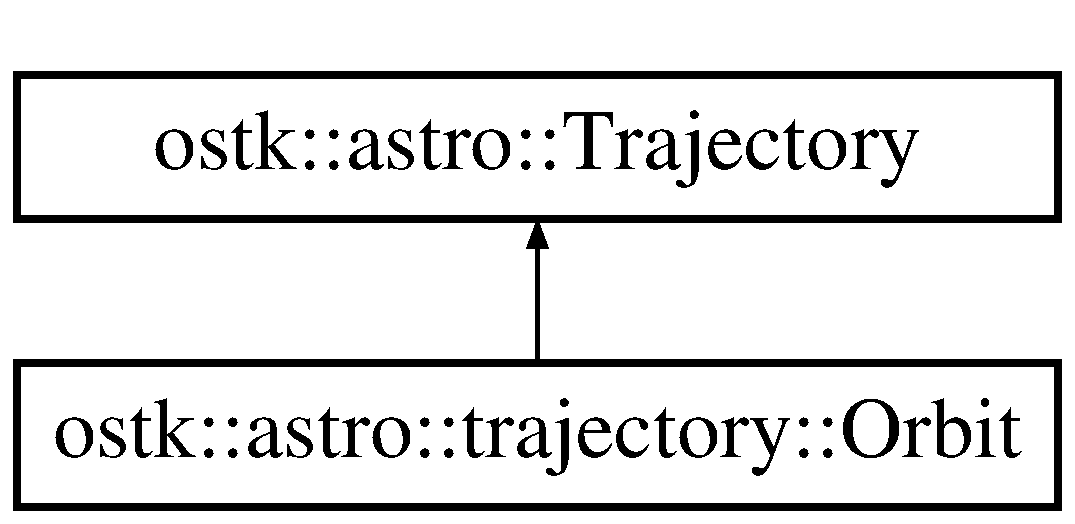
\includegraphics[height=2.000000cm]{classostk_1_1astro_1_1trajectory_1_1_orbit}
\end{center}
\end{figure}
\doxysubsection*{Public Types}
\begin{DoxyCompactItemize}
\item 
enum \mbox{\hyperlink{classostk_1_1astro_1_1trajectory_1_1_orbit_a1cc449ad56374471a8ab4300dde979e7}{Frame\+Type}} \{ \newline
\mbox{\hyperlink{classostk_1_1astro_1_1trajectory_1_1_orbit_a1cc449ad56374471a8ab4300dde979e7aec0fc0100c4fc1ce4eea230c3dc10360}{Frame\+Type\+::\+Undefined}}, 
\mbox{\hyperlink{classostk_1_1astro_1_1trajectory_1_1_orbit_a1cc449ad56374471a8ab4300dde979e7acd3459b28418fa8fa75ffaba4f3e7c74}{Frame\+Type\+::\+N\+ED}}, 
\mbox{\hyperlink{classostk_1_1astro_1_1trajectory_1_1_orbit_a1cc449ad56374471a8ab4300dde979e7acdfe4a5ed313c123b78c17d455cfa94f}{Frame\+Type\+::\+L\+V\+LH}}, 
\mbox{\hyperlink{classostk_1_1astro_1_1trajectory_1_1_orbit_a1cc449ad56374471a8ab4300dde979e7ae01a717c5a8a11cf57f7fdcb96aedc9c}{Frame\+Type\+::\+V\+V\+LH}}, 
\newline
\mbox{\hyperlink{classostk_1_1astro_1_1trajectory_1_1_orbit_a1cc449ad56374471a8ab4300dde979e7a9f24a174bf2de776f4f87caef847746f}{Frame\+Type\+::\+L\+V\+L\+H\+GD}}, 
\mbox{\hyperlink{classostk_1_1astro_1_1trajectory_1_1_orbit_a1cc449ad56374471a8ab4300dde979e7a4f190ed692b3a94eb49da59c497c7f55}{Frame\+Type\+::\+Q\+SW}}, 
\mbox{\hyperlink{classostk_1_1astro_1_1trajectory_1_1_orbit_a1cc449ad56374471a8ab4300dde979e7a6d951949ba8af28fa54a8629ec0f8f17}{Frame\+Type\+::\+T\+NW}}, 
\mbox{\hyperlink{classostk_1_1astro_1_1trajectory_1_1_orbit_a1cc449ad56374471a8ab4300dde979e7ac6a33911cc53df9bdb84aac8d86a0565}{Frame\+Type\+::\+V\+NC}}
 \}
\item 
typedef Array$<$ \mbox{\hyperlink{classostk_1_1astro_1_1trajectory_1_1orbit_1_1_pass}{Pass}} $>$\+::Const\+Iterator \mbox{\hyperlink{classostk_1_1astro_1_1trajectory_1_1_orbit_a0873dc63f4453eb2c07447e2774e944f}{Const\+Pass\+Iterator}}
\end{DoxyCompactItemize}
\doxysubsection*{Public Member Functions}
\begin{DoxyCompactItemize}
\item 
\mbox{\hyperlink{classostk_1_1astro_1_1trajectory_1_1_orbit_aaccbf7c99f454ba6acd8aff68a2137bf}{Orbit}} (const \mbox{\hyperlink{classostk_1_1astro_1_1trajectory_1_1orbit_1_1_model}{orbit\+::\+Model}} \&a\+Model, const Shared$<$ const Celestial $>$ \&a\+Celestial\+Object\+S\+Ptr)
\item 
\mbox{\hyperlink{classostk_1_1astro_1_1trajectory_1_1_orbit_ac5396ec3866ad7afe7384bbfc4d41339}{Orbit}} (const Array$<$ \mbox{\hyperlink{classostk_1_1astro_1_1trajectory_1_1_state}{State}} $>$ \&a\+State\+Array, const Integer \&an\+Initial\+Revolution\+Number, const Shared$<$ const Celestial $>$ \&a\+Celestial\+Object\+S\+Ptr)
\item 
\mbox{\hyperlink{classostk_1_1astro_1_1trajectory_1_1_orbit_ac44603858b8379e0f2ded4236855c162}{Orbit}} (const \mbox{\hyperlink{classostk_1_1astro_1_1trajectory_1_1_orbit}{Orbit}} \&an\+Orbit)
\item 
\mbox{\hyperlink{classostk_1_1astro_1_1trajectory_1_1_orbit_aad56a0293156188474bcf1b78e55e249}{$\sim$\+Orbit}} ()
\item 
\mbox{\hyperlink{classostk_1_1astro_1_1trajectory_1_1_orbit}{Orbit}} \& \mbox{\hyperlink{classostk_1_1astro_1_1trajectory_1_1_orbit_a069e013323a8fa6c513ef07e1a26db73}{operator=}} (const \mbox{\hyperlink{classostk_1_1astro_1_1trajectory_1_1_orbit}{Orbit}} \&an\+Orbit)
\item 
bool \mbox{\hyperlink{classostk_1_1astro_1_1trajectory_1_1_orbit_aa3fdab43c081059d268984dca953cb7d}{operator==}} (const \mbox{\hyperlink{classostk_1_1astro_1_1trajectory_1_1_orbit}{Orbit}} \&an\+Orbit) const
\item 
bool \mbox{\hyperlink{classostk_1_1astro_1_1trajectory_1_1_orbit_a9c376b2163bc4fcca62abccaf03014d2}{operator!=}} (const \mbox{\hyperlink{classostk_1_1astro_1_1trajectory_1_1_orbit}{Orbit}} \&an\+Orbit) const
\item 
bool \mbox{\hyperlink{classostk_1_1astro_1_1trajectory_1_1_orbit_abb1c3d611881104558aa93c9eb948455}{is\+Defined}} () const
\item 
Integer \mbox{\hyperlink{classostk_1_1astro_1_1trajectory_1_1_orbit_aa8ca190bd7b20f4654e0338660f57907}{get\+Revolution\+Number\+At}} (const Instant \&an\+Instant) const
\item 
\mbox{\hyperlink{classostk_1_1astro_1_1trajectory_1_1orbit_1_1_pass}{Pass}} \mbox{\hyperlink{classostk_1_1astro_1_1trajectory_1_1_orbit_a6cf47ea28cb2fb72a2659284a997b3b5}{get\+Pass\+At}} (const Instant \&an\+Instant) const
\item 
\mbox{\hyperlink{classostk_1_1astro_1_1trajectory_1_1orbit_1_1_pass}{Pass}} \mbox{\hyperlink{classostk_1_1astro_1_1trajectory_1_1_orbit_adee37553d5e3a67ab23f749c9147dd5c}{get\+Pass\+With\+Revolution\+Number}} (const Integer \&a\+Revolution\+Number) const
\item 
Shared$<$ const Frame $>$ \mbox{\hyperlink{classostk_1_1astro_1_1trajectory_1_1_orbit_a2549ae1a3ce8be76f441cfa85e9ab5ee}{get\+Orbital\+Frame}} (const \mbox{\hyperlink{classostk_1_1astro_1_1trajectory_1_1_orbit_a1cc449ad56374471a8ab4300dde979e7}{Orbit\+::\+Frame\+Type}} \&a\+Frame\+Type) const
\item 
virtual void \mbox{\hyperlink{classostk_1_1astro_1_1trajectory_1_1_orbit_ae890e832785f84c3f03c1e103f952826}{print}} (std\+::ostream \&an\+Output\+Stream, bool display\+Decorator=true) const override
\begin{DoxyCompactList}\small\item\em Print trajectory to output stream. \end{DoxyCompactList}\end{DoxyCompactItemize}
\doxysubsection*{Static Public Member Functions}
\begin{DoxyCompactItemize}
\item 
static \mbox{\hyperlink{classostk_1_1astro_1_1trajectory_1_1_orbit}{Orbit}} \mbox{\hyperlink{classostk_1_1astro_1_1trajectory_1_1_orbit_a2b1bc936b69b8c70cd33a6b26c943f31}{Undefined}} ()
\begin{DoxyCompactList}\small\item\em Constructs an undefined orbit. \end{DoxyCompactList}\item 
static \mbox{\hyperlink{classostk_1_1astro_1_1trajectory_1_1_orbit}{Orbit}} \mbox{\hyperlink{classostk_1_1astro_1_1trajectory_1_1_orbit_aaf9d4274b72e4eb756212f7946edc237}{Circular}} (const Instant \&an\+Epoch, const Length \&an\+Altitude, const Angle \&an\+Inclination, const Shared$<$ const Celestial $>$ \&a\+Celestial\+Object\+S\+Ptr)
\begin{DoxyCompactList}\small\item\em Constructs a circular orbit. \end{DoxyCompactList}\item 
static \mbox{\hyperlink{classostk_1_1astro_1_1trajectory_1_1_orbit}{Orbit}} \mbox{\hyperlink{classostk_1_1astro_1_1trajectory_1_1_orbit_a88a5db265588461a9e756fd2aa4d3e4c}{Equatorial}} (const Instant \&an\+Epoch, const Length \&an\+Apoapsis\+Altitude, const Length \&a\+Periapsis\+Altitude, const Shared$<$ const Celestial $>$ \&a\+Celestial\+Object\+S\+Ptr)
\begin{DoxyCompactList}\small\item\em Constructs an equatorial orbit. \end{DoxyCompactList}\item 
static \mbox{\hyperlink{classostk_1_1astro_1_1trajectory_1_1_orbit}{Orbit}} \mbox{\hyperlink{classostk_1_1astro_1_1trajectory_1_1_orbit_a8070657a625af4dae7b79a23e5026dcd}{Circular\+Equatorial}} (const Instant \&an\+Epoch, const Length \&an\+Altitude, const Shared$<$ const Celestial $>$ \&a\+Celestial\+Object\+S\+Ptr)
\begin{DoxyCompactList}\small\item\em Constructs a circular-\/equatorial orbit. \end{DoxyCompactList}\item 
static \mbox{\hyperlink{classostk_1_1astro_1_1trajectory_1_1_orbit}{Orbit}} \mbox{\hyperlink{classostk_1_1astro_1_1trajectory_1_1_orbit_a24492769b1948a354dab07958a0f134c}{Geo\+Synchronous}} (const Instant \&an\+Epoch, const Angle \&an\+Inclination, const Angle \&a\+Longitude, const Shared$<$ const Celestial $>$ \&a\+Celestial\+Object\+S\+Ptr)
\begin{DoxyCompactList}\small\item\em Constructs a geosynchronous orbit. \end{DoxyCompactList}\item 
static \mbox{\hyperlink{classostk_1_1astro_1_1trajectory_1_1_orbit}{Orbit}} \mbox{\hyperlink{classostk_1_1astro_1_1trajectory_1_1_orbit_abd4a56f774275d0555d1d66a8ffc03dd}{Sun\+Synchronous}} (const Instant \&an\+Epoch, const Length \&an\+Altitude, const Time \&a\+Local\+Time\+At\+Descending\+Node, const Shared$<$ const Celestial $>$ \&a\+Celestial\+Object\+S\+Ptr, const Angle \&an\+Argument\+Of\+Latitude=Angle\+::\+Zero())
\begin{DoxyCompactList}\small\item\em Constructs a Sun-\/synchronous orbit. \end{DoxyCompactList}\item 
static String \mbox{\hyperlink{classostk_1_1astro_1_1trajectory_1_1_orbit_a329934037eb9eb4cacfcb2a5774753ed}{String\+From\+Frame\+Type}} (const \mbox{\hyperlink{classostk_1_1astro_1_1trajectory_1_1_orbit_a1cc449ad56374471a8ab4300dde979e7}{Orbit\+::\+Frame\+Type}} \&a\+Frame\+Type)
\end{DoxyCompactItemize}


\doxysubsection{Detailed Description}
Gravitationally curved trajectory of an object. 

\href{https://en.wikipedia.org/wiki/Orbit}{\texttt{ https\+://en.\+wikipedia.\+org/wiki/\+Orbit}} 

\doxysubsection{Member Typedef Documentation}
\mbox{\Hypertarget{classostk_1_1astro_1_1trajectory_1_1_orbit_a0873dc63f4453eb2c07447e2774e944f}\label{classostk_1_1astro_1_1trajectory_1_1_orbit_a0873dc63f4453eb2c07447e2774e944f}} 
\index{ostk::astro::trajectory::Orbit@{ostk::astro::trajectory::Orbit}!ConstPassIterator@{ConstPassIterator}}
\index{ConstPassIterator@{ConstPassIterator}!ostk::astro::trajectory::Orbit@{ostk::astro::trajectory::Orbit}}
\doxysubsubsection{\texorpdfstring{ConstPassIterator}{ConstPassIterator}}
{\footnotesize\ttfamily typedef Array$<$\mbox{\hyperlink{classostk_1_1astro_1_1trajectory_1_1orbit_1_1_pass}{Pass}}$>$\+::Const\+Iterator \mbox{\hyperlink{classostk_1_1astro_1_1trajectory_1_1_orbit_a0873dc63f4453eb2c07447e2774e944f}{ostk\+::astro\+::trajectory\+::\+Orbit\+::\+Const\+Pass\+Iterator}}}



\doxysubsection{Member Enumeration Documentation}
\mbox{\Hypertarget{classostk_1_1astro_1_1trajectory_1_1_orbit_a1cc449ad56374471a8ab4300dde979e7}\label{classostk_1_1astro_1_1trajectory_1_1_orbit_a1cc449ad56374471a8ab4300dde979e7}} 
\index{ostk::astro::trajectory::Orbit@{ostk::astro::trajectory::Orbit}!FrameType@{FrameType}}
\index{FrameType@{FrameType}!ostk::astro::trajectory::Orbit@{ostk::astro::trajectory::Orbit}}
\doxysubsubsection{\texorpdfstring{FrameType}{FrameType}}
{\footnotesize\ttfamily enum \mbox{\hyperlink{classostk_1_1astro_1_1trajectory_1_1_orbit_a1cc449ad56374471a8ab4300dde979e7}{ostk\+::astro\+::trajectory\+::\+Orbit\+::\+Frame\+Type}}\hspace{0.3cm}{\ttfamily [strong]}}

\begin{DoxyEnumFields}{Enumerator}
\raisebox{\heightof{T}}[0pt][0pt]{\index{Undefined@{Undefined}!ostk::astro::trajectory::Orbit@{ostk::astro::trajectory::Orbit}}\index{ostk::astro::trajectory::Orbit@{ostk::astro::trajectory::Orbit}!Undefined@{Undefined}}}\mbox{\Hypertarget{classostk_1_1astro_1_1trajectory_1_1_orbit_a1cc449ad56374471a8ab4300dde979e7aec0fc0100c4fc1ce4eea230c3dc10360}\label{classostk_1_1astro_1_1trajectory_1_1_orbit_a1cc449ad56374471a8ab4300dde979e7aec0fc0100c4fc1ce4eea230c3dc10360}} 
Undefined&Undefined frame. \\
\hline

\raisebox{\heightof{T}}[0pt][0pt]{\index{NED@{NED}!ostk::astro::trajectory::Orbit@{ostk::astro::trajectory::Orbit}}\index{ostk::astro::trajectory::Orbit@{ostk::astro::trajectory::Orbit}!NED@{NED}}}\mbox{\Hypertarget{classostk_1_1astro_1_1trajectory_1_1_orbit_a1cc449ad56374471a8ab4300dde979e7acd3459b28418fa8fa75ffaba4f3e7c74}\label{classostk_1_1astro_1_1trajectory_1_1_orbit_a1cc449ad56374471a8ab4300dde979e7acd3459b28418fa8fa75ffaba4f3e7c74}} 
N\+ED&North-\/\+East-\/\+Down (N\+ED) frame. \\
\hline

\raisebox{\heightof{T}}[0pt][0pt]{\index{LVLH@{LVLH}!ostk::astro::trajectory::Orbit@{ostk::astro::trajectory::Orbit}}\index{ostk::astro::trajectory::Orbit@{ostk::astro::trajectory::Orbit}!LVLH@{LVLH}}}\mbox{\Hypertarget{classostk_1_1astro_1_1trajectory_1_1_orbit_a1cc449ad56374471a8ab4300dde979e7acdfe4a5ed313c123b78c17d455cfa94f}\label{classostk_1_1astro_1_1trajectory_1_1_orbit_a1cc449ad56374471a8ab4300dde979e7acdfe4a5ed313c123b78c17d455cfa94f}} 
L\+V\+LH&Local Vertical, Local Horizontal (L\+V\+LH) frame (X axis aligned with position, Z axis aligned with orbital momentum) \\
\hline

\raisebox{\heightof{T}}[0pt][0pt]{\index{VVLH@{VVLH}!ostk::astro::trajectory::Orbit@{ostk::astro::trajectory::Orbit}}\index{ostk::astro::trajectory::Orbit@{ostk::astro::trajectory::Orbit}!VVLH@{VVLH}}}\mbox{\Hypertarget{classostk_1_1astro_1_1trajectory_1_1_orbit_a1cc449ad56374471a8ab4300dde979e7ae01a717c5a8a11cf57f7fdcb96aedc9c}\label{classostk_1_1astro_1_1trajectory_1_1_orbit_a1cc449ad56374471a8ab4300dde979e7ae01a717c5a8a11cf57f7fdcb96aedc9c}} 
V\+V\+LH&Vehicle Velocity, Local Horizontal (V\+V\+LH) frame (Z axis aligned with opposite of position, Y axis aligned with opposite of orbital momentum) \\
\hline

\raisebox{\heightof{T}}[0pt][0pt]{\index{LVLHGD@{LVLHGD}!ostk::astro::trajectory::Orbit@{ostk::astro::trajectory::Orbit}}\index{ostk::astro::trajectory::Orbit@{ostk::astro::trajectory::Orbit}!LVLHGD@{LVLHGD}}}\mbox{\Hypertarget{classostk_1_1astro_1_1trajectory_1_1_orbit_a1cc449ad56374471a8ab4300dde979e7a9f24a174bf2de776f4f87caef847746f}\label{classostk_1_1astro_1_1trajectory_1_1_orbit_a1cc449ad56374471a8ab4300dde979e7a9f24a174bf2de776f4f87caef847746f}} 
L\+V\+L\+H\+GD&Local Vertical, Local Horizontal Geo\+Detic (L\+V\+L\+H\+GD) frame. \\
\hline

\raisebox{\heightof{T}}[0pt][0pt]{\index{QSW@{QSW}!ostk::astro::trajectory::Orbit@{ostk::astro::trajectory::Orbit}}\index{ostk::astro::trajectory::Orbit@{ostk::astro::trajectory::Orbit}!QSW@{QSW}}}\mbox{\Hypertarget{classostk_1_1astro_1_1trajectory_1_1_orbit_a1cc449ad56374471a8ab4300dde979e7a4f190ed692b3a94eb49da59c497c7f55}\label{classostk_1_1astro_1_1trajectory_1_1_orbit_a1cc449ad56374471a8ab4300dde979e7a4f190ed692b3a94eb49da59c497c7f55}} 
Q\+SW&Q\+SW frame (X axis aligned with position, Z axis aligned with orbital momentum) \\
\hline

\raisebox{\heightof{T}}[0pt][0pt]{\index{TNW@{TNW}!ostk::astro::trajectory::Orbit@{ostk::astro::trajectory::Orbit}}\index{ostk::astro::trajectory::Orbit@{ostk::astro::trajectory::Orbit}!TNW@{TNW}}}\mbox{\Hypertarget{classostk_1_1astro_1_1trajectory_1_1_orbit_a1cc449ad56374471a8ab4300dde979e7a6d951949ba8af28fa54a8629ec0f8f17}\label{classostk_1_1astro_1_1trajectory_1_1_orbit_a1cc449ad56374471a8ab4300dde979e7a6d951949ba8af28fa54a8629ec0f8f17}} 
T\+NW&T\+NW frame (X axis aligned with velocity, Z axis aligned with orbital momentum) \\
\hline

\raisebox{\heightof{T}}[0pt][0pt]{\index{VNC@{VNC}!ostk::astro::trajectory::Orbit@{ostk::astro::trajectory::Orbit}}\index{ostk::astro::trajectory::Orbit@{ostk::astro::trajectory::Orbit}!VNC@{VNC}}}\mbox{\Hypertarget{classostk_1_1astro_1_1trajectory_1_1_orbit_a1cc449ad56374471a8ab4300dde979e7ac6a33911cc53df9bdb84aac8d86a0565}\label{classostk_1_1astro_1_1trajectory_1_1_orbit_a1cc449ad56374471a8ab4300dde979e7ac6a33911cc53df9bdb84aac8d86a0565}} 
V\+NC&Velocity -\/ Normal -\/ Co-\/normal (V\+NC) frame (X axis aligned with velocity, Y axis aligned with orbital momentum) \\
\hline

\end{DoxyEnumFields}


\doxysubsection{Constructor \& Destructor Documentation}
\mbox{\Hypertarget{classostk_1_1astro_1_1trajectory_1_1_orbit_aaccbf7c99f454ba6acd8aff68a2137bf}\label{classostk_1_1astro_1_1trajectory_1_1_orbit_aaccbf7c99f454ba6acd8aff68a2137bf}} 
\index{ostk::astro::trajectory::Orbit@{ostk::astro::trajectory::Orbit}!Orbit@{Orbit}}
\index{Orbit@{Orbit}!ostk::astro::trajectory::Orbit@{ostk::astro::trajectory::Orbit}}
\doxysubsubsection{\texorpdfstring{Orbit()}{Orbit()}\hspace{0.1cm}{\footnotesize\ttfamily [1/3]}}
{\footnotesize\ttfamily ostk\+::astro\+::trajectory\+::\+Orbit\+::\+Orbit (\begin{DoxyParamCaption}\item[{const \mbox{\hyperlink{classostk_1_1astro_1_1trajectory_1_1orbit_1_1_model}{orbit\+::\+Model}} \&}]{a\+Model,  }\item[{const Shared$<$ const Celestial $>$ \&}]{a\+Celestial\+Object\+S\+Ptr }\end{DoxyParamCaption})}

\mbox{\Hypertarget{classostk_1_1astro_1_1trajectory_1_1_orbit_ac5396ec3866ad7afe7384bbfc4d41339}\label{classostk_1_1astro_1_1trajectory_1_1_orbit_ac5396ec3866ad7afe7384bbfc4d41339}} 
\index{ostk::astro::trajectory::Orbit@{ostk::astro::trajectory::Orbit}!Orbit@{Orbit}}
\index{Orbit@{Orbit}!ostk::astro::trajectory::Orbit@{ostk::astro::trajectory::Orbit}}
\doxysubsubsection{\texorpdfstring{Orbit()}{Orbit()}\hspace{0.1cm}{\footnotesize\ttfamily [2/3]}}
{\footnotesize\ttfamily ostk\+::astro\+::trajectory\+::\+Orbit\+::\+Orbit (\begin{DoxyParamCaption}\item[{const Array$<$ \mbox{\hyperlink{classostk_1_1astro_1_1trajectory_1_1_state}{State}} $>$ \&}]{a\+State\+Array,  }\item[{const Integer \&}]{an\+Initial\+Revolution\+Number,  }\item[{const Shared$<$ const Celestial $>$ \&}]{a\+Celestial\+Object\+S\+Ptr }\end{DoxyParamCaption})}

\mbox{\Hypertarget{classostk_1_1astro_1_1trajectory_1_1_orbit_ac44603858b8379e0f2ded4236855c162}\label{classostk_1_1astro_1_1trajectory_1_1_orbit_ac44603858b8379e0f2ded4236855c162}} 
\index{ostk::astro::trajectory::Orbit@{ostk::astro::trajectory::Orbit}!Orbit@{Orbit}}
\index{Orbit@{Orbit}!ostk::astro::trajectory::Orbit@{ostk::astro::trajectory::Orbit}}
\doxysubsubsection{\texorpdfstring{Orbit()}{Orbit()}\hspace{0.1cm}{\footnotesize\ttfamily [3/3]}}
{\footnotesize\ttfamily ostk\+::astro\+::trajectory\+::\+Orbit\+::\+Orbit (\begin{DoxyParamCaption}\item[{const \mbox{\hyperlink{classostk_1_1astro_1_1trajectory_1_1_orbit}{Orbit}} \&}]{an\+Orbit }\end{DoxyParamCaption})}

\mbox{\Hypertarget{classostk_1_1astro_1_1trajectory_1_1_orbit_aad56a0293156188474bcf1b78e55e249}\label{classostk_1_1astro_1_1trajectory_1_1_orbit_aad56a0293156188474bcf1b78e55e249}} 
\index{ostk::astro::trajectory::Orbit@{ostk::astro::trajectory::Orbit}!````~Orbit@{$\sim$Orbit}}
\index{````~Orbit@{$\sim$Orbit}!ostk::astro::trajectory::Orbit@{ostk::astro::trajectory::Orbit}}
\doxysubsubsection{\texorpdfstring{$\sim$Orbit()}{~Orbit()}}
{\footnotesize\ttfamily ostk\+::astro\+::trajectory\+::\+Orbit\+::$\sim$\+Orbit (\begin{DoxyParamCaption}{ }\end{DoxyParamCaption})}



\doxysubsection{Member Function Documentation}
\mbox{\Hypertarget{classostk_1_1astro_1_1trajectory_1_1_orbit_aaf9d4274b72e4eb756212f7946edc237}\label{classostk_1_1astro_1_1trajectory_1_1_orbit_aaf9d4274b72e4eb756212f7946edc237}} 
\index{ostk::astro::trajectory::Orbit@{ostk::astro::trajectory::Orbit}!Circular@{Circular}}
\index{Circular@{Circular}!ostk::astro::trajectory::Orbit@{ostk::astro::trajectory::Orbit}}
\doxysubsubsection{\texorpdfstring{Circular()}{Circular()}}
{\footnotesize\ttfamily \mbox{\hyperlink{classostk_1_1astro_1_1trajectory_1_1_orbit}{Orbit}} ostk\+::astro\+::trajectory\+::\+Orbit\+::\+Circular (\begin{DoxyParamCaption}\item[{const Instant \&}]{an\+Epoch,  }\item[{const Length \&}]{an\+Altitude,  }\item[{const Angle \&}]{an\+Inclination,  }\item[{const Shared$<$ const Celestial $>$ \&}]{a\+Celestial\+Object\+S\+Ptr }\end{DoxyParamCaption})\hspace{0.3cm}{\ttfamily [static]}}



Constructs a circular orbit. 

\begin{DoxyVerb}         Model: Kepler (No Perturbation).
\end{DoxyVerb}



\begin{DoxyParams}{Parameters}
{\em an\+Epoch} & An orbit epoch \\
\hline
{\em an\+Altitude} & An orbit altitude (wrt. equatorial radius) \\
\hline
{\em an\+Inclination} & An orbit inclination \\
\hline
{\em a\+Celestial\+Object\+S\+Ptr} & A shared pointer to a central celestial body \\
\hline
\end{DoxyParams}
\begin{DoxyReturn}{Returns}
Circular orbit 
\end{DoxyReturn}
\mbox{\Hypertarget{classostk_1_1astro_1_1trajectory_1_1_orbit_a8070657a625af4dae7b79a23e5026dcd}\label{classostk_1_1astro_1_1trajectory_1_1_orbit_a8070657a625af4dae7b79a23e5026dcd}} 
\index{ostk::astro::trajectory::Orbit@{ostk::astro::trajectory::Orbit}!CircularEquatorial@{CircularEquatorial}}
\index{CircularEquatorial@{CircularEquatorial}!ostk::astro::trajectory::Orbit@{ostk::astro::trajectory::Orbit}}
\doxysubsubsection{\texorpdfstring{CircularEquatorial()}{CircularEquatorial()}}
{\footnotesize\ttfamily \mbox{\hyperlink{classostk_1_1astro_1_1trajectory_1_1_orbit}{Orbit}} ostk\+::astro\+::trajectory\+::\+Orbit\+::\+Circular\+Equatorial (\begin{DoxyParamCaption}\item[{const Instant \&}]{an\+Epoch,  }\item[{const Length \&}]{an\+Altitude,  }\item[{const Shared$<$ const Celestial $>$ \&}]{a\+Celestial\+Object\+S\+Ptr }\end{DoxyParamCaption})\hspace{0.3cm}{\ttfamily [static]}}



Constructs a circular-\/equatorial orbit. 

\begin{DoxyVerb}         Model: Kepler (No Perturbation).
\end{DoxyVerb}



\begin{DoxyParams}{Parameters}
{\em an\+Epoch} & An orbit epoch \\
\hline
{\em an\+Altitude} & An orbit altitude (wrt. equatorial radius) \\
\hline
{\em a\+Celestial\+Object\+S\+Ptr} & A shared pointer to a central celestial body \\
\hline
\end{DoxyParams}
\begin{DoxyReturn}{Returns}
Circular-\/equatorial orbit 
\end{DoxyReturn}
\mbox{\Hypertarget{classostk_1_1astro_1_1trajectory_1_1_orbit_a88a5db265588461a9e756fd2aa4d3e4c}\label{classostk_1_1astro_1_1trajectory_1_1_orbit_a88a5db265588461a9e756fd2aa4d3e4c}} 
\index{ostk::astro::trajectory::Orbit@{ostk::astro::trajectory::Orbit}!Equatorial@{Equatorial}}
\index{Equatorial@{Equatorial}!ostk::astro::trajectory::Orbit@{ostk::astro::trajectory::Orbit}}
\doxysubsubsection{\texorpdfstring{Equatorial()}{Equatorial()}}
{\footnotesize\ttfamily \mbox{\hyperlink{classostk_1_1astro_1_1trajectory_1_1_orbit}{Orbit}} ostk\+::astro\+::trajectory\+::\+Orbit\+::\+Equatorial (\begin{DoxyParamCaption}\item[{const Instant \&}]{an\+Epoch,  }\item[{const Length \&}]{an\+Apoapsis\+Altitude,  }\item[{const Length \&}]{a\+Periapsis\+Altitude,  }\item[{const Shared$<$ const Celestial $>$ \&}]{a\+Celestial\+Object\+S\+Ptr }\end{DoxyParamCaption})\hspace{0.3cm}{\ttfamily [static]}}



Constructs an equatorial orbit. 

\begin{DoxyVerb}         Model: Kepler (No Perturbation).
\end{DoxyVerb}



\begin{DoxyParams}{Parameters}
{\em an\+Epoch} & An orbit epoch \\
\hline
{\em an\+Apoapsis\+Altitude} & An orbit apoapsis altitude (wrt. equatorial radius) \\
\hline
{\em a\+Periapsis\+Altitude} & An orbit periapsis altitude (wrt. equatorial radius) \\
\hline
{\em a\+Celestial\+Object\+S\+Ptr} & A shared pointer to a central celestial body \\
\hline
\end{DoxyParams}
\begin{DoxyReturn}{Returns}
Equatorial orbit 
\end{DoxyReturn}
\mbox{\Hypertarget{classostk_1_1astro_1_1trajectory_1_1_orbit_a24492769b1948a354dab07958a0f134c}\label{classostk_1_1astro_1_1trajectory_1_1_orbit_a24492769b1948a354dab07958a0f134c}} 
\index{ostk::astro::trajectory::Orbit@{ostk::astro::trajectory::Orbit}!GeoSynchronous@{GeoSynchronous}}
\index{GeoSynchronous@{GeoSynchronous}!ostk::astro::trajectory::Orbit@{ostk::astro::trajectory::Orbit}}
\doxysubsubsection{\texorpdfstring{GeoSynchronous()}{GeoSynchronous()}}
{\footnotesize\ttfamily \mbox{\hyperlink{classostk_1_1astro_1_1trajectory_1_1_orbit}{Orbit}} ostk\+::astro\+::trajectory\+::\+Orbit\+::\+Geo\+Synchronous (\begin{DoxyParamCaption}\item[{const Instant \&}]{an\+Epoch,  }\item[{const Angle \&}]{an\+Inclination,  }\item[{const Angle \&}]{a\+Longitude,  }\item[{const Shared$<$ const Celestial $>$ \&}]{a\+Celestial\+Object\+S\+Ptr }\end{DoxyParamCaption})\hspace{0.3cm}{\ttfamily [static]}}



Constructs a geosynchronous orbit. 

\begin{DoxyVerb}         Model: Kepler (J2 Perturbation).
\end{DoxyVerb}



\begin{DoxyParams}{Parameters}
{\em an\+Epoch} & An orbit epoch \\
\hline
{\em an\+Inclination} & An orbit inclination \\
\hline
{\em a\+Longitude} & A longitude above the surface \\
\hline
{\em a\+Celestial\+Object\+S\+Ptr} & A shared pointer to a central celestial body \\
\hline
\end{DoxyParams}
\begin{DoxyReturn}{Returns}
Circular orbit 
\end{DoxyReturn}
\mbox{\Hypertarget{classostk_1_1astro_1_1trajectory_1_1_orbit_a2549ae1a3ce8be76f441cfa85e9ab5ee}\label{classostk_1_1astro_1_1trajectory_1_1_orbit_a2549ae1a3ce8be76f441cfa85e9ab5ee}} 
\index{ostk::astro::trajectory::Orbit@{ostk::astro::trajectory::Orbit}!getOrbitalFrame@{getOrbitalFrame}}
\index{getOrbitalFrame@{getOrbitalFrame}!ostk::astro::trajectory::Orbit@{ostk::astro::trajectory::Orbit}}
\doxysubsubsection{\texorpdfstring{getOrbitalFrame()}{getOrbitalFrame()}}
{\footnotesize\ttfamily Shared$<$ const Frame $>$ ostk\+::astro\+::trajectory\+::\+Orbit\+::get\+Orbital\+Frame (\begin{DoxyParamCaption}\item[{const \mbox{\hyperlink{classostk_1_1astro_1_1trajectory_1_1_orbit_a1cc449ad56374471a8ab4300dde979e7}{Orbit\+::\+Frame\+Type}} \&}]{a\+Frame\+Type }\end{DoxyParamCaption}) const}

\mbox{\Hypertarget{classostk_1_1astro_1_1trajectory_1_1_orbit_a6cf47ea28cb2fb72a2659284a997b3b5}\label{classostk_1_1astro_1_1trajectory_1_1_orbit_a6cf47ea28cb2fb72a2659284a997b3b5}} 
\index{ostk::astro::trajectory::Orbit@{ostk::astro::trajectory::Orbit}!getPassAt@{getPassAt}}
\index{getPassAt@{getPassAt}!ostk::astro::trajectory::Orbit@{ostk::astro::trajectory::Orbit}}
\doxysubsubsection{\texorpdfstring{getPassAt()}{getPassAt()}}
{\footnotesize\ttfamily \mbox{\hyperlink{classostk_1_1astro_1_1trajectory_1_1orbit_1_1_pass}{Pass}} ostk\+::astro\+::trajectory\+::\+Orbit\+::get\+Pass\+At (\begin{DoxyParamCaption}\item[{const Instant \&}]{an\+Instant }\end{DoxyParamCaption}) const}

\mbox{\Hypertarget{classostk_1_1astro_1_1trajectory_1_1_orbit_adee37553d5e3a67ab23f749c9147dd5c}\label{classostk_1_1astro_1_1trajectory_1_1_orbit_adee37553d5e3a67ab23f749c9147dd5c}} 
\index{ostk::astro::trajectory::Orbit@{ostk::astro::trajectory::Orbit}!getPassWithRevolutionNumber@{getPassWithRevolutionNumber}}
\index{getPassWithRevolutionNumber@{getPassWithRevolutionNumber}!ostk::astro::trajectory::Orbit@{ostk::astro::trajectory::Orbit}}
\doxysubsubsection{\texorpdfstring{getPassWithRevolutionNumber()}{getPassWithRevolutionNumber()}}
{\footnotesize\ttfamily \mbox{\hyperlink{classostk_1_1astro_1_1trajectory_1_1orbit_1_1_pass}{Pass}} ostk\+::astro\+::trajectory\+::\+Orbit\+::get\+Pass\+With\+Revolution\+Number (\begin{DoxyParamCaption}\item[{const Integer \&}]{a\+Revolution\+Number }\end{DoxyParamCaption}) const}

\mbox{\Hypertarget{classostk_1_1astro_1_1trajectory_1_1_orbit_aa8ca190bd7b20f4654e0338660f57907}\label{classostk_1_1astro_1_1trajectory_1_1_orbit_aa8ca190bd7b20f4654e0338660f57907}} 
\index{ostk::astro::trajectory::Orbit@{ostk::astro::trajectory::Orbit}!getRevolutionNumberAt@{getRevolutionNumberAt}}
\index{getRevolutionNumberAt@{getRevolutionNumberAt}!ostk::astro::trajectory::Orbit@{ostk::astro::trajectory::Orbit}}
\doxysubsubsection{\texorpdfstring{getRevolutionNumberAt()}{getRevolutionNumberAt()}}
{\footnotesize\ttfamily Integer ostk\+::astro\+::trajectory\+::\+Orbit\+::get\+Revolution\+Number\+At (\begin{DoxyParamCaption}\item[{const Instant \&}]{an\+Instant }\end{DoxyParamCaption}) const}

\mbox{\Hypertarget{classostk_1_1astro_1_1trajectory_1_1_orbit_abb1c3d611881104558aa93c9eb948455}\label{classostk_1_1astro_1_1trajectory_1_1_orbit_abb1c3d611881104558aa93c9eb948455}} 
\index{ostk::astro::trajectory::Orbit@{ostk::astro::trajectory::Orbit}!isDefined@{isDefined}}
\index{isDefined@{isDefined}!ostk::astro::trajectory::Orbit@{ostk::astro::trajectory::Orbit}}
\doxysubsubsection{\texorpdfstring{isDefined()}{isDefined()}}
{\footnotesize\ttfamily bool ostk\+::astro\+::trajectory\+::\+Orbit\+::is\+Defined (\begin{DoxyParamCaption}{ }\end{DoxyParamCaption}) const}

\mbox{\Hypertarget{classostk_1_1astro_1_1trajectory_1_1_orbit_a9c376b2163bc4fcca62abccaf03014d2}\label{classostk_1_1astro_1_1trajectory_1_1_orbit_a9c376b2163bc4fcca62abccaf03014d2}} 
\index{ostk::astro::trajectory::Orbit@{ostk::astro::trajectory::Orbit}!operator"!=@{operator"!=}}
\index{operator"!=@{operator"!=}!ostk::astro::trajectory::Orbit@{ostk::astro::trajectory::Orbit}}
\doxysubsubsection{\texorpdfstring{operator"!=()}{operator!=()}}
{\footnotesize\ttfamily bool ostk\+::astro\+::trajectory\+::\+Orbit\+::operator!= (\begin{DoxyParamCaption}\item[{const \mbox{\hyperlink{classostk_1_1astro_1_1trajectory_1_1_orbit}{Orbit}} \&}]{an\+Orbit }\end{DoxyParamCaption}) const}

\mbox{\Hypertarget{classostk_1_1astro_1_1trajectory_1_1_orbit_a069e013323a8fa6c513ef07e1a26db73}\label{classostk_1_1astro_1_1trajectory_1_1_orbit_a069e013323a8fa6c513ef07e1a26db73}} 
\index{ostk::astro::trajectory::Orbit@{ostk::astro::trajectory::Orbit}!operator=@{operator=}}
\index{operator=@{operator=}!ostk::astro::trajectory::Orbit@{ostk::astro::trajectory::Orbit}}
\doxysubsubsection{\texorpdfstring{operator=()}{operator=()}}
{\footnotesize\ttfamily \mbox{\hyperlink{classostk_1_1astro_1_1trajectory_1_1_orbit}{Orbit}} \& ostk\+::astro\+::trajectory\+::\+Orbit\+::operator= (\begin{DoxyParamCaption}\item[{const \mbox{\hyperlink{classostk_1_1astro_1_1trajectory_1_1_orbit}{Orbit}} \&}]{an\+Orbit }\end{DoxyParamCaption})}

\mbox{\Hypertarget{classostk_1_1astro_1_1trajectory_1_1_orbit_aa3fdab43c081059d268984dca953cb7d}\label{classostk_1_1astro_1_1trajectory_1_1_orbit_aa3fdab43c081059d268984dca953cb7d}} 
\index{ostk::astro::trajectory::Orbit@{ostk::astro::trajectory::Orbit}!operator==@{operator==}}
\index{operator==@{operator==}!ostk::astro::trajectory::Orbit@{ostk::astro::trajectory::Orbit}}
\doxysubsubsection{\texorpdfstring{operator==()}{operator==()}}
{\footnotesize\ttfamily bool ostk\+::astro\+::trajectory\+::\+Orbit\+::operator== (\begin{DoxyParamCaption}\item[{const \mbox{\hyperlink{classostk_1_1astro_1_1trajectory_1_1_orbit}{Orbit}} \&}]{an\+Orbit }\end{DoxyParamCaption}) const}

\mbox{\Hypertarget{classostk_1_1astro_1_1trajectory_1_1_orbit_ae890e832785f84c3f03c1e103f952826}\label{classostk_1_1astro_1_1trajectory_1_1_orbit_ae890e832785f84c3f03c1e103f952826}} 
\index{ostk::astro::trajectory::Orbit@{ostk::astro::trajectory::Orbit}!print@{print}}
\index{print@{print}!ostk::astro::trajectory::Orbit@{ostk::astro::trajectory::Orbit}}
\doxysubsubsection{\texorpdfstring{print()}{print()}}
{\footnotesize\ttfamily void ostk\+::astro\+::trajectory\+::\+Orbit\+::print (\begin{DoxyParamCaption}\item[{std\+::ostream \&}]{an\+Output\+Stream,  }\item[{bool}]{display\+Decorator = {\ttfamily true} }\end{DoxyParamCaption}) const\hspace{0.3cm}{\ttfamily [override]}, {\ttfamily [virtual]}}



Print trajectory to output stream. 


\begin{DoxyCode}{0}
\DoxyCodeLine{\mbox{\hyperlink{classostk_1_1astro_1_1_trajectory_a9333200bd6afed5aef4f5aad8a2a8e84}{Trajectory}} trajectory = \{ ... \} ;}
\DoxyCodeLine{trajectory.print(std::cout, \textcolor{keyword}{true}) ;}
\end{DoxyCode}



\begin{DoxyParams}{Parameters}
{\em an\+Output\+Stream} & An output stream \\
\hline
{\em display\+Decorator} & If true, display decorator \\
\hline
\end{DoxyParams}


Reimplemented from \mbox{\hyperlink{classostk_1_1astro_1_1_trajectory_aac11fb7c53f4cf970f52f681a75c5261}{ostk\+::astro\+::\+Trajectory}}.

\mbox{\Hypertarget{classostk_1_1astro_1_1trajectory_1_1_orbit_a329934037eb9eb4cacfcb2a5774753ed}\label{classostk_1_1astro_1_1trajectory_1_1_orbit_a329934037eb9eb4cacfcb2a5774753ed}} 
\index{ostk::astro::trajectory::Orbit@{ostk::astro::trajectory::Orbit}!StringFromFrameType@{StringFromFrameType}}
\index{StringFromFrameType@{StringFromFrameType}!ostk::astro::trajectory::Orbit@{ostk::astro::trajectory::Orbit}}
\doxysubsubsection{\texorpdfstring{StringFromFrameType()}{StringFromFrameType()}}
{\footnotesize\ttfamily String ostk\+::astro\+::trajectory\+::\+Orbit\+::\+String\+From\+Frame\+Type (\begin{DoxyParamCaption}\item[{const \mbox{\hyperlink{classostk_1_1astro_1_1trajectory_1_1_orbit_a1cc449ad56374471a8ab4300dde979e7}{Orbit\+::\+Frame\+Type}} \&}]{a\+Frame\+Type }\end{DoxyParamCaption})\hspace{0.3cm}{\ttfamily [static]}}

\mbox{\Hypertarget{classostk_1_1astro_1_1trajectory_1_1_orbit_abd4a56f774275d0555d1d66a8ffc03dd}\label{classostk_1_1astro_1_1trajectory_1_1_orbit_abd4a56f774275d0555d1d66a8ffc03dd}} 
\index{ostk::astro::trajectory::Orbit@{ostk::astro::trajectory::Orbit}!SunSynchronous@{SunSynchronous}}
\index{SunSynchronous@{SunSynchronous}!ostk::astro::trajectory::Orbit@{ostk::astro::trajectory::Orbit}}
\doxysubsubsection{\texorpdfstring{SunSynchronous()}{SunSynchronous()}}
{\footnotesize\ttfamily \mbox{\hyperlink{classostk_1_1astro_1_1trajectory_1_1_orbit}{Orbit}} ostk\+::astro\+::trajectory\+::\+Orbit\+::\+Sun\+Synchronous (\begin{DoxyParamCaption}\item[{const Instant \&}]{an\+Epoch,  }\item[{const Length \&}]{an\+Altitude,  }\item[{const Time \&}]{a\+Local\+Time\+At\+Descending\+Node,  }\item[{const Shared$<$ const Celestial $>$ \&}]{a\+Celestial\+Object\+S\+Ptr,  }\item[{const Angle \&}]{an\+Argument\+Of\+Latitude = {\ttfamily Angle\+:\+:Zero()} }\end{DoxyParamCaption})\hspace{0.3cm}{\ttfamily [static]}}



Constructs a Sun-\/synchronous orbit. 

\begin{DoxyVerb}         Model: Kepler (J2 Perturbation).
\end{DoxyVerb}



\begin{DoxyParams}{Parameters}
{\em an\+Epoch} & An orbit epoch \\
\hline
{\em an\+Altitude} & An orbit altitude (wrt. equatorial radius) \\
\hline
{\em a\+Local\+Time\+At\+Descending\+Node} & A local time at descending node \\
\hline
{\em a\+Celestial\+Object\+S\+Ptr} & A shared pointer to a central celestial body \\
\hline
{\em an\+Argument\+Of\+Latitude} & An argument of latitude \\
\hline
\end{DoxyParams}
\begin{DoxyReturn}{Returns}
Sun-\/synchronous orbit 
\end{DoxyReturn}
Capderou M., Handbook of Satellite Orbits\+: From Kepler to G\+PS, p.\+292\mbox{\Hypertarget{classostk_1_1astro_1_1trajectory_1_1_orbit_a2b1bc936b69b8c70cd33a6b26c943f31}\label{classostk_1_1astro_1_1trajectory_1_1_orbit_a2b1bc936b69b8c70cd33a6b26c943f31}} 
\index{ostk::astro::trajectory::Orbit@{ostk::astro::trajectory::Orbit}!Undefined@{Undefined}}
\index{Undefined@{Undefined}!ostk::astro::trajectory::Orbit@{ostk::astro::trajectory::Orbit}}
\doxysubsubsection{\texorpdfstring{Undefined()}{Undefined()}}
{\footnotesize\ttfamily \mbox{\hyperlink{classostk_1_1astro_1_1trajectory_1_1_orbit}{Orbit}} ostk\+::astro\+::trajectory\+::\+Orbit\+::\+Undefined (\begin{DoxyParamCaption}{ }\end{DoxyParamCaption})\hspace{0.3cm}{\ttfamily [static]}}



Constructs an undefined orbit. 

\begin{DoxyVerb}         Undefined orbit 
\end{DoxyVerb}
 

The documentation for this class was generated from the following files\+:\begin{DoxyCompactItemize}
\item 
include/\+Open\+Space\+Toolkit/\+Astrodynamics/\+Trajectory/\mbox{\hyperlink{_orbit_8hpp}{Orbit.\+hpp}}\item 
src/\+Open\+Space\+Toolkit/\+Astrodynamics/\+Trajectory/\mbox{\hyperlink{_orbit_8cpp}{Orbit.\+cpp}}\end{DoxyCompactItemize}

\hypertarget{classostk_1_1astro_1_1trajectory_1_1orbit_1_1_pass}{}\doxysection{ostk\+::astro\+::trajectory\+::orbit\+::Pass Class Reference}
\label{classostk_1_1astro_1_1trajectory_1_1orbit_1_1_pass}\index{ostk::astro::trajectory::orbit::Pass@{ostk::astro::trajectory::orbit::Pass}}


A revolution of an orbiting object.  




{\ttfamily \#include $<$Pass.\+hpp$>$}

\doxysubsection*{Public Types}
\begin{DoxyCompactItemize}
\item 
enum \mbox{\hyperlink{classostk_1_1astro_1_1trajectory_1_1orbit_1_1_pass_a74449dbd104c6a24462b373cc55febcc}{Type}} \{ \mbox{\hyperlink{classostk_1_1astro_1_1trajectory_1_1orbit_1_1_pass_a74449dbd104c6a24462b373cc55febccaec0fc0100c4fc1ce4eea230c3dc10360}{Type\+::\+Undefined}}, 
\mbox{\hyperlink{classostk_1_1astro_1_1trajectory_1_1orbit_1_1_pass_a74449dbd104c6a24462b373cc55febccaae94f80b3ce82062a5dd7815daa04f9d}{Type\+::\+Complete}}, 
\mbox{\hyperlink{classostk_1_1astro_1_1trajectory_1_1orbit_1_1_pass_a74449dbd104c6a24462b373cc55febcca44ffd38a6dea695cbe2b34efdcc6cf27}{Type\+::\+Partial}}
 \}
\begin{DoxyCompactList}\small\item\em The type of the pass. \end{DoxyCompactList}\item 
enum \mbox{\hyperlink{classostk_1_1astro_1_1trajectory_1_1orbit_1_1_pass_a9fb48e13f29c899a8b74c43091fe4203}{Phase}} \{ \mbox{\hyperlink{classostk_1_1astro_1_1trajectory_1_1orbit_1_1_pass_a9fb48e13f29c899a8b74c43091fe4203aec0fc0100c4fc1ce4eea230c3dc10360}{Phase\+::\+Undefined}}, 
\mbox{\hyperlink{classostk_1_1astro_1_1trajectory_1_1orbit_1_1_pass_a9fb48e13f29c899a8b74c43091fe4203acf3fb1ff52ea1eed3347ac5401ee7f0c}{Phase\+::\+Ascending}}, 
\mbox{\hyperlink{classostk_1_1astro_1_1trajectory_1_1orbit_1_1_pass_a9fb48e13f29c899a8b74c43091fe4203ae3cf5ac19407b1a62c6fccaff675a53b}{Phase\+::\+Descending}}
 \}
\begin{DoxyCompactList}\small\item\em The phase of the pass. \end{DoxyCompactList}\end{DoxyCompactItemize}
\doxysubsection*{Public Member Functions}
\begin{DoxyCompactItemize}
\item 
\mbox{\hyperlink{classostk_1_1astro_1_1trajectory_1_1orbit_1_1_pass_a3e4072abac1191aa4b31e68e90cdd993}{Pass}} (const Integer \&a\+Revolution\+Number, const Instant \&an\+Instant\+At\+Ascending\+Node, const Instant \&an\+Instant\+At\+North\+Point, const Instant \&an\+Instant\+At\+Descending\+Node, const Instant \&an\+Instant\+At\+South\+Point, const Instant \&an\+Instant\+At\+Pass\+Break)
\begin{DoxyCompactList}\small\item\em Constructs a pass. \end{DoxyCompactList}\item 
bool \mbox{\hyperlink{classostk_1_1astro_1_1trajectory_1_1orbit_1_1_pass_ad2980a78e9a34cc95c906d72839450a0}{operator==}} (const \mbox{\hyperlink{classostk_1_1astro_1_1trajectory_1_1orbit_1_1_pass}{Pass}} \&a\+Pass) const
\begin{DoxyCompactList}\small\item\em Equality operator. \end{DoxyCompactList}\item 
bool \mbox{\hyperlink{classostk_1_1astro_1_1trajectory_1_1orbit_1_1_pass_ab5b73ab2c54e082774dc9cc16ad5097f}{operator!=}} (const \mbox{\hyperlink{classostk_1_1astro_1_1trajectory_1_1orbit_1_1_pass}{Pass}} \&a\+Pass) const
\begin{DoxyCompactList}\small\item\em Inequality operator. \end{DoxyCompactList}\item 
bool \mbox{\hyperlink{classostk_1_1astro_1_1trajectory_1_1orbit_1_1_pass_acaf286ca5433a63f9e6e7b226cde7b81}{is\+Defined}} () const
\begin{DoxyCompactList}\small\item\em Checks if the pass is defined. \end{DoxyCompactList}\item 
bool \mbox{\hyperlink{classostk_1_1astro_1_1trajectory_1_1orbit_1_1_pass_af25e2c67077dbe78999af64bae0a6f83}{is\+Complete}} () const
\begin{DoxyCompactList}\small\item\em Checks if the pass is complete. \end{DoxyCompactList}\item 
\mbox{\hyperlink{classostk_1_1astro_1_1trajectory_1_1orbit_1_1_pass_a74449dbd104c6a24462b373cc55febcc}{Pass\+::\+Type}} \mbox{\hyperlink{classostk_1_1astro_1_1trajectory_1_1orbit_1_1_pass_a059f8209971303cc8961a747e690258e}{get\+Type}} () const
\begin{DoxyCompactList}\small\item\em Gets the type of the pass. \end{DoxyCompactList}\item 
Integer \mbox{\hyperlink{classostk_1_1astro_1_1trajectory_1_1orbit_1_1_pass_abfc538f6a638420298886228f972855d}{get\+Revolution\+Number}} () const
\begin{DoxyCompactList}\small\item\em Gets the revolution number of the pass. \end{DoxyCompactList}\item 
Duration \mbox{\hyperlink{classostk_1_1astro_1_1trajectory_1_1orbit_1_1_pass_a24ae85ff9798ebcf03fd679aa97c1eb1}{get\+Duration}} () const
\begin{DoxyCompactList}\small\item\em Gets the duration of the pass. \end{DoxyCompactList}\item 
const Instant \& \mbox{\hyperlink{classostk_1_1astro_1_1trajectory_1_1orbit_1_1_pass_ac53192a54b8d5fac7175d7624fe37b33}{access\+Instant\+At\+Ascending\+Node}} () const
\begin{DoxyCompactList}\small\item\em Accesses the instant at the ascending node of the pass. \end{DoxyCompactList}\item 
const Instant \& \mbox{\hyperlink{classostk_1_1astro_1_1trajectory_1_1orbit_1_1_pass_a7ebe5ce7299bff0d0679df076542755c}{access\+Instant\+At\+North\+Point}} () const
\begin{DoxyCompactList}\small\item\em Accesses the instant at the north point of the pass. \end{DoxyCompactList}\item 
const Instant \& \mbox{\hyperlink{classostk_1_1astro_1_1trajectory_1_1orbit_1_1_pass_a2093761b6a4ad91b9795a962d575cac4}{access\+Instant\+At\+Descending\+Node}} () const
\begin{DoxyCompactList}\small\item\em Accesses the instant at the descending node of the pass. \end{DoxyCompactList}\item 
const Instant \& \mbox{\hyperlink{classostk_1_1astro_1_1trajectory_1_1orbit_1_1_pass_af927b5e6fc4ffa6e12627bdba2d18cb3}{access\+Instant\+At\+South\+Point}} () const
\begin{DoxyCompactList}\small\item\em Accesses the instant at the south point of the pass. \end{DoxyCompactList}\item 
const Instant \& \mbox{\hyperlink{classostk_1_1astro_1_1trajectory_1_1orbit_1_1_pass_a4e113507418add9255e21e74b6af7a77}{access\+Instant\+At\+Pass\+Break}} () const
\begin{DoxyCompactList}\small\item\em Accesses the instant at the break of the pass. \end{DoxyCompactList}\item 
void \mbox{\hyperlink{classostk_1_1astro_1_1trajectory_1_1orbit_1_1_pass_a137d76c79f749ed214c0bf4a3410f602}{print}} (std\+::ostream \&an\+Output\+Stream, bool display\+Decorator=true) const
\begin{DoxyCompactList}\small\item\em Print. \end{DoxyCompactList}\end{DoxyCompactItemize}
\doxysubsection*{Static Public Member Functions}
\begin{DoxyCompactItemize}
\item 
static \mbox{\hyperlink{classostk_1_1astro_1_1trajectory_1_1orbit_1_1_pass}{Pass}} \mbox{\hyperlink{classostk_1_1astro_1_1trajectory_1_1orbit_1_1_pass_ad1f97ee5361bce2ea9d3dd2211fa52bc}{Undefined}} ()
\begin{DoxyCompactList}\small\item\em Creates an undefined pass. \end{DoxyCompactList}\item 
static String \mbox{\hyperlink{classostk_1_1astro_1_1trajectory_1_1orbit_1_1_pass_ae3ba229e53fe1041c96a44c1609d3d28}{String\+From\+Type}} (const \mbox{\hyperlink{classostk_1_1astro_1_1trajectory_1_1orbit_1_1_pass_a74449dbd104c6a24462b373cc55febcc}{Pass\+::\+Type}} \&a\+Type)
\begin{DoxyCompactList}\small\item\em Converts a pass type to a string. \end{DoxyCompactList}\item 
static String \mbox{\hyperlink{classostk_1_1astro_1_1trajectory_1_1orbit_1_1_pass_aff910b1d0ea72c538ee087ff39cd62fa}{String\+From\+Phase}} (const \mbox{\hyperlink{classostk_1_1astro_1_1trajectory_1_1orbit_1_1_pass_a9fb48e13f29c899a8b74c43091fe4203}{Pass\+::\+Phase}} \&a\+Phase)
\begin{DoxyCompactList}\small\item\em Converts a pass phase to a string. \end{DoxyCompactList}\end{DoxyCompactItemize}
\doxysubsection*{Friends}
\begin{DoxyCompactItemize}
\item 
std\+::ostream \& \mbox{\hyperlink{classostk_1_1astro_1_1trajectory_1_1orbit_1_1_pass_a62c2257085205d3c714c5ca4350f84f4}{operator$<$$<$}} (std\+::ostream \&an\+Output\+Stream, const \mbox{\hyperlink{classostk_1_1astro_1_1trajectory_1_1orbit_1_1_pass}{Pass}} \&a\+Pass)
\begin{DoxyCompactList}\small\item\em Output stream operator. \end{DoxyCompactList}\end{DoxyCompactItemize}


\doxysubsection{Detailed Description}
A revolution of an orbiting object. 

This class represents a pass, which is a revolution of an orbiting object. It provides methods to get the type of the pass, the revolution number, and the instants at various points of the pass. \begin{DoxySeeAlso}{See also}
\href{http://help.agi.com/stk/11.3.0/index.htm\#vo/sat_pass.htm}{\texttt{ http\+://help.\+agi.\+com/stk/11.\+3.\+0/index.\+htm\#vo/sat\+\_\+pass.\+htm}} 
\end{DoxySeeAlso}


\doxysubsection{Member Enumeration Documentation}
\mbox{\Hypertarget{classostk_1_1astro_1_1trajectory_1_1orbit_1_1_pass_a9fb48e13f29c899a8b74c43091fe4203}\label{classostk_1_1astro_1_1trajectory_1_1orbit_1_1_pass_a9fb48e13f29c899a8b74c43091fe4203}} 
\index{ostk::astro::trajectory::orbit::Pass@{ostk::astro::trajectory::orbit::Pass}!Phase@{Phase}}
\index{Phase@{Phase}!ostk::astro::trajectory::orbit::Pass@{ostk::astro::trajectory::orbit::Pass}}
\doxysubsubsection{\texorpdfstring{Phase}{Phase}}
{\footnotesize\ttfamily enum \mbox{\hyperlink{classostk_1_1astro_1_1trajectory_1_1orbit_1_1_pass_a9fb48e13f29c899a8b74c43091fe4203}{ostk\+::astro\+::trajectory\+::orbit\+::\+Pass\+::\+Phase}}\hspace{0.3cm}{\ttfamily [strong]}}



The phase of the pass. 

\begin{DoxyEnumFields}{Enumerator}
\raisebox{\heightof{T}}[0pt][0pt]{\index{Undefined@{Undefined}!ostk::astro::trajectory::orbit::Pass@{ostk::astro::trajectory::orbit::Pass}}\index{ostk::astro::trajectory::orbit::Pass@{ostk::astro::trajectory::orbit::Pass}!Undefined@{Undefined}}}\mbox{\Hypertarget{classostk_1_1astro_1_1trajectory_1_1orbit_1_1_pass_a9fb48e13f29c899a8b74c43091fe4203aec0fc0100c4fc1ce4eea230c3dc10360}\label{classostk_1_1astro_1_1trajectory_1_1orbit_1_1_pass_a9fb48e13f29c899a8b74c43091fe4203aec0fc0100c4fc1ce4eea230c3dc10360}} 
Undefined&The phase is undefined. \\
\hline

\raisebox{\heightof{T}}[0pt][0pt]{\index{Ascending@{Ascending}!ostk::astro::trajectory::orbit::Pass@{ostk::astro::trajectory::orbit::Pass}}\index{ostk::astro::trajectory::orbit::Pass@{ostk::astro::trajectory::orbit::Pass}!Ascending@{Ascending}}}\mbox{\Hypertarget{classostk_1_1astro_1_1trajectory_1_1orbit_1_1_pass_a9fb48e13f29c899a8b74c43091fe4203acf3fb1ff52ea1eed3347ac5401ee7f0c}\label{classostk_1_1astro_1_1trajectory_1_1orbit_1_1_pass_a9fb48e13f29c899a8b74c43091fe4203acf3fb1ff52ea1eed3347ac5401ee7f0c}} 
Ascending&The pass is in the ascending phase. \\
\hline

\raisebox{\heightof{T}}[0pt][0pt]{\index{Descending@{Descending}!ostk::astro::trajectory::orbit::Pass@{ostk::astro::trajectory::orbit::Pass}}\index{ostk::astro::trajectory::orbit::Pass@{ostk::astro::trajectory::orbit::Pass}!Descending@{Descending}}}\mbox{\Hypertarget{classostk_1_1astro_1_1trajectory_1_1orbit_1_1_pass_a9fb48e13f29c899a8b74c43091fe4203ae3cf5ac19407b1a62c6fccaff675a53b}\label{classostk_1_1astro_1_1trajectory_1_1orbit_1_1_pass_a9fb48e13f29c899a8b74c43091fe4203ae3cf5ac19407b1a62c6fccaff675a53b}} 
Descending&The pass is in the descending phase. \\
\hline

\end{DoxyEnumFields}
\mbox{\Hypertarget{classostk_1_1astro_1_1trajectory_1_1orbit_1_1_pass_a74449dbd104c6a24462b373cc55febcc}\label{classostk_1_1astro_1_1trajectory_1_1orbit_1_1_pass_a74449dbd104c6a24462b373cc55febcc}} 
\index{ostk::astro::trajectory::orbit::Pass@{ostk::astro::trajectory::orbit::Pass}!Type@{Type}}
\index{Type@{Type}!ostk::astro::trajectory::orbit::Pass@{ostk::astro::trajectory::orbit::Pass}}
\doxysubsubsection{\texorpdfstring{Type}{Type}}
{\footnotesize\ttfamily enum \mbox{\hyperlink{classostk_1_1astro_1_1trajectory_1_1orbit_1_1_pass_a74449dbd104c6a24462b373cc55febcc}{ostk\+::astro\+::trajectory\+::orbit\+::\+Pass\+::\+Type}}\hspace{0.3cm}{\ttfamily [strong]}}



The type of the pass. 

\begin{DoxyEnumFields}{Enumerator}
\raisebox{\heightof{T}}[0pt][0pt]{\index{Undefined@{Undefined}!ostk::astro::trajectory::orbit::Pass@{ostk::astro::trajectory::orbit::Pass}}\index{ostk::astro::trajectory::orbit::Pass@{ostk::astro::trajectory::orbit::Pass}!Undefined@{Undefined}}}\mbox{\Hypertarget{classostk_1_1astro_1_1trajectory_1_1orbit_1_1_pass_a74449dbd104c6a24462b373cc55febccaec0fc0100c4fc1ce4eea230c3dc10360}\label{classostk_1_1astro_1_1trajectory_1_1orbit_1_1_pass_a74449dbd104c6a24462b373cc55febccaec0fc0100c4fc1ce4eea230c3dc10360}} 
Undefined&The type is undefined. \\
\hline

\raisebox{\heightof{T}}[0pt][0pt]{\index{Complete@{Complete}!ostk::astro::trajectory::orbit::Pass@{ostk::astro::trajectory::orbit::Pass}}\index{ostk::astro::trajectory::orbit::Pass@{ostk::astro::trajectory::orbit::Pass}!Complete@{Complete}}}\mbox{\Hypertarget{classostk_1_1astro_1_1trajectory_1_1orbit_1_1_pass_a74449dbd104c6a24462b373cc55febccaae94f80b3ce82062a5dd7815daa04f9d}\label{classostk_1_1astro_1_1trajectory_1_1orbit_1_1_pass_a74449dbd104c6a24462b373cc55febccaae94f80b3ce82062a5dd7815daa04f9d}} 
Complete&The pass is a complete revolution. \\
\hline

\raisebox{\heightof{T}}[0pt][0pt]{\index{Partial@{Partial}!ostk::astro::trajectory::orbit::Pass@{ostk::astro::trajectory::orbit::Pass}}\index{ostk::astro::trajectory::orbit::Pass@{ostk::astro::trajectory::orbit::Pass}!Partial@{Partial}}}\mbox{\Hypertarget{classostk_1_1astro_1_1trajectory_1_1orbit_1_1_pass_a74449dbd104c6a24462b373cc55febcca44ffd38a6dea695cbe2b34efdcc6cf27}\label{classostk_1_1astro_1_1trajectory_1_1orbit_1_1_pass_a74449dbd104c6a24462b373cc55febcca44ffd38a6dea695cbe2b34efdcc6cf27}} 
Partial&The pass is a partial revolution. \\
\hline

\end{DoxyEnumFields}


\doxysubsection{Constructor \& Destructor Documentation}
\mbox{\Hypertarget{classostk_1_1astro_1_1trajectory_1_1orbit_1_1_pass_a3e4072abac1191aa4b31e68e90cdd993}\label{classostk_1_1astro_1_1trajectory_1_1orbit_1_1_pass_a3e4072abac1191aa4b31e68e90cdd993}} 
\index{ostk::astro::trajectory::orbit::Pass@{ostk::astro::trajectory::orbit::Pass}!Pass@{Pass}}
\index{Pass@{Pass}!ostk::astro::trajectory::orbit::Pass@{ostk::astro::trajectory::orbit::Pass}}
\doxysubsubsection{\texorpdfstring{Pass()}{Pass()}}
{\footnotesize\ttfamily ostk\+::astro\+::trajectory\+::orbit\+::\+Pass\+::\+Pass (\begin{DoxyParamCaption}\item[{const Integer \&}]{a\+Revolution\+Number,  }\item[{const Instant \&}]{an\+Instant\+At\+Ascending\+Node,  }\item[{const Instant \&}]{an\+Instant\+At\+North\+Point,  }\item[{const Instant \&}]{an\+Instant\+At\+Descending\+Node,  }\item[{const Instant \&}]{an\+Instant\+At\+South\+Point,  }\item[{const Instant \&}]{an\+Instant\+At\+Pass\+Break }\end{DoxyParamCaption})}



Constructs a pass. 


\begin{DoxyParams}{Parameters}
{\em a\+Revolution\+Number} & The revolution number of the pass. \\
\hline
{\em an\+Instant\+At\+Ascending\+Node} & The instant at the ascending node of the pass. \\
\hline
{\em an\+Instant\+At\+North\+Point} & The instant at the north point of the pass. \\
\hline
{\em an\+Instant\+At\+Descending\+Node} & The instant at the descending node of the pass. \\
\hline
{\em an\+Instant\+At\+South\+Point} & The instant at the south point of the pass. \\
\hline
{\em an\+Instant\+At\+Pass\+Break} & The instant at the pass break, i.\+e. next ascending node. \\
\hline
\end{DoxyParams}


\doxysubsection{Member Function Documentation}
\mbox{\Hypertarget{classostk_1_1astro_1_1trajectory_1_1orbit_1_1_pass_ac53192a54b8d5fac7175d7624fe37b33}\label{classostk_1_1astro_1_1trajectory_1_1orbit_1_1_pass_ac53192a54b8d5fac7175d7624fe37b33}} 
\index{ostk::astro::trajectory::orbit::Pass@{ostk::astro::trajectory::orbit::Pass}!accessInstantAtAscendingNode@{accessInstantAtAscendingNode}}
\index{accessInstantAtAscendingNode@{accessInstantAtAscendingNode}!ostk::astro::trajectory::orbit::Pass@{ostk::astro::trajectory::orbit::Pass}}
\doxysubsubsection{\texorpdfstring{accessInstantAtAscendingNode()}{accessInstantAtAscendingNode()}}
{\footnotesize\ttfamily const Instant \& ostk\+::astro\+::trajectory\+::orbit\+::\+Pass\+::access\+Instant\+At\+Ascending\+Node (\begin{DoxyParamCaption}{ }\end{DoxyParamCaption}) const}



Accesses the instant at the ascending node of the pass. 

\begin{DoxyReturn}{Returns}
The instant at the ascending node of the pass. 
\end{DoxyReturn}
\mbox{\Hypertarget{classostk_1_1astro_1_1trajectory_1_1orbit_1_1_pass_a2093761b6a4ad91b9795a962d575cac4}\label{classostk_1_1astro_1_1trajectory_1_1orbit_1_1_pass_a2093761b6a4ad91b9795a962d575cac4}} 
\index{ostk::astro::trajectory::orbit::Pass@{ostk::astro::trajectory::orbit::Pass}!accessInstantAtDescendingNode@{accessInstantAtDescendingNode}}
\index{accessInstantAtDescendingNode@{accessInstantAtDescendingNode}!ostk::astro::trajectory::orbit::Pass@{ostk::astro::trajectory::orbit::Pass}}
\doxysubsubsection{\texorpdfstring{accessInstantAtDescendingNode()}{accessInstantAtDescendingNode()}}
{\footnotesize\ttfamily const Instant \& ostk\+::astro\+::trajectory\+::orbit\+::\+Pass\+::access\+Instant\+At\+Descending\+Node (\begin{DoxyParamCaption}{ }\end{DoxyParamCaption}) const}



Accesses the instant at the descending node of the pass. 

\begin{DoxyReturn}{Returns}
The instant at the descending node of the pass. 
\end{DoxyReturn}
\mbox{\Hypertarget{classostk_1_1astro_1_1trajectory_1_1orbit_1_1_pass_a7ebe5ce7299bff0d0679df076542755c}\label{classostk_1_1astro_1_1trajectory_1_1orbit_1_1_pass_a7ebe5ce7299bff0d0679df076542755c}} 
\index{ostk::astro::trajectory::orbit::Pass@{ostk::astro::trajectory::orbit::Pass}!accessInstantAtNorthPoint@{accessInstantAtNorthPoint}}
\index{accessInstantAtNorthPoint@{accessInstantAtNorthPoint}!ostk::astro::trajectory::orbit::Pass@{ostk::astro::trajectory::orbit::Pass}}
\doxysubsubsection{\texorpdfstring{accessInstantAtNorthPoint()}{accessInstantAtNorthPoint()}}
{\footnotesize\ttfamily const Instant \& ostk\+::astro\+::trajectory\+::orbit\+::\+Pass\+::access\+Instant\+At\+North\+Point (\begin{DoxyParamCaption}{ }\end{DoxyParamCaption}) const}



Accesses the instant at the north point of the pass. 

\begin{DoxyReturn}{Returns}
The instant at the north point of the pass. 
\end{DoxyReturn}
\mbox{\Hypertarget{classostk_1_1astro_1_1trajectory_1_1orbit_1_1_pass_a4e113507418add9255e21e74b6af7a77}\label{classostk_1_1astro_1_1trajectory_1_1orbit_1_1_pass_a4e113507418add9255e21e74b6af7a77}} 
\index{ostk::astro::trajectory::orbit::Pass@{ostk::astro::trajectory::orbit::Pass}!accessInstantAtPassBreak@{accessInstantAtPassBreak}}
\index{accessInstantAtPassBreak@{accessInstantAtPassBreak}!ostk::astro::trajectory::orbit::Pass@{ostk::astro::trajectory::orbit::Pass}}
\doxysubsubsection{\texorpdfstring{accessInstantAtPassBreak()}{accessInstantAtPassBreak()}}
{\footnotesize\ttfamily const Instant \& ostk\+::astro\+::trajectory\+::orbit\+::\+Pass\+::access\+Instant\+At\+Pass\+Break (\begin{DoxyParamCaption}{ }\end{DoxyParamCaption}) const}



Accesses the instant at the break of the pass. 

\begin{DoxyReturn}{Returns}
The instant at the break of the pass. 
\end{DoxyReturn}
\mbox{\Hypertarget{classostk_1_1astro_1_1trajectory_1_1orbit_1_1_pass_af927b5e6fc4ffa6e12627bdba2d18cb3}\label{classostk_1_1astro_1_1trajectory_1_1orbit_1_1_pass_af927b5e6fc4ffa6e12627bdba2d18cb3}} 
\index{ostk::astro::trajectory::orbit::Pass@{ostk::astro::trajectory::orbit::Pass}!accessInstantAtSouthPoint@{accessInstantAtSouthPoint}}
\index{accessInstantAtSouthPoint@{accessInstantAtSouthPoint}!ostk::astro::trajectory::orbit::Pass@{ostk::astro::trajectory::orbit::Pass}}
\doxysubsubsection{\texorpdfstring{accessInstantAtSouthPoint()}{accessInstantAtSouthPoint()}}
{\footnotesize\ttfamily const Instant \& ostk\+::astro\+::trajectory\+::orbit\+::\+Pass\+::access\+Instant\+At\+South\+Point (\begin{DoxyParamCaption}{ }\end{DoxyParamCaption}) const}



Accesses the instant at the south point of the pass. 

\begin{DoxyReturn}{Returns}
The instant at the south point of the pass. 
\end{DoxyReturn}
\mbox{\Hypertarget{classostk_1_1astro_1_1trajectory_1_1orbit_1_1_pass_a24ae85ff9798ebcf03fd679aa97c1eb1}\label{classostk_1_1astro_1_1trajectory_1_1orbit_1_1_pass_a24ae85ff9798ebcf03fd679aa97c1eb1}} 
\index{ostk::astro::trajectory::orbit::Pass@{ostk::astro::trajectory::orbit::Pass}!getDuration@{getDuration}}
\index{getDuration@{getDuration}!ostk::astro::trajectory::orbit::Pass@{ostk::astro::trajectory::orbit::Pass}}
\doxysubsubsection{\texorpdfstring{getDuration()}{getDuration()}}
{\footnotesize\ttfamily Duration ostk\+::astro\+::trajectory\+::orbit\+::\+Pass\+::get\+Duration (\begin{DoxyParamCaption}{ }\end{DoxyParamCaption}) const}



Gets the duration of the pass. 

\begin{DoxyReturn}{Returns}
The duration of the pass. 
\end{DoxyReturn}
\mbox{\Hypertarget{classostk_1_1astro_1_1trajectory_1_1orbit_1_1_pass_abfc538f6a638420298886228f972855d}\label{classostk_1_1astro_1_1trajectory_1_1orbit_1_1_pass_abfc538f6a638420298886228f972855d}} 
\index{ostk::astro::trajectory::orbit::Pass@{ostk::astro::trajectory::orbit::Pass}!getRevolutionNumber@{getRevolutionNumber}}
\index{getRevolutionNumber@{getRevolutionNumber}!ostk::astro::trajectory::orbit::Pass@{ostk::astro::trajectory::orbit::Pass}}
\doxysubsubsection{\texorpdfstring{getRevolutionNumber()}{getRevolutionNumber()}}
{\footnotesize\ttfamily Integer ostk\+::astro\+::trajectory\+::orbit\+::\+Pass\+::get\+Revolution\+Number (\begin{DoxyParamCaption}{ }\end{DoxyParamCaption}) const}



Gets the revolution number of the pass. 

\begin{DoxyReturn}{Returns}
The revolution number of the pass. 
\end{DoxyReturn}
\mbox{\Hypertarget{classostk_1_1astro_1_1trajectory_1_1orbit_1_1_pass_a059f8209971303cc8961a747e690258e}\label{classostk_1_1astro_1_1trajectory_1_1orbit_1_1_pass_a059f8209971303cc8961a747e690258e}} 
\index{ostk::astro::trajectory::orbit::Pass@{ostk::astro::trajectory::orbit::Pass}!getType@{getType}}
\index{getType@{getType}!ostk::astro::trajectory::orbit::Pass@{ostk::astro::trajectory::orbit::Pass}}
\doxysubsubsection{\texorpdfstring{getType()}{getType()}}
{\footnotesize\ttfamily \mbox{\hyperlink{classostk_1_1astro_1_1trajectory_1_1orbit_1_1_pass_a74449dbd104c6a24462b373cc55febcc}{Pass\+::\+Type}} ostk\+::astro\+::trajectory\+::orbit\+::\+Pass\+::get\+Type (\begin{DoxyParamCaption}{ }\end{DoxyParamCaption}) const}



Gets the type of the pass. 

\begin{DoxyReturn}{Returns}
The type of the pass. 
\end{DoxyReturn}
\mbox{\Hypertarget{classostk_1_1astro_1_1trajectory_1_1orbit_1_1_pass_af25e2c67077dbe78999af64bae0a6f83}\label{classostk_1_1astro_1_1trajectory_1_1orbit_1_1_pass_af25e2c67077dbe78999af64bae0a6f83}} 
\index{ostk::astro::trajectory::orbit::Pass@{ostk::astro::trajectory::orbit::Pass}!isComplete@{isComplete}}
\index{isComplete@{isComplete}!ostk::astro::trajectory::orbit::Pass@{ostk::astro::trajectory::orbit::Pass}}
\doxysubsubsection{\texorpdfstring{isComplete()}{isComplete()}}
{\footnotesize\ttfamily bool ostk\+::astro\+::trajectory\+::orbit\+::\+Pass\+::is\+Complete (\begin{DoxyParamCaption}{ }\end{DoxyParamCaption}) const}



Checks if the pass is complete. 

\begin{DoxyReturn}{Returns}
True if the pass is complete. 
\end{DoxyReturn}
\mbox{\Hypertarget{classostk_1_1astro_1_1trajectory_1_1orbit_1_1_pass_acaf286ca5433a63f9e6e7b226cde7b81}\label{classostk_1_1astro_1_1trajectory_1_1orbit_1_1_pass_acaf286ca5433a63f9e6e7b226cde7b81}} 
\index{ostk::astro::trajectory::orbit::Pass@{ostk::astro::trajectory::orbit::Pass}!isDefined@{isDefined}}
\index{isDefined@{isDefined}!ostk::astro::trajectory::orbit::Pass@{ostk::astro::trajectory::orbit::Pass}}
\doxysubsubsection{\texorpdfstring{isDefined()}{isDefined()}}
{\footnotesize\ttfamily bool ostk\+::astro\+::trajectory\+::orbit\+::\+Pass\+::is\+Defined (\begin{DoxyParamCaption}{ }\end{DoxyParamCaption}) const}



Checks if the pass is defined. 

\begin{DoxyReturn}{Returns}
True if the pass is defined. 
\end{DoxyReturn}
\mbox{\Hypertarget{classostk_1_1astro_1_1trajectory_1_1orbit_1_1_pass_ab5b73ab2c54e082774dc9cc16ad5097f}\label{classostk_1_1astro_1_1trajectory_1_1orbit_1_1_pass_ab5b73ab2c54e082774dc9cc16ad5097f}} 
\index{ostk::astro::trajectory::orbit::Pass@{ostk::astro::trajectory::orbit::Pass}!operator"!=@{operator"!=}}
\index{operator"!=@{operator"!=}!ostk::astro::trajectory::orbit::Pass@{ostk::astro::trajectory::orbit::Pass}}
\doxysubsubsection{\texorpdfstring{operator"!=()}{operator!=()}}
{\footnotesize\ttfamily bool ostk\+::astro\+::trajectory\+::orbit\+::\+Pass\+::operator!= (\begin{DoxyParamCaption}\item[{const \mbox{\hyperlink{classostk_1_1astro_1_1trajectory_1_1orbit_1_1_pass}{Pass}} \&}]{a\+Pass }\end{DoxyParamCaption}) const}



Inequality operator. 


\begin{DoxyParams}{Parameters}
{\em a\+Pass} & The pass to compare to. \\
\hline
\end{DoxyParams}
\begin{DoxyReturn}{Returns}
True if the passes are not equal. 
\end{DoxyReturn}
\mbox{\Hypertarget{classostk_1_1astro_1_1trajectory_1_1orbit_1_1_pass_ad2980a78e9a34cc95c906d72839450a0}\label{classostk_1_1astro_1_1trajectory_1_1orbit_1_1_pass_ad2980a78e9a34cc95c906d72839450a0}} 
\index{ostk::astro::trajectory::orbit::Pass@{ostk::astro::trajectory::orbit::Pass}!operator==@{operator==}}
\index{operator==@{operator==}!ostk::astro::trajectory::orbit::Pass@{ostk::astro::trajectory::orbit::Pass}}
\doxysubsubsection{\texorpdfstring{operator==()}{operator==()}}
{\footnotesize\ttfamily bool ostk\+::astro\+::trajectory\+::orbit\+::\+Pass\+::operator== (\begin{DoxyParamCaption}\item[{const \mbox{\hyperlink{classostk_1_1astro_1_1trajectory_1_1orbit_1_1_pass}{Pass}} \&}]{a\+Pass }\end{DoxyParamCaption}) const}



Equality operator. 


\begin{DoxyParams}{Parameters}
{\em a\+Pass} & The pass to compare to. \\
\hline
\end{DoxyParams}
\begin{DoxyReturn}{Returns}
True if the passes are equal. 
\end{DoxyReturn}
\mbox{\Hypertarget{classostk_1_1astro_1_1trajectory_1_1orbit_1_1_pass_a137d76c79f749ed214c0bf4a3410f602}\label{classostk_1_1astro_1_1trajectory_1_1orbit_1_1_pass_a137d76c79f749ed214c0bf4a3410f602}} 
\index{ostk::astro::trajectory::orbit::Pass@{ostk::astro::trajectory::orbit::Pass}!print@{print}}
\index{print@{print}!ostk::astro::trajectory::orbit::Pass@{ostk::astro::trajectory::orbit::Pass}}
\doxysubsubsection{\texorpdfstring{print()}{print()}}
{\footnotesize\ttfamily void ostk\+::astro\+::trajectory\+::orbit\+::\+Pass\+::print (\begin{DoxyParamCaption}\item[{std\+::ostream \&}]{an\+Output\+Stream,  }\item[{bool}]{display\+Decorator = {\ttfamily true} }\end{DoxyParamCaption}) const}



Print. 


\begin{DoxyParams}{Parameters}
{\em an\+Output\+Stream} & The output stream. \\
\hline
{\em display\+Decorator} & Whether or not to display the decorator \\
\hline
\end{DoxyParams}
\mbox{\Hypertarget{classostk_1_1astro_1_1trajectory_1_1orbit_1_1_pass_aff910b1d0ea72c538ee087ff39cd62fa}\label{classostk_1_1astro_1_1trajectory_1_1orbit_1_1_pass_aff910b1d0ea72c538ee087ff39cd62fa}} 
\index{ostk::astro::trajectory::orbit::Pass@{ostk::astro::trajectory::orbit::Pass}!StringFromPhase@{StringFromPhase}}
\index{StringFromPhase@{StringFromPhase}!ostk::astro::trajectory::orbit::Pass@{ostk::astro::trajectory::orbit::Pass}}
\doxysubsubsection{\texorpdfstring{StringFromPhase()}{StringFromPhase()}}
{\footnotesize\ttfamily String ostk\+::astro\+::trajectory\+::orbit\+::\+Pass\+::\+String\+From\+Phase (\begin{DoxyParamCaption}\item[{const \mbox{\hyperlink{classostk_1_1astro_1_1trajectory_1_1orbit_1_1_pass_a9fb48e13f29c899a8b74c43091fe4203}{Pass\+::\+Phase}} \&}]{a\+Phase }\end{DoxyParamCaption})\hspace{0.3cm}{\ttfamily [static]}}



Converts a pass phase to a string. 


\begin{DoxyParams}{Parameters}
{\em a\+Phase} & The pass phase. \\
\hline
\end{DoxyParams}
\begin{DoxyReturn}{Returns}
The string representation of the pass phase. 
\end{DoxyReturn}
\mbox{\Hypertarget{classostk_1_1astro_1_1trajectory_1_1orbit_1_1_pass_ae3ba229e53fe1041c96a44c1609d3d28}\label{classostk_1_1astro_1_1trajectory_1_1orbit_1_1_pass_ae3ba229e53fe1041c96a44c1609d3d28}} 
\index{ostk::astro::trajectory::orbit::Pass@{ostk::astro::trajectory::orbit::Pass}!StringFromType@{StringFromType}}
\index{StringFromType@{StringFromType}!ostk::astro::trajectory::orbit::Pass@{ostk::astro::trajectory::orbit::Pass}}
\doxysubsubsection{\texorpdfstring{StringFromType()}{StringFromType()}}
{\footnotesize\ttfamily String ostk\+::astro\+::trajectory\+::orbit\+::\+Pass\+::\+String\+From\+Type (\begin{DoxyParamCaption}\item[{const \mbox{\hyperlink{classostk_1_1astro_1_1trajectory_1_1orbit_1_1_pass_a74449dbd104c6a24462b373cc55febcc}{Pass\+::\+Type}} \&}]{a\+Type }\end{DoxyParamCaption})\hspace{0.3cm}{\ttfamily [static]}}



Converts a pass type to a string. 


\begin{DoxyParams}{Parameters}
{\em a\+Type} & The pass type. \\
\hline
\end{DoxyParams}
\begin{DoxyReturn}{Returns}
The string representation of the pass type. 
\end{DoxyReturn}
\mbox{\Hypertarget{classostk_1_1astro_1_1trajectory_1_1orbit_1_1_pass_ad1f97ee5361bce2ea9d3dd2211fa52bc}\label{classostk_1_1astro_1_1trajectory_1_1orbit_1_1_pass_ad1f97ee5361bce2ea9d3dd2211fa52bc}} 
\index{ostk::astro::trajectory::orbit::Pass@{ostk::astro::trajectory::orbit::Pass}!Undefined@{Undefined}}
\index{Undefined@{Undefined}!ostk::astro::trajectory::orbit::Pass@{ostk::astro::trajectory::orbit::Pass}}
\doxysubsubsection{\texorpdfstring{Undefined()}{Undefined()}}
{\footnotesize\ttfamily \mbox{\hyperlink{classostk_1_1astro_1_1trajectory_1_1orbit_1_1_pass}{Pass}} ostk\+::astro\+::trajectory\+::orbit\+::\+Pass\+::\+Undefined (\begin{DoxyParamCaption}{ }\end{DoxyParamCaption})\hspace{0.3cm}{\ttfamily [static]}}



Creates an undefined pass. 

\begin{DoxyReturn}{Returns}
An undefined pass. 
\end{DoxyReturn}


\doxysubsection{Friends And Related Function Documentation}
\mbox{\Hypertarget{classostk_1_1astro_1_1trajectory_1_1orbit_1_1_pass_a62c2257085205d3c714c5ca4350f84f4}\label{classostk_1_1astro_1_1trajectory_1_1orbit_1_1_pass_a62c2257085205d3c714c5ca4350f84f4}} 
\index{ostk::astro::trajectory::orbit::Pass@{ostk::astro::trajectory::orbit::Pass}!operator$<$$<$@{operator$<$$<$}}
\index{operator$<$$<$@{operator$<$$<$}!ostk::astro::trajectory::orbit::Pass@{ostk::astro::trajectory::orbit::Pass}}
\doxysubsubsection{\texorpdfstring{operator$<$$<$}{operator<<}}
{\footnotesize\ttfamily std\+::ostream\& operator$<$$<$ (\begin{DoxyParamCaption}\item[{std\+::ostream \&}]{an\+Output\+Stream,  }\item[{const \mbox{\hyperlink{classostk_1_1astro_1_1trajectory_1_1orbit_1_1_pass}{Pass}} \&}]{a\+Pass }\end{DoxyParamCaption})\hspace{0.3cm}{\ttfamily [friend]}}



Output stream operator. 


\begin{DoxyParams}[1]{Parameters}
\mbox{\texttt{ in,out}}  & {\em an\+Output\+Stream} & The output stream. \\
\hline
 & {\em a\+Pass} & The pass to output. \\
\hline
\end{DoxyParams}
\begin{DoxyReturn}{Returns}
The output stream. 
\end{DoxyReturn}


The documentation for this class was generated from the following files\+:\begin{DoxyCompactItemize}
\item 
include/\+Open\+Space\+Toolkit/\+Astrodynamics/\+Trajectory/\+Orbit/\mbox{\hyperlink{_pass_8hpp}{Pass.\+hpp}}\item 
src/\+Open\+Space\+Toolkit/\+Astrodynamics/\+Trajectory/\+Orbit/\mbox{\hyperlink{_pass_8cpp}{Pass.\+cpp}}\end{DoxyCompactItemize}

\hypertarget{classostk_1_1astro_1_1flight_1_1_profile}{}\doxysection{ostk\+::astro\+::flight\+::Profile Class Reference}
\label{classostk_1_1astro_1_1flight_1_1_profile}\index{ostk::astro::flight::Profile@{ostk::astro::flight::Profile}}


Spacecraft flight profile.  




{\ttfamily \#include $<$Profile.\+hpp$>$}

\doxysubsection*{Public Types}
\begin{DoxyCompactItemize}
\item 
enum \mbox{\hyperlink{classostk_1_1astro_1_1flight_1_1_profile_a01d9e77f30ba7131c70e81d12b237ea4}{Pointing\+Mode}} \{ \newline
\mbox{\hyperlink{classostk_1_1astro_1_1flight_1_1_profile_a01d9e77f30ba7131c70e81d12b237ea4aec0fc0100c4fc1ce4eea230c3dc10360}{Pointing\+Mode\+::\+Undefined}}, 
\mbox{\hyperlink{classostk_1_1astro_1_1flight_1_1_profile_a01d9e77f30ba7131c70e81d12b237ea4a4d5cc7bc19ef3d1ab992ba044dc0ebe4}{Pointing\+Mode\+::\+Inertial}}, 
\mbox{\hyperlink{classostk_1_1astro_1_1flight_1_1_profile_a01d9e77f30ba7131c70e81d12b237ea4ae749bd0537284ea6e823e91c9edcb528}{Pointing\+Mode\+::\+Nadir}}, 
\mbox{\hyperlink{classostk_1_1astro_1_1flight_1_1_profile_a01d9e77f30ba7131c70e81d12b237ea4ac41a31890959544c6523af684561abe5}{Pointing\+Mode\+::\+Target}}, 
\newline
\mbox{\hyperlink{classostk_1_1astro_1_1flight_1_1_profile_a01d9e77f30ba7131c70e81d12b237ea4a90589c47f06eb971d548591f23c285af}{Pointing\+Mode\+::\+Custom}}
 \}
\end{DoxyCompactItemize}
\doxysubsection*{Public Member Functions}
\begin{DoxyCompactItemize}
\item 
\mbox{\hyperlink{classostk_1_1astro_1_1flight_1_1_profile_a09d523b4a58db0d8cc082b4a4d1418a7}{Profile}} (const \mbox{\hyperlink{classostk_1_1astro_1_1flight_1_1profile_1_1_model}{Model}} \&a\+Model)
\begin{DoxyCompactList}\small\item\em Constructor. \end{DoxyCompactList}\item 
\mbox{\hyperlink{classostk_1_1astro_1_1flight_1_1_profile_a67dc07f205bb3c49c5da9f2013f81f40}{Profile}} (const \mbox{\hyperlink{classostk_1_1astro_1_1flight_1_1_profile}{Profile}} \&a\+Profile)
\begin{DoxyCompactList}\small\item\em Copy constructor. \end{DoxyCompactList}\item 
\mbox{\hyperlink{classostk_1_1astro_1_1flight_1_1_profile}{Profile}} \& \mbox{\hyperlink{classostk_1_1astro_1_1flight_1_1_profile_a81696f834f8d29cf107edad1963e5c00}{operator=}} (const \mbox{\hyperlink{classostk_1_1astro_1_1flight_1_1_profile}{Profile}} \&a\+Profile)
\begin{DoxyCompactList}\small\item\em Copy assignment operator. \end{DoxyCompactList}\item 
bool \mbox{\hyperlink{classostk_1_1astro_1_1flight_1_1_profile_ad29d08d46698fae962e74105f16985a4}{is\+Defined}} () const
\begin{DoxyCompactList}\small\item\em Check if profile is defined. \end{DoxyCompactList}\item 
\mbox{\hyperlink{classostk_1_1astro_1_1flight_1_1profile_1_1_state}{State}} \mbox{\hyperlink{classostk_1_1astro_1_1flight_1_1_profile_a086758b767464ee2dc06cfda71fa3d48}{get\+State\+At}} (const Instant \&an\+Instant) const
\begin{DoxyCompactList}\small\item\em Get state at a given instant. \end{DoxyCompactList}\item 
Array$<$ \mbox{\hyperlink{classostk_1_1astro_1_1flight_1_1profile_1_1_state}{State}} $>$ \mbox{\hyperlink{classostk_1_1astro_1_1flight_1_1_profile_af35830c9e26ca7fffcc6e7e3ce86e9b2}{get\+States\+At}} (const Array$<$ Instant $>$ \&an\+Instant\+Array) const
\begin{DoxyCompactList}\small\item\em Get states at a given instants. \end{DoxyCompactList}\item 
Axes \mbox{\hyperlink{classostk_1_1astro_1_1flight_1_1_profile_a04d4ef9a89d42586e8a782d1af9ee031}{get\+Axes\+At}} (const Instant \&an\+Instant) const
\begin{DoxyCompactList}\small\item\em Get axes at a given instant. \end{DoxyCompactList}\item 
Shared$<$ const Frame $>$ \mbox{\hyperlink{classostk_1_1astro_1_1flight_1_1_profile_abc2383de781cf911f4c275a5d02f3311}{get\+Body\+Frame}} (const String \&a\+Frame\+Name) const
\begin{DoxyCompactList}\small\item\em Get body frame. \end{DoxyCompactList}\item 
virtual void \mbox{\hyperlink{classostk_1_1astro_1_1flight_1_1_profile_a006797a25daa09426084c4df95e13b83}{print}} (std\+::ostream \&an\+Output\+Stream, bool display\+Decorator=true) const
\begin{DoxyCompactList}\small\item\em Print flight profile to output stream. \end{DoxyCompactList}\end{DoxyCompactItemize}
\doxysubsection*{Static Public Member Functions}
\begin{DoxyCompactItemize}
\item 
static \mbox{\hyperlink{classostk_1_1astro_1_1flight_1_1_profile}{Profile}} \mbox{\hyperlink{classostk_1_1astro_1_1flight_1_1_profile_aa966c10872c2d193d43c358b25f64289}{Undefined}} ()
\begin{DoxyCompactList}\small\item\em Constructs an undefined flight profile. \end{DoxyCompactList}\item 
static \mbox{\hyperlink{classostk_1_1astro_1_1flight_1_1_profile}{Profile}} \mbox{\hyperlink{classostk_1_1astro_1_1flight_1_1_profile_a17e61fe4527fb08c012c56a01fa23292}{Inertial\+Pointing}} (const \mbox{\hyperlink{classostk_1_1astro_1_1_trajectory}{Trajectory}} \&a\+Trajectory, const Quaternion \&a\+Quaternion)
\begin{DoxyCompactList}\small\item\em Constructs a flight profile with inertial pointing. \end{DoxyCompactList}\item 
static \mbox{\hyperlink{classostk_1_1astro_1_1flight_1_1_profile}{Profile}} \mbox{\hyperlink{classostk_1_1astro_1_1flight_1_1_profile_ab618c70fde205ab0df2c963628223ad8}{Nadir\+Pointing}} (const \mbox{\hyperlink{classostk_1_1astro_1_1trajectory_1_1_orbit}{trajectory\+::\+Orbit}} \&an\+Orbit, const \mbox{\hyperlink{classostk_1_1astro_1_1trajectory_1_1_orbit_a1cc449ad56374471a8ab4300dde979e7}{trajectory\+::\+Orbit\+::\+Frame\+Type}} \&an\+Orbital\+Frame\+Type)
\begin{DoxyCompactList}\small\item\em Constructs a flight profile with nadir pointing. \end{DoxyCompactList}\end{DoxyCompactItemize}
\doxysubsection*{Friends}
\begin{DoxyCompactItemize}
\item 
std\+::ostream \& \mbox{\hyperlink{classostk_1_1astro_1_1flight_1_1_profile_a8747e69fc10f1b068a0dd02d79da3b95}{operator$<$$<$}} (std\+::ostream \&an\+Output\+Stream, const \mbox{\hyperlink{classostk_1_1astro_1_1flight_1_1_profile}{Profile}} \&a\+Profile)
\begin{DoxyCompactList}\small\item\em Output stream operator. \end{DoxyCompactList}\end{DoxyCompactItemize}


\doxysubsection{Detailed Description}
Spacecraft flight profile. 

\doxysubsection{Member Enumeration Documentation}
\mbox{\Hypertarget{classostk_1_1astro_1_1flight_1_1_profile_a01d9e77f30ba7131c70e81d12b237ea4}\label{classostk_1_1astro_1_1flight_1_1_profile_a01d9e77f30ba7131c70e81d12b237ea4}} 
\index{ostk::astro::flight::Profile@{ostk::astro::flight::Profile}!PointingMode@{PointingMode}}
\index{PointingMode@{PointingMode}!ostk::astro::flight::Profile@{ostk::astro::flight::Profile}}
\doxysubsubsection{\texorpdfstring{PointingMode}{PointingMode}}
{\footnotesize\ttfamily enum \mbox{\hyperlink{classostk_1_1astro_1_1flight_1_1_profile_a01d9e77f30ba7131c70e81d12b237ea4}{ostk\+::astro\+::flight\+::\+Profile\+::\+Pointing\+Mode}}\hspace{0.3cm}{\ttfamily [strong]}}

\begin{DoxyEnumFields}{Enumerator}
\raisebox{\heightof{T}}[0pt][0pt]{\index{Undefined@{Undefined}!ostk::astro::flight::Profile@{ostk::astro::flight::Profile}}\index{ostk::astro::flight::Profile@{ostk::astro::flight::Profile}!Undefined@{Undefined}}}\mbox{\Hypertarget{classostk_1_1astro_1_1flight_1_1_profile_a01d9e77f30ba7131c70e81d12b237ea4aec0fc0100c4fc1ce4eea230c3dc10360}\label{classostk_1_1astro_1_1flight_1_1_profile_a01d9e77f30ba7131c70e81d12b237ea4aec0fc0100c4fc1ce4eea230c3dc10360}} 
Undefined&Undefined pointing mode. \\
\hline

\raisebox{\heightof{T}}[0pt][0pt]{\index{Inertial@{Inertial}!ostk::astro::flight::Profile@{ostk::astro::flight::Profile}}\index{ostk::astro::flight::Profile@{ostk::astro::flight::Profile}!Inertial@{Inertial}}}\mbox{\Hypertarget{classostk_1_1astro_1_1flight_1_1_profile_a01d9e77f30ba7131c70e81d12b237ea4a4d5cc7bc19ef3d1ab992ba044dc0ebe4}\label{classostk_1_1astro_1_1flight_1_1_profile_a01d9e77f30ba7131c70e81d12b237ea4a4d5cc7bc19ef3d1ab992ba044dc0ebe4}} 
Inertial&Inertial pointing mode (the spacecraft points to a celestial object) \\
\hline

\raisebox{\heightof{T}}[0pt][0pt]{\index{Nadir@{Nadir}!ostk::astro::flight::Profile@{ostk::astro::flight::Profile}}\index{ostk::astro::flight::Profile@{ostk::astro::flight::Profile}!Nadir@{Nadir}}}\mbox{\Hypertarget{classostk_1_1astro_1_1flight_1_1_profile_a01d9e77f30ba7131c70e81d12b237ea4ae749bd0537284ea6e823e91c9edcb528}\label{classostk_1_1astro_1_1flight_1_1_profile_a01d9e77f30ba7131c70e81d12b237ea4ae749bd0537284ea6e823e91c9edcb528}} 
Nadir&Nadir pointing mode (the spacecraft points points \char`\"{}directly down\char`\"{}) \\
\hline

\raisebox{\heightof{T}}[0pt][0pt]{\index{Target@{Target}!ostk::astro::flight::Profile@{ostk::astro::flight::Profile}}\index{ostk::astro::flight::Profile@{ostk::astro::flight::Profile}!Target@{Target}}}\mbox{\Hypertarget{classostk_1_1astro_1_1flight_1_1_profile_a01d9e77f30ba7131c70e81d12b237ea4ac41a31890959544c6523af684561abe5}\label{classostk_1_1astro_1_1flight_1_1_profile_a01d9e77f30ba7131c70e81d12b237ea4ac41a31890959544c6523af684561abe5}} 
Target&Target pointing mode (the spacecraft points to a given target position) \\
\hline

\raisebox{\heightof{T}}[0pt][0pt]{\index{Custom@{Custom}!ostk::astro::flight::Profile@{ostk::astro::flight::Profile}}\index{ostk::astro::flight::Profile@{ostk::astro::flight::Profile}!Custom@{Custom}}}\mbox{\Hypertarget{classostk_1_1astro_1_1flight_1_1_profile_a01d9e77f30ba7131c70e81d12b237ea4a90589c47f06eb971d548591f23c285af}\label{classostk_1_1astro_1_1flight_1_1_profile_a01d9e77f30ba7131c70e81d12b237ea4a90589c47f06eb971d548591f23c285af}} 
Custom&Custom pointing mode. \\
\hline

\end{DoxyEnumFields}


\doxysubsection{Constructor \& Destructor Documentation}
\mbox{\Hypertarget{classostk_1_1astro_1_1flight_1_1_profile_a09d523b4a58db0d8cc082b4a4d1418a7}\label{classostk_1_1astro_1_1flight_1_1_profile_a09d523b4a58db0d8cc082b4a4d1418a7}} 
\index{ostk::astro::flight::Profile@{ostk::astro::flight::Profile}!Profile@{Profile}}
\index{Profile@{Profile}!ostk::astro::flight::Profile@{ostk::astro::flight::Profile}}
\doxysubsubsection{\texorpdfstring{Profile()}{Profile()}\hspace{0.1cm}{\footnotesize\ttfamily [1/2]}}
{\footnotesize\ttfamily ostk\+::astro\+::flight\+::\+Profile\+::\+Profile (\begin{DoxyParamCaption}\item[{const \mbox{\hyperlink{classostk_1_1astro_1_1flight_1_1profile_1_1_model}{Model}} \&}]{a\+Model }\end{DoxyParamCaption})}



Constructor. 


\begin{DoxyParams}{Parameters}
{\em a\+Model} & A model \\
\hline
\end{DoxyParams}
\mbox{\Hypertarget{classostk_1_1astro_1_1flight_1_1_profile_a67dc07f205bb3c49c5da9f2013f81f40}\label{classostk_1_1astro_1_1flight_1_1_profile_a67dc07f205bb3c49c5da9f2013f81f40}} 
\index{ostk::astro::flight::Profile@{ostk::astro::flight::Profile}!Profile@{Profile}}
\index{Profile@{Profile}!ostk::astro::flight::Profile@{ostk::astro::flight::Profile}}
\doxysubsubsection{\texorpdfstring{Profile()}{Profile()}\hspace{0.1cm}{\footnotesize\ttfamily [2/2]}}
{\footnotesize\ttfamily ostk\+::astro\+::flight\+::\+Profile\+::\+Profile (\begin{DoxyParamCaption}\item[{const \mbox{\hyperlink{classostk_1_1astro_1_1flight_1_1_profile}{Profile}} \&}]{a\+Profile }\end{DoxyParamCaption})}



Copy constructor. 


\begin{DoxyParams}{Parameters}
{\em a\+Profile} & A flight profile \\
\hline
\end{DoxyParams}


\doxysubsection{Member Function Documentation}
\mbox{\Hypertarget{classostk_1_1astro_1_1flight_1_1_profile_a04d4ef9a89d42586e8a782d1af9ee031}\label{classostk_1_1astro_1_1flight_1_1_profile_a04d4ef9a89d42586e8a782d1af9ee031}} 
\index{ostk::astro::flight::Profile@{ostk::astro::flight::Profile}!getAxesAt@{getAxesAt}}
\index{getAxesAt@{getAxesAt}!ostk::astro::flight::Profile@{ostk::astro::flight::Profile}}
\doxysubsubsection{\texorpdfstring{getAxesAt()}{getAxesAt()}}
{\footnotesize\ttfamily Axes ostk\+::astro\+::flight\+::\+Profile\+::get\+Axes\+At (\begin{DoxyParamCaption}\item[{const Instant \&}]{an\+Instant }\end{DoxyParamCaption}) const}



Get axes at a given instant. 


\begin{DoxyCode}{0}
\DoxyCodeLine{\mbox{\hyperlink{classostk_1_1astro_1_1flight_1_1_profile_a09d523b4a58db0d8cc082b4a4d1418a7}{Profile}} profile = \{ ... \} ;}
\DoxyCodeLine{Instant instant = \{ ... \} ;}
\DoxyCodeLine{Axes axes = profile.getAxesAt(instant) ;}
\end{DoxyCode}



\begin{DoxyParams}{Parameters}
{\em an\+Instant} & An instant \\
\hline
\end{DoxyParams}
\begin{DoxyReturn}{Returns}
Axes 
\end{DoxyReturn}
\mbox{\Hypertarget{classostk_1_1astro_1_1flight_1_1_profile_abc2383de781cf911f4c275a5d02f3311}\label{classostk_1_1astro_1_1flight_1_1_profile_abc2383de781cf911f4c275a5d02f3311}} 
\index{ostk::astro::flight::Profile@{ostk::astro::flight::Profile}!getBodyFrame@{getBodyFrame}}
\index{getBodyFrame@{getBodyFrame}!ostk::astro::flight::Profile@{ostk::astro::flight::Profile}}
\doxysubsubsection{\texorpdfstring{getBodyFrame()}{getBodyFrame()}}
{\footnotesize\ttfamily Shared$<$ const Frame $>$ ostk\+::astro\+::flight\+::\+Profile\+::get\+Body\+Frame (\begin{DoxyParamCaption}\item[{const String \&}]{a\+Frame\+Name }\end{DoxyParamCaption}) const}



Get body frame. 


\begin{DoxyParams}{Parameters}
{\em a\+Frame\+Name} & A body frame name \\
\hline
\end{DoxyParams}
\begin{DoxyReturn}{Returns}
Shared pointer to body frame 
\end{DoxyReturn}
\mbox{\Hypertarget{classostk_1_1astro_1_1flight_1_1_profile_a086758b767464ee2dc06cfda71fa3d48}\label{classostk_1_1astro_1_1flight_1_1_profile_a086758b767464ee2dc06cfda71fa3d48}} 
\index{ostk::astro::flight::Profile@{ostk::astro::flight::Profile}!getStateAt@{getStateAt}}
\index{getStateAt@{getStateAt}!ostk::astro::flight::Profile@{ostk::astro::flight::Profile}}
\doxysubsubsection{\texorpdfstring{getStateAt()}{getStateAt()}}
{\footnotesize\ttfamily \mbox{\hyperlink{classostk_1_1astro_1_1flight_1_1profile_1_1_state}{State}} ostk\+::astro\+::flight\+::\+Profile\+::get\+State\+At (\begin{DoxyParamCaption}\item[{const Instant \&}]{an\+Instant }\end{DoxyParamCaption}) const}



Get state at a given instant. 


\begin{DoxyCode}{0}
\DoxyCodeLine{\mbox{\hyperlink{classostk_1_1astro_1_1flight_1_1_profile_a09d523b4a58db0d8cc082b4a4d1418a7}{Profile}} profile = \{ ... \} ;}
\DoxyCodeLine{Instant instant = \{ ... \} ;}
\DoxyCodeLine{State state = profile.getStateAt(instant) ;}
\end{DoxyCode}



\begin{DoxyParams}{Parameters}
{\em an\+Instant} & An instant \\
\hline
\end{DoxyParams}
\begin{DoxyReturn}{Returns}
State 
\end{DoxyReturn}
\mbox{\Hypertarget{classostk_1_1astro_1_1flight_1_1_profile_af35830c9e26ca7fffcc6e7e3ce86e9b2}\label{classostk_1_1astro_1_1flight_1_1_profile_af35830c9e26ca7fffcc6e7e3ce86e9b2}} 
\index{ostk::astro::flight::Profile@{ostk::astro::flight::Profile}!getStatesAt@{getStatesAt}}
\index{getStatesAt@{getStatesAt}!ostk::astro::flight::Profile@{ostk::astro::flight::Profile}}
\doxysubsubsection{\texorpdfstring{getStatesAt()}{getStatesAt()}}
{\footnotesize\ttfamily Array$<$ \mbox{\hyperlink{classostk_1_1astro_1_1flight_1_1profile_1_1_state}{State}} $>$ ostk\+::astro\+::flight\+::\+Profile\+::get\+States\+At (\begin{DoxyParamCaption}\item[{const Array$<$ Instant $>$ \&}]{an\+Instant\+Array }\end{DoxyParamCaption}) const}



Get states at a given instants. 


\begin{DoxyCode}{0}
\DoxyCodeLine{\mbox{\hyperlink{classostk_1_1astro_1_1flight_1_1_profile_a09d523b4a58db0d8cc082b4a4d1418a7}{Profile}} profile = \{ ... \} ;}
\DoxyCodeLine{Array<Instant> instants = \{ ... \} ;}
\DoxyCodeLine{Array<State> state = profile.getStatesAt(instants) ;}
\end{DoxyCode}



\begin{DoxyParams}{Parameters}
{\em an\+Instant\+Array} & An array of instants \\
\hline
\end{DoxyParams}
\begin{DoxyReturn}{Returns}
Array of states 
\end{DoxyReturn}
\mbox{\Hypertarget{classostk_1_1astro_1_1flight_1_1_profile_a17e61fe4527fb08c012c56a01fa23292}\label{classostk_1_1astro_1_1flight_1_1_profile_a17e61fe4527fb08c012c56a01fa23292}} 
\index{ostk::astro::flight::Profile@{ostk::astro::flight::Profile}!InertialPointing@{InertialPointing}}
\index{InertialPointing@{InertialPointing}!ostk::astro::flight::Profile@{ostk::astro::flight::Profile}}
\doxysubsubsection{\texorpdfstring{InertialPointing()}{InertialPointing()}}
{\footnotesize\ttfamily \mbox{\hyperlink{classostk_1_1astro_1_1flight_1_1_profile}{Profile}} ostk\+::astro\+::flight\+::\+Profile\+::\+Inertial\+Pointing (\begin{DoxyParamCaption}\item[{const \mbox{\hyperlink{classostk_1_1astro_1_1_trajectory}{Trajectory}} \&}]{a\+Trajectory,  }\item[{const Quaternion \&}]{a\+Quaternion }\end{DoxyParamCaption})\hspace{0.3cm}{\ttfamily [static]}}



Constructs a flight profile with inertial pointing. 


\begin{DoxyParams}{Parameters}
{\em a\+Trajectory} & A trajectory \\
\hline
{\em a\+Quaternion} & A pointing in G\+C\+RF \\
\hline
\end{DoxyParams}
\begin{DoxyReturn}{Returns}
Flight profile 
\end{DoxyReturn}
\mbox{\Hypertarget{classostk_1_1astro_1_1flight_1_1_profile_ad29d08d46698fae962e74105f16985a4}\label{classostk_1_1astro_1_1flight_1_1_profile_ad29d08d46698fae962e74105f16985a4}} 
\index{ostk::astro::flight::Profile@{ostk::astro::flight::Profile}!isDefined@{isDefined}}
\index{isDefined@{isDefined}!ostk::astro::flight::Profile@{ostk::astro::flight::Profile}}
\doxysubsubsection{\texorpdfstring{isDefined()}{isDefined()}}
{\footnotesize\ttfamily bool ostk\+::astro\+::flight\+::\+Profile\+::is\+Defined (\begin{DoxyParamCaption}{ }\end{DoxyParamCaption}) const}



Check if profile is defined. 


\begin{DoxyCode}{0}
\DoxyCodeLine{\mbox{\hyperlink{classostk_1_1astro_1_1flight_1_1_profile_a09d523b4a58db0d8cc082b4a4d1418a7}{Profile}}(...).isDefined() ;}
\end{DoxyCode}


\begin{DoxyReturn}{Returns}
True if profile is defined 
\end{DoxyReturn}
\mbox{\Hypertarget{classostk_1_1astro_1_1flight_1_1_profile_ab618c70fde205ab0df2c963628223ad8}\label{classostk_1_1astro_1_1flight_1_1_profile_ab618c70fde205ab0df2c963628223ad8}} 
\index{ostk::astro::flight::Profile@{ostk::astro::flight::Profile}!NadirPointing@{NadirPointing}}
\index{NadirPointing@{NadirPointing}!ostk::astro::flight::Profile@{ostk::astro::flight::Profile}}
\doxysubsubsection{\texorpdfstring{NadirPointing()}{NadirPointing()}}
{\footnotesize\ttfamily \mbox{\hyperlink{classostk_1_1astro_1_1flight_1_1_profile}{Profile}} ostk\+::astro\+::flight\+::\+Profile\+::\+Nadir\+Pointing (\begin{DoxyParamCaption}\item[{const \mbox{\hyperlink{classostk_1_1astro_1_1trajectory_1_1_orbit}{trajectory\+::\+Orbit}} \&}]{an\+Orbit,  }\item[{const \mbox{\hyperlink{classostk_1_1astro_1_1trajectory_1_1_orbit_a1cc449ad56374471a8ab4300dde979e7}{trajectory\+::\+Orbit\+::\+Frame\+Type}} \&}]{an\+Orbital\+Frame\+Type }\end{DoxyParamCaption})\hspace{0.3cm}{\ttfamily [static]}}



Constructs a flight profile with nadir pointing. 


\begin{DoxyParams}{Parameters}
{\em an\+Orbit} & An orbit \\
\hline
{\em an\+Orbital\+Frame\+Type} & An orbital frame type \\
\hline
\end{DoxyParams}
\begin{DoxyReturn}{Returns}
Flight profile 
\end{DoxyReturn}
\mbox{\Hypertarget{classostk_1_1astro_1_1flight_1_1_profile_a81696f834f8d29cf107edad1963e5c00}\label{classostk_1_1astro_1_1flight_1_1_profile_a81696f834f8d29cf107edad1963e5c00}} 
\index{ostk::astro::flight::Profile@{ostk::astro::flight::Profile}!operator=@{operator=}}
\index{operator=@{operator=}!ostk::astro::flight::Profile@{ostk::astro::flight::Profile}}
\doxysubsubsection{\texorpdfstring{operator=()}{operator=()}}
{\footnotesize\ttfamily \mbox{\hyperlink{classostk_1_1astro_1_1flight_1_1_profile}{Profile}} \& ostk\+::astro\+::flight\+::\+Profile\+::operator= (\begin{DoxyParamCaption}\item[{const \mbox{\hyperlink{classostk_1_1astro_1_1flight_1_1_profile}{Profile}} \&}]{a\+Profile }\end{DoxyParamCaption})}



Copy assignment operator. 


\begin{DoxyParams}{Parameters}
{\em a\+Profile} & A flight profile \\
\hline
\end{DoxyParams}
\begin{DoxyReturn}{Returns}
Reference to flight profile 
\end{DoxyReturn}
\mbox{\Hypertarget{classostk_1_1astro_1_1flight_1_1_profile_a006797a25daa09426084c4df95e13b83}\label{classostk_1_1astro_1_1flight_1_1_profile_a006797a25daa09426084c4df95e13b83}} 
\index{ostk::astro::flight::Profile@{ostk::astro::flight::Profile}!print@{print}}
\index{print@{print}!ostk::astro::flight::Profile@{ostk::astro::flight::Profile}}
\doxysubsubsection{\texorpdfstring{print()}{print()}}
{\footnotesize\ttfamily void ostk\+::astro\+::flight\+::\+Profile\+::print (\begin{DoxyParamCaption}\item[{std\+::ostream \&}]{an\+Output\+Stream,  }\item[{bool}]{display\+Decorator = {\ttfamily true} }\end{DoxyParamCaption}) const\hspace{0.3cm}{\ttfamily [virtual]}}



Print flight profile to output stream. 


\begin{DoxyCode}{0}
\DoxyCodeLine{\mbox{\hyperlink{classostk_1_1astro_1_1flight_1_1_profile_a09d523b4a58db0d8cc082b4a4d1418a7}{Profile}} profile = \{ ... \} ;}
\DoxyCodeLine{profile.print(std::cout, \textcolor{keyword}{true}) ;}
\end{DoxyCode}



\begin{DoxyParams}{Parameters}
{\em an\+Output\+Stream} & An output stream \\
\hline
{\em display\+Decorator} & If true, display decorator \\
\hline
\end{DoxyParams}
\mbox{\Hypertarget{classostk_1_1astro_1_1flight_1_1_profile_aa966c10872c2d193d43c358b25f64289}\label{classostk_1_1astro_1_1flight_1_1_profile_aa966c10872c2d193d43c358b25f64289}} 
\index{ostk::astro::flight::Profile@{ostk::astro::flight::Profile}!Undefined@{Undefined}}
\index{Undefined@{Undefined}!ostk::astro::flight::Profile@{ostk::astro::flight::Profile}}
\doxysubsubsection{\texorpdfstring{Undefined()}{Undefined()}}
{\footnotesize\ttfamily \mbox{\hyperlink{classostk_1_1astro_1_1flight_1_1_profile}{Profile}} ostk\+::astro\+::flight\+::\+Profile\+::\+Undefined (\begin{DoxyParamCaption}{ }\end{DoxyParamCaption})\hspace{0.3cm}{\ttfamily [static]}}



Constructs an undefined flight profile. 


\begin{DoxyCode}{0}
\DoxyCodeLine{\mbox{\hyperlink{classostk_1_1astro_1_1flight_1_1_profile_a09d523b4a58db0d8cc082b4a4d1418a7}{Profile}} profile = \mbox{\hyperlink{classostk_1_1astro_1_1flight_1_1_profile_aa966c10872c2d193d43c358b25f64289}{Profile::Undefined}}() ; \textcolor{comment}{// Undefined}}
\end{DoxyCode}


\begin{DoxyReturn}{Returns}
Undefined profile 
\end{DoxyReturn}


\doxysubsection{Friends And Related Function Documentation}
\mbox{\Hypertarget{classostk_1_1astro_1_1flight_1_1_profile_a8747e69fc10f1b068a0dd02d79da3b95}\label{classostk_1_1astro_1_1flight_1_1_profile_a8747e69fc10f1b068a0dd02d79da3b95}} 
\index{ostk::astro::flight::Profile@{ostk::astro::flight::Profile}!operator$<$$<$@{operator$<$$<$}}
\index{operator$<$$<$@{operator$<$$<$}!ostk::astro::flight::Profile@{ostk::astro::flight::Profile}}
\doxysubsubsection{\texorpdfstring{operator$<$$<$}{operator<<}}
{\footnotesize\ttfamily std\+::ostream\& operator$<$$<$ (\begin{DoxyParamCaption}\item[{std\+::ostream \&}]{an\+Output\+Stream,  }\item[{const \mbox{\hyperlink{classostk_1_1astro_1_1flight_1_1_profile}{Profile}} \&}]{a\+Profile }\end{DoxyParamCaption})\hspace{0.3cm}{\ttfamily [friend]}}



Output stream operator. 


\begin{DoxyCode}{0}
\DoxyCodeLine{std::cout << \mbox{\hyperlink{classostk_1_1astro_1_1flight_1_1_profile_a09d523b4a58db0d8cc082b4a4d1418a7}{Profile}}(...) ;}
\end{DoxyCode}



\begin{DoxyParams}{Parameters}
{\em an\+Output\+Stream} & An output stream \\
\hline
{\em a\+Profile} & A flight profile \\
\hline
\end{DoxyParams}
\begin{DoxyReturn}{Returns}
A reference to output stream 
\end{DoxyReturn}


The documentation for this class was generated from the following files\+:\begin{DoxyCompactItemize}
\item 
include/\+Open\+Space\+Toolkit/\+Astrodynamics/\+Flight/\mbox{\hyperlink{_profile_8hpp}{Profile.\+hpp}}\item 
src/\+Open\+Space\+Toolkit/\+Astrodynamics/\+Flight/\mbox{\hyperlink{_profile_8cpp}{Profile.\+cpp}}\end{DoxyCompactItemize}

\hypertarget{classostk_1_1astro_1_1trajectory_1_1orbit_1_1models_1_1_propagated}{}\doxysection{ostk\+::astro\+::trajectory\+::orbit\+::models\+::Propagated Class Reference}
\label{classostk_1_1astro_1_1trajectory_1_1orbit_1_1models_1_1_propagated}\index{ostk::astro::trajectory::orbit::models::Propagated@{ostk::astro::trajectory::orbit::models::Propagated}}


Defines an orbit model that is propagated using numerical propagation.  




{\ttfamily \#include $<$Propagated.\+hpp$>$}

Inheritance diagram for ostk\+::astro\+::trajectory\+::orbit\+::models\+::Propagated\+:\begin{figure}[H]
\begin{center}
\leavevmode
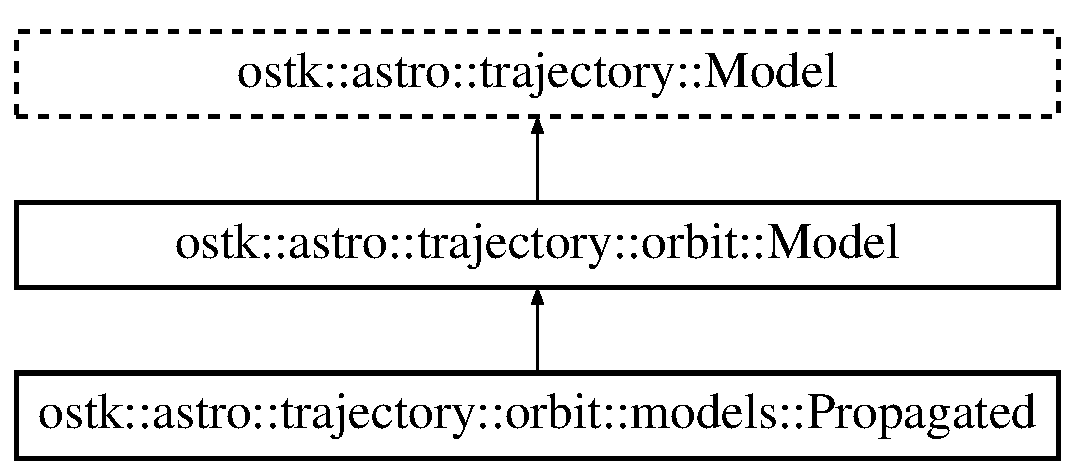
\includegraphics[height=3.000000cm]{classostk_1_1astro_1_1trajectory_1_1orbit_1_1models_1_1_propagated}
\end{center}
\end{figure}
\doxysubsection*{Public Member Functions}
\begin{DoxyCompactItemize}
\item 
\mbox{\hyperlink{classostk_1_1astro_1_1trajectory_1_1orbit_1_1models_1_1_propagated_aa7cbaccadc0e9cad5062545ef58cc439}{Propagated}} (const \mbox{\hyperlink{classostk_1_1astro_1_1trajectory_1_1_propagator}{Propagator}} \&a\+Propagator, const \mbox{\hyperlink{classostk_1_1astro_1_1trajectory_1_1_state}{State}} \&a\+State)
\begin{DoxyCompactList}\small\item\em Constructor. \end{DoxyCompactList}\item 
\mbox{\hyperlink{classostk_1_1astro_1_1trajectory_1_1orbit_1_1models_1_1_propagated_aea48e20ef7b8c5fdcf1a6be94f63d83c}{Propagated}} (const \mbox{\hyperlink{classostk_1_1astro_1_1trajectory_1_1_propagator}{Propagator}} \&a\+Propagator, const Array$<$ \mbox{\hyperlink{classostk_1_1astro_1_1trajectory_1_1_state}{State}} $>$ \&a\+Cached\+State\+Array)
\begin{DoxyCompactList}\small\item\em Constructor with a cached state array. \end{DoxyCompactList}\item 
virtual \mbox{\hyperlink{classostk_1_1astro_1_1trajectory_1_1orbit_1_1models_1_1_propagated}{Propagated}} $\ast$ \mbox{\hyperlink{classostk_1_1astro_1_1trajectory_1_1orbit_1_1models_1_1_propagated_a283639d985495c05adb9e80edb91cd12}{clone}} () const override
\begin{DoxyCompactList}\small\item\em Clone propagated. \end{DoxyCompactList}\item 
bool \mbox{\hyperlink{classostk_1_1astro_1_1trajectory_1_1orbit_1_1models_1_1_propagated_a88777b83d939ca894a20af525db347b8}{operator==}} (const \mbox{\hyperlink{classostk_1_1astro_1_1trajectory_1_1orbit_1_1models_1_1_propagated}{Propagated}} \&a\+Propagated\+Model) const
\begin{DoxyCompactList}\small\item\em Equal to operator. \end{DoxyCompactList}\item 
bool \mbox{\hyperlink{classostk_1_1astro_1_1trajectory_1_1orbit_1_1models_1_1_propagated_a71c17288a6039ddcc1a5d3e5e62e1f35}{operator!=}} (const \mbox{\hyperlink{classostk_1_1astro_1_1trajectory_1_1orbit_1_1models_1_1_propagated}{Propagated}} \&a\+Propagated\+Model) const
\begin{DoxyCompactList}\small\item\em Not equal to operator. \end{DoxyCompactList}\item 
virtual bool \mbox{\hyperlink{classostk_1_1astro_1_1trajectory_1_1orbit_1_1models_1_1_propagated_a530fd6bc017c74dedc43ced5fe843a03}{is\+Defined}} () const override
\begin{DoxyCompactList}\small\item\em Check if propagated model is defined. \end{DoxyCompactList}\item 
virtual Instant \mbox{\hyperlink{classostk_1_1astro_1_1trajectory_1_1orbit_1_1models_1_1_propagated_a3bf49ac0824e10057b6abca2cfcc692f}{get\+Epoch}} () const override
\begin{DoxyCompactList}\small\item\em Get epoch (in this case it is the first instant in the cached state array) \end{DoxyCompactList}\item 
virtual Integer \mbox{\hyperlink{classostk_1_1astro_1_1trajectory_1_1orbit_1_1models_1_1_propagated_a789e4236d2b8b212b1d978055b76abf1}{get\+Revolution\+Number\+At\+Epoch}} () const override
\begin{DoxyCompactList}\small\item\em Get revolution number at epoch (it is equal to 1) \end{DoxyCompactList}\item 
virtual \mbox{\hyperlink{classostk_1_1astro_1_1trajectory_1_1_state}{State}} \mbox{\hyperlink{classostk_1_1astro_1_1trajectory_1_1orbit_1_1models_1_1_propagated_a2efc3c1af735dcf2ec622d056fa0a13f}{calculate\+State\+At}} (const Instant \&an\+Instant) const override
\begin{DoxyCompactList}\small\item\em Calculate the state at an instant, utilizing internal cached state array to propagated shortest amount of time. \end{DoxyCompactList}\item 
virtual Array$<$ \mbox{\hyperlink{classostk_1_1astro_1_1trajectory_1_1_state}{State}} $>$ \mbox{\hyperlink{classostk_1_1astro_1_1trajectory_1_1orbit_1_1models_1_1_propagated_a9a4097432d2c863aedead23d2d67a7a7}{calculate\+States\+At}} (const Array$<$ Instant $>$ \&an\+Instant\+Array) const override
\begin{DoxyCompactList}\small\item\em Calculate the state at an instant, given initial state. \end{DoxyCompactList}\item 
virtual Integer \mbox{\hyperlink{classostk_1_1astro_1_1trajectory_1_1orbit_1_1models_1_1_propagated_a6360392c65494aa42aadff58ec58e49c}{calculate\+Revolution\+Number\+At}} (const Instant \&an\+Instant) const override
\begin{DoxyCompactList}\small\item\em Calculate the revolution number at an instant. \end{DoxyCompactList}\item 
const Array$<$ \mbox{\hyperlink{classostk_1_1astro_1_1trajectory_1_1_state}{State}} $>$ \& \mbox{\hyperlink{classostk_1_1astro_1_1trajectory_1_1orbit_1_1models_1_1_propagated_ab13c196dcea01238b6e1997cb46ced2b}{access\+Cached\+State\+Array}} () const
\begin{DoxyCompactList}\small\item\em Fetch internal cached state array. \end{DoxyCompactList}\item 
const \mbox{\hyperlink{classostk_1_1astro_1_1trajectory_1_1_propagator}{Propagator}} \& \mbox{\hyperlink{classostk_1_1astro_1_1trajectory_1_1orbit_1_1models_1_1_propagated_aabd25012cfd543722032f5bab8c0a3a3}{access\+Propagator}} () const
\begin{DoxyCompactList}\small\item\em \mbox{\hyperlink{classostk_1_1astro_1_1_access}{Access}} propagator. \end{DoxyCompactList}\item 
void \mbox{\hyperlink{classostk_1_1astro_1_1trajectory_1_1orbit_1_1models_1_1_propagated_a42c39258f14a74520c99bb5477a521df}{set\+Cached\+State\+Array}} (const Array$<$ \mbox{\hyperlink{classostk_1_1astro_1_1trajectory_1_1_state}{State}} $>$ \&a\+State\+Array)
\begin{DoxyCompactList}\small\item\em Set internal cached state array manually. \end{DoxyCompactList}\item 
virtual void \mbox{\hyperlink{classostk_1_1astro_1_1trajectory_1_1orbit_1_1models_1_1_propagated_a2b8aa6ff5511dbe92e6a3e7f4dd6880b}{print}} (std\+::ostream \&an\+Output\+Stream, bool display\+Decorator=true) const override
\begin{DoxyCompactList}\small\item\em Print propagated. \end{DoxyCompactList}\end{DoxyCompactItemize}
\doxysubsection*{Protected Member Functions}
\begin{DoxyCompactItemize}
\item 
virtual bool \mbox{\hyperlink{classostk_1_1astro_1_1trajectory_1_1orbit_1_1models_1_1_propagated_a29b52ccf653fbd84699edab0f198f590}{operator==}} (const \mbox{\hyperlink{classostk_1_1astro_1_1trajectory_1_1_model}{trajectory\+::\+Model}} \&a\+Model) const override
\begin{DoxyCompactList}\small\item\em Equal to operator. \end{DoxyCompactList}\item 
virtual bool \mbox{\hyperlink{classostk_1_1astro_1_1trajectory_1_1orbit_1_1models_1_1_propagated_aeffaddcde5540fd1226add8466415d08}{operator!=}} (const \mbox{\hyperlink{classostk_1_1astro_1_1trajectory_1_1_model}{trajectory\+::\+Model}} \&a\+Model) const override
\begin{DoxyCompactList}\small\item\em Not equal to operator. \end{DoxyCompactList}\end{DoxyCompactItemize}
\doxysubsection*{Friends}
\begin{DoxyCompactItemize}
\item 
std\+::ostream \& \mbox{\hyperlink{classostk_1_1astro_1_1trajectory_1_1orbit_1_1models_1_1_propagated_aa61df3429a00e0f64a497af2c81075c0}{operator$<$$<$}} (std\+::ostream \&an\+Output\+Stream, const \mbox{\hyperlink{classostk_1_1astro_1_1trajectory_1_1orbit_1_1models_1_1_propagated}{Propagated}} \&a\+Propagated\+Model)
\begin{DoxyCompactList}\small\item\em Output stream operator. \end{DoxyCompactList}\end{DoxyCompactItemize}


\doxysubsection{Detailed Description}
Defines an orbit model that is propagated using numerical propagation. 

\doxysubsection{Constructor \& Destructor Documentation}
\mbox{\Hypertarget{classostk_1_1astro_1_1trajectory_1_1orbit_1_1models_1_1_propagated_aa7cbaccadc0e9cad5062545ef58cc439}\label{classostk_1_1astro_1_1trajectory_1_1orbit_1_1models_1_1_propagated_aa7cbaccadc0e9cad5062545ef58cc439}} 
\index{ostk::astro::trajectory::orbit::models::Propagated@{ostk::astro::trajectory::orbit::models::Propagated}!Propagated@{Propagated}}
\index{Propagated@{Propagated}!ostk::astro::trajectory::orbit::models::Propagated@{ostk::astro::trajectory::orbit::models::Propagated}}
\doxysubsubsection{\texorpdfstring{Propagated()}{Propagated()}\hspace{0.1cm}{\footnotesize\ttfamily [1/2]}}
{\footnotesize\ttfamily ostk\+::astro\+::trajectory\+::orbit\+::models\+::\+Propagated\+::\+Propagated (\begin{DoxyParamCaption}\item[{const \mbox{\hyperlink{classostk_1_1astro_1_1trajectory_1_1_propagator}{Propagator}} \&}]{a\+Propagator,  }\item[{const \mbox{\hyperlink{classostk_1_1astro_1_1trajectory_1_1_state}{State}} \&}]{a\+State }\end{DoxyParamCaption})}



Constructor. 


\begin{DoxyCode}{0}
\DoxyCodeLine{\mbox{\hyperlink{classostk_1_1astro_1_1trajectory_1_1orbit_1_1models_1_1_propagated_aa7cbaccadc0e9cad5062545ef58cc439}{Propagated}} propagated = \{ aPropagator, aState \} ;}
\end{DoxyCode}



\begin{DoxyParams}[1]{Parameters}
\mbox{\texttt{ in}}  & {\em a\+Propagator} & A propagator \\
\hline
\mbox{\texttt{ in}}  & {\em a\+State} & A state \\
\hline
\end{DoxyParams}
\mbox{\Hypertarget{classostk_1_1astro_1_1trajectory_1_1orbit_1_1models_1_1_propagated_aea48e20ef7b8c5fdcf1a6be94f63d83c}\label{classostk_1_1astro_1_1trajectory_1_1orbit_1_1models_1_1_propagated_aea48e20ef7b8c5fdcf1a6be94f63d83c}} 
\index{ostk::astro::trajectory::orbit::models::Propagated@{ostk::astro::trajectory::orbit::models::Propagated}!Propagated@{Propagated}}
\index{Propagated@{Propagated}!ostk::astro::trajectory::orbit::models::Propagated@{ostk::astro::trajectory::orbit::models::Propagated}}
\doxysubsubsection{\texorpdfstring{Propagated()}{Propagated()}\hspace{0.1cm}{\footnotesize\ttfamily [2/2]}}
{\footnotesize\ttfamily ostk\+::astro\+::trajectory\+::orbit\+::models\+::\+Propagated\+::\+Propagated (\begin{DoxyParamCaption}\item[{const \mbox{\hyperlink{classostk_1_1astro_1_1trajectory_1_1_propagator}{Propagator}} \&}]{a\+Propagator,  }\item[{const Array$<$ \mbox{\hyperlink{classostk_1_1astro_1_1trajectory_1_1_state}{State}} $>$ \&}]{a\+Cached\+State\+Array }\end{DoxyParamCaption})}



Constructor with a cached state array. 


\begin{DoxyCode}{0}
\DoxyCodeLine{\mbox{\hyperlink{classostk_1_1astro_1_1trajectory_1_1orbit_1_1models_1_1_propagated_aa7cbaccadc0e9cad5062545ef58cc439}{Propagated}} propagated = \{ aPropagator, aCachedStateArray \} ;}
\end{DoxyCode}



\begin{DoxyParams}[1]{Parameters}
\mbox{\texttt{ in}}  & {\em a\+Propagator} & A propagator \\
\hline
\mbox{\texttt{ in}}  & {\em a\+Cached\+State\+Array} & A state array \\
\hline
\end{DoxyParams}


\doxysubsection{Member Function Documentation}
\mbox{\Hypertarget{classostk_1_1astro_1_1trajectory_1_1orbit_1_1models_1_1_propagated_ab13c196dcea01238b6e1997cb46ced2b}\label{classostk_1_1astro_1_1trajectory_1_1orbit_1_1models_1_1_propagated_ab13c196dcea01238b6e1997cb46ced2b}} 
\index{ostk::astro::trajectory::orbit::models::Propagated@{ostk::astro::trajectory::orbit::models::Propagated}!accessCachedStateArray@{accessCachedStateArray}}
\index{accessCachedStateArray@{accessCachedStateArray}!ostk::astro::trajectory::orbit::models::Propagated@{ostk::astro::trajectory::orbit::models::Propagated}}
\doxysubsubsection{\texorpdfstring{accessCachedStateArray()}{accessCachedStateArray()}}
{\footnotesize\ttfamily const Array$<$ \mbox{\hyperlink{classostk_1_1astro_1_1trajectory_1_1_state}{State}} $>$ \& ostk\+::astro\+::trajectory\+::orbit\+::models\+::\+Propagated\+::access\+Cached\+State\+Array (\begin{DoxyParamCaption}{ }\end{DoxyParamCaption}) const}



Fetch internal cached state array. 


\begin{DoxyCode}{0}
\DoxyCodeLine{Array<State> stateArray = propagated.accessCachedStateArray() ;}
\end{DoxyCode}
 \begin{DoxyReturn}{Returns}
Array$<$\+State$>$\& 
\end{DoxyReturn}
\mbox{\Hypertarget{classostk_1_1astro_1_1trajectory_1_1orbit_1_1models_1_1_propagated_aabd25012cfd543722032f5bab8c0a3a3}\label{classostk_1_1astro_1_1trajectory_1_1orbit_1_1models_1_1_propagated_aabd25012cfd543722032f5bab8c0a3a3}} 
\index{ostk::astro::trajectory::orbit::models::Propagated@{ostk::astro::trajectory::orbit::models::Propagated}!accessPropagator@{accessPropagator}}
\index{accessPropagator@{accessPropagator}!ostk::astro::trajectory::orbit::models::Propagated@{ostk::astro::trajectory::orbit::models::Propagated}}
\doxysubsubsection{\texorpdfstring{accessPropagator()}{accessPropagator()}}
{\footnotesize\ttfamily const \mbox{\hyperlink{classostk_1_1astro_1_1trajectory_1_1_propagator}{Propagator}} \& ostk\+::astro\+::trajectory\+::orbit\+::models\+::\+Propagated\+::access\+Propagator (\begin{DoxyParamCaption}{ }\end{DoxyParamCaption}) const}



\mbox{\hyperlink{classostk_1_1astro_1_1_access}{Access}} propagator. 


\begin{DoxyCode}{0}
\DoxyCodeLine{Propagator propagator = propagated.accessPropagator() ;}
\end{DoxyCode}


\begin{DoxyReturn}{Returns}
\mbox{\hyperlink{classostk_1_1astro_1_1trajectory_1_1_propagator}{Propagator}} 
\end{DoxyReturn}
\mbox{\Hypertarget{classostk_1_1astro_1_1trajectory_1_1orbit_1_1models_1_1_propagated_a6360392c65494aa42aadff58ec58e49c}\label{classostk_1_1astro_1_1trajectory_1_1orbit_1_1models_1_1_propagated_a6360392c65494aa42aadff58ec58e49c}} 
\index{ostk::astro::trajectory::orbit::models::Propagated@{ostk::astro::trajectory::orbit::models::Propagated}!calculateRevolutionNumberAt@{calculateRevolutionNumberAt}}
\index{calculateRevolutionNumberAt@{calculateRevolutionNumberAt}!ostk::astro::trajectory::orbit::models::Propagated@{ostk::astro::trajectory::orbit::models::Propagated}}
\doxysubsubsection{\texorpdfstring{calculateRevolutionNumberAt()}{calculateRevolutionNumberAt()}}
{\footnotesize\ttfamily Integer ostk\+::astro\+::trajectory\+::orbit\+::models\+::\+Propagated\+::calculate\+Revolution\+Number\+At (\begin{DoxyParamCaption}\item[{const Instant \&}]{an\+Instant }\end{DoxyParamCaption}) const\hspace{0.3cm}{\ttfamily [override]}, {\ttfamily [virtual]}}



Calculate the revolution number at an instant. 


\begin{DoxyCode}{0}
\DoxyCodeLine{Integer integer = propagated.calculateRevolutionNumberAt(anInstant) ;}
\end{DoxyCode}
 
\begin{DoxyParams}[1]{Parameters}
\mbox{\texttt{ in}}  & {\em an\+Instant} & An instant \\
\hline
\end{DoxyParams}
\begin{DoxyReturn}{Returns}
Integer 
\end{DoxyReturn}


Implements \mbox{\hyperlink{classostk_1_1astro_1_1trajectory_1_1orbit_1_1_model_aeecf4cc22fa9c766801936c468cc52ac}{ostk\+::astro\+::trajectory\+::orbit\+::\+Model}}.

\mbox{\Hypertarget{classostk_1_1astro_1_1trajectory_1_1orbit_1_1models_1_1_propagated_a2efc3c1af735dcf2ec622d056fa0a13f}\label{classostk_1_1astro_1_1trajectory_1_1orbit_1_1models_1_1_propagated_a2efc3c1af735dcf2ec622d056fa0a13f}} 
\index{ostk::astro::trajectory::orbit::models::Propagated@{ostk::astro::trajectory::orbit::models::Propagated}!calculateStateAt@{calculateStateAt}}
\index{calculateStateAt@{calculateStateAt}!ostk::astro::trajectory::orbit::models::Propagated@{ostk::astro::trajectory::orbit::models::Propagated}}
\doxysubsubsection{\texorpdfstring{calculateStateAt()}{calculateStateAt()}}
{\footnotesize\ttfamily \mbox{\hyperlink{classostk_1_1astro_1_1trajectory_1_1_state}{State}} ostk\+::astro\+::trajectory\+::orbit\+::models\+::\+Propagated\+::calculate\+State\+At (\begin{DoxyParamCaption}\item[{const Instant \&}]{an\+Instant }\end{DoxyParamCaption}) const\hspace{0.3cm}{\ttfamily [override]}, {\ttfamily [virtual]}}



Calculate the state at an instant, utilizing internal cached state array to propagated shortest amount of time. 

Does not have macro-\/level sorting optimization, should not be used with disorded instant array 
\begin{DoxyCode}{0}
\DoxyCodeLine{State state = propagated.calculateStateAt(anInstant) ;}
\end{DoxyCode}
 
\begin{DoxyParams}[1]{Parameters}
\mbox{\texttt{ in}}  & {\em an\+Instant} & An instant \\
\hline
\end{DoxyParams}
\begin{DoxyReturn}{Returns}
\mbox{\hyperlink{classostk_1_1astro_1_1trajectory_1_1_state}{State}} 
\end{DoxyReturn}


Implements \mbox{\hyperlink{classostk_1_1astro_1_1trajectory_1_1orbit_1_1_model_a34a0d8979ec1f7ade3e434fc0dad3711}{ostk\+::astro\+::trajectory\+::orbit\+::\+Model}}.

\mbox{\Hypertarget{classostk_1_1astro_1_1trajectory_1_1orbit_1_1models_1_1_propagated_a9a4097432d2c863aedead23d2d67a7a7}\label{classostk_1_1astro_1_1trajectory_1_1orbit_1_1models_1_1_propagated_a9a4097432d2c863aedead23d2d67a7a7}} 
\index{ostk::astro::trajectory::orbit::models::Propagated@{ostk::astro::trajectory::orbit::models::Propagated}!calculateStatesAt@{calculateStatesAt}}
\index{calculateStatesAt@{calculateStatesAt}!ostk::astro::trajectory::orbit::models::Propagated@{ostk::astro::trajectory::orbit::models::Propagated}}
\doxysubsubsection{\texorpdfstring{calculateStatesAt()}{calculateStatesAt()}}
{\footnotesize\ttfamily Array$<$ \mbox{\hyperlink{classostk_1_1astro_1_1trajectory_1_1_state}{State}} $>$ ostk\+::astro\+::trajectory\+::orbit\+::models\+::\+Propagated\+::calculate\+States\+At (\begin{DoxyParamCaption}\item[{const Array$<$ Instant $>$ \&}]{an\+Instant\+Array }\end{DoxyParamCaption}) const\hspace{0.3cm}{\ttfamily [override]}, {\ttfamily [virtual]}}



Calculate the state at an instant, given initial state. 


\begin{DoxyCode}{0}
\DoxyCodeLine{State state = propagated.calculateStateAt(aState, anInstant) ;}
\end{DoxyCode}
 
\begin{DoxyParams}[1]{Parameters}
\mbox{\texttt{ in}}  & {\em a\+State} & An initial state \\
\hline
\mbox{\texttt{ in}}  & {\em an\+Instant} & An instant \\
\hline
\end{DoxyParams}
\begin{DoxyReturn}{Returns}
\mbox{\hyperlink{classostk_1_1astro_1_1trajectory_1_1_state}{State}} 
\end{DoxyReturn}


Reimplemented from \mbox{\hyperlink{classostk_1_1astro_1_1trajectory_1_1_model_a3c3e4913aed2272174c0e6cd0d1a6415}{ostk\+::astro\+::trajectory\+::\+Model}}.

\mbox{\Hypertarget{classostk_1_1astro_1_1trajectory_1_1orbit_1_1models_1_1_propagated_a283639d985495c05adb9e80edb91cd12}\label{classostk_1_1astro_1_1trajectory_1_1orbit_1_1models_1_1_propagated_a283639d985495c05adb9e80edb91cd12}} 
\index{ostk::astro::trajectory::orbit::models::Propagated@{ostk::astro::trajectory::orbit::models::Propagated}!clone@{clone}}
\index{clone@{clone}!ostk::astro::trajectory::orbit::models::Propagated@{ostk::astro::trajectory::orbit::models::Propagated}}
\doxysubsubsection{\texorpdfstring{clone()}{clone()}}
{\footnotesize\ttfamily \mbox{\hyperlink{classostk_1_1astro_1_1trajectory_1_1orbit_1_1models_1_1_propagated}{Propagated}} $\ast$ ostk\+::astro\+::trajectory\+::orbit\+::models\+::\+Propagated\+::clone (\begin{DoxyParamCaption}{ }\end{DoxyParamCaption}) const\hspace{0.3cm}{\ttfamily [override]}, {\ttfamily [virtual]}}



Clone propagated. 

\begin{DoxyReturn}{Returns}
Pointer to cloned propagated 
\end{DoxyReturn}


Implements \mbox{\hyperlink{classostk_1_1astro_1_1trajectory_1_1orbit_1_1_model_a53dc07564e4c7c444da46360aa8ada15}{ostk\+::astro\+::trajectory\+::orbit\+::\+Model}}.

\mbox{\Hypertarget{classostk_1_1astro_1_1trajectory_1_1orbit_1_1models_1_1_propagated_a3bf49ac0824e10057b6abca2cfcc692f}\label{classostk_1_1astro_1_1trajectory_1_1orbit_1_1models_1_1_propagated_a3bf49ac0824e10057b6abca2cfcc692f}} 
\index{ostk::astro::trajectory::orbit::models::Propagated@{ostk::astro::trajectory::orbit::models::Propagated}!getEpoch@{getEpoch}}
\index{getEpoch@{getEpoch}!ostk::astro::trajectory::orbit::models::Propagated@{ostk::astro::trajectory::orbit::models::Propagated}}
\doxysubsubsection{\texorpdfstring{getEpoch()}{getEpoch()}}
{\footnotesize\ttfamily Instant ostk\+::astro\+::trajectory\+::orbit\+::models\+::\+Propagated\+::get\+Epoch (\begin{DoxyParamCaption}{ }\end{DoxyParamCaption}) const\hspace{0.3cm}{\ttfamily [override]}, {\ttfamily [virtual]}}



Get epoch (in this case it is the first instant in the cached state array) 


\begin{DoxyCode}{0}
\DoxyCodeLine{Instant instant = propagated.getEpoch() ;}
\end{DoxyCode}


\begin{DoxyReturn}{Returns}
Instant 
\end{DoxyReturn}


Implements \mbox{\hyperlink{classostk_1_1astro_1_1trajectory_1_1orbit_1_1_model_a22055d5ab4c22e6177a3ddb8f45f1f9b}{ostk\+::astro\+::trajectory\+::orbit\+::\+Model}}.

\mbox{\Hypertarget{classostk_1_1astro_1_1trajectory_1_1orbit_1_1models_1_1_propagated_a789e4236d2b8b212b1d978055b76abf1}\label{classostk_1_1astro_1_1trajectory_1_1orbit_1_1models_1_1_propagated_a789e4236d2b8b212b1d978055b76abf1}} 
\index{ostk::astro::trajectory::orbit::models::Propagated@{ostk::astro::trajectory::orbit::models::Propagated}!getRevolutionNumberAtEpoch@{getRevolutionNumberAtEpoch}}
\index{getRevolutionNumberAtEpoch@{getRevolutionNumberAtEpoch}!ostk::astro::trajectory::orbit::models::Propagated@{ostk::astro::trajectory::orbit::models::Propagated}}
\doxysubsubsection{\texorpdfstring{getRevolutionNumberAtEpoch()}{getRevolutionNumberAtEpoch()}}
{\footnotesize\ttfamily Integer ostk\+::astro\+::trajectory\+::orbit\+::models\+::\+Propagated\+::get\+Revolution\+Number\+At\+Epoch (\begin{DoxyParamCaption}{ }\end{DoxyParamCaption}) const\hspace{0.3cm}{\ttfamily [override]}, {\ttfamily [virtual]}}



Get revolution number at epoch (it is equal to 1) 


\begin{DoxyCode}{0}
\DoxyCodeLine{Real real = propagated.getRevolutionNumberAtEpoch() ;}
\end{DoxyCode}


\begin{DoxyReturn}{Returns}
Integer 
\end{DoxyReturn}


Implements \mbox{\hyperlink{classostk_1_1astro_1_1trajectory_1_1orbit_1_1_model_af3f1866f86045da2c05efe4165735cf4}{ostk\+::astro\+::trajectory\+::orbit\+::\+Model}}.

\mbox{\Hypertarget{classostk_1_1astro_1_1trajectory_1_1orbit_1_1models_1_1_propagated_a530fd6bc017c74dedc43ced5fe843a03}\label{classostk_1_1astro_1_1trajectory_1_1orbit_1_1models_1_1_propagated_a530fd6bc017c74dedc43ced5fe843a03}} 
\index{ostk::astro::trajectory::orbit::models::Propagated@{ostk::astro::trajectory::orbit::models::Propagated}!isDefined@{isDefined}}
\index{isDefined@{isDefined}!ostk::astro::trajectory::orbit::models::Propagated@{ostk::astro::trajectory::orbit::models::Propagated}}
\doxysubsubsection{\texorpdfstring{isDefined()}{isDefined()}}
{\footnotesize\ttfamily bool ostk\+::astro\+::trajectory\+::orbit\+::models\+::\+Propagated\+::is\+Defined (\begin{DoxyParamCaption}{ }\end{DoxyParamCaption}) const\hspace{0.3cm}{\ttfamily [override]}, {\ttfamily [virtual]}}



Check if propagated model is defined. 

\begin{DoxyReturn}{Returns}
True if propagated model is defined 
\end{DoxyReturn}


Implements \mbox{\hyperlink{classostk_1_1astro_1_1trajectory_1_1orbit_1_1_model_a13c5b5693dd86a072da0bd0e319bacc2}{ostk\+::astro\+::trajectory\+::orbit\+::\+Model}}.

\mbox{\Hypertarget{classostk_1_1astro_1_1trajectory_1_1orbit_1_1models_1_1_propagated_a71c17288a6039ddcc1a5d3e5e62e1f35}\label{classostk_1_1astro_1_1trajectory_1_1orbit_1_1models_1_1_propagated_a71c17288a6039ddcc1a5d3e5e62e1f35}} 
\index{ostk::astro::trajectory::orbit::models::Propagated@{ostk::astro::trajectory::orbit::models::Propagated}!operator"!=@{operator"!=}}
\index{operator"!=@{operator"!=}!ostk::astro::trajectory::orbit::models::Propagated@{ostk::astro::trajectory::orbit::models::Propagated}}
\doxysubsubsection{\texorpdfstring{operator"!=()}{operator!=()}\hspace{0.1cm}{\footnotesize\ttfamily [1/2]}}
{\footnotesize\ttfamily bool ostk\+::astro\+::trajectory\+::orbit\+::models\+::\+Propagated\+::operator!= (\begin{DoxyParamCaption}\item[{const \mbox{\hyperlink{classostk_1_1astro_1_1trajectory_1_1orbit_1_1models_1_1_propagated}{Propagated}} \&}]{a\+Propagated\+Model }\end{DoxyParamCaption}) const}



Not equal to operator. 


\begin{DoxyParams}[1]{Parameters}
\mbox{\texttt{ in}}  & {\em a\+Propagated\+Model} & A propagated \\
\hline
\end{DoxyParams}
\begin{DoxyReturn}{Returns}
True if propagateds are not equal 
\end{DoxyReturn}
\mbox{\Hypertarget{classostk_1_1astro_1_1trajectory_1_1orbit_1_1models_1_1_propagated_aeffaddcde5540fd1226add8466415d08}\label{classostk_1_1astro_1_1trajectory_1_1orbit_1_1models_1_1_propagated_aeffaddcde5540fd1226add8466415d08}} 
\index{ostk::astro::trajectory::orbit::models::Propagated@{ostk::astro::trajectory::orbit::models::Propagated}!operator"!=@{operator"!=}}
\index{operator"!=@{operator"!=}!ostk::astro::trajectory::orbit::models::Propagated@{ostk::astro::trajectory::orbit::models::Propagated}}
\doxysubsubsection{\texorpdfstring{operator"!=()}{operator!=()}\hspace{0.1cm}{\footnotesize\ttfamily [2/2]}}
{\footnotesize\ttfamily bool ostk\+::astro\+::trajectory\+::orbit\+::models\+::\+Propagated\+::operator!= (\begin{DoxyParamCaption}\item[{const \mbox{\hyperlink{classostk_1_1astro_1_1trajectory_1_1_model}{trajectory\+::\+Model}} \&}]{a\+Model }\end{DoxyParamCaption}) const\hspace{0.3cm}{\ttfamily [override]}, {\ttfamily [protected]}, {\ttfamily [virtual]}}



Not equal to operator. 


\begin{DoxyParams}[1]{Parameters}
\mbox{\texttt{ in}}  & {\em a\+Model} & A model \\
\hline
\end{DoxyParams}
\begin{DoxyReturn}{Returns}
True if models are not equal 
\end{DoxyReturn}


Implements \mbox{\hyperlink{classostk_1_1astro_1_1trajectory_1_1_model_a2dd77b9f6939d738f3a489f26c955340}{ostk\+::astro\+::trajectory\+::\+Model}}.

\mbox{\Hypertarget{classostk_1_1astro_1_1trajectory_1_1orbit_1_1models_1_1_propagated_a88777b83d939ca894a20af525db347b8}\label{classostk_1_1astro_1_1trajectory_1_1orbit_1_1models_1_1_propagated_a88777b83d939ca894a20af525db347b8}} 
\index{ostk::astro::trajectory::orbit::models::Propagated@{ostk::astro::trajectory::orbit::models::Propagated}!operator==@{operator==}}
\index{operator==@{operator==}!ostk::astro::trajectory::orbit::models::Propagated@{ostk::astro::trajectory::orbit::models::Propagated}}
\doxysubsubsection{\texorpdfstring{operator==()}{operator==()}\hspace{0.1cm}{\footnotesize\ttfamily [1/2]}}
{\footnotesize\ttfamily bool ostk\+::astro\+::trajectory\+::orbit\+::models\+::\+Propagated\+::operator== (\begin{DoxyParamCaption}\item[{const \mbox{\hyperlink{classostk_1_1astro_1_1trajectory_1_1orbit_1_1models_1_1_propagated}{Propagated}} \&}]{a\+Propagated\+Model }\end{DoxyParamCaption}) const}



Equal to operator. 


\begin{DoxyParams}[1]{Parameters}
\mbox{\texttt{ in}}  & {\em a\+Propagated\+Model} & A propagated \\
\hline
\end{DoxyParams}
\begin{DoxyReturn}{Returns}
True if propagateds are equal 
\end{DoxyReturn}
\mbox{\Hypertarget{classostk_1_1astro_1_1trajectory_1_1orbit_1_1models_1_1_propagated_a29b52ccf653fbd84699edab0f198f590}\label{classostk_1_1astro_1_1trajectory_1_1orbit_1_1models_1_1_propagated_a29b52ccf653fbd84699edab0f198f590}} 
\index{ostk::astro::trajectory::orbit::models::Propagated@{ostk::astro::trajectory::orbit::models::Propagated}!operator==@{operator==}}
\index{operator==@{operator==}!ostk::astro::trajectory::orbit::models::Propagated@{ostk::astro::trajectory::orbit::models::Propagated}}
\doxysubsubsection{\texorpdfstring{operator==()}{operator==()}\hspace{0.1cm}{\footnotesize\ttfamily [2/2]}}
{\footnotesize\ttfamily bool ostk\+::astro\+::trajectory\+::orbit\+::models\+::\+Propagated\+::operator== (\begin{DoxyParamCaption}\item[{const \mbox{\hyperlink{classostk_1_1astro_1_1trajectory_1_1_model}{trajectory\+::\+Model}} \&}]{a\+Model }\end{DoxyParamCaption}) const\hspace{0.3cm}{\ttfamily [override]}, {\ttfamily [protected]}, {\ttfamily [virtual]}}



Equal to operator. 


\begin{DoxyParams}[1]{Parameters}
\mbox{\texttt{ in}}  & {\em a\+Model} & A model \\
\hline
\end{DoxyParams}
\begin{DoxyReturn}{Returns}
True if models are equal 
\end{DoxyReturn}


Implements \mbox{\hyperlink{classostk_1_1astro_1_1trajectory_1_1_model_a874f79846e845859c070ce1b9874fc9c}{ostk\+::astro\+::trajectory\+::\+Model}}.

\mbox{\Hypertarget{classostk_1_1astro_1_1trajectory_1_1orbit_1_1models_1_1_propagated_a2b8aa6ff5511dbe92e6a3e7f4dd6880b}\label{classostk_1_1astro_1_1trajectory_1_1orbit_1_1models_1_1_propagated_a2b8aa6ff5511dbe92e6a3e7f4dd6880b}} 
\index{ostk::astro::trajectory::orbit::models::Propagated@{ostk::astro::trajectory::orbit::models::Propagated}!print@{print}}
\index{print@{print}!ostk::astro::trajectory::orbit::models::Propagated@{ostk::astro::trajectory::orbit::models::Propagated}}
\doxysubsubsection{\texorpdfstring{print()}{print()}}
{\footnotesize\ttfamily void ostk\+::astro\+::trajectory\+::orbit\+::models\+::\+Propagated\+::print (\begin{DoxyParamCaption}\item[{std\+::ostream \&}]{an\+Output\+Stream,  }\item[{bool}]{display\+Decorator = {\ttfamily true} }\end{DoxyParamCaption}) const\hspace{0.3cm}{\ttfamily [override]}, {\ttfamily [virtual]}}



Print propagated. 


\begin{DoxyParams}[1]{Parameters}
\mbox{\texttt{ in}}  & {\em an\+Output\+Stream} & An output stream \\
\hline
\mbox{\texttt{ in}}  & {\em (optional)} & display\+Decorators If true, display decorators \\
\hline
\end{DoxyParams}


Implements \mbox{\hyperlink{classostk_1_1astro_1_1trajectory_1_1orbit_1_1_model_a8ea45c1a6e51a6153ce3f72f5294f0c6}{ostk\+::astro\+::trajectory\+::orbit\+::\+Model}}.

\mbox{\Hypertarget{classostk_1_1astro_1_1trajectory_1_1orbit_1_1models_1_1_propagated_a42c39258f14a74520c99bb5477a521df}\label{classostk_1_1astro_1_1trajectory_1_1orbit_1_1models_1_1_propagated_a42c39258f14a74520c99bb5477a521df}} 
\index{ostk::astro::trajectory::orbit::models::Propagated@{ostk::astro::trajectory::orbit::models::Propagated}!setCachedStateArray@{setCachedStateArray}}
\index{setCachedStateArray@{setCachedStateArray}!ostk::astro::trajectory::orbit::models::Propagated@{ostk::astro::trajectory::orbit::models::Propagated}}
\doxysubsubsection{\texorpdfstring{setCachedStateArray()}{setCachedStateArray()}}
{\footnotesize\ttfamily void ostk\+::astro\+::trajectory\+::orbit\+::models\+::\+Propagated\+::set\+Cached\+State\+Array (\begin{DoxyParamCaption}\item[{const Array$<$ \mbox{\hyperlink{classostk_1_1astro_1_1trajectory_1_1_state}{State}} $>$ \&}]{a\+State\+Array }\end{DoxyParamCaption})}



Set internal cached state array manually. 


\begin{DoxyCode}{0}
\DoxyCodeLine{Array<State> stateArray = \{ ... \} ;}
\DoxyCodeLine{propagated.setCachedStateArray(stateArray) ;}
\end{DoxyCode}
 
\begin{DoxyParams}[1]{Parameters}
\mbox{\texttt{ in}}  & {\em a\+State\+Array} & A state array \\
\hline
\end{DoxyParams}


\doxysubsection{Friends And Related Function Documentation}
\mbox{\Hypertarget{classostk_1_1astro_1_1trajectory_1_1orbit_1_1models_1_1_propagated_aa61df3429a00e0f64a497af2c81075c0}\label{classostk_1_1astro_1_1trajectory_1_1orbit_1_1models_1_1_propagated_aa61df3429a00e0f64a497af2c81075c0}} 
\index{ostk::astro::trajectory::orbit::models::Propagated@{ostk::astro::trajectory::orbit::models::Propagated}!operator$<$$<$@{operator$<$$<$}}
\index{operator$<$$<$@{operator$<$$<$}!ostk::astro::trajectory::orbit::models::Propagated@{ostk::astro::trajectory::orbit::models::Propagated}}
\doxysubsubsection{\texorpdfstring{operator$<$$<$}{operator<<}}
{\footnotesize\ttfamily std\+::ostream\& operator$<$$<$ (\begin{DoxyParamCaption}\item[{std\+::ostream \&}]{an\+Output\+Stream,  }\item[{const \mbox{\hyperlink{classostk_1_1astro_1_1trajectory_1_1orbit_1_1models_1_1_propagated}{Propagated}} \&}]{a\+Propagated\+Model }\end{DoxyParamCaption})\hspace{0.3cm}{\ttfamily [friend]}}



Output stream operator. 


\begin{DoxyParams}[1]{Parameters}
\mbox{\texttt{ in}}  & {\em an\+Output\+Stream} & An output stream \\
\hline
\mbox{\texttt{ in}}  & {\em a\+Propagated\+Model} & A propagated model \\
\hline
\end{DoxyParams}
\begin{DoxyReturn}{Returns}
A reference to output stream 
\end{DoxyReturn}


The documentation for this class was generated from the following files\+:\begin{DoxyCompactItemize}
\item 
include/\+Open\+Space\+Toolkit/\+Astrodynamics/\+Trajectory/\+Orbit/\+Models/\mbox{\hyperlink{_propagated_8hpp}{Propagated.\+hpp}}\item 
src/\+Open\+Space\+Toolkit/\+Astrodynamics/\+Trajectory/\+Orbit/\+Models/\mbox{\hyperlink{_propagated_8cpp}{Propagated.\+cpp}}\end{DoxyCompactItemize}

\hypertarget{classostk_1_1astro_1_1trajectory_1_1_propagator}{}\doxysection{ostk\+::astro\+::trajectory\+::Propagator Class Reference}
\label{classostk_1_1astro_1_1trajectory_1_1_propagator}\index{ostk::astro::trajectory::Propagator@{ostk::astro::trajectory::Propagator}}


Defines a propagator to be used for numerical integration.  




{\ttfamily \#include $<$Propagator.\+hpp$>$}

\doxysubsection*{Public Member Functions}
\begin{DoxyCompactItemize}
\item 
\mbox{\hyperlink{classostk_1_1astro_1_1trajectory_1_1_propagator_a3e3802b0eaa96a0e9422db11a7deac16}{Propagator}} (const \mbox{\hyperlink{classostk_1_1astro_1_1flight_1_1system_1_1dynamics_1_1_satellite_dynamics}{Satellite\+Dynamics}} \&a\+Satellite\+Dynamics, const \mbox{\hyperlink{classostk_1_1astro_1_1_numerical_solver}{Numerical\+Solver}} \&a\+Numerical\+Solver)
\begin{DoxyCompactList}\small\item\em Constructor. \end{DoxyCompactList}\item 
\mbox{\hyperlink{classostk_1_1astro_1_1trajectory_1_1_propagator}{Propagator}} $\ast$ \mbox{\hyperlink{classostk_1_1astro_1_1trajectory_1_1_propagator_a9b21848949fad6f4f3f612a91c5c9106}{clone}} () const
\begin{DoxyCompactList}\small\item\em Clone propagator. \end{DoxyCompactList}\item 
bool \mbox{\hyperlink{classostk_1_1astro_1_1trajectory_1_1_propagator_aa16a98d76cd120299dd62e2f1e1c9bb9}{operator==}} (const \mbox{\hyperlink{classostk_1_1astro_1_1trajectory_1_1_propagator}{Propagator}} \&a\+Propagator) const
\begin{DoxyCompactList}\small\item\em Equal to operator. \end{DoxyCompactList}\item 
bool \mbox{\hyperlink{classostk_1_1astro_1_1trajectory_1_1_propagator_a2f4ddff27e509435d7d512f5fefc10c7}{operator!=}} (const \mbox{\hyperlink{classostk_1_1astro_1_1trajectory_1_1_propagator}{Propagator}} \&a\+Propagator) const
\begin{DoxyCompactList}\small\item\em Not equal to operator. \end{DoxyCompactList}\item 
bool \mbox{\hyperlink{classostk_1_1astro_1_1trajectory_1_1_propagator_a52140a4499899dda02e5c73179975e53}{is\+Defined}} () const
\begin{DoxyCompactList}\small\item\em Check if propagator is defined. \end{DoxyCompactList}\item 
\mbox{\hyperlink{classostk_1_1astro_1_1trajectory_1_1_state}{State}} \mbox{\hyperlink{classostk_1_1astro_1_1trajectory_1_1_propagator_aa0fde78b62924b7cf1eb81bf80bff165}{calculate\+State\+At}} (const \mbox{\hyperlink{classostk_1_1astro_1_1trajectory_1_1_state}{State}} \&a\+State, const Instant \&an\+Instant) const
\begin{DoxyCompactList}\small\item\em Calculate the state at an instant, given initial state. \end{DoxyCompactList}\item 
Array$<$ \mbox{\hyperlink{classostk_1_1astro_1_1trajectory_1_1_state}{State}} $>$ \mbox{\hyperlink{classostk_1_1astro_1_1trajectory_1_1_propagator_af61cfbdfeff89b32300f36c4346beee1}{calculate\+States\+At}} (const \mbox{\hyperlink{classostk_1_1astro_1_1trajectory_1_1_state}{State}} \&a\+State, const Array$<$ Instant $>$ \&an\+Instant\+Array) const
\begin{DoxyCompactList}\small\item\em Calculate the states at an array of instants, given an initial state. \end{DoxyCompactList}\item 
void \mbox{\hyperlink{classostk_1_1astro_1_1trajectory_1_1_propagator_afcd15a80e95284363dc51270db0777d6}{print}} (std\+::ostream \&an\+Output\+Stream, bool display\+Decorator=true) const
\begin{DoxyCompactList}\small\item\em Print propagator. \end{DoxyCompactList}\end{DoxyCompactItemize}
\doxysubsection*{Static Public Member Functions}
\begin{DoxyCompactItemize}
\item 
static \mbox{\hyperlink{classostk_1_1astro_1_1trajectory_1_1_propagator}{Propagator}} \mbox{\hyperlink{classostk_1_1astro_1_1trajectory_1_1_propagator_a8d807b90b10f02edb732afe28dca0c04}{Medium\+Fidelity}} ()
\begin{DoxyCompactList}\small\item\em Create a medium fidelity \mbox{\hyperlink{classostk_1_1astro_1_1trajectory_1_1_propagator}{Propagator}} object with recommended settings. \end{DoxyCompactList}\item 
static \mbox{\hyperlink{classostk_1_1astro_1_1trajectory_1_1_propagator}{Propagator}} \mbox{\hyperlink{classostk_1_1astro_1_1trajectory_1_1_propagator_ae49a22d28386d71da700c80b9a766983}{High\+Fidelity}} ()
\begin{DoxyCompactList}\small\item\em Create a high fidelity \mbox{\hyperlink{classostk_1_1astro_1_1trajectory_1_1_propagator}{Propagator}} object with recommended settings. \end{DoxyCompactList}\end{DoxyCompactItemize}
\doxysubsection*{Friends}
\begin{DoxyCompactItemize}
\item 
std\+::ostream \& \mbox{\hyperlink{classostk_1_1astro_1_1trajectory_1_1_propagator_a660922ef2c1c93694163c91686755257}{operator$<$$<$}} (std\+::ostream \&an\+Output\+Stream, const \mbox{\hyperlink{classostk_1_1astro_1_1trajectory_1_1_propagator}{Propagator}} \&a\+Propagator)
\begin{DoxyCompactList}\small\item\em Output stream operator. \end{DoxyCompactList}\end{DoxyCompactItemize}


\doxysubsection{Detailed Description}
Defines a propagator to be used for numerical integration. 

\doxysubsection{Constructor \& Destructor Documentation}
\mbox{\Hypertarget{classostk_1_1astro_1_1trajectory_1_1_propagator_a3e3802b0eaa96a0e9422db11a7deac16}\label{classostk_1_1astro_1_1trajectory_1_1_propagator_a3e3802b0eaa96a0e9422db11a7deac16}} 
\index{ostk::astro::trajectory::Propagator@{ostk::astro::trajectory::Propagator}!Propagator@{Propagator}}
\index{Propagator@{Propagator}!ostk::astro::trajectory::Propagator@{ostk::astro::trajectory::Propagator}}
\doxysubsubsection{\texorpdfstring{Propagator()}{Propagator()}}
{\footnotesize\ttfamily ostk\+::astro\+::trajectory\+::\+Propagator\+::\+Propagator (\begin{DoxyParamCaption}\item[{const \mbox{\hyperlink{classostk_1_1astro_1_1flight_1_1system_1_1dynamics_1_1_satellite_dynamics}{Satellite\+Dynamics}} \&}]{a\+Satellite\+Dynamics,  }\item[{const \mbox{\hyperlink{classostk_1_1astro_1_1_numerical_solver}{Numerical\+Solver}} \&}]{a\+Numerical\+Solver }\end{DoxyParamCaption})}



Constructor. 


\begin{DoxyCode}{0}
\DoxyCodeLine{\mbox{\hyperlink{classostk_1_1astro_1_1trajectory_1_1_propagator_a3e3802b0eaa96a0e9422db11a7deac16}{Propagator}} propagator = \{ aSatelliteDynamics, aNumericalSolver \} ;}
\end{DoxyCode}



\begin{DoxyParams}[1]{Parameters}
\mbox{\texttt{ in}}  & {\em a\+Satellite\+Dynamics} & A satellite dynamics object \\
\hline
\mbox{\texttt{ in}}  & {\em a\+Numerical\+Solver} & A numerical solver \\
\hline
\end{DoxyParams}


\doxysubsection{Member Function Documentation}
\mbox{\Hypertarget{classostk_1_1astro_1_1trajectory_1_1_propagator_aa0fde78b62924b7cf1eb81bf80bff165}\label{classostk_1_1astro_1_1trajectory_1_1_propagator_aa0fde78b62924b7cf1eb81bf80bff165}} 
\index{ostk::astro::trajectory::Propagator@{ostk::astro::trajectory::Propagator}!calculateStateAt@{calculateStateAt}}
\index{calculateStateAt@{calculateStateAt}!ostk::astro::trajectory::Propagator@{ostk::astro::trajectory::Propagator}}
\doxysubsubsection{\texorpdfstring{calculateStateAt()}{calculateStateAt()}}
{\footnotesize\ttfamily \mbox{\hyperlink{classostk_1_1astro_1_1trajectory_1_1_state}{State}} ostk\+::astro\+::trajectory\+::\+Propagator\+::calculate\+State\+At (\begin{DoxyParamCaption}\item[{const \mbox{\hyperlink{classostk_1_1astro_1_1trajectory_1_1_state}{State}} \&}]{a\+State,  }\item[{const Instant \&}]{an\+Instant }\end{DoxyParamCaption}) const}



Calculate the state at an instant, given initial state. 


\begin{DoxyCode}{0}
\DoxyCodeLine{State state = propagator.calculateStateAt(aState, anInstant) ;}
\end{DoxyCode}
 
\begin{DoxyParams}[1]{Parameters}
\mbox{\texttt{ in}}  & {\em a\+State} & An initial state \\
\hline
\mbox{\texttt{ in}}  & {\em an\+Instant} & An instant \\
\hline
\end{DoxyParams}
\begin{DoxyReturn}{Returns}
\mbox{\hyperlink{classostk_1_1astro_1_1trajectory_1_1_state}{State}} 
\end{DoxyReturn}
\mbox{\Hypertarget{classostk_1_1astro_1_1trajectory_1_1_propagator_af61cfbdfeff89b32300f36c4346beee1}\label{classostk_1_1astro_1_1trajectory_1_1_propagator_af61cfbdfeff89b32300f36c4346beee1}} 
\index{ostk::astro::trajectory::Propagator@{ostk::astro::trajectory::Propagator}!calculateStatesAt@{calculateStatesAt}}
\index{calculateStatesAt@{calculateStatesAt}!ostk::astro::trajectory::Propagator@{ostk::astro::trajectory::Propagator}}
\doxysubsubsection{\texorpdfstring{calculateStatesAt()}{calculateStatesAt()}}
{\footnotesize\ttfamily Array$<$ \mbox{\hyperlink{classostk_1_1astro_1_1trajectory_1_1_state}{State}} $>$ ostk\+::astro\+::trajectory\+::\+Propagator\+::calculate\+States\+At (\begin{DoxyParamCaption}\item[{const \mbox{\hyperlink{classostk_1_1astro_1_1trajectory_1_1_state}{State}} \&}]{a\+State,  }\item[{const Array$<$ Instant $>$ \&}]{an\+Instant\+Array }\end{DoxyParamCaption}) const}



Calculate the states at an array of instants, given an initial state. 

Can only be used with sorted instant array 
\begin{DoxyCode}{0}
\DoxyCodeLine{Array<State> states = propagator.calculateStatesAt(aState, anInstantArray) ;}
\end{DoxyCode}
 
\begin{DoxyParams}[1]{Parameters}
\mbox{\texttt{ in}}  & {\em an\+Instant\+Array} & An instant array \\
\hline
\end{DoxyParams}
\begin{DoxyReturn}{Returns}
Array$<$\+State$>$ 
\end{DoxyReturn}
\mbox{\Hypertarget{classostk_1_1astro_1_1trajectory_1_1_propagator_a9b21848949fad6f4f3f612a91c5c9106}\label{classostk_1_1astro_1_1trajectory_1_1_propagator_a9b21848949fad6f4f3f612a91c5c9106}} 
\index{ostk::astro::trajectory::Propagator@{ostk::astro::trajectory::Propagator}!clone@{clone}}
\index{clone@{clone}!ostk::astro::trajectory::Propagator@{ostk::astro::trajectory::Propagator}}
\doxysubsubsection{\texorpdfstring{clone()}{clone()}}
{\footnotesize\ttfamily \mbox{\hyperlink{classostk_1_1astro_1_1trajectory_1_1_propagator}{Propagator}} $\ast$ ostk\+::astro\+::trajectory\+::\+Propagator\+::clone (\begin{DoxyParamCaption}{ }\end{DoxyParamCaption}) const}



Clone propagator. 

\begin{DoxyReturn}{Returns}
Pointer to cloned propagator 
\end{DoxyReturn}
\mbox{\Hypertarget{classostk_1_1astro_1_1trajectory_1_1_propagator_ae49a22d28386d71da700c80b9a766983}\label{classostk_1_1astro_1_1trajectory_1_1_propagator_ae49a22d28386d71da700c80b9a766983}} 
\index{ostk::astro::trajectory::Propagator@{ostk::astro::trajectory::Propagator}!HighFidelity@{HighFidelity}}
\index{HighFidelity@{HighFidelity}!ostk::astro::trajectory::Propagator@{ostk::astro::trajectory::Propagator}}
\doxysubsubsection{\texorpdfstring{HighFidelity()}{HighFidelity()}}
{\footnotesize\ttfamily \mbox{\hyperlink{classostk_1_1astro_1_1trajectory_1_1_propagator}{Propagator}} ostk\+::astro\+::trajectory\+::\+Propagator\+::\+High\+Fidelity (\begin{DoxyParamCaption}{ }\end{DoxyParamCaption})\hspace{0.3cm}{\ttfamily [static]}}



Create a high fidelity \mbox{\hyperlink{classostk_1_1astro_1_1trajectory_1_1_propagator}{Propagator}} object with recommended settings. 


\begin{DoxyCode}{0}
\DoxyCodeLine{\mbox{\hyperlink{classostk_1_1astro_1_1trajectory_1_1_propagator_a3e3802b0eaa96a0e9422db11a7deac16}{Propagator}} propagator = \mbox{\hyperlink{classostk_1_1astro_1_1trajectory_1_1_propagator_ae49a22d28386d71da700c80b9a766983}{Propagator::HighFidelity}}(aState) ;}
\end{DoxyCode}
 
\begin{DoxyParams}[1]{Parameters}
\mbox{\texttt{ in}}  & {\em a\+State} & A \mbox{\hyperlink{classostk_1_1astro_1_1trajectory_1_1_state}{State}} \\
\hline
\end{DoxyParams}
\begin{DoxyReturn}{Returns}
\mbox{\hyperlink{classostk_1_1astro_1_1trajectory_1_1_propagator}{Propagator}} 
\end{DoxyReturn}
\mbox{\Hypertarget{classostk_1_1astro_1_1trajectory_1_1_propagator_a52140a4499899dda02e5c73179975e53}\label{classostk_1_1astro_1_1trajectory_1_1_propagator_a52140a4499899dda02e5c73179975e53}} 
\index{ostk::astro::trajectory::Propagator@{ostk::astro::trajectory::Propagator}!isDefined@{isDefined}}
\index{isDefined@{isDefined}!ostk::astro::trajectory::Propagator@{ostk::astro::trajectory::Propagator}}
\doxysubsubsection{\texorpdfstring{isDefined()}{isDefined()}}
{\footnotesize\ttfamily bool ostk\+::astro\+::trajectory\+::\+Propagator\+::is\+Defined (\begin{DoxyParamCaption}{ }\end{DoxyParamCaption}) const}



Check if propagator is defined. 

\begin{DoxyReturn}{Returns}
True if propagator is defined 
\end{DoxyReturn}
\mbox{\Hypertarget{classostk_1_1astro_1_1trajectory_1_1_propagator_a8d807b90b10f02edb732afe28dca0c04}\label{classostk_1_1astro_1_1trajectory_1_1_propagator_a8d807b90b10f02edb732afe28dca0c04}} 
\index{ostk::astro::trajectory::Propagator@{ostk::astro::trajectory::Propagator}!MediumFidelity@{MediumFidelity}}
\index{MediumFidelity@{MediumFidelity}!ostk::astro::trajectory::Propagator@{ostk::astro::trajectory::Propagator}}
\doxysubsubsection{\texorpdfstring{MediumFidelity()}{MediumFidelity()}}
{\footnotesize\ttfamily \mbox{\hyperlink{classostk_1_1astro_1_1trajectory_1_1_propagator}{Propagator}} ostk\+::astro\+::trajectory\+::\+Propagator\+::\+Medium\+Fidelity (\begin{DoxyParamCaption}{ }\end{DoxyParamCaption})\hspace{0.3cm}{\ttfamily [static]}}



Create a medium fidelity \mbox{\hyperlink{classostk_1_1astro_1_1trajectory_1_1_propagator}{Propagator}} object with recommended settings. 


\begin{DoxyCode}{0}
\DoxyCodeLine{\mbox{\hyperlink{classostk_1_1astro_1_1trajectory_1_1_propagator_a3e3802b0eaa96a0e9422db11a7deac16}{Propagator}} propagator = \mbox{\hyperlink{classostk_1_1astro_1_1trajectory_1_1_propagator_a8d807b90b10f02edb732afe28dca0c04}{Propagator::MediumFidelity}}(aState) ;}
\end{DoxyCode}
 
\begin{DoxyParams}[1]{Parameters}
\mbox{\texttt{ in}}  & {\em a\+State} & A \mbox{\hyperlink{classostk_1_1astro_1_1trajectory_1_1_state}{State}} \\
\hline
\end{DoxyParams}
\begin{DoxyReturn}{Returns}
\mbox{\hyperlink{classostk_1_1astro_1_1trajectory_1_1_propagator}{Propagator}} 
\end{DoxyReturn}
\mbox{\Hypertarget{classostk_1_1astro_1_1trajectory_1_1_propagator_a2f4ddff27e509435d7d512f5fefc10c7}\label{classostk_1_1astro_1_1trajectory_1_1_propagator_a2f4ddff27e509435d7d512f5fefc10c7}} 
\index{ostk::astro::trajectory::Propagator@{ostk::astro::trajectory::Propagator}!operator"!=@{operator"!=}}
\index{operator"!=@{operator"!=}!ostk::astro::trajectory::Propagator@{ostk::astro::trajectory::Propagator}}
\doxysubsubsection{\texorpdfstring{operator"!=()}{operator!=()}}
{\footnotesize\ttfamily bool ostk\+::astro\+::trajectory\+::\+Propagator\+::operator!= (\begin{DoxyParamCaption}\item[{const \mbox{\hyperlink{classostk_1_1astro_1_1trajectory_1_1_propagator}{Propagator}} \&}]{a\+Propagator }\end{DoxyParamCaption}) const}



Not equal to operator. 


\begin{DoxyParams}[1]{Parameters}
\mbox{\texttt{ in}}  & {\em a\+Propagator} & A propagator \\
\hline
\end{DoxyParams}
\begin{DoxyReturn}{Returns}
True if propagators are not equal 
\end{DoxyReturn}
\mbox{\Hypertarget{classostk_1_1astro_1_1trajectory_1_1_propagator_aa16a98d76cd120299dd62e2f1e1c9bb9}\label{classostk_1_1astro_1_1trajectory_1_1_propagator_aa16a98d76cd120299dd62e2f1e1c9bb9}} 
\index{ostk::astro::trajectory::Propagator@{ostk::astro::trajectory::Propagator}!operator==@{operator==}}
\index{operator==@{operator==}!ostk::astro::trajectory::Propagator@{ostk::astro::trajectory::Propagator}}
\doxysubsubsection{\texorpdfstring{operator==()}{operator==()}}
{\footnotesize\ttfamily bool ostk\+::astro\+::trajectory\+::\+Propagator\+::operator== (\begin{DoxyParamCaption}\item[{const \mbox{\hyperlink{classostk_1_1astro_1_1trajectory_1_1_propagator}{Propagator}} \&}]{a\+Propagator }\end{DoxyParamCaption}) const}



Equal to operator. 


\begin{DoxyParams}[1]{Parameters}
\mbox{\texttt{ in}}  & {\em a\+Propagator} & A propagator \\
\hline
\end{DoxyParams}
\begin{DoxyReturn}{Returns}
True if propagators are equal 
\end{DoxyReturn}
\mbox{\Hypertarget{classostk_1_1astro_1_1trajectory_1_1_propagator_afcd15a80e95284363dc51270db0777d6}\label{classostk_1_1astro_1_1trajectory_1_1_propagator_afcd15a80e95284363dc51270db0777d6}} 
\index{ostk::astro::trajectory::Propagator@{ostk::astro::trajectory::Propagator}!print@{print}}
\index{print@{print}!ostk::astro::trajectory::Propagator@{ostk::astro::trajectory::Propagator}}
\doxysubsubsection{\texorpdfstring{print()}{print()}}
{\footnotesize\ttfamily void ostk\+::astro\+::trajectory\+::\+Propagator\+::print (\begin{DoxyParamCaption}\item[{std\+::ostream \&}]{an\+Output\+Stream,  }\item[{bool}]{display\+Decorator = {\ttfamily true} }\end{DoxyParamCaption}) const}



Print propagator. 


\begin{DoxyParams}[1]{Parameters}
\mbox{\texttt{ in}}  & {\em an\+Output\+Stream} & An output stream \\
\hline
\mbox{\texttt{ in}}  & {\em (optional)} & display\+Decorators If true, display decorators \\
\hline
\end{DoxyParams}


\doxysubsection{Friends And Related Function Documentation}
\mbox{\Hypertarget{classostk_1_1astro_1_1trajectory_1_1_propagator_a660922ef2c1c93694163c91686755257}\label{classostk_1_1astro_1_1trajectory_1_1_propagator_a660922ef2c1c93694163c91686755257}} 
\index{ostk::astro::trajectory::Propagator@{ostk::astro::trajectory::Propagator}!operator$<$$<$@{operator$<$$<$}}
\index{operator$<$$<$@{operator$<$$<$}!ostk::astro::trajectory::Propagator@{ostk::astro::trajectory::Propagator}}
\doxysubsubsection{\texorpdfstring{operator$<$$<$}{operator<<}}
{\footnotesize\ttfamily std\+::ostream\& operator$<$$<$ (\begin{DoxyParamCaption}\item[{std\+::ostream \&}]{an\+Output\+Stream,  }\item[{const \mbox{\hyperlink{classostk_1_1astro_1_1trajectory_1_1_propagator}{Propagator}} \&}]{a\+Propagator }\end{DoxyParamCaption})\hspace{0.3cm}{\ttfamily [friend]}}



Output stream operator. 


\begin{DoxyParams}[1]{Parameters}
\mbox{\texttt{ in}}  & {\em an\+Output\+Stream} & An output stream \\
\hline
\mbox{\texttt{ in}}  & {\em a\+Propagator} & A propagator \\
\hline
\end{DoxyParams}
\begin{DoxyReturn}{Returns}
A reference to output stream 
\end{DoxyReturn}


The documentation for this class was generated from the following files\+:\begin{DoxyCompactItemize}
\item 
include/\+Open\+Space\+Toolkit/\+Astrodynamics/\+Trajectory/\mbox{\hyperlink{_propagator_8hpp}{Propagator.\+hpp}}\item 
src/\+Open\+Space\+Toolkit/\+Astrodynamics/\+Trajectory/\mbox{\hyperlink{_propagator_8cpp}{Propagator.\+cpp}}\end{DoxyCompactItemize}

\hypertarget{structostk_1_1astro_1_1conjunction_1_1messages_1_1ccsds_1_1_c_d_m_1_1_relative_metadata}{}\doxysection{ostk\+::astro\+::conjunction\+::messages\+::ccsds\+::C\+DM\+::Relative\+Metadata Struct Reference}
\label{structostk_1_1astro_1_1conjunction_1_1messages_1_1ccsds_1_1_c_d_m_1_1_relative_metadata}\index{ostk::astro::conjunction::messages::ccsds::CDM::RelativeMetadata@{ostk::astro::conjunction::messages::ccsds::CDM::RelativeMetadata}}


{\ttfamily \#include $<$C\+D\+M.\+hpp$>$}

\doxysubsection*{Public Attributes}
\begin{DoxyCompactItemize}
\item 
String \mbox{\hyperlink{structostk_1_1astro_1_1conjunction_1_1messages_1_1ccsds_1_1_c_d_m_1_1_relative_metadata_ab4c20facaf507c8968f1705ac09f67a5}{comment}} = String\+::\+Empty()
\item 
Instant \mbox{\hyperlink{structostk_1_1astro_1_1conjunction_1_1messages_1_1ccsds_1_1_c_d_m_1_1_relative_metadata_a5ff54bfc2f15a679244cc84cda3b5adc}{T\+CA}}
\item 
Length \mbox{\hyperlink{structostk_1_1astro_1_1conjunction_1_1messages_1_1ccsds_1_1_c_d_m_1_1_relative_metadata_a1196e463771c0f0199c4f54a1f1a05e7}{miss\+Distance}}
\item 
Position \mbox{\hyperlink{structostk_1_1astro_1_1conjunction_1_1messages_1_1ccsds_1_1_c_d_m_1_1_relative_metadata_a659e2e07a69047b7716bca49ff0d00f8}{relative\+Position}} = Position\+::\+Undefined()
\item 
Velocity \mbox{\hyperlink{structostk_1_1astro_1_1conjunction_1_1messages_1_1ccsds_1_1_c_d_m_1_1_relative_metadata_a2f1782200bd13c7a473769667a060870}{relative\+Velocity}} = Velocity\+::\+Undefined()
\item 
Instant \mbox{\hyperlink{structostk_1_1astro_1_1conjunction_1_1messages_1_1ccsds_1_1_c_d_m_1_1_relative_metadata_a41ed2de13d3990a54ee5184698e1df4a}{start\+Screen\+Period}} = Instant\+::\+Undefined()
\item 
Instant \mbox{\hyperlink{structostk_1_1astro_1_1conjunction_1_1messages_1_1ccsds_1_1_c_d_m_1_1_relative_metadata_a4131e67ee276fb8e09a814ef543dd7f0}{end\+Screen\+Period}} = Instant\+::\+Undefined()
\item 
String \mbox{\hyperlink{structostk_1_1astro_1_1conjunction_1_1messages_1_1ccsds_1_1_c_d_m_1_1_relative_metadata_aab6e00cedd6f308cdccf01d605659130}{screen\+Volume\+Frame}} = String\+::\+Empty()
\item 
String \mbox{\hyperlink{structostk_1_1astro_1_1conjunction_1_1messages_1_1ccsds_1_1_c_d_m_1_1_relative_metadata_a5c61458a82b76eb15898a9394921d540}{screen\+Volume\+Shape}} = String\+::\+Empty()
\item 
Real \mbox{\hyperlink{structostk_1_1astro_1_1conjunction_1_1messages_1_1ccsds_1_1_c_d_m_1_1_relative_metadata_a440c344301f3da0914287fc27efdecc3}{screen\+VolumeX}} = Real\+::\+Undefined()
\item 
Real \mbox{\hyperlink{structostk_1_1astro_1_1conjunction_1_1messages_1_1ccsds_1_1_c_d_m_1_1_relative_metadata_ac4af249795dd088566aad3eba225a140}{screen\+VolumeY}} = Real\+::\+Undefined()
\item 
Real \mbox{\hyperlink{structostk_1_1astro_1_1conjunction_1_1messages_1_1ccsds_1_1_c_d_m_1_1_relative_metadata_a9a8574e2bc75a5200ff14b90c231f700}{screen\+VolumeZ}} = Real\+::\+Undefined()
\item 
Instant \mbox{\hyperlink{structostk_1_1astro_1_1conjunction_1_1messages_1_1ccsds_1_1_c_d_m_1_1_relative_metadata_a66f0717458e9b17d7efd7db99c933f3f}{screen\+Entry\+Time}} = Instant\+::\+Undefined()
\item 
Instant \mbox{\hyperlink{structostk_1_1astro_1_1conjunction_1_1messages_1_1ccsds_1_1_c_d_m_1_1_relative_metadata_a4ec3cda5aff9fbd3b1037e5143c4e7c5}{screen\+Exit\+Time}} = Instant\+::\+Undefined()
\item 
Real \mbox{\hyperlink{structostk_1_1astro_1_1conjunction_1_1messages_1_1ccsds_1_1_c_d_m_1_1_relative_metadata_a86d304c892baba0130a1ca23e6eb9d3b}{collision\+Probability}} = Real\+::\+Undefined()
\item 
String \mbox{\hyperlink{structostk_1_1astro_1_1conjunction_1_1messages_1_1ccsds_1_1_c_d_m_1_1_relative_metadata_ad4a50fb4d316c140053d56e203985005}{collision\+Probability\+Method}} = String\+::\+Empty()
\end{DoxyCompactItemize}


\doxysubsection{Member Data Documentation}
\mbox{\Hypertarget{structostk_1_1astro_1_1conjunction_1_1messages_1_1ccsds_1_1_c_d_m_1_1_relative_metadata_a86d304c892baba0130a1ca23e6eb9d3b}\label{structostk_1_1astro_1_1conjunction_1_1messages_1_1ccsds_1_1_c_d_m_1_1_relative_metadata_a86d304c892baba0130a1ca23e6eb9d3b}} 
\index{ostk::astro::conjunction::messages::ccsds::CDM::RelativeMetadata@{ostk::astro::conjunction::messages::ccsds::CDM::RelativeMetadata}!collisionProbability@{collisionProbability}}
\index{collisionProbability@{collisionProbability}!ostk::astro::conjunction::messages::ccsds::CDM::RelativeMetadata@{ostk::astro::conjunction::messages::ccsds::CDM::RelativeMetadata}}
\doxysubsubsection{\texorpdfstring{collisionProbability}{collisionProbability}}
{\footnotesize\ttfamily Real ostk\+::astro\+::conjunction\+::messages\+::ccsds\+::\+C\+D\+M\+::\+Relative\+Metadata\+::collision\+Probability = Real\+::\+Undefined()}

\mbox{\Hypertarget{structostk_1_1astro_1_1conjunction_1_1messages_1_1ccsds_1_1_c_d_m_1_1_relative_metadata_ad4a50fb4d316c140053d56e203985005}\label{structostk_1_1astro_1_1conjunction_1_1messages_1_1ccsds_1_1_c_d_m_1_1_relative_metadata_ad4a50fb4d316c140053d56e203985005}} 
\index{ostk::astro::conjunction::messages::ccsds::CDM::RelativeMetadata@{ostk::astro::conjunction::messages::ccsds::CDM::RelativeMetadata}!collisionProbabilityMethod@{collisionProbabilityMethod}}
\index{collisionProbabilityMethod@{collisionProbabilityMethod}!ostk::astro::conjunction::messages::ccsds::CDM::RelativeMetadata@{ostk::astro::conjunction::messages::ccsds::CDM::RelativeMetadata}}
\doxysubsubsection{\texorpdfstring{collisionProbabilityMethod}{collisionProbabilityMethod}}
{\footnotesize\ttfamily String ostk\+::astro\+::conjunction\+::messages\+::ccsds\+::\+C\+D\+M\+::\+Relative\+Metadata\+::collision\+Probability\+Method = String\+::\+Empty()}

\mbox{\Hypertarget{structostk_1_1astro_1_1conjunction_1_1messages_1_1ccsds_1_1_c_d_m_1_1_relative_metadata_ab4c20facaf507c8968f1705ac09f67a5}\label{structostk_1_1astro_1_1conjunction_1_1messages_1_1ccsds_1_1_c_d_m_1_1_relative_metadata_ab4c20facaf507c8968f1705ac09f67a5}} 
\index{ostk::astro::conjunction::messages::ccsds::CDM::RelativeMetadata@{ostk::astro::conjunction::messages::ccsds::CDM::RelativeMetadata}!comment@{comment}}
\index{comment@{comment}!ostk::astro::conjunction::messages::ccsds::CDM::RelativeMetadata@{ostk::astro::conjunction::messages::ccsds::CDM::RelativeMetadata}}
\doxysubsubsection{\texorpdfstring{comment}{comment}}
{\footnotesize\ttfamily String ostk\+::astro\+::conjunction\+::messages\+::ccsds\+::\+C\+D\+M\+::\+Relative\+Metadata\+::comment = String\+::\+Empty()}

\mbox{\Hypertarget{structostk_1_1astro_1_1conjunction_1_1messages_1_1ccsds_1_1_c_d_m_1_1_relative_metadata_a4131e67ee276fb8e09a814ef543dd7f0}\label{structostk_1_1astro_1_1conjunction_1_1messages_1_1ccsds_1_1_c_d_m_1_1_relative_metadata_a4131e67ee276fb8e09a814ef543dd7f0}} 
\index{ostk::astro::conjunction::messages::ccsds::CDM::RelativeMetadata@{ostk::astro::conjunction::messages::ccsds::CDM::RelativeMetadata}!endScreenPeriod@{endScreenPeriod}}
\index{endScreenPeriod@{endScreenPeriod}!ostk::astro::conjunction::messages::ccsds::CDM::RelativeMetadata@{ostk::astro::conjunction::messages::ccsds::CDM::RelativeMetadata}}
\doxysubsubsection{\texorpdfstring{endScreenPeriod}{endScreenPeriod}}
{\footnotesize\ttfamily Instant ostk\+::astro\+::conjunction\+::messages\+::ccsds\+::\+C\+D\+M\+::\+Relative\+Metadata\+::end\+Screen\+Period = Instant\+::\+Undefined()}

\mbox{\Hypertarget{structostk_1_1astro_1_1conjunction_1_1messages_1_1ccsds_1_1_c_d_m_1_1_relative_metadata_a1196e463771c0f0199c4f54a1f1a05e7}\label{structostk_1_1astro_1_1conjunction_1_1messages_1_1ccsds_1_1_c_d_m_1_1_relative_metadata_a1196e463771c0f0199c4f54a1f1a05e7}} 
\index{ostk::astro::conjunction::messages::ccsds::CDM::RelativeMetadata@{ostk::astro::conjunction::messages::ccsds::CDM::RelativeMetadata}!missDistance@{missDistance}}
\index{missDistance@{missDistance}!ostk::astro::conjunction::messages::ccsds::CDM::RelativeMetadata@{ostk::astro::conjunction::messages::ccsds::CDM::RelativeMetadata}}
\doxysubsubsection{\texorpdfstring{missDistance}{missDistance}}
{\footnotesize\ttfamily Length ostk\+::astro\+::conjunction\+::messages\+::ccsds\+::\+C\+D\+M\+::\+Relative\+Metadata\+::miss\+Distance}

\mbox{\Hypertarget{structostk_1_1astro_1_1conjunction_1_1messages_1_1ccsds_1_1_c_d_m_1_1_relative_metadata_a659e2e07a69047b7716bca49ff0d00f8}\label{structostk_1_1astro_1_1conjunction_1_1messages_1_1ccsds_1_1_c_d_m_1_1_relative_metadata_a659e2e07a69047b7716bca49ff0d00f8}} 
\index{ostk::astro::conjunction::messages::ccsds::CDM::RelativeMetadata@{ostk::astro::conjunction::messages::ccsds::CDM::RelativeMetadata}!relativePosition@{relativePosition}}
\index{relativePosition@{relativePosition}!ostk::astro::conjunction::messages::ccsds::CDM::RelativeMetadata@{ostk::astro::conjunction::messages::ccsds::CDM::RelativeMetadata}}
\doxysubsubsection{\texorpdfstring{relativePosition}{relativePosition}}
{\footnotesize\ttfamily Position ostk\+::astro\+::conjunction\+::messages\+::ccsds\+::\+C\+D\+M\+::\+Relative\+Metadata\+::relative\+Position = Position\+::\+Undefined()}

\mbox{\Hypertarget{structostk_1_1astro_1_1conjunction_1_1messages_1_1ccsds_1_1_c_d_m_1_1_relative_metadata_a2f1782200bd13c7a473769667a060870}\label{structostk_1_1astro_1_1conjunction_1_1messages_1_1ccsds_1_1_c_d_m_1_1_relative_metadata_a2f1782200bd13c7a473769667a060870}} 
\index{ostk::astro::conjunction::messages::ccsds::CDM::RelativeMetadata@{ostk::astro::conjunction::messages::ccsds::CDM::RelativeMetadata}!relativeVelocity@{relativeVelocity}}
\index{relativeVelocity@{relativeVelocity}!ostk::astro::conjunction::messages::ccsds::CDM::RelativeMetadata@{ostk::astro::conjunction::messages::ccsds::CDM::RelativeMetadata}}
\doxysubsubsection{\texorpdfstring{relativeVelocity}{relativeVelocity}}
{\footnotesize\ttfamily Velocity ostk\+::astro\+::conjunction\+::messages\+::ccsds\+::\+C\+D\+M\+::\+Relative\+Metadata\+::relative\+Velocity = Velocity\+::\+Undefined()}

\mbox{\Hypertarget{structostk_1_1astro_1_1conjunction_1_1messages_1_1ccsds_1_1_c_d_m_1_1_relative_metadata_a66f0717458e9b17d7efd7db99c933f3f}\label{structostk_1_1astro_1_1conjunction_1_1messages_1_1ccsds_1_1_c_d_m_1_1_relative_metadata_a66f0717458e9b17d7efd7db99c933f3f}} 
\index{ostk::astro::conjunction::messages::ccsds::CDM::RelativeMetadata@{ostk::astro::conjunction::messages::ccsds::CDM::RelativeMetadata}!screenEntryTime@{screenEntryTime}}
\index{screenEntryTime@{screenEntryTime}!ostk::astro::conjunction::messages::ccsds::CDM::RelativeMetadata@{ostk::astro::conjunction::messages::ccsds::CDM::RelativeMetadata}}
\doxysubsubsection{\texorpdfstring{screenEntryTime}{screenEntryTime}}
{\footnotesize\ttfamily Instant ostk\+::astro\+::conjunction\+::messages\+::ccsds\+::\+C\+D\+M\+::\+Relative\+Metadata\+::screen\+Entry\+Time = Instant\+::\+Undefined()}

\mbox{\Hypertarget{structostk_1_1astro_1_1conjunction_1_1messages_1_1ccsds_1_1_c_d_m_1_1_relative_metadata_a4ec3cda5aff9fbd3b1037e5143c4e7c5}\label{structostk_1_1astro_1_1conjunction_1_1messages_1_1ccsds_1_1_c_d_m_1_1_relative_metadata_a4ec3cda5aff9fbd3b1037e5143c4e7c5}} 
\index{ostk::astro::conjunction::messages::ccsds::CDM::RelativeMetadata@{ostk::astro::conjunction::messages::ccsds::CDM::RelativeMetadata}!screenExitTime@{screenExitTime}}
\index{screenExitTime@{screenExitTime}!ostk::astro::conjunction::messages::ccsds::CDM::RelativeMetadata@{ostk::astro::conjunction::messages::ccsds::CDM::RelativeMetadata}}
\doxysubsubsection{\texorpdfstring{screenExitTime}{screenExitTime}}
{\footnotesize\ttfamily Instant ostk\+::astro\+::conjunction\+::messages\+::ccsds\+::\+C\+D\+M\+::\+Relative\+Metadata\+::screen\+Exit\+Time = Instant\+::\+Undefined()}

\mbox{\Hypertarget{structostk_1_1astro_1_1conjunction_1_1messages_1_1ccsds_1_1_c_d_m_1_1_relative_metadata_aab6e00cedd6f308cdccf01d605659130}\label{structostk_1_1astro_1_1conjunction_1_1messages_1_1ccsds_1_1_c_d_m_1_1_relative_metadata_aab6e00cedd6f308cdccf01d605659130}} 
\index{ostk::astro::conjunction::messages::ccsds::CDM::RelativeMetadata@{ostk::astro::conjunction::messages::ccsds::CDM::RelativeMetadata}!screenVolumeFrame@{screenVolumeFrame}}
\index{screenVolumeFrame@{screenVolumeFrame}!ostk::astro::conjunction::messages::ccsds::CDM::RelativeMetadata@{ostk::astro::conjunction::messages::ccsds::CDM::RelativeMetadata}}
\doxysubsubsection{\texorpdfstring{screenVolumeFrame}{screenVolumeFrame}}
{\footnotesize\ttfamily String ostk\+::astro\+::conjunction\+::messages\+::ccsds\+::\+C\+D\+M\+::\+Relative\+Metadata\+::screen\+Volume\+Frame = String\+::\+Empty()}

\mbox{\Hypertarget{structostk_1_1astro_1_1conjunction_1_1messages_1_1ccsds_1_1_c_d_m_1_1_relative_metadata_a5c61458a82b76eb15898a9394921d540}\label{structostk_1_1astro_1_1conjunction_1_1messages_1_1ccsds_1_1_c_d_m_1_1_relative_metadata_a5c61458a82b76eb15898a9394921d540}} 
\index{ostk::astro::conjunction::messages::ccsds::CDM::RelativeMetadata@{ostk::astro::conjunction::messages::ccsds::CDM::RelativeMetadata}!screenVolumeShape@{screenVolumeShape}}
\index{screenVolumeShape@{screenVolumeShape}!ostk::astro::conjunction::messages::ccsds::CDM::RelativeMetadata@{ostk::astro::conjunction::messages::ccsds::CDM::RelativeMetadata}}
\doxysubsubsection{\texorpdfstring{screenVolumeShape}{screenVolumeShape}}
{\footnotesize\ttfamily String ostk\+::astro\+::conjunction\+::messages\+::ccsds\+::\+C\+D\+M\+::\+Relative\+Metadata\+::screen\+Volume\+Shape = String\+::\+Empty()}

\mbox{\Hypertarget{structostk_1_1astro_1_1conjunction_1_1messages_1_1ccsds_1_1_c_d_m_1_1_relative_metadata_a440c344301f3da0914287fc27efdecc3}\label{structostk_1_1astro_1_1conjunction_1_1messages_1_1ccsds_1_1_c_d_m_1_1_relative_metadata_a440c344301f3da0914287fc27efdecc3}} 
\index{ostk::astro::conjunction::messages::ccsds::CDM::RelativeMetadata@{ostk::astro::conjunction::messages::ccsds::CDM::RelativeMetadata}!screenVolumeX@{screenVolumeX}}
\index{screenVolumeX@{screenVolumeX}!ostk::astro::conjunction::messages::ccsds::CDM::RelativeMetadata@{ostk::astro::conjunction::messages::ccsds::CDM::RelativeMetadata}}
\doxysubsubsection{\texorpdfstring{screenVolumeX}{screenVolumeX}}
{\footnotesize\ttfamily Real ostk\+::astro\+::conjunction\+::messages\+::ccsds\+::\+C\+D\+M\+::\+Relative\+Metadata\+::screen\+VolumeX = Real\+::\+Undefined()}

\mbox{\Hypertarget{structostk_1_1astro_1_1conjunction_1_1messages_1_1ccsds_1_1_c_d_m_1_1_relative_metadata_ac4af249795dd088566aad3eba225a140}\label{structostk_1_1astro_1_1conjunction_1_1messages_1_1ccsds_1_1_c_d_m_1_1_relative_metadata_ac4af249795dd088566aad3eba225a140}} 
\index{ostk::astro::conjunction::messages::ccsds::CDM::RelativeMetadata@{ostk::astro::conjunction::messages::ccsds::CDM::RelativeMetadata}!screenVolumeY@{screenVolumeY}}
\index{screenVolumeY@{screenVolumeY}!ostk::astro::conjunction::messages::ccsds::CDM::RelativeMetadata@{ostk::astro::conjunction::messages::ccsds::CDM::RelativeMetadata}}
\doxysubsubsection{\texorpdfstring{screenVolumeY}{screenVolumeY}}
{\footnotesize\ttfamily Real ostk\+::astro\+::conjunction\+::messages\+::ccsds\+::\+C\+D\+M\+::\+Relative\+Metadata\+::screen\+VolumeY = Real\+::\+Undefined()}

\mbox{\Hypertarget{structostk_1_1astro_1_1conjunction_1_1messages_1_1ccsds_1_1_c_d_m_1_1_relative_metadata_a9a8574e2bc75a5200ff14b90c231f700}\label{structostk_1_1astro_1_1conjunction_1_1messages_1_1ccsds_1_1_c_d_m_1_1_relative_metadata_a9a8574e2bc75a5200ff14b90c231f700}} 
\index{ostk::astro::conjunction::messages::ccsds::CDM::RelativeMetadata@{ostk::astro::conjunction::messages::ccsds::CDM::RelativeMetadata}!screenVolumeZ@{screenVolumeZ}}
\index{screenVolumeZ@{screenVolumeZ}!ostk::astro::conjunction::messages::ccsds::CDM::RelativeMetadata@{ostk::astro::conjunction::messages::ccsds::CDM::RelativeMetadata}}
\doxysubsubsection{\texorpdfstring{screenVolumeZ}{screenVolumeZ}}
{\footnotesize\ttfamily Real ostk\+::astro\+::conjunction\+::messages\+::ccsds\+::\+C\+D\+M\+::\+Relative\+Metadata\+::screen\+VolumeZ = Real\+::\+Undefined()}

\mbox{\Hypertarget{structostk_1_1astro_1_1conjunction_1_1messages_1_1ccsds_1_1_c_d_m_1_1_relative_metadata_a41ed2de13d3990a54ee5184698e1df4a}\label{structostk_1_1astro_1_1conjunction_1_1messages_1_1ccsds_1_1_c_d_m_1_1_relative_metadata_a41ed2de13d3990a54ee5184698e1df4a}} 
\index{ostk::astro::conjunction::messages::ccsds::CDM::RelativeMetadata@{ostk::astro::conjunction::messages::ccsds::CDM::RelativeMetadata}!startScreenPeriod@{startScreenPeriod}}
\index{startScreenPeriod@{startScreenPeriod}!ostk::astro::conjunction::messages::ccsds::CDM::RelativeMetadata@{ostk::astro::conjunction::messages::ccsds::CDM::RelativeMetadata}}
\doxysubsubsection{\texorpdfstring{startScreenPeriod}{startScreenPeriod}}
{\footnotesize\ttfamily Instant ostk\+::astro\+::conjunction\+::messages\+::ccsds\+::\+C\+D\+M\+::\+Relative\+Metadata\+::start\+Screen\+Period = Instant\+::\+Undefined()}

\mbox{\Hypertarget{structostk_1_1astro_1_1conjunction_1_1messages_1_1ccsds_1_1_c_d_m_1_1_relative_metadata_a5ff54bfc2f15a679244cc84cda3b5adc}\label{structostk_1_1astro_1_1conjunction_1_1messages_1_1ccsds_1_1_c_d_m_1_1_relative_metadata_a5ff54bfc2f15a679244cc84cda3b5adc}} 
\index{ostk::astro::conjunction::messages::ccsds::CDM::RelativeMetadata@{ostk::astro::conjunction::messages::ccsds::CDM::RelativeMetadata}!TCA@{TCA}}
\index{TCA@{TCA}!ostk::astro::conjunction::messages::ccsds::CDM::RelativeMetadata@{ostk::astro::conjunction::messages::ccsds::CDM::RelativeMetadata}}
\doxysubsubsection{\texorpdfstring{TCA}{TCA}}
{\footnotesize\ttfamily Instant ostk\+::astro\+::conjunction\+::messages\+::ccsds\+::\+C\+D\+M\+::\+Relative\+Metadata\+::\+T\+CA}



The documentation for this struct was generated from the following file\+:\begin{DoxyCompactItemize}
\item 
include/\+Open\+Space\+Toolkit/\+Astrodynamics/\+Conjunction/\+Messages/\+C\+C\+S\+D\+S/\mbox{\hyperlink{_c_d_m_8hpp}{C\+D\+M.\+hpp}}\end{DoxyCompactItemize}

\hypertarget{classostk_1_1astro_1_1flight_1_1system_1_1dynamics_1_1_satellite_dynamics}{}\doxysection{ostk\+::astro\+::flight\+::system\+::dynamics\+::Satellite\+Dynamics Class Reference}
\label{classostk_1_1astro_1_1flight_1_1system_1_1dynamics_1_1_satellite_dynamics}\index{ostk::astro::flight::system::dynamics::SatelliteDynamics@{ostk::astro::flight::system::dynamics::SatelliteDynamics}}


Defines a satellite in orbit subject to forces of varying fidelity Represents a system of differential equations that can be solved by calling the \mbox{\hyperlink{classostk_1_1astro_1_1_numerical_solver}{Numerical\+Solver}} class.  




{\ttfamily \#include $<$Satellite\+Dynamics.\+hpp$>$}

Inheritance diagram for ostk\+::astro\+::flight\+::system\+::dynamics\+::Satellite\+Dynamics\+:\begin{figure}[H]
\begin{center}
\leavevmode
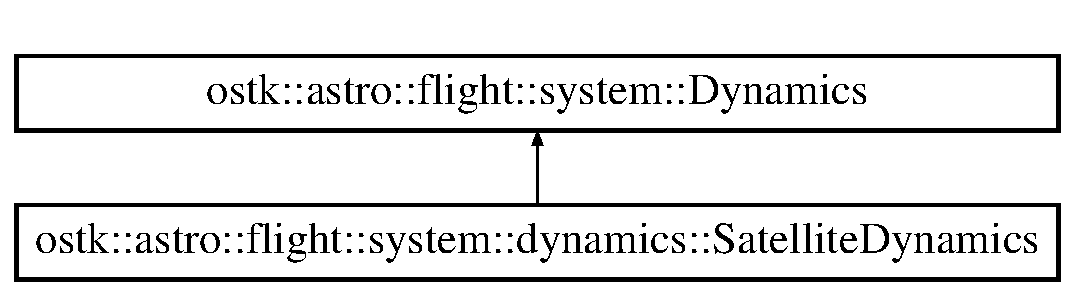
\includegraphics[height=2.000000cm]{classostk_1_1astro_1_1flight_1_1system_1_1dynamics_1_1_satellite_dynamics}
\end{center}
\end{figure}
\doxysubsection*{Public Member Functions}
\begin{DoxyCompactItemize}
\item 
\mbox{\hyperlink{classostk_1_1astro_1_1flight_1_1system_1_1dynamics_1_1_satellite_dynamics_a7bbf0ca2df46b4d1f9c2363010a2bd22}{Satellite\+Dynamics}} (const Environment \&an\+Environment, const \mbox{\hyperlink{classostk_1_1astro_1_1flight_1_1system_1_1_satellite_system}{Satellite\+System}} \&a\+Satellite\+System)
\begin{DoxyCompactList}\small\item\em Constructor. \end{DoxyCompactList}\item 
\mbox{\hyperlink{classostk_1_1astro_1_1flight_1_1system_1_1dynamics_1_1_satellite_dynamics_a8ced1fec7e36003eb50b8e15202fa571}{Satellite\+Dynamics}} (const \mbox{\hyperlink{classostk_1_1astro_1_1flight_1_1system_1_1dynamics_1_1_satellite_dynamics}{Satellite\+Dynamics}} \&a\+Satellite\+Dynamics)
\begin{DoxyCompactList}\small\item\em Copy Constructor. \end{DoxyCompactList}\item 
virtual \mbox{\hyperlink{classostk_1_1astro_1_1flight_1_1system_1_1dynamics_1_1_satellite_dynamics_a19f580468419341d3754707917aa835a}{$\sim$\+Satellite\+Dynamics}} () override
\begin{DoxyCompactList}\small\item\em Destructor. \end{DoxyCompactList}\item 
virtual \mbox{\hyperlink{classostk_1_1astro_1_1flight_1_1system_1_1dynamics_1_1_satellite_dynamics}{Satellite\+Dynamics}} $\ast$ \mbox{\hyperlink{classostk_1_1astro_1_1flight_1_1system_1_1dynamics_1_1_satellite_dynamics_a57d066e3876e999e288d00a23fb9ec9c}{clone}} () const override
\begin{DoxyCompactList}\small\item\em Clone satellite dynamics. \end{DoxyCompactList}\item 
bool \mbox{\hyperlink{classostk_1_1astro_1_1flight_1_1system_1_1dynamics_1_1_satellite_dynamics_a911f594991ee3b3a9187a34904118fc6}{operator==}} (const \mbox{\hyperlink{classostk_1_1astro_1_1flight_1_1system_1_1dynamics_1_1_satellite_dynamics}{Satellite\+Dynamics}} \&a\+Satellite\+Dynamics) const
\begin{DoxyCompactList}\small\item\em Equal to operator. \end{DoxyCompactList}\item 
bool \mbox{\hyperlink{classostk_1_1astro_1_1flight_1_1system_1_1dynamics_1_1_satellite_dynamics_a0f65a238480359b9baf68ea4b2155eda}{operator!=}} (const \mbox{\hyperlink{classostk_1_1astro_1_1flight_1_1system_1_1dynamics_1_1_satellite_dynamics}{Satellite\+Dynamics}} \&a\+Satellite\+Dynamics) const
\begin{DoxyCompactList}\small\item\em Not equal to operator. \end{DoxyCompactList}\item 
virtual bool \mbox{\hyperlink{classostk_1_1astro_1_1flight_1_1system_1_1dynamics_1_1_satellite_dynamics_aa58384471ec8825964af48a4a2235fab}{is\+Defined}} () const override
\begin{DoxyCompactList}\small\item\em Check if satellite dynamics is defined. \end{DoxyCompactList}\item 
virtual void \mbox{\hyperlink{classostk_1_1astro_1_1flight_1_1system_1_1dynamics_1_1_satellite_dynamics_af60a82bf97622e5b3a670c38ab4ddd32}{print}} (std\+::ostream \&an\+Output\+Stream, bool display\+Decorator=true) const override
\begin{DoxyCompactList}\small\item\em Print satellite dynamics. \end{DoxyCompactList}\item 
Instant \mbox{\hyperlink{classostk_1_1astro_1_1flight_1_1system_1_1dynamics_1_1_satellite_dynamics_ac8533e79bcab9b158940e49bd2723f95}{get\+Instant}} () const
\begin{DoxyCompactList}\small\item\em Get satellite dynamics initial instant. \end{DoxyCompactList}\item 
void \mbox{\hyperlink{classostk_1_1astro_1_1flight_1_1system_1_1dynamics_1_1_satellite_dynamics_ad1fe1ebe85ac3d5024032e42b4083c95}{set\+Instant}} (const Instant \&an\+Instant)
\begin{DoxyCompactList}\small\item\em Set satellite dynamics initial epoch. \end{DoxyCompactList}\item 
virtual \mbox{\hyperlink{classostk_1_1astro_1_1flight_1_1system_1_1_dynamics_a9b14f4fbea6fe1e96af9e71545d4c77e}{Dynamics\+::\+Dynamical\+Equation\+Wrapper}} \mbox{\hyperlink{classostk_1_1astro_1_1flight_1_1system_1_1dynamics_1_1_satellite_dynamics_aed9ddda1a1d1c4636e2c0d6ccc9d5a16}{get\+Dynamical\+Equations}} () override
\begin{DoxyCompactList}\small\item\em Obtain dynamical equations function wrapper. \end{DoxyCompactList}\end{DoxyCompactItemize}
\doxysubsection*{Friends}
\begin{DoxyCompactItemize}
\item 
std\+::ostream \& \mbox{\hyperlink{classostk_1_1astro_1_1flight_1_1system_1_1dynamics_1_1_satellite_dynamics_a26dfc3296b117e4887b254e5746b51bb}{operator$<$$<$}} (std\+::ostream \&an\+Output\+Stream, const \mbox{\hyperlink{classostk_1_1astro_1_1flight_1_1system_1_1dynamics_1_1_satellite_dynamics}{Satellite\+Dynamics}} \&a\+Satellite\+Dynamics)
\begin{DoxyCompactList}\small\item\em Output stream operator. \end{DoxyCompactList}\end{DoxyCompactItemize}
\doxysubsection*{Additional Inherited Members}


\doxysubsection{Detailed Description}
Defines a satellite in orbit subject to forces of varying fidelity Represents a system of differential equations that can be solved by calling the \mbox{\hyperlink{classostk_1_1astro_1_1_numerical_solver}{Numerical\+Solver}} class. 

\doxysubsection{Constructor \& Destructor Documentation}
\mbox{\Hypertarget{classostk_1_1astro_1_1flight_1_1system_1_1dynamics_1_1_satellite_dynamics_a7bbf0ca2df46b4d1f9c2363010a2bd22}\label{classostk_1_1astro_1_1flight_1_1system_1_1dynamics_1_1_satellite_dynamics_a7bbf0ca2df46b4d1f9c2363010a2bd22}} 
\index{ostk::astro::flight::system::dynamics::SatelliteDynamics@{ostk::astro::flight::system::dynamics::SatelliteDynamics}!SatelliteDynamics@{SatelliteDynamics}}
\index{SatelliteDynamics@{SatelliteDynamics}!ostk::astro::flight::system::dynamics::SatelliteDynamics@{ostk::astro::flight::system::dynamics::SatelliteDynamics}}
\doxysubsubsection{\texorpdfstring{SatelliteDynamics()}{SatelliteDynamics()}\hspace{0.1cm}{\footnotesize\ttfamily [1/2]}}
{\footnotesize\ttfamily ostk\+::astro\+::flight\+::system\+::dynamics\+::\+Satellite\+Dynamics\+::\+Satellite\+Dynamics (\begin{DoxyParamCaption}\item[{const Environment \&}]{an\+Environment,  }\item[{const \mbox{\hyperlink{classostk_1_1astro_1_1flight_1_1system_1_1_satellite_system}{Satellite\+System}} \&}]{a\+Satellite\+System }\end{DoxyParamCaption})}



Constructor. 


\begin{DoxyCode}{0}
\DoxyCodeLine{Environment environment = \{ ... \} ;}
\DoxyCodeLine{SatelliteSystem satelliteSystem = \{ ... \} ;}
\DoxyCodeLine{\mbox{\hyperlink{classostk_1_1astro_1_1flight_1_1system_1_1dynamics_1_1_satellite_dynamics_a7bbf0ca2df46b4d1f9c2363010a2bd22}{SatelliteDynamics}} satelliteDynamics = \{ environment, satelliteSystem \} ;}
\end{DoxyCode}



\begin{DoxyParams}[1]{Parameters}
\mbox{\texttt{ in}}  & {\em an\+Environment} & An environment \\
\hline
\mbox{\texttt{ in}}  & {\em a\+Satellite\+System} & A satellite system \\
\hline
\end{DoxyParams}
\mbox{\Hypertarget{classostk_1_1astro_1_1flight_1_1system_1_1dynamics_1_1_satellite_dynamics_a8ced1fec7e36003eb50b8e15202fa571}\label{classostk_1_1astro_1_1flight_1_1system_1_1dynamics_1_1_satellite_dynamics_a8ced1fec7e36003eb50b8e15202fa571}} 
\index{ostk::astro::flight::system::dynamics::SatelliteDynamics@{ostk::astro::flight::system::dynamics::SatelliteDynamics}!SatelliteDynamics@{SatelliteDynamics}}
\index{SatelliteDynamics@{SatelliteDynamics}!ostk::astro::flight::system::dynamics::SatelliteDynamics@{ostk::astro::flight::system::dynamics::SatelliteDynamics}}
\doxysubsubsection{\texorpdfstring{SatelliteDynamics()}{SatelliteDynamics()}\hspace{0.1cm}{\footnotesize\ttfamily [2/2]}}
{\footnotesize\ttfamily ostk\+::astro\+::flight\+::system\+::dynamics\+::\+Satellite\+Dynamics\+::\+Satellite\+Dynamics (\begin{DoxyParamCaption}\item[{const \mbox{\hyperlink{classostk_1_1astro_1_1flight_1_1system_1_1dynamics_1_1_satellite_dynamics}{Satellite\+Dynamics}} \&}]{a\+Satellite\+Dynamics }\end{DoxyParamCaption})}



Copy Constructor. 


\begin{DoxyParams}[1]{Parameters}
\mbox{\texttt{ in}}  & {\em \mbox{\hyperlink{classostk_1_1astro_1_1flight_1_1system_1_1dynamics_1_1_satellite_dynamics}{Satellite\+Dynamics}}} & A satellite dynamics \\
\hline
\end{DoxyParams}
\mbox{\Hypertarget{classostk_1_1astro_1_1flight_1_1system_1_1dynamics_1_1_satellite_dynamics_a19f580468419341d3754707917aa835a}\label{classostk_1_1astro_1_1flight_1_1system_1_1dynamics_1_1_satellite_dynamics_a19f580468419341d3754707917aa835a}} 
\index{ostk::astro::flight::system::dynamics::SatelliteDynamics@{ostk::astro::flight::system::dynamics::SatelliteDynamics}!````~SatelliteDynamics@{$\sim$SatelliteDynamics}}
\index{````~SatelliteDynamics@{$\sim$SatelliteDynamics}!ostk::astro::flight::system::dynamics::SatelliteDynamics@{ostk::astro::flight::system::dynamics::SatelliteDynamics}}
\doxysubsubsection{\texorpdfstring{$\sim$SatelliteDynamics()}{~SatelliteDynamics()}}
{\footnotesize\ttfamily ostk\+::astro\+::flight\+::system\+::dynamics\+::\+Satellite\+Dynamics\+::$\sim$\+Satellite\+Dynamics (\begin{DoxyParamCaption}{ }\end{DoxyParamCaption})\hspace{0.3cm}{\ttfamily [override]}, {\ttfamily [virtual]}}



Destructor. 



\doxysubsection{Member Function Documentation}
\mbox{\Hypertarget{classostk_1_1astro_1_1flight_1_1system_1_1dynamics_1_1_satellite_dynamics_a57d066e3876e999e288d00a23fb9ec9c}\label{classostk_1_1astro_1_1flight_1_1system_1_1dynamics_1_1_satellite_dynamics_a57d066e3876e999e288d00a23fb9ec9c}} 
\index{ostk::astro::flight::system::dynamics::SatelliteDynamics@{ostk::astro::flight::system::dynamics::SatelliteDynamics}!clone@{clone}}
\index{clone@{clone}!ostk::astro::flight::system::dynamics::SatelliteDynamics@{ostk::astro::flight::system::dynamics::SatelliteDynamics}}
\doxysubsubsection{\texorpdfstring{clone()}{clone()}}
{\footnotesize\ttfamily \mbox{\hyperlink{classostk_1_1astro_1_1flight_1_1system_1_1dynamics_1_1_satellite_dynamics}{Satellite\+Dynamics}} $\ast$ ostk\+::astro\+::flight\+::system\+::dynamics\+::\+Satellite\+Dynamics\+::clone (\begin{DoxyParamCaption}{ }\end{DoxyParamCaption}) const\hspace{0.3cm}{\ttfamily [override]}, {\ttfamily [virtual]}}



Clone satellite dynamics. 

\begin{DoxyReturn}{Returns}
Pointer to cloned satellite dynamics 
\end{DoxyReturn}


Implements \mbox{\hyperlink{classostk_1_1astro_1_1flight_1_1system_1_1_dynamics_a7de1a8ce101f3cee59fd624b487de5be}{ostk\+::astro\+::flight\+::system\+::\+Dynamics}}.

\mbox{\Hypertarget{classostk_1_1astro_1_1flight_1_1system_1_1dynamics_1_1_satellite_dynamics_aed9ddda1a1d1c4636e2c0d6ccc9d5a16}\label{classostk_1_1astro_1_1flight_1_1system_1_1dynamics_1_1_satellite_dynamics_aed9ddda1a1d1c4636e2c0d6ccc9d5a16}} 
\index{ostk::astro::flight::system::dynamics::SatelliteDynamics@{ostk::astro::flight::system::dynamics::SatelliteDynamics}!getDynamicalEquations@{getDynamicalEquations}}
\index{getDynamicalEquations@{getDynamicalEquations}!ostk::astro::flight::system::dynamics::SatelliteDynamics@{ostk::astro::flight::system::dynamics::SatelliteDynamics}}
\doxysubsubsection{\texorpdfstring{getDynamicalEquations()}{getDynamicalEquations()}}
{\footnotesize\ttfamily \mbox{\hyperlink{classostk_1_1astro_1_1flight_1_1system_1_1_dynamics_a9b14f4fbea6fe1e96af9e71545d4c77e}{Dynamics\+::\+Dynamical\+Equation\+Wrapper}} ostk\+::astro\+::flight\+::system\+::dynamics\+::\+Satellite\+Dynamics\+::get\+Dynamical\+Equations (\begin{DoxyParamCaption}{ }\end{DoxyParamCaption})\hspace{0.3cm}{\ttfamily [override]}, {\ttfamily [virtual]}}



Obtain dynamical equations function wrapper. 


\begin{DoxyCode}{0}
\DoxyCodeLine{\mbox{\hyperlink{classostk_1_1astro_1_1flight_1_1system_1_1_dynamics_a9b14f4fbea6fe1e96af9e71545d4c77e}{Dynamics::DynamicalEquationWrapper}} dyneq = satelliteDynamics.getDynamicalEquations() ;}
\end{DoxyCode}
 \begin{DoxyReturn}{Returns}
std\+::function$<$void(const std\+::vector$<$double$>$\&, std\+::vector$<$double$>$\&, const double)$>$ 
\end{DoxyReturn}


Implements \mbox{\hyperlink{classostk_1_1astro_1_1flight_1_1system_1_1_dynamics_a2001816629758bad7e960af54e87ddaa}{ostk\+::astro\+::flight\+::system\+::\+Dynamics}}.

\mbox{\Hypertarget{classostk_1_1astro_1_1flight_1_1system_1_1dynamics_1_1_satellite_dynamics_ac8533e79bcab9b158940e49bd2723f95}\label{classostk_1_1astro_1_1flight_1_1system_1_1dynamics_1_1_satellite_dynamics_ac8533e79bcab9b158940e49bd2723f95}} 
\index{ostk::astro::flight::system::dynamics::SatelliteDynamics@{ostk::astro::flight::system::dynamics::SatelliteDynamics}!getInstant@{getInstant}}
\index{getInstant@{getInstant}!ostk::astro::flight::system::dynamics::SatelliteDynamics@{ostk::astro::flight::system::dynamics::SatelliteDynamics}}
\doxysubsubsection{\texorpdfstring{getInstant()}{getInstant()}}
{\footnotesize\ttfamily Instant ostk\+::astro\+::flight\+::system\+::dynamics\+::\+Satellite\+Dynamics\+::get\+Instant (\begin{DoxyParamCaption}{ }\end{DoxyParamCaption}) const}



Get satellite dynamics initial instant. 


\begin{DoxyCode}{0}
\DoxyCodeLine{satelliteDynamics.getInstant() ;}
\end{DoxyCode}
 \mbox{\Hypertarget{classostk_1_1astro_1_1flight_1_1system_1_1dynamics_1_1_satellite_dynamics_aa58384471ec8825964af48a4a2235fab}\label{classostk_1_1astro_1_1flight_1_1system_1_1dynamics_1_1_satellite_dynamics_aa58384471ec8825964af48a4a2235fab}} 
\index{ostk::astro::flight::system::dynamics::SatelliteDynamics@{ostk::astro::flight::system::dynamics::SatelliteDynamics}!isDefined@{isDefined}}
\index{isDefined@{isDefined}!ostk::astro::flight::system::dynamics::SatelliteDynamics@{ostk::astro::flight::system::dynamics::SatelliteDynamics}}
\doxysubsubsection{\texorpdfstring{isDefined()}{isDefined()}}
{\footnotesize\ttfamily bool ostk\+::astro\+::flight\+::system\+::dynamics\+::\+Satellite\+Dynamics\+::is\+Defined (\begin{DoxyParamCaption}{ }\end{DoxyParamCaption}) const\hspace{0.3cm}{\ttfamily [override]}, {\ttfamily [virtual]}}



Check if satellite dynamics is defined. 

\begin{DoxyReturn}{Returns}
True if satellite dynamics is defined 
\end{DoxyReturn}


Implements \mbox{\hyperlink{classostk_1_1astro_1_1flight_1_1system_1_1_dynamics_a13160e001990a6ce8db807e39b8f97df}{ostk\+::astro\+::flight\+::system\+::\+Dynamics}}.

\mbox{\Hypertarget{classostk_1_1astro_1_1flight_1_1system_1_1dynamics_1_1_satellite_dynamics_a0f65a238480359b9baf68ea4b2155eda}\label{classostk_1_1astro_1_1flight_1_1system_1_1dynamics_1_1_satellite_dynamics_a0f65a238480359b9baf68ea4b2155eda}} 
\index{ostk::astro::flight::system::dynamics::SatelliteDynamics@{ostk::astro::flight::system::dynamics::SatelliteDynamics}!operator"!=@{operator"!=}}
\index{operator"!=@{operator"!=}!ostk::astro::flight::system::dynamics::SatelliteDynamics@{ostk::astro::flight::system::dynamics::SatelliteDynamics}}
\doxysubsubsection{\texorpdfstring{operator"!=()}{operator!=()}}
{\footnotesize\ttfamily bool ostk\+::astro\+::flight\+::system\+::dynamics\+::\+Satellite\+Dynamics\+::operator!= (\begin{DoxyParamCaption}\item[{const \mbox{\hyperlink{classostk_1_1astro_1_1flight_1_1system_1_1dynamics_1_1_satellite_dynamics}{Satellite\+Dynamics}} \&}]{a\+Satellite\+Dynamics }\end{DoxyParamCaption}) const}



Not equal to operator. 


\begin{DoxyParams}[1]{Parameters}
\mbox{\texttt{ in}}  & {\em a\+Satellite\+Dynamics} & A satellite dynamics \\
\hline
\end{DoxyParams}
\begin{DoxyReturn}{Returns}
True if satellite dynamics are not equal 
\end{DoxyReturn}
\mbox{\Hypertarget{classostk_1_1astro_1_1flight_1_1system_1_1dynamics_1_1_satellite_dynamics_a911f594991ee3b3a9187a34904118fc6}\label{classostk_1_1astro_1_1flight_1_1system_1_1dynamics_1_1_satellite_dynamics_a911f594991ee3b3a9187a34904118fc6}} 
\index{ostk::astro::flight::system::dynamics::SatelliteDynamics@{ostk::astro::flight::system::dynamics::SatelliteDynamics}!operator==@{operator==}}
\index{operator==@{operator==}!ostk::astro::flight::system::dynamics::SatelliteDynamics@{ostk::astro::flight::system::dynamics::SatelliteDynamics}}
\doxysubsubsection{\texorpdfstring{operator==()}{operator==()}}
{\footnotesize\ttfamily bool ostk\+::astro\+::flight\+::system\+::dynamics\+::\+Satellite\+Dynamics\+::operator== (\begin{DoxyParamCaption}\item[{const \mbox{\hyperlink{classostk_1_1astro_1_1flight_1_1system_1_1dynamics_1_1_satellite_dynamics}{Satellite\+Dynamics}} \&}]{a\+Satellite\+Dynamics }\end{DoxyParamCaption}) const}



Equal to operator. 


\begin{DoxyParams}[1]{Parameters}
\mbox{\texttt{ in}}  & {\em a\+Satellite\+Dynamics} & A satellite dynamics \\
\hline
\end{DoxyParams}
\begin{DoxyReturn}{Returns}
True if satellite dynamics are equal 
\end{DoxyReturn}
\mbox{\Hypertarget{classostk_1_1astro_1_1flight_1_1system_1_1dynamics_1_1_satellite_dynamics_af60a82bf97622e5b3a670c38ab4ddd32}\label{classostk_1_1astro_1_1flight_1_1system_1_1dynamics_1_1_satellite_dynamics_af60a82bf97622e5b3a670c38ab4ddd32}} 
\index{ostk::astro::flight::system::dynamics::SatelliteDynamics@{ostk::astro::flight::system::dynamics::SatelliteDynamics}!print@{print}}
\index{print@{print}!ostk::astro::flight::system::dynamics::SatelliteDynamics@{ostk::astro::flight::system::dynamics::SatelliteDynamics}}
\doxysubsubsection{\texorpdfstring{print()}{print()}}
{\footnotesize\ttfamily void ostk\+::astro\+::flight\+::system\+::dynamics\+::\+Satellite\+Dynamics\+::print (\begin{DoxyParamCaption}\item[{std\+::ostream \&}]{an\+Output\+Stream,  }\item[{bool}]{display\+Decorator = {\ttfamily true} }\end{DoxyParamCaption}) const\hspace{0.3cm}{\ttfamily [override]}, {\ttfamily [virtual]}}



Print satellite dynamics. 


\begin{DoxyParams}[1]{Parameters}
\mbox{\texttt{ in}}  & {\em an\+Output\+Stream} & An output stream \\
\hline
\mbox{\texttt{ in}}  & {\em (optional)} & display\+Decorators If true, display decorators \\
\hline
\end{DoxyParams}


Implements \mbox{\hyperlink{classostk_1_1astro_1_1flight_1_1system_1_1_dynamics_aa3fdfebb45a96bb0c6405c750e1c6d30}{ostk\+::astro\+::flight\+::system\+::\+Dynamics}}.

\mbox{\Hypertarget{classostk_1_1astro_1_1flight_1_1system_1_1dynamics_1_1_satellite_dynamics_ad1fe1ebe85ac3d5024032e42b4083c95}\label{classostk_1_1astro_1_1flight_1_1system_1_1dynamics_1_1_satellite_dynamics_ad1fe1ebe85ac3d5024032e42b4083c95}} 
\index{ostk::astro::flight::system::dynamics::SatelliteDynamics@{ostk::astro::flight::system::dynamics::SatelliteDynamics}!setInstant@{setInstant}}
\index{setInstant@{setInstant}!ostk::astro::flight::system::dynamics::SatelliteDynamics@{ostk::astro::flight::system::dynamics::SatelliteDynamics}}
\doxysubsubsection{\texorpdfstring{setInstant()}{setInstant()}}
{\footnotesize\ttfamily void ostk\+::astro\+::flight\+::system\+::dynamics\+::\+Satellite\+Dynamics\+::set\+Instant (\begin{DoxyParamCaption}\item[{const Instant \&}]{an\+Instant }\end{DoxyParamCaption})}



Set satellite dynamics initial epoch. 


\begin{DoxyCode}{0}
\DoxyCodeLine{Instant instant = \{ ... \} ;}
\DoxyCodeLine{satelliteDynamics.setInstant(instant) ;}
\end{DoxyCode}
 
\begin{DoxyParams}[1]{Parameters}
\mbox{\texttt{ in}}  & {\em an\+Instant} & An instant \\
\hline
\end{DoxyParams}


\doxysubsection{Friends And Related Function Documentation}
\mbox{\Hypertarget{classostk_1_1astro_1_1flight_1_1system_1_1dynamics_1_1_satellite_dynamics_a26dfc3296b117e4887b254e5746b51bb}\label{classostk_1_1astro_1_1flight_1_1system_1_1dynamics_1_1_satellite_dynamics_a26dfc3296b117e4887b254e5746b51bb}} 
\index{ostk::astro::flight::system::dynamics::SatelliteDynamics@{ostk::astro::flight::system::dynamics::SatelliteDynamics}!operator$<$$<$@{operator$<$$<$}}
\index{operator$<$$<$@{operator$<$$<$}!ostk::astro::flight::system::dynamics::SatelliteDynamics@{ostk::astro::flight::system::dynamics::SatelliteDynamics}}
\doxysubsubsection{\texorpdfstring{operator$<$$<$}{operator<<}}
{\footnotesize\ttfamily std\+::ostream\& operator$<$$<$ (\begin{DoxyParamCaption}\item[{std\+::ostream \&}]{an\+Output\+Stream,  }\item[{const \mbox{\hyperlink{classostk_1_1astro_1_1flight_1_1system_1_1dynamics_1_1_satellite_dynamics}{Satellite\+Dynamics}} \&}]{a\+Satellite\+Dynamics }\end{DoxyParamCaption})\hspace{0.3cm}{\ttfamily [friend]}}



Output stream operator. 


\begin{DoxyParams}[1]{Parameters}
\mbox{\texttt{ in}}  & {\em an\+Output\+Stream} & An output stream \\
\hline
\mbox{\texttt{ in}}  & {\em a\+Satellite\+Dynamics} & A satellite dynamics \\
\hline
\end{DoxyParams}
\begin{DoxyReturn}{Returns}
A reference to output stream 
\end{DoxyReturn}


The documentation for this class was generated from the following files\+:\begin{DoxyCompactItemize}
\item 
include/\+Open\+Space\+Toolkit/\+Astrodynamics/\+Flight/\+System/\+Dynamics/\mbox{\hyperlink{_satellite_dynamics_8hpp}{Satellite\+Dynamics.\+hpp}}\item 
src/\+Open\+Space\+Toolkit/\+Astrodynamics/\+Flight/\+System/\+Dynamics/\mbox{\hyperlink{_satellite_dynamics_8cpp}{Satellite\+Dynamics.\+cpp}}\end{DoxyCompactItemize}

\hypertarget{classostk_1_1astro_1_1flight_1_1system_1_1_satellite_system}{}\doxysection{ostk\+::astro\+::flight\+::system\+::Satellite\+System Class Reference}
\label{classostk_1_1astro_1_1flight_1_1system_1_1_satellite_system}\index{ostk::astro::flight::system::SatelliteSystem@{ostk::astro::flight::system::SatelliteSystem}}


Define the dynamics system who\textquotesingle{}s motion is being studied, in particular this is a satellite system.  




{\ttfamily \#include $<$Satellite\+System.\+hpp$>$}

Inheritance diagram for ostk\+::astro\+::flight\+::system\+::Satellite\+System\+:\begin{figure}[H]
\begin{center}
\leavevmode
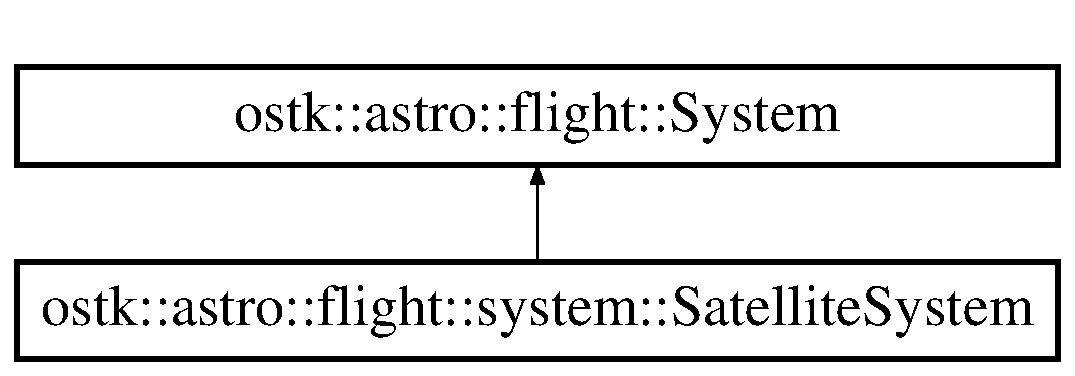
\includegraphics[height=2.000000cm]{classostk_1_1astro_1_1flight_1_1system_1_1_satellite_system}
\end{center}
\end{figure}
\doxysubsection*{Public Member Functions}
\begin{DoxyCompactItemize}
\item 
\mbox{\hyperlink{classostk_1_1astro_1_1flight_1_1system_1_1_satellite_system_a82127fe5971221429b8d18fcca9200f1}{Satellite\+System}} (const Mass \&a\+Dry\+Mass, const Composite \&a\+Satellite\+Geometry, const Matrix3d \&an\+Inertia\+Tensor, const Real \&a\+Cross\+Sectional\+Surface\+Area, const Real \&a\+Drag\+Coefficient, const \mbox{\hyperlink{classostk_1_1astro_1_1flight_1_1system_1_1_propulsion_system}{Propulsion\+System}} \&a\+Propulsion\+System=\mbox{\hyperlink{classostk_1_1astro_1_1flight_1_1system_1_1_propulsion_system_a1bccf402afccdcfdaf7445fc25e64bf4}{Propulsion\+System\+::\+Undefined}}())
\begin{DoxyCompactList}\small\item\em Constructor. \end{DoxyCompactList}\item 
virtual \mbox{\hyperlink{classostk_1_1astro_1_1flight_1_1system_1_1_satellite_system_a9d49e1a03773c4d78ba6dc579b24b713}{$\sim$\+Satellite\+System}} () override
\begin{DoxyCompactList}\small\item\em Destructor. \end{DoxyCompactList}\item 
\mbox{\hyperlink{classostk_1_1astro_1_1flight_1_1system_1_1_satellite_system}{Satellite\+System}} $\ast$ \mbox{\hyperlink{classostk_1_1astro_1_1flight_1_1system_1_1_satellite_system_ab72eb53f29c3f6f9839eaefd5667f218}{clone}} () const
\begin{DoxyCompactList}\small\item\em Clone satellite system. \end{DoxyCompactList}\item 
bool \mbox{\hyperlink{classostk_1_1astro_1_1flight_1_1system_1_1_satellite_system_aa74775f808a686c2452a9868d72ab5ef}{operator==}} (const \mbox{\hyperlink{classostk_1_1astro_1_1flight_1_1system_1_1_satellite_system}{Satellite\+System}} \&a\+Satellite\+System) const
\begin{DoxyCompactList}\small\item\em Equal to operator. \end{DoxyCompactList}\item 
bool \mbox{\hyperlink{classostk_1_1astro_1_1flight_1_1system_1_1_satellite_system_a67e71754b00cc21140555fd3632705e0}{operator!=}} (const \mbox{\hyperlink{classostk_1_1astro_1_1flight_1_1system_1_1_satellite_system}{Satellite\+System}} \&a\+Satellite\+System) const
\begin{DoxyCompactList}\small\item\em Not equal to operator. \end{DoxyCompactList}\item 
virtual bool \mbox{\hyperlink{classostk_1_1astro_1_1flight_1_1system_1_1_satellite_system_a6d10fc37776cc87a74fe8b7e2ccb9843}{is\+Defined}} () const override
\begin{DoxyCompactList}\small\item\em Check if satellite system is defined. \end{DoxyCompactList}\item 
const \mbox{\hyperlink{classostk_1_1astro_1_1flight_1_1system_1_1_propulsion_system}{Propulsion\+System}} \& \mbox{\hyperlink{classostk_1_1astro_1_1flight_1_1system_1_1_satellite_system_abe34f4724424acccb7e9a2033c72d133}{access\+Propulsion\+System}} () const
\begin{DoxyCompactList}\small\item\em \mbox{\hyperlink{classostk_1_1astro_1_1_access}{Access}} satellite system\textquotesingle{}s propulsion system. \end{DoxyCompactList}\item 
Matrix3d \mbox{\hyperlink{classostk_1_1astro_1_1flight_1_1system_1_1_satellite_system_a5b4919deec7bbc637878f553542490b2}{get\+Inertia\+Tensor}} () const
\begin{DoxyCompactList}\small\item\em Get satellite system\textquotesingle{}s inertia tensor. \end{DoxyCompactList}\item 
Real \mbox{\hyperlink{classostk_1_1astro_1_1flight_1_1system_1_1_satellite_system_ac857e04d890280e233c89037a61044d9}{get\+Cross\+Sectional\+Surface\+Area}} () const
\begin{DoxyCompactList}\small\item\em Get satellite system\textquotesingle{}s surface area. \end{DoxyCompactList}\item 
Real \mbox{\hyperlink{classostk_1_1astro_1_1flight_1_1system_1_1_satellite_system_a4e6dcdae45be7ead5fe0924a540ae2cd}{get\+Drag\+Coefficient}} () const
\begin{DoxyCompactList}\small\item\em Get satellite system\textquotesingle{}s drag coefficient. \end{DoxyCompactList}\item 
\mbox{\hyperlink{classostk_1_1astro_1_1flight_1_1system_1_1_propulsion_system}{Propulsion\+System}} \mbox{\hyperlink{classostk_1_1astro_1_1flight_1_1system_1_1_satellite_system_a3fd043e5e7c2dd4bcf19f00d4c9b429d}{get\+Propulsion\+System}} () const
\begin{DoxyCompactList}\small\item\em Get satellite system\textquotesingle{}s propulsion system. \end{DoxyCompactList}\item 
virtual void \mbox{\hyperlink{classostk_1_1astro_1_1flight_1_1system_1_1_satellite_system_a0d4ca06c426773f667018581945dbf57}{print}} (std\+::ostream \&an\+Output\+Stream, bool display\+Decorator=true) const override
\begin{DoxyCompactList}\small\item\em Print satellite system. \end{DoxyCompactList}\end{DoxyCompactItemize}
\doxysubsection*{Static Public Member Functions}
\begin{DoxyCompactItemize}
\item 
static \mbox{\hyperlink{classostk_1_1astro_1_1flight_1_1system_1_1_satellite_system}{Satellite\+System}} \mbox{\hyperlink{classostk_1_1astro_1_1flight_1_1system_1_1_satellite_system_a71f5822114d8ff43d11a33bdf982aaa7}{Undefined}} ()
\end{DoxyCompactItemize}
\doxysubsection*{Friends}
\begin{DoxyCompactItemize}
\item 
std\+::ostream \& \mbox{\hyperlink{classostk_1_1astro_1_1flight_1_1system_1_1_satellite_system_aab00cabfb6e244285ddc39aae94d2190}{operator$<$$<$}} (std\+::ostream \&an\+Output\+Stream, const \mbox{\hyperlink{classostk_1_1astro_1_1flight_1_1system_1_1_satellite_system}{Satellite\+System}} \&a\+Satellite\+System)
\begin{DoxyCompactList}\small\item\em Output stream operator. \end{DoxyCompactList}\end{DoxyCompactItemize}


\doxysubsection{Detailed Description}
Define the dynamics system who\textquotesingle{}s motion is being studied, in particular this is a satellite system. 

\doxysubsection{Constructor \& Destructor Documentation}
\mbox{\Hypertarget{classostk_1_1astro_1_1flight_1_1system_1_1_satellite_system_a82127fe5971221429b8d18fcca9200f1}\label{classostk_1_1astro_1_1flight_1_1system_1_1_satellite_system_a82127fe5971221429b8d18fcca9200f1}} 
\index{ostk::astro::flight::system::SatelliteSystem@{ostk::astro::flight::system::SatelliteSystem}!SatelliteSystem@{SatelliteSystem}}
\index{SatelliteSystem@{SatelliteSystem}!ostk::astro::flight::system::SatelliteSystem@{ostk::astro::flight::system::SatelliteSystem}}
\doxysubsubsection{\texorpdfstring{SatelliteSystem()}{SatelliteSystem()}}
{\footnotesize\ttfamily ostk\+::astro\+::flight\+::system\+::\+Satellite\+System\+::\+Satellite\+System (\begin{DoxyParamCaption}\item[{const Mass \&}]{a\+Dry\+Mass,  }\item[{const Composite \&}]{a\+Satellite\+Geometry,  }\item[{const Matrix3d \&}]{an\+Inertia\+Tensor,  }\item[{const Real \&}]{a\+Cross\+Sectional\+Surface\+Area,  }\item[{const Real \&}]{a\+Drag\+Coefficient,  }\item[{const \mbox{\hyperlink{classostk_1_1astro_1_1flight_1_1system_1_1_propulsion_system}{Propulsion\+System}} \&}]{a\+Propulsion\+System = {\ttfamily \mbox{\hyperlink{classostk_1_1astro_1_1flight_1_1system_1_1_propulsion_system_a1bccf402afccdcfdaf7445fc25e64bf4}{Propulsion\+System\+::\+Undefined}}()} }\end{DoxyParamCaption})}



Constructor. 


\begin{DoxyCode}{0}
\DoxyCodeLine{Mass mass = \{ ... \} ;}
\DoxyCodeLine{Composite composite ( ... ) ;}
\DoxyCodeLine{Matrix3d intertiaTensor ( ... ) ;}
\DoxyCodeLine{Real crossSectionalSurfaceArea = 0.8 ;}
\DoxyCodeLine{Real dragCoefficient = 2.2 ;}
\DoxyCodeLine{PropulsionSystem propulsionSystem = \{ ... \} ;}
\DoxyCodeLine{\mbox{\hyperlink{classostk_1_1astro_1_1flight_1_1_system_afac17c0d5e2b1fb9416babf240a1aa65}{System}} system = \{ mass, composite, intertiaTensor, crossSectionalSurfaceArea,}
\DoxyCodeLine{dragCoefficient, propulsionSystem \} ;}
\end{DoxyCode}



\begin{DoxyParams}[1]{Parameters}
\mbox{\texttt{ in}}  & {\em a\+Dry\+Mass} & A dry mass (without propellant) \\
\hline
\mbox{\texttt{ in}}  & {\em a\+Composite\+Geometry} & A composite geometry \\
\hline
\mbox{\texttt{ in}}  & {\em an\+Inertia\+Tensor} & An inertia tensor \\
\hline
\mbox{\texttt{ in}}  & {\em a\+Cross\+Sectional\+Surface\+Area} & A cross sectional surface area \\
\hline
\mbox{\texttt{ in}}  & {\em a\+Drag\+Coefficient} & A drag coefficient \\
\hline
\mbox{\texttt{ in}}  & {\em a\+Propulsion\+System} & A propulsion system (optional) \\
\hline
\end{DoxyParams}
\mbox{\Hypertarget{classostk_1_1astro_1_1flight_1_1system_1_1_satellite_system_a9d49e1a03773c4d78ba6dc579b24b713}\label{classostk_1_1astro_1_1flight_1_1system_1_1_satellite_system_a9d49e1a03773c4d78ba6dc579b24b713}} 
\index{ostk::astro::flight::system::SatelliteSystem@{ostk::astro::flight::system::SatelliteSystem}!````~SatelliteSystem@{$\sim$SatelliteSystem}}
\index{````~SatelliteSystem@{$\sim$SatelliteSystem}!ostk::astro::flight::system::SatelliteSystem@{ostk::astro::flight::system::SatelliteSystem}}
\doxysubsubsection{\texorpdfstring{$\sim$SatelliteSystem()}{~SatelliteSystem()}}
{\footnotesize\ttfamily ostk\+::astro\+::flight\+::system\+::\+Satellite\+System\+::$\sim$\+Satellite\+System (\begin{DoxyParamCaption}{ }\end{DoxyParamCaption})\hspace{0.3cm}{\ttfamily [override]}, {\ttfamily [virtual]}}



Destructor. 



\doxysubsection{Member Function Documentation}
\mbox{\Hypertarget{classostk_1_1astro_1_1flight_1_1system_1_1_satellite_system_abe34f4724424acccb7e9a2033c72d133}\label{classostk_1_1astro_1_1flight_1_1system_1_1_satellite_system_abe34f4724424acccb7e9a2033c72d133}} 
\index{ostk::astro::flight::system::SatelliteSystem@{ostk::astro::flight::system::SatelliteSystem}!accessPropulsionSystem@{accessPropulsionSystem}}
\index{accessPropulsionSystem@{accessPropulsionSystem}!ostk::astro::flight::system::SatelliteSystem@{ostk::astro::flight::system::SatelliteSystem}}
\doxysubsubsection{\texorpdfstring{accessPropulsionSystem()}{accessPropulsionSystem()}}
{\footnotesize\ttfamily const \mbox{\hyperlink{classostk_1_1astro_1_1flight_1_1system_1_1_propulsion_system}{Propulsion\+System}} \& ostk\+::astro\+::flight\+::system\+::\+Satellite\+System\+::access\+Propulsion\+System (\begin{DoxyParamCaption}{ }\end{DoxyParamCaption}) const}



\mbox{\hyperlink{classostk_1_1astro_1_1_access}{Access}} satellite system\textquotesingle{}s propulsion system. 


\begin{DoxyCode}{0}
\DoxyCodeLine{PropulsionSystem propulsionSystem = satelliteSystem.accessPropulsionSystem() ;}
\end{DoxyCode}


\begin{DoxyReturn}{Returns}
\mbox{\hyperlink{classostk_1_1astro_1_1flight_1_1system_1_1_propulsion_system}{Propulsion\+System}} 
\end{DoxyReturn}
\mbox{\Hypertarget{classostk_1_1astro_1_1flight_1_1system_1_1_satellite_system_ab72eb53f29c3f6f9839eaefd5667f218}\label{classostk_1_1astro_1_1flight_1_1system_1_1_satellite_system_ab72eb53f29c3f6f9839eaefd5667f218}} 
\index{ostk::astro::flight::system::SatelliteSystem@{ostk::astro::flight::system::SatelliteSystem}!clone@{clone}}
\index{clone@{clone}!ostk::astro::flight::system::SatelliteSystem@{ostk::astro::flight::system::SatelliteSystem}}
\doxysubsubsection{\texorpdfstring{clone()}{clone()}}
{\footnotesize\ttfamily \mbox{\hyperlink{classostk_1_1astro_1_1flight_1_1system_1_1_satellite_system}{Satellite\+System}} $\ast$ ostk\+::astro\+::flight\+::system\+::\+Satellite\+System\+::clone (\begin{DoxyParamCaption}{ }\end{DoxyParamCaption}) const}



Clone satellite system. 

\begin{DoxyReturn}{Returns}
Pointer to cloned satellite system 
\end{DoxyReturn}
\mbox{\Hypertarget{classostk_1_1astro_1_1flight_1_1system_1_1_satellite_system_ac857e04d890280e233c89037a61044d9}\label{classostk_1_1astro_1_1flight_1_1system_1_1_satellite_system_ac857e04d890280e233c89037a61044d9}} 
\index{ostk::astro::flight::system::SatelliteSystem@{ostk::astro::flight::system::SatelliteSystem}!getCrossSectionalSurfaceArea@{getCrossSectionalSurfaceArea}}
\index{getCrossSectionalSurfaceArea@{getCrossSectionalSurfaceArea}!ostk::astro::flight::system::SatelliteSystem@{ostk::astro::flight::system::SatelliteSystem}}
\doxysubsubsection{\texorpdfstring{getCrossSectionalSurfaceArea()}{getCrossSectionalSurfaceArea()}}
{\footnotesize\ttfamily Real ostk\+::astro\+::flight\+::system\+::\+Satellite\+System\+::get\+Cross\+Sectional\+Surface\+Area (\begin{DoxyParamCaption}{ }\end{DoxyParamCaption}) const}



Get satellite system\textquotesingle{}s surface area. 


\begin{DoxyCode}{0}
\DoxyCodeLine{Real surfaceArea = satelliteSystem.getCrossSectionalSurfaceArea() ;}
\end{DoxyCode}


\begin{DoxyReturn}{Returns}
Real 
\end{DoxyReturn}
\mbox{\Hypertarget{classostk_1_1astro_1_1flight_1_1system_1_1_satellite_system_a4e6dcdae45be7ead5fe0924a540ae2cd}\label{classostk_1_1astro_1_1flight_1_1system_1_1_satellite_system_a4e6dcdae45be7ead5fe0924a540ae2cd}} 
\index{ostk::astro::flight::system::SatelliteSystem@{ostk::astro::flight::system::SatelliteSystem}!getDragCoefficient@{getDragCoefficient}}
\index{getDragCoefficient@{getDragCoefficient}!ostk::astro::flight::system::SatelliteSystem@{ostk::astro::flight::system::SatelliteSystem}}
\doxysubsubsection{\texorpdfstring{getDragCoefficient()}{getDragCoefficient()}}
{\footnotesize\ttfamily Real ostk\+::astro\+::flight\+::system\+::\+Satellite\+System\+::get\+Drag\+Coefficient (\begin{DoxyParamCaption}{ }\end{DoxyParamCaption}) const}



Get satellite system\textquotesingle{}s drag coefficient. 


\begin{DoxyCode}{0}
\DoxyCodeLine{Real dragCoefficient = satelliteSystem.getDragCoefficient() ;}
\end{DoxyCode}


\begin{DoxyReturn}{Returns}
Real 
\end{DoxyReturn}
\mbox{\Hypertarget{classostk_1_1astro_1_1flight_1_1system_1_1_satellite_system_a5b4919deec7bbc637878f553542490b2}\label{classostk_1_1astro_1_1flight_1_1system_1_1_satellite_system_a5b4919deec7bbc637878f553542490b2}} 
\index{ostk::astro::flight::system::SatelliteSystem@{ostk::astro::flight::system::SatelliteSystem}!getInertiaTensor@{getInertiaTensor}}
\index{getInertiaTensor@{getInertiaTensor}!ostk::astro::flight::system::SatelliteSystem@{ostk::astro::flight::system::SatelliteSystem}}
\doxysubsubsection{\texorpdfstring{getInertiaTensor()}{getInertiaTensor()}}
{\footnotesize\ttfamily Matrix3d ostk\+::astro\+::flight\+::system\+::\+Satellite\+System\+::get\+Inertia\+Tensor (\begin{DoxyParamCaption}{ }\end{DoxyParamCaption}) const}



Get satellite system\textquotesingle{}s inertia tensor. 


\begin{DoxyCode}{0}
\DoxyCodeLine{Matrix3d inertiaTensor = satelliteSystem.getInertiaTensor() ;}
\end{DoxyCode}


\begin{DoxyReturn}{Returns}
Matrix3d 
\end{DoxyReturn}
\mbox{\Hypertarget{classostk_1_1astro_1_1flight_1_1system_1_1_satellite_system_a3fd043e5e7c2dd4bcf19f00d4c9b429d}\label{classostk_1_1astro_1_1flight_1_1system_1_1_satellite_system_a3fd043e5e7c2dd4bcf19f00d4c9b429d}} 
\index{ostk::astro::flight::system::SatelliteSystem@{ostk::astro::flight::system::SatelliteSystem}!getPropulsionSystem@{getPropulsionSystem}}
\index{getPropulsionSystem@{getPropulsionSystem}!ostk::astro::flight::system::SatelliteSystem@{ostk::astro::flight::system::SatelliteSystem}}
\doxysubsubsection{\texorpdfstring{getPropulsionSystem()}{getPropulsionSystem()}}
{\footnotesize\ttfamily \mbox{\hyperlink{classostk_1_1astro_1_1flight_1_1system_1_1_propulsion_system}{Propulsion\+System}} ostk\+::astro\+::flight\+::system\+::\+Satellite\+System\+::get\+Propulsion\+System (\begin{DoxyParamCaption}{ }\end{DoxyParamCaption}) const}



Get satellite system\textquotesingle{}s propulsion system. 


\begin{DoxyCode}{0}
\DoxyCodeLine{PropulsionSystem propulsionSystem = satelliteSystem.getPropulsionSystem() ;}
\end{DoxyCode}


\begin{DoxyReturn}{Returns}
\mbox{\hyperlink{classostk_1_1astro_1_1flight_1_1system_1_1_propulsion_system}{Propulsion\+System}} 
\end{DoxyReturn}
\mbox{\Hypertarget{classostk_1_1astro_1_1flight_1_1system_1_1_satellite_system_a6d10fc37776cc87a74fe8b7e2ccb9843}\label{classostk_1_1astro_1_1flight_1_1system_1_1_satellite_system_a6d10fc37776cc87a74fe8b7e2ccb9843}} 
\index{ostk::astro::flight::system::SatelliteSystem@{ostk::astro::flight::system::SatelliteSystem}!isDefined@{isDefined}}
\index{isDefined@{isDefined}!ostk::astro::flight::system::SatelliteSystem@{ostk::astro::flight::system::SatelliteSystem}}
\doxysubsubsection{\texorpdfstring{isDefined()}{isDefined()}}
{\footnotesize\ttfamily bool ostk\+::astro\+::flight\+::system\+::\+Satellite\+System\+::is\+Defined (\begin{DoxyParamCaption}{ }\end{DoxyParamCaption}) const\hspace{0.3cm}{\ttfamily [override]}, {\ttfamily [virtual]}}



Check if satellite system is defined. 

\begin{DoxyReturn}{Returns}
True if satellite system is defined 
\end{DoxyReturn}


Reimplemented from \mbox{\hyperlink{classostk_1_1astro_1_1flight_1_1_system_a45d6ad6bca50c0d9cb9b50135ed2efa3}{ostk\+::astro\+::flight\+::\+System}}.

\mbox{\Hypertarget{classostk_1_1astro_1_1flight_1_1system_1_1_satellite_system_a67e71754b00cc21140555fd3632705e0}\label{classostk_1_1astro_1_1flight_1_1system_1_1_satellite_system_a67e71754b00cc21140555fd3632705e0}} 
\index{ostk::astro::flight::system::SatelliteSystem@{ostk::astro::flight::system::SatelliteSystem}!operator"!=@{operator"!=}}
\index{operator"!=@{operator"!=}!ostk::astro::flight::system::SatelliteSystem@{ostk::astro::flight::system::SatelliteSystem}}
\doxysubsubsection{\texorpdfstring{operator"!=()}{operator!=()}}
{\footnotesize\ttfamily bool ostk\+::astro\+::flight\+::system\+::\+Satellite\+System\+::operator!= (\begin{DoxyParamCaption}\item[{const \mbox{\hyperlink{classostk_1_1astro_1_1flight_1_1system_1_1_satellite_system}{Satellite\+System}} \&}]{a\+Satellite\+System }\end{DoxyParamCaption}) const}



Not equal to operator. 


\begin{DoxyParams}[1]{Parameters}
\mbox{\texttt{ in}}  & {\em a\+Satellite\+System} & A satellite system \\
\hline
\end{DoxyParams}
\begin{DoxyReturn}{Returns}
True if satellite systems are not equal 
\end{DoxyReturn}
\mbox{\Hypertarget{classostk_1_1astro_1_1flight_1_1system_1_1_satellite_system_aa74775f808a686c2452a9868d72ab5ef}\label{classostk_1_1astro_1_1flight_1_1system_1_1_satellite_system_aa74775f808a686c2452a9868d72ab5ef}} 
\index{ostk::astro::flight::system::SatelliteSystem@{ostk::astro::flight::system::SatelliteSystem}!operator==@{operator==}}
\index{operator==@{operator==}!ostk::astro::flight::system::SatelliteSystem@{ostk::astro::flight::system::SatelliteSystem}}
\doxysubsubsection{\texorpdfstring{operator==()}{operator==()}}
{\footnotesize\ttfamily bool ostk\+::astro\+::flight\+::system\+::\+Satellite\+System\+::operator== (\begin{DoxyParamCaption}\item[{const \mbox{\hyperlink{classostk_1_1astro_1_1flight_1_1system_1_1_satellite_system}{Satellite\+System}} \&}]{a\+Satellite\+System }\end{DoxyParamCaption}) const}



Equal to operator. 


\begin{DoxyParams}[1]{Parameters}
\mbox{\texttt{ in}}  & {\em a\+Satellite\+System} & A satellite system \\
\hline
\end{DoxyParams}
\begin{DoxyReturn}{Returns}
True if satellite systems are equal 
\end{DoxyReturn}
\mbox{\Hypertarget{classostk_1_1astro_1_1flight_1_1system_1_1_satellite_system_a0d4ca06c426773f667018581945dbf57}\label{classostk_1_1astro_1_1flight_1_1system_1_1_satellite_system_a0d4ca06c426773f667018581945dbf57}} 
\index{ostk::astro::flight::system::SatelliteSystem@{ostk::astro::flight::system::SatelliteSystem}!print@{print}}
\index{print@{print}!ostk::astro::flight::system::SatelliteSystem@{ostk::astro::flight::system::SatelliteSystem}}
\doxysubsubsection{\texorpdfstring{print()}{print()}}
{\footnotesize\ttfamily void ostk\+::astro\+::flight\+::system\+::\+Satellite\+System\+::print (\begin{DoxyParamCaption}\item[{std\+::ostream \&}]{an\+Output\+Stream,  }\item[{bool}]{display\+Decorator = {\ttfamily true} }\end{DoxyParamCaption}) const\hspace{0.3cm}{\ttfamily [override]}, {\ttfamily [virtual]}}



Print satellite system. 


\begin{DoxyParams}[1]{Parameters}
\mbox{\texttt{ in}}  & {\em an\+Output\+Stream} & An output stream \\
\hline
\mbox{\texttt{ in}}  & {\em (optional)} & display\+Decorators If true, display decorators \\
\hline
\end{DoxyParams}


Reimplemented from \mbox{\hyperlink{classostk_1_1astro_1_1flight_1_1_system_a24d1aacf9355f5ee56fa56eeabe231ab}{ostk\+::astro\+::flight\+::\+System}}.

\mbox{\Hypertarget{classostk_1_1astro_1_1flight_1_1system_1_1_satellite_system_a71f5822114d8ff43d11a33bdf982aaa7}\label{classostk_1_1astro_1_1flight_1_1system_1_1_satellite_system_a71f5822114d8ff43d11a33bdf982aaa7}} 
\index{ostk::astro::flight::system::SatelliteSystem@{ostk::astro::flight::system::SatelliteSystem}!Undefined@{Undefined}}
\index{Undefined@{Undefined}!ostk::astro::flight::system::SatelliteSystem@{ostk::astro::flight::system::SatelliteSystem}}
\doxysubsubsection{\texorpdfstring{Undefined()}{Undefined()}}
{\footnotesize\ttfamily \mbox{\hyperlink{classostk_1_1astro_1_1flight_1_1system_1_1_satellite_system}{Satellite\+System}} ostk\+::astro\+::flight\+::system\+::\+Satellite\+System\+::\+Undefined (\begin{DoxyParamCaption}{ }\end{DoxyParamCaption})\hspace{0.3cm}{\ttfamily [static]}}



\doxysubsection{Friends And Related Function Documentation}
\mbox{\Hypertarget{classostk_1_1astro_1_1flight_1_1system_1_1_satellite_system_aab00cabfb6e244285ddc39aae94d2190}\label{classostk_1_1astro_1_1flight_1_1system_1_1_satellite_system_aab00cabfb6e244285ddc39aae94d2190}} 
\index{ostk::astro::flight::system::SatelliteSystem@{ostk::astro::flight::system::SatelliteSystem}!operator$<$$<$@{operator$<$$<$}}
\index{operator$<$$<$@{operator$<$$<$}!ostk::astro::flight::system::SatelliteSystem@{ostk::astro::flight::system::SatelliteSystem}}
\doxysubsubsection{\texorpdfstring{operator$<$$<$}{operator<<}}
{\footnotesize\ttfamily std\+::ostream\& operator$<$$<$ (\begin{DoxyParamCaption}\item[{std\+::ostream \&}]{an\+Output\+Stream,  }\item[{const \mbox{\hyperlink{classostk_1_1astro_1_1flight_1_1system_1_1_satellite_system}{Satellite\+System}} \&}]{a\+Satellite\+System }\end{DoxyParamCaption})\hspace{0.3cm}{\ttfamily [friend]}}



Output stream operator. 


\begin{DoxyParams}[1]{Parameters}
\mbox{\texttt{ in}}  & {\em an\+Output\+Stream} & An output stream \\
\hline
\mbox{\texttt{ in}}  & {\em a\+Satellite\+System} & A satellite system \\
\hline
\end{DoxyParams}
\begin{DoxyReturn}{Returns}
A reference to output stream 
\end{DoxyReturn}


The documentation for this class was generated from the following files\+:\begin{DoxyCompactItemize}
\item 
include/\+Open\+Space\+Toolkit/\+Astrodynamics/\+Flight/\+System/\mbox{\hyperlink{_satellite_system_8hpp}{Satellite\+System.\+hpp}}\item 
src/\+Open\+Space\+Toolkit/\+Astrodynamics/\+Flight/\+System/\mbox{\hyperlink{_satellite_system_8cpp}{Satellite\+System.\+cpp}}\end{DoxyCompactItemize}

\hypertarget{classostk_1_1astro_1_1trajectory_1_1orbit_1_1models_1_1_s_g_p4}{}\doxysection{ostk\+::astro\+::trajectory\+::orbit\+::models\+::S\+G\+P4 Class Reference}
\label{classostk_1_1astro_1_1trajectory_1_1orbit_1_1models_1_1_s_g_p4}\index{ostk::astro::trajectory::orbit::models::SGP4@{ostk::astro::trajectory::orbit::models::SGP4}}


{\ttfamily \#include $<$S\+G\+P4.\+hpp$>$}

Inheritance diagram for ostk\+::astro\+::trajectory\+::orbit\+::models\+::S\+G\+P4\+:\begin{figure}[H]
\begin{center}
\leavevmode
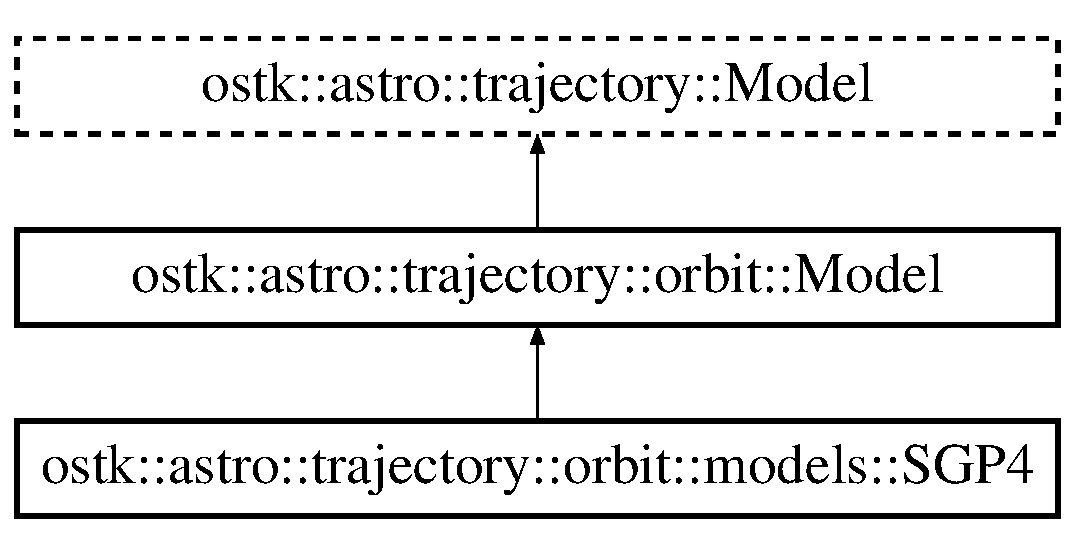
\includegraphics[height=3.000000cm]{classostk_1_1astro_1_1trajectory_1_1orbit_1_1models_1_1_s_g_p4}
\end{center}
\end{figure}
\doxysubsection*{Public Member Functions}
\begin{DoxyCompactItemize}
\item 
\mbox{\hyperlink{classostk_1_1astro_1_1trajectory_1_1orbit_1_1models_1_1_s_g_p4_a84e2bc60fdf9b295e0ab8a42ecfb51ff}{S\+G\+P4}} (const \mbox{\hyperlink{classostk_1_1astro_1_1trajectory_1_1orbit_1_1models_1_1sgp4_1_1_t_l_e}{T\+LE}} \&a\+Tle)
\item 
\mbox{\hyperlink{classostk_1_1astro_1_1trajectory_1_1orbit_1_1models_1_1_s_g_p4_afe0c5fa943d25263097c242c5b289239}{S\+G\+P4}} (const \mbox{\hyperlink{classostk_1_1astro_1_1trajectory_1_1orbit_1_1models_1_1_s_g_p4}{S\+G\+P4}} \&a\+S\+G\+P4\+Model)
\item 
\mbox{\hyperlink{classostk_1_1astro_1_1trajectory_1_1orbit_1_1models_1_1_s_g_p4_a00ac84881288a79f3c876efd56c376eb}{$\sim$\+S\+G\+P4}} ()
\item 
\mbox{\hyperlink{classostk_1_1astro_1_1trajectory_1_1orbit_1_1models_1_1_s_g_p4}{S\+G\+P4}} \& \mbox{\hyperlink{classostk_1_1astro_1_1trajectory_1_1orbit_1_1models_1_1_s_g_p4_a8f8d3633270de5c9d8c99f047f28d0f0}{operator=}} (const \mbox{\hyperlink{classostk_1_1astro_1_1trajectory_1_1orbit_1_1models_1_1_s_g_p4}{S\+G\+P4}} \&a\+S\+G\+P4\+Model)
\item 
virtual \mbox{\hyperlink{classostk_1_1astro_1_1trajectory_1_1orbit_1_1models_1_1_s_g_p4}{S\+G\+P4}} $\ast$ \mbox{\hyperlink{classostk_1_1astro_1_1trajectory_1_1orbit_1_1models_1_1_s_g_p4_afb9928e09d66c13a77eb1126da6139eb}{clone}} () const override
\item 
bool \mbox{\hyperlink{classostk_1_1astro_1_1trajectory_1_1orbit_1_1models_1_1_s_g_p4_ac95f88e801e75d53c2908cfc55d743a0}{operator==}} (const \mbox{\hyperlink{classostk_1_1astro_1_1trajectory_1_1orbit_1_1models_1_1_s_g_p4}{S\+G\+P4}} \&a\+S\+G\+P4\+Model) const
\item 
bool \mbox{\hyperlink{classostk_1_1astro_1_1trajectory_1_1orbit_1_1models_1_1_s_g_p4_a6daa973c340543e56c134cd2daf867f6}{operator!=}} (const \mbox{\hyperlink{classostk_1_1astro_1_1trajectory_1_1orbit_1_1models_1_1_s_g_p4}{S\+G\+P4}} \&a\+S\+G\+P4\+Model) const
\item 
virtual bool \mbox{\hyperlink{classostk_1_1astro_1_1trajectory_1_1orbit_1_1models_1_1_s_g_p4_ab18e0666588bd517c190942b1a54ed18}{is\+Defined}} () const override
\item 
\mbox{\hyperlink{classostk_1_1astro_1_1trajectory_1_1orbit_1_1models_1_1sgp4_1_1_t_l_e}{T\+LE}} \mbox{\hyperlink{classostk_1_1astro_1_1trajectory_1_1orbit_1_1models_1_1_s_g_p4_ac1f2188866759569091ebfd8e43919a8}{get\+Tle}} () const
\item 
virtual Instant \mbox{\hyperlink{classostk_1_1astro_1_1trajectory_1_1orbit_1_1models_1_1_s_g_p4_af577ee4ad56452fe510d325a61a9792e}{get\+Epoch}} () const override
\item 
virtual Integer \mbox{\hyperlink{classostk_1_1astro_1_1trajectory_1_1orbit_1_1models_1_1_s_g_p4_a6216f01c1ee37817ca1ae1c7036f942c}{get\+Revolution\+Number\+At\+Epoch}} () const override
\item 
virtual \mbox{\hyperlink{classostk_1_1astro_1_1trajectory_1_1_state}{State}} \mbox{\hyperlink{classostk_1_1astro_1_1trajectory_1_1orbit_1_1models_1_1_s_g_p4_ad88439d9c46a75d3da8c20d2872271e3}{calculate\+State\+At}} (const Instant \&an\+Instant) const override
\item 
virtual Integer \mbox{\hyperlink{classostk_1_1astro_1_1trajectory_1_1orbit_1_1models_1_1_s_g_p4_af14e7851024d96eb20033ca9296dc003}{calculate\+Revolution\+Number\+At}} (const Instant \&an\+Instant) const override
\item 
virtual void \mbox{\hyperlink{classostk_1_1astro_1_1trajectory_1_1orbit_1_1models_1_1_s_g_p4_a12416476201382c3d1e3c620f7be106a}{print}} (std\+::ostream \&an\+Output\+Stream, bool display\+Decorator=true) const override
\end{DoxyCompactItemize}
\doxysubsection*{Protected Member Functions}
\begin{DoxyCompactItemize}
\item 
virtual bool \mbox{\hyperlink{classostk_1_1astro_1_1trajectory_1_1orbit_1_1models_1_1_s_g_p4_ad51d979b8b9b37251b6381cfe9df55ea}{operator==}} (const \mbox{\hyperlink{classostk_1_1astro_1_1trajectory_1_1_model}{trajectory\+::\+Model}} \&a\+Model) const override
\item 
virtual bool \mbox{\hyperlink{classostk_1_1astro_1_1trajectory_1_1orbit_1_1models_1_1_s_g_p4_a87441104e4e1c63356abe0632b56edb6}{operator!=}} (const \mbox{\hyperlink{classostk_1_1astro_1_1trajectory_1_1_model}{trajectory\+::\+Model}} \&a\+Model) const override
\end{DoxyCompactItemize}
\doxysubsection*{Friends}
\begin{DoxyCompactItemize}
\item 
std\+::ostream \& \mbox{\hyperlink{classostk_1_1astro_1_1trajectory_1_1orbit_1_1models_1_1_s_g_p4_a44bd6a41f5d1be384d07b897785529f1}{operator$<$$<$}} (std\+::ostream \&an\+Output\+Stream, const \mbox{\hyperlink{classostk_1_1astro_1_1trajectory_1_1orbit_1_1models_1_1_s_g_p4}{S\+G\+P4}} \&a\+S\+G\+P4\+Model)
\end{DoxyCompactItemize}


\doxysubsection{Constructor \& Destructor Documentation}
\mbox{\Hypertarget{classostk_1_1astro_1_1trajectory_1_1orbit_1_1models_1_1_s_g_p4_a84e2bc60fdf9b295e0ab8a42ecfb51ff}\label{classostk_1_1astro_1_1trajectory_1_1orbit_1_1models_1_1_s_g_p4_a84e2bc60fdf9b295e0ab8a42ecfb51ff}} 
\index{ostk::astro::trajectory::orbit::models::SGP4@{ostk::astro::trajectory::orbit::models::SGP4}!SGP4@{SGP4}}
\index{SGP4@{SGP4}!ostk::astro::trajectory::orbit::models::SGP4@{ostk::astro::trajectory::orbit::models::SGP4}}
\doxysubsubsection{\texorpdfstring{SGP4()}{SGP4()}\hspace{0.1cm}{\footnotesize\ttfamily [1/2]}}
{\footnotesize\ttfamily ostk\+::astro\+::trajectory\+::orbit\+::models\+::\+S\+G\+P4\+::\+S\+G\+P4 (\begin{DoxyParamCaption}\item[{const \mbox{\hyperlink{classostk_1_1astro_1_1trajectory_1_1orbit_1_1models_1_1sgp4_1_1_t_l_e}{T\+LE}} \&}]{a\+Tle }\end{DoxyParamCaption})}

\mbox{\Hypertarget{classostk_1_1astro_1_1trajectory_1_1orbit_1_1models_1_1_s_g_p4_afe0c5fa943d25263097c242c5b289239}\label{classostk_1_1astro_1_1trajectory_1_1orbit_1_1models_1_1_s_g_p4_afe0c5fa943d25263097c242c5b289239}} 
\index{ostk::astro::trajectory::orbit::models::SGP4@{ostk::astro::trajectory::orbit::models::SGP4}!SGP4@{SGP4}}
\index{SGP4@{SGP4}!ostk::astro::trajectory::orbit::models::SGP4@{ostk::astro::trajectory::orbit::models::SGP4}}
\doxysubsubsection{\texorpdfstring{SGP4()}{SGP4()}\hspace{0.1cm}{\footnotesize\ttfamily [2/2]}}
{\footnotesize\ttfamily ostk\+::astro\+::trajectory\+::orbit\+::models\+::\+S\+G\+P4\+::\+S\+G\+P4 (\begin{DoxyParamCaption}\item[{const \mbox{\hyperlink{classostk_1_1astro_1_1trajectory_1_1orbit_1_1models_1_1_s_g_p4}{S\+G\+P4}} \&}]{a\+S\+G\+P4\+Model }\end{DoxyParamCaption})}

\mbox{\Hypertarget{classostk_1_1astro_1_1trajectory_1_1orbit_1_1models_1_1_s_g_p4_a00ac84881288a79f3c876efd56c376eb}\label{classostk_1_1astro_1_1trajectory_1_1orbit_1_1models_1_1_s_g_p4_a00ac84881288a79f3c876efd56c376eb}} 
\index{ostk::astro::trajectory::orbit::models::SGP4@{ostk::astro::trajectory::orbit::models::SGP4}!````~SGP4@{$\sim$SGP4}}
\index{````~SGP4@{$\sim$SGP4}!ostk::astro::trajectory::orbit::models::SGP4@{ostk::astro::trajectory::orbit::models::SGP4}}
\doxysubsubsection{\texorpdfstring{$\sim$SGP4()}{~SGP4()}}
{\footnotesize\ttfamily ostk\+::astro\+::trajectory\+::orbit\+::models\+::\+S\+G\+P4\+::$\sim$\+S\+G\+P4 (\begin{DoxyParamCaption}{ }\end{DoxyParamCaption})}



\doxysubsection{Member Function Documentation}
\mbox{\Hypertarget{classostk_1_1astro_1_1trajectory_1_1orbit_1_1models_1_1_s_g_p4_af14e7851024d96eb20033ca9296dc003}\label{classostk_1_1astro_1_1trajectory_1_1orbit_1_1models_1_1_s_g_p4_af14e7851024d96eb20033ca9296dc003}} 
\index{ostk::astro::trajectory::orbit::models::SGP4@{ostk::astro::trajectory::orbit::models::SGP4}!calculateRevolutionNumberAt@{calculateRevolutionNumberAt}}
\index{calculateRevolutionNumberAt@{calculateRevolutionNumberAt}!ostk::astro::trajectory::orbit::models::SGP4@{ostk::astro::trajectory::orbit::models::SGP4}}
\doxysubsubsection{\texorpdfstring{calculateRevolutionNumberAt()}{calculateRevolutionNumberAt()}}
{\footnotesize\ttfamily Integer ostk\+::astro\+::trajectory\+::orbit\+::models\+::\+S\+G\+P4\+::calculate\+Revolution\+Number\+At (\begin{DoxyParamCaption}\item[{const Instant \&}]{an\+Instant }\end{DoxyParamCaption}) const\hspace{0.3cm}{\ttfamily [override]}, {\ttfamily [virtual]}}



Implements \mbox{\hyperlink{classostk_1_1astro_1_1trajectory_1_1orbit_1_1_model_aeecf4cc22fa9c766801936c468cc52ac}{ostk\+::astro\+::trajectory\+::orbit\+::\+Model}}.

\mbox{\Hypertarget{classostk_1_1astro_1_1trajectory_1_1orbit_1_1models_1_1_s_g_p4_ad88439d9c46a75d3da8c20d2872271e3}\label{classostk_1_1astro_1_1trajectory_1_1orbit_1_1models_1_1_s_g_p4_ad88439d9c46a75d3da8c20d2872271e3}} 
\index{ostk::astro::trajectory::orbit::models::SGP4@{ostk::astro::trajectory::orbit::models::SGP4}!calculateStateAt@{calculateStateAt}}
\index{calculateStateAt@{calculateStateAt}!ostk::astro::trajectory::orbit::models::SGP4@{ostk::astro::trajectory::orbit::models::SGP4}}
\doxysubsubsection{\texorpdfstring{calculateStateAt()}{calculateStateAt()}}
{\footnotesize\ttfamily \mbox{\hyperlink{classostk_1_1astro_1_1trajectory_1_1_state}{State}} ostk\+::astro\+::trajectory\+::orbit\+::models\+::\+S\+G\+P4\+::calculate\+State\+At (\begin{DoxyParamCaption}\item[{const Instant \&}]{an\+Instant }\end{DoxyParamCaption}) const\hspace{0.3cm}{\ttfamily [override]}, {\ttfamily [virtual]}}



Implements \mbox{\hyperlink{classostk_1_1astro_1_1trajectory_1_1orbit_1_1_model_a34a0d8979ec1f7ade3e434fc0dad3711}{ostk\+::astro\+::trajectory\+::orbit\+::\+Model}}.

\mbox{\Hypertarget{classostk_1_1astro_1_1trajectory_1_1orbit_1_1models_1_1_s_g_p4_afb9928e09d66c13a77eb1126da6139eb}\label{classostk_1_1astro_1_1trajectory_1_1orbit_1_1models_1_1_s_g_p4_afb9928e09d66c13a77eb1126da6139eb}} 
\index{ostk::astro::trajectory::orbit::models::SGP4@{ostk::astro::trajectory::orbit::models::SGP4}!clone@{clone}}
\index{clone@{clone}!ostk::astro::trajectory::orbit::models::SGP4@{ostk::astro::trajectory::orbit::models::SGP4}}
\doxysubsubsection{\texorpdfstring{clone()}{clone()}}
{\footnotesize\ttfamily \mbox{\hyperlink{classostk_1_1astro_1_1trajectory_1_1orbit_1_1models_1_1_s_g_p4}{S\+G\+P4}} $\ast$ ostk\+::astro\+::trajectory\+::orbit\+::models\+::\+S\+G\+P4\+::clone (\begin{DoxyParamCaption}{ }\end{DoxyParamCaption}) const\hspace{0.3cm}{\ttfamily [override]}, {\ttfamily [virtual]}}



Implements \mbox{\hyperlink{classostk_1_1astro_1_1trajectory_1_1orbit_1_1_model_a53dc07564e4c7c444da46360aa8ada15}{ostk\+::astro\+::trajectory\+::orbit\+::\+Model}}.

\mbox{\Hypertarget{classostk_1_1astro_1_1trajectory_1_1orbit_1_1models_1_1_s_g_p4_af577ee4ad56452fe510d325a61a9792e}\label{classostk_1_1astro_1_1trajectory_1_1orbit_1_1models_1_1_s_g_p4_af577ee4ad56452fe510d325a61a9792e}} 
\index{ostk::astro::trajectory::orbit::models::SGP4@{ostk::astro::trajectory::orbit::models::SGP4}!getEpoch@{getEpoch}}
\index{getEpoch@{getEpoch}!ostk::astro::trajectory::orbit::models::SGP4@{ostk::astro::trajectory::orbit::models::SGP4}}
\doxysubsubsection{\texorpdfstring{getEpoch()}{getEpoch()}}
{\footnotesize\ttfamily Instant ostk\+::astro\+::trajectory\+::orbit\+::models\+::\+S\+G\+P4\+::get\+Epoch (\begin{DoxyParamCaption}{ }\end{DoxyParamCaption}) const\hspace{0.3cm}{\ttfamily [override]}, {\ttfamily [virtual]}}



Implements \mbox{\hyperlink{classostk_1_1astro_1_1trajectory_1_1orbit_1_1_model_a22055d5ab4c22e6177a3ddb8f45f1f9b}{ostk\+::astro\+::trajectory\+::orbit\+::\+Model}}.

\mbox{\Hypertarget{classostk_1_1astro_1_1trajectory_1_1orbit_1_1models_1_1_s_g_p4_a6216f01c1ee37817ca1ae1c7036f942c}\label{classostk_1_1astro_1_1trajectory_1_1orbit_1_1models_1_1_s_g_p4_a6216f01c1ee37817ca1ae1c7036f942c}} 
\index{ostk::astro::trajectory::orbit::models::SGP4@{ostk::astro::trajectory::orbit::models::SGP4}!getRevolutionNumberAtEpoch@{getRevolutionNumberAtEpoch}}
\index{getRevolutionNumberAtEpoch@{getRevolutionNumberAtEpoch}!ostk::astro::trajectory::orbit::models::SGP4@{ostk::astro::trajectory::orbit::models::SGP4}}
\doxysubsubsection{\texorpdfstring{getRevolutionNumberAtEpoch()}{getRevolutionNumberAtEpoch()}}
{\footnotesize\ttfamily Integer ostk\+::astro\+::trajectory\+::orbit\+::models\+::\+S\+G\+P4\+::get\+Revolution\+Number\+At\+Epoch (\begin{DoxyParamCaption}{ }\end{DoxyParamCaption}) const\hspace{0.3cm}{\ttfamily [override]}, {\ttfamily [virtual]}}



Implements \mbox{\hyperlink{classostk_1_1astro_1_1trajectory_1_1orbit_1_1_model_af3f1866f86045da2c05efe4165735cf4}{ostk\+::astro\+::trajectory\+::orbit\+::\+Model}}.

\mbox{\Hypertarget{classostk_1_1astro_1_1trajectory_1_1orbit_1_1models_1_1_s_g_p4_ac1f2188866759569091ebfd8e43919a8}\label{classostk_1_1astro_1_1trajectory_1_1orbit_1_1models_1_1_s_g_p4_ac1f2188866759569091ebfd8e43919a8}} 
\index{ostk::astro::trajectory::orbit::models::SGP4@{ostk::astro::trajectory::orbit::models::SGP4}!getTle@{getTle}}
\index{getTle@{getTle}!ostk::astro::trajectory::orbit::models::SGP4@{ostk::astro::trajectory::orbit::models::SGP4}}
\doxysubsubsection{\texorpdfstring{getTle()}{getTle()}}
{\footnotesize\ttfamily \mbox{\hyperlink{classostk_1_1astro_1_1trajectory_1_1orbit_1_1models_1_1sgp4_1_1_t_l_e}{T\+LE}} ostk\+::astro\+::trajectory\+::orbit\+::models\+::\+S\+G\+P4\+::get\+Tle (\begin{DoxyParamCaption}{ }\end{DoxyParamCaption}) const}

\mbox{\Hypertarget{classostk_1_1astro_1_1trajectory_1_1orbit_1_1models_1_1_s_g_p4_ab18e0666588bd517c190942b1a54ed18}\label{classostk_1_1astro_1_1trajectory_1_1orbit_1_1models_1_1_s_g_p4_ab18e0666588bd517c190942b1a54ed18}} 
\index{ostk::astro::trajectory::orbit::models::SGP4@{ostk::astro::trajectory::orbit::models::SGP4}!isDefined@{isDefined}}
\index{isDefined@{isDefined}!ostk::astro::trajectory::orbit::models::SGP4@{ostk::astro::trajectory::orbit::models::SGP4}}
\doxysubsubsection{\texorpdfstring{isDefined()}{isDefined()}}
{\footnotesize\ttfamily bool ostk\+::astro\+::trajectory\+::orbit\+::models\+::\+S\+G\+P4\+::is\+Defined (\begin{DoxyParamCaption}{ }\end{DoxyParamCaption}) const\hspace{0.3cm}{\ttfamily [override]}, {\ttfamily [virtual]}}



Implements \mbox{\hyperlink{classostk_1_1astro_1_1trajectory_1_1orbit_1_1_model_a13c5b5693dd86a072da0bd0e319bacc2}{ostk\+::astro\+::trajectory\+::orbit\+::\+Model}}.

\mbox{\Hypertarget{classostk_1_1astro_1_1trajectory_1_1orbit_1_1models_1_1_s_g_p4_a6daa973c340543e56c134cd2daf867f6}\label{classostk_1_1astro_1_1trajectory_1_1orbit_1_1models_1_1_s_g_p4_a6daa973c340543e56c134cd2daf867f6}} 
\index{ostk::astro::trajectory::orbit::models::SGP4@{ostk::astro::trajectory::orbit::models::SGP4}!operator"!=@{operator"!=}}
\index{operator"!=@{operator"!=}!ostk::astro::trajectory::orbit::models::SGP4@{ostk::astro::trajectory::orbit::models::SGP4}}
\doxysubsubsection{\texorpdfstring{operator"!=()}{operator!=()}\hspace{0.1cm}{\footnotesize\ttfamily [1/2]}}
{\footnotesize\ttfamily bool ostk\+::astro\+::trajectory\+::orbit\+::models\+::\+S\+G\+P4\+::operator!= (\begin{DoxyParamCaption}\item[{const \mbox{\hyperlink{classostk_1_1astro_1_1trajectory_1_1orbit_1_1models_1_1_s_g_p4}{S\+G\+P4}} \&}]{a\+S\+G\+P4\+Model }\end{DoxyParamCaption}) const}

\mbox{\Hypertarget{classostk_1_1astro_1_1trajectory_1_1orbit_1_1models_1_1_s_g_p4_a87441104e4e1c63356abe0632b56edb6}\label{classostk_1_1astro_1_1trajectory_1_1orbit_1_1models_1_1_s_g_p4_a87441104e4e1c63356abe0632b56edb6}} 
\index{ostk::astro::trajectory::orbit::models::SGP4@{ostk::astro::trajectory::orbit::models::SGP4}!operator"!=@{operator"!=}}
\index{operator"!=@{operator"!=}!ostk::astro::trajectory::orbit::models::SGP4@{ostk::astro::trajectory::orbit::models::SGP4}}
\doxysubsubsection{\texorpdfstring{operator"!=()}{operator!=()}\hspace{0.1cm}{\footnotesize\ttfamily [2/2]}}
{\footnotesize\ttfamily bool ostk\+::astro\+::trajectory\+::orbit\+::models\+::\+S\+G\+P4\+::operator!= (\begin{DoxyParamCaption}\item[{const \mbox{\hyperlink{classostk_1_1astro_1_1trajectory_1_1_model}{trajectory\+::\+Model}} \&}]{a\+Model }\end{DoxyParamCaption}) const\hspace{0.3cm}{\ttfamily [override]}, {\ttfamily [protected]}, {\ttfamily [virtual]}}



Implements \mbox{\hyperlink{classostk_1_1astro_1_1trajectory_1_1_model_a2dd77b9f6939d738f3a489f26c955340}{ostk\+::astro\+::trajectory\+::\+Model}}.

\mbox{\Hypertarget{classostk_1_1astro_1_1trajectory_1_1orbit_1_1models_1_1_s_g_p4_a8f8d3633270de5c9d8c99f047f28d0f0}\label{classostk_1_1astro_1_1trajectory_1_1orbit_1_1models_1_1_s_g_p4_a8f8d3633270de5c9d8c99f047f28d0f0}} 
\index{ostk::astro::trajectory::orbit::models::SGP4@{ostk::astro::trajectory::orbit::models::SGP4}!operator=@{operator=}}
\index{operator=@{operator=}!ostk::astro::trajectory::orbit::models::SGP4@{ostk::astro::trajectory::orbit::models::SGP4}}
\doxysubsubsection{\texorpdfstring{operator=()}{operator=()}}
{\footnotesize\ttfamily \mbox{\hyperlink{classostk_1_1astro_1_1trajectory_1_1orbit_1_1models_1_1_s_g_p4}{S\+G\+P4}} \& ostk\+::astro\+::trajectory\+::orbit\+::models\+::\+S\+G\+P4\+::operator= (\begin{DoxyParamCaption}\item[{const \mbox{\hyperlink{classostk_1_1astro_1_1trajectory_1_1orbit_1_1models_1_1_s_g_p4}{S\+G\+P4}} \&}]{a\+S\+G\+P4\+Model }\end{DoxyParamCaption})}

\mbox{\Hypertarget{classostk_1_1astro_1_1trajectory_1_1orbit_1_1models_1_1_s_g_p4_ac95f88e801e75d53c2908cfc55d743a0}\label{classostk_1_1astro_1_1trajectory_1_1orbit_1_1models_1_1_s_g_p4_ac95f88e801e75d53c2908cfc55d743a0}} 
\index{ostk::astro::trajectory::orbit::models::SGP4@{ostk::astro::trajectory::orbit::models::SGP4}!operator==@{operator==}}
\index{operator==@{operator==}!ostk::astro::trajectory::orbit::models::SGP4@{ostk::astro::trajectory::orbit::models::SGP4}}
\doxysubsubsection{\texorpdfstring{operator==()}{operator==()}\hspace{0.1cm}{\footnotesize\ttfamily [1/2]}}
{\footnotesize\ttfamily bool ostk\+::astro\+::trajectory\+::orbit\+::models\+::\+S\+G\+P4\+::operator== (\begin{DoxyParamCaption}\item[{const \mbox{\hyperlink{classostk_1_1astro_1_1trajectory_1_1orbit_1_1models_1_1_s_g_p4}{S\+G\+P4}} \&}]{a\+S\+G\+P4\+Model }\end{DoxyParamCaption}) const}

\mbox{\Hypertarget{classostk_1_1astro_1_1trajectory_1_1orbit_1_1models_1_1_s_g_p4_ad51d979b8b9b37251b6381cfe9df55ea}\label{classostk_1_1astro_1_1trajectory_1_1orbit_1_1models_1_1_s_g_p4_ad51d979b8b9b37251b6381cfe9df55ea}} 
\index{ostk::astro::trajectory::orbit::models::SGP4@{ostk::astro::trajectory::orbit::models::SGP4}!operator==@{operator==}}
\index{operator==@{operator==}!ostk::astro::trajectory::orbit::models::SGP4@{ostk::astro::trajectory::orbit::models::SGP4}}
\doxysubsubsection{\texorpdfstring{operator==()}{operator==()}\hspace{0.1cm}{\footnotesize\ttfamily [2/2]}}
{\footnotesize\ttfamily bool ostk\+::astro\+::trajectory\+::orbit\+::models\+::\+S\+G\+P4\+::operator== (\begin{DoxyParamCaption}\item[{const \mbox{\hyperlink{classostk_1_1astro_1_1trajectory_1_1_model}{trajectory\+::\+Model}} \&}]{a\+Model }\end{DoxyParamCaption}) const\hspace{0.3cm}{\ttfamily [override]}, {\ttfamily [protected]}, {\ttfamily [virtual]}}



Implements \mbox{\hyperlink{classostk_1_1astro_1_1trajectory_1_1_model_a874f79846e845859c070ce1b9874fc9c}{ostk\+::astro\+::trajectory\+::\+Model}}.

\mbox{\Hypertarget{classostk_1_1astro_1_1trajectory_1_1orbit_1_1models_1_1_s_g_p4_a12416476201382c3d1e3c620f7be106a}\label{classostk_1_1astro_1_1trajectory_1_1orbit_1_1models_1_1_s_g_p4_a12416476201382c3d1e3c620f7be106a}} 
\index{ostk::astro::trajectory::orbit::models::SGP4@{ostk::astro::trajectory::orbit::models::SGP4}!print@{print}}
\index{print@{print}!ostk::astro::trajectory::orbit::models::SGP4@{ostk::astro::trajectory::orbit::models::SGP4}}
\doxysubsubsection{\texorpdfstring{print()}{print()}}
{\footnotesize\ttfamily void ostk\+::astro\+::trajectory\+::orbit\+::models\+::\+S\+G\+P4\+::print (\begin{DoxyParamCaption}\item[{std\+::ostream \&}]{an\+Output\+Stream,  }\item[{bool}]{display\+Decorator = {\ttfamily true} }\end{DoxyParamCaption}) const\hspace{0.3cm}{\ttfamily [override]}, {\ttfamily [virtual]}}



Implements \mbox{\hyperlink{classostk_1_1astro_1_1trajectory_1_1orbit_1_1_model_a8ea45c1a6e51a6153ce3f72f5294f0c6}{ostk\+::astro\+::trajectory\+::orbit\+::\+Model}}.



\doxysubsection{Friends And Related Function Documentation}
\mbox{\Hypertarget{classostk_1_1astro_1_1trajectory_1_1orbit_1_1models_1_1_s_g_p4_a44bd6a41f5d1be384d07b897785529f1}\label{classostk_1_1astro_1_1trajectory_1_1orbit_1_1models_1_1_s_g_p4_a44bd6a41f5d1be384d07b897785529f1}} 
\index{ostk::astro::trajectory::orbit::models::SGP4@{ostk::astro::trajectory::orbit::models::SGP4}!operator$<$$<$@{operator$<$$<$}}
\index{operator$<$$<$@{operator$<$$<$}!ostk::astro::trajectory::orbit::models::SGP4@{ostk::astro::trajectory::orbit::models::SGP4}}
\doxysubsubsection{\texorpdfstring{operator$<$$<$}{operator<<}}
{\footnotesize\ttfamily std\+::ostream\& operator$<$$<$ (\begin{DoxyParamCaption}\item[{std\+::ostream \&}]{an\+Output\+Stream,  }\item[{const \mbox{\hyperlink{classostk_1_1astro_1_1trajectory_1_1orbit_1_1models_1_1_s_g_p4}{S\+G\+P4}} \&}]{a\+S\+G\+P4\+Model }\end{DoxyParamCaption})\hspace{0.3cm}{\ttfamily [friend]}}



The documentation for this class was generated from the following files\+:\begin{DoxyCompactItemize}
\item 
include/\+Open\+Space\+Toolkit/\+Astrodynamics/\+Trajectory/\+Orbit/\+Models/\mbox{\hyperlink{_s_g_p4_8hpp}{S\+G\+P4.\+hpp}}\item 
src/\+Open\+Space\+Toolkit/\+Astrodynamics/\+Trajectory/\+Orbit/\+Models/\mbox{\hyperlink{_s_g_p4_8cpp}{S\+G\+P4.\+cpp}}\end{DoxyCompactItemize}

\hypertarget{classostk_1_1astro_1_1trajectory_1_1_state}{}\doxysection{ostk\+::astro\+::trajectory\+::State Class Reference}
\label{classostk_1_1astro_1_1trajectory_1_1_state}\index{ostk::astro::trajectory::State@{ostk::astro::trajectory::State}}


\mbox{\hyperlink{classostk_1_1astro_1_1_trajectory}{Trajectory}} \mbox{\hyperlink{classostk_1_1astro_1_1trajectory_1_1_state}{State}}.  




{\ttfamily \#include $<$State.\+hpp$>$}

\doxysubsection*{Public Member Functions}
\begin{DoxyCompactItemize}
\item 
\mbox{\hyperlink{classostk_1_1astro_1_1trajectory_1_1_state_abbaa96f2d2b7f388eb073daab94202b3}{State}} (const Instant \&an\+Instant, const Vector\+Xd \&a\+Coordinates, const Shared$<$ const Frame $>$ \&a\+Frame\+S\+Ptr, const Shared$<$ const \mbox{\hyperlink{classostk_1_1astro_1_1trajectory_1_1state_1_1_coordinates_broker}{Coordinates\+Broker}} $>$ \&a\+Coordinates\+Broker\+S\+Ptr)
\begin{DoxyCompactList}\small\item\em Constructor with a pre-\/defined Coordinates Broker. \end{DoxyCompactList}\item 
\mbox{\hyperlink{classostk_1_1astro_1_1trajectory_1_1_state_a9774b1ddfacd2707986066f5f0650368}{State}} (const Instant \&an\+Instant, const Vector\+Xd \&a\+Coordinates, const Shared$<$ const Frame $>$ \&a\+Frame\+S\+Ptr, const Array$<$ Shared$<$ const \mbox{\hyperlink{classostk_1_1astro_1_1trajectory_1_1state_1_1_coordinates_subset}{Coordinates\+Subset}} $>$$>$ \&a\+Coordinates\+Subsets\+Array)
\begin{DoxyCompactList}\small\item\em Constructor. This constructor makes a new Coordinates Broker under the hood for every \mbox{\hyperlink{classostk_1_1astro_1_1trajectory_1_1_state}{State}}. When possible, users should prefer passing in an existing Coordinates Broker or using a \mbox{\hyperlink{classostk_1_1astro_1_1trajectory_1_1_state_builder}{State\+Builder}} to reduce memory footprint when constructing many states. \end{DoxyCompactList}\item 
\mbox{\hyperlink{classostk_1_1astro_1_1trajectory_1_1_state_a01ef71cfac563cfbc8b5082ccd379227}{State}} (const Instant \&an\+Instant, const Position \&a\+Position, const Velocity \&a\+Velocity, const Quaternion \&an\+Attitude, const Vector3d \&an\+Angular\+Velocity, const Shared$<$ const Frame $>$ \&an\+Attitude\+Reference\+Frame)
\begin{DoxyCompactList}\small\item\em Utility constructor for Position/\+Velocity/\+Attitude/\+Angular Velocity. \end{DoxyCompactList}\item 
\mbox{\hyperlink{classostk_1_1astro_1_1trajectory_1_1_state_a8628aceae903c9492f0fb269888434b0}{State}} (const Instant \&an\+Instant, const Position \&a\+Position, const Velocity \&a\+Velocity)
\begin{DoxyCompactList}\small\item\em Utility constructor for Position/\+Velocity only. \end{DoxyCompactList}\item 
\mbox{\hyperlink{classostk_1_1astro_1_1trajectory_1_1_state_ac8657234876a3e043bcdfa7f88470e77}{State}} (const \mbox{\hyperlink{classostk_1_1astro_1_1trajectory_1_1_state}{State}} \&a\+State)
\begin{DoxyCompactList}\small\item\em Copy constructor. \end{DoxyCompactList}\item 
\mbox{\hyperlink{classostk_1_1astro_1_1trajectory_1_1_state}{State}} \& \mbox{\hyperlink{classostk_1_1astro_1_1trajectory_1_1_state_ac4281382f859c517dd6233f341cdac66}{operator=}} (const \mbox{\hyperlink{classostk_1_1astro_1_1trajectory_1_1_state}{State}} \&a\+State)
\begin{DoxyCompactList}\small\item\em Copy-\/assignment operator. \end{DoxyCompactList}\item 
bool \mbox{\hyperlink{classostk_1_1astro_1_1trajectory_1_1_state_acd68798b63a7e3a89e61b4b668d8dbb0}{operator==}} (const \mbox{\hyperlink{classostk_1_1astro_1_1trajectory_1_1_state}{State}} \&a\+State) const
\begin{DoxyCompactList}\small\item\em Equality operator. \end{DoxyCompactList}\item 
bool \mbox{\hyperlink{classostk_1_1astro_1_1trajectory_1_1_state_a53ac2b13092bc7777efa14362fec4c46}{operator!=}} (const \mbox{\hyperlink{classostk_1_1astro_1_1trajectory_1_1_state}{State}} \&a\+State) const
\begin{DoxyCompactList}\small\item\em Inequality operator. \end{DoxyCompactList}\item 
\mbox{\hyperlink{classostk_1_1astro_1_1trajectory_1_1_state}{State}} \mbox{\hyperlink{classostk_1_1astro_1_1trajectory_1_1_state_a8d8ff34816c5e4895f9274fc06dbb799}{operator+}} (const \mbox{\hyperlink{classostk_1_1astro_1_1trajectory_1_1_state}{State}} \&a\+State) const
\begin{DoxyCompactList}\small\item\em Addition operator. \end{DoxyCompactList}\item 
\mbox{\hyperlink{classostk_1_1astro_1_1trajectory_1_1_state}{State}} \mbox{\hyperlink{classostk_1_1astro_1_1trajectory_1_1_state_abd0979467d66ca07b86d5405255d26ed}{operator-\/}} (const \mbox{\hyperlink{classostk_1_1astro_1_1trajectory_1_1_state}{State}} \&a\+State) const
\begin{DoxyCompactList}\small\item\em Subtraction operator. \end{DoxyCompactList}\item 
bool \mbox{\hyperlink{classostk_1_1astro_1_1trajectory_1_1_state_a09966efb00e3206cc2d20935c55658ad}{is\+Defined}} () const
\begin{DoxyCompactList}\small\item\em Check if the \mbox{\hyperlink{classostk_1_1astro_1_1trajectory_1_1_state}{State}} is defined. \end{DoxyCompactList}\item 
const Instant \& \mbox{\hyperlink{classostk_1_1astro_1_1trajectory_1_1_state_afc21870411eef52ce1293e31eda16d3c}{access\+Instant}} () const
\begin{DoxyCompactList}\small\item\em Accessor for the instant. \end{DoxyCompactList}\item 
const Shared$<$ const Frame $>$ \mbox{\hyperlink{classostk_1_1astro_1_1trajectory_1_1_state_a2490cdc545c5bb4d23bd14e8eb267f9e}{access\+Frame}} () const
\begin{DoxyCompactList}\small\item\em Accessor for the reference frame. \end{DoxyCompactList}\item 
const Vector\+Xd \& \mbox{\hyperlink{classostk_1_1astro_1_1trajectory_1_1_state_ae5823b96deced6c95a02eb35b56c396f}{access\+Coordinates}} () const
\begin{DoxyCompactList}\small\item\em Accessor for the coordinates. \end{DoxyCompactList}\item 
const Shared$<$ const \mbox{\hyperlink{classostk_1_1astro_1_1trajectory_1_1state_1_1_coordinates_broker}{Coordinates\+Broker}} $>$ \& \mbox{\hyperlink{classostk_1_1astro_1_1trajectory_1_1_state_af7aeabb36f72d0a2a9911176d4fe4f7f}{access\+Coordinates\+Broker}} () const
\begin{DoxyCompactList}\small\item\em \mbox{\hyperlink{classostk_1_1astro_1_1_access}{Access}} the coordinates broker associated with the \mbox{\hyperlink{classostk_1_1astro_1_1trajectory_1_1_state}{State}}. \end{DoxyCompactList}\item 
Size \mbox{\hyperlink{classostk_1_1astro_1_1trajectory_1_1_state_a858558cb5107a76d43c33a2f7d3ffaf6}{get\+Size}} () const
\begin{DoxyCompactList}\small\item\em Get the size of the \mbox{\hyperlink{classostk_1_1astro_1_1trajectory_1_1_state}{State}}. \end{DoxyCompactList}\item 
Instant \mbox{\hyperlink{classostk_1_1astro_1_1trajectory_1_1_state_af1ba3040b895b0963d5fb96a0756cc2b}{get\+Instant}} () const
\begin{DoxyCompactList}\small\item\em Get the instant associated with the \mbox{\hyperlink{classostk_1_1astro_1_1trajectory_1_1_state}{State}}. \end{DoxyCompactList}\item 
Shared$<$ const Frame $>$ \mbox{\hyperlink{classostk_1_1astro_1_1trajectory_1_1_state_a73f836fe73cf4a2829a2151ddac47477}{get\+Frame}} () const
\begin{DoxyCompactList}\small\item\em Get the reference frame associated with the \mbox{\hyperlink{classostk_1_1astro_1_1trajectory_1_1_state}{State}}. \end{DoxyCompactList}\item 
Position \mbox{\hyperlink{classostk_1_1astro_1_1trajectory_1_1_state_ad5ceac322a929f0f62214a663a21f4ae}{get\+Position}} () const
\begin{DoxyCompactList}\small\item\em Get the coordinates of the \mbox{\hyperlink{classostk_1_1astro_1_1trajectory_1_1_state}{State}}. \end{DoxyCompactList}\item 
Velocity \mbox{\hyperlink{classostk_1_1astro_1_1trajectory_1_1_state_a1a992dcad42fb3094766907a9472e7e0}{get\+Velocity}} () const
\begin{DoxyCompactList}\small\item\em Get the cartesian velocity associated with the \mbox{\hyperlink{classostk_1_1astro_1_1trajectory_1_1_state}{State}} (if present). \end{DoxyCompactList}\item 
Quaternion \mbox{\hyperlink{classostk_1_1astro_1_1trajectory_1_1_state_a715f423e24053bee743631bd1ded8af2}{get\+Attitude}} () const
\begin{DoxyCompactList}\small\item\em Get the attitude quaternion associated with the \mbox{\hyperlink{classostk_1_1astro_1_1trajectory_1_1_state}{State}} (if present). \end{DoxyCompactList}\item 
Vector3d \mbox{\hyperlink{classostk_1_1astro_1_1trajectory_1_1_state_a0220561e712152e60371d7ce203d50ca}{get\+Angular\+Velocity}} () const
\begin{DoxyCompactList}\small\item\em Get the angular velocity associated with the \mbox{\hyperlink{classostk_1_1astro_1_1trajectory_1_1_state}{State}} (if present). \end{DoxyCompactList}\item 
Vector\+Xd \mbox{\hyperlink{classostk_1_1astro_1_1trajectory_1_1_state_adece3f2dda107d9178b40648dfbc01d0}{get\+Coordinates}} () const
\begin{DoxyCompactList}\small\item\em Get the coordinates of the \mbox{\hyperlink{classostk_1_1astro_1_1trajectory_1_1_state}{State}}. \end{DoxyCompactList}\item 
const Array$<$ Shared$<$ const \mbox{\hyperlink{classostk_1_1astro_1_1trajectory_1_1state_1_1_coordinates_subset}{Coordinates\+Subset}} $>$ $>$ \mbox{\hyperlink{classostk_1_1astro_1_1trajectory_1_1_state_ad03f40490dd2a2572284221008be05f5}{get\+Coordinates\+Subsets}} () const
\begin{DoxyCompactList}\small\item\em Get the coordinates subsets of the \mbox{\hyperlink{classostk_1_1astro_1_1trajectory_1_1_state}{State}}. \end{DoxyCompactList}\item 
bool \mbox{\hyperlink{classostk_1_1astro_1_1trajectory_1_1_state_a03752b6712854c8369824408bab72e3c}{has\+Subset}} (const Shared$<$ const \mbox{\hyperlink{classostk_1_1astro_1_1trajectory_1_1state_1_1_coordinates_subset}{Coordinates\+Subset}} $>$ \&a\+Coordinates\+Subset\+S\+Ptr) const
\begin{DoxyCompactList}\small\item\em Check if the \mbox{\hyperlink{classostk_1_1astro_1_1trajectory_1_1_state}{State}} has a given coordinates subset. \end{DoxyCompactList}\item 
Vector\+Xd \mbox{\hyperlink{classostk_1_1astro_1_1trajectory_1_1_state_ae2681f516262a1f851fa91c57c3577cc}{extract\+Coordinate}} (const Shared$<$ const \mbox{\hyperlink{classostk_1_1astro_1_1trajectory_1_1state_1_1_coordinates_subset}{Coordinates\+Subset}} $>$ \&a\+Subset\+S\+Ptr) const
\begin{DoxyCompactList}\small\item\em Extract the coordinates for a single subset. \end{DoxyCompactList}\item 
Vector\+Xd \mbox{\hyperlink{classostk_1_1astro_1_1trajectory_1_1_state_aad1f1b9eeb7118bbe356520d3fe40f03}{extract\+Coordinates}} (const Array$<$ Shared$<$ const \mbox{\hyperlink{classostk_1_1astro_1_1trajectory_1_1state_1_1_coordinates_subset}{Coordinates\+Subset}} $>$$>$ \&a\+Coordinates\+Subsets\+Array) const
\begin{DoxyCompactList}\small\item\em Extract the coordinates for multiple subsets. \end{DoxyCompactList}\item 
\mbox{\hyperlink{classostk_1_1astro_1_1trajectory_1_1_state}{State}} \mbox{\hyperlink{classostk_1_1astro_1_1trajectory_1_1_state_aa9c95303df830f9dfed347231961dcf6}{in\+Frame}} (const Shared$<$ const Frame $>$ \&a\+Frame\+S\+Ptr) const
\begin{DoxyCompactList}\small\item\em Transform the \mbox{\hyperlink{classostk_1_1astro_1_1trajectory_1_1_state}{State}} to a different reference frame. \end{DoxyCompactList}\item 
void \mbox{\hyperlink{classostk_1_1astro_1_1trajectory_1_1_state_a0072b543bbac1abe5e94609c74491b5d}{print}} (std\+::ostream \&an\+Output\+Stream, bool display\+Decorator=true) const
\begin{DoxyCompactList}\small\item\em Print the \mbox{\hyperlink{classostk_1_1astro_1_1trajectory_1_1_state}{State}} to an output stream. \end{DoxyCompactList}\end{DoxyCompactItemize}
\doxysubsection*{Static Public Member Functions}
\begin{DoxyCompactItemize}
\item 
static \mbox{\hyperlink{classostk_1_1astro_1_1trajectory_1_1_state}{State}} \mbox{\hyperlink{classostk_1_1astro_1_1trajectory_1_1_state_ab6ed6a252eeac1d24cf3b5c65ec0c6b6}{Undefined}} ()
\begin{DoxyCompactList}\small\item\em Get an undefined \mbox{\hyperlink{classostk_1_1astro_1_1trajectory_1_1_state}{State}}. \end{DoxyCompactList}\end{DoxyCompactItemize}
\doxysubsection*{Friends}
\begin{DoxyCompactItemize}
\item 
std\+::ostream \& \mbox{\hyperlink{classostk_1_1astro_1_1trajectory_1_1_state_abba03f039f2534d691a1dc28426e8b89}{operator$<$$<$}} (std\+::ostream \&an\+Output\+Stream, const \mbox{\hyperlink{classostk_1_1astro_1_1trajectory_1_1_state}{State}} \&a\+State)
\begin{DoxyCompactList}\small\item\em Stream insertion operator. \end{DoxyCompactList}\end{DoxyCompactItemize}


\doxysubsection{Detailed Description}
\mbox{\hyperlink{classostk_1_1astro_1_1_trajectory}{Trajectory}} \mbox{\hyperlink{classostk_1_1astro_1_1trajectory_1_1_state}{State}}. 

\doxysubsection{Constructor \& Destructor Documentation}
\mbox{\Hypertarget{classostk_1_1astro_1_1trajectory_1_1_state_abbaa96f2d2b7f388eb073daab94202b3}\label{classostk_1_1astro_1_1trajectory_1_1_state_abbaa96f2d2b7f388eb073daab94202b3}} 
\index{ostk::astro::trajectory::State@{ostk::astro::trajectory::State}!State@{State}}
\index{State@{State}!ostk::astro::trajectory::State@{ostk::astro::trajectory::State}}
\doxysubsubsection{\texorpdfstring{State()}{State()}\hspace{0.1cm}{\footnotesize\ttfamily [1/5]}}
{\footnotesize\ttfamily ostk\+::astro\+::trajectory\+::\+State\+::\+State (\begin{DoxyParamCaption}\item[{const Instant \&}]{an\+Instant,  }\item[{const Vector\+Xd \&}]{a\+Coordinates,  }\item[{const Shared$<$ const Frame $>$ \&}]{a\+Frame\+S\+Ptr,  }\item[{const Shared$<$ const \mbox{\hyperlink{classostk_1_1astro_1_1trajectory_1_1state_1_1_coordinates_broker}{Coordinates\+Broker}} $>$ \&}]{a\+Coordinates\+Broker\+S\+Ptr }\end{DoxyParamCaption})}



Constructor with a pre-\/defined Coordinates Broker. 


\begin{DoxyParams}{Parameters}
{\em an\+Instant} & An instant \\
\hline
{\em a\+Coordinates} & The coordinates at the instant in International System of Units \\
\hline
{\em a\+Frame\+S\+Ptr} & The reference frame in which the coordinates are referenced to and resolved in \\
\hline
{\em a\+Coordinates\+Broker\+S\+Ptr} & The coordinates broker associated to the coordinates \\
\hline
\end{DoxyParams}
\mbox{\Hypertarget{classostk_1_1astro_1_1trajectory_1_1_state_a9774b1ddfacd2707986066f5f0650368}\label{classostk_1_1astro_1_1trajectory_1_1_state_a9774b1ddfacd2707986066f5f0650368}} 
\index{ostk::astro::trajectory::State@{ostk::astro::trajectory::State}!State@{State}}
\index{State@{State}!ostk::astro::trajectory::State@{ostk::astro::trajectory::State}}
\doxysubsubsection{\texorpdfstring{State()}{State()}\hspace{0.1cm}{\footnotesize\ttfamily [2/5]}}
{\footnotesize\ttfamily ostk\+::astro\+::trajectory\+::\+State\+::\+State (\begin{DoxyParamCaption}\item[{const Instant \&}]{an\+Instant,  }\item[{const Vector\+Xd \&}]{a\+Coordinates,  }\item[{const Shared$<$ const Frame $>$ \&}]{a\+Frame\+S\+Ptr,  }\item[{const Array$<$ Shared$<$ const \mbox{\hyperlink{classostk_1_1astro_1_1trajectory_1_1state_1_1_coordinates_subset}{Coordinates\+Subset}} $>$$>$ \&}]{a\+Coordinates\+Subsets\+Array }\end{DoxyParamCaption})}



Constructor. This constructor makes a new Coordinates Broker under the hood for every \mbox{\hyperlink{classostk_1_1astro_1_1trajectory_1_1_state}{State}}. When possible, users should prefer passing in an existing Coordinates Broker or using a \mbox{\hyperlink{classostk_1_1astro_1_1trajectory_1_1_state_builder}{State\+Builder}} to reduce memory footprint when constructing many states. 


\begin{DoxyParams}{Parameters}
{\em an\+Instant} & An instant \\
\hline
{\em a\+Coordinates} & The coordinates at the instant in International System of Units \\
\hline
{\em a\+Frame\+S\+Ptr} & The reference frame in which the coordinates are referenced to and resolved in \\
\hline
{\em a\+Coordinates\+Subsets\+Array} & The coordinates subsets associated to the coordinates \\
\hline
\end{DoxyParams}
\mbox{\Hypertarget{classostk_1_1astro_1_1trajectory_1_1_state_a01ef71cfac563cfbc8b5082ccd379227}\label{classostk_1_1astro_1_1trajectory_1_1_state_a01ef71cfac563cfbc8b5082ccd379227}} 
\index{ostk::astro::trajectory::State@{ostk::astro::trajectory::State}!State@{State}}
\index{State@{State}!ostk::astro::trajectory::State@{ostk::astro::trajectory::State}}
\doxysubsubsection{\texorpdfstring{State()}{State()}\hspace{0.1cm}{\footnotesize\ttfamily [3/5]}}
{\footnotesize\ttfamily ostk\+::astro\+::trajectory\+::\+State\+::\+State (\begin{DoxyParamCaption}\item[{const Instant \&}]{an\+Instant,  }\item[{const Position \&}]{a\+Position,  }\item[{const Velocity \&}]{a\+Velocity,  }\item[{const Quaternion \&}]{an\+Attitude,  }\item[{const Vector3d \&}]{an\+Angular\+Velocity,  }\item[{const Shared$<$ const Frame $>$ \&}]{an\+Attitude\+Reference\+Frame }\end{DoxyParamCaption})}



Utility constructor for Position/\+Velocity/\+Attitude/\+Angular Velocity. 


\begin{DoxyParams}{Parameters}
{\em an\+Instant} & An instant \\
\hline
{\em a\+Position} & The Cartesian position at the instant \\
\hline
{\em a\+Velocity} & The Cartesian velocity at the instant \\
\hline
{\em an\+Attitude} & The attitude at the instant, representing the rotation required to go from the attitude reference frame to the satellite body frame \\
\hline
{\em an\+Angular\+Velocity} & The angular velocity at the instant, representing the angular velocity of the satellite body frame with respect to the attitude frame, expressed, in satellite body frame \\
\hline
{\em an\+Attitude\+Reference\+Frame} & The attitude reference frame \\
\hline
\end{DoxyParams}
\mbox{\Hypertarget{classostk_1_1astro_1_1trajectory_1_1_state_a8628aceae903c9492f0fb269888434b0}\label{classostk_1_1astro_1_1trajectory_1_1_state_a8628aceae903c9492f0fb269888434b0}} 
\index{ostk::astro::trajectory::State@{ostk::astro::trajectory::State}!State@{State}}
\index{State@{State}!ostk::astro::trajectory::State@{ostk::astro::trajectory::State}}
\doxysubsubsection{\texorpdfstring{State()}{State()}\hspace{0.1cm}{\footnotesize\ttfamily [4/5]}}
{\footnotesize\ttfamily ostk\+::astro\+::trajectory\+::\+State\+::\+State (\begin{DoxyParamCaption}\item[{const Instant \&}]{an\+Instant,  }\item[{const Position \&}]{a\+Position,  }\item[{const Velocity \&}]{a\+Velocity }\end{DoxyParamCaption})}



Utility constructor for Position/\+Velocity only. 


\begin{DoxyParams}{Parameters}
{\em an\+Instant} & An instant \\
\hline
{\em a\+Position} & The cartesian position at the instant in International System of Units \\
\hline
{\em a\+Velocity} & The cartesian velocity at the instant in International System of Units \\
\hline
\end{DoxyParams}
\mbox{\Hypertarget{classostk_1_1astro_1_1trajectory_1_1_state_ac8657234876a3e043bcdfa7f88470e77}\label{classostk_1_1astro_1_1trajectory_1_1_state_ac8657234876a3e043bcdfa7f88470e77}} 
\index{ostk::astro::trajectory::State@{ostk::astro::trajectory::State}!State@{State}}
\index{State@{State}!ostk::astro::trajectory::State@{ostk::astro::trajectory::State}}
\doxysubsubsection{\texorpdfstring{State()}{State()}\hspace{0.1cm}{\footnotesize\ttfamily [5/5]}}
{\footnotesize\ttfamily ostk\+::astro\+::trajectory\+::\+State\+::\+State (\begin{DoxyParamCaption}\item[{const \mbox{\hyperlink{classostk_1_1astro_1_1trajectory_1_1_state}{State}} \&}]{a\+State }\end{DoxyParamCaption})}



Copy constructor. 


\begin{DoxyParams}{Parameters}
{\em a\+State} & An existing \mbox{\hyperlink{classostk_1_1astro_1_1trajectory_1_1_state}{State}} \\
\hline
\end{DoxyParams}


\doxysubsection{Member Function Documentation}
\mbox{\Hypertarget{classostk_1_1astro_1_1trajectory_1_1_state_ae5823b96deced6c95a02eb35b56c396f}\label{classostk_1_1astro_1_1trajectory_1_1_state_ae5823b96deced6c95a02eb35b56c396f}} 
\index{ostk::astro::trajectory::State@{ostk::astro::trajectory::State}!accessCoordinates@{accessCoordinates}}
\index{accessCoordinates@{accessCoordinates}!ostk::astro::trajectory::State@{ostk::astro::trajectory::State}}
\doxysubsubsection{\texorpdfstring{accessCoordinates()}{accessCoordinates()}}
{\footnotesize\ttfamily const Vector\+Xd \& ostk\+::astro\+::trajectory\+::\+State\+::access\+Coordinates (\begin{DoxyParamCaption}{ }\end{DoxyParamCaption}) const}



Accessor for the coordinates. 

\begin{DoxyReturn}{Returns}
The coordinates 
\end{DoxyReturn}
\mbox{\Hypertarget{classostk_1_1astro_1_1trajectory_1_1_state_af7aeabb36f72d0a2a9911176d4fe4f7f}\label{classostk_1_1astro_1_1trajectory_1_1_state_af7aeabb36f72d0a2a9911176d4fe4f7f}} 
\index{ostk::astro::trajectory::State@{ostk::astro::trajectory::State}!accessCoordinatesBroker@{accessCoordinatesBroker}}
\index{accessCoordinatesBroker@{accessCoordinatesBroker}!ostk::astro::trajectory::State@{ostk::astro::trajectory::State}}
\doxysubsubsection{\texorpdfstring{accessCoordinatesBroker()}{accessCoordinatesBroker()}}
{\footnotesize\ttfamily const Shared$<$ const \mbox{\hyperlink{classostk_1_1astro_1_1trajectory_1_1state_1_1_coordinates_broker}{Coordinates\+Broker}} $>$ \& ostk\+::astro\+::trajectory\+::\+State\+::access\+Coordinates\+Broker (\begin{DoxyParamCaption}{ }\end{DoxyParamCaption}) const}



\mbox{\hyperlink{classostk_1_1astro_1_1_access}{Access}} the coordinates broker associated with the \mbox{\hyperlink{classostk_1_1astro_1_1trajectory_1_1_state}{State}}. 

\begin{DoxyReturn}{Returns}
The coordinates broker associated to the \mbox{\hyperlink{classostk_1_1astro_1_1trajectory_1_1_state}{State}} 
\end{DoxyReturn}
\mbox{\Hypertarget{classostk_1_1astro_1_1trajectory_1_1_state_a2490cdc545c5bb4d23bd14e8eb267f9e}\label{classostk_1_1astro_1_1trajectory_1_1_state_a2490cdc545c5bb4d23bd14e8eb267f9e}} 
\index{ostk::astro::trajectory::State@{ostk::astro::trajectory::State}!accessFrame@{accessFrame}}
\index{accessFrame@{accessFrame}!ostk::astro::trajectory::State@{ostk::astro::trajectory::State}}
\doxysubsubsection{\texorpdfstring{accessFrame()}{accessFrame()}}
{\footnotesize\ttfamily const Shared$<$ const Frame $>$ ostk\+::astro\+::trajectory\+::\+State\+::access\+Frame (\begin{DoxyParamCaption}{ }\end{DoxyParamCaption}) const}



Accessor for the reference frame. 

\begin{DoxyReturn}{Returns}
The reference frame 
\end{DoxyReturn}
\mbox{\Hypertarget{classostk_1_1astro_1_1trajectory_1_1_state_afc21870411eef52ce1293e31eda16d3c}\label{classostk_1_1astro_1_1trajectory_1_1_state_afc21870411eef52ce1293e31eda16d3c}} 
\index{ostk::astro::trajectory::State@{ostk::astro::trajectory::State}!accessInstant@{accessInstant}}
\index{accessInstant@{accessInstant}!ostk::astro::trajectory::State@{ostk::astro::trajectory::State}}
\doxysubsubsection{\texorpdfstring{accessInstant()}{accessInstant()}}
{\footnotesize\ttfamily const Instant \& ostk\+::astro\+::trajectory\+::\+State\+::access\+Instant (\begin{DoxyParamCaption}{ }\end{DoxyParamCaption}) const}



Accessor for the instant. 

\begin{DoxyReturn}{Returns}
The instant 
\end{DoxyReturn}
\mbox{\Hypertarget{classostk_1_1astro_1_1trajectory_1_1_state_ae2681f516262a1f851fa91c57c3577cc}\label{classostk_1_1astro_1_1trajectory_1_1_state_ae2681f516262a1f851fa91c57c3577cc}} 
\index{ostk::astro::trajectory::State@{ostk::astro::trajectory::State}!extractCoordinate@{extractCoordinate}}
\index{extractCoordinate@{extractCoordinate}!ostk::astro::trajectory::State@{ostk::astro::trajectory::State}}
\doxysubsubsection{\texorpdfstring{extractCoordinate()}{extractCoordinate()}}
{\footnotesize\ttfamily Vector\+Xd ostk\+::astro\+::trajectory\+::\+State\+::extract\+Coordinate (\begin{DoxyParamCaption}\item[{const Shared$<$ const \mbox{\hyperlink{classostk_1_1astro_1_1trajectory_1_1state_1_1_coordinates_subset}{Coordinates\+Subset}} $>$ \&}]{a\+Subset\+S\+Ptr }\end{DoxyParamCaption}) const}



Extract the coordinates for a single subset. 


\begin{DoxyParams}{Parameters}
{\em a\+Subset\+S\+Ptr} & The subset to extract the coordinates for \\
\hline
\end{DoxyParams}
\begin{DoxyReturn}{Returns}
The coordinates for the subset 
\end{DoxyReturn}
\mbox{\Hypertarget{classostk_1_1astro_1_1trajectory_1_1_state_aad1f1b9eeb7118bbe356520d3fe40f03}\label{classostk_1_1astro_1_1trajectory_1_1_state_aad1f1b9eeb7118bbe356520d3fe40f03}} 
\index{ostk::astro::trajectory::State@{ostk::astro::trajectory::State}!extractCoordinates@{extractCoordinates}}
\index{extractCoordinates@{extractCoordinates}!ostk::astro::trajectory::State@{ostk::astro::trajectory::State}}
\doxysubsubsection{\texorpdfstring{extractCoordinates()}{extractCoordinates()}}
{\footnotesize\ttfamily Vector\+Xd ostk\+::astro\+::trajectory\+::\+State\+::extract\+Coordinates (\begin{DoxyParamCaption}\item[{const Array$<$ Shared$<$ const \mbox{\hyperlink{classostk_1_1astro_1_1trajectory_1_1state_1_1_coordinates_subset}{Coordinates\+Subset}} $>$$>$ \&}]{a\+Coordinates\+Subsets\+Array }\end{DoxyParamCaption}) const}



Extract the coordinates for multiple subsets. 


\begin{DoxyParams}{Parameters}
{\em a\+Coordinates\+Subsets\+Array} & The array of subsets to extract the coordinates for \\
\hline
\end{DoxyParams}
\begin{DoxyReturn}{Returns}
The coordinates for the subsets 
\end{DoxyReturn}
\mbox{\Hypertarget{classostk_1_1astro_1_1trajectory_1_1_state_a0220561e712152e60371d7ce203d50ca}\label{classostk_1_1astro_1_1trajectory_1_1_state_a0220561e712152e60371d7ce203d50ca}} 
\index{ostk::astro::trajectory::State@{ostk::astro::trajectory::State}!getAngularVelocity@{getAngularVelocity}}
\index{getAngularVelocity@{getAngularVelocity}!ostk::astro::trajectory::State@{ostk::astro::trajectory::State}}
\doxysubsubsection{\texorpdfstring{getAngularVelocity()}{getAngularVelocity()}}
{\footnotesize\ttfamily Vector3d ostk\+::astro\+::trajectory\+::\+State\+::get\+Angular\+Velocity (\begin{DoxyParamCaption}{ }\end{DoxyParamCaption}) const}



Get the angular velocity associated with the \mbox{\hyperlink{classostk_1_1astro_1_1trajectory_1_1_state}{State}} (if present). 

\begin{DoxyReturn}{Returns}
The angular velocity 
\end{DoxyReturn}
\mbox{\Hypertarget{classostk_1_1astro_1_1trajectory_1_1_state_a715f423e24053bee743631bd1ded8af2}\label{classostk_1_1astro_1_1trajectory_1_1_state_a715f423e24053bee743631bd1ded8af2}} 
\index{ostk::astro::trajectory::State@{ostk::astro::trajectory::State}!getAttitude@{getAttitude}}
\index{getAttitude@{getAttitude}!ostk::astro::trajectory::State@{ostk::astro::trajectory::State}}
\doxysubsubsection{\texorpdfstring{getAttitude()}{getAttitude()}}
{\footnotesize\ttfamily Quaternion ostk\+::astro\+::trajectory\+::\+State\+::get\+Attitude (\begin{DoxyParamCaption}{ }\end{DoxyParamCaption}) const}



Get the attitude quaternion associated with the \mbox{\hyperlink{classostk_1_1astro_1_1trajectory_1_1_state}{State}} (if present). 

\begin{DoxyReturn}{Returns}
The attitude quaternion 
\end{DoxyReturn}
\mbox{\Hypertarget{classostk_1_1astro_1_1trajectory_1_1_state_adece3f2dda107d9178b40648dfbc01d0}\label{classostk_1_1astro_1_1trajectory_1_1_state_adece3f2dda107d9178b40648dfbc01d0}} 
\index{ostk::astro::trajectory::State@{ostk::astro::trajectory::State}!getCoordinates@{getCoordinates}}
\index{getCoordinates@{getCoordinates}!ostk::astro::trajectory::State@{ostk::astro::trajectory::State}}
\doxysubsubsection{\texorpdfstring{getCoordinates()}{getCoordinates()}}
{\footnotesize\ttfamily Vector\+Xd ostk\+::astro\+::trajectory\+::\+State\+::get\+Coordinates (\begin{DoxyParamCaption}{ }\end{DoxyParamCaption}) const}



Get the coordinates of the \mbox{\hyperlink{classostk_1_1astro_1_1trajectory_1_1_state}{State}}. 

\begin{DoxyReturn}{Returns}
The coordinates 
\end{DoxyReturn}
\mbox{\Hypertarget{classostk_1_1astro_1_1trajectory_1_1_state_ad03f40490dd2a2572284221008be05f5}\label{classostk_1_1astro_1_1trajectory_1_1_state_ad03f40490dd2a2572284221008be05f5}} 
\index{ostk::astro::trajectory::State@{ostk::astro::trajectory::State}!getCoordinatesSubsets@{getCoordinatesSubsets}}
\index{getCoordinatesSubsets@{getCoordinatesSubsets}!ostk::astro::trajectory::State@{ostk::astro::trajectory::State}}
\doxysubsubsection{\texorpdfstring{getCoordinatesSubsets()}{getCoordinatesSubsets()}}
{\footnotesize\ttfamily const Array$<$ Shared$<$ const \mbox{\hyperlink{classostk_1_1astro_1_1trajectory_1_1state_1_1_coordinates_subset}{Coordinates\+Subset}} $>$ $>$ ostk\+::astro\+::trajectory\+::\+State\+::get\+Coordinates\+Subsets (\begin{DoxyParamCaption}{ }\end{DoxyParamCaption}) const}



Get the coordinates subsets of the \mbox{\hyperlink{classostk_1_1astro_1_1trajectory_1_1_state}{State}}. 

\begin{DoxyReturn}{Returns}
The coordinates subsets 
\end{DoxyReturn}
\mbox{\Hypertarget{classostk_1_1astro_1_1trajectory_1_1_state_a73f836fe73cf4a2829a2151ddac47477}\label{classostk_1_1astro_1_1trajectory_1_1_state_a73f836fe73cf4a2829a2151ddac47477}} 
\index{ostk::astro::trajectory::State@{ostk::astro::trajectory::State}!getFrame@{getFrame}}
\index{getFrame@{getFrame}!ostk::astro::trajectory::State@{ostk::astro::trajectory::State}}
\doxysubsubsection{\texorpdfstring{getFrame()}{getFrame()}}
{\footnotesize\ttfamily Shared$<$ const Frame $>$ ostk\+::astro\+::trajectory\+::\+State\+::get\+Frame (\begin{DoxyParamCaption}{ }\end{DoxyParamCaption}) const}



Get the reference frame associated with the \mbox{\hyperlink{classostk_1_1astro_1_1trajectory_1_1_state}{State}}. 

\begin{DoxyReturn}{Returns}
The reference frame 
\end{DoxyReturn}
\mbox{\Hypertarget{classostk_1_1astro_1_1trajectory_1_1_state_af1ba3040b895b0963d5fb96a0756cc2b}\label{classostk_1_1astro_1_1trajectory_1_1_state_af1ba3040b895b0963d5fb96a0756cc2b}} 
\index{ostk::astro::trajectory::State@{ostk::astro::trajectory::State}!getInstant@{getInstant}}
\index{getInstant@{getInstant}!ostk::astro::trajectory::State@{ostk::astro::trajectory::State}}
\doxysubsubsection{\texorpdfstring{getInstant()}{getInstant()}}
{\footnotesize\ttfamily Instant ostk\+::astro\+::trajectory\+::\+State\+::get\+Instant (\begin{DoxyParamCaption}{ }\end{DoxyParamCaption}) const}



Get the instant associated with the \mbox{\hyperlink{classostk_1_1astro_1_1trajectory_1_1_state}{State}}. 

\begin{DoxyReturn}{Returns}
The instant 
\end{DoxyReturn}
\mbox{\Hypertarget{classostk_1_1astro_1_1trajectory_1_1_state_ad5ceac322a929f0f62214a663a21f4ae}\label{classostk_1_1astro_1_1trajectory_1_1_state_ad5ceac322a929f0f62214a663a21f4ae}} 
\index{ostk::astro::trajectory::State@{ostk::astro::trajectory::State}!getPosition@{getPosition}}
\index{getPosition@{getPosition}!ostk::astro::trajectory::State@{ostk::astro::trajectory::State}}
\doxysubsubsection{\texorpdfstring{getPosition()}{getPosition()}}
{\footnotesize\ttfamily Position ostk\+::astro\+::trajectory\+::\+State\+::get\+Position (\begin{DoxyParamCaption}{ }\end{DoxyParamCaption}) const}



Get the coordinates of the \mbox{\hyperlink{classostk_1_1astro_1_1trajectory_1_1_state}{State}}. 

Get the cartesian position associated with the \mbox{\hyperlink{classostk_1_1astro_1_1trajectory_1_1_state}{State}} (if present).

\begin{DoxyReturn}{Returns}
The cartesian position 
\end{DoxyReturn}
\mbox{\Hypertarget{classostk_1_1astro_1_1trajectory_1_1_state_a858558cb5107a76d43c33a2f7d3ffaf6}\label{classostk_1_1astro_1_1trajectory_1_1_state_a858558cb5107a76d43c33a2f7d3ffaf6}} 
\index{ostk::astro::trajectory::State@{ostk::astro::trajectory::State}!getSize@{getSize}}
\index{getSize@{getSize}!ostk::astro::trajectory::State@{ostk::astro::trajectory::State}}
\doxysubsubsection{\texorpdfstring{getSize()}{getSize()}}
{\footnotesize\ttfamily Size ostk\+::astro\+::trajectory\+::\+State\+::get\+Size (\begin{DoxyParamCaption}{ }\end{DoxyParamCaption}) const}



Get the size of the \mbox{\hyperlink{classostk_1_1astro_1_1trajectory_1_1_state}{State}}. 

\begin{DoxyReturn}{Returns}
The size of the \mbox{\hyperlink{classostk_1_1astro_1_1trajectory_1_1_state}{State}} 
\end{DoxyReturn}
\mbox{\Hypertarget{classostk_1_1astro_1_1trajectory_1_1_state_a1a992dcad42fb3094766907a9472e7e0}\label{classostk_1_1astro_1_1trajectory_1_1_state_a1a992dcad42fb3094766907a9472e7e0}} 
\index{ostk::astro::trajectory::State@{ostk::astro::trajectory::State}!getVelocity@{getVelocity}}
\index{getVelocity@{getVelocity}!ostk::astro::trajectory::State@{ostk::astro::trajectory::State}}
\doxysubsubsection{\texorpdfstring{getVelocity()}{getVelocity()}}
{\footnotesize\ttfamily Velocity ostk\+::astro\+::trajectory\+::\+State\+::get\+Velocity (\begin{DoxyParamCaption}{ }\end{DoxyParamCaption}) const}



Get the cartesian velocity associated with the \mbox{\hyperlink{classostk_1_1astro_1_1trajectory_1_1_state}{State}} (if present). 

\begin{DoxyReturn}{Returns}
The cartesian velocity 
\end{DoxyReturn}
\mbox{\Hypertarget{classostk_1_1astro_1_1trajectory_1_1_state_a03752b6712854c8369824408bab72e3c}\label{classostk_1_1astro_1_1trajectory_1_1_state_a03752b6712854c8369824408bab72e3c}} 
\index{ostk::astro::trajectory::State@{ostk::astro::trajectory::State}!hasSubset@{hasSubset}}
\index{hasSubset@{hasSubset}!ostk::astro::trajectory::State@{ostk::astro::trajectory::State}}
\doxysubsubsection{\texorpdfstring{hasSubset()}{hasSubset()}}
{\footnotesize\ttfamily bool ostk\+::astro\+::trajectory\+::\+State\+::has\+Subset (\begin{DoxyParamCaption}\item[{const Shared$<$ const \mbox{\hyperlink{classostk_1_1astro_1_1trajectory_1_1state_1_1_coordinates_subset}{Coordinates\+Subset}} $>$ \&}]{a\+Coordinates\+Subset\+S\+Ptr }\end{DoxyParamCaption}) const}



Check if the \mbox{\hyperlink{classostk_1_1astro_1_1trajectory_1_1_state}{State}} has a given coordinates subset. 


\begin{DoxyParams}{Parameters}
{\em a\+Coordinates\+Subset\+S\+Ptr} & the coordinates subset to be checked\\
\hline
\end{DoxyParams}
\begin{DoxyReturn}{Returns}
True if the coordinates subset is included in the \mbox{\hyperlink{classostk_1_1astro_1_1trajectory_1_1_state}{State}} 
\end{DoxyReturn}
\mbox{\Hypertarget{classostk_1_1astro_1_1trajectory_1_1_state_aa9c95303df830f9dfed347231961dcf6}\label{classostk_1_1astro_1_1trajectory_1_1_state_aa9c95303df830f9dfed347231961dcf6}} 
\index{ostk::astro::trajectory::State@{ostk::astro::trajectory::State}!inFrame@{inFrame}}
\index{inFrame@{inFrame}!ostk::astro::trajectory::State@{ostk::astro::trajectory::State}}
\doxysubsubsection{\texorpdfstring{inFrame()}{inFrame()}}
{\footnotesize\ttfamily \mbox{\hyperlink{classostk_1_1astro_1_1trajectory_1_1_state}{State}} ostk\+::astro\+::trajectory\+::\+State\+::in\+Frame (\begin{DoxyParamCaption}\item[{const Shared$<$ const Frame $>$ \&}]{a\+Frame\+S\+Ptr }\end{DoxyParamCaption}) const}



Transform the \mbox{\hyperlink{classostk_1_1astro_1_1trajectory_1_1_state}{State}} to a different reference frame. 


\begin{DoxyParams}{Parameters}
{\em a\+Frame\+S\+Ptr} & The reference frame to transform to \\
\hline
\end{DoxyParams}
\begin{DoxyReturn}{Returns}
The transformed \mbox{\hyperlink{classostk_1_1astro_1_1trajectory_1_1_state}{State}} 
\end{DoxyReturn}
\mbox{\Hypertarget{classostk_1_1astro_1_1trajectory_1_1_state_a09966efb00e3206cc2d20935c55658ad}\label{classostk_1_1astro_1_1trajectory_1_1_state_a09966efb00e3206cc2d20935c55658ad}} 
\index{ostk::astro::trajectory::State@{ostk::astro::trajectory::State}!isDefined@{isDefined}}
\index{isDefined@{isDefined}!ostk::astro::trajectory::State@{ostk::astro::trajectory::State}}
\doxysubsubsection{\texorpdfstring{isDefined()}{isDefined()}}
{\footnotesize\ttfamily bool ostk\+::astro\+::trajectory\+::\+State\+::is\+Defined (\begin{DoxyParamCaption}{ }\end{DoxyParamCaption}) const}



Check if the \mbox{\hyperlink{classostk_1_1astro_1_1trajectory_1_1_state}{State}} is defined. 

\begin{DoxyReturn}{Returns}
True if the \mbox{\hyperlink{classostk_1_1astro_1_1trajectory_1_1_state}{State}} is defined, false otherwise 
\end{DoxyReturn}
\mbox{\Hypertarget{classostk_1_1astro_1_1trajectory_1_1_state_a53ac2b13092bc7777efa14362fec4c46}\label{classostk_1_1astro_1_1trajectory_1_1_state_a53ac2b13092bc7777efa14362fec4c46}} 
\index{ostk::astro::trajectory::State@{ostk::astro::trajectory::State}!operator"!=@{operator"!=}}
\index{operator"!=@{operator"!=}!ostk::astro::trajectory::State@{ostk::astro::trajectory::State}}
\doxysubsubsection{\texorpdfstring{operator"!=()}{operator!=()}}
{\footnotesize\ttfamily bool ostk\+::astro\+::trajectory\+::\+State\+::operator!= (\begin{DoxyParamCaption}\item[{const \mbox{\hyperlink{classostk_1_1astro_1_1trajectory_1_1_state}{State}} \&}]{a\+State }\end{DoxyParamCaption}) const}



Inequality operator. 


\begin{DoxyParams}{Parameters}
{\em a\+State} & The \mbox{\hyperlink{classostk_1_1astro_1_1trajectory_1_1_state}{State}} to compare to \\
\hline
\end{DoxyParams}
\begin{DoxyReturn}{Returns}
True if the States are not equal, false otherwise 
\end{DoxyReturn}
\mbox{\Hypertarget{classostk_1_1astro_1_1trajectory_1_1_state_a8d8ff34816c5e4895f9274fc06dbb799}\label{classostk_1_1astro_1_1trajectory_1_1_state_a8d8ff34816c5e4895f9274fc06dbb799}} 
\index{ostk::astro::trajectory::State@{ostk::astro::trajectory::State}!operator+@{operator+}}
\index{operator+@{operator+}!ostk::astro::trajectory::State@{ostk::astro::trajectory::State}}
\doxysubsubsection{\texorpdfstring{operator+()}{operator+()}}
{\footnotesize\ttfamily \mbox{\hyperlink{classostk_1_1astro_1_1trajectory_1_1_state}{State}} ostk\+::astro\+::trajectory\+::\+State\+::operator+ (\begin{DoxyParamCaption}\item[{const \mbox{\hyperlink{classostk_1_1astro_1_1trajectory_1_1_state}{State}} \&}]{a\+State }\end{DoxyParamCaption}) const}



Addition operator. 


\begin{DoxyParams}{Parameters}
{\em a\+State} & The \mbox{\hyperlink{classostk_1_1astro_1_1trajectory_1_1_state}{State}} to add to this \mbox{\hyperlink{classostk_1_1astro_1_1trajectory_1_1_state}{State}} \\
\hline
\end{DoxyParams}
\begin{DoxyReturn}{Returns}
The sum of the two States 
\end{DoxyReturn}
\mbox{\Hypertarget{classostk_1_1astro_1_1trajectory_1_1_state_abd0979467d66ca07b86d5405255d26ed}\label{classostk_1_1astro_1_1trajectory_1_1_state_abd0979467d66ca07b86d5405255d26ed}} 
\index{ostk::astro::trajectory::State@{ostk::astro::trajectory::State}!operator-\/@{operator-\/}}
\index{operator-\/@{operator-\/}!ostk::astro::trajectory::State@{ostk::astro::trajectory::State}}
\doxysubsubsection{\texorpdfstring{operator-\/()}{operator-()}}
{\footnotesize\ttfamily \mbox{\hyperlink{classostk_1_1astro_1_1trajectory_1_1_state}{State}} ostk\+::astro\+::trajectory\+::\+State\+::operator-\/ (\begin{DoxyParamCaption}\item[{const \mbox{\hyperlink{classostk_1_1astro_1_1trajectory_1_1_state}{State}} \&}]{a\+State }\end{DoxyParamCaption}) const}



Subtraction operator. 


\begin{DoxyParams}{Parameters}
{\em a\+State} & The \mbox{\hyperlink{classostk_1_1astro_1_1trajectory_1_1_state}{State}} to subtract from this \mbox{\hyperlink{classostk_1_1astro_1_1trajectory_1_1_state}{State}} \\
\hline
\end{DoxyParams}
\begin{DoxyReturn}{Returns}
The difference between the two States 
\end{DoxyReturn}
\mbox{\Hypertarget{classostk_1_1astro_1_1trajectory_1_1_state_ac4281382f859c517dd6233f341cdac66}\label{classostk_1_1astro_1_1trajectory_1_1_state_ac4281382f859c517dd6233f341cdac66}} 
\index{ostk::astro::trajectory::State@{ostk::astro::trajectory::State}!operator=@{operator=}}
\index{operator=@{operator=}!ostk::astro::trajectory::State@{ostk::astro::trajectory::State}}
\doxysubsubsection{\texorpdfstring{operator=()}{operator=()}}
{\footnotesize\ttfamily \mbox{\hyperlink{classostk_1_1astro_1_1trajectory_1_1_state}{State}} \& ostk\+::astro\+::trajectory\+::\+State\+::operator= (\begin{DoxyParamCaption}\item[{const \mbox{\hyperlink{classostk_1_1astro_1_1trajectory_1_1_state}{State}} \&}]{a\+State }\end{DoxyParamCaption})}



Copy-\/assignment operator. 


\begin{DoxyParams}{Parameters}
{\em a\+State} & The \mbox{\hyperlink{classostk_1_1astro_1_1trajectory_1_1_state}{State}} to copy \\
\hline
\end{DoxyParams}
\begin{DoxyReturn}{Returns}
The modified \mbox{\hyperlink{classostk_1_1astro_1_1trajectory_1_1_state}{State}} 
\end{DoxyReturn}
\mbox{\Hypertarget{classostk_1_1astro_1_1trajectory_1_1_state_acd68798b63a7e3a89e61b4b668d8dbb0}\label{classostk_1_1astro_1_1trajectory_1_1_state_acd68798b63a7e3a89e61b4b668d8dbb0}} 
\index{ostk::astro::trajectory::State@{ostk::astro::trajectory::State}!operator==@{operator==}}
\index{operator==@{operator==}!ostk::astro::trajectory::State@{ostk::astro::trajectory::State}}
\doxysubsubsection{\texorpdfstring{operator==()}{operator==()}}
{\footnotesize\ttfamily bool ostk\+::astro\+::trajectory\+::\+State\+::operator== (\begin{DoxyParamCaption}\item[{const \mbox{\hyperlink{classostk_1_1astro_1_1trajectory_1_1_state}{State}} \&}]{a\+State }\end{DoxyParamCaption}) const}



Equality operator. 


\begin{DoxyParams}{Parameters}
{\em a\+State} & The \mbox{\hyperlink{classostk_1_1astro_1_1trajectory_1_1_state}{State}} to compare to \\
\hline
\end{DoxyParams}
\begin{DoxyReturn}{Returns}
True if the States are equal, false otherwise 
\end{DoxyReturn}
\mbox{\Hypertarget{classostk_1_1astro_1_1trajectory_1_1_state_a0072b543bbac1abe5e94609c74491b5d}\label{classostk_1_1astro_1_1trajectory_1_1_state_a0072b543bbac1abe5e94609c74491b5d}} 
\index{ostk::astro::trajectory::State@{ostk::astro::trajectory::State}!print@{print}}
\index{print@{print}!ostk::astro::trajectory::State@{ostk::astro::trajectory::State}}
\doxysubsubsection{\texorpdfstring{print()}{print()}}
{\footnotesize\ttfamily void ostk\+::astro\+::trajectory\+::\+State\+::print (\begin{DoxyParamCaption}\item[{std\+::ostream \&}]{an\+Output\+Stream,  }\item[{bool}]{display\+Decorator = {\ttfamily true} }\end{DoxyParamCaption}) const}



Print the \mbox{\hyperlink{classostk_1_1astro_1_1trajectory_1_1_state}{State}} to an output stream. 


\begin{DoxyParams}{Parameters}
{\em an\+Output\+Stream} & The output stream to print to \\
\hline
{\em display\+Decorator} & Whether or not to display the decorator \\
\hline
\end{DoxyParams}
\mbox{\Hypertarget{classostk_1_1astro_1_1trajectory_1_1_state_ab6ed6a252eeac1d24cf3b5c65ec0c6b6}\label{classostk_1_1astro_1_1trajectory_1_1_state_ab6ed6a252eeac1d24cf3b5c65ec0c6b6}} 
\index{ostk::astro::trajectory::State@{ostk::astro::trajectory::State}!Undefined@{Undefined}}
\index{Undefined@{Undefined}!ostk::astro::trajectory::State@{ostk::astro::trajectory::State}}
\doxysubsubsection{\texorpdfstring{Undefined()}{Undefined()}}
{\footnotesize\ttfamily \mbox{\hyperlink{classostk_1_1astro_1_1trajectory_1_1_state}{State}} ostk\+::astro\+::trajectory\+::\+State\+::\+Undefined (\begin{DoxyParamCaption}{ }\end{DoxyParamCaption})\hspace{0.3cm}{\ttfamily [static]}}



Get an undefined \mbox{\hyperlink{classostk_1_1astro_1_1trajectory_1_1_state}{State}}. 

\begin{DoxyReturn}{Returns}
An undefined \mbox{\hyperlink{classostk_1_1astro_1_1trajectory_1_1_state}{State}} 
\end{DoxyReturn}


\doxysubsection{Friends And Related Function Documentation}
\mbox{\Hypertarget{classostk_1_1astro_1_1trajectory_1_1_state_abba03f039f2534d691a1dc28426e8b89}\label{classostk_1_1astro_1_1trajectory_1_1_state_abba03f039f2534d691a1dc28426e8b89}} 
\index{ostk::astro::trajectory::State@{ostk::astro::trajectory::State}!operator$<$$<$@{operator$<$$<$}}
\index{operator$<$$<$@{operator$<$$<$}!ostk::astro::trajectory::State@{ostk::astro::trajectory::State}}
\doxysubsubsection{\texorpdfstring{operator$<$$<$}{operator<<}}
{\footnotesize\ttfamily std\+::ostream\& operator$<$$<$ (\begin{DoxyParamCaption}\item[{std\+::ostream \&}]{an\+Output\+Stream,  }\item[{const \mbox{\hyperlink{classostk_1_1astro_1_1trajectory_1_1_state}{State}} \&}]{a\+State }\end{DoxyParamCaption})\hspace{0.3cm}{\ttfamily [friend]}}



Stream insertion operator. 


\begin{DoxyParams}{Parameters}
{\em an\+Output\+Stream} & The output stream to insert into \\
\hline
{\em a\+State} & The \mbox{\hyperlink{classostk_1_1astro_1_1trajectory_1_1_state}{State}} to insert \\
\hline
\end{DoxyParams}
\begin{DoxyReturn}{Returns}
The output stream with the \mbox{\hyperlink{classostk_1_1astro_1_1trajectory_1_1_state}{State}} inserted 
\end{DoxyReturn}


The documentation for this class was generated from the following files\+:\begin{DoxyCompactItemize}
\item 
include/\+Open\+Space\+Toolkit/\+Astrodynamics/\+Trajectory/\mbox{\hyperlink{_trajectory_2_state_8hpp}{State.\+hpp}}\item 
src/\+Open\+Space\+Toolkit/\+Astrodynamics/\+Trajectory/\mbox{\hyperlink{_trajectory_2_state_8cpp}{State.\+cpp}}\end{DoxyCompactItemize}

\hypertarget{classostk_1_1astro_1_1flight_1_1profile_1_1_state}{}\doxysection{ostk\+::astro\+::flight\+::profile\+::State Class Reference}
\label{classostk_1_1astro_1_1flight_1_1profile_1_1_state}\index{ostk::astro::flight::profile::State@{ostk::astro::flight::profile::State}}


Spacecraft flight profile state.  




{\ttfamily \#include $<$State.\+hpp$>$}

\doxysubsection*{Public Member Functions}
\begin{DoxyCompactItemize}
\item 
\mbox{\hyperlink{classostk_1_1astro_1_1flight_1_1profile_1_1_state_aa68f2e3268146c8bcb581beb8dcd5412}{State}} (const Instant \&an\+Instant, const Position \&a\+Position, const Velocity \&a\+Velocity, const Quaternion \&an\+Attitude, const Vector3d \&an\+Angular\+Velocity, const Shared$<$ const Frame $>$ \&a\+Reference\+Frame)
\item 
bool \mbox{\hyperlink{classostk_1_1astro_1_1flight_1_1profile_1_1_state_a4f6023c3c1d9590ec701bf10b0724ebf}{operator==}} (const \mbox{\hyperlink{classostk_1_1astro_1_1flight_1_1profile_1_1_state}{State}} \&a\+State) const
\item 
bool \mbox{\hyperlink{classostk_1_1astro_1_1flight_1_1profile_1_1_state_a300ff5bdda0b2bba50912f95287aba5e}{operator!=}} (const \mbox{\hyperlink{classostk_1_1astro_1_1flight_1_1profile_1_1_state}{State}} \&a\+State) const
\item 
bool \mbox{\hyperlink{classostk_1_1astro_1_1flight_1_1profile_1_1_state_ab69f291582ca4b31c9f340d9d5f83269}{is\+Defined}} () const
\item 
const Instant \& \mbox{\hyperlink{classostk_1_1astro_1_1flight_1_1profile_1_1_state_a6537111ca0de878dc9ccba7fbc037d41}{access\+Instant}} () const
\item 
const Position \& \mbox{\hyperlink{classostk_1_1astro_1_1flight_1_1profile_1_1_state_a92a98a15aac3aff680a619cc925f45c6}{access\+Position}} () const
\item 
const Velocity \& \mbox{\hyperlink{classostk_1_1astro_1_1flight_1_1profile_1_1_state_af24c195994d32133d7ab9dbcc0124aed}{access\+Velocity}} () const
\item 
const Quaternion \& \mbox{\hyperlink{classostk_1_1astro_1_1flight_1_1profile_1_1_state_ad2ce6847d15311d2d1cb7a3662a1d5e4}{access\+Attitude}} () const
\item 
const Vector3d \& \mbox{\hyperlink{classostk_1_1astro_1_1flight_1_1profile_1_1_state_ad0118d95481db7a1bee0820aa20720af}{access\+Angular\+Velocity}} () const
\item 
Instant \mbox{\hyperlink{classostk_1_1astro_1_1flight_1_1profile_1_1_state_aef2c7d2c1f6831280e3933bb2d83a290}{get\+Instant}} () const
\item 
Position \mbox{\hyperlink{classostk_1_1astro_1_1flight_1_1profile_1_1_state_afb70771069e2bc1357ca9e7c885b5dee}{get\+Position}} () const
\item 
Velocity \mbox{\hyperlink{classostk_1_1astro_1_1flight_1_1profile_1_1_state_af6faff1154fb9aeb49685bdb6c5257e2}{get\+Velocity}} () const
\item 
Quaternion \mbox{\hyperlink{classostk_1_1astro_1_1flight_1_1profile_1_1_state_a8b765a7ebcfc0a7202bce31cafbc3a30}{get\+Attitude}} () const
\item 
Vector3d \mbox{\hyperlink{classostk_1_1astro_1_1flight_1_1profile_1_1_state_acd3702013017327ab64023ff86d1c3c2}{get\+Angular\+Velocity}} () const
\item 
Shared$<$ const Frame $>$ \mbox{\hyperlink{classostk_1_1astro_1_1flight_1_1profile_1_1_state_a6e06bfcca971466bf36c2c0a0837e429}{get\+Frame}} () const
\item 
\mbox{\hyperlink{classostk_1_1astro_1_1flight_1_1profile_1_1_state}{State}} \mbox{\hyperlink{classostk_1_1astro_1_1flight_1_1profile_1_1_state_ab5f93d12e52218cc6d5684a5a9519b87}{in\+Frame}} (const Shared$<$ const Frame $>$ \&a\+Frame\+S\+Ptr) const
\item 
void \mbox{\hyperlink{classostk_1_1astro_1_1flight_1_1profile_1_1_state_afc8060bca36e76f1b3b7f2ab8ad6df16}{print}} (std\+::ostream \&an\+Output\+Stream, bool display\+Decorator=true) const
\end{DoxyCompactItemize}
\doxysubsection*{Static Public Member Functions}
\begin{DoxyCompactItemize}
\item 
static \mbox{\hyperlink{classostk_1_1astro_1_1flight_1_1profile_1_1_state}{State}} \mbox{\hyperlink{classostk_1_1astro_1_1flight_1_1profile_1_1_state_af18b40557aa14bfd0b46d14ad04d33fc}{Undefined}} ()
\end{DoxyCompactItemize}
\doxysubsection*{Friends}
\begin{DoxyCompactItemize}
\item 
std\+::ostream \& \mbox{\hyperlink{classostk_1_1astro_1_1flight_1_1profile_1_1_state_abba03f039f2534d691a1dc28426e8b89}{operator$<$$<$}} (std\+::ostream \&an\+Output\+Stream, const \mbox{\hyperlink{classostk_1_1astro_1_1flight_1_1profile_1_1_state}{State}} \&a\+State)
\end{DoxyCompactItemize}


\doxysubsection{Detailed Description}
Spacecraft flight profile state. 

\doxysubsection{Constructor \& Destructor Documentation}
\mbox{\Hypertarget{classostk_1_1astro_1_1flight_1_1profile_1_1_state_aa68f2e3268146c8bcb581beb8dcd5412}\label{classostk_1_1astro_1_1flight_1_1profile_1_1_state_aa68f2e3268146c8bcb581beb8dcd5412}} 
\index{ostk::astro::flight::profile::State@{ostk::astro::flight::profile::State}!State@{State}}
\index{State@{State}!ostk::astro::flight::profile::State@{ostk::astro::flight::profile::State}}
\doxysubsubsection{\texorpdfstring{State()}{State()}}
{\footnotesize\ttfamily ostk\+::astro\+::flight\+::profile\+::\+State\+::\+State (\begin{DoxyParamCaption}\item[{const Instant \&}]{an\+Instant,  }\item[{const Position \&}]{a\+Position,  }\item[{const Velocity \&}]{a\+Velocity,  }\item[{const Quaternion \&}]{an\+Attitude,  }\item[{const Vector3d \&}]{an\+Angular\+Velocity,  }\item[{const Shared$<$ const Frame $>$ \&}]{a\+Reference\+Frame }\end{DoxyParamCaption})}



\doxysubsection{Member Function Documentation}
\mbox{\Hypertarget{classostk_1_1astro_1_1flight_1_1profile_1_1_state_ad0118d95481db7a1bee0820aa20720af}\label{classostk_1_1astro_1_1flight_1_1profile_1_1_state_ad0118d95481db7a1bee0820aa20720af}} 
\index{ostk::astro::flight::profile::State@{ostk::astro::flight::profile::State}!accessAngularVelocity@{accessAngularVelocity}}
\index{accessAngularVelocity@{accessAngularVelocity}!ostk::astro::flight::profile::State@{ostk::astro::flight::profile::State}}
\doxysubsubsection{\texorpdfstring{accessAngularVelocity()}{accessAngularVelocity()}}
{\footnotesize\ttfamily const Vector3d \& ostk\+::astro\+::flight\+::profile\+::\+State\+::access\+Angular\+Velocity (\begin{DoxyParamCaption}{ }\end{DoxyParamCaption}) const}

\mbox{\Hypertarget{classostk_1_1astro_1_1flight_1_1profile_1_1_state_ad2ce6847d15311d2d1cb7a3662a1d5e4}\label{classostk_1_1astro_1_1flight_1_1profile_1_1_state_ad2ce6847d15311d2d1cb7a3662a1d5e4}} 
\index{ostk::astro::flight::profile::State@{ostk::astro::flight::profile::State}!accessAttitude@{accessAttitude}}
\index{accessAttitude@{accessAttitude}!ostk::astro::flight::profile::State@{ostk::astro::flight::profile::State}}
\doxysubsubsection{\texorpdfstring{accessAttitude()}{accessAttitude()}}
{\footnotesize\ttfamily const Quaternion \& ostk\+::astro\+::flight\+::profile\+::\+State\+::access\+Attitude (\begin{DoxyParamCaption}{ }\end{DoxyParamCaption}) const}

\mbox{\Hypertarget{classostk_1_1astro_1_1flight_1_1profile_1_1_state_a6537111ca0de878dc9ccba7fbc037d41}\label{classostk_1_1astro_1_1flight_1_1profile_1_1_state_a6537111ca0de878dc9ccba7fbc037d41}} 
\index{ostk::astro::flight::profile::State@{ostk::astro::flight::profile::State}!accessInstant@{accessInstant}}
\index{accessInstant@{accessInstant}!ostk::astro::flight::profile::State@{ostk::astro::flight::profile::State}}
\doxysubsubsection{\texorpdfstring{accessInstant()}{accessInstant()}}
{\footnotesize\ttfamily const Instant \& ostk\+::astro\+::flight\+::profile\+::\+State\+::access\+Instant (\begin{DoxyParamCaption}{ }\end{DoxyParamCaption}) const}

\mbox{\Hypertarget{classostk_1_1astro_1_1flight_1_1profile_1_1_state_a92a98a15aac3aff680a619cc925f45c6}\label{classostk_1_1astro_1_1flight_1_1profile_1_1_state_a92a98a15aac3aff680a619cc925f45c6}} 
\index{ostk::astro::flight::profile::State@{ostk::astro::flight::profile::State}!accessPosition@{accessPosition}}
\index{accessPosition@{accessPosition}!ostk::astro::flight::profile::State@{ostk::astro::flight::profile::State}}
\doxysubsubsection{\texorpdfstring{accessPosition()}{accessPosition()}}
{\footnotesize\ttfamily const Position \& ostk\+::astro\+::flight\+::profile\+::\+State\+::access\+Position (\begin{DoxyParamCaption}{ }\end{DoxyParamCaption}) const}

\mbox{\Hypertarget{classostk_1_1astro_1_1flight_1_1profile_1_1_state_af24c195994d32133d7ab9dbcc0124aed}\label{classostk_1_1astro_1_1flight_1_1profile_1_1_state_af24c195994d32133d7ab9dbcc0124aed}} 
\index{ostk::astro::flight::profile::State@{ostk::astro::flight::profile::State}!accessVelocity@{accessVelocity}}
\index{accessVelocity@{accessVelocity}!ostk::astro::flight::profile::State@{ostk::astro::flight::profile::State}}
\doxysubsubsection{\texorpdfstring{accessVelocity()}{accessVelocity()}}
{\footnotesize\ttfamily const Velocity \& ostk\+::astro\+::flight\+::profile\+::\+State\+::access\+Velocity (\begin{DoxyParamCaption}{ }\end{DoxyParamCaption}) const}

\mbox{\Hypertarget{classostk_1_1astro_1_1flight_1_1profile_1_1_state_acd3702013017327ab64023ff86d1c3c2}\label{classostk_1_1astro_1_1flight_1_1profile_1_1_state_acd3702013017327ab64023ff86d1c3c2}} 
\index{ostk::astro::flight::profile::State@{ostk::astro::flight::profile::State}!getAngularVelocity@{getAngularVelocity}}
\index{getAngularVelocity@{getAngularVelocity}!ostk::astro::flight::profile::State@{ostk::astro::flight::profile::State}}
\doxysubsubsection{\texorpdfstring{getAngularVelocity()}{getAngularVelocity()}}
{\footnotesize\ttfamily Vector3d ostk\+::astro\+::flight\+::profile\+::\+State\+::get\+Angular\+Velocity (\begin{DoxyParamCaption}{ }\end{DoxyParamCaption}) const}

\mbox{\Hypertarget{classostk_1_1astro_1_1flight_1_1profile_1_1_state_a8b765a7ebcfc0a7202bce31cafbc3a30}\label{classostk_1_1astro_1_1flight_1_1profile_1_1_state_a8b765a7ebcfc0a7202bce31cafbc3a30}} 
\index{ostk::astro::flight::profile::State@{ostk::astro::flight::profile::State}!getAttitude@{getAttitude}}
\index{getAttitude@{getAttitude}!ostk::astro::flight::profile::State@{ostk::astro::flight::profile::State}}
\doxysubsubsection{\texorpdfstring{getAttitude()}{getAttitude()}}
{\footnotesize\ttfamily Quaternion ostk\+::astro\+::flight\+::profile\+::\+State\+::get\+Attitude (\begin{DoxyParamCaption}{ }\end{DoxyParamCaption}) const}

\mbox{\Hypertarget{classostk_1_1astro_1_1flight_1_1profile_1_1_state_a6e06bfcca971466bf36c2c0a0837e429}\label{classostk_1_1astro_1_1flight_1_1profile_1_1_state_a6e06bfcca971466bf36c2c0a0837e429}} 
\index{ostk::astro::flight::profile::State@{ostk::astro::flight::profile::State}!getFrame@{getFrame}}
\index{getFrame@{getFrame}!ostk::astro::flight::profile::State@{ostk::astro::flight::profile::State}}
\doxysubsubsection{\texorpdfstring{getFrame()}{getFrame()}}
{\footnotesize\ttfamily Shared$<$ const Frame $>$ ostk\+::astro\+::flight\+::profile\+::\+State\+::get\+Frame (\begin{DoxyParamCaption}{ }\end{DoxyParamCaption}) const}

\mbox{\Hypertarget{classostk_1_1astro_1_1flight_1_1profile_1_1_state_aef2c7d2c1f6831280e3933bb2d83a290}\label{classostk_1_1astro_1_1flight_1_1profile_1_1_state_aef2c7d2c1f6831280e3933bb2d83a290}} 
\index{ostk::astro::flight::profile::State@{ostk::astro::flight::profile::State}!getInstant@{getInstant}}
\index{getInstant@{getInstant}!ostk::astro::flight::profile::State@{ostk::astro::flight::profile::State}}
\doxysubsubsection{\texorpdfstring{getInstant()}{getInstant()}}
{\footnotesize\ttfamily Instant ostk\+::astro\+::flight\+::profile\+::\+State\+::get\+Instant (\begin{DoxyParamCaption}{ }\end{DoxyParamCaption}) const}

\mbox{\Hypertarget{classostk_1_1astro_1_1flight_1_1profile_1_1_state_afb70771069e2bc1357ca9e7c885b5dee}\label{classostk_1_1astro_1_1flight_1_1profile_1_1_state_afb70771069e2bc1357ca9e7c885b5dee}} 
\index{ostk::astro::flight::profile::State@{ostk::astro::flight::profile::State}!getPosition@{getPosition}}
\index{getPosition@{getPosition}!ostk::astro::flight::profile::State@{ostk::astro::flight::profile::State}}
\doxysubsubsection{\texorpdfstring{getPosition()}{getPosition()}}
{\footnotesize\ttfamily Position ostk\+::astro\+::flight\+::profile\+::\+State\+::get\+Position (\begin{DoxyParamCaption}{ }\end{DoxyParamCaption}) const}

\mbox{\Hypertarget{classostk_1_1astro_1_1flight_1_1profile_1_1_state_af6faff1154fb9aeb49685bdb6c5257e2}\label{classostk_1_1astro_1_1flight_1_1profile_1_1_state_af6faff1154fb9aeb49685bdb6c5257e2}} 
\index{ostk::astro::flight::profile::State@{ostk::astro::flight::profile::State}!getVelocity@{getVelocity}}
\index{getVelocity@{getVelocity}!ostk::astro::flight::profile::State@{ostk::astro::flight::profile::State}}
\doxysubsubsection{\texorpdfstring{getVelocity()}{getVelocity()}}
{\footnotesize\ttfamily Velocity ostk\+::astro\+::flight\+::profile\+::\+State\+::get\+Velocity (\begin{DoxyParamCaption}{ }\end{DoxyParamCaption}) const}

\mbox{\Hypertarget{classostk_1_1astro_1_1flight_1_1profile_1_1_state_ab5f93d12e52218cc6d5684a5a9519b87}\label{classostk_1_1astro_1_1flight_1_1profile_1_1_state_ab5f93d12e52218cc6d5684a5a9519b87}} 
\index{ostk::astro::flight::profile::State@{ostk::astro::flight::profile::State}!inFrame@{inFrame}}
\index{inFrame@{inFrame}!ostk::astro::flight::profile::State@{ostk::astro::flight::profile::State}}
\doxysubsubsection{\texorpdfstring{inFrame()}{inFrame()}}
{\footnotesize\ttfamily \mbox{\hyperlink{classostk_1_1astro_1_1flight_1_1profile_1_1_state}{State}} ostk\+::astro\+::flight\+::profile\+::\+State\+::in\+Frame (\begin{DoxyParamCaption}\item[{const Shared$<$ const Frame $>$ \&}]{a\+Frame\+S\+Ptr }\end{DoxyParamCaption}) const}

\mbox{\Hypertarget{classostk_1_1astro_1_1flight_1_1profile_1_1_state_ab69f291582ca4b31c9f340d9d5f83269}\label{classostk_1_1astro_1_1flight_1_1profile_1_1_state_ab69f291582ca4b31c9f340d9d5f83269}} 
\index{ostk::astro::flight::profile::State@{ostk::astro::flight::profile::State}!isDefined@{isDefined}}
\index{isDefined@{isDefined}!ostk::astro::flight::profile::State@{ostk::astro::flight::profile::State}}
\doxysubsubsection{\texorpdfstring{isDefined()}{isDefined()}}
{\footnotesize\ttfamily bool ostk\+::astro\+::flight\+::profile\+::\+State\+::is\+Defined (\begin{DoxyParamCaption}{ }\end{DoxyParamCaption}) const}

\mbox{\Hypertarget{classostk_1_1astro_1_1flight_1_1profile_1_1_state_a300ff5bdda0b2bba50912f95287aba5e}\label{classostk_1_1astro_1_1flight_1_1profile_1_1_state_a300ff5bdda0b2bba50912f95287aba5e}} 
\index{ostk::astro::flight::profile::State@{ostk::astro::flight::profile::State}!operator"!=@{operator"!=}}
\index{operator"!=@{operator"!=}!ostk::astro::flight::profile::State@{ostk::astro::flight::profile::State}}
\doxysubsubsection{\texorpdfstring{operator"!=()}{operator!=()}}
{\footnotesize\ttfamily bool ostk\+::astro\+::flight\+::profile\+::\+State\+::operator!= (\begin{DoxyParamCaption}\item[{const \mbox{\hyperlink{classostk_1_1astro_1_1flight_1_1profile_1_1_state}{State}} \&}]{a\+State }\end{DoxyParamCaption}) const}

\mbox{\Hypertarget{classostk_1_1astro_1_1flight_1_1profile_1_1_state_a4f6023c3c1d9590ec701bf10b0724ebf}\label{classostk_1_1astro_1_1flight_1_1profile_1_1_state_a4f6023c3c1d9590ec701bf10b0724ebf}} 
\index{ostk::astro::flight::profile::State@{ostk::astro::flight::profile::State}!operator==@{operator==}}
\index{operator==@{operator==}!ostk::astro::flight::profile::State@{ostk::astro::flight::profile::State}}
\doxysubsubsection{\texorpdfstring{operator==()}{operator==()}}
{\footnotesize\ttfamily bool ostk\+::astro\+::flight\+::profile\+::\+State\+::operator== (\begin{DoxyParamCaption}\item[{const \mbox{\hyperlink{classostk_1_1astro_1_1flight_1_1profile_1_1_state}{State}} \&}]{a\+State }\end{DoxyParamCaption}) const}

\mbox{\Hypertarget{classostk_1_1astro_1_1flight_1_1profile_1_1_state_afc8060bca36e76f1b3b7f2ab8ad6df16}\label{classostk_1_1astro_1_1flight_1_1profile_1_1_state_afc8060bca36e76f1b3b7f2ab8ad6df16}} 
\index{ostk::astro::flight::profile::State@{ostk::astro::flight::profile::State}!print@{print}}
\index{print@{print}!ostk::astro::flight::profile::State@{ostk::astro::flight::profile::State}}
\doxysubsubsection{\texorpdfstring{print()}{print()}}
{\footnotesize\ttfamily void ostk\+::astro\+::flight\+::profile\+::\+State\+::print (\begin{DoxyParamCaption}\item[{std\+::ostream \&}]{an\+Output\+Stream,  }\item[{bool}]{display\+Decorator = {\ttfamily true} }\end{DoxyParamCaption}) const}

\mbox{\Hypertarget{classostk_1_1astro_1_1flight_1_1profile_1_1_state_af18b40557aa14bfd0b46d14ad04d33fc}\label{classostk_1_1astro_1_1flight_1_1profile_1_1_state_af18b40557aa14bfd0b46d14ad04d33fc}} 
\index{ostk::astro::flight::profile::State@{ostk::astro::flight::profile::State}!Undefined@{Undefined}}
\index{Undefined@{Undefined}!ostk::astro::flight::profile::State@{ostk::astro::flight::profile::State}}
\doxysubsubsection{\texorpdfstring{Undefined()}{Undefined()}}
{\footnotesize\ttfamily \mbox{\hyperlink{classostk_1_1astro_1_1flight_1_1profile_1_1_state}{State}} ostk\+::astro\+::flight\+::profile\+::\+State\+::\+Undefined (\begin{DoxyParamCaption}{ }\end{DoxyParamCaption})\hspace{0.3cm}{\ttfamily [static]}}



\doxysubsection{Friends And Related Function Documentation}
\mbox{\Hypertarget{classostk_1_1astro_1_1flight_1_1profile_1_1_state_abba03f039f2534d691a1dc28426e8b89}\label{classostk_1_1astro_1_1flight_1_1profile_1_1_state_abba03f039f2534d691a1dc28426e8b89}} 
\index{ostk::astro::flight::profile::State@{ostk::astro::flight::profile::State}!operator$<$$<$@{operator$<$$<$}}
\index{operator$<$$<$@{operator$<$$<$}!ostk::astro::flight::profile::State@{ostk::astro::flight::profile::State}}
\doxysubsubsection{\texorpdfstring{operator$<$$<$}{operator<<}}
{\footnotesize\ttfamily std\+::ostream\& operator$<$$<$ (\begin{DoxyParamCaption}\item[{std\+::ostream \&}]{an\+Output\+Stream,  }\item[{const \mbox{\hyperlink{classostk_1_1astro_1_1flight_1_1profile_1_1_state}{State}} \&}]{a\+State }\end{DoxyParamCaption})\hspace{0.3cm}{\ttfamily [friend]}}



The documentation for this class was generated from the following files\+:\begin{DoxyCompactItemize}
\item 
include/\+Open\+Space\+Toolkit/\+Astrodynamics/\+Flight/\+Profile/\mbox{\hyperlink{_flight_2_profile_2_state_8hpp}{State.\+hpp}}\item 
src/\+Open\+Space\+Toolkit/\+Astrodynamics/\+Flight/\+Profile/\mbox{\hyperlink{_flight_2_profile_2_state_8cpp}{State.\+cpp}}\end{DoxyCompactItemize}

\hypertarget{classostk_1_1astro_1_1trajectory_1_1models_1_1_static}{}\doxysection{ostk\+::astro\+::trajectory\+::models\+::Static Class Reference}
\label{classostk_1_1astro_1_1trajectory_1_1models_1_1_static}\index{ostk::astro::trajectory::models::Static@{ostk::astro::trajectory::models::Static}}


\mbox{\hyperlink{classostk_1_1astro_1_1trajectory_1_1models_1_1_static}{Static}} trajectory model.  




{\ttfamily \#include $<$Static.\+hpp$>$}

Inheritance diagram for ostk\+::astro\+::trajectory\+::models\+::Static\+:\begin{figure}[H]
\begin{center}
\leavevmode
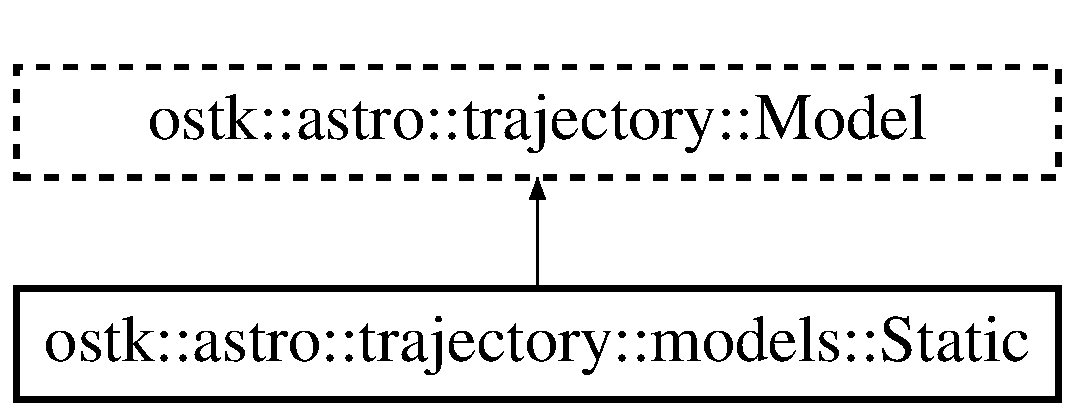
\includegraphics[height=2.000000cm]{classostk_1_1astro_1_1trajectory_1_1models_1_1_static}
\end{center}
\end{figure}
\doxysubsection*{Public Member Functions}
\begin{DoxyCompactItemize}
\item 
\mbox{\hyperlink{classostk_1_1astro_1_1trajectory_1_1models_1_1_static_a8d7240ef6b3ae12d6bdb4320b225a146}{Static}} (const Position \&a\+Position)
\item 
virtual \mbox{\hyperlink{classostk_1_1astro_1_1trajectory_1_1models_1_1_static}{Static}} $\ast$ \mbox{\hyperlink{classostk_1_1astro_1_1trajectory_1_1models_1_1_static_abe3edbc72ae2f4fbd6c2593e2aa08755}{clone}} () const override
\item 
bool \mbox{\hyperlink{classostk_1_1astro_1_1trajectory_1_1models_1_1_static_af74de1e58f8fc4373706264062a42faa}{operator==}} (const \mbox{\hyperlink{classostk_1_1astro_1_1trajectory_1_1models_1_1_static}{Static}} \&a\+Static\+Model) const
\item 
bool \mbox{\hyperlink{classostk_1_1astro_1_1trajectory_1_1models_1_1_static_af1f7415dfe8c549156734749ef4caaf4}{operator!=}} (const \mbox{\hyperlink{classostk_1_1astro_1_1trajectory_1_1models_1_1_static}{Static}} \&a\+Static\+Model) const
\item 
virtual bool \mbox{\hyperlink{classostk_1_1astro_1_1trajectory_1_1models_1_1_static_a5a80d75c9215af9b198c9f8653c5bc17}{is\+Defined}} () const override
\item 
virtual \mbox{\hyperlink{classostk_1_1astro_1_1trajectory_1_1_state}{State}} \mbox{\hyperlink{classostk_1_1astro_1_1trajectory_1_1models_1_1_static_a4297a74c953a105dc887a31227fbe1ff}{calculate\+State\+At}} (const Instant \&an\+Instant) const override
\item 
virtual void \mbox{\hyperlink{classostk_1_1astro_1_1trajectory_1_1models_1_1_static_aae663f763324f081911ea47070c9f79f}{print}} (std\+::ostream \&an\+Output\+Stream, bool display\+Decorator=true) const override
\end{DoxyCompactItemize}
\doxysubsection*{Protected Member Functions}
\begin{DoxyCompactItemize}
\item 
virtual bool \mbox{\hyperlink{classostk_1_1astro_1_1trajectory_1_1models_1_1_static_a0ef36b672baa80f522135d86f3b6bb9c}{operator==}} (const \mbox{\hyperlink{classostk_1_1astro_1_1trajectory_1_1_model}{Model}} \&a\+Model) const override
\item 
virtual bool \mbox{\hyperlink{classostk_1_1astro_1_1trajectory_1_1models_1_1_static_af85efc113db69c75c1afc7db0e81297b}{operator!=}} (const \mbox{\hyperlink{classostk_1_1astro_1_1trajectory_1_1_model}{Model}} \&a\+Model) const override
\end{DoxyCompactItemize}
\doxysubsection*{Friends}
\begin{DoxyCompactItemize}
\item 
std\+::ostream \& \mbox{\hyperlink{classostk_1_1astro_1_1trajectory_1_1models_1_1_static_a6494cb538d45101dc20cb3910455cb13}{operator$<$$<$}} (std\+::ostream \&an\+Output\+Stream, const \mbox{\hyperlink{classostk_1_1astro_1_1trajectory_1_1models_1_1_static}{Static}} \&a\+Static\+Model)
\end{DoxyCompactItemize}


\doxysubsection{Detailed Description}
\mbox{\hyperlink{classostk_1_1astro_1_1trajectory_1_1models_1_1_static}{Static}} trajectory model. 

\doxysubsection{Constructor \& Destructor Documentation}
\mbox{\Hypertarget{classostk_1_1astro_1_1trajectory_1_1models_1_1_static_a8d7240ef6b3ae12d6bdb4320b225a146}\label{classostk_1_1astro_1_1trajectory_1_1models_1_1_static_a8d7240ef6b3ae12d6bdb4320b225a146}} 
\index{ostk::astro::trajectory::models::Static@{ostk::astro::trajectory::models::Static}!Static@{Static}}
\index{Static@{Static}!ostk::astro::trajectory::models::Static@{ostk::astro::trajectory::models::Static}}
\doxysubsubsection{\texorpdfstring{Static()}{Static()}}
{\footnotesize\ttfamily ostk\+::astro\+::trajectory\+::models\+::\+Static\+::\+Static (\begin{DoxyParamCaption}\item[{const Position \&}]{a\+Position }\end{DoxyParamCaption})}



\doxysubsection{Member Function Documentation}
\mbox{\Hypertarget{classostk_1_1astro_1_1trajectory_1_1models_1_1_static_a4297a74c953a105dc887a31227fbe1ff}\label{classostk_1_1astro_1_1trajectory_1_1models_1_1_static_a4297a74c953a105dc887a31227fbe1ff}} 
\index{ostk::astro::trajectory::models::Static@{ostk::astro::trajectory::models::Static}!calculateStateAt@{calculateStateAt}}
\index{calculateStateAt@{calculateStateAt}!ostk::astro::trajectory::models::Static@{ostk::astro::trajectory::models::Static}}
\doxysubsubsection{\texorpdfstring{calculateStateAt()}{calculateStateAt()}}
{\footnotesize\ttfamily \mbox{\hyperlink{classostk_1_1astro_1_1trajectory_1_1_state}{State}} ostk\+::astro\+::trajectory\+::models\+::\+Static\+::calculate\+State\+At (\begin{DoxyParamCaption}\item[{const Instant \&}]{an\+Instant }\end{DoxyParamCaption}) const\hspace{0.3cm}{\ttfamily [override]}, {\ttfamily [virtual]}}



Implements \mbox{\hyperlink{classostk_1_1astro_1_1trajectory_1_1_model_ad25eeaded2946bf73d44161b5f4e9a0e}{ostk\+::astro\+::trajectory\+::\+Model}}.

\mbox{\Hypertarget{classostk_1_1astro_1_1trajectory_1_1models_1_1_static_abe3edbc72ae2f4fbd6c2593e2aa08755}\label{classostk_1_1astro_1_1trajectory_1_1models_1_1_static_abe3edbc72ae2f4fbd6c2593e2aa08755}} 
\index{ostk::astro::trajectory::models::Static@{ostk::astro::trajectory::models::Static}!clone@{clone}}
\index{clone@{clone}!ostk::astro::trajectory::models::Static@{ostk::astro::trajectory::models::Static}}
\doxysubsubsection{\texorpdfstring{clone()}{clone()}}
{\footnotesize\ttfamily \mbox{\hyperlink{classostk_1_1astro_1_1trajectory_1_1models_1_1_static}{Static}} $\ast$ ostk\+::astro\+::trajectory\+::models\+::\+Static\+::clone (\begin{DoxyParamCaption}{ }\end{DoxyParamCaption}) const\hspace{0.3cm}{\ttfamily [override]}, {\ttfamily [virtual]}}



Implements \mbox{\hyperlink{classostk_1_1astro_1_1trajectory_1_1_model_ad9f1467f711b07796ddc1437fb9ad9df}{ostk\+::astro\+::trajectory\+::\+Model}}.

\mbox{\Hypertarget{classostk_1_1astro_1_1trajectory_1_1models_1_1_static_a5a80d75c9215af9b198c9f8653c5bc17}\label{classostk_1_1astro_1_1trajectory_1_1models_1_1_static_a5a80d75c9215af9b198c9f8653c5bc17}} 
\index{ostk::astro::trajectory::models::Static@{ostk::astro::trajectory::models::Static}!isDefined@{isDefined}}
\index{isDefined@{isDefined}!ostk::astro::trajectory::models::Static@{ostk::astro::trajectory::models::Static}}
\doxysubsubsection{\texorpdfstring{isDefined()}{isDefined()}}
{\footnotesize\ttfamily bool ostk\+::astro\+::trajectory\+::models\+::\+Static\+::is\+Defined (\begin{DoxyParamCaption}{ }\end{DoxyParamCaption}) const\hspace{0.3cm}{\ttfamily [override]}, {\ttfamily [virtual]}}



Implements \mbox{\hyperlink{classostk_1_1astro_1_1trajectory_1_1_model_a0d5cf6f754905f06c0ec1e39618c20a1}{ostk\+::astro\+::trajectory\+::\+Model}}.

\mbox{\Hypertarget{classostk_1_1astro_1_1trajectory_1_1models_1_1_static_af85efc113db69c75c1afc7db0e81297b}\label{classostk_1_1astro_1_1trajectory_1_1models_1_1_static_af85efc113db69c75c1afc7db0e81297b}} 
\index{ostk::astro::trajectory::models::Static@{ostk::astro::trajectory::models::Static}!operator"!=@{operator"!=}}
\index{operator"!=@{operator"!=}!ostk::astro::trajectory::models::Static@{ostk::astro::trajectory::models::Static}}
\doxysubsubsection{\texorpdfstring{operator"!=()}{operator!=()}\hspace{0.1cm}{\footnotesize\ttfamily [1/2]}}
{\footnotesize\ttfamily bool ostk\+::astro\+::trajectory\+::models\+::\+Static\+::operator!= (\begin{DoxyParamCaption}\item[{const \mbox{\hyperlink{classostk_1_1astro_1_1trajectory_1_1_model}{Model}} \&}]{a\+Model }\end{DoxyParamCaption}) const\hspace{0.3cm}{\ttfamily [override]}, {\ttfamily [protected]}, {\ttfamily [virtual]}}



Implements \mbox{\hyperlink{classostk_1_1astro_1_1trajectory_1_1_model_a2dd77b9f6939d738f3a489f26c955340}{ostk\+::astro\+::trajectory\+::\+Model}}.

\mbox{\Hypertarget{classostk_1_1astro_1_1trajectory_1_1models_1_1_static_af1f7415dfe8c549156734749ef4caaf4}\label{classostk_1_1astro_1_1trajectory_1_1models_1_1_static_af1f7415dfe8c549156734749ef4caaf4}} 
\index{ostk::astro::trajectory::models::Static@{ostk::astro::trajectory::models::Static}!operator"!=@{operator"!=}}
\index{operator"!=@{operator"!=}!ostk::astro::trajectory::models::Static@{ostk::astro::trajectory::models::Static}}
\doxysubsubsection{\texorpdfstring{operator"!=()}{operator!=()}\hspace{0.1cm}{\footnotesize\ttfamily [2/2]}}
{\footnotesize\ttfamily bool ostk\+::astro\+::trajectory\+::models\+::\+Static\+::operator!= (\begin{DoxyParamCaption}\item[{const \mbox{\hyperlink{classostk_1_1astro_1_1trajectory_1_1models_1_1_static}{Static}} \&}]{a\+Static\+Model }\end{DoxyParamCaption}) const}

\mbox{\Hypertarget{classostk_1_1astro_1_1trajectory_1_1models_1_1_static_a0ef36b672baa80f522135d86f3b6bb9c}\label{classostk_1_1astro_1_1trajectory_1_1models_1_1_static_a0ef36b672baa80f522135d86f3b6bb9c}} 
\index{ostk::astro::trajectory::models::Static@{ostk::astro::trajectory::models::Static}!operator==@{operator==}}
\index{operator==@{operator==}!ostk::astro::trajectory::models::Static@{ostk::astro::trajectory::models::Static}}
\doxysubsubsection{\texorpdfstring{operator==()}{operator==()}\hspace{0.1cm}{\footnotesize\ttfamily [1/2]}}
{\footnotesize\ttfamily bool ostk\+::astro\+::trajectory\+::models\+::\+Static\+::operator== (\begin{DoxyParamCaption}\item[{const \mbox{\hyperlink{classostk_1_1astro_1_1trajectory_1_1_model}{Model}} \&}]{a\+Model }\end{DoxyParamCaption}) const\hspace{0.3cm}{\ttfamily [override]}, {\ttfamily [protected]}, {\ttfamily [virtual]}}



Implements \mbox{\hyperlink{classostk_1_1astro_1_1trajectory_1_1_model_a874f79846e845859c070ce1b9874fc9c}{ostk\+::astro\+::trajectory\+::\+Model}}.

\mbox{\Hypertarget{classostk_1_1astro_1_1trajectory_1_1models_1_1_static_af74de1e58f8fc4373706264062a42faa}\label{classostk_1_1astro_1_1trajectory_1_1models_1_1_static_af74de1e58f8fc4373706264062a42faa}} 
\index{ostk::astro::trajectory::models::Static@{ostk::astro::trajectory::models::Static}!operator==@{operator==}}
\index{operator==@{operator==}!ostk::astro::trajectory::models::Static@{ostk::astro::trajectory::models::Static}}
\doxysubsubsection{\texorpdfstring{operator==()}{operator==()}\hspace{0.1cm}{\footnotesize\ttfamily [2/2]}}
{\footnotesize\ttfamily bool ostk\+::astro\+::trajectory\+::models\+::\+Static\+::operator== (\begin{DoxyParamCaption}\item[{const \mbox{\hyperlink{classostk_1_1astro_1_1trajectory_1_1models_1_1_static}{Static}} \&}]{a\+Static\+Model }\end{DoxyParamCaption}) const}

\mbox{\Hypertarget{classostk_1_1astro_1_1trajectory_1_1models_1_1_static_aae663f763324f081911ea47070c9f79f}\label{classostk_1_1astro_1_1trajectory_1_1models_1_1_static_aae663f763324f081911ea47070c9f79f}} 
\index{ostk::astro::trajectory::models::Static@{ostk::astro::trajectory::models::Static}!print@{print}}
\index{print@{print}!ostk::astro::trajectory::models::Static@{ostk::astro::trajectory::models::Static}}
\doxysubsubsection{\texorpdfstring{print()}{print()}}
{\footnotesize\ttfamily void ostk\+::astro\+::trajectory\+::models\+::\+Static\+::print (\begin{DoxyParamCaption}\item[{std\+::ostream \&}]{an\+Output\+Stream,  }\item[{bool}]{display\+Decorator = {\ttfamily true} }\end{DoxyParamCaption}) const\hspace{0.3cm}{\ttfamily [override]}, {\ttfamily [virtual]}}



Implements \mbox{\hyperlink{classostk_1_1astro_1_1trajectory_1_1_model_a4b2098483430a820481ed50b81656e31}{ostk\+::astro\+::trajectory\+::\+Model}}.



\doxysubsection{Friends And Related Function Documentation}
\mbox{\Hypertarget{classostk_1_1astro_1_1trajectory_1_1models_1_1_static_a6494cb538d45101dc20cb3910455cb13}\label{classostk_1_1astro_1_1trajectory_1_1models_1_1_static_a6494cb538d45101dc20cb3910455cb13}} 
\index{ostk::astro::trajectory::models::Static@{ostk::astro::trajectory::models::Static}!operator$<$$<$@{operator$<$$<$}}
\index{operator$<$$<$@{operator$<$$<$}!ostk::astro::trajectory::models::Static@{ostk::astro::trajectory::models::Static}}
\doxysubsubsection{\texorpdfstring{operator$<$$<$}{operator<<}}
{\footnotesize\ttfamily std\+::ostream\& operator$<$$<$ (\begin{DoxyParamCaption}\item[{std\+::ostream \&}]{an\+Output\+Stream,  }\item[{const \mbox{\hyperlink{classostk_1_1astro_1_1trajectory_1_1models_1_1_static}{Static}} \&}]{a\+Static\+Model }\end{DoxyParamCaption})\hspace{0.3cm}{\ttfamily [friend]}}



The documentation for this class was generated from the following files\+:\begin{DoxyCompactItemize}
\item 
include/\+Open\+Space\+Toolkit/\+Astrodynamics/\+Trajectory/\+Models/\mbox{\hyperlink{_static_8hpp}{Static.\+hpp}}\item 
src/\+Open\+Space\+Toolkit/\+Astrodynamics/\+Trajectory/\+Models/\mbox{\hyperlink{_static_8cpp}{Static.\+cpp}}\end{DoxyCompactItemize}

\hypertarget{classostk_1_1astro_1_1flight_1_1_system}{}\doxysection{ostk\+::astro\+::flight\+::System Class Reference}
\label{classostk_1_1astro_1_1flight_1_1_system}\index{ostk::astro::flight::System@{ostk::astro::flight::System}}


Defines the generic physical system that has a mass and a certain geometry that can be composed of multiple subgeometries.  




{\ttfamily \#include $<$System.\+hpp$>$}

Inheritance diagram for ostk\+::astro\+::flight\+::System\+:\begin{figure}[H]
\begin{center}
\leavevmode
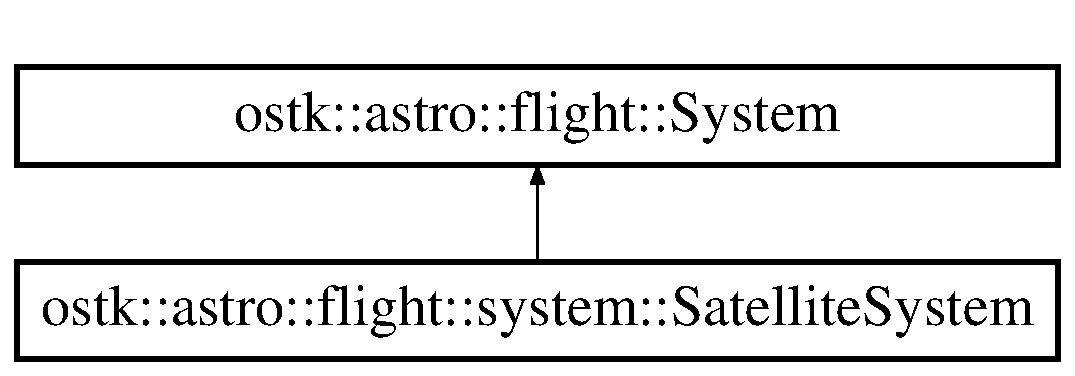
\includegraphics[height=2.000000cm]{classostk_1_1astro_1_1flight_1_1_system}
\end{center}
\end{figure}
\doxysubsection*{Public Member Functions}
\begin{DoxyCompactItemize}
\item 
\mbox{\hyperlink{classostk_1_1astro_1_1flight_1_1_system_afac17c0d5e2b1fb9416babf240a1aa65}{System}} (const Mass \&a\+Mass, const Composite \&a\+Geometry)
\begin{DoxyCompactList}\small\item\em Constructor. \end{DoxyCompactList}\item 
virtual \mbox{\hyperlink{classostk_1_1astro_1_1flight_1_1_system_a465eb91f18cbc10466b30694daab39fd}{$\sim$\+System}} ()
\begin{DoxyCompactList}\small\item\em Destructor. \end{DoxyCompactList}\item 
\mbox{\hyperlink{classostk_1_1astro_1_1flight_1_1_system}{System}} $\ast$ \mbox{\hyperlink{classostk_1_1astro_1_1flight_1_1_system_ade321754db6db7f635def34cb137d9c4}{clone}} () const
\begin{DoxyCompactList}\small\item\em Clone system. \end{DoxyCompactList}\item 
bool \mbox{\hyperlink{classostk_1_1astro_1_1flight_1_1_system_a8d8602da9451044f9810eaf22076b852}{operator==}} (const \mbox{\hyperlink{classostk_1_1astro_1_1flight_1_1_system}{System}} \&a\+System) const
\begin{DoxyCompactList}\small\item\em Equal to operator. \end{DoxyCompactList}\item 
bool \mbox{\hyperlink{classostk_1_1astro_1_1flight_1_1_system_a5426b85c139cf30be998e0a983fe5978}{operator!=}} (const \mbox{\hyperlink{classostk_1_1astro_1_1flight_1_1_system}{System}} \&a\+System) const
\begin{DoxyCompactList}\small\item\em Not equal to operator. \end{DoxyCompactList}\item 
virtual bool \mbox{\hyperlink{classostk_1_1astro_1_1flight_1_1_system_a45d6ad6bca50c0d9cb9b50135ed2efa3}{is\+Defined}} () const
\begin{DoxyCompactList}\small\item\em Check if system is defined. \end{DoxyCompactList}\item 
virtual void \mbox{\hyperlink{classostk_1_1astro_1_1flight_1_1_system_a24d1aacf9355f5ee56fa56eeabe231ab}{print}} (std\+::ostream \&an\+Output\+Stream, bool display\+Decorator=true) const
\begin{DoxyCompactList}\small\item\em Print system. \end{DoxyCompactList}\item 
Mass \mbox{\hyperlink{classostk_1_1astro_1_1flight_1_1_system_a5c83b22d462c5d4b3f9766430c17d646}{get\+Mass}} () const
\begin{DoxyCompactList}\small\item\em Get system\textquotesingle{}s mass. \end{DoxyCompactList}\item 
Composite \mbox{\hyperlink{classostk_1_1astro_1_1flight_1_1_system_ac50685f33e3442384ed41b3b8c2d6549}{get\+Geometry}} () const
\begin{DoxyCompactList}\small\item\em Get system\textquotesingle{}s geometry. \end{DoxyCompactList}\end{DoxyCompactItemize}
\doxysubsection*{Static Public Member Functions}
\begin{DoxyCompactItemize}
\item 
static \mbox{\hyperlink{classostk_1_1astro_1_1flight_1_1_system}{System}} \mbox{\hyperlink{classostk_1_1astro_1_1flight_1_1_system_abb1e68e42b4791d7268e18608c8909af}{Undefined}} ()
\end{DoxyCompactItemize}
\doxysubsection*{Friends}
\begin{DoxyCompactItemize}
\item 
std\+::ostream \& \mbox{\hyperlink{classostk_1_1astro_1_1flight_1_1_system_aaf88422b640217e9e1c2c354a7e05634}{operator$<$$<$}} (std\+::ostream \&an\+Output\+Stream, const \mbox{\hyperlink{classostk_1_1astro_1_1flight_1_1_system}{System}} \&a\+System)
\begin{DoxyCompactList}\small\item\em Output stream operator. \end{DoxyCompactList}\end{DoxyCompactItemize}


\doxysubsection{Detailed Description}
Defines the generic physical system that has a mass and a certain geometry that can be composed of multiple subgeometries. 

\doxysubsection{Constructor \& Destructor Documentation}
\mbox{\Hypertarget{classostk_1_1astro_1_1flight_1_1_system_afac17c0d5e2b1fb9416babf240a1aa65}\label{classostk_1_1astro_1_1flight_1_1_system_afac17c0d5e2b1fb9416babf240a1aa65}} 
\index{ostk::astro::flight::System@{ostk::astro::flight::System}!System@{System}}
\index{System@{System}!ostk::astro::flight::System@{ostk::astro::flight::System}}
\doxysubsubsection{\texorpdfstring{System()}{System()}}
{\footnotesize\ttfamily ostk\+::astro\+::flight\+::\+System\+::\+System (\begin{DoxyParamCaption}\item[{const Mass \&}]{a\+Mass,  }\item[{const Composite \&}]{a\+Geometry }\end{DoxyParamCaption})}



Constructor. 


\begin{DoxyCode}{0}
\DoxyCodeLine{Mass mass = \{ ... \} ;}
\DoxyCodeLine{Composite composite ( ... ) ;}
\DoxyCodeLine{\mbox{\hyperlink{classostk_1_1astro_1_1flight_1_1_system_afac17c0d5e2b1fb9416babf240a1aa65}{System}} system = \{ mass, composite \} ;}
\end{DoxyCode}



\begin{DoxyParams}{Parameters}
{\em a\+Mass} & A mass \\
\hline
{\em a\+Geometry} & A geometry \\
\hline
\end{DoxyParams}
\mbox{\Hypertarget{classostk_1_1astro_1_1flight_1_1_system_a465eb91f18cbc10466b30694daab39fd}\label{classostk_1_1astro_1_1flight_1_1_system_a465eb91f18cbc10466b30694daab39fd}} 
\index{ostk::astro::flight::System@{ostk::astro::flight::System}!````~System@{$\sim$System}}
\index{````~System@{$\sim$System}!ostk::astro::flight::System@{ostk::astro::flight::System}}
\doxysubsubsection{\texorpdfstring{$\sim$System()}{~System()}}
{\footnotesize\ttfamily ostk\+::astro\+::flight\+::\+System\+::$\sim$\+System (\begin{DoxyParamCaption}{ }\end{DoxyParamCaption})\hspace{0.3cm}{\ttfamily [virtual]}}



Destructor. 



\doxysubsection{Member Function Documentation}
\mbox{\Hypertarget{classostk_1_1astro_1_1flight_1_1_system_ade321754db6db7f635def34cb137d9c4}\label{classostk_1_1astro_1_1flight_1_1_system_ade321754db6db7f635def34cb137d9c4}} 
\index{ostk::astro::flight::System@{ostk::astro::flight::System}!clone@{clone}}
\index{clone@{clone}!ostk::astro::flight::System@{ostk::astro::flight::System}}
\doxysubsubsection{\texorpdfstring{clone()}{clone()}}
{\footnotesize\ttfamily \mbox{\hyperlink{classostk_1_1astro_1_1flight_1_1_system}{System}} $\ast$ ostk\+::astro\+::flight\+::\+System\+::clone (\begin{DoxyParamCaption}{ }\end{DoxyParamCaption}) const}



Clone system. 

\begin{DoxyReturn}{Returns}
Pointer to cloned system 
\end{DoxyReturn}
\mbox{\Hypertarget{classostk_1_1astro_1_1flight_1_1_system_ac50685f33e3442384ed41b3b8c2d6549}\label{classostk_1_1astro_1_1flight_1_1_system_ac50685f33e3442384ed41b3b8c2d6549}} 
\index{ostk::astro::flight::System@{ostk::astro::flight::System}!getGeometry@{getGeometry}}
\index{getGeometry@{getGeometry}!ostk::astro::flight::System@{ostk::astro::flight::System}}
\doxysubsubsection{\texorpdfstring{getGeometry()}{getGeometry()}}
{\footnotesize\ttfamily Composite ostk\+::astro\+::flight\+::\+System\+::get\+Geometry (\begin{DoxyParamCaption}{ }\end{DoxyParamCaption}) const}



Get system\textquotesingle{}s geometry. 


\begin{DoxyCode}{0}
\DoxyCodeLine{Mass mass = system.getGeometry() ;}
\end{DoxyCode}


\begin{DoxyReturn}{Returns}
Composite 
\end{DoxyReturn}
\mbox{\Hypertarget{classostk_1_1astro_1_1flight_1_1_system_a5c83b22d462c5d4b3f9766430c17d646}\label{classostk_1_1astro_1_1flight_1_1_system_a5c83b22d462c5d4b3f9766430c17d646}} 
\index{ostk::astro::flight::System@{ostk::astro::flight::System}!getMass@{getMass}}
\index{getMass@{getMass}!ostk::astro::flight::System@{ostk::astro::flight::System}}
\doxysubsubsection{\texorpdfstring{getMass()}{getMass()}}
{\footnotesize\ttfamily Mass ostk\+::astro\+::flight\+::\+System\+::get\+Mass (\begin{DoxyParamCaption}{ }\end{DoxyParamCaption}) const}



Get system\textquotesingle{}s mass. 


\begin{DoxyCode}{0}
\DoxyCodeLine{Mass mass = system.getMass() ;}
\end{DoxyCode}


\begin{DoxyReturn}{Returns}
Mass 
\end{DoxyReturn}
\mbox{\Hypertarget{classostk_1_1astro_1_1flight_1_1_system_a45d6ad6bca50c0d9cb9b50135ed2efa3}\label{classostk_1_1astro_1_1flight_1_1_system_a45d6ad6bca50c0d9cb9b50135ed2efa3}} 
\index{ostk::astro::flight::System@{ostk::astro::flight::System}!isDefined@{isDefined}}
\index{isDefined@{isDefined}!ostk::astro::flight::System@{ostk::astro::flight::System}}
\doxysubsubsection{\texorpdfstring{isDefined()}{isDefined()}}
{\footnotesize\ttfamily bool ostk\+::astro\+::flight\+::\+System\+::is\+Defined (\begin{DoxyParamCaption}{ }\end{DoxyParamCaption}) const\hspace{0.3cm}{\ttfamily [virtual]}}



Check if system is defined. 

\begin{DoxyReturn}{Returns}
True if system is defined 
\end{DoxyReturn}


Reimplemented in \mbox{\hyperlink{classostk_1_1astro_1_1flight_1_1system_1_1_satellite_system_a6d10fc37776cc87a74fe8b7e2ccb9843}{ostk\+::astro\+::flight\+::system\+::\+Satellite\+System}}.

\mbox{\Hypertarget{classostk_1_1astro_1_1flight_1_1_system_a5426b85c139cf30be998e0a983fe5978}\label{classostk_1_1astro_1_1flight_1_1_system_a5426b85c139cf30be998e0a983fe5978}} 
\index{ostk::astro::flight::System@{ostk::astro::flight::System}!operator"!=@{operator"!=}}
\index{operator"!=@{operator"!=}!ostk::astro::flight::System@{ostk::astro::flight::System}}
\doxysubsubsection{\texorpdfstring{operator"!=()}{operator!=()}}
{\footnotesize\ttfamily bool ostk\+::astro\+::flight\+::\+System\+::operator!= (\begin{DoxyParamCaption}\item[{const \mbox{\hyperlink{classostk_1_1astro_1_1flight_1_1_system}{System}} \&}]{a\+System }\end{DoxyParamCaption}) const}



Not equal to operator. 


\begin{DoxyParams}{Parameters}
{\em a\+System} & A system \\
\hline
\end{DoxyParams}
\begin{DoxyReturn}{Returns}
True if systems are not equal 
\end{DoxyReturn}
\mbox{\Hypertarget{classostk_1_1astro_1_1flight_1_1_system_a8d8602da9451044f9810eaf22076b852}\label{classostk_1_1astro_1_1flight_1_1_system_a8d8602da9451044f9810eaf22076b852}} 
\index{ostk::astro::flight::System@{ostk::astro::flight::System}!operator==@{operator==}}
\index{operator==@{operator==}!ostk::astro::flight::System@{ostk::astro::flight::System}}
\doxysubsubsection{\texorpdfstring{operator==()}{operator==()}}
{\footnotesize\ttfamily bool ostk\+::astro\+::flight\+::\+System\+::operator== (\begin{DoxyParamCaption}\item[{const \mbox{\hyperlink{classostk_1_1astro_1_1flight_1_1_system}{System}} \&}]{a\+System }\end{DoxyParamCaption}) const}



Equal to operator. 


\begin{DoxyParams}{Parameters}
{\em a\+System} & A system \\
\hline
\end{DoxyParams}
\begin{DoxyReturn}{Returns}
True if systems are equal 
\end{DoxyReturn}
\mbox{\Hypertarget{classostk_1_1astro_1_1flight_1_1_system_a24d1aacf9355f5ee56fa56eeabe231ab}\label{classostk_1_1astro_1_1flight_1_1_system_a24d1aacf9355f5ee56fa56eeabe231ab}} 
\index{ostk::astro::flight::System@{ostk::astro::flight::System}!print@{print}}
\index{print@{print}!ostk::astro::flight::System@{ostk::astro::flight::System}}
\doxysubsubsection{\texorpdfstring{print()}{print()}}
{\footnotesize\ttfamily void ostk\+::astro\+::flight\+::\+System\+::print (\begin{DoxyParamCaption}\item[{std\+::ostream \&}]{an\+Output\+Stream,  }\item[{bool}]{display\+Decorator = {\ttfamily true} }\end{DoxyParamCaption}) const\hspace{0.3cm}{\ttfamily [virtual]}}



Print system. 


\begin{DoxyParams}{Parameters}
{\em an\+Output\+Stream} & An output stream \\
\hline
{\em (optional)} & display\+Decorators If true, display decorators \\
\hline
\end{DoxyParams}


Reimplemented in \mbox{\hyperlink{classostk_1_1astro_1_1flight_1_1system_1_1_satellite_system_a0d4ca06c426773f667018581945dbf57}{ostk\+::astro\+::flight\+::system\+::\+Satellite\+System}}.

\mbox{\Hypertarget{classostk_1_1astro_1_1flight_1_1_system_abb1e68e42b4791d7268e18608c8909af}\label{classostk_1_1astro_1_1flight_1_1_system_abb1e68e42b4791d7268e18608c8909af}} 
\index{ostk::astro::flight::System@{ostk::astro::flight::System}!Undefined@{Undefined}}
\index{Undefined@{Undefined}!ostk::astro::flight::System@{ostk::astro::flight::System}}
\doxysubsubsection{\texorpdfstring{Undefined()}{Undefined()}}
{\footnotesize\ttfamily \mbox{\hyperlink{classostk_1_1astro_1_1flight_1_1_system}{System}} ostk\+::astro\+::flight\+::\+System\+::\+Undefined (\begin{DoxyParamCaption}{ }\end{DoxyParamCaption})\hspace{0.3cm}{\ttfamily [static]}}



\doxysubsection{Friends And Related Function Documentation}
\mbox{\Hypertarget{classostk_1_1astro_1_1flight_1_1_system_aaf88422b640217e9e1c2c354a7e05634}\label{classostk_1_1astro_1_1flight_1_1_system_aaf88422b640217e9e1c2c354a7e05634}} 
\index{ostk::astro::flight::System@{ostk::astro::flight::System}!operator$<$$<$@{operator$<$$<$}}
\index{operator$<$$<$@{operator$<$$<$}!ostk::astro::flight::System@{ostk::astro::flight::System}}
\doxysubsubsection{\texorpdfstring{operator$<$$<$}{operator<<}}
{\footnotesize\ttfamily std\+::ostream\& operator$<$$<$ (\begin{DoxyParamCaption}\item[{std\+::ostream \&}]{an\+Output\+Stream,  }\item[{const \mbox{\hyperlink{classostk_1_1astro_1_1flight_1_1_system}{System}} \&}]{a\+System }\end{DoxyParamCaption})\hspace{0.3cm}{\ttfamily [friend]}}



Output stream operator. 


\begin{DoxyParams}{Parameters}
{\em an\+Output\+Stream} & An output stream \\
\hline
{\em a\+System} & A system \\
\hline
\end{DoxyParams}
\begin{DoxyReturn}{Returns}
A reference to output stream 
\end{DoxyReturn}


The documentation for this class was generated from the following files\+:\begin{DoxyCompactItemize}
\item 
include/\+Open\+Space\+Toolkit/\+Astrodynamics/\+Flight/\mbox{\hyperlink{_system_8hpp}{System.\+hpp}}\item 
src/\+Open\+Space\+Toolkit/\+Astrodynamics/\+Flight/\mbox{\hyperlink{_system_8cpp}{System.\+cpp}}\end{DoxyCompactItemize}

\hypertarget{classostk_1_1astro_1_1flight_1_1profile_1_1models_1_1_tabulated}{}\doxysection{ostk\+::astro\+::flight\+::profile\+::models\+::Tabulated Class Reference}
\label{classostk_1_1astro_1_1flight_1_1profile_1_1models_1_1_tabulated}\index{ostk::astro::flight::profile::models::Tabulated@{ostk::astro::flight::profile::models::Tabulated}}


\mbox{\hyperlink{classostk_1_1astro_1_1flight_1_1profile_1_1models_1_1_tabulated}{Tabulated}} profile model.  




{\ttfamily \#include $<$Tabulated.\+hpp$>$}

Inheritance diagram for ostk\+::astro\+::flight\+::profile\+::models\+::Tabulated\+:\begin{figure}[H]
\begin{center}
\leavevmode
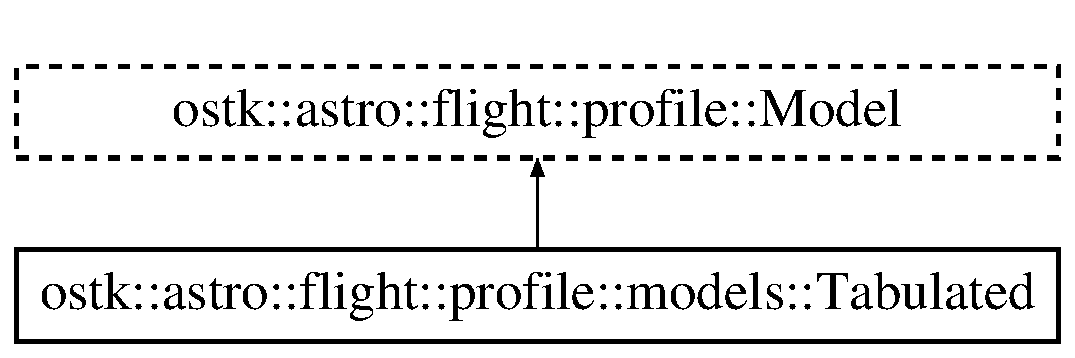
\includegraphics[height=2.000000cm]{classostk_1_1astro_1_1flight_1_1profile_1_1models_1_1_tabulated}
\end{center}
\end{figure}
\doxysubsection*{Public Member Functions}
\begin{DoxyCompactItemize}
\item 
\mbox{\hyperlink{classostk_1_1astro_1_1flight_1_1profile_1_1models_1_1_tabulated_a68153fb9d50b8ed216c5635304a2f433}{Tabulated}} (const Array$<$ \mbox{\hyperlink{classostk_1_1astro_1_1flight_1_1profile_1_1_state}{State}} $>$ \&a\+State\+Array)
\item 
virtual \mbox{\hyperlink{classostk_1_1astro_1_1flight_1_1profile_1_1models_1_1_tabulated}{Tabulated}} $\ast$ \mbox{\hyperlink{classostk_1_1astro_1_1flight_1_1profile_1_1models_1_1_tabulated_a1c9f4f5711ac2ae0cc545d89b0ee4d53}{clone}} () const override
\item 
bool \mbox{\hyperlink{classostk_1_1astro_1_1flight_1_1profile_1_1models_1_1_tabulated_a45e872950f1a20fad948295fb6b9ac7f}{operator==}} (const \mbox{\hyperlink{classostk_1_1astro_1_1flight_1_1profile_1_1models_1_1_tabulated}{Tabulated}} \&a\+Tabulated\+Model) const
\item 
virtual bool \mbox{\hyperlink{classostk_1_1astro_1_1flight_1_1profile_1_1models_1_1_tabulated_ad830d557475ca2ba83d43659e348b1d6}{is\+Defined}} () const override
\item 
Interval \mbox{\hyperlink{classostk_1_1astro_1_1flight_1_1profile_1_1models_1_1_tabulated_abf25afb50a324162903488374c4df078}{get\+Interval}} () const
\item 
virtual \mbox{\hyperlink{classostk_1_1astro_1_1flight_1_1profile_1_1_state}{State}} \mbox{\hyperlink{classostk_1_1astro_1_1flight_1_1profile_1_1models_1_1_tabulated_af27ea0e7006d0de18e897a9a5c7a0fb2}{calculate\+State\+At}} (const Instant \&an\+Instant) const override
\item 
virtual Axes \mbox{\hyperlink{classostk_1_1astro_1_1flight_1_1profile_1_1models_1_1_tabulated_ac85970f439c8db0684c9349601c226d2}{get\+Axes\+At}} (const Instant \&an\+Instant) const override
\item 
virtual Shared$<$ const Frame $>$ \mbox{\hyperlink{classostk_1_1astro_1_1flight_1_1profile_1_1models_1_1_tabulated_a1be1d71748e4e0b59bd3dd2334b759fe}{get\+Body\+Frame}} (const String \&a\+Frame\+Name) const override
\item 
virtual void \mbox{\hyperlink{classostk_1_1astro_1_1flight_1_1profile_1_1models_1_1_tabulated_a0e3d34c39a644279a9b958c3fd9bf730}{print}} (std\+::ostream \&an\+Output\+Stream, bool display\+Decorator=true) const override
\end{DoxyCompactItemize}
\doxysubsection*{Static Public Member Functions}
\begin{DoxyCompactItemize}
\item 
static \mbox{\hyperlink{classostk_1_1astro_1_1flight_1_1profile_1_1models_1_1_tabulated}{Tabulated}} \mbox{\hyperlink{classostk_1_1astro_1_1flight_1_1profile_1_1models_1_1_tabulated_a23496ff93340b9a483b5154027824b42}{Load}} (const File \&a\+File)
\end{DoxyCompactItemize}
\doxysubsection*{Protected Member Functions}
\begin{DoxyCompactItemize}
\item 
virtual bool \mbox{\hyperlink{classostk_1_1astro_1_1flight_1_1profile_1_1models_1_1_tabulated_a5fd04ff2470cfe517bcb94e70fdb80fd}{operator==}} (const \mbox{\hyperlink{classostk_1_1astro_1_1flight_1_1profile_1_1_model}{Model}} \&a\+Model) const override
\item 
virtual bool \mbox{\hyperlink{classostk_1_1astro_1_1flight_1_1profile_1_1models_1_1_tabulated_a7d1f3f2024628e03eee408eaa1cd1a9b}{operator!=}} (const \mbox{\hyperlink{classostk_1_1astro_1_1flight_1_1profile_1_1_model}{Model}} \&a\+Model) const override
\end{DoxyCompactItemize}
\doxysubsection*{Friends}
\begin{DoxyCompactItemize}
\item 
std\+::ostream \& \mbox{\hyperlink{classostk_1_1astro_1_1flight_1_1profile_1_1models_1_1_tabulated_af2b779226be02822defbe40cf6d3c4b8}{operator$<$$<$}} (std\+::ostream \&an\+Output\+Stream, const \mbox{\hyperlink{classostk_1_1astro_1_1flight_1_1profile_1_1models_1_1_tabulated}{Tabulated}} \&a\+Tabulated\+Model)
\end{DoxyCompactItemize}


\doxysubsection{Detailed Description}
\mbox{\hyperlink{classostk_1_1astro_1_1flight_1_1profile_1_1models_1_1_tabulated}{Tabulated}} profile model. 

\doxysubsection{Constructor \& Destructor Documentation}
\mbox{\Hypertarget{classostk_1_1astro_1_1flight_1_1profile_1_1models_1_1_tabulated_a68153fb9d50b8ed216c5635304a2f433}\label{classostk_1_1astro_1_1flight_1_1profile_1_1models_1_1_tabulated_a68153fb9d50b8ed216c5635304a2f433}} 
\index{ostk::astro::flight::profile::models::Tabulated@{ostk::astro::flight::profile::models::Tabulated}!Tabulated@{Tabulated}}
\index{Tabulated@{Tabulated}!ostk::astro::flight::profile::models::Tabulated@{ostk::astro::flight::profile::models::Tabulated}}
\doxysubsubsection{\texorpdfstring{Tabulated()}{Tabulated()}}
{\footnotesize\ttfamily ostk\+::astro\+::flight\+::profile\+::models\+::\+Tabulated\+::\+Tabulated (\begin{DoxyParamCaption}\item[{const Array$<$ \mbox{\hyperlink{classostk_1_1astro_1_1flight_1_1profile_1_1_state}{State}} $>$ \&}]{a\+State\+Array }\end{DoxyParamCaption})}



\doxysubsection{Member Function Documentation}
\mbox{\Hypertarget{classostk_1_1astro_1_1flight_1_1profile_1_1models_1_1_tabulated_af27ea0e7006d0de18e897a9a5c7a0fb2}\label{classostk_1_1astro_1_1flight_1_1profile_1_1models_1_1_tabulated_af27ea0e7006d0de18e897a9a5c7a0fb2}} 
\index{ostk::astro::flight::profile::models::Tabulated@{ostk::astro::flight::profile::models::Tabulated}!calculateStateAt@{calculateStateAt}}
\index{calculateStateAt@{calculateStateAt}!ostk::astro::flight::profile::models::Tabulated@{ostk::astro::flight::profile::models::Tabulated}}
\doxysubsubsection{\texorpdfstring{calculateStateAt()}{calculateStateAt()}}
{\footnotesize\ttfamily \mbox{\hyperlink{classostk_1_1astro_1_1flight_1_1profile_1_1_state}{State}} ostk\+::astro\+::flight\+::profile\+::models\+::\+Tabulated\+::calculate\+State\+At (\begin{DoxyParamCaption}\item[{const Instant \&}]{an\+Instant }\end{DoxyParamCaption}) const\hspace{0.3cm}{\ttfamily [override]}, {\ttfamily [virtual]}}



Implements \mbox{\hyperlink{classostk_1_1astro_1_1flight_1_1profile_1_1_model_a1b205fa29b50fcfc06c99234a8579eb8}{ostk\+::astro\+::flight\+::profile\+::\+Model}}.

\mbox{\Hypertarget{classostk_1_1astro_1_1flight_1_1profile_1_1models_1_1_tabulated_a1c9f4f5711ac2ae0cc545d89b0ee4d53}\label{classostk_1_1astro_1_1flight_1_1profile_1_1models_1_1_tabulated_a1c9f4f5711ac2ae0cc545d89b0ee4d53}} 
\index{ostk::astro::flight::profile::models::Tabulated@{ostk::astro::flight::profile::models::Tabulated}!clone@{clone}}
\index{clone@{clone}!ostk::astro::flight::profile::models::Tabulated@{ostk::astro::flight::profile::models::Tabulated}}
\doxysubsubsection{\texorpdfstring{clone()}{clone()}}
{\footnotesize\ttfamily \mbox{\hyperlink{classostk_1_1astro_1_1flight_1_1profile_1_1models_1_1_tabulated}{Tabulated}} $\ast$ ostk\+::astro\+::flight\+::profile\+::models\+::\+Tabulated\+::clone (\begin{DoxyParamCaption}{ }\end{DoxyParamCaption}) const\hspace{0.3cm}{\ttfamily [override]}, {\ttfamily [virtual]}}



Implements \mbox{\hyperlink{classostk_1_1astro_1_1flight_1_1profile_1_1_model_aabf68c114849fa16a570b694579da40f}{ostk\+::astro\+::flight\+::profile\+::\+Model}}.

\mbox{\Hypertarget{classostk_1_1astro_1_1flight_1_1profile_1_1models_1_1_tabulated_ac85970f439c8db0684c9349601c226d2}\label{classostk_1_1astro_1_1flight_1_1profile_1_1models_1_1_tabulated_ac85970f439c8db0684c9349601c226d2}} 
\index{ostk::astro::flight::profile::models::Tabulated@{ostk::astro::flight::profile::models::Tabulated}!getAxesAt@{getAxesAt}}
\index{getAxesAt@{getAxesAt}!ostk::astro::flight::profile::models::Tabulated@{ostk::astro::flight::profile::models::Tabulated}}
\doxysubsubsection{\texorpdfstring{getAxesAt()}{getAxesAt()}}
{\footnotesize\ttfamily Axes ostk\+::astro\+::flight\+::profile\+::models\+::\+Tabulated\+::get\+Axes\+At (\begin{DoxyParamCaption}\item[{const Instant \&}]{an\+Instant }\end{DoxyParamCaption}) const\hspace{0.3cm}{\ttfamily [override]}, {\ttfamily [virtual]}}



Implements \mbox{\hyperlink{classostk_1_1astro_1_1flight_1_1profile_1_1_model_ab18bd79e421c36df4ab716649ce549cd}{ostk\+::astro\+::flight\+::profile\+::\+Model}}.

\mbox{\Hypertarget{classostk_1_1astro_1_1flight_1_1profile_1_1models_1_1_tabulated_a1be1d71748e4e0b59bd3dd2334b759fe}\label{classostk_1_1astro_1_1flight_1_1profile_1_1models_1_1_tabulated_a1be1d71748e4e0b59bd3dd2334b759fe}} 
\index{ostk::astro::flight::profile::models::Tabulated@{ostk::astro::flight::profile::models::Tabulated}!getBodyFrame@{getBodyFrame}}
\index{getBodyFrame@{getBodyFrame}!ostk::astro::flight::profile::models::Tabulated@{ostk::astro::flight::profile::models::Tabulated}}
\doxysubsubsection{\texorpdfstring{getBodyFrame()}{getBodyFrame()}}
{\footnotesize\ttfamily Shared$<$ const Frame $>$ ostk\+::astro\+::flight\+::profile\+::models\+::\+Tabulated\+::get\+Body\+Frame (\begin{DoxyParamCaption}\item[{const String \&}]{a\+Frame\+Name }\end{DoxyParamCaption}) const\hspace{0.3cm}{\ttfamily [override]}, {\ttfamily [virtual]}}



Implements \mbox{\hyperlink{classostk_1_1astro_1_1flight_1_1profile_1_1_model_a04ded49c09d9a44820251c48f47d0ffa}{ostk\+::astro\+::flight\+::profile\+::\+Model}}.

\mbox{\Hypertarget{classostk_1_1astro_1_1flight_1_1profile_1_1models_1_1_tabulated_abf25afb50a324162903488374c4df078}\label{classostk_1_1astro_1_1flight_1_1profile_1_1models_1_1_tabulated_abf25afb50a324162903488374c4df078}} 
\index{ostk::astro::flight::profile::models::Tabulated@{ostk::astro::flight::profile::models::Tabulated}!getInterval@{getInterval}}
\index{getInterval@{getInterval}!ostk::astro::flight::profile::models::Tabulated@{ostk::astro::flight::profile::models::Tabulated}}
\doxysubsubsection{\texorpdfstring{getInterval()}{getInterval()}}
{\footnotesize\ttfamily Interval ostk\+::astro\+::flight\+::profile\+::models\+::\+Tabulated\+::get\+Interval (\begin{DoxyParamCaption}{ }\end{DoxyParamCaption}) const}

\mbox{\Hypertarget{classostk_1_1astro_1_1flight_1_1profile_1_1models_1_1_tabulated_ad830d557475ca2ba83d43659e348b1d6}\label{classostk_1_1astro_1_1flight_1_1profile_1_1models_1_1_tabulated_ad830d557475ca2ba83d43659e348b1d6}} 
\index{ostk::astro::flight::profile::models::Tabulated@{ostk::astro::flight::profile::models::Tabulated}!isDefined@{isDefined}}
\index{isDefined@{isDefined}!ostk::astro::flight::profile::models::Tabulated@{ostk::astro::flight::profile::models::Tabulated}}
\doxysubsubsection{\texorpdfstring{isDefined()}{isDefined()}}
{\footnotesize\ttfamily bool ostk\+::astro\+::flight\+::profile\+::models\+::\+Tabulated\+::is\+Defined (\begin{DoxyParamCaption}{ }\end{DoxyParamCaption}) const\hspace{0.3cm}{\ttfamily [override]}, {\ttfamily [virtual]}}



Implements \mbox{\hyperlink{classostk_1_1astro_1_1flight_1_1profile_1_1_model_a0af64ad25ed8d8b2510a70bfe5bcb971}{ostk\+::astro\+::flight\+::profile\+::\+Model}}.

\mbox{\Hypertarget{classostk_1_1astro_1_1flight_1_1profile_1_1models_1_1_tabulated_a23496ff93340b9a483b5154027824b42}\label{classostk_1_1astro_1_1flight_1_1profile_1_1models_1_1_tabulated_a23496ff93340b9a483b5154027824b42}} 
\index{ostk::astro::flight::profile::models::Tabulated@{ostk::astro::flight::profile::models::Tabulated}!Load@{Load}}
\index{Load@{Load}!ostk::astro::flight::profile::models::Tabulated@{ostk::astro::flight::profile::models::Tabulated}}
\doxysubsubsection{\texorpdfstring{Load()}{Load()}}
{\footnotesize\ttfamily static \mbox{\hyperlink{classostk_1_1astro_1_1flight_1_1profile_1_1models_1_1_tabulated}{Tabulated}} ostk\+::astro\+::flight\+::profile\+::models\+::\+Tabulated\+::\+Load (\begin{DoxyParamCaption}\item[{const File \&}]{a\+File }\end{DoxyParamCaption})\hspace{0.3cm}{\ttfamily [static]}}

\mbox{\Hypertarget{classostk_1_1astro_1_1flight_1_1profile_1_1models_1_1_tabulated_a7d1f3f2024628e03eee408eaa1cd1a9b}\label{classostk_1_1astro_1_1flight_1_1profile_1_1models_1_1_tabulated_a7d1f3f2024628e03eee408eaa1cd1a9b}} 
\index{ostk::astro::flight::profile::models::Tabulated@{ostk::astro::flight::profile::models::Tabulated}!operator"!=@{operator"!=}}
\index{operator"!=@{operator"!=}!ostk::astro::flight::profile::models::Tabulated@{ostk::astro::flight::profile::models::Tabulated}}
\doxysubsubsection{\texorpdfstring{operator"!=()}{operator!=()}}
{\footnotesize\ttfamily bool ostk\+::astro\+::flight\+::profile\+::models\+::\+Tabulated\+::operator!= (\begin{DoxyParamCaption}\item[{const \mbox{\hyperlink{classostk_1_1astro_1_1flight_1_1profile_1_1_model}{Model}} \&}]{a\+Model }\end{DoxyParamCaption}) const\hspace{0.3cm}{\ttfamily [override]}, {\ttfamily [protected]}, {\ttfamily [virtual]}}



Reimplemented from \mbox{\hyperlink{classostk_1_1astro_1_1flight_1_1profile_1_1_model_a66eab26e18de60c179529ba5924b168f}{ostk\+::astro\+::flight\+::profile\+::\+Model}}.

\mbox{\Hypertarget{classostk_1_1astro_1_1flight_1_1profile_1_1models_1_1_tabulated_a5fd04ff2470cfe517bcb94e70fdb80fd}\label{classostk_1_1astro_1_1flight_1_1profile_1_1models_1_1_tabulated_a5fd04ff2470cfe517bcb94e70fdb80fd}} 
\index{ostk::astro::flight::profile::models::Tabulated@{ostk::astro::flight::profile::models::Tabulated}!operator==@{operator==}}
\index{operator==@{operator==}!ostk::astro::flight::profile::models::Tabulated@{ostk::astro::flight::profile::models::Tabulated}}
\doxysubsubsection{\texorpdfstring{operator==()}{operator==()}\hspace{0.1cm}{\footnotesize\ttfamily [1/2]}}
{\footnotesize\ttfamily bool ostk\+::astro\+::flight\+::profile\+::models\+::\+Tabulated\+::operator== (\begin{DoxyParamCaption}\item[{const \mbox{\hyperlink{classostk_1_1astro_1_1flight_1_1profile_1_1_model}{Model}} \&}]{a\+Model }\end{DoxyParamCaption}) const\hspace{0.3cm}{\ttfamily [override]}, {\ttfamily [protected]}, {\ttfamily [virtual]}}



Implements \mbox{\hyperlink{classostk_1_1astro_1_1flight_1_1profile_1_1_model_a87f7ca747d79619e4b4bc04aa6a9252a}{ostk\+::astro\+::flight\+::profile\+::\+Model}}.

\mbox{\Hypertarget{classostk_1_1astro_1_1flight_1_1profile_1_1models_1_1_tabulated_a45e872950f1a20fad948295fb6b9ac7f}\label{classostk_1_1astro_1_1flight_1_1profile_1_1models_1_1_tabulated_a45e872950f1a20fad948295fb6b9ac7f}} 
\index{ostk::astro::flight::profile::models::Tabulated@{ostk::astro::flight::profile::models::Tabulated}!operator==@{operator==}}
\index{operator==@{operator==}!ostk::astro::flight::profile::models::Tabulated@{ostk::astro::flight::profile::models::Tabulated}}
\doxysubsubsection{\texorpdfstring{operator==()}{operator==()}\hspace{0.1cm}{\footnotesize\ttfamily [2/2]}}
{\footnotesize\ttfamily bool ostk\+::astro\+::flight\+::profile\+::models\+::\+Tabulated\+::operator== (\begin{DoxyParamCaption}\item[{const \mbox{\hyperlink{classostk_1_1astro_1_1flight_1_1profile_1_1models_1_1_tabulated}{Tabulated}} \&}]{a\+Tabulated\+Model }\end{DoxyParamCaption}) const}

\mbox{\Hypertarget{classostk_1_1astro_1_1flight_1_1profile_1_1models_1_1_tabulated_a0e3d34c39a644279a9b958c3fd9bf730}\label{classostk_1_1astro_1_1flight_1_1profile_1_1models_1_1_tabulated_a0e3d34c39a644279a9b958c3fd9bf730}} 
\index{ostk::astro::flight::profile::models::Tabulated@{ostk::astro::flight::profile::models::Tabulated}!print@{print}}
\index{print@{print}!ostk::astro::flight::profile::models::Tabulated@{ostk::astro::flight::profile::models::Tabulated}}
\doxysubsubsection{\texorpdfstring{print()}{print()}}
{\footnotesize\ttfamily void ostk\+::astro\+::flight\+::profile\+::models\+::\+Tabulated\+::print (\begin{DoxyParamCaption}\item[{std\+::ostream \&}]{an\+Output\+Stream,  }\item[{bool}]{display\+Decorator = {\ttfamily true} }\end{DoxyParamCaption}) const\hspace{0.3cm}{\ttfamily [override]}, {\ttfamily [virtual]}}



Implements \mbox{\hyperlink{classostk_1_1astro_1_1flight_1_1profile_1_1_model_ad9bb86b1869150e2bd970e9fa59ce36e}{ostk\+::astro\+::flight\+::profile\+::\+Model}}.



\doxysubsection{Friends And Related Function Documentation}
\mbox{\Hypertarget{classostk_1_1astro_1_1flight_1_1profile_1_1models_1_1_tabulated_af2b779226be02822defbe40cf6d3c4b8}\label{classostk_1_1astro_1_1flight_1_1profile_1_1models_1_1_tabulated_af2b779226be02822defbe40cf6d3c4b8}} 
\index{ostk::astro::flight::profile::models::Tabulated@{ostk::astro::flight::profile::models::Tabulated}!operator$<$$<$@{operator$<$$<$}}
\index{operator$<$$<$@{operator$<$$<$}!ostk::astro::flight::profile::models::Tabulated@{ostk::astro::flight::profile::models::Tabulated}}
\doxysubsubsection{\texorpdfstring{operator$<$$<$}{operator<<}}
{\footnotesize\ttfamily std\+::ostream\& operator$<$$<$ (\begin{DoxyParamCaption}\item[{std\+::ostream \&}]{an\+Output\+Stream,  }\item[{const \mbox{\hyperlink{classostk_1_1astro_1_1flight_1_1profile_1_1models_1_1_tabulated}{Tabulated}} \&}]{a\+Tabulated\+Model }\end{DoxyParamCaption})\hspace{0.3cm}{\ttfamily [friend]}}



The documentation for this class was generated from the following files\+:\begin{DoxyCompactItemize}
\item 
include/\+Open\+Space\+Toolkit/\+Astrodynamics/\+Flight/\+Profile/\+Models/\mbox{\hyperlink{_flight_2_profile_2_models_2_tabulated_8hpp}{Tabulated.\+hpp}}\item 
src/\+Open\+Space\+Toolkit/\+Astrodynamics/\+Flight/\+Profile/\+Models/\mbox{\hyperlink{_flight_2_profile_2_models_2_tabulated_8cpp}{Tabulated.\+cpp}}\end{DoxyCompactItemize}

\hypertarget{classostk_1_1astro_1_1trajectory_1_1models_1_1_tabulated}{}\doxysection{ostk\+::astro\+::trajectory\+::models\+::Tabulated Class Reference}
\label{classostk_1_1astro_1_1trajectory_1_1models_1_1_tabulated}\index{ostk::astro::trajectory::models::Tabulated@{ostk::astro::trajectory::models::Tabulated}}


\mbox{\hyperlink{classostk_1_1astro_1_1trajectory_1_1models_1_1_tabulated}{Tabulated}} trajectory model.  




{\ttfamily \#include $<$Tabulated.\+hpp$>$}

Inheritance diagram for ostk\+::astro\+::trajectory\+::models\+::Tabulated\+:\begin{figure}[H]
\begin{center}
\leavevmode
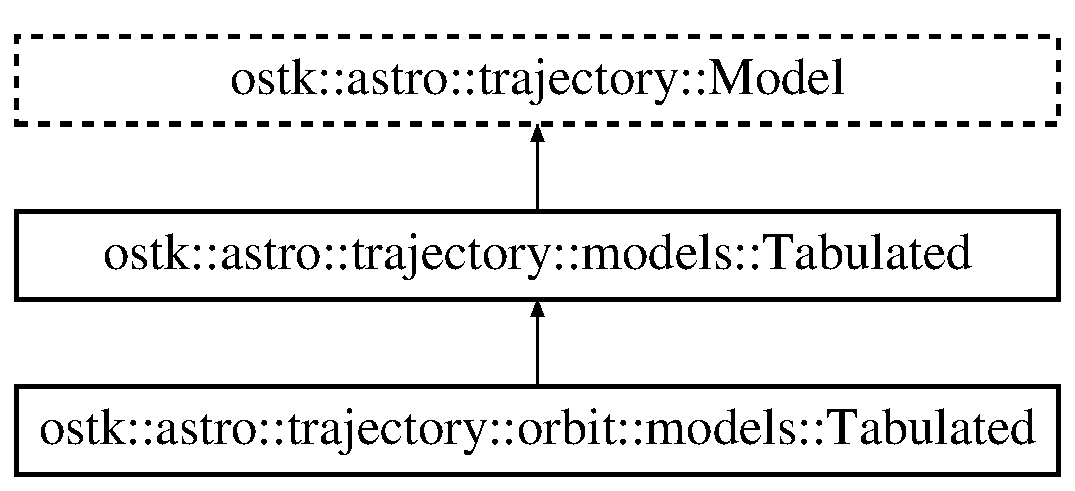
\includegraphics[height=3.000000cm]{classostk_1_1astro_1_1trajectory_1_1models_1_1_tabulated}
\end{center}
\end{figure}
\doxysubsection*{Public Types}
\begin{DoxyCompactItemize}
\item 
enum \mbox{\hyperlink{classostk_1_1astro_1_1trajectory_1_1models_1_1_tabulated_a6cfa3365af2959f1e2b966aeaa7d4d77}{Interpolation\+Type}} \{ \mbox{\hyperlink{classostk_1_1astro_1_1trajectory_1_1models_1_1_tabulated_a6cfa3365af2959f1e2b966aeaa7d4d77a32a843da6ea40ab3b17a3421ccdf671b}{Interpolation\+Type\+::\+Linear}}, 
\mbox{\hyperlink{classostk_1_1astro_1_1trajectory_1_1models_1_1_tabulated_a6cfa3365af2959f1e2b966aeaa7d4d77a98cf9ba70112c998166a82b6f289bb9f}{Interpolation\+Type\+::\+Barycentric\+Rational}}, 
\mbox{\hyperlink{classostk_1_1astro_1_1trajectory_1_1models_1_1_tabulated_a6cfa3365af2959f1e2b966aeaa7d4d77abc050383dcd36a2e1f9481e562332cfa}{Interpolation\+Type\+::\+Cubic\+Spline}}
 \}
\end{DoxyCompactItemize}
\doxysubsection*{Public Member Functions}
\begin{DoxyCompactItemize}
\item 
\mbox{\hyperlink{classostk_1_1astro_1_1trajectory_1_1models_1_1_tabulated_a1c9756b91c3ff6508560951098f81acd}{Tabulated}} (const Array$<$ \mbox{\hyperlink{classostk_1_1astro_1_1trajectory_1_1_state}{State}} $>$ \&a\+State\+Array, const \mbox{\hyperlink{classostk_1_1astro_1_1trajectory_1_1models_1_1_tabulated_a6cfa3365af2959f1e2b966aeaa7d4d77}{Interpolation\+Type}} \&an\+Interpolation\+Type=\mbox{\hyperlink{_trajectory_2_models_2_tabulated_8hpp_ad7c40273c493179caae28b4aa810dc29}{D\+E\+F\+A\+U\+L\+T\+\_\+\+T\+A\+B\+U\+L\+A\+T\+E\+D\+\_\+\+I\+N\+T\+E\+R\+P\+O\+L\+A\+T\+I\+O\+N\+\_\+\+T\+Y\+PE}})
\item 
virtual \mbox{\hyperlink{classostk_1_1astro_1_1trajectory_1_1models_1_1_tabulated}{Tabulated}} $\ast$ \mbox{\hyperlink{classostk_1_1astro_1_1trajectory_1_1models_1_1_tabulated_a553d2c4027ce269c1c2b3f4e9c65e14d}{clone}} () const override
\item 
bool \mbox{\hyperlink{classostk_1_1astro_1_1trajectory_1_1models_1_1_tabulated_aec2a2014af9276d9cc89cd1898a5d001}{operator==}} (const \mbox{\hyperlink{classostk_1_1astro_1_1trajectory_1_1models_1_1_tabulated}{Tabulated}} \&a\+Tabulated\+Model) const
\item 
bool \mbox{\hyperlink{classostk_1_1astro_1_1trajectory_1_1models_1_1_tabulated_a4ffc2bdbb107823f39fee423323b12cc}{operator!=}} (const \mbox{\hyperlink{classostk_1_1astro_1_1trajectory_1_1models_1_1_tabulated}{Tabulated}} \&a\+Tabulated\+Model) const
\item 
virtual bool \mbox{\hyperlink{classostk_1_1astro_1_1trajectory_1_1models_1_1_tabulated_a379da4c10a738c3f4578042c9bae0c91}{is\+Defined}} () const override
\item 
Interval \mbox{\hyperlink{classostk_1_1astro_1_1trajectory_1_1models_1_1_tabulated_ad385f1f0126aa00fbc33c120debff086}{get\+Interval}} () const
\item 
\mbox{\hyperlink{classostk_1_1astro_1_1trajectory_1_1models_1_1_tabulated_a6cfa3365af2959f1e2b966aeaa7d4d77}{Interpolation\+Type}} \mbox{\hyperlink{classostk_1_1astro_1_1trajectory_1_1models_1_1_tabulated_a08ee176a9ef597e7176c28f254f55598}{get\+Interpolation\+Type}} () const
\item 
\mbox{\hyperlink{classostk_1_1astro_1_1trajectory_1_1_state}{State}} \mbox{\hyperlink{classostk_1_1astro_1_1trajectory_1_1models_1_1_tabulated_adbc913778b26803ff1343ef80a41707d}{get\+First\+State}} () const
\item 
\mbox{\hyperlink{classostk_1_1astro_1_1trajectory_1_1_state}{State}} \mbox{\hyperlink{classostk_1_1astro_1_1trajectory_1_1models_1_1_tabulated_a7b7b624e62841fb93513f02c9d7c8f67}{get\+Last\+State}} () const
\item 
virtual \mbox{\hyperlink{classostk_1_1astro_1_1trajectory_1_1_state}{State}} \mbox{\hyperlink{classostk_1_1astro_1_1trajectory_1_1models_1_1_tabulated_af2ebaa6456986636aa58c2f8666ed0b9}{calculate\+State\+At}} (const Instant \&an\+Instant) const override
\item 
virtual Array$<$ \mbox{\hyperlink{classostk_1_1astro_1_1trajectory_1_1_state}{State}} $>$ \mbox{\hyperlink{classostk_1_1astro_1_1trajectory_1_1models_1_1_tabulated_a32239d967738b2625504bc5efe8737eb}{calculate\+States\+At}} (const Array$<$ Instant $>$ \&an\+Instant\+Array) const override
\item 
virtual void \mbox{\hyperlink{classostk_1_1astro_1_1trajectory_1_1models_1_1_tabulated_a330bfffa50eb77eb7f6d45cfec1e9e29}{print}} (std\+::ostream \&an\+Output\+Stream, bool display\+Decorator=true) const override
\end{DoxyCompactItemize}
\doxysubsection*{Static Public Member Functions}
\begin{DoxyCompactItemize}
\item 
static \mbox{\hyperlink{classostk_1_1astro_1_1trajectory_1_1models_1_1_tabulated}{Tabulated}} \mbox{\hyperlink{classostk_1_1astro_1_1trajectory_1_1models_1_1_tabulated_a81cf8ebea4354805ab69e732bfe73d77}{Load}} (const File \&a\+File)
\end{DoxyCompactItemize}
\doxysubsection*{Protected Member Functions}
\begin{DoxyCompactItemize}
\item 
virtual bool \mbox{\hyperlink{classostk_1_1astro_1_1trajectory_1_1models_1_1_tabulated_a9d206aee35ebabe4b36ddfc057142f16}{operator==}} (const \mbox{\hyperlink{classostk_1_1astro_1_1trajectory_1_1_model}{Model}} \&a\+Model) const override
\item 
virtual bool \mbox{\hyperlink{classostk_1_1astro_1_1trajectory_1_1models_1_1_tabulated_a5e047165eb79ea50d257c2cb1bafc30d}{operator!=}} (const \mbox{\hyperlink{classostk_1_1astro_1_1trajectory_1_1_model}{Model}} \&a\+Model) const override
\end{DoxyCompactItemize}
\doxysubsection*{Friends}
\begin{DoxyCompactItemize}
\item 
std\+::ostream \& \mbox{\hyperlink{classostk_1_1astro_1_1trajectory_1_1models_1_1_tabulated_af2b779226be02822defbe40cf6d3c4b8}{operator$<$$<$}} (std\+::ostream \&an\+Output\+Stream, const \mbox{\hyperlink{classostk_1_1astro_1_1trajectory_1_1models_1_1_tabulated}{Tabulated}} \&a\+Tabulated\+Model)
\end{DoxyCompactItemize}


\doxysubsection{Detailed Description}
\mbox{\hyperlink{classostk_1_1astro_1_1trajectory_1_1models_1_1_tabulated}{Tabulated}} trajectory model. 

\begin{DoxyVerb}                        Interpolation is performed between states using the specified interpolation scheme.
                        For now, linear, barycentric rational and cubic spline interpolation schemes are
                        supported. 
\end{DoxyVerb}
 

\doxysubsection{Member Enumeration Documentation}
\mbox{\Hypertarget{classostk_1_1astro_1_1trajectory_1_1models_1_1_tabulated_a6cfa3365af2959f1e2b966aeaa7d4d77}\label{classostk_1_1astro_1_1trajectory_1_1models_1_1_tabulated_a6cfa3365af2959f1e2b966aeaa7d4d77}} 
\index{ostk::astro::trajectory::models::Tabulated@{ostk::astro::trajectory::models::Tabulated}!InterpolationType@{InterpolationType}}
\index{InterpolationType@{InterpolationType}!ostk::astro::trajectory::models::Tabulated@{ostk::astro::trajectory::models::Tabulated}}
\doxysubsubsection{\texorpdfstring{InterpolationType}{InterpolationType}}
{\footnotesize\ttfamily enum \mbox{\hyperlink{classostk_1_1astro_1_1trajectory_1_1models_1_1_tabulated_a6cfa3365af2959f1e2b966aeaa7d4d77}{ostk\+::astro\+::trajectory\+::models\+::\+Tabulated\+::\+Interpolation\+Type}}\hspace{0.3cm}{\ttfamily [strong]}}

\begin{DoxyEnumFields}{Enumerator}
\raisebox{\heightof{T}}[0pt][0pt]{\index{Linear@{Linear}!ostk::astro::trajectory::models::Tabulated@{ostk::astro::trajectory::models::Tabulated}}\index{ostk::astro::trajectory::models::Tabulated@{ostk::astro::trajectory::models::Tabulated}!Linear@{Linear}}}\mbox{\Hypertarget{classostk_1_1astro_1_1trajectory_1_1models_1_1_tabulated_a6cfa3365af2959f1e2b966aeaa7d4d77a32a843da6ea40ab3b17a3421ccdf671b}\label{classostk_1_1astro_1_1trajectory_1_1models_1_1_tabulated_a6cfa3365af2959f1e2b966aeaa7d4d77a32a843da6ea40ab3b17a3421ccdf671b}} 
Linear&\\
\hline

\raisebox{\heightof{T}}[0pt][0pt]{\index{BarycentricRational@{BarycentricRational}!ostk::astro::trajectory::models::Tabulated@{ostk::astro::trajectory::models::Tabulated}}\index{ostk::astro::trajectory::models::Tabulated@{ostk::astro::trajectory::models::Tabulated}!BarycentricRational@{BarycentricRational}}}\mbox{\Hypertarget{classostk_1_1astro_1_1trajectory_1_1models_1_1_tabulated_a6cfa3365af2959f1e2b966aeaa7d4d77a98cf9ba70112c998166a82b6f289bb9f}\label{classostk_1_1astro_1_1trajectory_1_1models_1_1_tabulated_a6cfa3365af2959f1e2b966aeaa7d4d77a98cf9ba70112c998166a82b6f289bb9f}} 
Barycentric\+Rational&\\
\hline

\raisebox{\heightof{T}}[0pt][0pt]{\index{CubicSpline@{CubicSpline}!ostk::astro::trajectory::models::Tabulated@{ostk::astro::trajectory::models::Tabulated}}\index{ostk::astro::trajectory::models::Tabulated@{ostk::astro::trajectory::models::Tabulated}!CubicSpline@{CubicSpline}}}\mbox{\Hypertarget{classostk_1_1astro_1_1trajectory_1_1models_1_1_tabulated_a6cfa3365af2959f1e2b966aeaa7d4d77abc050383dcd36a2e1f9481e562332cfa}\label{classostk_1_1astro_1_1trajectory_1_1models_1_1_tabulated_a6cfa3365af2959f1e2b966aeaa7d4d77abc050383dcd36a2e1f9481e562332cfa}} 
Cubic\+Spline&\\
\hline

\end{DoxyEnumFields}


\doxysubsection{Constructor \& Destructor Documentation}
\mbox{\Hypertarget{classostk_1_1astro_1_1trajectory_1_1models_1_1_tabulated_a1c9756b91c3ff6508560951098f81acd}\label{classostk_1_1astro_1_1trajectory_1_1models_1_1_tabulated_a1c9756b91c3ff6508560951098f81acd}} 
\index{ostk::astro::trajectory::models::Tabulated@{ostk::astro::trajectory::models::Tabulated}!Tabulated@{Tabulated}}
\index{Tabulated@{Tabulated}!ostk::astro::trajectory::models::Tabulated@{ostk::astro::trajectory::models::Tabulated}}
\doxysubsubsection{\texorpdfstring{Tabulated()}{Tabulated()}}
{\footnotesize\ttfamily ostk\+::astro\+::trajectory\+::models\+::\+Tabulated\+::\+Tabulated (\begin{DoxyParamCaption}\item[{const Array$<$ \mbox{\hyperlink{classostk_1_1astro_1_1trajectory_1_1_state}{State}} $>$ \&}]{a\+State\+Array,  }\item[{const \mbox{\hyperlink{classostk_1_1astro_1_1trajectory_1_1models_1_1_tabulated_a6cfa3365af2959f1e2b966aeaa7d4d77}{Interpolation\+Type}} \&}]{an\+Interpolation\+Type = {\ttfamily \mbox{\hyperlink{_trajectory_2_models_2_tabulated_8hpp_ad7c40273c493179caae28b4aa810dc29}{D\+E\+F\+A\+U\+L\+T\+\_\+\+T\+A\+B\+U\+L\+A\+T\+E\+D\+\_\+\+I\+N\+T\+E\+R\+P\+O\+L\+A\+T\+I\+O\+N\+\_\+\+T\+Y\+PE}}} }\end{DoxyParamCaption})}



\doxysubsection{Member Function Documentation}
\mbox{\Hypertarget{classostk_1_1astro_1_1trajectory_1_1models_1_1_tabulated_af2ebaa6456986636aa58c2f8666ed0b9}\label{classostk_1_1astro_1_1trajectory_1_1models_1_1_tabulated_af2ebaa6456986636aa58c2f8666ed0b9}} 
\index{ostk::astro::trajectory::models::Tabulated@{ostk::astro::trajectory::models::Tabulated}!calculateStateAt@{calculateStateAt}}
\index{calculateStateAt@{calculateStateAt}!ostk::astro::trajectory::models::Tabulated@{ostk::astro::trajectory::models::Tabulated}}
\doxysubsubsection{\texorpdfstring{calculateStateAt()}{calculateStateAt()}}
{\footnotesize\ttfamily \mbox{\hyperlink{classostk_1_1astro_1_1trajectory_1_1_state}{State}} ostk\+::astro\+::trajectory\+::models\+::\+Tabulated\+::calculate\+State\+At (\begin{DoxyParamCaption}\item[{const Instant \&}]{an\+Instant }\end{DoxyParamCaption}) const\hspace{0.3cm}{\ttfamily [override]}, {\ttfamily [virtual]}}



Implements \mbox{\hyperlink{classostk_1_1astro_1_1trajectory_1_1_model_ad25eeaded2946bf73d44161b5f4e9a0e}{ostk\+::astro\+::trajectory\+::\+Model}}.



Reimplemented in \mbox{\hyperlink{classostk_1_1astro_1_1trajectory_1_1orbit_1_1models_1_1_tabulated_ad7935cafe71b572b97b9df93e469d2f8}{ostk\+::astro\+::trajectory\+::orbit\+::models\+::\+Tabulated}}.

\mbox{\Hypertarget{classostk_1_1astro_1_1trajectory_1_1models_1_1_tabulated_a32239d967738b2625504bc5efe8737eb}\label{classostk_1_1astro_1_1trajectory_1_1models_1_1_tabulated_a32239d967738b2625504bc5efe8737eb}} 
\index{ostk::astro::trajectory::models::Tabulated@{ostk::astro::trajectory::models::Tabulated}!calculateStatesAt@{calculateStatesAt}}
\index{calculateStatesAt@{calculateStatesAt}!ostk::astro::trajectory::models::Tabulated@{ostk::astro::trajectory::models::Tabulated}}
\doxysubsubsection{\texorpdfstring{calculateStatesAt()}{calculateStatesAt()}}
{\footnotesize\ttfamily Array$<$ \mbox{\hyperlink{classostk_1_1astro_1_1trajectory_1_1_state}{State}} $>$ ostk\+::astro\+::trajectory\+::models\+::\+Tabulated\+::calculate\+States\+At (\begin{DoxyParamCaption}\item[{const Array$<$ Instant $>$ \&}]{an\+Instant\+Array }\end{DoxyParamCaption}) const\hspace{0.3cm}{\ttfamily [override]}, {\ttfamily [virtual]}}



Reimplemented from \mbox{\hyperlink{classostk_1_1astro_1_1trajectory_1_1_model_a3c3e4913aed2272174c0e6cd0d1a6415}{ostk\+::astro\+::trajectory\+::\+Model}}.

\mbox{\Hypertarget{classostk_1_1astro_1_1trajectory_1_1models_1_1_tabulated_a553d2c4027ce269c1c2b3f4e9c65e14d}\label{classostk_1_1astro_1_1trajectory_1_1models_1_1_tabulated_a553d2c4027ce269c1c2b3f4e9c65e14d}} 
\index{ostk::astro::trajectory::models::Tabulated@{ostk::astro::trajectory::models::Tabulated}!clone@{clone}}
\index{clone@{clone}!ostk::astro::trajectory::models::Tabulated@{ostk::astro::trajectory::models::Tabulated}}
\doxysubsubsection{\texorpdfstring{clone()}{clone()}}
{\footnotesize\ttfamily \mbox{\hyperlink{classostk_1_1astro_1_1trajectory_1_1models_1_1_tabulated}{Tabulated}} $\ast$ ostk\+::astro\+::trajectory\+::models\+::\+Tabulated\+::clone (\begin{DoxyParamCaption}{ }\end{DoxyParamCaption}) const\hspace{0.3cm}{\ttfamily [override]}, {\ttfamily [virtual]}}



Implements \mbox{\hyperlink{classostk_1_1astro_1_1trajectory_1_1_model_ad9f1467f711b07796ddc1437fb9ad9df}{ostk\+::astro\+::trajectory\+::\+Model}}.



Reimplemented in \mbox{\hyperlink{classostk_1_1astro_1_1trajectory_1_1orbit_1_1models_1_1_tabulated_a53603727c33f9ff8db520831cf666142}{ostk\+::astro\+::trajectory\+::orbit\+::models\+::\+Tabulated}}.

\mbox{\Hypertarget{classostk_1_1astro_1_1trajectory_1_1models_1_1_tabulated_adbc913778b26803ff1343ef80a41707d}\label{classostk_1_1astro_1_1trajectory_1_1models_1_1_tabulated_adbc913778b26803ff1343ef80a41707d}} 
\index{ostk::astro::trajectory::models::Tabulated@{ostk::astro::trajectory::models::Tabulated}!getFirstState@{getFirstState}}
\index{getFirstState@{getFirstState}!ostk::astro::trajectory::models::Tabulated@{ostk::astro::trajectory::models::Tabulated}}
\doxysubsubsection{\texorpdfstring{getFirstState()}{getFirstState()}}
{\footnotesize\ttfamily \mbox{\hyperlink{classostk_1_1astro_1_1trajectory_1_1_state}{State}} ostk\+::astro\+::trajectory\+::models\+::\+Tabulated\+::get\+First\+State (\begin{DoxyParamCaption}{ }\end{DoxyParamCaption}) const}

\mbox{\Hypertarget{classostk_1_1astro_1_1trajectory_1_1models_1_1_tabulated_a08ee176a9ef597e7176c28f254f55598}\label{classostk_1_1astro_1_1trajectory_1_1models_1_1_tabulated_a08ee176a9ef597e7176c28f254f55598}} 
\index{ostk::astro::trajectory::models::Tabulated@{ostk::astro::trajectory::models::Tabulated}!getInterpolationType@{getInterpolationType}}
\index{getInterpolationType@{getInterpolationType}!ostk::astro::trajectory::models::Tabulated@{ostk::astro::trajectory::models::Tabulated}}
\doxysubsubsection{\texorpdfstring{getInterpolationType()}{getInterpolationType()}}
{\footnotesize\ttfamily \mbox{\hyperlink{classostk_1_1astro_1_1trajectory_1_1models_1_1_tabulated_a6cfa3365af2959f1e2b966aeaa7d4d77}{Tabulated\+::\+Interpolation\+Type}} ostk\+::astro\+::trajectory\+::models\+::\+Tabulated\+::get\+Interpolation\+Type (\begin{DoxyParamCaption}{ }\end{DoxyParamCaption}) const}

\mbox{\Hypertarget{classostk_1_1astro_1_1trajectory_1_1models_1_1_tabulated_ad385f1f0126aa00fbc33c120debff086}\label{classostk_1_1astro_1_1trajectory_1_1models_1_1_tabulated_ad385f1f0126aa00fbc33c120debff086}} 
\index{ostk::astro::trajectory::models::Tabulated@{ostk::astro::trajectory::models::Tabulated}!getInterval@{getInterval}}
\index{getInterval@{getInterval}!ostk::astro::trajectory::models::Tabulated@{ostk::astro::trajectory::models::Tabulated}}
\doxysubsubsection{\texorpdfstring{getInterval()}{getInterval()}}
{\footnotesize\ttfamily Interval ostk\+::astro\+::trajectory\+::models\+::\+Tabulated\+::get\+Interval (\begin{DoxyParamCaption}{ }\end{DoxyParamCaption}) const}

\mbox{\Hypertarget{classostk_1_1astro_1_1trajectory_1_1models_1_1_tabulated_a7b7b624e62841fb93513f02c9d7c8f67}\label{classostk_1_1astro_1_1trajectory_1_1models_1_1_tabulated_a7b7b624e62841fb93513f02c9d7c8f67}} 
\index{ostk::astro::trajectory::models::Tabulated@{ostk::astro::trajectory::models::Tabulated}!getLastState@{getLastState}}
\index{getLastState@{getLastState}!ostk::astro::trajectory::models::Tabulated@{ostk::astro::trajectory::models::Tabulated}}
\doxysubsubsection{\texorpdfstring{getLastState()}{getLastState()}}
{\footnotesize\ttfamily \mbox{\hyperlink{classostk_1_1astro_1_1trajectory_1_1_state}{State}} ostk\+::astro\+::trajectory\+::models\+::\+Tabulated\+::get\+Last\+State (\begin{DoxyParamCaption}{ }\end{DoxyParamCaption}) const}

\mbox{\Hypertarget{classostk_1_1astro_1_1trajectory_1_1models_1_1_tabulated_a379da4c10a738c3f4578042c9bae0c91}\label{classostk_1_1astro_1_1trajectory_1_1models_1_1_tabulated_a379da4c10a738c3f4578042c9bae0c91}} 
\index{ostk::astro::trajectory::models::Tabulated@{ostk::astro::trajectory::models::Tabulated}!isDefined@{isDefined}}
\index{isDefined@{isDefined}!ostk::astro::trajectory::models::Tabulated@{ostk::astro::trajectory::models::Tabulated}}
\doxysubsubsection{\texorpdfstring{isDefined()}{isDefined()}}
{\footnotesize\ttfamily bool ostk\+::astro\+::trajectory\+::models\+::\+Tabulated\+::is\+Defined (\begin{DoxyParamCaption}{ }\end{DoxyParamCaption}) const\hspace{0.3cm}{\ttfamily [override]}, {\ttfamily [virtual]}}



Implements \mbox{\hyperlink{classostk_1_1astro_1_1trajectory_1_1_model_a0d5cf6f754905f06c0ec1e39618c20a1}{ostk\+::astro\+::trajectory\+::\+Model}}.



Reimplemented in \mbox{\hyperlink{classostk_1_1astro_1_1trajectory_1_1orbit_1_1models_1_1_tabulated_ad114ba4762b54211f74f0aa3ac5eedae}{ostk\+::astro\+::trajectory\+::orbit\+::models\+::\+Tabulated}}.

\mbox{\Hypertarget{classostk_1_1astro_1_1trajectory_1_1models_1_1_tabulated_a81cf8ebea4354805ab69e732bfe73d77}\label{classostk_1_1astro_1_1trajectory_1_1models_1_1_tabulated_a81cf8ebea4354805ab69e732bfe73d77}} 
\index{ostk::astro::trajectory::models::Tabulated@{ostk::astro::trajectory::models::Tabulated}!Load@{Load}}
\index{Load@{Load}!ostk::astro::trajectory::models::Tabulated@{ostk::astro::trajectory::models::Tabulated}}
\doxysubsubsection{\texorpdfstring{Load()}{Load()}}
{\footnotesize\ttfamily static \mbox{\hyperlink{classostk_1_1astro_1_1trajectory_1_1models_1_1_tabulated}{Tabulated}} ostk\+::astro\+::trajectory\+::models\+::\+Tabulated\+::\+Load (\begin{DoxyParamCaption}\item[{const File \&}]{a\+File }\end{DoxyParamCaption})\hspace{0.3cm}{\ttfamily [static]}}

\mbox{\Hypertarget{classostk_1_1astro_1_1trajectory_1_1models_1_1_tabulated_a5e047165eb79ea50d257c2cb1bafc30d}\label{classostk_1_1astro_1_1trajectory_1_1models_1_1_tabulated_a5e047165eb79ea50d257c2cb1bafc30d}} 
\index{ostk::astro::trajectory::models::Tabulated@{ostk::astro::trajectory::models::Tabulated}!operator"!=@{operator"!=}}
\index{operator"!=@{operator"!=}!ostk::astro::trajectory::models::Tabulated@{ostk::astro::trajectory::models::Tabulated}}
\doxysubsubsection{\texorpdfstring{operator"!=()}{operator!=()}\hspace{0.1cm}{\footnotesize\ttfamily [1/2]}}
{\footnotesize\ttfamily bool ostk\+::astro\+::trajectory\+::models\+::\+Tabulated\+::operator!= (\begin{DoxyParamCaption}\item[{const \mbox{\hyperlink{classostk_1_1astro_1_1trajectory_1_1_model}{Model}} \&}]{a\+Model }\end{DoxyParamCaption}) const\hspace{0.3cm}{\ttfamily [override]}, {\ttfamily [protected]}, {\ttfamily [virtual]}}



Implements \mbox{\hyperlink{classostk_1_1astro_1_1trajectory_1_1_model_a2dd77b9f6939d738f3a489f26c955340}{ostk\+::astro\+::trajectory\+::\+Model}}.



Reimplemented in \mbox{\hyperlink{classostk_1_1astro_1_1trajectory_1_1orbit_1_1models_1_1_tabulated_a17610dc24fefecd03ae595cc78ef3079}{ostk\+::astro\+::trajectory\+::orbit\+::models\+::\+Tabulated}}.

\mbox{\Hypertarget{classostk_1_1astro_1_1trajectory_1_1models_1_1_tabulated_a4ffc2bdbb107823f39fee423323b12cc}\label{classostk_1_1astro_1_1trajectory_1_1models_1_1_tabulated_a4ffc2bdbb107823f39fee423323b12cc}} 
\index{ostk::astro::trajectory::models::Tabulated@{ostk::astro::trajectory::models::Tabulated}!operator"!=@{operator"!=}}
\index{operator"!=@{operator"!=}!ostk::astro::trajectory::models::Tabulated@{ostk::astro::trajectory::models::Tabulated}}
\doxysubsubsection{\texorpdfstring{operator"!=()}{operator!=()}\hspace{0.1cm}{\footnotesize\ttfamily [2/2]}}
{\footnotesize\ttfamily bool ostk\+::astro\+::trajectory\+::models\+::\+Tabulated\+::operator!= (\begin{DoxyParamCaption}\item[{const \mbox{\hyperlink{classostk_1_1astro_1_1trajectory_1_1models_1_1_tabulated}{Tabulated}} \&}]{a\+Tabulated\+Model }\end{DoxyParamCaption}) const}

\mbox{\Hypertarget{classostk_1_1astro_1_1trajectory_1_1models_1_1_tabulated_a9d206aee35ebabe4b36ddfc057142f16}\label{classostk_1_1astro_1_1trajectory_1_1models_1_1_tabulated_a9d206aee35ebabe4b36ddfc057142f16}} 
\index{ostk::astro::trajectory::models::Tabulated@{ostk::astro::trajectory::models::Tabulated}!operator==@{operator==}}
\index{operator==@{operator==}!ostk::astro::trajectory::models::Tabulated@{ostk::astro::trajectory::models::Tabulated}}
\doxysubsubsection{\texorpdfstring{operator==()}{operator==()}\hspace{0.1cm}{\footnotesize\ttfamily [1/2]}}
{\footnotesize\ttfamily bool ostk\+::astro\+::trajectory\+::models\+::\+Tabulated\+::operator== (\begin{DoxyParamCaption}\item[{const \mbox{\hyperlink{classostk_1_1astro_1_1trajectory_1_1_model}{Model}} \&}]{a\+Model }\end{DoxyParamCaption}) const\hspace{0.3cm}{\ttfamily [override]}, {\ttfamily [protected]}, {\ttfamily [virtual]}}



Implements \mbox{\hyperlink{classostk_1_1astro_1_1trajectory_1_1_model_a874f79846e845859c070ce1b9874fc9c}{ostk\+::astro\+::trajectory\+::\+Model}}.



Reimplemented in \mbox{\hyperlink{classostk_1_1astro_1_1trajectory_1_1orbit_1_1models_1_1_tabulated_abd72010cb413d8479c097376bfebaf56}{ostk\+::astro\+::trajectory\+::orbit\+::models\+::\+Tabulated}}.

\mbox{\Hypertarget{classostk_1_1astro_1_1trajectory_1_1models_1_1_tabulated_aec2a2014af9276d9cc89cd1898a5d001}\label{classostk_1_1astro_1_1trajectory_1_1models_1_1_tabulated_aec2a2014af9276d9cc89cd1898a5d001}} 
\index{ostk::astro::trajectory::models::Tabulated@{ostk::astro::trajectory::models::Tabulated}!operator==@{operator==}}
\index{operator==@{operator==}!ostk::astro::trajectory::models::Tabulated@{ostk::astro::trajectory::models::Tabulated}}
\doxysubsubsection{\texorpdfstring{operator==()}{operator==()}\hspace{0.1cm}{\footnotesize\ttfamily [2/2]}}
{\footnotesize\ttfamily bool ostk\+::astro\+::trajectory\+::models\+::\+Tabulated\+::operator== (\begin{DoxyParamCaption}\item[{const \mbox{\hyperlink{classostk_1_1astro_1_1trajectory_1_1models_1_1_tabulated}{Tabulated}} \&}]{a\+Tabulated\+Model }\end{DoxyParamCaption}) const}

\mbox{\Hypertarget{classostk_1_1astro_1_1trajectory_1_1models_1_1_tabulated_a330bfffa50eb77eb7f6d45cfec1e9e29}\label{classostk_1_1astro_1_1trajectory_1_1models_1_1_tabulated_a330bfffa50eb77eb7f6d45cfec1e9e29}} 
\index{ostk::astro::trajectory::models::Tabulated@{ostk::astro::trajectory::models::Tabulated}!print@{print}}
\index{print@{print}!ostk::astro::trajectory::models::Tabulated@{ostk::astro::trajectory::models::Tabulated}}
\doxysubsubsection{\texorpdfstring{print()}{print()}}
{\footnotesize\ttfamily void ostk\+::astro\+::trajectory\+::models\+::\+Tabulated\+::print (\begin{DoxyParamCaption}\item[{std\+::ostream \&}]{an\+Output\+Stream,  }\item[{bool}]{display\+Decorator = {\ttfamily true} }\end{DoxyParamCaption}) const\hspace{0.3cm}{\ttfamily [override]}, {\ttfamily [virtual]}}



Implements \mbox{\hyperlink{classostk_1_1astro_1_1trajectory_1_1_model_a4b2098483430a820481ed50b81656e31}{ostk\+::astro\+::trajectory\+::\+Model}}.



Reimplemented in \mbox{\hyperlink{classostk_1_1astro_1_1trajectory_1_1orbit_1_1models_1_1_tabulated_a66be3f1f23a464c666c38a3adcc3bab5}{ostk\+::astro\+::trajectory\+::orbit\+::models\+::\+Tabulated}}.



\doxysubsection{Friends And Related Function Documentation}
\mbox{\Hypertarget{classostk_1_1astro_1_1trajectory_1_1models_1_1_tabulated_af2b779226be02822defbe40cf6d3c4b8}\label{classostk_1_1astro_1_1trajectory_1_1models_1_1_tabulated_af2b779226be02822defbe40cf6d3c4b8}} 
\index{ostk::astro::trajectory::models::Tabulated@{ostk::astro::trajectory::models::Tabulated}!operator$<$$<$@{operator$<$$<$}}
\index{operator$<$$<$@{operator$<$$<$}!ostk::astro::trajectory::models::Tabulated@{ostk::astro::trajectory::models::Tabulated}}
\doxysubsubsection{\texorpdfstring{operator$<$$<$}{operator<<}}
{\footnotesize\ttfamily std\+::ostream\& operator$<$$<$ (\begin{DoxyParamCaption}\item[{std\+::ostream \&}]{an\+Output\+Stream,  }\item[{const \mbox{\hyperlink{classostk_1_1astro_1_1trajectory_1_1models_1_1_tabulated}{Tabulated}} \&}]{a\+Tabulated\+Model }\end{DoxyParamCaption})\hspace{0.3cm}{\ttfamily [friend]}}



The documentation for this class was generated from the following files\+:\begin{DoxyCompactItemize}
\item 
include/\+Open\+Space\+Toolkit/\+Astrodynamics/\+Trajectory/\+Models/\mbox{\hyperlink{_trajectory_2_models_2_tabulated_8hpp}{Tabulated.\+hpp}}\item 
src/\+Open\+Space\+Toolkit/\+Astrodynamics/\+Trajectory/\+Models/\mbox{\hyperlink{_trajectory_2_models_2_tabulated_8cpp}{Tabulated.\+cpp}}\end{DoxyCompactItemize}

\hypertarget{classostk_1_1astro_1_1trajectory_1_1orbit_1_1models_1_1_tabulated}{}\doxysection{ostk\+::astro\+::trajectory\+::orbit\+::models\+::Tabulated Class Reference}
\label{classostk_1_1astro_1_1trajectory_1_1orbit_1_1models_1_1_tabulated}\index{ostk::astro::trajectory::orbit::models::Tabulated@{ostk::astro::trajectory::orbit::models::Tabulated}}


{\ttfamily \#include $<$Tabulated.\+hpp$>$}

Inheritance diagram for ostk\+::astro\+::trajectory\+::orbit\+::models\+::Tabulated\+:\begin{figure}[H]
\begin{center}
\leavevmode
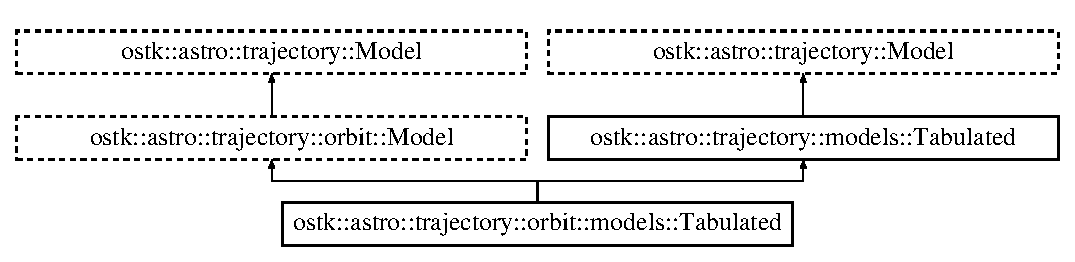
\includegraphics[height=3.000000cm]{classostk_1_1astro_1_1trajectory_1_1orbit_1_1models_1_1_tabulated}
\end{center}
\end{figure}
\doxysubsection*{Public Member Functions}
\begin{DoxyCompactItemize}
\item 
\mbox{\hyperlink{classostk_1_1astro_1_1trajectory_1_1orbit_1_1models_1_1_tabulated_aee7a0780a163332e41338e7176da97df}{Tabulated}} (const Array$<$ \mbox{\hyperlink{classostk_1_1astro_1_1trajectory_1_1_state}{State}} $>$ \&a\+State\+Array, const Integer \&an\+Initial\+Revolution\+Number)
\item 
virtual \mbox{\hyperlink{classostk_1_1astro_1_1trajectory_1_1orbit_1_1models_1_1_tabulated}{Tabulated}} $\ast$ \mbox{\hyperlink{classostk_1_1astro_1_1trajectory_1_1orbit_1_1models_1_1_tabulated_a53603727c33f9ff8db520831cf666142}{clone}} () const override
\item 
bool \mbox{\hyperlink{classostk_1_1astro_1_1trajectory_1_1orbit_1_1models_1_1_tabulated_a43b91c2c968fe65dee1a64bd3c1cdf3f}{operator==}} (const \mbox{\hyperlink{classostk_1_1astro_1_1trajectory_1_1orbit_1_1models_1_1_tabulated}{Tabulated}} \&a\+Tabulated\+Model) const
\item 
bool \mbox{\hyperlink{classostk_1_1astro_1_1trajectory_1_1orbit_1_1models_1_1_tabulated_ab50e1a3858fa4bedf4577e8d9fc30744}{operator!=}} (const \mbox{\hyperlink{classostk_1_1astro_1_1trajectory_1_1orbit_1_1models_1_1_tabulated}{Tabulated}} \&a\+Tabulated\+Model) const
\item 
virtual bool \mbox{\hyperlink{classostk_1_1astro_1_1trajectory_1_1orbit_1_1models_1_1_tabulated_ad114ba4762b54211f74f0aa3ac5eedae}{is\+Defined}} () const override
\item 
virtual Instant \mbox{\hyperlink{classostk_1_1astro_1_1trajectory_1_1orbit_1_1models_1_1_tabulated_a0e92ebaac60e5113989eaadc66062b75}{get\+Epoch}} () const override
\item 
virtual Integer \mbox{\hyperlink{classostk_1_1astro_1_1trajectory_1_1orbit_1_1models_1_1_tabulated_adbd37f167e43cedcb15358c16d62bae8}{get\+Revolution\+Number\+At\+Epoch}} () const override
\item 
virtual \mbox{\hyperlink{classostk_1_1astro_1_1trajectory_1_1_state}{State}} \mbox{\hyperlink{classostk_1_1astro_1_1trajectory_1_1orbit_1_1models_1_1_tabulated_ad7935cafe71b572b97b9df93e469d2f8}{calculate\+State\+At}} (const Instant \&an\+Instant) const override
\item 
virtual Integer \mbox{\hyperlink{classostk_1_1astro_1_1trajectory_1_1orbit_1_1models_1_1_tabulated_ad7aabd8943ffaa16e569e331bdfa414e}{calculate\+Revolution\+Number\+At}} (const Instant \&an\+Instant) const override
\item 
virtual void \mbox{\hyperlink{classostk_1_1astro_1_1trajectory_1_1orbit_1_1models_1_1_tabulated_a66be3f1f23a464c666c38a3adcc3bab5}{print}} (std\+::ostream \&an\+Output\+Stream, bool display\+Decorator) const override
\end{DoxyCompactItemize}
\doxysubsection*{Protected Member Functions}
\begin{DoxyCompactItemize}
\item 
virtual bool \mbox{\hyperlink{classostk_1_1astro_1_1trajectory_1_1orbit_1_1models_1_1_tabulated_abd72010cb413d8479c097376bfebaf56}{operator==}} (const \mbox{\hyperlink{classostk_1_1astro_1_1trajectory_1_1_model}{trajectory\+::\+Model}} \&a\+Model) const override
\item 
virtual bool \mbox{\hyperlink{classostk_1_1astro_1_1trajectory_1_1orbit_1_1models_1_1_tabulated_a17610dc24fefecd03ae595cc78ef3079}{operator!=}} (const \mbox{\hyperlink{classostk_1_1astro_1_1trajectory_1_1_model}{trajectory\+::\+Model}} \&a\+Model) const override
\end{DoxyCompactItemize}
\doxysubsection*{Additional Inherited Members}


\doxysubsection{Constructor \& Destructor Documentation}
\mbox{\Hypertarget{classostk_1_1astro_1_1trajectory_1_1orbit_1_1models_1_1_tabulated_aee7a0780a163332e41338e7176da97df}\label{classostk_1_1astro_1_1trajectory_1_1orbit_1_1models_1_1_tabulated_aee7a0780a163332e41338e7176da97df}} 
\index{ostk::astro::trajectory::orbit::models::Tabulated@{ostk::astro::trajectory::orbit::models::Tabulated}!Tabulated@{Tabulated}}
\index{Tabulated@{Tabulated}!ostk::astro::trajectory::orbit::models::Tabulated@{ostk::astro::trajectory::orbit::models::Tabulated}}
\doxysubsubsection{\texorpdfstring{Tabulated()}{Tabulated()}}
{\footnotesize\ttfamily ostk\+::astro\+::trajectory\+::orbit\+::models\+::\+Tabulated\+::\+Tabulated (\begin{DoxyParamCaption}\item[{const Array$<$ \mbox{\hyperlink{classostk_1_1astro_1_1trajectory_1_1_state}{State}} $>$ \&}]{a\+State\+Array,  }\item[{const Integer \&}]{an\+Initial\+Revolution\+Number }\end{DoxyParamCaption})}



\doxysubsection{Member Function Documentation}
\mbox{\Hypertarget{classostk_1_1astro_1_1trajectory_1_1orbit_1_1models_1_1_tabulated_ad7aabd8943ffaa16e569e331bdfa414e}\label{classostk_1_1astro_1_1trajectory_1_1orbit_1_1models_1_1_tabulated_ad7aabd8943ffaa16e569e331bdfa414e}} 
\index{ostk::astro::trajectory::orbit::models::Tabulated@{ostk::astro::trajectory::orbit::models::Tabulated}!calculateRevolutionNumberAt@{calculateRevolutionNumberAt}}
\index{calculateRevolutionNumberAt@{calculateRevolutionNumberAt}!ostk::astro::trajectory::orbit::models::Tabulated@{ostk::astro::trajectory::orbit::models::Tabulated}}
\doxysubsubsection{\texorpdfstring{calculateRevolutionNumberAt()}{calculateRevolutionNumberAt()}}
{\footnotesize\ttfamily Integer ostk\+::astro\+::trajectory\+::orbit\+::models\+::\+Tabulated\+::calculate\+Revolution\+Number\+At (\begin{DoxyParamCaption}\item[{const Instant \&}]{an\+Instant }\end{DoxyParamCaption}) const\hspace{0.3cm}{\ttfamily [override]}, {\ttfamily [virtual]}}



Implements \mbox{\hyperlink{classostk_1_1astro_1_1trajectory_1_1orbit_1_1_model_aeecf4cc22fa9c766801936c468cc52ac}{ostk\+::astro\+::trajectory\+::orbit\+::\+Model}}.

\mbox{\Hypertarget{classostk_1_1astro_1_1trajectory_1_1orbit_1_1models_1_1_tabulated_ad7935cafe71b572b97b9df93e469d2f8}\label{classostk_1_1astro_1_1trajectory_1_1orbit_1_1models_1_1_tabulated_ad7935cafe71b572b97b9df93e469d2f8}} 
\index{ostk::astro::trajectory::orbit::models::Tabulated@{ostk::astro::trajectory::orbit::models::Tabulated}!calculateStateAt@{calculateStateAt}}
\index{calculateStateAt@{calculateStateAt}!ostk::astro::trajectory::orbit::models::Tabulated@{ostk::astro::trajectory::orbit::models::Tabulated}}
\doxysubsubsection{\texorpdfstring{calculateStateAt()}{calculateStateAt()}}
{\footnotesize\ttfamily \mbox{\hyperlink{classostk_1_1astro_1_1trajectory_1_1_state}{State}} ostk\+::astro\+::trajectory\+::orbit\+::models\+::\+Tabulated\+::calculate\+State\+At (\begin{DoxyParamCaption}\item[{const Instant \&}]{an\+Instant }\end{DoxyParamCaption}) const\hspace{0.3cm}{\ttfamily [override]}, {\ttfamily [virtual]}}



Reimplemented from \mbox{\hyperlink{classostk_1_1astro_1_1trajectory_1_1models_1_1_tabulated_af2ebaa6456986636aa58c2f8666ed0b9}{ostk\+::astro\+::trajectory\+::models\+::\+Tabulated}}.

\mbox{\Hypertarget{classostk_1_1astro_1_1trajectory_1_1orbit_1_1models_1_1_tabulated_a53603727c33f9ff8db520831cf666142}\label{classostk_1_1astro_1_1trajectory_1_1orbit_1_1models_1_1_tabulated_a53603727c33f9ff8db520831cf666142}} 
\index{ostk::astro::trajectory::orbit::models::Tabulated@{ostk::astro::trajectory::orbit::models::Tabulated}!clone@{clone}}
\index{clone@{clone}!ostk::astro::trajectory::orbit::models::Tabulated@{ostk::astro::trajectory::orbit::models::Tabulated}}
\doxysubsubsection{\texorpdfstring{clone()}{clone()}}
{\footnotesize\ttfamily \mbox{\hyperlink{classostk_1_1astro_1_1trajectory_1_1orbit_1_1models_1_1_tabulated}{Tabulated}} $\ast$ ostk\+::astro\+::trajectory\+::orbit\+::models\+::\+Tabulated\+::clone (\begin{DoxyParamCaption}{ }\end{DoxyParamCaption}) const\hspace{0.3cm}{\ttfamily [override]}, {\ttfamily [virtual]}}



Reimplemented from \mbox{\hyperlink{classostk_1_1astro_1_1trajectory_1_1models_1_1_tabulated_a553d2c4027ce269c1c2b3f4e9c65e14d}{ostk\+::astro\+::trajectory\+::models\+::\+Tabulated}}.

\mbox{\Hypertarget{classostk_1_1astro_1_1trajectory_1_1orbit_1_1models_1_1_tabulated_a0e92ebaac60e5113989eaadc66062b75}\label{classostk_1_1astro_1_1trajectory_1_1orbit_1_1models_1_1_tabulated_a0e92ebaac60e5113989eaadc66062b75}} 
\index{ostk::astro::trajectory::orbit::models::Tabulated@{ostk::astro::trajectory::orbit::models::Tabulated}!getEpoch@{getEpoch}}
\index{getEpoch@{getEpoch}!ostk::astro::trajectory::orbit::models::Tabulated@{ostk::astro::trajectory::orbit::models::Tabulated}}
\doxysubsubsection{\texorpdfstring{getEpoch()}{getEpoch()}}
{\footnotesize\ttfamily Instant ostk\+::astro\+::trajectory\+::orbit\+::models\+::\+Tabulated\+::get\+Epoch (\begin{DoxyParamCaption}{ }\end{DoxyParamCaption}) const\hspace{0.3cm}{\ttfamily [override]}, {\ttfamily [virtual]}}



Implements \mbox{\hyperlink{classostk_1_1astro_1_1trajectory_1_1orbit_1_1_model_a22055d5ab4c22e6177a3ddb8f45f1f9b}{ostk\+::astro\+::trajectory\+::orbit\+::\+Model}}.

\mbox{\Hypertarget{classostk_1_1astro_1_1trajectory_1_1orbit_1_1models_1_1_tabulated_adbd37f167e43cedcb15358c16d62bae8}\label{classostk_1_1astro_1_1trajectory_1_1orbit_1_1models_1_1_tabulated_adbd37f167e43cedcb15358c16d62bae8}} 
\index{ostk::astro::trajectory::orbit::models::Tabulated@{ostk::astro::trajectory::orbit::models::Tabulated}!getRevolutionNumberAtEpoch@{getRevolutionNumberAtEpoch}}
\index{getRevolutionNumberAtEpoch@{getRevolutionNumberAtEpoch}!ostk::astro::trajectory::orbit::models::Tabulated@{ostk::astro::trajectory::orbit::models::Tabulated}}
\doxysubsubsection{\texorpdfstring{getRevolutionNumberAtEpoch()}{getRevolutionNumberAtEpoch()}}
{\footnotesize\ttfamily Integer ostk\+::astro\+::trajectory\+::orbit\+::models\+::\+Tabulated\+::get\+Revolution\+Number\+At\+Epoch (\begin{DoxyParamCaption}{ }\end{DoxyParamCaption}) const\hspace{0.3cm}{\ttfamily [override]}, {\ttfamily [virtual]}}



Implements \mbox{\hyperlink{classostk_1_1astro_1_1trajectory_1_1orbit_1_1_model_af3f1866f86045da2c05efe4165735cf4}{ostk\+::astro\+::trajectory\+::orbit\+::\+Model}}.

\mbox{\Hypertarget{classostk_1_1astro_1_1trajectory_1_1orbit_1_1models_1_1_tabulated_ad114ba4762b54211f74f0aa3ac5eedae}\label{classostk_1_1astro_1_1trajectory_1_1orbit_1_1models_1_1_tabulated_ad114ba4762b54211f74f0aa3ac5eedae}} 
\index{ostk::astro::trajectory::orbit::models::Tabulated@{ostk::astro::trajectory::orbit::models::Tabulated}!isDefined@{isDefined}}
\index{isDefined@{isDefined}!ostk::astro::trajectory::orbit::models::Tabulated@{ostk::astro::trajectory::orbit::models::Tabulated}}
\doxysubsubsection{\texorpdfstring{isDefined()}{isDefined()}}
{\footnotesize\ttfamily bool ostk\+::astro\+::trajectory\+::orbit\+::models\+::\+Tabulated\+::is\+Defined (\begin{DoxyParamCaption}{ }\end{DoxyParamCaption}) const\hspace{0.3cm}{\ttfamily [override]}, {\ttfamily [virtual]}}



Reimplemented from \mbox{\hyperlink{classostk_1_1astro_1_1trajectory_1_1models_1_1_tabulated_a379da4c10a738c3f4578042c9bae0c91}{ostk\+::astro\+::trajectory\+::models\+::\+Tabulated}}.

\mbox{\Hypertarget{classostk_1_1astro_1_1trajectory_1_1orbit_1_1models_1_1_tabulated_ab50e1a3858fa4bedf4577e8d9fc30744}\label{classostk_1_1astro_1_1trajectory_1_1orbit_1_1models_1_1_tabulated_ab50e1a3858fa4bedf4577e8d9fc30744}} 
\index{ostk::astro::trajectory::orbit::models::Tabulated@{ostk::astro::trajectory::orbit::models::Tabulated}!operator"!=@{operator"!=}}
\index{operator"!=@{operator"!=}!ostk::astro::trajectory::orbit::models::Tabulated@{ostk::astro::trajectory::orbit::models::Tabulated}}
\doxysubsubsection{\texorpdfstring{operator"!=()}{operator!=()}\hspace{0.1cm}{\footnotesize\ttfamily [1/2]}}
{\footnotesize\ttfamily bool ostk\+::astro\+::trajectory\+::orbit\+::models\+::\+Tabulated\+::operator!= (\begin{DoxyParamCaption}\item[{const \mbox{\hyperlink{classostk_1_1astro_1_1trajectory_1_1orbit_1_1models_1_1_tabulated}{Tabulated}} \&}]{a\+Tabulated\+Model }\end{DoxyParamCaption}) const}

\mbox{\Hypertarget{classostk_1_1astro_1_1trajectory_1_1orbit_1_1models_1_1_tabulated_a17610dc24fefecd03ae595cc78ef3079}\label{classostk_1_1astro_1_1trajectory_1_1orbit_1_1models_1_1_tabulated_a17610dc24fefecd03ae595cc78ef3079}} 
\index{ostk::astro::trajectory::orbit::models::Tabulated@{ostk::astro::trajectory::orbit::models::Tabulated}!operator"!=@{operator"!=}}
\index{operator"!=@{operator"!=}!ostk::astro::trajectory::orbit::models::Tabulated@{ostk::astro::trajectory::orbit::models::Tabulated}}
\doxysubsubsection{\texorpdfstring{operator"!=()}{operator!=()}\hspace{0.1cm}{\footnotesize\ttfamily [2/2]}}
{\footnotesize\ttfamily bool ostk\+::astro\+::trajectory\+::orbit\+::models\+::\+Tabulated\+::operator!= (\begin{DoxyParamCaption}\item[{const \mbox{\hyperlink{classostk_1_1astro_1_1trajectory_1_1_model}{trajectory\+::\+Model}} \&}]{a\+Model }\end{DoxyParamCaption}) const\hspace{0.3cm}{\ttfamily [override]}, {\ttfamily [protected]}, {\ttfamily [virtual]}}



Reimplemented from \mbox{\hyperlink{classostk_1_1astro_1_1trajectory_1_1models_1_1_tabulated_a5e047165eb79ea50d257c2cb1bafc30d}{ostk\+::astro\+::trajectory\+::models\+::\+Tabulated}}.

\mbox{\Hypertarget{classostk_1_1astro_1_1trajectory_1_1orbit_1_1models_1_1_tabulated_a43b91c2c968fe65dee1a64bd3c1cdf3f}\label{classostk_1_1astro_1_1trajectory_1_1orbit_1_1models_1_1_tabulated_a43b91c2c968fe65dee1a64bd3c1cdf3f}} 
\index{ostk::astro::trajectory::orbit::models::Tabulated@{ostk::astro::trajectory::orbit::models::Tabulated}!operator==@{operator==}}
\index{operator==@{operator==}!ostk::astro::trajectory::orbit::models::Tabulated@{ostk::astro::trajectory::orbit::models::Tabulated}}
\doxysubsubsection{\texorpdfstring{operator==()}{operator==()}\hspace{0.1cm}{\footnotesize\ttfamily [1/2]}}
{\footnotesize\ttfamily bool ostk\+::astro\+::trajectory\+::orbit\+::models\+::\+Tabulated\+::operator== (\begin{DoxyParamCaption}\item[{const \mbox{\hyperlink{classostk_1_1astro_1_1trajectory_1_1orbit_1_1models_1_1_tabulated}{Tabulated}} \&}]{a\+Tabulated\+Model }\end{DoxyParamCaption}) const}

\mbox{\Hypertarget{classostk_1_1astro_1_1trajectory_1_1orbit_1_1models_1_1_tabulated_abd72010cb413d8479c097376bfebaf56}\label{classostk_1_1astro_1_1trajectory_1_1orbit_1_1models_1_1_tabulated_abd72010cb413d8479c097376bfebaf56}} 
\index{ostk::astro::trajectory::orbit::models::Tabulated@{ostk::astro::trajectory::orbit::models::Tabulated}!operator==@{operator==}}
\index{operator==@{operator==}!ostk::astro::trajectory::orbit::models::Tabulated@{ostk::astro::trajectory::orbit::models::Tabulated}}
\doxysubsubsection{\texorpdfstring{operator==()}{operator==()}\hspace{0.1cm}{\footnotesize\ttfamily [2/2]}}
{\footnotesize\ttfamily bool ostk\+::astro\+::trajectory\+::orbit\+::models\+::\+Tabulated\+::operator== (\begin{DoxyParamCaption}\item[{const \mbox{\hyperlink{classostk_1_1astro_1_1trajectory_1_1_model}{trajectory\+::\+Model}} \&}]{a\+Model }\end{DoxyParamCaption}) const\hspace{0.3cm}{\ttfamily [override]}, {\ttfamily [protected]}, {\ttfamily [virtual]}}



Reimplemented from \mbox{\hyperlink{classostk_1_1astro_1_1trajectory_1_1models_1_1_tabulated_a9d206aee35ebabe4b36ddfc057142f16}{ostk\+::astro\+::trajectory\+::models\+::\+Tabulated}}.

\mbox{\Hypertarget{classostk_1_1astro_1_1trajectory_1_1orbit_1_1models_1_1_tabulated_a66be3f1f23a464c666c38a3adcc3bab5}\label{classostk_1_1astro_1_1trajectory_1_1orbit_1_1models_1_1_tabulated_a66be3f1f23a464c666c38a3adcc3bab5}} 
\index{ostk::astro::trajectory::orbit::models::Tabulated@{ostk::astro::trajectory::orbit::models::Tabulated}!print@{print}}
\index{print@{print}!ostk::astro::trajectory::orbit::models::Tabulated@{ostk::astro::trajectory::orbit::models::Tabulated}}
\doxysubsubsection{\texorpdfstring{print()}{print()}}
{\footnotesize\ttfamily void ostk\+::astro\+::trajectory\+::orbit\+::models\+::\+Tabulated\+::print (\begin{DoxyParamCaption}\item[{std\+::ostream \&}]{an\+Output\+Stream,  }\item[{bool}]{display\+Decorator }\end{DoxyParamCaption}) const\hspace{0.3cm}{\ttfamily [override]}, {\ttfamily [virtual]}}



Reimplemented from \mbox{\hyperlink{classostk_1_1astro_1_1trajectory_1_1models_1_1_tabulated_a330bfffa50eb77eb7f6d45cfec1e9e29}{ostk\+::astro\+::trajectory\+::models\+::\+Tabulated}}.



The documentation for this class was generated from the following files\+:\begin{DoxyCompactItemize}
\item 
include/\+Open\+Space\+Toolkit/\+Astrodynamics/\+Trajectory/\+Orbit/\+Models/\mbox{\hyperlink{_trajectory_2_orbit_2_models_2_tabulated_8hpp}{Tabulated.\+hpp}}\item 
src/\+Open\+Space\+Toolkit/\+Astrodynamics/\+Trajectory/\+Orbit/\+Models/\mbox{\hyperlink{_trajectory_2_orbit_2_models_2_tabulated_8cpp}{Tabulated.\+cpp}}\end{DoxyCompactItemize}

\hypertarget{classostk_1_1astro_1_1trajectory_1_1orbit_1_1models_1_1sgp4_1_1_t_l_e}{}\doxysection{ostk\+::astro\+::trajectory\+::orbit\+::models\+::sgp4\+::T\+LE Class Reference}
\label{classostk_1_1astro_1_1trajectory_1_1orbit_1_1models_1_1sgp4_1_1_t_l_e}\index{ostk::astro::trajectory::orbit::models::sgp4::TLE@{ostk::astro::trajectory::orbit::models::sgp4::TLE}}


A Two-\/\+Line Element set (\mbox{\hyperlink{classostk_1_1astro_1_1trajectory_1_1orbit_1_1models_1_1sgp4_1_1_t_l_e}{T\+LE}}) is data format encoding a list of orbital elements of an Earth-\/orbiting object for a given point in time.  




{\ttfamily \#include $<$T\+L\+E.\+hpp$>$}

\doxysubsection*{Public Member Functions}
\begin{DoxyCompactItemize}
\item 
\mbox{\hyperlink{classostk_1_1astro_1_1trajectory_1_1orbit_1_1models_1_1sgp4_1_1_t_l_e_a57323db2c24577c2e8ddce79fa776d1e}{T\+LE}} (const String \&a\+First\+Line, const String \&a\+Second\+Line)
\begin{DoxyCompactList}\small\item\em Constructor. \end{DoxyCompactList}\item 
\mbox{\hyperlink{classostk_1_1astro_1_1trajectory_1_1orbit_1_1models_1_1sgp4_1_1_t_l_e_af1563fe99c5e1bf2874cf294c0e811bd}{T\+LE}} (const String \&a\+Satellite\+Name, const String \&a\+First\+Line, const String \&a\+Second\+Line)
\begin{DoxyCompactList}\small\item\em Constructor. \end{DoxyCompactList}\item 
bool \mbox{\hyperlink{classostk_1_1astro_1_1trajectory_1_1orbit_1_1models_1_1sgp4_1_1_t_l_e_a415bc7b3671eaa616dfd9e82f9fb9520}{operator==}} (const \mbox{\hyperlink{classostk_1_1astro_1_1trajectory_1_1orbit_1_1models_1_1sgp4_1_1_t_l_e}{T\+LE}} \&a\+Tle) const
\begin{DoxyCompactList}\small\item\em Equal to operator. \end{DoxyCompactList}\item 
bool \mbox{\hyperlink{classostk_1_1astro_1_1trajectory_1_1orbit_1_1models_1_1sgp4_1_1_t_l_e_a3b15abd9b07fb2a0851b680fe23da8f6}{operator!=}} (const \mbox{\hyperlink{classostk_1_1astro_1_1trajectory_1_1orbit_1_1models_1_1sgp4_1_1_t_l_e}{T\+LE}} \&a\+Tle) const
\begin{DoxyCompactList}\small\item\em Not equal to operator. \end{DoxyCompactList}\item 
bool \mbox{\hyperlink{classostk_1_1astro_1_1trajectory_1_1orbit_1_1models_1_1sgp4_1_1_t_l_e_aa7fa1003a2b03fb7f3829bfdd342942f}{is\+Defined}} () const
\begin{DoxyCompactList}\small\item\em Check if \mbox{\hyperlink{classostk_1_1astro_1_1trajectory_1_1orbit_1_1models_1_1sgp4_1_1_t_l_e}{T\+LE}} is defined. \end{DoxyCompactList}\item 
String \mbox{\hyperlink{classostk_1_1astro_1_1trajectory_1_1orbit_1_1models_1_1sgp4_1_1_t_l_e_a3cd38e40cec168239029eeec5bc57c23}{get\+Satellite\+Name}} () const
\begin{DoxyCompactList}\small\item\em Get satellite name. \end{DoxyCompactList}\item 
String \mbox{\hyperlink{classostk_1_1astro_1_1trajectory_1_1orbit_1_1models_1_1sgp4_1_1_t_l_e_ace656b8df665ed4ba7accb0adb6fd629}{get\+First\+Line}} () const
\begin{DoxyCompactList}\small\item\em Get first line. \end{DoxyCompactList}\item 
String \mbox{\hyperlink{classostk_1_1astro_1_1trajectory_1_1orbit_1_1models_1_1sgp4_1_1_t_l_e_a6f1f60f662a1891ce93576344989502a}{get\+Second\+Line}} () const
\begin{DoxyCompactList}\small\item\em Get second line. \end{DoxyCompactList}\item 
Integer \mbox{\hyperlink{classostk_1_1astro_1_1trajectory_1_1orbit_1_1models_1_1sgp4_1_1_t_l_e_a63c9241a31234dd07ee4ca4424a9df5f}{get\+Satellite\+Number}} () const
\begin{DoxyCompactList}\small\item\em Get satellite number. \end{DoxyCompactList}\item 
String \mbox{\hyperlink{classostk_1_1astro_1_1trajectory_1_1orbit_1_1models_1_1sgp4_1_1_t_l_e_aacb1592d95371a826ea41058f4ee6936}{get\+Classification}} () const
\begin{DoxyCompactList}\small\item\em Get classification. \end{DoxyCompactList}\item 
String \mbox{\hyperlink{classostk_1_1astro_1_1trajectory_1_1orbit_1_1models_1_1sgp4_1_1_t_l_e_a74fae03332b1bf5514c0850125b5c115}{get\+International\+Designator}} () const
\begin{DoxyCompactList}\small\item\em Get international designator. \end{DoxyCompactList}\item 
Instant \mbox{\hyperlink{classostk_1_1astro_1_1trajectory_1_1orbit_1_1models_1_1sgp4_1_1_t_l_e_a2c3580e644158b56b14868137585a73d}{get\+Epoch}} () const
\begin{DoxyCompactList}\small\item\em Get epoch. \end{DoxyCompactList}\item 
Real \mbox{\hyperlink{classostk_1_1astro_1_1trajectory_1_1orbit_1_1models_1_1sgp4_1_1_t_l_e_acfe76ce49653d9f735abddb908b2a2d9}{get\+Mean\+Motion\+First\+Time\+Derivative\+Divided\+By\+Two}} () const
\begin{DoxyCompactList}\small\item\em Get first time derivative of the mean motion divided by two. \end{DoxyCompactList}\item 
Real \mbox{\hyperlink{classostk_1_1astro_1_1trajectory_1_1orbit_1_1models_1_1sgp4_1_1_t_l_e_a7115d973dfff075411e114542bec8eeb}{get\+Mean\+Motion\+Second\+Time\+Derivative\+Divided\+By\+Six}} () const
\begin{DoxyCompactList}\small\item\em Get second time derivative of mean motion divided by six. \end{DoxyCompactList}\item 
Real \mbox{\hyperlink{classostk_1_1astro_1_1trajectory_1_1orbit_1_1models_1_1sgp4_1_1_t_l_e_a70763fd8cfec5751a9a5d97bdfdbf3d2}{get\+B\+Star\+Drag\+Term}} () const
\begin{DoxyCompactList}\small\item\em Get B$\ast$ drag term. \end{DoxyCompactList}\item 
Integer \mbox{\hyperlink{classostk_1_1astro_1_1trajectory_1_1orbit_1_1models_1_1sgp4_1_1_t_l_e_a6bbac875fb8c5d36c4ad46b7bea67b79}{get\+Ephemeris\+Type}} () const
\begin{DoxyCompactList}\small\item\em Get ephemeris type (0) \end{DoxyCompactList}\item 
Integer \mbox{\hyperlink{classostk_1_1astro_1_1trajectory_1_1orbit_1_1models_1_1sgp4_1_1_t_l_e_a115316d7355d615749dd7cb96d2c16c9}{get\+Element\+Set\+Number}} () const
\begin{DoxyCompactList}\small\item\em Get element set number (incremented when a new \mbox{\hyperlink{classostk_1_1astro_1_1trajectory_1_1orbit_1_1models_1_1sgp4_1_1_t_l_e}{T\+LE}} is generated for this object) \end{DoxyCompactList}\item 
Integer \mbox{\hyperlink{classostk_1_1astro_1_1trajectory_1_1orbit_1_1models_1_1sgp4_1_1_t_l_e_a9794bb184799595fefc8828c2849538c}{get\+First\+Line\+Checksum}} () const
\begin{DoxyCompactList}\small\item\em Get checksum of first line. \end{DoxyCompactList}\item 
Angle \mbox{\hyperlink{classostk_1_1astro_1_1trajectory_1_1orbit_1_1models_1_1sgp4_1_1_t_l_e_a5e748208f49fc10cc1b925cffa095f67}{get\+Inclination}} () const
\begin{DoxyCompactList}\small\item\em Get inclination. \end{DoxyCompactList}\item 
Angle \mbox{\hyperlink{classostk_1_1astro_1_1trajectory_1_1orbit_1_1models_1_1sgp4_1_1_t_l_e_af8a8a71621c85e1a0eaf4a18fc3f25e4}{get\+Raan}} () const
\begin{DoxyCompactList}\small\item\em Get Right Ascension of the Ascending Node \mbox{[}R\+A\+AN\mbox{]}. \end{DoxyCompactList}\item 
Real \mbox{\hyperlink{classostk_1_1astro_1_1trajectory_1_1orbit_1_1models_1_1sgp4_1_1_t_l_e_a2ea15d6fbdc6e57cfd00547d97467e48}{get\+Eccentricity}} () const
\begin{DoxyCompactList}\small\item\em Get eccentricity. \end{DoxyCompactList}\item 
Angle \mbox{\hyperlink{classostk_1_1astro_1_1trajectory_1_1orbit_1_1models_1_1sgp4_1_1_t_l_e_a8177e2bb63571a511e3e4ea2c853410c}{get\+Aop}} () const
\begin{DoxyCompactList}\small\item\em Get Argument of Perigee \mbox{[}A\+OP\mbox{]}. \end{DoxyCompactList}\item 
Angle \mbox{\hyperlink{classostk_1_1astro_1_1trajectory_1_1orbit_1_1models_1_1sgp4_1_1_t_l_e_ab5c418aedbbfb5b0bc9b401a6d850623}{get\+Mean\+Anomaly}} () const
\begin{DoxyCompactList}\small\item\em Get Mean Anomaly. \end{DoxyCompactList}\item 
Derived \mbox{\hyperlink{classostk_1_1astro_1_1trajectory_1_1orbit_1_1models_1_1sgp4_1_1_t_l_e_a441a9c7ee954d3d97c6d3c6cd5f7cd72}{get\+Mean\+Motion}} () const
\begin{DoxyCompactList}\small\item\em Get Mean Motion. \end{DoxyCompactList}\item 
Integer \mbox{\hyperlink{classostk_1_1astro_1_1trajectory_1_1orbit_1_1models_1_1sgp4_1_1_t_l_e_abc96f40aa52b9451bf791253a61365e9}{get\+Revolution\+Number\+At\+Epoch}} () const
\begin{DoxyCompactList}\small\item\em Get revolution number at epoch. \end{DoxyCompactList}\item 
Integer \mbox{\hyperlink{classostk_1_1astro_1_1trajectory_1_1orbit_1_1models_1_1sgp4_1_1_t_l_e_a66f25eab1f7e8f7e511ad0a77da90de7}{get\+Second\+Line\+Checksum}} () const
\begin{DoxyCompactList}\small\item\em Get checksum of second line. \end{DoxyCompactList}\item 
void \mbox{\hyperlink{classostk_1_1astro_1_1trajectory_1_1orbit_1_1models_1_1sgp4_1_1_t_l_e_aaa3ce99b1a69028a94094b95eb91da2c}{set\+Satellite\+Number}} (const Integer \&a\+Satellite\+Number)
\begin{DoxyCompactList}\small\item\em Set new satellite catalogue number in the existing \mbox{\hyperlink{classostk_1_1astro_1_1trajectory_1_1orbit_1_1models_1_1sgp4_1_1_t_l_e}{T\+LE}}. \end{DoxyCompactList}\item 
void \mbox{\hyperlink{classostk_1_1astro_1_1trajectory_1_1orbit_1_1models_1_1sgp4_1_1_t_l_e_a1b31551503d41d052b3270782824e489}{set\+Epoch}} (const Instant \&an\+Instant)
\begin{DoxyCompactList}\small\item\em Set new revolution number at epoch in the existing \mbox{\hyperlink{classostk_1_1astro_1_1trajectory_1_1orbit_1_1models_1_1sgp4_1_1_t_l_e}{T\+LE}}. \end{DoxyCompactList}\item 
void \mbox{\hyperlink{classostk_1_1astro_1_1trajectory_1_1orbit_1_1models_1_1sgp4_1_1_t_l_e_a71f0c58af0aac913f7025f7f7e9500d3}{set\+Revolution\+Number\+At\+Epoch}} (const Integer \&a\+Revolution\+Number\+At\+Epoch)
\begin{DoxyCompactList}\small\item\em Set new epoch in the existing \mbox{\hyperlink{classostk_1_1astro_1_1trajectory_1_1orbit_1_1models_1_1sgp4_1_1_t_l_e}{T\+LE}}. \end{DoxyCompactList}\end{DoxyCompactItemize}
\doxysubsection*{Static Public Member Functions}
\begin{DoxyCompactItemize}
\item 
static \mbox{\hyperlink{classostk_1_1astro_1_1trajectory_1_1orbit_1_1models_1_1sgp4_1_1_t_l_e}{T\+LE}} \mbox{\hyperlink{classostk_1_1astro_1_1trajectory_1_1orbit_1_1models_1_1sgp4_1_1_t_l_e_a871cdedd5bc51c9f3afa976e0597ea51}{Undefined}} ()
\begin{DoxyCompactList}\small\item\em Constructs an undefined \mbox{\hyperlink{classostk_1_1astro_1_1trajectory_1_1orbit_1_1models_1_1sgp4_1_1_t_l_e}{T\+LE}}. \end{DoxyCompactList}\item 
static bool \mbox{\hyperlink{classostk_1_1astro_1_1trajectory_1_1orbit_1_1models_1_1sgp4_1_1_t_l_e_a843f3432e8411de6b8d7e9c40d7191d2}{Can\+Parse}} (const String \&a\+String)
\begin{DoxyCompactList}\small\item\em Returns true if \mbox{\hyperlink{classostk_1_1astro_1_1trajectory_1_1orbit_1_1models_1_1sgp4_1_1_t_l_e}{T\+LE}} can be generated from the given string. \end{DoxyCompactList}\item 
static bool \mbox{\hyperlink{classostk_1_1astro_1_1trajectory_1_1orbit_1_1models_1_1sgp4_1_1_t_l_e_a1e808cef2bd2466a8d7813f2c5d5bfc4}{Can\+Parse}} (const String \&a\+First\+Line, const String \&a\+Second\+Line)
\begin{DoxyCompactList}\small\item\em Returns true if \mbox{\hyperlink{classostk_1_1astro_1_1trajectory_1_1orbit_1_1models_1_1sgp4_1_1_t_l_e}{T\+LE}} can be generated from the given lines. \end{DoxyCompactList}\item 
static \mbox{\hyperlink{classostk_1_1astro_1_1trajectory_1_1orbit_1_1models_1_1sgp4_1_1_t_l_e}{T\+LE}} \mbox{\hyperlink{classostk_1_1astro_1_1trajectory_1_1orbit_1_1models_1_1sgp4_1_1_t_l_e_a7f97a74af47895aa315aebc52f410d26}{Parse}} (const String \&a\+String)
\begin{DoxyCompactList}\small\item\em Constructs a \mbox{\hyperlink{classostk_1_1astro_1_1trajectory_1_1orbit_1_1models_1_1sgp4_1_1_t_l_e}{T\+LE}} from a given string. \end{DoxyCompactList}\item 
static \mbox{\hyperlink{classostk_1_1astro_1_1trajectory_1_1orbit_1_1models_1_1sgp4_1_1_t_l_e}{T\+LE}} \mbox{\hyperlink{classostk_1_1astro_1_1trajectory_1_1orbit_1_1models_1_1sgp4_1_1_t_l_e_a5e912145266460d05beaba326b5ace95}{Load}} (const File \&a\+File)
\begin{DoxyCompactList}\small\item\em Load a \mbox{\hyperlink{classostk_1_1astro_1_1trajectory_1_1orbit_1_1models_1_1sgp4_1_1_t_l_e}{T\+LE}} from a given file. \end{DoxyCompactList}\item 
static \mbox{\hyperlink{classostk_1_1astro_1_1trajectory_1_1orbit_1_1models_1_1sgp4_1_1_t_l_e}{T\+LE}} \mbox{\hyperlink{classostk_1_1astro_1_1trajectory_1_1orbit_1_1models_1_1sgp4_1_1_t_l_e_abcf23b65737dcbae8c52d54a88c1f76e}{Construct}} (const String \&a\+Satellite\+Name, const Integer \&a\+Satellite\+Number, const String \&a\+Classification, const String \&an\+International\+Designator, const Instant \&an\+Epoch, const Real \&a\+Mean\+Motion\+First\+Time\+Derivative\+Divided\+By\+Two, const Real \&a\+Mean\+Motion\+Second\+Time\+Derivative\+Divided\+By\+Six, const Real \&a\+B\+Star\+Drag\+Term, const Integer \&an\+Ephemeris\+Type, const Integer \&an\+Element\+Set\+Number, const Angle \&an\+Inclination, const Angle \&a\+Raan, const Real \&an\+Eccentricity, const Angle \&an\+Aop, const Angle \&a\+Mean\+Anomaly, const Derived \&a\+Mean\+Motion, const Integer \&a\+Revolution\+Number\+At\+Epoch)
\begin{DoxyCompactList}\small\item\em Construct a \mbox{\hyperlink{classostk_1_1astro_1_1trajectory_1_1orbit_1_1models_1_1sgp4_1_1_t_l_e}{T\+LE}} from its components. \end{DoxyCompactList}\item 
static \mbox{\hyperlink{classostk_1_1astro_1_1trajectory_1_1orbit_1_1models_1_1sgp4_1_1_t_l_e}{T\+LE}} \mbox{\hyperlink{classostk_1_1astro_1_1trajectory_1_1orbit_1_1models_1_1sgp4_1_1_t_l_e_ac772bf8fc68aa1cb0f8c17a2755165ed}{Construct}} (const Integer \&a\+Satellite\+Number, const String \&a\+Classification, const String \&an\+International\+Designator, const Instant \&an\+Epoch, const Real \&a\+Mean\+Motion\+First\+Time\+Derivative\+Divided\+By\+Two, const Real \&a\+Mean\+Motion\+Second\+Time\+Derivative\+Divided\+By\+Six, const Real \&a\+B\+Star\+Drag\+Term, const Integer \&an\+Ephemeris\+Type, const Integer \&an\+Element\+Set\+Number, const Angle \&an\+Inclination, const Angle \&a\+Raan, const Real \&an\+Eccentricity, const Angle \&an\+Aop, const Angle \&a\+Mean\+Anomaly, const Derived \&a\+Mean\+Motion, const Integer \&a\+Revolution\+Number\+At\+Epoch)
\item 
static Integer \mbox{\hyperlink{classostk_1_1astro_1_1trajectory_1_1orbit_1_1models_1_1sgp4_1_1_t_l_e_a4f9d8d752fc3700fd9bac043f106e19b}{Generate\+Checksum}} (const String \&a\+Line)
\begin{DoxyCompactList}\small\item\em Generate checksum for the given \mbox{\hyperlink{classostk_1_1astro_1_1trajectory_1_1orbit_1_1models_1_1sgp4_1_1_t_l_e}{T\+LE}} line. \end{DoxyCompactList}\end{DoxyCompactItemize}
\doxysubsection*{Friends}
\begin{DoxyCompactItemize}
\item 
std\+::ostream \& \mbox{\hyperlink{classostk_1_1astro_1_1trajectory_1_1orbit_1_1models_1_1sgp4_1_1_t_l_e_a54a7a3bca65674d5052031634f900984}{operator$<$$<$}} (std\+::ostream \&an\+Output\+Stream, const \mbox{\hyperlink{classostk_1_1astro_1_1trajectory_1_1orbit_1_1models_1_1sgp4_1_1_t_l_e}{T\+LE}} \&a\+Tle)
\begin{DoxyCompactList}\small\item\em Output stream operator. \end{DoxyCompactList}\end{DoxyCompactItemize}


\doxysubsection{Detailed Description}
A Two-\/\+Line Element set (\mbox{\hyperlink{classostk_1_1astro_1_1trajectory_1_1orbit_1_1models_1_1sgp4_1_1_t_l_e}{T\+LE}}) is data format encoding a list of orbital elements of an Earth-\/orbiting object for a given point in time. 

\href{https://en.wikipedia.org/wiki/Two-line_element_set}{\texttt{ https\+://en.\+wikipedia.\+org/wiki/\+Two-\/line\+\_\+element\+\_\+set}} 

\doxysubsection{Constructor \& Destructor Documentation}
\mbox{\Hypertarget{classostk_1_1astro_1_1trajectory_1_1orbit_1_1models_1_1sgp4_1_1_t_l_e_a57323db2c24577c2e8ddce79fa776d1e}\label{classostk_1_1astro_1_1trajectory_1_1orbit_1_1models_1_1sgp4_1_1_t_l_e_a57323db2c24577c2e8ddce79fa776d1e}} 
\index{ostk::astro::trajectory::orbit::models::sgp4::TLE@{ostk::astro::trajectory::orbit::models::sgp4::TLE}!TLE@{TLE}}
\index{TLE@{TLE}!ostk::astro::trajectory::orbit::models::sgp4::TLE@{ostk::astro::trajectory::orbit::models::sgp4::TLE}}
\doxysubsubsection{\texorpdfstring{TLE()}{TLE()}\hspace{0.1cm}{\footnotesize\ttfamily [1/2]}}
{\footnotesize\ttfamily ostk\+::astro\+::trajectory\+::orbit\+::models\+::sgp4\+::\+T\+L\+E\+::\+T\+LE (\begin{DoxyParamCaption}\item[{const String \&}]{a\+First\+Line,  }\item[{const String \&}]{a\+Second\+Line }\end{DoxyParamCaption})}



Constructor. 


\begin{DoxyCode}{0}
\DoxyCodeLine{\mbox{\hyperlink{classostk_1_1astro_1_1trajectory_1_1orbit_1_1models_1_1sgp4_1_1_t_l_e_a57323db2c24577c2e8ddce79fa776d1e}{TLE}} tle(\textcolor{stringliteral}{"1 25544U 98067A   08264.51782528 -\/.00002182  00000-\/0 -\/11606-\/4 0  2927"},}
\DoxyCodeLine{        \textcolor{stringliteral}{"2 25544  51.6416 247.4627 0006703 130.5360 325.0288 15.72125391563537"}) ;}
\end{DoxyCode}



\begin{DoxyParams}[1]{Parameters}
\mbox{\texttt{ in}}  & {\em a\+First\+Line} & A first line \\
\hline
\mbox{\texttt{ in}}  & {\em a\+Second\+Line} & A second line \\
\hline
\end{DoxyParams}
\mbox{\Hypertarget{classostk_1_1astro_1_1trajectory_1_1orbit_1_1models_1_1sgp4_1_1_t_l_e_af1563fe99c5e1bf2874cf294c0e811bd}\label{classostk_1_1astro_1_1trajectory_1_1orbit_1_1models_1_1sgp4_1_1_t_l_e_af1563fe99c5e1bf2874cf294c0e811bd}} 
\index{ostk::astro::trajectory::orbit::models::sgp4::TLE@{ostk::astro::trajectory::orbit::models::sgp4::TLE}!TLE@{TLE}}
\index{TLE@{TLE}!ostk::astro::trajectory::orbit::models::sgp4::TLE@{ostk::astro::trajectory::orbit::models::sgp4::TLE}}
\doxysubsubsection{\texorpdfstring{TLE()}{TLE()}\hspace{0.1cm}{\footnotesize\ttfamily [2/2]}}
{\footnotesize\ttfamily ostk\+::astro\+::trajectory\+::orbit\+::models\+::sgp4\+::\+T\+L\+E\+::\+T\+LE (\begin{DoxyParamCaption}\item[{const String \&}]{a\+Satellite\+Name,  }\item[{const String \&}]{a\+First\+Line,  }\item[{const String \&}]{a\+Second\+Line }\end{DoxyParamCaption})}



Constructor. 


\begin{DoxyCode}{0}
\DoxyCodeLine{\mbox{\hyperlink{classostk_1_1astro_1_1trajectory_1_1orbit_1_1models_1_1sgp4_1_1_t_l_e_a57323db2c24577c2e8ddce79fa776d1e}{TLE}} tle(\textcolor{stringliteral}{"ISS (ZARYA)"},}
\DoxyCodeLine{        \textcolor{stringliteral}{"1 25544U 98067A   08264.51782528 -\/.00002182  00000-\/0 -\/11606-\/4 0  2927"},}
\DoxyCodeLine{        \textcolor{stringliteral}{"2 25544  51.6416 247.4627 0006703 130.5360 325.0288 15.72125391563537"}) ;}
\end{DoxyCode}



\begin{DoxyParams}[1]{Parameters}
\mbox{\texttt{ in}}  & {\em a\+Satellite\+Name} & A satellite name \\
\hline
\mbox{\texttt{ in}}  & {\em a\+First\+Line} & A first line \\
\hline
\mbox{\texttt{ in}}  & {\em a\+Second\+Line} & A second line \\
\hline
\end{DoxyParams}


\doxysubsection{Member Function Documentation}
\mbox{\Hypertarget{classostk_1_1astro_1_1trajectory_1_1orbit_1_1models_1_1sgp4_1_1_t_l_e_a1e808cef2bd2466a8d7813f2c5d5bfc4}\label{classostk_1_1astro_1_1trajectory_1_1orbit_1_1models_1_1sgp4_1_1_t_l_e_a1e808cef2bd2466a8d7813f2c5d5bfc4}} 
\index{ostk::astro::trajectory::orbit::models::sgp4::TLE@{ostk::astro::trajectory::orbit::models::sgp4::TLE}!CanParse@{CanParse}}
\index{CanParse@{CanParse}!ostk::astro::trajectory::orbit::models::sgp4::TLE@{ostk::astro::trajectory::orbit::models::sgp4::TLE}}
\doxysubsubsection{\texorpdfstring{CanParse()}{CanParse()}\hspace{0.1cm}{\footnotesize\ttfamily [1/2]}}
{\footnotesize\ttfamily bool ostk\+::astro\+::trajectory\+::orbit\+::models\+::sgp4\+::\+T\+L\+E\+::\+Can\+Parse (\begin{DoxyParamCaption}\item[{const String \&}]{a\+First\+Line,  }\item[{const String \&}]{a\+Second\+Line }\end{DoxyParamCaption})\hspace{0.3cm}{\ttfamily [static]}}



Returns true if \mbox{\hyperlink{classostk_1_1astro_1_1trajectory_1_1orbit_1_1models_1_1sgp4_1_1_t_l_e}{T\+LE}} can be generated from the given lines. 


\begin{DoxyCode}{0}
\DoxyCodeLine{\mbox{\hyperlink{classostk_1_1astro_1_1trajectory_1_1orbit_1_1models_1_1sgp4_1_1_t_l_e_a843f3432e8411de6b8d7e9c40d7191d2}{TLE::CanParse}}(\textcolor{stringliteral}{"1 25544U 98067A   08264.51782528 -\/.00002182  00000-\/0 -\/11606-\/4 0  2927"},}
\DoxyCodeLine{              \textcolor{stringliteral}{"2 25544  51.6416 247.4627 0006703 130.5360 325.0288 15.72125391563537"}) ; \textcolor{comment}{//}}
\DoxyCodeLine{              True}
\end{DoxyCode}



\begin{DoxyParams}[1]{Parameters}
\mbox{\texttt{ in}}  & {\em a\+First\+Line} & A first line \\
\hline
\mbox{\texttt{ in}}  & {\em a\+Second\+Line} & A second line \\
\hline
\end{DoxyParams}
\begin{DoxyReturn}{Returns}
True if \mbox{\hyperlink{classostk_1_1astro_1_1trajectory_1_1orbit_1_1models_1_1sgp4_1_1_t_l_e}{T\+LE}} can be generated from the given lines 
\end{DoxyReturn}
\mbox{\Hypertarget{classostk_1_1astro_1_1trajectory_1_1orbit_1_1models_1_1sgp4_1_1_t_l_e_a843f3432e8411de6b8d7e9c40d7191d2}\label{classostk_1_1astro_1_1trajectory_1_1orbit_1_1models_1_1sgp4_1_1_t_l_e_a843f3432e8411de6b8d7e9c40d7191d2}} 
\index{ostk::astro::trajectory::orbit::models::sgp4::TLE@{ostk::astro::trajectory::orbit::models::sgp4::TLE}!CanParse@{CanParse}}
\index{CanParse@{CanParse}!ostk::astro::trajectory::orbit::models::sgp4::TLE@{ostk::astro::trajectory::orbit::models::sgp4::TLE}}
\doxysubsubsection{\texorpdfstring{CanParse()}{CanParse()}\hspace{0.1cm}{\footnotesize\ttfamily [2/2]}}
{\footnotesize\ttfamily bool ostk\+::astro\+::trajectory\+::orbit\+::models\+::sgp4\+::\+T\+L\+E\+::\+Can\+Parse (\begin{DoxyParamCaption}\item[{const String \&}]{a\+String }\end{DoxyParamCaption})\hspace{0.3cm}{\ttfamily [static]}}



Returns true if \mbox{\hyperlink{classostk_1_1astro_1_1trajectory_1_1orbit_1_1models_1_1sgp4_1_1_t_l_e}{T\+LE}} can be generated from the given string. 


\begin{DoxyCode}{0}
\DoxyCodeLine{\mbox{\hyperlink{classostk_1_1astro_1_1trajectory_1_1orbit_1_1models_1_1sgp4_1_1_t_l_e_a843f3432e8411de6b8d7e9c40d7191d2}{TLE::CanParse}}(\textcolor{stringliteral}{"1 25544U 98067A   08264.51782528 -\/.00002182  00000-\/0 -\/11606-\/4 0  2927\(\backslash\)n}}
\DoxyCodeLine{\textcolor{stringliteral}{               2 25544  51.6416 247.4627 0006703 130.5360 325.0288 15.72125391563537"}) ; \textcolor{comment}{//}}
\DoxyCodeLine{               True}
\end{DoxyCode}



\begin{DoxyParams}[1]{Parameters}
\mbox{\texttt{ in}}  & {\em a\+String} & A string \\
\hline
\end{DoxyParams}
\begin{DoxyReturn}{Returns}
True if \mbox{\hyperlink{classostk_1_1astro_1_1trajectory_1_1orbit_1_1models_1_1sgp4_1_1_t_l_e}{T\+LE}} can be generated from the given string 
\end{DoxyReturn}
\mbox{\Hypertarget{classostk_1_1astro_1_1trajectory_1_1orbit_1_1models_1_1sgp4_1_1_t_l_e_ac772bf8fc68aa1cb0f8c17a2755165ed}\label{classostk_1_1astro_1_1trajectory_1_1orbit_1_1models_1_1sgp4_1_1_t_l_e_ac772bf8fc68aa1cb0f8c17a2755165ed}} 
\index{ostk::astro::trajectory::orbit::models::sgp4::TLE@{ostk::astro::trajectory::orbit::models::sgp4::TLE}!Construct@{Construct}}
\index{Construct@{Construct}!ostk::astro::trajectory::orbit::models::sgp4::TLE@{ostk::astro::trajectory::orbit::models::sgp4::TLE}}
\doxysubsubsection{\texorpdfstring{Construct()}{Construct()}\hspace{0.1cm}{\footnotesize\ttfamily [1/2]}}
{\footnotesize\ttfamily \mbox{\hyperlink{classostk_1_1astro_1_1trajectory_1_1orbit_1_1models_1_1sgp4_1_1_t_l_e}{T\+LE}} ostk\+::astro\+::trajectory\+::orbit\+::models\+::sgp4\+::\+T\+L\+E\+::\+Construct (\begin{DoxyParamCaption}\item[{const Integer \&}]{a\+Satellite\+Number,  }\item[{const String \&}]{a\+Classification,  }\item[{const String \&}]{an\+International\+Designator,  }\item[{const Instant \&}]{an\+Epoch,  }\item[{const Real \&}]{a\+Mean\+Motion\+First\+Time\+Derivative\+Divided\+By\+Two,  }\item[{const Real \&}]{a\+Mean\+Motion\+Second\+Time\+Derivative\+Divided\+By\+Six,  }\item[{const Real \&}]{a\+B\+Star\+Drag\+Term,  }\item[{const Integer \&}]{an\+Ephemeris\+Type,  }\item[{const Integer \&}]{an\+Element\+Set\+Number,  }\item[{const Angle \&}]{an\+Inclination,  }\item[{const Angle \&}]{a\+Raan,  }\item[{const Real \&}]{an\+Eccentricity,  }\item[{const Angle \&}]{an\+Aop,  }\item[{const Angle \&}]{a\+Mean\+Anomaly,  }\item[{const Derived \&}]{a\+Mean\+Motion,  }\item[{const Integer \&}]{a\+Revolution\+Number\+At\+Epoch }\end{DoxyParamCaption})\hspace{0.3cm}{\ttfamily [static]}}

\mbox{\Hypertarget{classostk_1_1astro_1_1trajectory_1_1orbit_1_1models_1_1sgp4_1_1_t_l_e_abcf23b65737dcbae8c52d54a88c1f76e}\label{classostk_1_1astro_1_1trajectory_1_1orbit_1_1models_1_1sgp4_1_1_t_l_e_abcf23b65737dcbae8c52d54a88c1f76e}} 
\index{ostk::astro::trajectory::orbit::models::sgp4::TLE@{ostk::astro::trajectory::orbit::models::sgp4::TLE}!Construct@{Construct}}
\index{Construct@{Construct}!ostk::astro::trajectory::orbit::models::sgp4::TLE@{ostk::astro::trajectory::orbit::models::sgp4::TLE}}
\doxysubsubsection{\texorpdfstring{Construct()}{Construct()}\hspace{0.1cm}{\footnotesize\ttfamily [2/2]}}
{\footnotesize\ttfamily \mbox{\hyperlink{classostk_1_1astro_1_1trajectory_1_1orbit_1_1models_1_1sgp4_1_1_t_l_e}{T\+LE}} ostk\+::astro\+::trajectory\+::orbit\+::models\+::sgp4\+::\+T\+L\+E\+::\+Construct (\begin{DoxyParamCaption}\item[{const String \&}]{a\+Satellite\+Name,  }\item[{const Integer \&}]{a\+Satellite\+Number,  }\item[{const String \&}]{a\+Classification,  }\item[{const String \&}]{an\+International\+Designator,  }\item[{const Instant \&}]{an\+Epoch,  }\item[{const Real \&}]{a\+Mean\+Motion\+First\+Time\+Derivative\+Divided\+By\+Two,  }\item[{const Real \&}]{a\+Mean\+Motion\+Second\+Time\+Derivative\+Divided\+By\+Six,  }\item[{const Real \&}]{a\+B\+Star\+Drag\+Term,  }\item[{const Integer \&}]{an\+Ephemeris\+Type,  }\item[{const Integer \&}]{an\+Element\+Set\+Number,  }\item[{const Angle \&}]{an\+Inclination,  }\item[{const Angle \&}]{a\+Raan,  }\item[{const Real \&}]{an\+Eccentricity,  }\item[{const Angle \&}]{an\+Aop,  }\item[{const Angle \&}]{a\+Mean\+Anomaly,  }\item[{const Derived \&}]{a\+Mean\+Motion,  }\item[{const Integer \&}]{a\+Revolution\+Number\+At\+Epoch }\end{DoxyParamCaption})\hspace{0.3cm}{\ttfamily [static]}}



Construct a \mbox{\hyperlink{classostk_1_1astro_1_1trajectory_1_1orbit_1_1models_1_1sgp4_1_1_t_l_e}{T\+LE}} from its components. 

\begin{DoxyReturn}{Returns}
\mbox{\hyperlink{classostk_1_1astro_1_1trajectory_1_1orbit_1_1models_1_1sgp4_1_1_t_l_e}{T\+LE}} 
\end{DoxyReturn}
\mbox{\Hypertarget{classostk_1_1astro_1_1trajectory_1_1orbit_1_1models_1_1sgp4_1_1_t_l_e_a4f9d8d752fc3700fd9bac043f106e19b}\label{classostk_1_1astro_1_1trajectory_1_1orbit_1_1models_1_1sgp4_1_1_t_l_e_a4f9d8d752fc3700fd9bac043f106e19b}} 
\index{ostk::astro::trajectory::orbit::models::sgp4::TLE@{ostk::astro::trajectory::orbit::models::sgp4::TLE}!GenerateChecksum@{GenerateChecksum}}
\index{GenerateChecksum@{GenerateChecksum}!ostk::astro::trajectory::orbit::models::sgp4::TLE@{ostk::astro::trajectory::orbit::models::sgp4::TLE}}
\doxysubsubsection{\texorpdfstring{GenerateChecksum()}{GenerateChecksum()}}
{\footnotesize\ttfamily Integer ostk\+::astro\+::trajectory\+::orbit\+::models\+::sgp4\+::\+T\+L\+E\+::\+Generate\+Checksum (\begin{DoxyParamCaption}\item[{const String \&}]{a\+Line }\end{DoxyParamCaption})\hspace{0.3cm}{\ttfamily [static]}}



Generate checksum for the given \mbox{\hyperlink{classostk_1_1astro_1_1trajectory_1_1orbit_1_1models_1_1sgp4_1_1_t_l_e}{T\+LE}} line. 


\begin{DoxyCode}{0}
\DoxyCodeLine{\mbox{\hyperlink{classostk_1_1astro_1_1trajectory_1_1orbit_1_1models_1_1sgp4_1_1_t_l_e_a4f9d8d752fc3700fd9bac043f106e19b}{TLE::GenerateChecksum}}(\textcolor{stringliteral}{"1 25544U 98067A   08264.51782528 -\/.00002182  00000-\/0 -\/11606-\/4 0}}
\DoxyCodeLine{\textcolor{stringliteral}{2927"}) ;}
\end{DoxyCode}



\begin{DoxyParams}[1]{Parameters}
\mbox{\texttt{ in}}  & {\em a\+Line} & A \mbox{\hyperlink{classostk_1_1astro_1_1trajectory_1_1orbit_1_1models_1_1sgp4_1_1_t_l_e}{T\+LE}} line \\
\hline
\end{DoxyParams}
\begin{DoxyReturn}{Returns}
Checksum 
\end{DoxyReturn}
\mbox{\Hypertarget{classostk_1_1astro_1_1trajectory_1_1orbit_1_1models_1_1sgp4_1_1_t_l_e_a8177e2bb63571a511e3e4ea2c853410c}\label{classostk_1_1astro_1_1trajectory_1_1orbit_1_1models_1_1sgp4_1_1_t_l_e_a8177e2bb63571a511e3e4ea2c853410c}} 
\index{ostk::astro::trajectory::orbit::models::sgp4::TLE@{ostk::astro::trajectory::orbit::models::sgp4::TLE}!getAop@{getAop}}
\index{getAop@{getAop}!ostk::astro::trajectory::orbit::models::sgp4::TLE@{ostk::astro::trajectory::orbit::models::sgp4::TLE}}
\doxysubsubsection{\texorpdfstring{getAop()}{getAop()}}
{\footnotesize\ttfamily Angle ostk\+::astro\+::trajectory\+::orbit\+::models\+::sgp4\+::\+T\+L\+E\+::get\+Aop (\begin{DoxyParamCaption}{ }\end{DoxyParamCaption}) const}



Get Argument of Perigee \mbox{[}A\+OP\mbox{]}. 

\begin{DoxyReturn}{Returns}
Argument of Perigee 
\end{DoxyReturn}
\mbox{\Hypertarget{classostk_1_1astro_1_1trajectory_1_1orbit_1_1models_1_1sgp4_1_1_t_l_e_a70763fd8cfec5751a9a5d97bdfdbf3d2}\label{classostk_1_1astro_1_1trajectory_1_1orbit_1_1models_1_1sgp4_1_1_t_l_e_a70763fd8cfec5751a9a5d97bdfdbf3d2}} 
\index{ostk::astro::trajectory::orbit::models::sgp4::TLE@{ostk::astro::trajectory::orbit::models::sgp4::TLE}!getBStarDragTerm@{getBStarDragTerm}}
\index{getBStarDragTerm@{getBStarDragTerm}!ostk::astro::trajectory::orbit::models::sgp4::TLE@{ostk::astro::trajectory::orbit::models::sgp4::TLE}}
\doxysubsubsection{\texorpdfstring{getBStarDragTerm()}{getBStarDragTerm()}}
{\footnotesize\ttfamily Real ostk\+::astro\+::trajectory\+::orbit\+::models\+::sgp4\+::\+T\+L\+E\+::get\+B\+Star\+Drag\+Term (\begin{DoxyParamCaption}{ }\end{DoxyParamCaption}) const}



Get B$\ast$ drag term. 

\begin{DoxyReturn}{Returns}
B$\ast$ drag term \href{https://en.wikipedia.org/wiki/BSTAR}{\texttt{ https\+://en.\+wikipedia.\+org/wiki/\+B\+S\+T\+AR}} 
\end{DoxyReturn}
\mbox{\Hypertarget{classostk_1_1astro_1_1trajectory_1_1orbit_1_1models_1_1sgp4_1_1_t_l_e_aacb1592d95371a826ea41058f4ee6936}\label{classostk_1_1astro_1_1trajectory_1_1orbit_1_1models_1_1sgp4_1_1_t_l_e_aacb1592d95371a826ea41058f4ee6936}} 
\index{ostk::astro::trajectory::orbit::models::sgp4::TLE@{ostk::astro::trajectory::orbit::models::sgp4::TLE}!getClassification@{getClassification}}
\index{getClassification@{getClassification}!ostk::astro::trajectory::orbit::models::sgp4::TLE@{ostk::astro::trajectory::orbit::models::sgp4::TLE}}
\doxysubsubsection{\texorpdfstring{getClassification()}{getClassification()}}
{\footnotesize\ttfamily String ostk\+::astro\+::trajectory\+::orbit\+::models\+::sgp4\+::\+T\+L\+E\+::get\+Classification (\begin{DoxyParamCaption}{ }\end{DoxyParamCaption}) const}



Get classification. 

\begin{DoxyReturn}{Returns}
Classification 
\end{DoxyReturn}
\mbox{\Hypertarget{classostk_1_1astro_1_1trajectory_1_1orbit_1_1models_1_1sgp4_1_1_t_l_e_a2ea15d6fbdc6e57cfd00547d97467e48}\label{classostk_1_1astro_1_1trajectory_1_1orbit_1_1models_1_1sgp4_1_1_t_l_e_a2ea15d6fbdc6e57cfd00547d97467e48}} 
\index{ostk::astro::trajectory::orbit::models::sgp4::TLE@{ostk::astro::trajectory::orbit::models::sgp4::TLE}!getEccentricity@{getEccentricity}}
\index{getEccentricity@{getEccentricity}!ostk::astro::trajectory::orbit::models::sgp4::TLE@{ostk::astro::trajectory::orbit::models::sgp4::TLE}}
\doxysubsubsection{\texorpdfstring{getEccentricity()}{getEccentricity()}}
{\footnotesize\ttfamily Real ostk\+::astro\+::trajectory\+::orbit\+::models\+::sgp4\+::\+T\+L\+E\+::get\+Eccentricity (\begin{DoxyParamCaption}{ }\end{DoxyParamCaption}) const}



Get eccentricity. 

\begin{DoxyReturn}{Returns}
Eccentricity 
\end{DoxyReturn}
\mbox{\Hypertarget{classostk_1_1astro_1_1trajectory_1_1orbit_1_1models_1_1sgp4_1_1_t_l_e_a115316d7355d615749dd7cb96d2c16c9}\label{classostk_1_1astro_1_1trajectory_1_1orbit_1_1models_1_1sgp4_1_1_t_l_e_a115316d7355d615749dd7cb96d2c16c9}} 
\index{ostk::astro::trajectory::orbit::models::sgp4::TLE@{ostk::astro::trajectory::orbit::models::sgp4::TLE}!getElementSetNumber@{getElementSetNumber}}
\index{getElementSetNumber@{getElementSetNumber}!ostk::astro::trajectory::orbit::models::sgp4::TLE@{ostk::astro::trajectory::orbit::models::sgp4::TLE}}
\doxysubsubsection{\texorpdfstring{getElementSetNumber()}{getElementSetNumber()}}
{\footnotesize\ttfamily Integer ostk\+::astro\+::trajectory\+::orbit\+::models\+::sgp4\+::\+T\+L\+E\+::get\+Element\+Set\+Number (\begin{DoxyParamCaption}{ }\end{DoxyParamCaption}) const}



Get element set number (incremented when a new \mbox{\hyperlink{classostk_1_1astro_1_1trajectory_1_1orbit_1_1models_1_1sgp4_1_1_t_l_e}{T\+LE}} is generated for this object) 

\begin{DoxyReturn}{Returns}
Element set number 
\end{DoxyReturn}
\mbox{\Hypertarget{classostk_1_1astro_1_1trajectory_1_1orbit_1_1models_1_1sgp4_1_1_t_l_e_a6bbac875fb8c5d36c4ad46b7bea67b79}\label{classostk_1_1astro_1_1trajectory_1_1orbit_1_1models_1_1sgp4_1_1_t_l_e_a6bbac875fb8c5d36c4ad46b7bea67b79}} 
\index{ostk::astro::trajectory::orbit::models::sgp4::TLE@{ostk::astro::trajectory::orbit::models::sgp4::TLE}!getEphemerisType@{getEphemerisType}}
\index{getEphemerisType@{getEphemerisType}!ostk::astro::trajectory::orbit::models::sgp4::TLE@{ostk::astro::trajectory::orbit::models::sgp4::TLE}}
\doxysubsubsection{\texorpdfstring{getEphemerisType()}{getEphemerisType()}}
{\footnotesize\ttfamily Integer ostk\+::astro\+::trajectory\+::orbit\+::models\+::sgp4\+::\+T\+L\+E\+::get\+Ephemeris\+Type (\begin{DoxyParamCaption}{ }\end{DoxyParamCaption}) const}



Get ephemeris type (0) 

\begin{DoxyReturn}{Returns}
Ephemeris type 
\end{DoxyReturn}
\mbox{\Hypertarget{classostk_1_1astro_1_1trajectory_1_1orbit_1_1models_1_1sgp4_1_1_t_l_e_a2c3580e644158b56b14868137585a73d}\label{classostk_1_1astro_1_1trajectory_1_1orbit_1_1models_1_1sgp4_1_1_t_l_e_a2c3580e644158b56b14868137585a73d}} 
\index{ostk::astro::trajectory::orbit::models::sgp4::TLE@{ostk::astro::trajectory::orbit::models::sgp4::TLE}!getEpoch@{getEpoch}}
\index{getEpoch@{getEpoch}!ostk::astro::trajectory::orbit::models::sgp4::TLE@{ostk::astro::trajectory::orbit::models::sgp4::TLE}}
\doxysubsubsection{\texorpdfstring{getEpoch()}{getEpoch()}}
{\footnotesize\ttfamily Instant ostk\+::astro\+::trajectory\+::orbit\+::models\+::sgp4\+::\+T\+L\+E\+::get\+Epoch (\begin{DoxyParamCaption}{ }\end{DoxyParamCaption}) const}



Get epoch. 

\begin{DoxyReturn}{Returns}
Epoch 
\end{DoxyReturn}
\mbox{\Hypertarget{classostk_1_1astro_1_1trajectory_1_1orbit_1_1models_1_1sgp4_1_1_t_l_e_ace656b8df665ed4ba7accb0adb6fd629}\label{classostk_1_1astro_1_1trajectory_1_1orbit_1_1models_1_1sgp4_1_1_t_l_e_ace656b8df665ed4ba7accb0adb6fd629}} 
\index{ostk::astro::trajectory::orbit::models::sgp4::TLE@{ostk::astro::trajectory::orbit::models::sgp4::TLE}!getFirstLine@{getFirstLine}}
\index{getFirstLine@{getFirstLine}!ostk::astro::trajectory::orbit::models::sgp4::TLE@{ostk::astro::trajectory::orbit::models::sgp4::TLE}}
\doxysubsubsection{\texorpdfstring{getFirstLine()}{getFirstLine()}}
{\footnotesize\ttfamily String ostk\+::astro\+::trajectory\+::orbit\+::models\+::sgp4\+::\+T\+L\+E\+::get\+First\+Line (\begin{DoxyParamCaption}{ }\end{DoxyParamCaption}) const}



Get first line. 


\begin{DoxyCode}{0}
\DoxyCodeLine{\mbox{\hyperlink{classostk_1_1astro_1_1trajectory_1_1orbit_1_1models_1_1sgp4_1_1_t_l_e_a57323db2c24577c2e8ddce79fa776d1e}{TLE}}(\textcolor{stringliteral}{"ISS (ZARYA)"},}
\DoxyCodeLine{    \textcolor{stringliteral}{"1 25544U 98067A   08264.51782528 -\/.00002182  00000-\/0 -\/11606-\/4 0  2927"},}
\DoxyCodeLine{    \textcolor{stringliteral}{"2 25544  51.6416 247.4627 0006703 130.5360}}
\DoxyCodeLine{\textcolor{stringliteral}{    325.0288 15.72125391563537"}).getSatelliteName() ; \textcolor{comment}{// "1 25544U 98067A   08264.51782528}}
\DoxyCodeLine{    -\/.00002182  00000-\/0 -\/11606-\/4 0  2927\textcolor{stringliteral}{"}}
\end{DoxyCode}


\begin{DoxyReturn}{Returns}
First line 
\end{DoxyReturn}
\mbox{\Hypertarget{classostk_1_1astro_1_1trajectory_1_1orbit_1_1models_1_1sgp4_1_1_t_l_e_a9794bb184799595fefc8828c2849538c}\label{classostk_1_1astro_1_1trajectory_1_1orbit_1_1models_1_1sgp4_1_1_t_l_e_a9794bb184799595fefc8828c2849538c}} 
\index{ostk::astro::trajectory::orbit::models::sgp4::TLE@{ostk::astro::trajectory::orbit::models::sgp4::TLE}!getFirstLineChecksum@{getFirstLineChecksum}}
\index{getFirstLineChecksum@{getFirstLineChecksum}!ostk::astro::trajectory::orbit::models::sgp4::TLE@{ostk::astro::trajectory::orbit::models::sgp4::TLE}}
\doxysubsubsection{\texorpdfstring{getFirstLineChecksum()}{getFirstLineChecksum()}}
{\footnotesize\ttfamily Integer ostk\+::astro\+::trajectory\+::orbit\+::models\+::sgp4\+::\+T\+L\+E\+::get\+First\+Line\+Checksum (\begin{DoxyParamCaption}{ }\end{DoxyParamCaption}) const}



Get checksum of first line. 

\begin{DoxyReturn}{Returns}
Checksum of first line 
\end{DoxyReturn}
\mbox{\Hypertarget{classostk_1_1astro_1_1trajectory_1_1orbit_1_1models_1_1sgp4_1_1_t_l_e_a5e748208f49fc10cc1b925cffa095f67}\label{classostk_1_1astro_1_1trajectory_1_1orbit_1_1models_1_1sgp4_1_1_t_l_e_a5e748208f49fc10cc1b925cffa095f67}} 
\index{ostk::astro::trajectory::orbit::models::sgp4::TLE@{ostk::astro::trajectory::orbit::models::sgp4::TLE}!getInclination@{getInclination}}
\index{getInclination@{getInclination}!ostk::astro::trajectory::orbit::models::sgp4::TLE@{ostk::astro::trajectory::orbit::models::sgp4::TLE}}
\doxysubsubsection{\texorpdfstring{getInclination()}{getInclination()}}
{\footnotesize\ttfamily Angle ostk\+::astro\+::trajectory\+::orbit\+::models\+::sgp4\+::\+T\+L\+E\+::get\+Inclination (\begin{DoxyParamCaption}{ }\end{DoxyParamCaption}) const}



Get inclination. 

\begin{DoxyReturn}{Returns}
Inclination 
\end{DoxyReturn}
\mbox{\Hypertarget{classostk_1_1astro_1_1trajectory_1_1orbit_1_1models_1_1sgp4_1_1_t_l_e_a74fae03332b1bf5514c0850125b5c115}\label{classostk_1_1astro_1_1trajectory_1_1orbit_1_1models_1_1sgp4_1_1_t_l_e_a74fae03332b1bf5514c0850125b5c115}} 
\index{ostk::astro::trajectory::orbit::models::sgp4::TLE@{ostk::astro::trajectory::orbit::models::sgp4::TLE}!getInternationalDesignator@{getInternationalDesignator}}
\index{getInternationalDesignator@{getInternationalDesignator}!ostk::astro::trajectory::orbit::models::sgp4::TLE@{ostk::astro::trajectory::orbit::models::sgp4::TLE}}
\doxysubsubsection{\texorpdfstring{getInternationalDesignator()}{getInternationalDesignator()}}
{\footnotesize\ttfamily String ostk\+::astro\+::trajectory\+::orbit\+::models\+::sgp4\+::\+T\+L\+E\+::get\+International\+Designator (\begin{DoxyParamCaption}{ }\end{DoxyParamCaption}) const}



Get international designator. 

\begin{DoxyReturn}{Returns}
International designator 
\end{DoxyReturn}
\mbox{\Hypertarget{classostk_1_1astro_1_1trajectory_1_1orbit_1_1models_1_1sgp4_1_1_t_l_e_ab5c418aedbbfb5b0bc9b401a6d850623}\label{classostk_1_1astro_1_1trajectory_1_1orbit_1_1models_1_1sgp4_1_1_t_l_e_ab5c418aedbbfb5b0bc9b401a6d850623}} 
\index{ostk::astro::trajectory::orbit::models::sgp4::TLE@{ostk::astro::trajectory::orbit::models::sgp4::TLE}!getMeanAnomaly@{getMeanAnomaly}}
\index{getMeanAnomaly@{getMeanAnomaly}!ostk::astro::trajectory::orbit::models::sgp4::TLE@{ostk::astro::trajectory::orbit::models::sgp4::TLE}}
\doxysubsubsection{\texorpdfstring{getMeanAnomaly()}{getMeanAnomaly()}}
{\footnotesize\ttfamily Angle ostk\+::astro\+::trajectory\+::orbit\+::models\+::sgp4\+::\+T\+L\+E\+::get\+Mean\+Anomaly (\begin{DoxyParamCaption}{ }\end{DoxyParamCaption}) const}



Get Mean Anomaly. 

\begin{DoxyReturn}{Returns}
Mean Anomaly 
\end{DoxyReturn}
\mbox{\Hypertarget{classostk_1_1astro_1_1trajectory_1_1orbit_1_1models_1_1sgp4_1_1_t_l_e_a441a9c7ee954d3d97c6d3c6cd5f7cd72}\label{classostk_1_1astro_1_1trajectory_1_1orbit_1_1models_1_1sgp4_1_1_t_l_e_a441a9c7ee954d3d97c6d3c6cd5f7cd72}} 
\index{ostk::astro::trajectory::orbit::models::sgp4::TLE@{ostk::astro::trajectory::orbit::models::sgp4::TLE}!getMeanMotion@{getMeanMotion}}
\index{getMeanMotion@{getMeanMotion}!ostk::astro::trajectory::orbit::models::sgp4::TLE@{ostk::astro::trajectory::orbit::models::sgp4::TLE}}
\doxysubsubsection{\texorpdfstring{getMeanMotion()}{getMeanMotion()}}
{\footnotesize\ttfamily Derived ostk\+::astro\+::trajectory\+::orbit\+::models\+::sgp4\+::\+T\+L\+E\+::get\+Mean\+Motion (\begin{DoxyParamCaption}{ }\end{DoxyParamCaption}) const}



Get Mean Motion. 

\begin{DoxyReturn}{Returns}
Mean Motion 
\end{DoxyReturn}
\mbox{\Hypertarget{classostk_1_1astro_1_1trajectory_1_1orbit_1_1models_1_1sgp4_1_1_t_l_e_acfe76ce49653d9f735abddb908b2a2d9}\label{classostk_1_1astro_1_1trajectory_1_1orbit_1_1models_1_1sgp4_1_1_t_l_e_acfe76ce49653d9f735abddb908b2a2d9}} 
\index{ostk::astro::trajectory::orbit::models::sgp4::TLE@{ostk::astro::trajectory::orbit::models::sgp4::TLE}!getMeanMotionFirstTimeDerivativeDividedByTwo@{getMeanMotionFirstTimeDerivativeDividedByTwo}}
\index{getMeanMotionFirstTimeDerivativeDividedByTwo@{getMeanMotionFirstTimeDerivativeDividedByTwo}!ostk::astro::trajectory::orbit::models::sgp4::TLE@{ostk::astro::trajectory::orbit::models::sgp4::TLE}}
\doxysubsubsection{\texorpdfstring{getMeanMotionFirstTimeDerivativeDividedByTwo()}{getMeanMotionFirstTimeDerivativeDividedByTwo()}}
{\footnotesize\ttfamily Real ostk\+::astro\+::trajectory\+::orbit\+::models\+::sgp4\+::\+T\+L\+E\+::get\+Mean\+Motion\+First\+Time\+Derivative\+Divided\+By\+Two (\begin{DoxyParamCaption}{ }\end{DoxyParamCaption}) const}



Get first time derivative of the mean motion divided by two. 

\begin{DoxyReturn}{Returns}
First time derivative of the mean motion divided by two 
\end{DoxyReturn}
\mbox{\Hypertarget{classostk_1_1astro_1_1trajectory_1_1orbit_1_1models_1_1sgp4_1_1_t_l_e_a7115d973dfff075411e114542bec8eeb}\label{classostk_1_1astro_1_1trajectory_1_1orbit_1_1models_1_1sgp4_1_1_t_l_e_a7115d973dfff075411e114542bec8eeb}} 
\index{ostk::astro::trajectory::orbit::models::sgp4::TLE@{ostk::astro::trajectory::orbit::models::sgp4::TLE}!getMeanMotionSecondTimeDerivativeDividedBySix@{getMeanMotionSecondTimeDerivativeDividedBySix}}
\index{getMeanMotionSecondTimeDerivativeDividedBySix@{getMeanMotionSecondTimeDerivativeDividedBySix}!ostk::astro::trajectory::orbit::models::sgp4::TLE@{ostk::astro::trajectory::orbit::models::sgp4::TLE}}
\doxysubsubsection{\texorpdfstring{getMeanMotionSecondTimeDerivativeDividedBySix()}{getMeanMotionSecondTimeDerivativeDividedBySix()}}
{\footnotesize\ttfamily Real ostk\+::astro\+::trajectory\+::orbit\+::models\+::sgp4\+::\+T\+L\+E\+::get\+Mean\+Motion\+Second\+Time\+Derivative\+Divided\+By\+Six (\begin{DoxyParamCaption}{ }\end{DoxyParamCaption}) const}



Get second time derivative of mean motion divided by six. 

\begin{DoxyReturn}{Returns}
Second time derivative of mean motion divided by six 
\end{DoxyReturn}
\mbox{\Hypertarget{classostk_1_1astro_1_1trajectory_1_1orbit_1_1models_1_1sgp4_1_1_t_l_e_af8a8a71621c85e1a0eaf4a18fc3f25e4}\label{classostk_1_1astro_1_1trajectory_1_1orbit_1_1models_1_1sgp4_1_1_t_l_e_af8a8a71621c85e1a0eaf4a18fc3f25e4}} 
\index{ostk::astro::trajectory::orbit::models::sgp4::TLE@{ostk::astro::trajectory::orbit::models::sgp4::TLE}!getRaan@{getRaan}}
\index{getRaan@{getRaan}!ostk::astro::trajectory::orbit::models::sgp4::TLE@{ostk::astro::trajectory::orbit::models::sgp4::TLE}}
\doxysubsubsection{\texorpdfstring{getRaan()}{getRaan()}}
{\footnotesize\ttfamily Angle ostk\+::astro\+::trajectory\+::orbit\+::models\+::sgp4\+::\+T\+L\+E\+::get\+Raan (\begin{DoxyParamCaption}{ }\end{DoxyParamCaption}) const}



Get Right Ascension of the Ascending Node \mbox{[}R\+A\+AN\mbox{]}. 

\begin{DoxyReturn}{Returns}
Right Ascension of the Ascending Node 
\end{DoxyReturn}
\mbox{\Hypertarget{classostk_1_1astro_1_1trajectory_1_1orbit_1_1models_1_1sgp4_1_1_t_l_e_abc96f40aa52b9451bf791253a61365e9}\label{classostk_1_1astro_1_1trajectory_1_1orbit_1_1models_1_1sgp4_1_1_t_l_e_abc96f40aa52b9451bf791253a61365e9}} 
\index{ostk::astro::trajectory::orbit::models::sgp4::TLE@{ostk::astro::trajectory::orbit::models::sgp4::TLE}!getRevolutionNumberAtEpoch@{getRevolutionNumberAtEpoch}}
\index{getRevolutionNumberAtEpoch@{getRevolutionNumberAtEpoch}!ostk::astro::trajectory::orbit::models::sgp4::TLE@{ostk::astro::trajectory::orbit::models::sgp4::TLE}}
\doxysubsubsection{\texorpdfstring{getRevolutionNumberAtEpoch()}{getRevolutionNumberAtEpoch()}}
{\footnotesize\ttfamily Integer ostk\+::astro\+::trajectory\+::orbit\+::models\+::sgp4\+::\+T\+L\+E\+::get\+Revolution\+Number\+At\+Epoch (\begin{DoxyParamCaption}{ }\end{DoxyParamCaption}) const}



Get revolution number at epoch. 

\begin{DoxyReturn}{Returns}
Revolution number at epoch 
\end{DoxyReturn}
\mbox{\Hypertarget{classostk_1_1astro_1_1trajectory_1_1orbit_1_1models_1_1sgp4_1_1_t_l_e_a3cd38e40cec168239029eeec5bc57c23}\label{classostk_1_1astro_1_1trajectory_1_1orbit_1_1models_1_1sgp4_1_1_t_l_e_a3cd38e40cec168239029eeec5bc57c23}} 
\index{ostk::astro::trajectory::orbit::models::sgp4::TLE@{ostk::astro::trajectory::orbit::models::sgp4::TLE}!getSatelliteName@{getSatelliteName}}
\index{getSatelliteName@{getSatelliteName}!ostk::astro::trajectory::orbit::models::sgp4::TLE@{ostk::astro::trajectory::orbit::models::sgp4::TLE}}
\doxysubsubsection{\texorpdfstring{getSatelliteName()}{getSatelliteName()}}
{\footnotesize\ttfamily String ostk\+::astro\+::trajectory\+::orbit\+::models\+::sgp4\+::\+T\+L\+E\+::get\+Satellite\+Name (\begin{DoxyParamCaption}{ }\end{DoxyParamCaption}) const}



Get satellite name. 


\begin{DoxyCode}{0}
\DoxyCodeLine{\mbox{\hyperlink{classostk_1_1astro_1_1trajectory_1_1orbit_1_1models_1_1sgp4_1_1_t_l_e_a57323db2c24577c2e8ddce79fa776d1e}{TLE}}(\textcolor{stringliteral}{"ISS (ZARYA)"},}
\DoxyCodeLine{    \textcolor{stringliteral}{"1 25544U 98067A   08264.51782528 -\/.00002182  00000-\/0 -\/11606-\/4 0  2927"},}
\DoxyCodeLine{    \textcolor{stringliteral}{"2 25544  51.6416 247.4627 0006703 130.5360}}
\DoxyCodeLine{\textcolor{stringliteral}{    325.0288 15.72125391563537"}).getSatelliteName() ; \textcolor{comment}{// "ISS (ZARYA)"}}
\end{DoxyCode}


\begin{DoxyReturn}{Returns}
Satellite name 
\end{DoxyReturn}
\mbox{\Hypertarget{classostk_1_1astro_1_1trajectory_1_1orbit_1_1models_1_1sgp4_1_1_t_l_e_a63c9241a31234dd07ee4ca4424a9df5f}\label{classostk_1_1astro_1_1trajectory_1_1orbit_1_1models_1_1sgp4_1_1_t_l_e_a63c9241a31234dd07ee4ca4424a9df5f}} 
\index{ostk::astro::trajectory::orbit::models::sgp4::TLE@{ostk::astro::trajectory::orbit::models::sgp4::TLE}!getSatelliteNumber@{getSatelliteNumber}}
\index{getSatelliteNumber@{getSatelliteNumber}!ostk::astro::trajectory::orbit::models::sgp4::TLE@{ostk::astro::trajectory::orbit::models::sgp4::TLE}}
\doxysubsubsection{\texorpdfstring{getSatelliteNumber()}{getSatelliteNumber()}}
{\footnotesize\ttfamily Integer ostk\+::astro\+::trajectory\+::orbit\+::models\+::sgp4\+::\+T\+L\+E\+::get\+Satellite\+Number (\begin{DoxyParamCaption}{ }\end{DoxyParamCaption}) const}



Get satellite number. 

\begin{DoxyReturn}{Returns}
Satellite number 
\end{DoxyReturn}
\mbox{\Hypertarget{classostk_1_1astro_1_1trajectory_1_1orbit_1_1models_1_1sgp4_1_1_t_l_e_a6f1f60f662a1891ce93576344989502a}\label{classostk_1_1astro_1_1trajectory_1_1orbit_1_1models_1_1sgp4_1_1_t_l_e_a6f1f60f662a1891ce93576344989502a}} 
\index{ostk::astro::trajectory::orbit::models::sgp4::TLE@{ostk::astro::trajectory::orbit::models::sgp4::TLE}!getSecondLine@{getSecondLine}}
\index{getSecondLine@{getSecondLine}!ostk::astro::trajectory::orbit::models::sgp4::TLE@{ostk::astro::trajectory::orbit::models::sgp4::TLE}}
\doxysubsubsection{\texorpdfstring{getSecondLine()}{getSecondLine()}}
{\footnotesize\ttfamily String ostk\+::astro\+::trajectory\+::orbit\+::models\+::sgp4\+::\+T\+L\+E\+::get\+Second\+Line (\begin{DoxyParamCaption}{ }\end{DoxyParamCaption}) const}



Get second line. 


\begin{DoxyCode}{0}
\DoxyCodeLine{\mbox{\hyperlink{classostk_1_1astro_1_1trajectory_1_1orbit_1_1models_1_1sgp4_1_1_t_l_e_a57323db2c24577c2e8ddce79fa776d1e}{TLE}}(\textcolor{stringliteral}{"ISS (ZARYA)"},}
\DoxyCodeLine{    \textcolor{stringliteral}{"1 25544U 98067A   08264.51782528 -\/.00002182  00000-\/0 -\/11606-\/4 0  2927"},}
\DoxyCodeLine{    \textcolor{stringliteral}{"2 25544  51.6416 247.4627 0006703 130.5360}}
\DoxyCodeLine{\textcolor{stringliteral}{    325.0288 15.72125391563537"}).getSatelliteName() ; \textcolor{comment}{// "2 25544  51.6416 247.4627 0006703}}
\DoxyCodeLine{    130.5360 325.0288 15.72125391563537\textcolor{stringliteral}{"}}
\end{DoxyCode}


\begin{DoxyReturn}{Returns}
Second line 
\end{DoxyReturn}
\mbox{\Hypertarget{classostk_1_1astro_1_1trajectory_1_1orbit_1_1models_1_1sgp4_1_1_t_l_e_a66f25eab1f7e8f7e511ad0a77da90de7}\label{classostk_1_1astro_1_1trajectory_1_1orbit_1_1models_1_1sgp4_1_1_t_l_e_a66f25eab1f7e8f7e511ad0a77da90de7}} 
\index{ostk::astro::trajectory::orbit::models::sgp4::TLE@{ostk::astro::trajectory::orbit::models::sgp4::TLE}!getSecondLineChecksum@{getSecondLineChecksum}}
\index{getSecondLineChecksum@{getSecondLineChecksum}!ostk::astro::trajectory::orbit::models::sgp4::TLE@{ostk::astro::trajectory::orbit::models::sgp4::TLE}}
\doxysubsubsection{\texorpdfstring{getSecondLineChecksum()}{getSecondLineChecksum()}}
{\footnotesize\ttfamily Integer ostk\+::astro\+::trajectory\+::orbit\+::models\+::sgp4\+::\+T\+L\+E\+::get\+Second\+Line\+Checksum (\begin{DoxyParamCaption}{ }\end{DoxyParamCaption}) const}



Get checksum of second line. 

\begin{DoxyReturn}{Returns}
Checksum of second line 
\end{DoxyReturn}
\mbox{\Hypertarget{classostk_1_1astro_1_1trajectory_1_1orbit_1_1models_1_1sgp4_1_1_t_l_e_aa7fa1003a2b03fb7f3829bfdd342942f}\label{classostk_1_1astro_1_1trajectory_1_1orbit_1_1models_1_1sgp4_1_1_t_l_e_aa7fa1003a2b03fb7f3829bfdd342942f}} 
\index{ostk::astro::trajectory::orbit::models::sgp4::TLE@{ostk::astro::trajectory::orbit::models::sgp4::TLE}!isDefined@{isDefined}}
\index{isDefined@{isDefined}!ostk::astro::trajectory::orbit::models::sgp4::TLE@{ostk::astro::trajectory::orbit::models::sgp4::TLE}}
\doxysubsubsection{\texorpdfstring{isDefined()}{isDefined()}}
{\footnotesize\ttfamily bool ostk\+::astro\+::trajectory\+::orbit\+::models\+::sgp4\+::\+T\+L\+E\+::is\+Defined (\begin{DoxyParamCaption}{ }\end{DoxyParamCaption}) const}



Check if \mbox{\hyperlink{classostk_1_1astro_1_1trajectory_1_1orbit_1_1models_1_1sgp4_1_1_t_l_e}{T\+LE}} is defined. 


\begin{DoxyCode}{0}
\DoxyCodeLine{\mbox{\hyperlink{classostk_1_1astro_1_1trajectory_1_1orbit_1_1models_1_1sgp4_1_1_t_l_e_a57323db2c24577c2e8ddce79fa776d1e}{TLE}}(\textcolor{stringliteral}{"1 25544U 98067A   08264.51782528 -\/.00002182  00000-\/0 -\/11606-\/4 0  2927"},}
\DoxyCodeLine{    \textcolor{stringliteral}{"2 25544  51.6416 247.4627 0006703 130.5360 325.0288 15.72125391563537"}).isDefined() ;}
\DoxyCodeLine{    \textcolor{comment}{// True}}
\end{DoxyCode}


\begin{DoxyReturn}{Returns}
True if \mbox{\hyperlink{classostk_1_1astro_1_1trajectory_1_1orbit_1_1models_1_1sgp4_1_1_t_l_e}{T\+LE}} is defined 
\end{DoxyReturn}
\mbox{\Hypertarget{classostk_1_1astro_1_1trajectory_1_1orbit_1_1models_1_1sgp4_1_1_t_l_e_a5e912145266460d05beaba326b5ace95}\label{classostk_1_1astro_1_1trajectory_1_1orbit_1_1models_1_1sgp4_1_1_t_l_e_a5e912145266460d05beaba326b5ace95}} 
\index{ostk::astro::trajectory::orbit::models::sgp4::TLE@{ostk::astro::trajectory::orbit::models::sgp4::TLE}!Load@{Load}}
\index{Load@{Load}!ostk::astro::trajectory::orbit::models::sgp4::TLE@{ostk::astro::trajectory::orbit::models::sgp4::TLE}}
\doxysubsubsection{\texorpdfstring{Load()}{Load()}}
{\footnotesize\ttfamily \mbox{\hyperlink{classostk_1_1astro_1_1trajectory_1_1orbit_1_1models_1_1sgp4_1_1_t_l_e}{T\+LE}} ostk\+::astro\+::trajectory\+::orbit\+::models\+::sgp4\+::\+T\+L\+E\+::\+Load (\begin{DoxyParamCaption}\item[{const File \&}]{a\+File }\end{DoxyParamCaption})\hspace{0.3cm}{\ttfamily [static]}}



Load a \mbox{\hyperlink{classostk_1_1astro_1_1trajectory_1_1orbit_1_1models_1_1sgp4_1_1_t_l_e}{T\+LE}} from a given file. 


\begin{DoxyCode}{0}
\DoxyCodeLine{\mbox{\hyperlink{classostk_1_1astro_1_1trajectory_1_1orbit_1_1models_1_1sgp4_1_1_t_l_e_a57323db2c24577c2e8ddce79fa776d1e}{TLE}} tle = TLE::File(File::Path(Path::String(\textcolor{stringliteral}{"/path/to/file.tle"}))) ;}
\end{DoxyCode}



\begin{DoxyParams}[1]{Parameters}
\mbox{\texttt{ in}}  & {\em a\+File} & A file \\
\hline
\end{DoxyParams}
\begin{DoxyReturn}{Returns}
\mbox{\hyperlink{classostk_1_1astro_1_1trajectory_1_1orbit_1_1models_1_1sgp4_1_1_t_l_e}{T\+LE}} 
\end{DoxyReturn}
\mbox{\Hypertarget{classostk_1_1astro_1_1trajectory_1_1orbit_1_1models_1_1sgp4_1_1_t_l_e_a3b15abd9b07fb2a0851b680fe23da8f6}\label{classostk_1_1astro_1_1trajectory_1_1orbit_1_1models_1_1sgp4_1_1_t_l_e_a3b15abd9b07fb2a0851b680fe23da8f6}} 
\index{ostk::astro::trajectory::orbit::models::sgp4::TLE@{ostk::astro::trajectory::orbit::models::sgp4::TLE}!operator"!=@{operator"!=}}
\index{operator"!=@{operator"!=}!ostk::astro::trajectory::orbit::models::sgp4::TLE@{ostk::astro::trajectory::orbit::models::sgp4::TLE}}
\doxysubsubsection{\texorpdfstring{operator"!=()}{operator!=()}}
{\footnotesize\ttfamily bool ostk\+::astro\+::trajectory\+::orbit\+::models\+::sgp4\+::\+T\+L\+E\+::operator!= (\begin{DoxyParamCaption}\item[{const \mbox{\hyperlink{classostk_1_1astro_1_1trajectory_1_1orbit_1_1models_1_1sgp4_1_1_t_l_e}{T\+LE}} \&}]{a\+Tle }\end{DoxyParamCaption}) const}



Not equal to operator. 


\begin{DoxyCode}{0}
\DoxyCodeLine{\mbox{\hyperlink{classostk_1_1astro_1_1trajectory_1_1orbit_1_1models_1_1sgp4_1_1_t_l_e_a57323db2c24577c2e8ddce79fa776d1e}{TLE}}(\textcolor{stringliteral}{"..."}, \textcolor{stringliteral}{"..."}) != \mbox{\hyperlink{classostk_1_1astro_1_1trajectory_1_1orbit_1_1models_1_1sgp4_1_1_t_l_e_a57323db2c24577c2e8ddce79fa776d1e}{TLE}}(\textcolor{stringliteral}{"..."}, \textcolor{stringliteral}{"..."}) ;}
\end{DoxyCode}



\begin{DoxyParams}[1]{Parameters}
\mbox{\texttt{ in}}  & {\em a\+Tle} & A \mbox{\hyperlink{classostk_1_1astro_1_1trajectory_1_1orbit_1_1models_1_1sgp4_1_1_t_l_e}{T\+LE}} \\
\hline
\end{DoxyParams}
\begin{DoxyReturn}{Returns}
True if T\+L\+Es are not equal 
\end{DoxyReturn}
\mbox{\Hypertarget{classostk_1_1astro_1_1trajectory_1_1orbit_1_1models_1_1sgp4_1_1_t_l_e_a415bc7b3671eaa616dfd9e82f9fb9520}\label{classostk_1_1astro_1_1trajectory_1_1orbit_1_1models_1_1sgp4_1_1_t_l_e_a415bc7b3671eaa616dfd9e82f9fb9520}} 
\index{ostk::astro::trajectory::orbit::models::sgp4::TLE@{ostk::astro::trajectory::orbit::models::sgp4::TLE}!operator==@{operator==}}
\index{operator==@{operator==}!ostk::astro::trajectory::orbit::models::sgp4::TLE@{ostk::astro::trajectory::orbit::models::sgp4::TLE}}
\doxysubsubsection{\texorpdfstring{operator==()}{operator==()}}
{\footnotesize\ttfamily bool ostk\+::astro\+::trajectory\+::orbit\+::models\+::sgp4\+::\+T\+L\+E\+::operator== (\begin{DoxyParamCaption}\item[{const \mbox{\hyperlink{classostk_1_1astro_1_1trajectory_1_1orbit_1_1models_1_1sgp4_1_1_t_l_e}{T\+LE}} \&}]{a\+Tle }\end{DoxyParamCaption}) const}



Equal to operator. 


\begin{DoxyCode}{0}
\DoxyCodeLine{\mbox{\hyperlink{classostk_1_1astro_1_1trajectory_1_1orbit_1_1models_1_1sgp4_1_1_t_l_e_a57323db2c24577c2e8ddce79fa776d1e}{TLE}}(\textcolor{stringliteral}{"..."}, \textcolor{stringliteral}{"..."}) == \mbox{\hyperlink{classostk_1_1astro_1_1trajectory_1_1orbit_1_1models_1_1sgp4_1_1_t_l_e_a57323db2c24577c2e8ddce79fa776d1e}{TLE}}(\textcolor{stringliteral}{"..."}, \textcolor{stringliteral}{"..."}) ;}
\end{DoxyCode}



\begin{DoxyParams}[1]{Parameters}
\mbox{\texttt{ in}}  & {\em a\+Tle} & A \mbox{\hyperlink{classostk_1_1astro_1_1trajectory_1_1orbit_1_1models_1_1sgp4_1_1_t_l_e}{T\+LE}} \\
\hline
\end{DoxyParams}
\begin{DoxyReturn}{Returns}
True if T\+L\+Es are equal 
\end{DoxyReturn}
\mbox{\Hypertarget{classostk_1_1astro_1_1trajectory_1_1orbit_1_1models_1_1sgp4_1_1_t_l_e_a7f97a74af47895aa315aebc52f410d26}\label{classostk_1_1astro_1_1trajectory_1_1orbit_1_1models_1_1sgp4_1_1_t_l_e_a7f97a74af47895aa315aebc52f410d26}} 
\index{ostk::astro::trajectory::orbit::models::sgp4::TLE@{ostk::astro::trajectory::orbit::models::sgp4::TLE}!Parse@{Parse}}
\index{Parse@{Parse}!ostk::astro::trajectory::orbit::models::sgp4::TLE@{ostk::astro::trajectory::orbit::models::sgp4::TLE}}
\doxysubsubsection{\texorpdfstring{Parse()}{Parse()}}
{\footnotesize\ttfamily \mbox{\hyperlink{classostk_1_1astro_1_1trajectory_1_1orbit_1_1models_1_1sgp4_1_1_t_l_e}{T\+LE}} ostk\+::astro\+::trajectory\+::orbit\+::models\+::sgp4\+::\+T\+L\+E\+::\+Parse (\begin{DoxyParamCaption}\item[{const String \&}]{a\+String }\end{DoxyParamCaption})\hspace{0.3cm}{\ttfamily [static]}}



Constructs a \mbox{\hyperlink{classostk_1_1astro_1_1trajectory_1_1orbit_1_1models_1_1sgp4_1_1_t_l_e}{T\+LE}} from a given string. 


\begin{DoxyCode}{0}
\DoxyCodeLine{\mbox{\hyperlink{classostk_1_1astro_1_1trajectory_1_1orbit_1_1models_1_1sgp4_1_1_t_l_e_a57323db2c24577c2e8ddce79fa776d1e}{TLE}} tle = \mbox{\hyperlink{classostk_1_1astro_1_1trajectory_1_1orbit_1_1models_1_1sgp4_1_1_t_l_e_a7f97a74af47895aa315aebc52f410d26}{TLE::Parse}}(\textcolor{stringliteral}{"1 25544U 98067A   08264.51782528 -\/.00002182  00000-\/0 -\/11606-\/4 0 2927\(\backslash\)n}}
\DoxyCodeLine{\textcolor{stringliteral}{                      2 25544  51.6416 247.4627 0006703 130.5360}}
\DoxyCodeLine{\textcolor{stringliteral}{                      325.0288 15.72125391563537"}) ;}
\end{DoxyCode}



\begin{DoxyParams}[1]{Parameters}
\mbox{\texttt{ in}}  & {\em a\+String} & A string \\
\hline
\end{DoxyParams}
\begin{DoxyReturn}{Returns}
\mbox{\hyperlink{classostk_1_1astro_1_1trajectory_1_1orbit_1_1models_1_1sgp4_1_1_t_l_e}{T\+LE}} 
\end{DoxyReturn}
\mbox{\Hypertarget{classostk_1_1astro_1_1trajectory_1_1orbit_1_1models_1_1sgp4_1_1_t_l_e_a1b31551503d41d052b3270782824e489}\label{classostk_1_1astro_1_1trajectory_1_1orbit_1_1models_1_1sgp4_1_1_t_l_e_a1b31551503d41d052b3270782824e489}} 
\index{ostk::astro::trajectory::orbit::models::sgp4::TLE@{ostk::astro::trajectory::orbit::models::sgp4::TLE}!setEpoch@{setEpoch}}
\index{setEpoch@{setEpoch}!ostk::astro::trajectory::orbit::models::sgp4::TLE@{ostk::astro::trajectory::orbit::models::sgp4::TLE}}
\doxysubsubsection{\texorpdfstring{setEpoch()}{setEpoch()}}
{\footnotesize\ttfamily void ostk\+::astro\+::trajectory\+::orbit\+::models\+::sgp4\+::\+T\+L\+E\+::set\+Epoch (\begin{DoxyParamCaption}\item[{const Instant \&}]{an\+Instant }\end{DoxyParamCaption})}



Set new revolution number at epoch in the existing \mbox{\hyperlink{classostk_1_1astro_1_1trajectory_1_1orbit_1_1models_1_1sgp4_1_1_t_l_e}{T\+LE}}. 


\begin{DoxyParams}[1]{Parameters}
\mbox{\texttt{ in}}  & {\em a\+Revolution\+Number\+At\+Epoch} & a Revolution Number at Epoch \\
\hline
\end{DoxyParams}
\begin{DoxyReturn}{Returns}
void 
\end{DoxyReturn}
\mbox{\Hypertarget{classostk_1_1astro_1_1trajectory_1_1orbit_1_1models_1_1sgp4_1_1_t_l_e_a71f0c58af0aac913f7025f7f7e9500d3}\label{classostk_1_1astro_1_1trajectory_1_1orbit_1_1models_1_1sgp4_1_1_t_l_e_a71f0c58af0aac913f7025f7f7e9500d3}} 
\index{ostk::astro::trajectory::orbit::models::sgp4::TLE@{ostk::astro::trajectory::orbit::models::sgp4::TLE}!setRevolutionNumberAtEpoch@{setRevolutionNumberAtEpoch}}
\index{setRevolutionNumberAtEpoch@{setRevolutionNumberAtEpoch}!ostk::astro::trajectory::orbit::models::sgp4::TLE@{ostk::astro::trajectory::orbit::models::sgp4::TLE}}
\doxysubsubsection{\texorpdfstring{setRevolutionNumberAtEpoch()}{setRevolutionNumberAtEpoch()}}
{\footnotesize\ttfamily void ostk\+::astro\+::trajectory\+::orbit\+::models\+::sgp4\+::\+T\+L\+E\+::set\+Revolution\+Number\+At\+Epoch (\begin{DoxyParamCaption}\item[{const Integer \&}]{a\+Revolution\+Number\+At\+Epoch }\end{DoxyParamCaption})}



Set new epoch in the existing \mbox{\hyperlink{classostk_1_1astro_1_1trajectory_1_1orbit_1_1models_1_1sgp4_1_1_t_l_e}{T\+LE}}. 


\begin{DoxyParams}[1]{Parameters}
\mbox{\texttt{ in}}  & {\em an\+Instant} & an Instant (new Epoch) \\
\hline
\end{DoxyParams}
\begin{DoxyReturn}{Returns}
void 
\end{DoxyReturn}
\mbox{\Hypertarget{classostk_1_1astro_1_1trajectory_1_1orbit_1_1models_1_1sgp4_1_1_t_l_e_aaa3ce99b1a69028a94094b95eb91da2c}\label{classostk_1_1astro_1_1trajectory_1_1orbit_1_1models_1_1sgp4_1_1_t_l_e_aaa3ce99b1a69028a94094b95eb91da2c}} 
\index{ostk::astro::trajectory::orbit::models::sgp4::TLE@{ostk::astro::trajectory::orbit::models::sgp4::TLE}!setSatelliteNumber@{setSatelliteNumber}}
\index{setSatelliteNumber@{setSatelliteNumber}!ostk::astro::trajectory::orbit::models::sgp4::TLE@{ostk::astro::trajectory::orbit::models::sgp4::TLE}}
\doxysubsubsection{\texorpdfstring{setSatelliteNumber()}{setSatelliteNumber()}}
{\footnotesize\ttfamily void ostk\+::astro\+::trajectory\+::orbit\+::models\+::sgp4\+::\+T\+L\+E\+::set\+Satellite\+Number (\begin{DoxyParamCaption}\item[{const Integer \&}]{a\+Satellite\+Number }\end{DoxyParamCaption})}



Set new satellite catalogue number in the existing \mbox{\hyperlink{classostk_1_1astro_1_1trajectory_1_1orbit_1_1models_1_1sgp4_1_1_t_l_e}{T\+LE}}. 


\begin{DoxyParams}[1]{Parameters}
\mbox{\texttt{ in}}  & {\em a\+Satellite\+Number} & a Satellite Number \\
\hline
\end{DoxyParams}
\begin{DoxyReturn}{Returns}
void 
\end{DoxyReturn}
\mbox{\Hypertarget{classostk_1_1astro_1_1trajectory_1_1orbit_1_1models_1_1sgp4_1_1_t_l_e_a871cdedd5bc51c9f3afa976e0597ea51}\label{classostk_1_1astro_1_1trajectory_1_1orbit_1_1models_1_1sgp4_1_1_t_l_e_a871cdedd5bc51c9f3afa976e0597ea51}} 
\index{ostk::astro::trajectory::orbit::models::sgp4::TLE@{ostk::astro::trajectory::orbit::models::sgp4::TLE}!Undefined@{Undefined}}
\index{Undefined@{Undefined}!ostk::astro::trajectory::orbit::models::sgp4::TLE@{ostk::astro::trajectory::orbit::models::sgp4::TLE}}
\doxysubsubsection{\texorpdfstring{Undefined()}{Undefined()}}
{\footnotesize\ttfamily \mbox{\hyperlink{classostk_1_1astro_1_1trajectory_1_1orbit_1_1models_1_1sgp4_1_1_t_l_e}{T\+LE}} ostk\+::astro\+::trajectory\+::orbit\+::models\+::sgp4\+::\+T\+L\+E\+::\+Undefined (\begin{DoxyParamCaption}{ }\end{DoxyParamCaption})\hspace{0.3cm}{\ttfamily [static]}}



Constructs an undefined \mbox{\hyperlink{classostk_1_1astro_1_1trajectory_1_1orbit_1_1models_1_1sgp4_1_1_t_l_e}{T\+LE}}. 


\begin{DoxyCode}{0}
\DoxyCodeLine{\mbox{\hyperlink{classostk_1_1astro_1_1trajectory_1_1orbit_1_1models_1_1sgp4_1_1_t_l_e_a57323db2c24577c2e8ddce79fa776d1e}{TLE}} tle = \mbox{\hyperlink{classostk_1_1astro_1_1trajectory_1_1orbit_1_1models_1_1sgp4_1_1_t_l_e_a871cdedd5bc51c9f3afa976e0597ea51}{TLE::Undefined}}() ; \textcolor{comment}{// Undefined}}
\end{DoxyCode}


\begin{DoxyReturn}{Returns}
Undefined \mbox{\hyperlink{classostk_1_1astro_1_1trajectory_1_1orbit_1_1models_1_1sgp4_1_1_t_l_e}{T\+LE}} 
\end{DoxyReturn}


\doxysubsection{Friends And Related Function Documentation}
\mbox{\Hypertarget{classostk_1_1astro_1_1trajectory_1_1orbit_1_1models_1_1sgp4_1_1_t_l_e_a54a7a3bca65674d5052031634f900984}\label{classostk_1_1astro_1_1trajectory_1_1orbit_1_1models_1_1sgp4_1_1_t_l_e_a54a7a3bca65674d5052031634f900984}} 
\index{ostk::astro::trajectory::orbit::models::sgp4::TLE@{ostk::astro::trajectory::orbit::models::sgp4::TLE}!operator$<$$<$@{operator$<$$<$}}
\index{operator$<$$<$@{operator$<$$<$}!ostk::astro::trajectory::orbit::models::sgp4::TLE@{ostk::astro::trajectory::orbit::models::sgp4::TLE}}
\doxysubsubsection{\texorpdfstring{operator$<$$<$}{operator<<}}
{\footnotesize\ttfamily std\+::ostream\& operator$<$$<$ (\begin{DoxyParamCaption}\item[{std\+::ostream \&}]{an\+Output\+Stream,  }\item[{const \mbox{\hyperlink{classostk_1_1astro_1_1trajectory_1_1orbit_1_1models_1_1sgp4_1_1_t_l_e}{T\+LE}} \&}]{a\+Tle }\end{DoxyParamCaption})\hspace{0.3cm}{\ttfamily [friend]}}



Output stream operator. 


\begin{DoxyCode}{0}
\DoxyCodeLine{\mbox{\hyperlink{classostk_1_1astro_1_1trajectory_1_1orbit_1_1models_1_1sgp4_1_1_t_l_e_a57323db2c24577c2e8ddce79fa776d1e}{TLE}} tle(\textcolor{stringliteral}{"..."}, \textcolor{stringliteral}{"..."}) ;}
\DoxyCodeLine{std::cout << tle ;}
\end{DoxyCode}



\begin{DoxyParams}[1]{Parameters}
\mbox{\texttt{ in}}  & {\em an\+Output\+Stream} & An output stream \\
\hline
\mbox{\texttt{ in}}  & {\em a\+Tle} & A \mbox{\hyperlink{classostk_1_1astro_1_1trajectory_1_1orbit_1_1models_1_1sgp4_1_1_t_l_e}{T\+LE}} \\
\hline
\end{DoxyParams}
\begin{DoxyReturn}{Returns}
A reference to output stream 
\end{DoxyReturn}


The documentation for this class was generated from the following files\+:\begin{DoxyCompactItemize}
\item 
include/\+Open\+Space\+Toolkit/\+Astrodynamics/\+Trajectory/\+Orbit/\+Models/\+S\+G\+P4/\mbox{\hyperlink{_t_l_e_8hpp}{T\+L\+E.\+hpp}}\item 
src/\+Open\+Space\+Toolkit/\+Astrodynamics/\+Trajectory/\+Orbit/\+Models/\+S\+G\+P4/\mbox{\hyperlink{_t_l_e_8cpp}{T\+L\+E.\+cpp}}\end{DoxyCompactItemize}

\hypertarget{classostk_1_1astro_1_1_trajectory}{}\doxysection{ostk\+::astro\+::Trajectory Class Reference}
\label{classostk_1_1astro_1_1_trajectory}\index{ostk::astro::Trajectory@{ostk::astro::Trajectory}}


Path followed by an object through space as a function of time.  




{\ttfamily \#include $<$Trajectory.\+hpp$>$}

Inheritance diagram for ostk\+::astro\+::Trajectory\+:\begin{figure}[H]
\begin{center}
\leavevmode
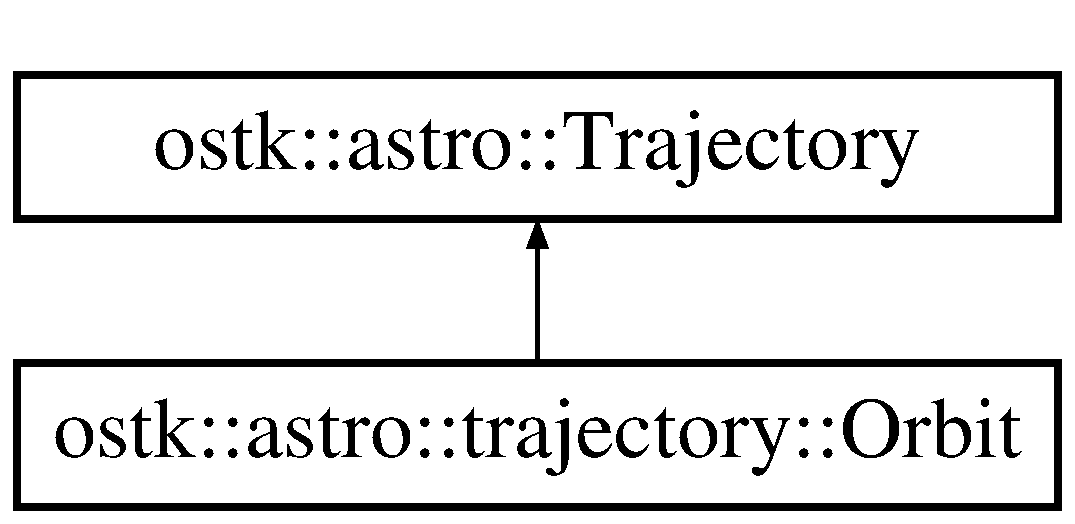
\includegraphics[height=2.000000cm]{classostk_1_1astro_1_1_trajectory}
\end{center}
\end{figure}
\doxysubsection*{Public Member Functions}
\begin{DoxyCompactItemize}
\item 
\mbox{\hyperlink{classostk_1_1astro_1_1_trajectory_a9333200bd6afed5aef4f5aad8a2a8e84}{Trajectory}} (const \mbox{\hyperlink{classostk_1_1astro_1_1trajectory_1_1_model}{Model}} \&a\+Model)
\begin{DoxyCompactList}\small\item\em Constructor (model) \end{DoxyCompactList}\item 
\mbox{\hyperlink{classostk_1_1astro_1_1_trajectory_a5bffa48518940b06d353988efdeb098a}{Trajectory}} (const Array$<$ \mbox{\hyperlink{classostk_1_1astro_1_1trajectory_1_1_state}{State}} $>$ \&a\+State\+Array)
\begin{DoxyCompactList}\small\item\em Constructor (state array) \end{DoxyCompactList}\item 
\mbox{\hyperlink{classostk_1_1astro_1_1_trajectory_a2a7642fa6183da49b5def83f63f08c42}{Trajectory}} (const \mbox{\hyperlink{classostk_1_1astro_1_1_trajectory}{Trajectory}} \&a\+Trajectory)
\begin{DoxyCompactList}\small\item\em Copy constructor. \end{DoxyCompactList}\item 
\mbox{\hyperlink{classostk_1_1astro_1_1_trajectory}{Trajectory}} \& \mbox{\hyperlink{classostk_1_1astro_1_1_trajectory_aa8229045bd7cf0696b8cd235cc3837a8}{operator=}} (const \mbox{\hyperlink{classostk_1_1astro_1_1_trajectory}{Trajectory}} \&a\+Trajectory)
\begin{DoxyCompactList}\small\item\em Copy assignment operator. \end{DoxyCompactList}\item 
bool \mbox{\hyperlink{classostk_1_1astro_1_1_trajectory_a13b1a0621195ed85aa3df0da5ae935f2}{operator==}} (const \mbox{\hyperlink{classostk_1_1astro_1_1_trajectory}{Trajectory}} \&a\+Trajectory) const
\begin{DoxyCompactList}\small\item\em Equal to operator. \end{DoxyCompactList}\item 
bool \mbox{\hyperlink{classostk_1_1astro_1_1_trajectory_abb524dcee260456d546f5e01ee9c228c}{operator!=}} (const \mbox{\hyperlink{classostk_1_1astro_1_1_trajectory}{Trajectory}} \&a\+Trajectory) const
\begin{DoxyCompactList}\small\item\em Not equal to operator. \end{DoxyCompactList}\item 
bool \mbox{\hyperlink{classostk_1_1astro_1_1_trajectory_ab0c02a9844e584b50da35df710b71e81}{is\+Defined}} () const
\begin{DoxyCompactList}\small\item\em Check if trajectory is defined. \end{DoxyCompactList}\item 
const \mbox{\hyperlink{classostk_1_1astro_1_1trajectory_1_1_model}{Model}} \& \mbox{\hyperlink{classostk_1_1astro_1_1_trajectory_a7a5e15ddb0b4e1a1546615840610252c}{access\+Model}} () const
\begin{DoxyCompactList}\small\item\em \mbox{\hyperlink{classostk_1_1astro_1_1_access}{Access}} trajectory model. \end{DoxyCompactList}\item 
\mbox{\hyperlink{classostk_1_1astro_1_1trajectory_1_1_state}{State}} \mbox{\hyperlink{classostk_1_1astro_1_1_trajectory_a0814d622d4bfb55cedb3d8eafd39f640}{get\+State\+At}} (const Instant \&an\+Instant) const
\begin{DoxyCompactList}\small\item\em Get state at a given instant. \end{DoxyCompactList}\item 
Array$<$ \mbox{\hyperlink{classostk_1_1astro_1_1trajectory_1_1_state}{State}} $>$ \mbox{\hyperlink{classostk_1_1astro_1_1_trajectory_a31f02515d567ac57c8d5e06d47da08a8}{get\+States\+At}} (const Array$<$ Instant $>$ \&an\+Instant\+Array) const
\begin{DoxyCompactList}\small\item\em Get states at a given instants. \end{DoxyCompactList}\item 
virtual void \mbox{\hyperlink{classostk_1_1astro_1_1_trajectory_aac11fb7c53f4cf970f52f681a75c5261}{print}} (std\+::ostream \&an\+Output\+Stream, bool display\+Decorator=true) const
\begin{DoxyCompactList}\small\item\em Print trajectory to output stream. \end{DoxyCompactList}\end{DoxyCompactItemize}
\doxysubsection*{Static Public Member Functions}
\begin{DoxyCompactItemize}
\item 
static \mbox{\hyperlink{classostk_1_1astro_1_1_trajectory}{Trajectory}} \mbox{\hyperlink{classostk_1_1astro_1_1_trajectory_a87873d63cae80dff7e43c97dc9b3668f}{Undefined}} ()
\begin{DoxyCompactList}\small\item\em Constructs an undefined trajectory. \end{DoxyCompactList}\item 
static \mbox{\hyperlink{classostk_1_1astro_1_1_trajectory}{Trajectory}} \mbox{\hyperlink{classostk_1_1astro_1_1_trajectory_ae98d1466450030f73a83567c8cc1471a}{Position}} (const physics\+::coord\+::\+Position \&a\+Position)
\begin{DoxyCompactList}\small\item\em Constructs a trajectory from a given position. \end{DoxyCompactList}\end{DoxyCompactItemize}
\doxysubsection*{Friends}
\begin{DoxyCompactItemize}
\item 
std\+::ostream \& \mbox{\hyperlink{classostk_1_1astro_1_1_trajectory_aef0327f0240dc2d71eca34dc287f88ea}{operator$<$$<$}} (std\+::ostream \&an\+Output\+Stream, const \mbox{\hyperlink{classostk_1_1astro_1_1_trajectory}{Trajectory}} \&a\+Trajectory)
\begin{DoxyCompactList}\small\item\em Output stream operator. \end{DoxyCompactList}\end{DoxyCompactItemize}


\doxysubsection{Detailed Description}
Path followed by an object through space as a function of time. 

\href{https://en.wikipedia.org/wiki/Trajectory}{\texttt{ https\+://en.\+wikipedia.\+org/wiki/\+Trajectory}} 

\doxysubsection{Constructor \& Destructor Documentation}
\mbox{\Hypertarget{classostk_1_1astro_1_1_trajectory_a9333200bd6afed5aef4f5aad8a2a8e84}\label{classostk_1_1astro_1_1_trajectory_a9333200bd6afed5aef4f5aad8a2a8e84}} 
\index{ostk::astro::Trajectory@{ostk::astro::Trajectory}!Trajectory@{Trajectory}}
\index{Trajectory@{Trajectory}!ostk::astro::Trajectory@{ostk::astro::Trajectory}}
\doxysubsubsection{\texorpdfstring{Trajectory()}{Trajectory()}\hspace{0.1cm}{\footnotesize\ttfamily [1/3]}}
{\footnotesize\ttfamily ostk\+::astro\+::\+Trajectory\+::\+Trajectory (\begin{DoxyParamCaption}\item[{const \mbox{\hyperlink{classostk_1_1astro_1_1trajectory_1_1_model}{Model}} \&}]{a\+Model }\end{DoxyParamCaption})}



Constructor (model) 


\begin{DoxyCode}{0}
\DoxyCodeLine{Tabulated model = \mbox{\hyperlink{classostk_1_1astro_1_1trajectory_1_1models_1_1_tabulated_a81cf8ebea4354805ab69e732bfe73d77}{Tabulated::Load}}(File::Path(Path::Parse(\textcolor{stringliteral}{"/path/to/trajectory.csv"}))) ;}
\DoxyCodeLine{\mbox{\hyperlink{classostk_1_1astro_1_1_trajectory_a9333200bd6afed5aef4f5aad8a2a8e84}{Trajectory}} trajectory = \{ model \} ;}
\end{DoxyCode}



\begin{DoxyParams}[1]{Parameters}
\mbox{\texttt{ in}}  & {\em a\+Model} & A trajectory model \\
\hline
\end{DoxyParams}
\mbox{\Hypertarget{classostk_1_1astro_1_1_trajectory_a5bffa48518940b06d353988efdeb098a}\label{classostk_1_1astro_1_1_trajectory_a5bffa48518940b06d353988efdeb098a}} 
\index{ostk::astro::Trajectory@{ostk::astro::Trajectory}!Trajectory@{Trajectory}}
\index{Trajectory@{Trajectory}!ostk::astro::Trajectory@{ostk::astro::Trajectory}}
\doxysubsubsection{\texorpdfstring{Trajectory()}{Trajectory()}\hspace{0.1cm}{\footnotesize\ttfamily [2/3]}}
{\footnotesize\ttfamily ostk\+::astro\+::\+Trajectory\+::\+Trajectory (\begin{DoxyParamCaption}\item[{const Array$<$ \mbox{\hyperlink{classostk_1_1astro_1_1trajectory_1_1_state}{State}} $>$ \&}]{a\+State\+Array }\end{DoxyParamCaption})}



Constructor (state array) 


\begin{DoxyCode}{0}
\DoxyCodeLine{Array<State> stateArray = \{ ... \} ;}
\DoxyCodeLine{\mbox{\hyperlink{classostk_1_1astro_1_1_trajectory_a9333200bd6afed5aef4f5aad8a2a8e84}{Trajectory}} trajectory = \{ stateArray \} ;}
\end{DoxyCode}



\begin{DoxyParams}[1]{Parameters}
\mbox{\texttt{ in}}  & {\em a\+State\+Array} & An array of states \\
\hline
\end{DoxyParams}
\mbox{\Hypertarget{classostk_1_1astro_1_1_trajectory_a2a7642fa6183da49b5def83f63f08c42}\label{classostk_1_1astro_1_1_trajectory_a2a7642fa6183da49b5def83f63f08c42}} 
\index{ostk::astro::Trajectory@{ostk::astro::Trajectory}!Trajectory@{Trajectory}}
\index{Trajectory@{Trajectory}!ostk::astro::Trajectory@{ostk::astro::Trajectory}}
\doxysubsubsection{\texorpdfstring{Trajectory()}{Trajectory()}\hspace{0.1cm}{\footnotesize\ttfamily [3/3]}}
{\footnotesize\ttfamily ostk\+::astro\+::\+Trajectory\+::\+Trajectory (\begin{DoxyParamCaption}\item[{const \mbox{\hyperlink{classostk_1_1astro_1_1_trajectory}{Trajectory}} \&}]{a\+Trajectory }\end{DoxyParamCaption})}



Copy constructor. 


\begin{DoxyParams}[1]{Parameters}
\mbox{\texttt{ in}}  & {\em a\+Trajectory} & A trajectory \\
\hline
\end{DoxyParams}


\doxysubsection{Member Function Documentation}
\mbox{\Hypertarget{classostk_1_1astro_1_1_trajectory_a7a5e15ddb0b4e1a1546615840610252c}\label{classostk_1_1astro_1_1_trajectory_a7a5e15ddb0b4e1a1546615840610252c}} 
\index{ostk::astro::Trajectory@{ostk::astro::Trajectory}!accessModel@{accessModel}}
\index{accessModel@{accessModel}!ostk::astro::Trajectory@{ostk::astro::Trajectory}}
\doxysubsubsection{\texorpdfstring{accessModel()}{accessModel()}}
{\footnotesize\ttfamily const \mbox{\hyperlink{classostk_1_1astro_1_1trajectory_1_1_model}{Model}} \& ostk\+::astro\+::\+Trajectory\+::access\+Model (\begin{DoxyParamCaption}{ }\end{DoxyParamCaption}) const}



\mbox{\hyperlink{classostk_1_1astro_1_1_access}{Access}} trajectory model. 

\begin{DoxyReturn}{Returns}
Reference to trajectory model 
\end{DoxyReturn}
\mbox{\Hypertarget{classostk_1_1astro_1_1_trajectory_a0814d622d4bfb55cedb3d8eafd39f640}\label{classostk_1_1astro_1_1_trajectory_a0814d622d4bfb55cedb3d8eafd39f640}} 
\index{ostk::astro::Trajectory@{ostk::astro::Trajectory}!getStateAt@{getStateAt}}
\index{getStateAt@{getStateAt}!ostk::astro::Trajectory@{ostk::astro::Trajectory}}
\doxysubsubsection{\texorpdfstring{getStateAt()}{getStateAt()}}
{\footnotesize\ttfamily \mbox{\hyperlink{classostk_1_1astro_1_1trajectory_1_1_state}{State}} ostk\+::astro\+::\+Trajectory\+::get\+State\+At (\begin{DoxyParamCaption}\item[{const Instant \&}]{an\+Instant }\end{DoxyParamCaption}) const}



Get state at a given instant. 


\begin{DoxyCode}{0}
\DoxyCodeLine{\mbox{\hyperlink{classostk_1_1astro_1_1_trajectory_a9333200bd6afed5aef4f5aad8a2a8e84}{Trajectory}} trajectory = \{ ... \} ;}
\DoxyCodeLine{Instant instant = \{ ... \} ;}
\DoxyCodeLine{State state = trajectory.getStateAt(instant) ;}
\end{DoxyCode}



\begin{DoxyParams}[1]{Parameters}
\mbox{\texttt{ in}}  & {\em an\+Instant} & An instant \\
\hline
\end{DoxyParams}
\begin{DoxyReturn}{Returns}
State 
\end{DoxyReturn}
\mbox{\Hypertarget{classostk_1_1astro_1_1_trajectory_a31f02515d567ac57c8d5e06d47da08a8}\label{classostk_1_1astro_1_1_trajectory_a31f02515d567ac57c8d5e06d47da08a8}} 
\index{ostk::astro::Trajectory@{ostk::astro::Trajectory}!getStatesAt@{getStatesAt}}
\index{getStatesAt@{getStatesAt}!ostk::astro::Trajectory@{ostk::astro::Trajectory}}
\doxysubsubsection{\texorpdfstring{getStatesAt()}{getStatesAt()}}
{\footnotesize\ttfamily Array$<$ \mbox{\hyperlink{classostk_1_1astro_1_1trajectory_1_1_state}{State}} $>$ ostk\+::astro\+::\+Trajectory\+::get\+States\+At (\begin{DoxyParamCaption}\item[{const Array$<$ Instant $>$ \&}]{an\+Instant\+Array }\end{DoxyParamCaption}) const}



Get states at a given instants. 


\begin{DoxyCode}{0}
\DoxyCodeLine{\mbox{\hyperlink{classostk_1_1astro_1_1_trajectory_a9333200bd6afed5aef4f5aad8a2a8e84}{Trajectory}} trajectory = \{ ... \} ;}
\DoxyCodeLine{Array<Instant> instants = \{ ... \} ;}
\DoxyCodeLine{Array<State> state = trajectory.getStatesAt(instants) ;}
\end{DoxyCode}



\begin{DoxyParams}[1]{Parameters}
\mbox{\texttt{ in}}  & {\em an\+Instant\+Array} & An array of instants \\
\hline
\end{DoxyParams}
\begin{DoxyReturn}{Returns}
Array of states 
\end{DoxyReturn}
\mbox{\Hypertarget{classostk_1_1astro_1_1_trajectory_ab0c02a9844e584b50da35df710b71e81}\label{classostk_1_1astro_1_1_trajectory_ab0c02a9844e584b50da35df710b71e81}} 
\index{ostk::astro::Trajectory@{ostk::astro::Trajectory}!isDefined@{isDefined}}
\index{isDefined@{isDefined}!ostk::astro::Trajectory@{ostk::astro::Trajectory}}
\doxysubsubsection{\texorpdfstring{isDefined()}{isDefined()}}
{\footnotesize\ttfamily bool ostk\+::astro\+::\+Trajectory\+::is\+Defined (\begin{DoxyParamCaption}{ }\end{DoxyParamCaption}) const}



Check if trajectory is defined. 


\begin{DoxyCode}{0}
\DoxyCodeLine{\mbox{\hyperlink{classostk_1_1astro_1_1_trajectory_a9333200bd6afed5aef4f5aad8a2a8e84}{Trajectory}}(...).isDefined() ;}
\end{DoxyCode}


\begin{DoxyReturn}{Returns}
True if trajectory is defined 
\end{DoxyReturn}
\mbox{\Hypertarget{classostk_1_1astro_1_1_trajectory_abb524dcee260456d546f5e01ee9c228c}\label{classostk_1_1astro_1_1_trajectory_abb524dcee260456d546f5e01ee9c228c}} 
\index{ostk::astro::Trajectory@{ostk::astro::Trajectory}!operator"!=@{operator"!=}}
\index{operator"!=@{operator"!=}!ostk::astro::Trajectory@{ostk::astro::Trajectory}}
\doxysubsubsection{\texorpdfstring{operator"!=()}{operator!=()}}
{\footnotesize\ttfamily bool ostk\+::astro\+::\+Trajectory\+::operator!= (\begin{DoxyParamCaption}\item[{const \mbox{\hyperlink{classostk_1_1astro_1_1_trajectory}{Trajectory}} \&}]{a\+Trajectory }\end{DoxyParamCaption}) const}



Not equal to operator. 


\begin{DoxyCode}{0}
\DoxyCodeLine{\mbox{\hyperlink{classostk_1_1astro_1_1_trajectory_a9333200bd6afed5aef4f5aad8a2a8e84}{Trajectory}}(...) != \mbox{\hyperlink{classostk_1_1astro_1_1_trajectory_a9333200bd6afed5aef4f5aad8a2a8e84}{Trajectory}}(...) ;}
\end{DoxyCode}



\begin{DoxyParams}[1]{Parameters}
\mbox{\texttt{ in}}  & {\em a\+Trajectory} & A trajectory \\
\hline
\end{DoxyParams}
\begin{DoxyReturn}{Returns}
True if trajectories are not equal 
\end{DoxyReturn}
\mbox{\Hypertarget{classostk_1_1astro_1_1_trajectory_aa8229045bd7cf0696b8cd235cc3837a8}\label{classostk_1_1astro_1_1_trajectory_aa8229045bd7cf0696b8cd235cc3837a8}} 
\index{ostk::astro::Trajectory@{ostk::astro::Trajectory}!operator=@{operator=}}
\index{operator=@{operator=}!ostk::astro::Trajectory@{ostk::astro::Trajectory}}
\doxysubsubsection{\texorpdfstring{operator=()}{operator=()}}
{\footnotesize\ttfamily \mbox{\hyperlink{classostk_1_1astro_1_1_trajectory}{Trajectory}} \& ostk\+::astro\+::\+Trajectory\+::operator= (\begin{DoxyParamCaption}\item[{const \mbox{\hyperlink{classostk_1_1astro_1_1_trajectory}{Trajectory}} \&}]{a\+Trajectory }\end{DoxyParamCaption})}



Copy assignment operator. 

\mbox{\Hypertarget{classostk_1_1astro_1_1_trajectory_a13b1a0621195ed85aa3df0da5ae935f2}\label{classostk_1_1astro_1_1_trajectory_a13b1a0621195ed85aa3df0da5ae935f2}} 
\index{ostk::astro::Trajectory@{ostk::astro::Trajectory}!operator==@{operator==}}
\index{operator==@{operator==}!ostk::astro::Trajectory@{ostk::astro::Trajectory}}
\doxysubsubsection{\texorpdfstring{operator==()}{operator==()}}
{\footnotesize\ttfamily bool ostk\+::astro\+::\+Trajectory\+::operator== (\begin{DoxyParamCaption}\item[{const \mbox{\hyperlink{classostk_1_1astro_1_1_trajectory}{Trajectory}} \&}]{a\+Trajectory }\end{DoxyParamCaption}) const}



Equal to operator. 


\begin{DoxyCode}{0}
\DoxyCodeLine{\mbox{\hyperlink{classostk_1_1astro_1_1_trajectory_a9333200bd6afed5aef4f5aad8a2a8e84}{Trajectory}}(...) == \mbox{\hyperlink{classostk_1_1astro_1_1_trajectory_a9333200bd6afed5aef4f5aad8a2a8e84}{Trajectory}}(...) ;}
\end{DoxyCode}



\begin{DoxyParams}[1]{Parameters}
\mbox{\texttt{ in}}  & {\em a\+Trajectory} & A trajectory \\
\hline
\end{DoxyParams}
\begin{DoxyReturn}{Returns}
True if trajectories are equal 
\end{DoxyReturn}
\mbox{\Hypertarget{classostk_1_1astro_1_1_trajectory_ae98d1466450030f73a83567c8cc1471a}\label{classostk_1_1astro_1_1_trajectory_ae98d1466450030f73a83567c8cc1471a}} 
\index{ostk::astro::Trajectory@{ostk::astro::Trajectory}!Position@{Position}}
\index{Position@{Position}!ostk::astro::Trajectory@{ostk::astro::Trajectory}}
\doxysubsubsection{\texorpdfstring{Position()}{Position()}}
{\footnotesize\ttfamily \mbox{\hyperlink{classostk_1_1astro_1_1_trajectory}{Trajectory}} ostk\+::astro\+::\+Trajectory\+::\+Position (\begin{DoxyParamCaption}\item[{const physics\+::coord\+::\+Position \&}]{a\+Position }\end{DoxyParamCaption})\hspace{0.3cm}{\ttfamily [static]}}



Constructs a trajectory from a given position. 


\begin{DoxyCode}{0}
\DoxyCodeLine{\mbox{\hyperlink{classostk_1_1astro_1_1_trajectory_ae98d1466450030f73a83567c8cc1471a}{Position}} position = Position::Meters(\{ 0.0, 0.0, 0.0 \}, Frame::GCRF()) ;}
\DoxyCodeLine{\mbox{\hyperlink{classostk_1_1astro_1_1_trajectory_a9333200bd6afed5aef4f5aad8a2a8e84}{Trajectory}} trajectory = \mbox{\hyperlink{classostk_1_1astro_1_1_trajectory_ae98d1466450030f73a83567c8cc1471a}{Trajectory::Position}}(position) ;}
\end{DoxyCode}



\begin{DoxyParams}[1]{Parameters}
\mbox{\texttt{ in}}  & {\em a\+Position} & A position \\
\hline
\end{DoxyParams}
\begin{DoxyReturn}{Returns}
Static trajectory 
\end{DoxyReturn}
\mbox{\Hypertarget{classostk_1_1astro_1_1_trajectory_aac11fb7c53f4cf970f52f681a75c5261}\label{classostk_1_1astro_1_1_trajectory_aac11fb7c53f4cf970f52f681a75c5261}} 
\index{ostk::astro::Trajectory@{ostk::astro::Trajectory}!print@{print}}
\index{print@{print}!ostk::astro::Trajectory@{ostk::astro::Trajectory}}
\doxysubsubsection{\texorpdfstring{print()}{print()}}
{\footnotesize\ttfamily void ostk\+::astro\+::\+Trajectory\+::print (\begin{DoxyParamCaption}\item[{std\+::ostream \&}]{an\+Output\+Stream,  }\item[{bool}]{display\+Decorator = {\ttfamily true} }\end{DoxyParamCaption}) const\hspace{0.3cm}{\ttfamily [virtual]}}



Print trajectory to output stream. 


\begin{DoxyCode}{0}
\DoxyCodeLine{\mbox{\hyperlink{classostk_1_1astro_1_1_trajectory_a9333200bd6afed5aef4f5aad8a2a8e84}{Trajectory}} trajectory = \{ ... \} ;}
\DoxyCodeLine{trajectory.print(std::cout, \textcolor{keyword}{true}) ;}
\end{DoxyCode}



\begin{DoxyParams}[1]{Parameters}
\mbox{\texttt{ in}}  & {\em an\+Output\+Stream} & An output stream \\
\hline
\mbox{\texttt{ in}}  & {\em display\+Decorator} & If true, display decorator \\
\hline
\end{DoxyParams}


Reimplemented in \mbox{\hyperlink{classostk_1_1astro_1_1trajectory_1_1_orbit_ae890e832785f84c3f03c1e103f952826}{ostk\+::astro\+::trajectory\+::\+Orbit}}.

\mbox{\Hypertarget{classostk_1_1astro_1_1_trajectory_a87873d63cae80dff7e43c97dc9b3668f}\label{classostk_1_1astro_1_1_trajectory_a87873d63cae80dff7e43c97dc9b3668f}} 
\index{ostk::astro::Trajectory@{ostk::astro::Trajectory}!Undefined@{Undefined}}
\index{Undefined@{Undefined}!ostk::astro::Trajectory@{ostk::astro::Trajectory}}
\doxysubsubsection{\texorpdfstring{Undefined()}{Undefined()}}
{\footnotesize\ttfamily \mbox{\hyperlink{classostk_1_1astro_1_1_trajectory}{Trajectory}} ostk\+::astro\+::\+Trajectory\+::\+Undefined (\begin{DoxyParamCaption}{ }\end{DoxyParamCaption})\hspace{0.3cm}{\ttfamily [static]}}



Constructs an undefined trajectory. 


\begin{DoxyCode}{0}
\DoxyCodeLine{\mbox{\hyperlink{classostk_1_1astro_1_1_trajectory_a9333200bd6afed5aef4f5aad8a2a8e84}{Trajectory}} trajectory = \mbox{\hyperlink{classostk_1_1astro_1_1_trajectory_a87873d63cae80dff7e43c97dc9b3668f}{Trajectory::Undefined}}() ; \textcolor{comment}{// Undefined}}
\end{DoxyCode}


\begin{DoxyReturn}{Returns}
Undefined trajectory 
\end{DoxyReturn}


\doxysubsection{Friends And Related Function Documentation}
\mbox{\Hypertarget{classostk_1_1astro_1_1_trajectory_aef0327f0240dc2d71eca34dc287f88ea}\label{classostk_1_1astro_1_1_trajectory_aef0327f0240dc2d71eca34dc287f88ea}} 
\index{ostk::astro::Trajectory@{ostk::astro::Trajectory}!operator$<$$<$@{operator$<$$<$}}
\index{operator$<$$<$@{operator$<$$<$}!ostk::astro::Trajectory@{ostk::astro::Trajectory}}
\doxysubsubsection{\texorpdfstring{operator$<$$<$}{operator<<}}
{\footnotesize\ttfamily std\+::ostream\& operator$<$$<$ (\begin{DoxyParamCaption}\item[{std\+::ostream \&}]{an\+Output\+Stream,  }\item[{const \mbox{\hyperlink{classostk_1_1astro_1_1_trajectory}{Trajectory}} \&}]{a\+Trajectory }\end{DoxyParamCaption})\hspace{0.3cm}{\ttfamily [friend]}}



Output stream operator. 


\begin{DoxyCode}{0}
\DoxyCodeLine{std::cout << \mbox{\hyperlink{classostk_1_1astro_1_1_trajectory_a9333200bd6afed5aef4f5aad8a2a8e84}{Trajectory}}(...) ;}
\end{DoxyCode}



\begin{DoxyParams}[1]{Parameters}
\mbox{\texttt{ in}}  & {\em an\+Output\+Stream} & An output stream \\
\hline
\mbox{\texttt{ in}}  & {\em a\+Trajectory} & A trajectory \\
\hline
\end{DoxyParams}
\begin{DoxyReturn}{Returns}
A reference to output stream 
\end{DoxyReturn}


The documentation for this class was generated from the following files\+:\begin{DoxyCompactItemize}
\item 
include/\+Open\+Space\+Toolkit/\+Astrodynamics/\mbox{\hyperlink{_trajectory_8hpp}{Trajectory.\+hpp}}\item 
src/\+Open\+Space\+Toolkit/\+Astrodynamics/\mbox{\hyperlink{_trajectory_8cpp}{Trajectory.\+cpp}}\end{DoxyCompactItemize}

\hypertarget{classostk_1_1astro_1_1flight_1_1profile_1_1models_1_1_transform}{}\doxysection{ostk\+::astro\+::flight\+::profile\+::models\+::Transform Class Reference}
\label{classostk_1_1astro_1_1flight_1_1profile_1_1models_1_1_transform}\index{ostk::astro::flight::profile::models::Transform@{ostk::astro::flight::profile::models::Transform}}


\mbox{\hyperlink{classostk_1_1astro_1_1flight_1_1profile_1_1models_1_1_transform}{Transform}} provided profile model.  




{\ttfamily \#include $<$Transform.\+hpp$>$}

Inheritance diagram for ostk\+::astro\+::flight\+::profile\+::models\+::Transform\+:\begin{figure}[H]
\begin{center}
\leavevmode
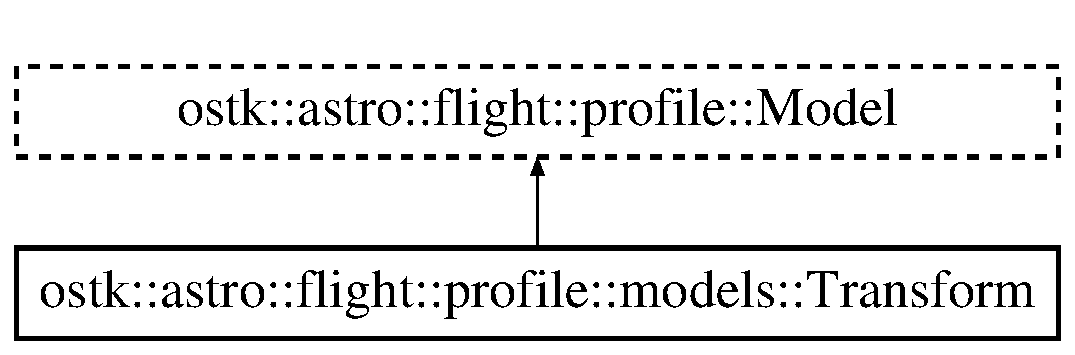
\includegraphics[height=2.000000cm]{classostk_1_1astro_1_1flight_1_1profile_1_1models_1_1_transform}
\end{center}
\end{figure}
\doxysubsection*{Public Member Functions}
\begin{DoxyCompactItemize}
\item 
\mbox{\hyperlink{classostk_1_1astro_1_1flight_1_1profile_1_1models_1_1_transform_a95d76db47af0764c1a05c32298799d72}{Transform}} (const \mbox{\hyperlink{namespaceostk_1_1astro_1_1flight_1_1profile_1_1models_a7e9732cb31adb5d5c1f85f7bad1f3424}{Dynamic\+Provider}} \&a\+Dynamic\+Transform\+Provider, const Shared$<$ const Frame $>$ \&a\+Frame\+S\+Ptr)
\item 
virtual \mbox{\hyperlink{classostk_1_1astro_1_1flight_1_1profile_1_1models_1_1_transform}{Transform}} $\ast$ \mbox{\hyperlink{classostk_1_1astro_1_1flight_1_1profile_1_1models_1_1_transform_aafd4791dacf320ddedddefbc8d0f2e0e}{clone}} () const override
\item 
virtual bool \mbox{\hyperlink{classostk_1_1astro_1_1flight_1_1profile_1_1models_1_1_transform_a2d0f1f3cc3f340c5617125bea08a9930}{is\+Defined}} () const override
\item 
virtual \mbox{\hyperlink{classostk_1_1astro_1_1flight_1_1profile_1_1_state}{State}} \mbox{\hyperlink{classostk_1_1astro_1_1flight_1_1profile_1_1models_1_1_transform_a6288febae942c92508173db08b4554b0}{calculate\+State\+At}} (const Instant \&an\+Instant) const override
\item 
virtual Axes \mbox{\hyperlink{classostk_1_1astro_1_1flight_1_1profile_1_1models_1_1_transform_a7eb8b58fd5f72e8ee9aa3b94cd0ffaaa}{get\+Axes\+At}} (const Instant \&an\+Instant) const override
\item 
virtual Shared$<$ const Frame $>$ \mbox{\hyperlink{classostk_1_1astro_1_1flight_1_1profile_1_1models_1_1_transform_a7fa6ee57c59b5bff2c60001c11cac04c}{get\+Body\+Frame}} (const String \&a\+Frame\+Name) const override
\item 
virtual void \mbox{\hyperlink{classostk_1_1astro_1_1flight_1_1profile_1_1models_1_1_transform_aef9a20156493d68570a989d87ac2f9f6}{print}} (std\+::ostream \&an\+Output\+Stream, bool display\+Decorator=true) const override
\end{DoxyCompactItemize}
\doxysubsection*{Static Public Member Functions}
\begin{DoxyCompactItemize}
\item 
static \mbox{\hyperlink{classostk_1_1astro_1_1flight_1_1profile_1_1models_1_1_transform}{Transform}} \mbox{\hyperlink{classostk_1_1astro_1_1flight_1_1profile_1_1models_1_1_transform_a06ac043e7d6577f51578fc14331e1c6d}{Undefined}} ()
\item 
static \mbox{\hyperlink{classostk_1_1astro_1_1flight_1_1profile_1_1models_1_1_transform}{Transform}} \mbox{\hyperlink{classostk_1_1astro_1_1flight_1_1profile_1_1models_1_1_transform_ad09043542f34243cfa200d74db5c47bf}{Inertial\+Pointing}} (const \mbox{\hyperlink{classostk_1_1astro_1_1_trajectory}{Trajectory}} \&a\+Trajectory, const Quaternion \&a\+Quaternion)
\begin{DoxyCompactList}\small\item\em Constructs a flight profile with inertial pointing. \end{DoxyCompactList}\item 
static \mbox{\hyperlink{classostk_1_1astro_1_1flight_1_1profile_1_1models_1_1_transform}{Transform}} \mbox{\hyperlink{classostk_1_1astro_1_1flight_1_1profile_1_1models_1_1_transform_a45cbb8066c7a6c56774746c3ea025c8d}{Nadir\+Pointing}} (const \mbox{\hyperlink{classostk_1_1astro_1_1trajectory_1_1_orbit}{trajectory\+::\+Orbit}} \&an\+Orbit, const \mbox{\hyperlink{classostk_1_1astro_1_1trajectory_1_1_orbit_a1cc449ad56374471a8ab4300dde979e7}{trajectory\+::\+Orbit\+::\+Frame\+Type}} \&an\+Orbital\+Frame\+Type)
\begin{DoxyCompactList}\small\item\em Constructs a flight profile with nadir pointing. \end{DoxyCompactList}\end{DoxyCompactItemize}
\doxysubsection*{Protected Member Functions}
\begin{DoxyCompactItemize}
\item 
virtual bool \mbox{\hyperlink{classostk_1_1astro_1_1flight_1_1profile_1_1models_1_1_transform_ad49694ca5cfb4fabf17ac063d9953fb0}{operator==}} (const \mbox{\hyperlink{classostk_1_1astro_1_1flight_1_1profile_1_1_model}{Model}} \&a\+Model) const override
\end{DoxyCompactItemize}
\doxysubsection*{Friends}
\begin{DoxyCompactItemize}
\item 
std\+::ostream \& \mbox{\hyperlink{classostk_1_1astro_1_1flight_1_1profile_1_1models_1_1_transform_a31ed56d1b0b19d8f7363743664717403}{operator$<$$<$}} (std\+::ostream \&an\+Output\+Stream, const \mbox{\hyperlink{classostk_1_1astro_1_1flight_1_1profile_1_1models_1_1_transform}{Transform}} \&a\+Transform\+Model)
\end{DoxyCompactItemize}


\doxysubsection{Detailed Description}
\mbox{\hyperlink{classostk_1_1astro_1_1flight_1_1profile_1_1models_1_1_transform}{Transform}} provided profile model. 

\doxysubsection{Constructor \& Destructor Documentation}
\mbox{\Hypertarget{classostk_1_1astro_1_1flight_1_1profile_1_1models_1_1_transform_a95d76db47af0764c1a05c32298799d72}\label{classostk_1_1astro_1_1flight_1_1profile_1_1models_1_1_transform_a95d76db47af0764c1a05c32298799d72}} 
\index{ostk::astro::flight::profile::models::Transform@{ostk::astro::flight::profile::models::Transform}!Transform@{Transform}}
\index{Transform@{Transform}!ostk::astro::flight::profile::models::Transform@{ostk::astro::flight::profile::models::Transform}}
\doxysubsubsection{\texorpdfstring{Transform()}{Transform()}}
{\footnotesize\ttfamily ostk\+::astro\+::flight\+::profile\+::models\+::\+Transform\+::\+Transform (\begin{DoxyParamCaption}\item[{const \mbox{\hyperlink{namespaceostk_1_1astro_1_1flight_1_1profile_1_1models_a7e9732cb31adb5d5c1f85f7bad1f3424}{Dynamic\+Provider}} \&}]{a\+Dynamic\+Transform\+Provider,  }\item[{const Shared$<$ const Frame $>$ \&}]{a\+Frame\+S\+Ptr }\end{DoxyParamCaption})}



\doxysubsection{Member Function Documentation}
\mbox{\Hypertarget{classostk_1_1astro_1_1flight_1_1profile_1_1models_1_1_transform_a6288febae942c92508173db08b4554b0}\label{classostk_1_1astro_1_1flight_1_1profile_1_1models_1_1_transform_a6288febae942c92508173db08b4554b0}} 
\index{ostk::astro::flight::profile::models::Transform@{ostk::astro::flight::profile::models::Transform}!calculateStateAt@{calculateStateAt}}
\index{calculateStateAt@{calculateStateAt}!ostk::astro::flight::profile::models::Transform@{ostk::astro::flight::profile::models::Transform}}
\doxysubsubsection{\texorpdfstring{calculateStateAt()}{calculateStateAt()}}
{\footnotesize\ttfamily \mbox{\hyperlink{classostk_1_1astro_1_1flight_1_1profile_1_1_state}{State}} ostk\+::astro\+::flight\+::profile\+::models\+::\+Transform\+::calculate\+State\+At (\begin{DoxyParamCaption}\item[{const Instant \&}]{an\+Instant }\end{DoxyParamCaption}) const\hspace{0.3cm}{\ttfamily [override]}, {\ttfamily [virtual]}}



Implements \mbox{\hyperlink{classostk_1_1astro_1_1flight_1_1profile_1_1_model_a1b205fa29b50fcfc06c99234a8579eb8}{ostk\+::astro\+::flight\+::profile\+::\+Model}}.

\mbox{\Hypertarget{classostk_1_1astro_1_1flight_1_1profile_1_1models_1_1_transform_aafd4791dacf320ddedddefbc8d0f2e0e}\label{classostk_1_1astro_1_1flight_1_1profile_1_1models_1_1_transform_aafd4791dacf320ddedddefbc8d0f2e0e}} 
\index{ostk::astro::flight::profile::models::Transform@{ostk::astro::flight::profile::models::Transform}!clone@{clone}}
\index{clone@{clone}!ostk::astro::flight::profile::models::Transform@{ostk::astro::flight::profile::models::Transform}}
\doxysubsubsection{\texorpdfstring{clone()}{clone()}}
{\footnotesize\ttfamily \mbox{\hyperlink{classostk_1_1astro_1_1flight_1_1profile_1_1models_1_1_transform}{Transform}} $\ast$ ostk\+::astro\+::flight\+::profile\+::models\+::\+Transform\+::clone (\begin{DoxyParamCaption}{ }\end{DoxyParamCaption}) const\hspace{0.3cm}{\ttfamily [override]}, {\ttfamily [virtual]}}



Implements \mbox{\hyperlink{classostk_1_1astro_1_1flight_1_1profile_1_1_model_aabf68c114849fa16a570b694579da40f}{ostk\+::astro\+::flight\+::profile\+::\+Model}}.

\mbox{\Hypertarget{classostk_1_1astro_1_1flight_1_1profile_1_1models_1_1_transform_a7eb8b58fd5f72e8ee9aa3b94cd0ffaaa}\label{classostk_1_1astro_1_1flight_1_1profile_1_1models_1_1_transform_a7eb8b58fd5f72e8ee9aa3b94cd0ffaaa}} 
\index{ostk::astro::flight::profile::models::Transform@{ostk::astro::flight::profile::models::Transform}!getAxesAt@{getAxesAt}}
\index{getAxesAt@{getAxesAt}!ostk::astro::flight::profile::models::Transform@{ostk::astro::flight::profile::models::Transform}}
\doxysubsubsection{\texorpdfstring{getAxesAt()}{getAxesAt()}}
{\footnotesize\ttfamily Axes ostk\+::astro\+::flight\+::profile\+::models\+::\+Transform\+::get\+Axes\+At (\begin{DoxyParamCaption}\item[{const Instant \&}]{an\+Instant }\end{DoxyParamCaption}) const\hspace{0.3cm}{\ttfamily [override]}, {\ttfamily [virtual]}}



Implements \mbox{\hyperlink{classostk_1_1astro_1_1flight_1_1profile_1_1_model_ab18bd79e421c36df4ab716649ce549cd}{ostk\+::astro\+::flight\+::profile\+::\+Model}}.

\mbox{\Hypertarget{classostk_1_1astro_1_1flight_1_1profile_1_1models_1_1_transform_a7fa6ee57c59b5bff2c60001c11cac04c}\label{classostk_1_1astro_1_1flight_1_1profile_1_1models_1_1_transform_a7fa6ee57c59b5bff2c60001c11cac04c}} 
\index{ostk::astro::flight::profile::models::Transform@{ostk::astro::flight::profile::models::Transform}!getBodyFrame@{getBodyFrame}}
\index{getBodyFrame@{getBodyFrame}!ostk::astro::flight::profile::models::Transform@{ostk::astro::flight::profile::models::Transform}}
\doxysubsubsection{\texorpdfstring{getBodyFrame()}{getBodyFrame()}}
{\footnotesize\ttfamily Shared$<$ const Frame $>$ ostk\+::astro\+::flight\+::profile\+::models\+::\+Transform\+::get\+Body\+Frame (\begin{DoxyParamCaption}\item[{const String \&}]{a\+Frame\+Name }\end{DoxyParamCaption}) const\hspace{0.3cm}{\ttfamily [override]}, {\ttfamily [virtual]}}



Implements \mbox{\hyperlink{classostk_1_1astro_1_1flight_1_1profile_1_1_model_a04ded49c09d9a44820251c48f47d0ffa}{ostk\+::astro\+::flight\+::profile\+::\+Model}}.

\mbox{\Hypertarget{classostk_1_1astro_1_1flight_1_1profile_1_1models_1_1_transform_ad09043542f34243cfa200d74db5c47bf}\label{classostk_1_1astro_1_1flight_1_1profile_1_1models_1_1_transform_ad09043542f34243cfa200d74db5c47bf}} 
\index{ostk::astro::flight::profile::models::Transform@{ostk::astro::flight::profile::models::Transform}!InertialPointing@{InertialPointing}}
\index{InertialPointing@{InertialPointing}!ostk::astro::flight::profile::models::Transform@{ostk::astro::flight::profile::models::Transform}}
\doxysubsubsection{\texorpdfstring{InertialPointing()}{InertialPointing()}}
{\footnotesize\ttfamily \mbox{\hyperlink{classostk_1_1astro_1_1flight_1_1profile_1_1models_1_1_transform}{Transform}} ostk\+::astro\+::flight\+::profile\+::models\+::\+Transform\+::\+Inertial\+Pointing (\begin{DoxyParamCaption}\item[{const \mbox{\hyperlink{classostk_1_1astro_1_1_trajectory}{Trajectory}} \&}]{a\+Trajectory,  }\item[{const Quaternion \&}]{a\+Quaternion }\end{DoxyParamCaption})\hspace{0.3cm}{\ttfamily [static]}}



Constructs a flight profile with inertial pointing. 


\begin{DoxyParams}{Parameters}
{\em a\+Trajectory} & A trajectory \\
\hline
{\em a\+Quaternion} & A pointing in G\+C\+RF \\
\hline
\end{DoxyParams}
\begin{DoxyReturn}{Returns}
Flight profile 
\end{DoxyReturn}
\mbox{\Hypertarget{classostk_1_1astro_1_1flight_1_1profile_1_1models_1_1_transform_a2d0f1f3cc3f340c5617125bea08a9930}\label{classostk_1_1astro_1_1flight_1_1profile_1_1models_1_1_transform_a2d0f1f3cc3f340c5617125bea08a9930}} 
\index{ostk::astro::flight::profile::models::Transform@{ostk::astro::flight::profile::models::Transform}!isDefined@{isDefined}}
\index{isDefined@{isDefined}!ostk::astro::flight::profile::models::Transform@{ostk::astro::flight::profile::models::Transform}}
\doxysubsubsection{\texorpdfstring{isDefined()}{isDefined()}}
{\footnotesize\ttfamily bool ostk\+::astro\+::flight\+::profile\+::models\+::\+Transform\+::is\+Defined (\begin{DoxyParamCaption}{ }\end{DoxyParamCaption}) const\hspace{0.3cm}{\ttfamily [override]}, {\ttfamily [virtual]}}



Implements \mbox{\hyperlink{classostk_1_1astro_1_1flight_1_1profile_1_1_model_a0af64ad25ed8d8b2510a70bfe5bcb971}{ostk\+::astro\+::flight\+::profile\+::\+Model}}.

\mbox{\Hypertarget{classostk_1_1astro_1_1flight_1_1profile_1_1models_1_1_transform_a45cbb8066c7a6c56774746c3ea025c8d}\label{classostk_1_1astro_1_1flight_1_1profile_1_1models_1_1_transform_a45cbb8066c7a6c56774746c3ea025c8d}} 
\index{ostk::astro::flight::profile::models::Transform@{ostk::astro::flight::profile::models::Transform}!NadirPointing@{NadirPointing}}
\index{NadirPointing@{NadirPointing}!ostk::astro::flight::profile::models::Transform@{ostk::astro::flight::profile::models::Transform}}
\doxysubsubsection{\texorpdfstring{NadirPointing()}{NadirPointing()}}
{\footnotesize\ttfamily \mbox{\hyperlink{classostk_1_1astro_1_1flight_1_1profile_1_1models_1_1_transform}{Transform}} ostk\+::astro\+::flight\+::profile\+::models\+::\+Transform\+::\+Nadir\+Pointing (\begin{DoxyParamCaption}\item[{const \mbox{\hyperlink{classostk_1_1astro_1_1trajectory_1_1_orbit}{trajectory\+::\+Orbit}} \&}]{an\+Orbit,  }\item[{const \mbox{\hyperlink{classostk_1_1astro_1_1trajectory_1_1_orbit_a1cc449ad56374471a8ab4300dde979e7}{trajectory\+::\+Orbit\+::\+Frame\+Type}} \&}]{an\+Orbital\+Frame\+Type }\end{DoxyParamCaption})\hspace{0.3cm}{\ttfamily [static]}}



Constructs a flight profile with nadir pointing. 


\begin{DoxyParams}{Parameters}
{\em an\+Orbit} & An orbit \\
\hline
{\em an\+Orbital\+Frame\+Type} & An orbital frame type \\
\hline
\end{DoxyParams}
\begin{DoxyReturn}{Returns}
Flight profile 
\end{DoxyReturn}
\mbox{\Hypertarget{classostk_1_1astro_1_1flight_1_1profile_1_1models_1_1_transform_ad49694ca5cfb4fabf17ac063d9953fb0}\label{classostk_1_1astro_1_1flight_1_1profile_1_1models_1_1_transform_ad49694ca5cfb4fabf17ac063d9953fb0}} 
\index{ostk::astro::flight::profile::models::Transform@{ostk::astro::flight::profile::models::Transform}!operator==@{operator==}}
\index{operator==@{operator==}!ostk::astro::flight::profile::models::Transform@{ostk::astro::flight::profile::models::Transform}}
\doxysubsubsection{\texorpdfstring{operator==()}{operator==()}}
{\footnotesize\ttfamily bool ostk\+::astro\+::flight\+::profile\+::models\+::\+Transform\+::operator== (\begin{DoxyParamCaption}\item[{const \mbox{\hyperlink{classostk_1_1astro_1_1flight_1_1profile_1_1_model}{Model}} \&}]{a\+Model }\end{DoxyParamCaption}) const\hspace{0.3cm}{\ttfamily [override]}, {\ttfamily [protected]}, {\ttfamily [virtual]}}



Implements \mbox{\hyperlink{classostk_1_1astro_1_1flight_1_1profile_1_1_model_a87f7ca747d79619e4b4bc04aa6a9252a}{ostk\+::astro\+::flight\+::profile\+::\+Model}}.

\mbox{\Hypertarget{classostk_1_1astro_1_1flight_1_1profile_1_1models_1_1_transform_aef9a20156493d68570a989d87ac2f9f6}\label{classostk_1_1astro_1_1flight_1_1profile_1_1models_1_1_transform_aef9a20156493d68570a989d87ac2f9f6}} 
\index{ostk::astro::flight::profile::models::Transform@{ostk::astro::flight::profile::models::Transform}!print@{print}}
\index{print@{print}!ostk::astro::flight::profile::models::Transform@{ostk::astro::flight::profile::models::Transform}}
\doxysubsubsection{\texorpdfstring{print()}{print()}}
{\footnotesize\ttfamily void ostk\+::astro\+::flight\+::profile\+::models\+::\+Transform\+::print (\begin{DoxyParamCaption}\item[{std\+::ostream \&}]{an\+Output\+Stream,  }\item[{bool}]{display\+Decorator = {\ttfamily true} }\end{DoxyParamCaption}) const\hspace{0.3cm}{\ttfamily [override]}, {\ttfamily [virtual]}}



Implements \mbox{\hyperlink{classostk_1_1astro_1_1flight_1_1profile_1_1_model_ad9bb86b1869150e2bd970e9fa59ce36e}{ostk\+::astro\+::flight\+::profile\+::\+Model}}.

\mbox{\Hypertarget{classostk_1_1astro_1_1flight_1_1profile_1_1models_1_1_transform_a06ac043e7d6577f51578fc14331e1c6d}\label{classostk_1_1astro_1_1flight_1_1profile_1_1models_1_1_transform_a06ac043e7d6577f51578fc14331e1c6d}} 
\index{ostk::astro::flight::profile::models::Transform@{ostk::astro::flight::profile::models::Transform}!Undefined@{Undefined}}
\index{Undefined@{Undefined}!ostk::astro::flight::profile::models::Transform@{ostk::astro::flight::profile::models::Transform}}
\doxysubsubsection{\texorpdfstring{Undefined()}{Undefined()}}
{\footnotesize\ttfamily \mbox{\hyperlink{classostk_1_1astro_1_1flight_1_1profile_1_1models_1_1_transform}{Transform}} ostk\+::astro\+::flight\+::profile\+::models\+::\+Transform\+::\+Undefined (\begin{DoxyParamCaption}{ }\end{DoxyParamCaption})\hspace{0.3cm}{\ttfamily [static]}}



\doxysubsection{Friends And Related Function Documentation}
\mbox{\Hypertarget{classostk_1_1astro_1_1flight_1_1profile_1_1models_1_1_transform_a31ed56d1b0b19d8f7363743664717403}\label{classostk_1_1astro_1_1flight_1_1profile_1_1models_1_1_transform_a31ed56d1b0b19d8f7363743664717403}} 
\index{ostk::astro::flight::profile::models::Transform@{ostk::astro::flight::profile::models::Transform}!operator$<$$<$@{operator$<$$<$}}
\index{operator$<$$<$@{operator$<$$<$}!ostk::astro::flight::profile::models::Transform@{ostk::astro::flight::profile::models::Transform}}
\doxysubsubsection{\texorpdfstring{operator$<$$<$}{operator<<}}
{\footnotesize\ttfamily std\+::ostream\& operator$<$$<$ (\begin{DoxyParamCaption}\item[{std\+::ostream \&}]{an\+Output\+Stream,  }\item[{const \mbox{\hyperlink{classostk_1_1astro_1_1flight_1_1profile_1_1models_1_1_transform}{Transform}} \&}]{a\+Transform\+Model }\end{DoxyParamCaption})\hspace{0.3cm}{\ttfamily [friend]}}



The documentation for this class was generated from the following files\+:\begin{DoxyCompactItemize}
\item 
include/\+Open\+Space\+Toolkit/\+Astrodynamics/\+Flight/\+Profile/\+Models/\mbox{\hyperlink{_transform_8hpp}{Transform.\+hpp}}\item 
src/\+Open\+Space\+Toolkit/\+Astrodynamics/\+Flight/\+Profile/\+Models/\mbox{\hyperlink{_transform_8cpp}{Transform.\+cpp}}\end{DoxyCompactItemize}

\chapter{File Documentation}
\hypertarget{_c_o_n_t_r_i_b_u_t_i_n_g_8md}{}\doxysection{C\+O\+N\+T\+R\+I\+B\+U\+T\+I\+N\+G.\+md File Reference}
\label{_c_o_n_t_r_i_b_u_t_i_n_g_8md}\index{CONTRIBUTING.md@{CONTRIBUTING.md}}

\hypertarget{_tutorial_8md}{}\doxysection{docs/\+Tutorial.md File Reference}
\label{_tutorial_8md}\index{docs/Tutorial.md@{docs/Tutorial.md}}

\hypertarget{_access_8hpp}{}\doxysection{include/\+Open\+Space\+Toolkit/\+Astrodynamics/\+Access.hpp File Reference}
\label{_access_8hpp}\index{include/OpenSpaceToolkit/Astrodynamics/Access.hpp@{include/OpenSpaceToolkit/Astrodynamics/Access.hpp}}
{\ttfamily \#include $<$Open\+Space\+Toolkit/\+Physics/\+Time/\+Interval.\+hpp$>$}\newline
{\ttfamily \#include $<$Open\+Space\+Toolkit/\+Physics/\+Time/\+Duration.\+hpp$>$}\newline
{\ttfamily \#include $<$Open\+Space\+Toolkit/\+Physics/\+Time/\+Instant.\+hpp$>$}\newline
{\ttfamily \#include $<$Open\+Space\+Toolkit/\+Physics/\+Units/\+Derived/\+Angle.\+hpp$>$}\newline
{\ttfamily \#include $<$Open\+Space\+Toolkit/\+Core/\+Containers/\+Array.\+hpp$>$}\newline
{\ttfamily \#include $<$Open\+Space\+Toolkit/\+Core/\+Types/\+String.\+hpp$>$}\newline
\doxysubsection*{Classes}
\begin{DoxyCompactItemize}
\item 
class \mbox{\hyperlink{classostk_1_1astro_1_1_access}{ostk\+::astro\+::\+Access}}
\begin{DoxyCompactList}\small\item\em Object-\/to-\/object visibility. \end{DoxyCompactList}\end{DoxyCompactItemize}
\doxysubsection*{Namespaces}
\begin{DoxyCompactItemize}
\item 
 \mbox{\hyperlink{namespaceostk}{ostk}}
\item 
 \mbox{\hyperlink{namespaceostk_1_1astro}{ostk\+::astro}}
\end{DoxyCompactItemize}


\doxysubsection{Detailed Description}
@project Open Space Toolkit ▸ Astrodynamics

\begin{DoxyAuthor}{Author}
Lucas Brémond \href{mailto:lucas@loftorbital.com}{\texttt{ lucas@loftorbital.\+com}} @license Apache License 2.\+0 
\end{DoxyAuthor}

\hypertarget{_generator_8hpp}{}\doxysection{include/\+Open\+Space\+Toolkit/\+Astrodynamics/\+Access/\+Generator.hpp File Reference}
\label{_generator_8hpp}\index{include/OpenSpaceToolkit/Astrodynamics/Access/Generator.hpp@{include/OpenSpaceToolkit/Astrodynamics/Access/Generator.hpp}}
{\ttfamily \#include $<$Open\+Space\+Toolkit/\+Core/\+Containers/\+Array.\+hpp$>$}\newline
{\ttfamily \#include $<$Open\+Space\+Toolkit/\+Core/\+Containers/\+Map.\+hpp$>$}\newline
{\ttfamily \#include $<$Open\+Space\+Toolkit/\+Core/\+Types/\+Real.\+hpp$>$}\newline
{\ttfamily \#include $<$Open\+Space\+Toolkit/\+Mathematics/\+Objects/\+Interval.\+hpp$>$}\newline
{\ttfamily \#include $<$Open\+Space\+Toolkit/\+Physics/\+Coordinate/\+Spherical/\+A\+E\+R.\+hpp$>$}\newline
{\ttfamily \#include $<$Open\+Space\+Toolkit/\+Physics/\+Environment.\+hpp$>$}\newline
{\ttfamily \#include $<$Open\+Space\+Toolkit/\+Physics/\+Time/\+Instant.\+hpp$>$}\newline
{\ttfamily \#include $<$Open\+Space\+Toolkit/\+Physics/\+Time/\+Interval.\+hpp$>$}\newline
{\ttfamily \#include $<$Open\+Space\+Toolkit/\+Physics/\+Units/\+Derived/\+Angle.\+hpp$>$}\newline
{\ttfamily \#include $<$Open\+Space\+Toolkit/\+Physics/\+Units/\+Length.\+hpp$>$}\newline
{\ttfamily \#include $<$Open\+Space\+Toolkit/\+Astrodynamics/\+Access.\+hpp$>$}\newline
{\ttfamily \#include $<$Open\+Space\+Toolkit/\+Astrodynamics/\+Trajectory.\+hpp$>$}\newline
\doxysubsection*{Classes}
\begin{DoxyCompactItemize}
\item 
class \mbox{\hyperlink{classostk_1_1astro_1_1access_1_1_generator}{ostk\+::astro\+::access\+::\+Generator}}
\end{DoxyCompactItemize}
\doxysubsection*{Namespaces}
\begin{DoxyCompactItemize}
\item 
 \mbox{\hyperlink{namespaceostk}{ostk}}
\begin{DoxyCompactList}\small\item\em Apache License 2.\+0. \end{DoxyCompactList}\item 
 \mbox{\hyperlink{namespaceostk_1_1astro}{ostk\+::astro}}
\item 
 \mbox{\hyperlink{namespaceostk_1_1astro_1_1access}{ostk\+::astro\+::access}}
\end{DoxyCompactItemize}
\doxysubsection*{Macros}
\begin{DoxyCompactItemize}
\item 
\#define \mbox{\hyperlink{_generator_8hpp_a7ce1d4cc8c33e65c078f721b17b975ea}{D\+E\+F\+A\+U\+L\+T\+\_\+\+S\+T\+EP}}~Duration\+::\+Minutes(1.\+0)
\item 
\#define \mbox{\hyperlink{_generator_8hpp_a0e355e0dcb761f1b89524e0e77fd14bd}{D\+E\+F\+A\+U\+L\+T\+\_\+\+T\+O\+L\+E\+R\+A\+N\+CE}}~Duration\+::\+Microseconds(1.\+0)
\end{DoxyCompactItemize}


\doxysubsection{Macro Definition Documentation}
\mbox{\Hypertarget{_generator_8hpp_a7ce1d4cc8c33e65c078f721b17b975ea}\label{_generator_8hpp_a7ce1d4cc8c33e65c078f721b17b975ea}} 
\index{Generator.hpp@{Generator.hpp}!DEFAULT\_STEP@{DEFAULT\_STEP}}
\index{DEFAULT\_STEP@{DEFAULT\_STEP}!Generator.hpp@{Generator.hpp}}
\doxysubsubsection{\texorpdfstring{DEFAULT\_STEP}{DEFAULT\_STEP}}
{\footnotesize\ttfamily \#define D\+E\+F\+A\+U\+L\+T\+\_\+\+S\+T\+EP~Duration\+::\+Minutes(1.\+0)}

\mbox{\Hypertarget{_generator_8hpp_a0e355e0dcb761f1b89524e0e77fd14bd}\label{_generator_8hpp_a0e355e0dcb761f1b89524e0e77fd14bd}} 
\index{Generator.hpp@{Generator.hpp}!DEFAULT\_TOLERANCE@{DEFAULT\_TOLERANCE}}
\index{DEFAULT\_TOLERANCE@{DEFAULT\_TOLERANCE}!Generator.hpp@{Generator.hpp}}
\doxysubsubsection{\texorpdfstring{DEFAULT\_TOLERANCE}{DEFAULT\_TOLERANCE}}
{\footnotesize\ttfamily \#define D\+E\+F\+A\+U\+L\+T\+\_\+\+T\+O\+L\+E\+R\+A\+N\+CE~Duration\+::\+Microseconds(1.\+0)}


\hypertarget{_c_d_m_8hpp}{}\doxysection{include/\+Open\+Space\+Toolkit/\+Astrodynamics/\+Conjunction/\+Messages/\+C\+C\+S\+D\+S/\+C\+DM.hpp File Reference}
\label{_c_d_m_8hpp}\index{include/OpenSpaceToolkit/Astrodynamics/Conjunction/Messages/CCSDS/CDM.hpp@{include/OpenSpaceToolkit/Astrodynamics/Conjunction/Messages/CCSDS/CDM.hpp}}
{\ttfamily \#include $<$Open\+Space\+Toolkit/\+Core/\+Containers/\+Array.\+hpp$>$}\newline
{\ttfamily \#include $<$Open\+Space\+Toolkit/\+Core/\+Containers/\+Dictionary.\+hpp$>$}\newline
{\ttfamily \#include $<$Open\+Space\+Toolkit/\+Core/\+Containers/\+Map.\+hpp$>$}\newline
{\ttfamily \#include $<$Open\+Space\+Toolkit/\+Core/\+File\+System/\+File.\+hpp$>$}\newline
{\ttfamily \#include $<$Open\+Space\+Toolkit/\+Core/\+Types/\+Index.\+hpp$>$}\newline
{\ttfamily \#include $<$Open\+Space\+Toolkit/\+Core/\+Types/\+Integer.\+hpp$>$}\newline
{\ttfamily \#include $<$Open\+Space\+Toolkit/\+Core/\+Types/\+Real.\+hpp$>$}\newline
{\ttfamily \#include $<$Open\+Space\+Toolkit/\+Core/\+Types/\+Shared.\+hpp$>$}\newline
{\ttfamily \#include $<$Open\+Space\+Toolkit/\+Core/\+Types/\+String.\+hpp$>$}\newline
{\ttfamily \#include $<$Open\+Space\+Toolkit/\+Mathematics/\+Objects/\+Matrix.\+hpp$>$}\newline
{\ttfamily \#include $<$Open\+Space\+Toolkit/\+Physics/\+Coordinate/\+Frame.\+hpp$>$}\newline
{\ttfamily \#include $<$Open\+Space\+Toolkit/\+Physics/\+Coordinate/\+Frame/\+Providers/\+I\+A\+U/\+Theory.\+hpp$>$}\newline
{\ttfamily \#include $<$Open\+Space\+Toolkit/\+Physics/\+Coordinate/\+Position.\+hpp$>$}\newline
{\ttfamily \#include $<$Open\+Space\+Toolkit/\+Physics/\+Coordinate/\+Velocity.\+hpp$>$}\newline
{\ttfamily \#include $<$Open\+Space\+Toolkit/\+Physics/\+Time/\+Instant.\+hpp$>$}\newline
{\ttfamily \#include $<$Open\+Space\+Toolkit/\+Physics/\+Units/\+Length.\+hpp$>$}\newline
{\ttfamily \#include $<$Open\+Space\+Toolkit/\+Physics/\+Units/\+Mass.\+hpp$>$}\newline
{\ttfamily \#include $<$Open\+Space\+Toolkit/\+Astrodynamics/\+Trajectory/\+State.\+hpp$>$}\newline
\doxysubsection*{Classes}
\begin{DoxyCompactItemize}
\item 
class \mbox{\hyperlink{classostk_1_1astro_1_1conjunction_1_1messages_1_1ccsds_1_1_c_d_m}{ostk\+::astro\+::conjunction\+::messages\+::ccsds\+::\+C\+DM}}
\begin{DoxyCompactList}\small\item\em C\+C\+S\+DS Conjunction \mbox{\hyperlink{structostk_1_1astro_1_1conjunction_1_1messages_1_1ccsds_1_1_c_d_m_1_1_data}{Data}} Message (\mbox{\hyperlink{classostk_1_1astro_1_1conjunction_1_1messages_1_1ccsds_1_1_c_d_m}{C\+DM}}) \end{DoxyCompactList}\item 
struct \mbox{\hyperlink{structostk_1_1astro_1_1conjunction_1_1messages_1_1ccsds_1_1_c_d_m_1_1_header}{ostk\+::astro\+::conjunction\+::messages\+::ccsds\+::\+C\+D\+M\+::\+Header}}
\item 
struct \mbox{\hyperlink{structostk_1_1astro_1_1conjunction_1_1messages_1_1ccsds_1_1_c_d_m_1_1_relative_metadata}{ostk\+::astro\+::conjunction\+::messages\+::ccsds\+::\+C\+D\+M\+::\+Relative\+Metadata}}
\item 
struct \mbox{\hyperlink{structostk_1_1astro_1_1conjunction_1_1messages_1_1ccsds_1_1_c_d_m_1_1_metadata}{ostk\+::astro\+::conjunction\+::messages\+::ccsds\+::\+C\+D\+M\+::\+Metadata}}
\item 
struct \mbox{\hyperlink{structostk_1_1astro_1_1conjunction_1_1messages_1_1ccsds_1_1_c_d_m_1_1_data}{ostk\+::astro\+::conjunction\+::messages\+::ccsds\+::\+C\+D\+M\+::\+Data}}
\end{DoxyCompactItemize}
\doxysubsection*{Namespaces}
\begin{DoxyCompactItemize}
\item 
 \mbox{\hyperlink{namespaceostk}{ostk}}
\begin{DoxyCompactList}\small\item\em Apache License 2.\+0. \end{DoxyCompactList}\item 
 \mbox{\hyperlink{namespaceostk_1_1astro}{ostk\+::astro}}
\item 
 \mbox{\hyperlink{namespaceostk_1_1astro_1_1conjunction}{ostk\+::astro\+::conjunction}}
\item 
 \mbox{\hyperlink{namespaceostk_1_1astro_1_1conjunction_1_1messages}{ostk\+::astro\+::conjunction\+::messages}}
\item 
 \mbox{\hyperlink{namespaceostk_1_1astro_1_1conjunction_1_1messages_1_1ccsds}{ostk\+::astro\+::conjunction\+::messages\+::ccsds}}
\end{DoxyCompactItemize}

\hypertarget{_flight_8hpp}{}\doxysection{include/\+Open\+Space\+Toolkit/\+Astrodynamics/\+Flight.hpp File Reference}
\label{_flight_8hpp}\index{include/OpenSpaceToolkit/Astrodynamics/Flight.hpp@{include/OpenSpaceToolkit/Astrodynamics/Flight.hpp}}
{\ttfamily \#include $<$Open\+Space\+Toolkit/\+Astrodynamics/\+Flight/\+Profile/\+State.\+hpp$>$}\newline
{\ttfamily \#include $<$Open\+Space\+Toolkit/\+Astrodynamics/\+Flight/\+Profile.\+hpp$>$}\newline
\doxysubsection*{Namespaces}
\begin{DoxyCompactItemize}
\item 
 \mbox{\hyperlink{namespaceostk}{ostk}}
\item 
 \mbox{\hyperlink{namespaceostk_1_1astro}{ostk\+::astro}}
\end{DoxyCompactItemize}


\doxysubsection{Detailed Description}
@project Open Space Toolkit ▸ Astrodynamics

\begin{DoxyAuthor}{Author}
Lucas Brémond \href{mailto:lucas@loftorbital.com}{\texttt{ lucas@loftorbital.\+com}} @license Apache License 2.\+0 
\end{DoxyAuthor}

\hypertarget{_profile_8hpp}{}\doxysection{include/\+Open\+Space\+Toolkit/\+Astrodynamics/\+Flight/\+Profile.hpp File Reference}
\label{_profile_8hpp}\index{include/OpenSpaceToolkit/Astrodynamics/Flight/Profile.hpp@{include/OpenSpaceToolkit/Astrodynamics/Flight/Profile.hpp}}
{\ttfamily \#include $<$Open\+Space\+Toolkit/\+Core/\+Containers/\+Array.\+hpp$>$}\newline
{\ttfamily \#include $<$Open\+Space\+Toolkit/\+Core/\+Types/\+Shared.\+hpp$>$}\newline
{\ttfamily \#include $<$Open\+Space\+Toolkit/\+Core/\+Types/\+String.\+hpp$>$}\newline
{\ttfamily \#include $<$Open\+Space\+Toolkit/\+Mathematics/\+Geometry/3\+D/\+Transformations/\+Rotations/\+Rotation\+Matrix.\+hpp$>$}\newline
{\ttfamily \#include $<$Open\+Space\+Toolkit/\+Mathematics/\+Objects/\+Vector.\+hpp$>$}\newline
{\ttfamily \#include $<$Open\+Space\+Toolkit/\+Physics/\+Coordinate/\+Axes.\+hpp$>$}\newline
{\ttfamily \#include $<$Open\+Space\+Toolkit/\+Physics/\+Time/\+Duration.\+hpp$>$}\newline
{\ttfamily \#include $<$Open\+Space\+Toolkit/\+Physics/\+Time/\+Instant.\+hpp$>$}\newline
{\ttfamily \#include $<$Open\+Space\+Toolkit/\+Physics/\+Time/\+Interval.\+hpp$>$}\newline
{\ttfamily \#include $<$Open\+Space\+Toolkit/\+Astrodynamics/\+Flight/\+Profile/\+Model.\+hpp$>$}\newline
{\ttfamily \#include $<$Open\+Space\+Toolkit/\+Astrodynamics/\+Flight/\+Profile/\+State.\+hpp$>$}\newline
{\ttfamily \#include $<$Open\+Space\+Toolkit/\+Astrodynamics/\+Trajectory.\+hpp$>$}\newline
{\ttfamily \#include $<$Open\+Space\+Toolkit/\+Astrodynamics/\+Trajectory/\+Orbit.\+hpp$>$}\newline
\doxysubsection*{Classes}
\begin{DoxyCompactItemize}
\item 
class \mbox{\hyperlink{classostk_1_1astro_1_1flight_1_1_profile}{ostk\+::astro\+::flight\+::\+Profile}}
\begin{DoxyCompactList}\small\item\em Spacecraft flight profile. \end{DoxyCompactList}\end{DoxyCompactItemize}
\doxysubsection*{Namespaces}
\begin{DoxyCompactItemize}
\item 
 \mbox{\hyperlink{namespaceostk}{ostk}}
\begin{DoxyCompactList}\small\item\em Apache License 2.\+0. \end{DoxyCompactList}\item 
 \mbox{\hyperlink{namespaceostk_1_1astro}{ostk\+::astro}}
\item 
 \mbox{\hyperlink{namespaceostk_1_1astro_1_1flight}{ostk\+::astro\+::flight}}
\end{DoxyCompactItemize}

\hypertarget{_flight_2_profile_2_model_8hpp}{}\doxysection{include/\+Open\+Space\+Toolkit/\+Astrodynamics/\+Flight/\+Profile/\+Model.hpp File Reference}
\label{_flight_2_profile_2_model_8hpp}\index{include/OpenSpaceToolkit/Astrodynamics/Flight/Profile/Model.hpp@{include/OpenSpaceToolkit/Astrodynamics/Flight/Profile/Model.hpp}}
{\ttfamily \#include $<$Open\+Space\+Toolkit/\+Astrodynamics/\+Flight/\+Profile/\+State.\+hpp$>$}\newline
{\ttfamily \#include $<$Open\+Space\+Toolkit/\+Physics/\+Time/\+Instant.\+hpp$>$}\newline
{\ttfamily \#include $<$Open\+Space\+Toolkit/\+Core/\+Containers/\+Array.\+hpp$>$}\newline
\doxysubsection*{Classes}
\begin{DoxyCompactItemize}
\item 
class \mbox{\hyperlink{classostk_1_1astro_1_1flight_1_1profile_1_1_model}{ostk\+::astro\+::flight\+::profile\+::\+Model}}
\begin{DoxyCompactList}\small\item\em \mbox{\hyperlink{classostk_1_1astro_1_1flight_1_1_profile}{Profile}} model (abstract) \end{DoxyCompactList}\end{DoxyCompactItemize}
\doxysubsection*{Namespaces}
\begin{DoxyCompactItemize}
\item 
 \mbox{\hyperlink{namespaceostk}{ostk}}
\item 
 \mbox{\hyperlink{namespaceostk_1_1astro}{ostk\+::astro}}
\item 
 \mbox{\hyperlink{namespaceostk_1_1astro_1_1flight}{ostk\+::astro\+::flight}}
\item 
 \mbox{\hyperlink{namespaceostk_1_1astro_1_1flight_1_1profile}{ostk\+::astro\+::flight\+::profile}}
\end{DoxyCompactItemize}

\hypertarget{_trajectory_2_model_8hpp}{}\doxysection{include/\+Open\+Space\+Toolkit/\+Astrodynamics/\+Trajectory/\+Model.hpp File Reference}
\label{_trajectory_2_model_8hpp}\index{include/OpenSpaceToolkit/Astrodynamics/Trajectory/Model.hpp@{include/OpenSpaceToolkit/Astrodynamics/Trajectory/Model.hpp}}
{\ttfamily \#include $<$Open\+Space\+Toolkit/\+Core/\+Containers/\+Array.\+hpp$>$}\newline
{\ttfamily \#include $<$Open\+Space\+Toolkit/\+Physics/\+Time/\+Instant.\+hpp$>$}\newline
{\ttfamily \#include $<$Open\+Space\+Toolkit/\+Astrodynamics/\+Trajectory/\+State.\+hpp$>$}\newline
\doxysubsection*{Classes}
\begin{DoxyCompactItemize}
\item 
class \mbox{\hyperlink{classostk_1_1astro_1_1trajectory_1_1_model}{ostk\+::astro\+::trajectory\+::\+Model}}
\begin{DoxyCompactList}\small\item\em \mbox{\hyperlink{classostk_1_1astro_1_1_trajectory}{Trajectory}} model (abstract) \end{DoxyCompactList}\end{DoxyCompactItemize}
\doxysubsection*{Namespaces}
\begin{DoxyCompactItemize}
\item 
 \mbox{\hyperlink{namespaceostk}{ostk}}
\begin{DoxyCompactList}\small\item\em Apache License 2.\+0 ~\newline
 \end{DoxyCompactList}\item 
 \mbox{\hyperlink{namespaceostk_1_1astro}{ostk\+::astro}}
\item 
 \mbox{\hyperlink{namespaceostk_1_1astro_1_1trajectory}{ostk\+::astro\+::trajectory}}
\end{DoxyCompactItemize}

\hypertarget{_trajectory_2_orbit_2_model_8hpp}{}\doxysection{include/\+Open\+Space\+Toolkit/\+Astrodynamics/\+Trajectory/\+Orbit/\+Model.hpp File Reference}
\label{_trajectory_2_orbit_2_model_8hpp}\index{include/OpenSpaceToolkit/Astrodynamics/Trajectory/Orbit/Model.hpp@{include/OpenSpaceToolkit/Astrodynamics/Trajectory/Orbit/Model.hpp}}
{\ttfamily \#include $<$Open\+Space\+Toolkit/\+Core/\+Types/\+Integer.\+hpp$>$}\newline
{\ttfamily \#include $<$Open\+Space\+Toolkit/\+Physics/\+Time/\+Instant.\+hpp$>$}\newline
{\ttfamily \#include $<$Open\+Space\+Toolkit/\+Astrodynamics/\+Trajectory/\+Model.\+hpp$>$}\newline
{\ttfamily \#include $<$Open\+Space\+Toolkit/\+Astrodynamics/\+Trajectory/\+State.\+hpp$>$}\newline
\doxysubsection*{Classes}
\begin{DoxyCompactItemize}
\item 
class \mbox{\hyperlink{classostk_1_1astro_1_1trajectory_1_1orbit_1_1_model}{ostk\+::astro\+::trajectory\+::orbit\+::\+Model}}
\end{DoxyCompactItemize}
\doxysubsection*{Namespaces}
\begin{DoxyCompactItemize}
\item 
 \mbox{\hyperlink{namespaceostk}{ostk}}
\begin{DoxyCompactList}\small\item\em Apache License 2.\+0 ~\newline
 \end{DoxyCompactList}\item 
 \mbox{\hyperlink{namespaceostk_1_1astro}{ostk\+::astro}}
\item 
 \mbox{\hyperlink{namespaceostk_1_1astro_1_1trajectory}{ostk\+::astro\+::trajectory}}
\item 
 \mbox{\hyperlink{namespaceostk_1_1astro_1_1trajectory_1_1orbit}{ostk\+::astro\+::trajectory\+::orbit}}
\end{DoxyCompactItemize}

\hypertarget{_flight_2_profile_2_models_2_tabulated_8hpp}{}\doxysection{include/\+Open\+Space\+Toolkit/\+Astrodynamics/\+Flight/\+Profile/\+Models/\+Tabulated.hpp File Reference}
\label{_flight_2_profile_2_models_2_tabulated_8hpp}\index{include/OpenSpaceToolkit/Astrodynamics/Flight/Profile/Models/Tabulated.hpp@{include/OpenSpaceToolkit/Astrodynamics/Flight/Profile/Models/Tabulated.hpp}}
{\ttfamily \#include $<$Open\+Space\+Toolkit/\+Core/\+Containers/\+Array.\+hpp$>$}\newline
{\ttfamily \#include $<$Open\+Space\+Toolkit/\+Core/\+Containers/\+Pair.\+hpp$>$}\newline
{\ttfamily \#include $<$Open\+Space\+Toolkit/\+Core/\+File\+System/\+File.\+hpp$>$}\newline
{\ttfamily \#include $<$Open\+Space\+Toolkit/\+Core/\+Types/\+Index.\+hpp$>$}\newline
{\ttfamily \#include $<$Open\+Space\+Toolkit/\+Physics/\+Time/\+Instant.\+hpp$>$}\newline
{\ttfamily \#include $<$Open\+Space\+Toolkit/\+Physics/\+Time/\+Interval.\+hpp$>$}\newline
{\ttfamily \#include $<$Open\+Space\+Toolkit/\+Astrodynamics/\+Flight/\+Profile/\+Model.\+hpp$>$}\newline
{\ttfamily \#include $<$Open\+Space\+Toolkit/\+Astrodynamics/\+Flight/\+Profile/\+State.\+hpp$>$}\newline
\doxysubsection*{Classes}
\begin{DoxyCompactItemize}
\item 
class \mbox{\hyperlink{classostk_1_1astro_1_1flight_1_1profile_1_1models_1_1_tabulated}{ostk\+::astro\+::flight\+::profile\+::models\+::\+Tabulated}}
\begin{DoxyCompactList}\small\item\em \mbox{\hyperlink{classostk_1_1astro_1_1flight_1_1profile_1_1models_1_1_tabulated}{Tabulated}} profile model. \end{DoxyCompactList}\end{DoxyCompactItemize}
\doxysubsection*{Namespaces}
\begin{DoxyCompactItemize}
\item 
 \mbox{\hyperlink{namespaceostk}{ostk}}
\begin{DoxyCompactList}\small\item\em Apache License 2.\+0 ~\newline
 \end{DoxyCompactList}\item 
 \mbox{\hyperlink{namespaceostk_1_1astro}{ostk\+::astro}}
\item 
 \mbox{\hyperlink{namespaceostk_1_1astro_1_1flight}{ostk\+::astro\+::flight}}
\item 
 \mbox{\hyperlink{namespaceostk_1_1astro_1_1flight_1_1profile}{ostk\+::astro\+::flight\+::profile}}
\item 
 \mbox{\hyperlink{namespaceostk_1_1astro_1_1flight_1_1profile_1_1models}{ostk\+::astro\+::flight\+::profile\+::models}}
\end{DoxyCompactItemize}

\hypertarget{_trajectory_2_models_2_tabulated_8hpp}{}\doxysection{include/\+Open\+Space\+Toolkit/\+Astrodynamics/\+Trajectory/\+Models/\+Tabulated.hpp File Reference}
\label{_trajectory_2_models_2_tabulated_8hpp}\index{include/OpenSpaceToolkit/Astrodynamics/Trajectory/Models/Tabulated.hpp@{include/OpenSpaceToolkit/Astrodynamics/Trajectory/Models/Tabulated.hpp}}
{\ttfamily \#include $<$Open\+Space\+Toolkit/\+Core/\+Containers/\+Array.\+hpp$>$}\newline
{\ttfamily \#include $<$Open\+Space\+Toolkit/\+Core/\+Containers/\+Pair.\+hpp$>$}\newline
{\ttfamily \#include $<$Open\+Space\+Toolkit/\+Core/\+File\+System/\+File.\+hpp$>$}\newline
{\ttfamily \#include $<$Open\+Space\+Toolkit/\+Core/\+Types/\+Index.\+hpp$>$}\newline
{\ttfamily \#include $<$Open\+Space\+Toolkit/\+Core/\+Types/\+Shared.\+hpp$>$}\newline
{\ttfamily \#include $<$Open\+Space\+Toolkit/\+Mathematics/\+Curve\+Fitting/\+Interpolator.\+hpp$>$}\newline
{\ttfamily \#include $<$Open\+Space\+Toolkit/\+Mathematics/\+Curve\+Fitting/\+Interpolator/\+Barycentric\+Rational.\+hpp$>$}\newline
{\ttfamily \#include $<$Open\+Space\+Toolkit/\+Mathematics/\+Curve\+Fitting/\+Interpolator/\+Cubic\+Spline.\+hpp$>$}\newline
{\ttfamily \#include $<$Open\+Space\+Toolkit/\+Mathematics/\+Curve\+Fitting/\+Interpolator/\+Linear.\+hpp$>$}\newline
{\ttfamily \#include $<$Open\+Space\+Toolkit/\+Physics/\+Time/\+Instant.\+hpp$>$}\newline
{\ttfamily \#include $<$Open\+Space\+Toolkit/\+Physics/\+Time/\+Interval.\+hpp$>$}\newline
{\ttfamily \#include $<$Open\+Space\+Toolkit/\+Physics/\+Time/\+Scale.\+hpp$>$}\newline
{\ttfamily \#include $<$Open\+Space\+Toolkit/\+Astrodynamics/\+Trajectory/\+Model.\+hpp$>$}\newline
{\ttfamily \#include $<$Open\+Space\+Toolkit/\+Astrodynamics/\+Trajectory/\+State.\+hpp$>$}\newline
\doxysubsection*{Classes}
\begin{DoxyCompactItemize}
\item 
class \mbox{\hyperlink{classostk_1_1astro_1_1trajectory_1_1models_1_1_tabulated}{ostk\+::astro\+::trajectory\+::models\+::\+Tabulated}}
\begin{DoxyCompactList}\small\item\em \mbox{\hyperlink{classostk_1_1astro_1_1trajectory_1_1models_1_1_tabulated}{Tabulated}} trajectory model. \end{DoxyCompactList}\end{DoxyCompactItemize}
\doxysubsection*{Namespaces}
\begin{DoxyCompactItemize}
\item 
 \mbox{\hyperlink{namespaceostk}{ostk}}
\begin{DoxyCompactList}\small\item\em Apache License 2.\+0 ~\newline
 \end{DoxyCompactList}\item 
 \mbox{\hyperlink{namespaceostk_1_1astro}{ostk\+::astro}}
\item 
 \mbox{\hyperlink{namespaceostk_1_1astro_1_1trajectory}{ostk\+::astro\+::trajectory}}
\item 
 \mbox{\hyperlink{namespaceostk_1_1astro_1_1trajectory_1_1models}{ostk\+::astro\+::trajectory\+::models}}
\end{DoxyCompactItemize}
\doxysubsection*{Macros}
\begin{DoxyCompactItemize}
\item 
\#define \mbox{\hyperlink{_trajectory_2_models_2_tabulated_8hpp_ad7c40273c493179caae28b4aa810dc29}{D\+E\+F\+A\+U\+L\+T\+\_\+\+T\+A\+B\+U\+L\+A\+T\+E\+D\+\_\+\+I\+N\+T\+E\+R\+P\+O\+L\+A\+T\+I\+O\+N\+\_\+\+T\+Y\+PE}}~Tabulated\+::\+Interpolation\+Type\+::\+Linear
\end{DoxyCompactItemize}


\doxysubsection{Macro Definition Documentation}
\mbox{\Hypertarget{_trajectory_2_models_2_tabulated_8hpp_ad7c40273c493179caae28b4aa810dc29}\label{_trajectory_2_models_2_tabulated_8hpp_ad7c40273c493179caae28b4aa810dc29}} 
\index{Tabulated.hpp@{Tabulated.hpp}!DEFAULT\_TABULATED\_INTERPOLATION\_TYPE@{DEFAULT\_TABULATED\_INTERPOLATION\_TYPE}}
\index{DEFAULT\_TABULATED\_INTERPOLATION\_TYPE@{DEFAULT\_TABULATED\_INTERPOLATION\_TYPE}!Tabulated.hpp@{Tabulated.hpp}}
\doxysubsubsection{\texorpdfstring{DEFAULT\_TABULATED\_INTERPOLATION\_TYPE}{DEFAULT\_TABULATED\_INTERPOLATION\_TYPE}}
{\footnotesize\ttfamily \#define D\+E\+F\+A\+U\+L\+T\+\_\+\+T\+A\+B\+U\+L\+A\+T\+E\+D\+\_\+\+I\+N\+T\+E\+R\+P\+O\+L\+A\+T\+I\+O\+N\+\_\+\+T\+Y\+PE~Tabulated\+::\+Interpolation\+Type\+::\+Linear}


\hypertarget{_trajectory_2_orbit_2_models_2_tabulated_8hpp}{}\doxysection{include/\+Open\+Space\+Toolkit/\+Astrodynamics/\+Trajectory/\+Orbit/\+Models/\+Tabulated.hpp File Reference}
\label{_trajectory_2_orbit_2_models_2_tabulated_8hpp}\index{include/OpenSpaceToolkit/Astrodynamics/Trajectory/Orbit/Models/Tabulated.hpp@{include/OpenSpaceToolkit/Astrodynamics/Trajectory/Orbit/Models/Tabulated.hpp}}
{\ttfamily \#include $<$Open\+Space\+Toolkit/\+Core/\+Containers/\+Array.\+hpp$>$}\newline
{\ttfamily \#include $<$Open\+Space\+Toolkit/\+Core/\+Types/\+Integer.\+hpp$>$}\newline
{\ttfamily \#include $<$Open\+Space\+Toolkit/\+Physics/\+Time/\+Instant.\+hpp$>$}\newline
{\ttfamily \#include $<$Open\+Space\+Toolkit/\+Astrodynamics/\+Trajectory/\+Model.\+hpp$>$}\newline
{\ttfamily \#include $<$Open\+Space\+Toolkit/\+Astrodynamics/\+Trajectory/\+Models/\+Tabulated.\+hpp$>$}\newline
{\ttfamily \#include $<$Open\+Space\+Toolkit/\+Astrodynamics/\+Trajectory/\+Orbit/\+Model.\+hpp$>$}\newline
{\ttfamily \#include $<$Open\+Space\+Toolkit/\+Astrodynamics/\+Trajectory/\+State.\+hpp$>$}\newline
\doxysubsection*{Classes}
\begin{DoxyCompactItemize}
\item 
class \mbox{\hyperlink{classostk_1_1astro_1_1trajectory_1_1orbit_1_1models_1_1_tabulated}{ostk\+::astro\+::trajectory\+::orbit\+::models\+::\+Tabulated}}
\end{DoxyCompactItemize}
\doxysubsection*{Namespaces}
\begin{DoxyCompactItemize}
\item 
 \mbox{\hyperlink{namespaceostk}{ostk}}
\begin{DoxyCompactList}\small\item\em Apache License 2.\+0 ~\newline
 \end{DoxyCompactList}\item 
 \mbox{\hyperlink{namespaceostk_1_1astro}{ostk\+::astro}}
\item 
 \mbox{\hyperlink{namespaceostk_1_1astro_1_1trajectory}{ostk\+::astro\+::trajectory}}
\item 
 \mbox{\hyperlink{namespaceostk_1_1astro_1_1trajectory_1_1orbit}{ostk\+::astro\+::trajectory\+::orbit}}
\item 
 \mbox{\hyperlink{namespaceostk_1_1astro_1_1trajectory_1_1orbit_1_1models}{ostk\+::astro\+::trajectory\+::orbit\+::models}}
\end{DoxyCompactItemize}

\hypertarget{_transform_8hpp}{}\doxysection{include/\+Open\+Space\+Toolkit/\+Astrodynamics/\+Flight/\+Profile/\+Models/\+Transform.hpp File Reference}
\label{_transform_8hpp}\index{include/OpenSpaceToolkit/Astrodynamics/Flight/Profile/Models/Transform.hpp@{include/OpenSpaceToolkit/Astrodynamics/Flight/Profile/Models/Transform.hpp}}
{\ttfamily \#include $<$Open\+Space\+Toolkit/\+Core/\+Containers/\+Array.\+hpp$>$}\newline
{\ttfamily \#include $<$Open\+Space\+Toolkit/\+Core/\+File\+System/\+File.\+hpp$>$}\newline
{\ttfamily \#include $<$Open\+Space\+Toolkit/\+Physics/\+Coordinate/\+Frame/\+Providers/\+Dynamic.\+hpp$>$}\newline
{\ttfamily \#include $<$Open\+Space\+Toolkit/\+Physics/\+Time/\+Instant.\+hpp$>$}\newline
{\ttfamily \#include $<$Open\+Space\+Toolkit/\+Physics/\+Time/\+Interval.\+hpp$>$}\newline
{\ttfamily \#include $<$Open\+Space\+Toolkit/\+Astrodynamics/\+Flight/\+Profile/\+Model.\+hpp$>$}\newline
{\ttfamily \#include $<$Open\+Space\+Toolkit/\+Astrodynamics/\+Flight/\+Profile/\+State.\+hpp$>$}\newline
{\ttfamily \#include $<$Open\+Space\+Toolkit/\+Astrodynamics/\+Trajectory/\+Orbit.\+hpp$>$}\newline
\doxysubsection*{Classes}
\begin{DoxyCompactItemize}
\item 
class \mbox{\hyperlink{classostk_1_1astro_1_1flight_1_1profile_1_1models_1_1_transform}{ostk\+::astro\+::flight\+::profile\+::models\+::\+Transform}}
\begin{DoxyCompactList}\small\item\em \mbox{\hyperlink{classostk_1_1astro_1_1flight_1_1profile_1_1models_1_1_transform}{Transform}} provided profile model. \end{DoxyCompactList}\end{DoxyCompactItemize}
\doxysubsection*{Namespaces}
\begin{DoxyCompactItemize}
\item 
 \mbox{\hyperlink{namespaceostk}{ostk}}
\begin{DoxyCompactList}\small\item\em Apache License 2.\+0. \end{DoxyCompactList}\item 
 \mbox{\hyperlink{namespaceostk_1_1astro}{ostk\+::astro}}
\item 
 \mbox{\hyperlink{namespaceostk_1_1astro_1_1flight}{ostk\+::astro\+::flight}}
\item 
 \mbox{\hyperlink{namespaceostk_1_1astro_1_1flight_1_1profile}{ostk\+::astro\+::flight\+::profile}}
\item 
 \mbox{\hyperlink{namespaceostk_1_1astro_1_1flight_1_1profile_1_1models}{ostk\+::astro\+::flight\+::profile\+::models}}
\end{DoxyCompactItemize}
\doxysubsection*{Typedefs}
\begin{DoxyCompactItemize}
\item 
using \mbox{\hyperlink{namespaceostk_1_1astro_1_1flight_1_1profile_1_1models_a7e9732cb31adb5d5c1f85f7bad1f3424}{ostk\+::astro\+::flight\+::profile\+::models\+::\+Dynamic\+Provider}} = ostk\+::physics\+::coord\+::frame\+::provider\+::\+Dynamic
\end{DoxyCompactItemize}

\hypertarget{_flight_2_profile_2_state_8hpp}{}\doxysection{include/\+Open\+Space\+Toolkit/\+Astrodynamics/\+Flight/\+Profile/\+State.hpp File Reference}
\label{_flight_2_profile_2_state_8hpp}\index{include/OpenSpaceToolkit/Astrodynamics/Flight/Profile/State.hpp@{include/OpenSpaceToolkit/Astrodynamics/Flight/Profile/State.hpp}}
{\ttfamily \#include $<$Open\+Space\+Toolkit/\+Physics/\+Coordinate/\+Frame.\+hpp$>$}\newline
{\ttfamily \#include $<$Open\+Space\+Toolkit/\+Physics/\+Time/\+Instant.\+hpp$>$}\newline
{\ttfamily \#include $<$Open\+Space\+Toolkit/\+Mathematics/\+Geometry/3\+D/\+Transformations/\+Rotations/\+Rotation\+Matrix.\+hpp$>$}\newline
{\ttfamily \#include $<$Open\+Space\+Toolkit/\+Mathematics/\+Objects/\+Vector.\+hpp$>$}\newline
{\ttfamily \#include $<$Open\+Space\+Toolkit/\+Core/\+Types/\+Shared.\+hpp$>$}\newline
\doxysubsection*{Classes}
\begin{DoxyCompactItemize}
\item 
class \mbox{\hyperlink{classostk_1_1astro_1_1flight_1_1profile_1_1_state}{ostk\+::astro\+::flight\+::profile\+::\+State}}
\begin{DoxyCompactList}\small\item\em Spacecraft flight profile state. \end{DoxyCompactList}\end{DoxyCompactItemize}
\doxysubsection*{Namespaces}
\begin{DoxyCompactItemize}
\item 
 \mbox{\hyperlink{namespaceostk}{ostk}}
\item 
 \mbox{\hyperlink{namespaceostk_1_1astro}{ostk\+::astro}}
\item 
 \mbox{\hyperlink{namespaceostk_1_1astro_1_1flight}{ostk\+::astro\+::flight}}
\item 
 \mbox{\hyperlink{namespaceostk_1_1astro_1_1flight_1_1profile}{ostk\+::astro\+::flight\+::profile}}
\end{DoxyCompactItemize}


\doxysubsection{Detailed Description}
@project Open Space Toolkit ▸ Astrodynamics

\begin{DoxyAuthor}{Author}
Lucas Brémond \href{mailto:lucas@loftorbital.com}{\texttt{ lucas@loftorbital.\+com}} @license Apache License 2.\+0 
\end{DoxyAuthor}

\hypertarget{_trajectory_2_state_8hpp}{}\doxysection{include/\+Open\+Space\+Toolkit/\+Astrodynamics/\+Trajectory/\+State.hpp File Reference}
\label{_trajectory_2_state_8hpp}\index{include/OpenSpaceToolkit/Astrodynamics/Trajectory/State.hpp@{include/OpenSpaceToolkit/Astrodynamics/Trajectory/State.hpp}}
{\ttfamily \#include $<$Open\+Space\+Toolkit/\+Core/\+Containers/\+Array.\+hpp$>$}\newline
{\ttfamily \#include $<$Open\+Space\+Toolkit/\+Core/\+Types/\+Shared.\+hpp$>$}\newline
{\ttfamily \#include $<$Open\+Space\+Toolkit/\+Core/\+Types/\+Size.\+hpp$>$}\newline
{\ttfamily \#include $<$Open\+Space\+Toolkit/\+Mathematics/\+Objects/\+Vector.\+hpp$>$}\newline
{\ttfamily \#include $<$Open\+Space\+Toolkit/\+Physics/\+Coordinate/\+Frame.\+hpp$>$}\newline
{\ttfamily \#include $<$Open\+Space\+Toolkit/\+Physics/\+Coordinate/\+Position.\+hpp$>$}\newline
{\ttfamily \#include $<$Open\+Space\+Toolkit/\+Physics/\+Coordinate/\+Velocity.\+hpp$>$}\newline
{\ttfamily \#include $<$Open\+Space\+Toolkit/\+Physics/\+Time/\+Instant.\+hpp$>$}\newline
{\ttfamily \#include $<$Open\+Space\+Toolkit/\+Astrodynamics/\+Trajectory/\+State/\+Coordinates\+Broker.\+hpp$>$}\newline
{\ttfamily \#include $<$Open\+Space\+Toolkit/\+Astrodynamics/\+Trajectory/\+State/\+Coordinates\+Subset.\+hpp$>$}\newline
\doxysubsection*{Classes}
\begin{DoxyCompactItemize}
\item 
class \mbox{\hyperlink{classostk_1_1astro_1_1trajectory_1_1_state}{ostk\+::astro\+::trajectory\+::\+State}}
\begin{DoxyCompactList}\small\item\em \mbox{\hyperlink{classostk_1_1astro_1_1_trajectory}{Trajectory}} \mbox{\hyperlink{classostk_1_1astro_1_1trajectory_1_1_state}{State}}. \end{DoxyCompactList}\end{DoxyCompactItemize}
\doxysubsection*{Namespaces}
\begin{DoxyCompactItemize}
\item 
 \mbox{\hyperlink{namespaceostk}{ostk}}
\begin{DoxyCompactList}\small\item\em Apache License 2.\+0. \end{DoxyCompactList}\item 
 \mbox{\hyperlink{namespaceostk_1_1astro}{ostk\+::astro}}
\item 
 \mbox{\hyperlink{namespaceostk_1_1astro_1_1trajectory}{ostk\+::astro\+::trajectory}}
\end{DoxyCompactItemize}

\hypertarget{_system_8hpp}{}\doxysection{include/\+Open\+Space\+Toolkit/\+Astrodynamics/\+Flight/\+System.hpp File Reference}
\label{_system_8hpp}\index{include/OpenSpaceToolkit/Astrodynamics/Flight/System.hpp@{include/OpenSpaceToolkit/Astrodynamics/Flight/System.hpp}}
{\ttfamily \#include $<$Open\+Space\+Toolkit/\+Physics/\+Units/\+Mass.\+hpp$>$}\newline
{\ttfamily \#include $<$Open\+Space\+Toolkit/\+Mathematics/\+Geometry/3\+D/\+Objects/\+Composite.\+hpp$>$}\newline
{\ttfamily \#include $<$Open\+Space\+Toolkit/\+Mathematics/\+Objects/\+Vector.\+hpp$>$}\newline
\doxysubsection*{Classes}
\begin{DoxyCompactItemize}
\item 
class \mbox{\hyperlink{classostk_1_1astro_1_1flight_1_1_system}{ostk\+::astro\+::flight\+::\+System}}
\begin{DoxyCompactList}\small\item\em Defines the generic physical system that has a mass and a certain geometry that can be composed of multiple subgeometries. \end{DoxyCompactList}\end{DoxyCompactItemize}
\doxysubsection*{Namespaces}
\begin{DoxyCompactItemize}
\item 
 \mbox{\hyperlink{namespaceostk}{ostk}}
\item 
 \mbox{\hyperlink{namespaceostk_1_1astro}{ostk\+::astro}}
\item 
 \mbox{\hyperlink{namespaceostk_1_1astro_1_1flight}{ostk\+::astro\+::flight}}
\end{DoxyCompactItemize}


\doxysubsection{Detailed Description}
@project Open Space Toolkit ▸ Astrodynamics

\begin{DoxyAuthor}{Author}
Antoine Paletta \href{mailto:antoine.paletta@loftorbital.com}{\texttt{ antoine.\+paletta@loftorbital.\+com}} @license Apache License 2.\+0 
\end{DoxyAuthor}

\hypertarget{_dynamics_8hpp}{}\doxysection{include/\+Open\+Space\+Toolkit/\+Astrodynamics/\+Flight/\+System/\+Dynamics.hpp File Reference}
\label{_dynamics_8hpp}\index{include/OpenSpaceToolkit/Astrodynamics/Flight/System/Dynamics.hpp@{include/OpenSpaceToolkit/Astrodynamics/Flight/System/Dynamics.hpp}}
{\ttfamily \#include $<$Open\+Space\+Toolkit/\+Core/\+Error.\+hpp$>$}\newline
{\ttfamily \#include $<$Open\+Space\+Toolkit/\+Core/\+Utilities.\+hpp$>$}\newline
\doxysubsection*{Classes}
\begin{DoxyCompactItemize}
\item 
class \mbox{\hyperlink{classostk_1_1astro_1_1flight_1_1system_1_1_dynamics}{ostk\+::astro\+::flight\+::system\+::\+Dynamics}}
\begin{DoxyCompactList}\small\item\em Defines the a dynamical system subject to equations of motion. \end{DoxyCompactList}\end{DoxyCompactItemize}
\doxysubsection*{Namespaces}
\begin{DoxyCompactItemize}
\item 
 \mbox{\hyperlink{namespaceostk}{ostk}}
\begin{DoxyCompactList}\small\item\em Apache License 2.\+0. \end{DoxyCompactList}\item 
 \mbox{\hyperlink{namespaceostk_1_1astro}{ostk\+::astro}}
\item 
 \mbox{\hyperlink{namespaceostk_1_1astro_1_1flight}{ostk\+::astro\+::flight}}
\item 
 \mbox{\hyperlink{namespaceostk_1_1astro_1_1flight_1_1system}{ostk\+::astro\+::flight\+::system}}
\end{DoxyCompactItemize}

\hypertarget{_satellite_dynamics_8hpp}{}\doxysection{include/\+Open\+Space\+Toolkit/\+Astrodynamics/\+Flight/\+System/\+Dynamics/\+Satellite\+Dynamics.hpp File Reference}
\label{_satellite_dynamics_8hpp}\index{include/OpenSpaceToolkit/Astrodynamics/Flight/System/Dynamics/SatelliteDynamics.hpp@{include/OpenSpaceToolkit/Astrodynamics/Flight/System/Dynamics/SatelliteDynamics.hpp}}
{\ttfamily \#include $<$Open\+Space\+Toolkit/\+Core/\+Containers/\+Array.\+hpp$>$}\newline
{\ttfamily \#include $<$Open\+Space\+Toolkit/\+Core/\+Types/\+Integer.\+hpp$>$}\newline
{\ttfamily \#include $<$Open\+Space\+Toolkit/\+Core/\+Types/\+Real.\+hpp$>$}\newline
{\ttfamily \#include $<$Open\+Space\+Toolkit/\+Core/\+Types/\+Shared.\+hpp$>$}\newline
{\ttfamily \#include $<$Open\+Space\+Toolkit/\+Core/\+Types/\+String.\+hpp$>$}\newline
{\ttfamily \#include $<$Open\+Space\+Toolkit/\+Mathematics/\+Objects/\+Vector.\+hpp$>$}\newline
{\ttfamily \#include $<$Open\+Space\+Toolkit/\+Physics/\+Coordinate/\+Frame.\+hpp$>$}\newline
{\ttfamily \#include $<$Open\+Space\+Toolkit/\+Physics/\+Data/\+Vector.\+hpp$>$}\newline
{\ttfamily \#include $<$Open\+Space\+Toolkit/\+Physics/\+Environment.\+hpp$>$}\newline
{\ttfamily \#include $<$Open\+Space\+Toolkit/\+Physics/\+Environment/\+Objects/\+Celestial\+Bodies/\+Earth.\+hpp$>$}\newline
{\ttfamily \#include $<$Open\+Space\+Toolkit/\+Physics/\+Environment/\+Objects/\+Celestial\+Bodies/\+Moon.\+hpp$>$}\newline
{\ttfamily \#include $<$Open\+Space\+Toolkit/\+Physics/\+Environment/\+Objects/\+Celestial\+Bodies/\+Sun.\+hpp$>$}\newline
{\ttfamily \#include $<$Open\+Space\+Toolkit/\+Physics/\+Time/\+Duration.\+hpp$>$}\newline
{\ttfamily \#include $<$Open\+Space\+Toolkit/\+Physics/\+Time/\+Instant.\+hpp$>$}\newline
{\ttfamily \#include $<$Open\+Space\+Toolkit/\+Physics/\+Units/\+Derived.\+hpp$>$}\newline
{\ttfamily \#include $<$Open\+Space\+Toolkit/\+Physics/\+Units/\+Length.\+hpp$>$}\newline
{\ttfamily \#include $<$Open\+Space\+Toolkit/\+Astrodynamics/\+Flight/\+System/\+Dynamics.\+hpp$>$}\newline
{\ttfamily \#include $<$Open\+Space\+Toolkit/\+Astrodynamics/\+Flight/\+System/\+Satellite\+System.\+hpp$>$}\newline
{\ttfamily \#include $<$Open\+Space\+Toolkit/\+Astrodynamics/\+Trajectory/\+State.\+hpp$>$}\newline
\doxysubsection*{Classes}
\begin{DoxyCompactItemize}
\item 
class \mbox{\hyperlink{classostk_1_1astro_1_1flight_1_1system_1_1dynamics_1_1_satellite_dynamics}{ostk\+::astro\+::flight\+::system\+::dynamics\+::\+Satellite\+Dynamics}}
\begin{DoxyCompactList}\small\item\em Defines a satellite in orbit subject to forces of varying fidelity Represents a system of differential equations that can be solved by calling the \mbox{\hyperlink{classostk_1_1astro_1_1_numerical_solver}{Numerical\+Solver}} class. \end{DoxyCompactList}\end{DoxyCompactItemize}
\doxysubsection*{Namespaces}
\begin{DoxyCompactItemize}
\item 
 \mbox{\hyperlink{namespaceostk}{ostk}}
\begin{DoxyCompactList}\small\item\em Apache License 2.\+0. \end{DoxyCompactList}\item 
 \mbox{\hyperlink{namespaceostk_1_1astro}{ostk\+::astro}}
\item 
 \mbox{\hyperlink{namespaceostk_1_1astro_1_1flight}{ostk\+::astro\+::flight}}
\item 
 \mbox{\hyperlink{namespaceostk_1_1astro_1_1flight_1_1system}{ostk\+::astro\+::flight\+::system}}
\item 
 \mbox{\hyperlink{namespaceostk_1_1astro_1_1flight_1_1system_1_1dynamics}{ostk\+::astro\+::flight\+::system\+::dynamics}}
\end{DoxyCompactItemize}

\hypertarget{_satellite_system_8hpp}{}\doxysection{include/\+Open\+Space\+Toolkit/\+Astrodynamics/\+Flight/\+System/\+Satellite\+System.hpp File Reference}
\label{_satellite_system_8hpp}\index{include/OpenSpaceToolkit/Astrodynamics/Flight/System/SatelliteSystem.hpp@{include/OpenSpaceToolkit/Astrodynamics/Flight/System/SatelliteSystem.hpp}}
{\ttfamily \#include $<$Open\+Space\+Toolkit/\+Core/\+Types/\+Real.\+hpp$>$}\newline
{\ttfamily \#include $<$Open\+Space\+Toolkit/\+Mathematics/\+Geometry/3\+D/\+Objects/\+Composite.\+hpp$>$}\newline
{\ttfamily \#include $<$Open\+Space\+Toolkit/\+Mathematics/\+Geometry/3\+D/\+Objects/\+Cuboid.\+hpp$>$}\newline
{\ttfamily \#include $<$Open\+Space\+Toolkit/\+Mathematics/\+Geometry/3\+D/\+Objects/\+Point.\+hpp$>$}\newline
{\ttfamily \#include $<$Open\+Space\+Toolkit/\+Mathematics/\+Objects/\+Vector.\+hpp$>$}\newline
{\ttfamily \#include $<$Open\+Space\+Toolkit/\+Physics/\+Units/\+Mass.\+hpp$>$}\newline
{\ttfamily \#include $<$Open\+Space\+Toolkit/\+Astrodynamics/\+Flight/\+System.\+hpp$>$}\newline
\doxysubsection*{Classes}
\begin{DoxyCompactItemize}
\item 
class \mbox{\hyperlink{classostk_1_1astro_1_1flight_1_1system_1_1_satellite_system}{ostk\+::astro\+::flight\+::system\+::\+Satellite\+System}}
\begin{DoxyCompactList}\small\item\em Defines the dynamics system who\textquotesingle{}s motion is being studied, in particular this is a satellite system. \end{DoxyCompactList}\end{DoxyCompactItemize}
\doxysubsection*{Namespaces}
\begin{DoxyCompactItemize}
\item 
 \mbox{\hyperlink{namespaceostk}{ostk}}
\begin{DoxyCompactList}\small\item\em Apache License 2.\+0. \end{DoxyCompactList}\item 
 \mbox{\hyperlink{namespaceostk_1_1astro}{ostk\+::astro}}
\item 
 \mbox{\hyperlink{namespaceostk_1_1astro_1_1flight}{ostk\+::astro\+::flight}}
\item 
 \mbox{\hyperlink{namespaceostk_1_1astro_1_1flight_1_1system}{ostk\+::astro\+::flight\+::system}}
\end{DoxyCompactItemize}

\hypertarget{_numerical_solver_8hpp}{}\doxysection{include/\+Open\+Space\+Toolkit/\+Astrodynamics/\+Numerical\+Solver.hpp File Reference}
\label{_numerical_solver_8hpp}\index{include/OpenSpaceToolkit/Astrodynamics/NumericalSolver.hpp@{include/OpenSpaceToolkit/Astrodynamics/NumericalSolver.hpp}}
{\ttfamily \#include $<$boost/numeric/odeint.\+hpp$>$}\newline
{\ttfamily \#include $<$boost/numeric/odeint/external/eigen/eigen\+\_\+algebra.\+hpp$>$}\newline
{\ttfamily \#include $<$Open\+Space\+Toolkit/\+Core/\+Containers/\+Array.\+hpp$>$}\newline
{\ttfamily \#include $<$Open\+Space\+Toolkit/\+Core/\+Containers/\+Pair.\+hpp$>$}\newline
{\ttfamily \#include $<$Open\+Space\+Toolkit/\+Core/\+Types/\+Integer.\+hpp$>$}\newline
{\ttfamily \#include $<$Open\+Space\+Toolkit/\+Core/\+Types/\+Real.\+hpp$>$}\newline
{\ttfamily \#include $<$Open\+Space\+Toolkit/\+Core/\+Types/\+String.\+hpp$>$}\newline
{\ttfamily \#include $<$Open\+Space\+Toolkit/\+Mathematics/\+Objects/\+Vector.\+hpp$>$}\newline
{\ttfamily \#include $<$Open\+Space\+Toolkit/\+Astrodynamics/\+Event\+Condition.\+hpp$>$}\newline
{\ttfamily \#include $<$Open\+Space\+Toolkit/\+Astrodynamics/\+Root\+Solver.\+hpp$>$}\newline
\doxysubsection*{Classes}
\begin{DoxyCompactItemize}
\item 
struct \mbox{\hyperlink{structboost_1_1numeric_1_1odeint_1_1is__resizeable_3_01ostk_1_1math_1_1obj_1_1_vector_xd_01_4}{boost\+::numeric\+::odeint\+::is\+\_\+resizeable$<$ ostk\+::math\+::obj\+::\+Vector\+Xd $>$}}
\item 
class \mbox{\hyperlink{classostk_1_1astro_1_1_numerical_solver}{ostk\+::astro\+::\+Numerical\+Solver}}
\begin{DoxyCompactList}\small\item\em Defines a numerical O\+DE solver that use the Boost Odeint libraries. This class will be moved into O\+S\+Tk-\/math in the future. \end{DoxyCompactList}\item 
struct \mbox{\hyperlink{structostk_1_1astro_1_1_numerical_solver_1_1_condition_solution}{ostk\+::astro\+::\+Numerical\+Solver\+::\+Condition\+Solution}}
\end{DoxyCompactItemize}
\doxysubsection*{Namespaces}
\begin{DoxyCompactItemize}
\item 
 \mbox{\hyperlink{namespaceboost}{boost}}
\item 
 \mbox{\hyperlink{namespaceboost_1_1numeric}{boost\+::numeric}}
\item 
 \mbox{\hyperlink{namespaceboost_1_1numeric_1_1odeint}{boost\+::numeric\+::odeint}}
\begin{DoxyCompactList}\small\item\em Apache License 2.\+0. \end{DoxyCompactList}\item 
 \mbox{\hyperlink{namespaceostk}{ostk}}
\begin{DoxyCompactList}\small\item\em Apache License 2.\+0. \end{DoxyCompactList}\item 
 \mbox{\hyperlink{namespaceostk_1_1astro}{ostk\+::astro}}
\end{DoxyCompactItemize}

\hypertarget{_trajectory_8hpp}{}\doxysection{include/\+Open\+Space\+Toolkit/\+Astrodynamics/\+Trajectory.hpp File Reference}
\label{_trajectory_8hpp}\index{include/OpenSpaceToolkit/Astrodynamics/Trajectory.hpp@{include/OpenSpaceToolkit/Astrodynamics/Trajectory.hpp}}
{\ttfamily \#include $<$Open\+Space\+Toolkit/\+Core/\+Containers/\+Array.\+hpp$>$}\newline
{\ttfamily \#include $<$Open\+Space\+Toolkit/\+Core/\+Types/\+Index.\+hpp$>$}\newline
{\ttfamily \#include $<$Open\+Space\+Toolkit/\+Core/\+Types/\+String.\+hpp$>$}\newline
{\ttfamily \#include $<$Open\+Space\+Toolkit/\+Core/\+Types/\+Unique.\+hpp$>$}\newline
{\ttfamily \#include $<$Open\+Space\+Toolkit/\+Physics/\+Coordinate/\+Position.\+hpp$>$}\newline
{\ttfamily \#include $<$Open\+Space\+Toolkit/\+Physics/\+Time/\+Instant.\+hpp$>$}\newline
{\ttfamily \#include $<$Open\+Space\+Toolkit/\+Physics/\+Time/\+Interval.\+hpp$>$}\newline
{\ttfamily \#include $<$Open\+Space\+Toolkit/\+Astrodynamics/\+Trajectory/\+Model.\+hpp$>$}\newline
{\ttfamily \#include $<$Open\+Space\+Toolkit/\+Astrodynamics/\+Trajectory/\+State.\+hpp$>$}\newline
\doxysubsection*{Classes}
\begin{DoxyCompactItemize}
\item 
class \mbox{\hyperlink{classostk_1_1astro_1_1_trajectory}{ostk\+::astro\+::\+Trajectory}}
\begin{DoxyCompactList}\small\item\em Path followed by an object through space as a function of time. \end{DoxyCompactList}\end{DoxyCompactItemize}
\doxysubsection*{Namespaces}
\begin{DoxyCompactItemize}
\item 
 \mbox{\hyperlink{namespaceostk}{ostk}}
\begin{DoxyCompactList}\small\item\em Apache License 2.\+0. \end{DoxyCompactList}\item 
 \mbox{\hyperlink{namespaceostk_1_1astro}{ostk\+::astro}}
\end{DoxyCompactItemize}

\hypertarget{_static_8hpp}{}\doxysection{include/\+Open\+Space\+Toolkit/\+Astrodynamics/\+Trajectory/\+Models/\+Static.hpp File Reference}
\label{_static_8hpp}\index{include/OpenSpaceToolkit/Astrodynamics/Trajectory/Models/Static.hpp@{include/OpenSpaceToolkit/Astrodynamics/Trajectory/Models/Static.hpp}}
{\ttfamily \#include $<$Open\+Space\+Toolkit/\+Astrodynamics/\+Trajectory/\+State.\+hpp$>$}\newline
{\ttfamily \#include $<$Open\+Space\+Toolkit/\+Astrodynamics/\+Trajectory/\+Model.\+hpp$>$}\newline
{\ttfamily \#include $<$Open\+Space\+Toolkit/\+Physics/\+Time/\+Interval.\+hpp$>$}\newline
{\ttfamily \#include $<$Open\+Space\+Toolkit/\+Physics/\+Time/\+Instant.\+hpp$>$}\newline
\doxysubsection*{Classes}
\begin{DoxyCompactItemize}
\item 
class \mbox{\hyperlink{classostk_1_1astro_1_1trajectory_1_1models_1_1_static}{ostk\+::astro\+::trajectory\+::models\+::\+Static}}
\begin{DoxyCompactList}\small\item\em \mbox{\hyperlink{classostk_1_1astro_1_1trajectory_1_1models_1_1_static}{Static}} trajectory model. \end{DoxyCompactList}\end{DoxyCompactItemize}
\doxysubsection*{Namespaces}
\begin{DoxyCompactItemize}
\item 
 \mbox{\hyperlink{namespaceostk}{ostk}}
\item 
 \mbox{\hyperlink{namespaceostk_1_1astro}{ostk\+::astro}}
\item 
 \mbox{\hyperlink{namespaceostk_1_1astro_1_1trajectory}{ostk\+::astro\+::trajectory}}
\item 
 \mbox{\hyperlink{namespaceostk_1_1astro_1_1trajectory_1_1models}{ostk\+::astro\+::trajectory\+::models}}
\end{DoxyCompactItemize}


\doxysubsection{Detailed Description}
@project Open Space Toolkit ▸ Astrodynamics

\begin{DoxyAuthor}{Author}
Lucas Brémond \href{mailto:lucas@loftorbital.com}{\texttt{ lucas@loftorbital.\+com}} @license Apache License 2.\+0 
\end{DoxyAuthor}

\hypertarget{_orbit_8hpp}{}\doxysection{include/\+Open\+Space\+Toolkit/\+Astrodynamics/\+Trajectory/\+Orbit.hpp File Reference}
\label{_orbit_8hpp}\index{include/OpenSpaceToolkit/Astrodynamics/Trajectory/Orbit.hpp@{include/OpenSpaceToolkit/Astrodynamics/Trajectory/Orbit.hpp}}
{\ttfamily \#include $<$mutex$>$}\newline
{\ttfamily \#include $<$Open\+Space\+Toolkit/\+Core/\+Containers/\+Array.\+hpp$>$}\newline
{\ttfamily \#include $<$Open\+Space\+Toolkit/\+Core/\+Containers/\+Map.\+hpp$>$}\newline
{\ttfamily \#include $<$Open\+Space\+Toolkit/\+Core/\+Types/\+Index.\+hpp$>$}\newline
{\ttfamily \#include $<$Open\+Space\+Toolkit/\+Core/\+Types/\+Integer.\+hpp$>$}\newline
{\ttfamily \#include $<$Open\+Space\+Toolkit/\+Core/\+Types/\+Real.\+hpp$>$}\newline
{\ttfamily \#include $<$Open\+Space\+Toolkit/\+Core/\+Types/\+Shared.\+hpp$>$}\newline
{\ttfamily \#include $<$Open\+Space\+Toolkit/\+Core/\+Types/\+Unique.\+hpp$>$}\newline
{\ttfamily \#include $<$Open\+Space\+Toolkit/\+Physics/\+Coordinate/\+Frame.\+hpp$>$}\newline
{\ttfamily \#include $<$Open\+Space\+Toolkit/\+Physics/\+Environment/\+Objects/\+Celestial.\+hpp$>$}\newline
{\ttfamily \#include $<$Open\+Space\+Toolkit/\+Physics/\+Time/\+Instant.\+hpp$>$}\newline
{\ttfamily \#include $<$Open\+Space\+Toolkit/\+Physics/\+Time/\+Time.\+hpp$>$}\newline
{\ttfamily \#include $<$Open\+Space\+Toolkit/\+Physics/\+Units/\+Derived/\+Angle.\+hpp$>$}\newline
{\ttfamily \#include $<$Open\+Space\+Toolkit/\+Physics/\+Units/\+Length.\+hpp$>$}\newline
{\ttfamily \#include $<$Open\+Space\+Toolkit/\+Astrodynamics/\+Trajectory.\+hpp$>$}\newline
{\ttfamily \#include $<$Open\+Space\+Toolkit/\+Astrodynamics/\+Trajectory/\+Orbit/\+Model.\+hpp$>$}\newline
{\ttfamily \#include $<$Open\+Space\+Toolkit/\+Astrodynamics/\+Trajectory/\+Orbit/\+Pass.\+hpp$>$}\newline
{\ttfamily \#include $<$Open\+Space\+Toolkit/\+Astrodynamics/\+Trajectory/\+State.\+hpp$>$}\newline
\doxysubsection*{Classes}
\begin{DoxyCompactItemize}
\item 
class \mbox{\hyperlink{classostk_1_1astro_1_1trajectory_1_1_orbit}{ostk\+::astro\+::trajectory\+::\+Orbit}}
\begin{DoxyCompactList}\small\item\em Gravitationally curved trajectory of an object. \end{DoxyCompactList}\end{DoxyCompactItemize}
\doxysubsection*{Namespaces}
\begin{DoxyCompactItemize}
\item 
 \mbox{\hyperlink{namespaceostk}{ostk}}
\begin{DoxyCompactList}\small\item\em Apache License 2.\+0. \end{DoxyCompactList}\item 
 \mbox{\hyperlink{namespaceostk_1_1astro}{ostk\+::astro}}
\item 
 \mbox{\hyperlink{namespaceostk_1_1astro_1_1trajectory}{ostk\+::astro\+::trajectory}}
\end{DoxyCompactItemize}

\hypertarget{_o_p_m_8hpp}{}\doxysection{include/\+Open\+Space\+Toolkit/\+Astrodynamics/\+Trajectory/\+Orbit/\+Messages/\+Space\+X/\+O\+PM.hpp File Reference}
\label{_o_p_m_8hpp}\index{include/OpenSpaceToolkit/Astrodynamics/Trajectory/Orbit/Messages/SpaceX/OPM.hpp@{include/OpenSpaceToolkit/Astrodynamics/Trajectory/Orbit/Messages/SpaceX/OPM.hpp}}
{\ttfamily \#include $<$Open\+Space\+Toolkit/\+Core/\+Containers/\+Array.\+hpp$>$}\newline
{\ttfamily \#include $<$Open\+Space\+Toolkit/\+Core/\+Containers/\+Dictionary.\+hpp$>$}\newline
{\ttfamily \#include $<$Open\+Space\+Toolkit/\+Core/\+File\+System/\+File.\+hpp$>$}\newline
{\ttfamily \#include $<$Open\+Space\+Toolkit/\+Core/\+Types/\+Index.\+hpp$>$}\newline
{\ttfamily \#include $<$Open\+Space\+Toolkit/\+Core/\+Types/\+Integer.\+hpp$>$}\newline
{\ttfamily \#include $<$Open\+Space\+Toolkit/\+Core/\+Types/\+Real.\+hpp$>$}\newline
{\ttfamily \#include $<$Open\+Space\+Toolkit/\+Core/\+Types/\+String.\+hpp$>$}\newline
{\ttfamily \#include $<$Open\+Space\+Toolkit/\+Physics/\+Coordinate/\+Position.\+hpp$>$}\newline
{\ttfamily \#include $<$Open\+Space\+Toolkit/\+Physics/\+Coordinate/\+Velocity.\+hpp$>$}\newline
{\ttfamily \#include $<$Open\+Space\+Toolkit/\+Physics/\+Time/\+Instant.\+hpp$>$}\newline
{\ttfamily \#include $<$Open\+Space\+Toolkit/\+Physics/\+Units/\+Derived/\+Angle.\+hpp$>$}\newline
{\ttfamily \#include $<$Open\+Space\+Toolkit/\+Physics/\+Units/\+Length.\+hpp$>$}\newline
{\ttfamily \#include $<$Open\+Space\+Toolkit/\+Astrodynamics/\+Trajectory/\+State.\+hpp$>$}\newline
\doxysubsection*{Classes}
\begin{DoxyCompactItemize}
\item 
class \mbox{\hyperlink{classostk_1_1astro_1_1trajectory_1_1orbit_1_1messages_1_1spacex_1_1_o_p_m}{ostk\+::astro\+::trajectory\+::orbit\+::messages\+::spacex\+::\+O\+PM}}
\begin{DoxyCompactList}\small\item\em SpaceX Orbital Parameter Message (\mbox{\hyperlink{classostk_1_1astro_1_1trajectory_1_1orbit_1_1messages_1_1spacex_1_1_o_p_m}{O\+PM}}) \end{DoxyCompactList}\item 
struct \mbox{\hyperlink{structostk_1_1astro_1_1trajectory_1_1orbit_1_1messages_1_1spacex_1_1_o_p_m_1_1_header}{ostk\+::astro\+::trajectory\+::orbit\+::messages\+::spacex\+::\+O\+P\+M\+::\+Header}}
\item 
struct \mbox{\hyperlink{structostk_1_1astro_1_1trajectory_1_1orbit_1_1messages_1_1spacex_1_1_o_p_m_1_1_deployment}{ostk\+::astro\+::trajectory\+::orbit\+::messages\+::spacex\+::\+O\+P\+M\+::\+Deployment}}
\end{DoxyCompactItemize}
\doxysubsection*{Namespaces}
\begin{DoxyCompactItemize}
\item 
 \mbox{\hyperlink{namespaceostk}{ostk}}
\begin{DoxyCompactList}\small\item\em Apache License 2.\+0 ~\newline
 \end{DoxyCompactList}\item 
 \mbox{\hyperlink{namespaceostk_1_1astro}{ostk\+::astro}}
\item 
 \mbox{\hyperlink{namespaceostk_1_1astro_1_1trajectory}{ostk\+::astro\+::trajectory}}
\item 
 \mbox{\hyperlink{namespaceostk_1_1astro_1_1trajectory_1_1orbit}{ostk\+::astro\+::trajectory\+::orbit}}
\item 
 \mbox{\hyperlink{namespaceostk_1_1astro_1_1trajectory_1_1orbit_1_1messages}{ostk\+::astro\+::trajectory\+::orbit\+::messages}}
\item 
 \mbox{\hyperlink{namespaceostk_1_1astro_1_1trajectory_1_1orbit_1_1messages_1_1spacex}{ostk\+::astro\+::trajectory\+::orbit\+::messages\+::spacex}}
\end{DoxyCompactItemize}

\hypertarget{_kepler_8hpp}{}\doxysection{include/\+Open\+Space\+Toolkit/\+Astrodynamics/\+Trajectory/\+Orbit/\+Models/\+Kepler.hpp File Reference}
\label{_kepler_8hpp}\index{include/OpenSpaceToolkit/Astrodynamics/Trajectory/Orbit/Models/Kepler.hpp@{include/OpenSpaceToolkit/Astrodynamics/Trajectory/Orbit/Models/Kepler.hpp}}
{\ttfamily \#include $<$Open\+Space\+Toolkit/\+Core/\+Types/\+Integer.\+hpp$>$}\newline
{\ttfamily \#include $<$Open\+Space\+Toolkit/\+Core/\+Types/\+Real.\+hpp$>$}\newline
{\ttfamily \#include $<$Open\+Space\+Toolkit/\+Core/\+Types/\+String.\+hpp$>$}\newline
{\ttfamily \#include $<$Open\+Space\+Toolkit/\+Physics/\+Environment/\+Objects/\+Celestial.\+hpp$>$}\newline
{\ttfamily \#include $<$Open\+Space\+Toolkit/\+Physics/\+Time/\+Instant.\+hpp$>$}\newline
{\ttfamily \#include $<$Open\+Space\+Toolkit/\+Physics/\+Units/\+Derived.\+hpp$>$}\newline
{\ttfamily \#include $<$Open\+Space\+Toolkit/\+Physics/\+Units/\+Length.\+hpp$>$}\newline
{\ttfamily \#include $<$Open\+Space\+Toolkit/\+Astrodynamics/\+Trajectory/\+Orbit/\+Model.\+hpp$>$}\newline
{\ttfamily \#include $<$Open\+Space\+Toolkit/\+Astrodynamics/\+Trajectory/\+Orbit/\+Models/\+Kepler/\+C\+O\+E.\+hpp$>$}\newline
{\ttfamily \#include $<$Open\+Space\+Toolkit/\+Astrodynamics/\+Trajectory/\+State.\+hpp$>$}\newline
\doxysubsection*{Classes}
\begin{DoxyCompactItemize}
\item 
class \mbox{\hyperlink{classostk_1_1astro_1_1trajectory_1_1orbit_1_1models_1_1_kepler}{ostk\+::astro\+::trajectory\+::orbit\+::models\+::\+Kepler}}
\end{DoxyCompactItemize}
\doxysubsection*{Namespaces}
\begin{DoxyCompactItemize}
\item 
 \mbox{\hyperlink{namespaceostk}{ostk}}
\begin{DoxyCompactList}\small\item\em Apache License 2.\+0 ~\newline
 \end{DoxyCompactList}\item 
 \mbox{\hyperlink{namespaceostk_1_1astro}{ostk\+::astro}}
\item 
 \mbox{\hyperlink{namespaceostk_1_1astro_1_1trajectory}{ostk\+::astro\+::trajectory}}
\item 
 \mbox{\hyperlink{namespaceostk_1_1astro_1_1trajectory_1_1orbit}{ostk\+::astro\+::trajectory\+::orbit}}
\item 
 \mbox{\hyperlink{namespaceostk_1_1astro_1_1trajectory_1_1orbit_1_1models}{ostk\+::astro\+::trajectory\+::orbit\+::models}}
\end{DoxyCompactItemize}
\doxysubsection*{Macros}
\begin{DoxyCompactItemize}
\item 
\#define \mbox{\hyperlink{_kepler_8hpp_a42fbab7c9532a311984a768a10f815aa}{D\+E\+F\+A\+U\+L\+T\+\_\+\+I\+N\+\_\+\+F\+I\+X\+E\+D\+\_\+\+F\+R\+A\+ME}}~false
\end{DoxyCompactItemize}


\doxysubsection{Macro Definition Documentation}
\mbox{\Hypertarget{_kepler_8hpp_a42fbab7c9532a311984a768a10f815aa}\label{_kepler_8hpp_a42fbab7c9532a311984a768a10f815aa}} 
\index{Kepler.hpp@{Kepler.hpp}!DEFAULT\_IN\_FIXED\_FRAME@{DEFAULT\_IN\_FIXED\_FRAME}}
\index{DEFAULT\_IN\_FIXED\_FRAME@{DEFAULT\_IN\_FIXED\_FRAME}!Kepler.hpp@{Kepler.hpp}}
\doxysubsubsection{\texorpdfstring{DEFAULT\_IN\_FIXED\_FRAME}{DEFAULT\_IN\_FIXED\_FRAME}}
{\footnotesize\ttfamily \#define D\+E\+F\+A\+U\+L\+T\+\_\+\+I\+N\+\_\+\+F\+I\+X\+E\+D\+\_\+\+F\+R\+A\+ME~false}


\hypertarget{_c_o_e_8hpp}{}\doxysection{include/\+Open\+Space\+Toolkit/\+Astrodynamics/\+Trajectory/\+Orbit/\+Models/\+Kepler/\+C\+OE.hpp File Reference}
\label{_c_o_e_8hpp}\index{include/OpenSpaceToolkit/Astrodynamics/Trajectory/Orbit/Models/Kepler/COE.hpp@{include/OpenSpaceToolkit/Astrodynamics/Trajectory/Orbit/Models/Kepler/COE.hpp}}
{\ttfamily \#include $<$Open\+Space\+Toolkit/\+Physics/\+Coordinate/\+Frame.\+hpp$>$}\newline
{\ttfamily \#include $<$Open\+Space\+Toolkit/\+Physics/\+Coordinate/\+Velocity.\+hpp$>$}\newline
{\ttfamily \#include $<$Open\+Space\+Toolkit/\+Physics/\+Coordinate/\+Position.\+hpp$>$}\newline
{\ttfamily \#include $<$Open\+Space\+Toolkit/\+Physics/\+Time/\+Duration.\+hpp$>$}\newline
{\ttfamily \#include $<$Open\+Space\+Toolkit/\+Physics/\+Units/\+Derived/\+Angle.\+hpp$>$}\newline
{\ttfamily \#include $<$Open\+Space\+Toolkit/\+Physics/\+Units/\+Derived.\+hpp$>$}\newline
{\ttfamily \#include $<$Open\+Space\+Toolkit/\+Physics/\+Units/\+Length.\+hpp$>$}\newline
{\ttfamily \#include $<$Open\+Space\+Toolkit/\+Core/\+Containers/\+Pair.\+hpp$>$}\newline
{\ttfamily \#include $<$Open\+Space\+Toolkit/\+Core/\+Types/\+Real.\+hpp$>$}\newline
{\ttfamily \#include $<$Open\+Space\+Toolkit/\+Core/\+Types/\+Shared.\+hpp$>$}\newline
\doxysubsection*{Classes}
\begin{DoxyCompactItemize}
\item 
class \mbox{\hyperlink{classostk_1_1astro_1_1trajectory_1_1orbit_1_1models_1_1kepler_1_1_c_o_e}{ostk\+::astro\+::trajectory\+::orbit\+::models\+::kepler\+::\+C\+OE}}
\begin{DoxyCompactList}\small\item\em Classical Orbital Elements (\mbox{\hyperlink{classostk_1_1astro_1_1trajectory_1_1orbit_1_1models_1_1kepler_1_1_c_o_e}{C\+OE}}) \end{DoxyCompactList}\end{DoxyCompactItemize}
\doxysubsection*{Namespaces}
\begin{DoxyCompactItemize}
\item 
 \mbox{\hyperlink{namespaceostk}{ostk}}
\item 
 \mbox{\hyperlink{namespaceostk_1_1astro}{ostk\+::astro}}
\item 
 \mbox{\hyperlink{namespaceostk_1_1astro_1_1trajectory}{ostk\+::astro\+::trajectory}}
\item 
 \mbox{\hyperlink{namespaceostk_1_1astro_1_1trajectory_1_1orbit}{ostk\+::astro\+::trajectory\+::orbit}}
\item 
 \mbox{\hyperlink{namespaceostk_1_1astro_1_1trajectory_1_1orbit_1_1models}{ostk\+::astro\+::trajectory\+::orbit\+::models}}
\item 
 \mbox{\hyperlink{namespaceostk_1_1astro_1_1trajectory_1_1orbit_1_1models_1_1kepler}{ostk\+::astro\+::trajectory\+::orbit\+::models\+::kepler}}
\end{DoxyCompactItemize}


\doxysubsection{Detailed Description}
@project Open Space Toolkit ▸ Astrodynamics

\begin{DoxyAuthor}{Author}
Lucas Brémond \href{mailto:lucas@loftorbital.com}{\texttt{ lucas@loftorbital.\+com}} @license Apache License 2.\+0 
\end{DoxyAuthor}

\hypertarget{_propagated_8hpp}{}\doxysection{include/\+Open\+Space\+Toolkit/\+Astrodynamics/\+Trajectory/\+Orbit/\+Models/\+Propagated.hpp File Reference}
\label{_propagated_8hpp}\index{include/OpenSpaceToolkit/Astrodynamics/Trajectory/Orbit/Models/Propagated.hpp@{include/OpenSpaceToolkit/Astrodynamics/Trajectory/Orbit/Models/Propagated.hpp}}
{\ttfamily \#include $<$Open\+Space\+Toolkit/\+Core/\+Containers/\+Array.\+hpp$>$}\newline
{\ttfamily \#include $<$Open\+Space\+Toolkit/\+Core/\+Types/\+Integer.\+hpp$>$}\newline
{\ttfamily \#include $<$Open\+Space\+Toolkit/\+Core/\+Types/\+Real.\+hpp$>$}\newline
{\ttfamily \#include $<$Open\+Space\+Toolkit/\+Physics/\+Time/\+Instant.\+hpp$>$}\newline
{\ttfamily \#include $<$Open\+Space\+Toolkit/\+Astrodynamics/\+Trajectory/\+Orbit/\+Model.\+hpp$>$}\newline
{\ttfamily \#include $<$Open\+Space\+Toolkit/\+Astrodynamics/\+Trajectory/\+Propagator.\+hpp$>$}\newline
{\ttfamily \#include $<$Open\+Space\+Toolkit/\+Astrodynamics/\+Trajectory/\+State.\+hpp$>$}\newline
{\ttfamily \#include $<$Open\+Space\+Toolkit/\+Astrodynamics/\+Trajectory/\+State/\+Numerical\+Solver.\+hpp$>$}\newline
\doxysubsection*{Classes}
\begin{DoxyCompactItemize}
\item 
class \mbox{\hyperlink{classostk_1_1astro_1_1trajectory_1_1orbit_1_1models_1_1_propagated}{ostk\+::astro\+::trajectory\+::orbit\+::models\+::\+Propagated}}
\begin{DoxyCompactList}\small\item\em Define an orbit model that is propagated using numerical propagation. \end{DoxyCompactList}\end{DoxyCompactItemize}
\doxysubsection*{Namespaces}
\begin{DoxyCompactItemize}
\item 
 \mbox{\hyperlink{namespaceostk}{ostk}}
\begin{DoxyCompactList}\small\item\em Apache License 2.\+0. \end{DoxyCompactList}\item 
 \mbox{\hyperlink{namespaceostk_1_1astro}{ostk\+::astro}}
\item 
 \mbox{\hyperlink{namespaceostk_1_1astro_1_1trajectory}{ostk\+::astro\+::trajectory}}
\item 
 \mbox{\hyperlink{namespaceostk_1_1astro_1_1trajectory_1_1orbit}{ostk\+::astro\+::trajectory\+::orbit}}
\item 
 \mbox{\hyperlink{namespaceostk_1_1astro_1_1trajectory_1_1orbit_1_1models}{ostk\+::astro\+::trajectory\+::orbit\+::models}}
\end{DoxyCompactItemize}

\hypertarget{_s_g_p4_8hpp}{}\doxysection{include/\+Open\+Space\+Toolkit/\+Astrodynamics/\+Trajectory/\+Orbit/\+Models/\+S\+G\+P4.hpp File Reference}
\label{_s_g_p4_8hpp}\index{include/OpenSpaceToolkit/Astrodynamics/Trajectory/Orbit/Models/SGP4.hpp@{include/OpenSpaceToolkit/Astrodynamics/Trajectory/Orbit/Models/SGP4.hpp}}
{\ttfamily \#include $<$Open\+Space\+Toolkit/\+Core/\+Types/\+Integer.\+hpp$>$}\newline
{\ttfamily \#include $<$Open\+Space\+Toolkit/\+Core/\+Types/\+Real.\+hpp$>$}\newline
{\ttfamily \#include $<$Open\+Space\+Toolkit/\+Core/\+Types/\+String.\+hpp$>$}\newline
{\ttfamily \#include $<$Open\+Space\+Toolkit/\+Core/\+Types/\+Unique.\+hpp$>$}\newline
{\ttfamily \#include $<$Open\+Space\+Toolkit/\+Physics/\+Environment/\+Objects/\+Celestial.\+hpp$>$}\newline
{\ttfamily \#include $<$Open\+Space\+Toolkit/\+Physics/\+Time/\+Instant.\+hpp$>$}\newline
{\ttfamily \#include $<$Open\+Space\+Toolkit/\+Physics/\+Units/\+Derived.\+hpp$>$}\newline
{\ttfamily \#include $<$Open\+Space\+Toolkit/\+Physics/\+Units/\+Length.\+hpp$>$}\newline
{\ttfamily \#include $<$Open\+Space\+Toolkit/\+Astrodynamics/\+Trajectory/\+Orbit/\+Model.\+hpp$>$}\newline
{\ttfamily \#include $<$Open\+Space\+Toolkit/\+Astrodynamics/\+Trajectory/\+Orbit/\+Models/\+S\+G\+P4/\+T\+L\+E.\+hpp$>$}\newline
{\ttfamily \#include $<$Open\+Space\+Toolkit/\+Astrodynamics/\+Trajectory/\+State.\+hpp$>$}\newline
\doxysubsection*{Classes}
\begin{DoxyCompactItemize}
\item 
class \mbox{\hyperlink{classostk_1_1astro_1_1trajectory_1_1orbit_1_1models_1_1_s_g_p4}{ostk\+::astro\+::trajectory\+::orbit\+::models\+::\+S\+G\+P4}}
\end{DoxyCompactItemize}
\doxysubsection*{Namespaces}
\begin{DoxyCompactItemize}
\item 
 \mbox{\hyperlink{namespaceostk}{ostk}}
\begin{DoxyCompactList}\small\item\em Apache License 2.\+0. \end{DoxyCompactList}\item 
 \mbox{\hyperlink{namespaceostk_1_1astro}{ostk\+::astro}}
\item 
 \mbox{\hyperlink{namespaceostk_1_1astro_1_1trajectory}{ostk\+::astro\+::trajectory}}
\item 
 \mbox{\hyperlink{namespaceostk_1_1astro_1_1trajectory_1_1orbit}{ostk\+::astro\+::trajectory\+::orbit}}
\item 
 \mbox{\hyperlink{namespaceostk_1_1astro_1_1trajectory_1_1orbit_1_1models}{ostk\+::astro\+::trajectory\+::orbit\+::models}}
\end{DoxyCompactItemize}

\hypertarget{_t_l_e_8hpp}{}\doxysection{include/\+Open\+Space\+Toolkit/\+Astrodynamics/\+Trajectory/\+Orbit/\+Models/\+S\+G\+P4/\+T\+LE.hpp File Reference}
\label{_t_l_e_8hpp}\index{include/OpenSpaceToolkit/Astrodynamics/Trajectory/Orbit/Models/SGP4/TLE.hpp@{include/OpenSpaceToolkit/Astrodynamics/Trajectory/Orbit/Models/SGP4/TLE.hpp}}
{\ttfamily \#include $<$Open\+Space\+Toolkit/\+Physics/\+Time/\+Instant.\+hpp$>$}\newline
{\ttfamily \#include $<$Open\+Space\+Toolkit/\+Physics/\+Units/\+Derived.\+hpp$>$}\newline
{\ttfamily \#include $<$Open\+Space\+Toolkit/\+Physics/\+Units/\+Derived/\+Angle.\+hpp$>$}\newline
{\ttfamily \#include $<$Open\+Space\+Toolkit/\+Core/\+File\+System/\+File.\+hpp$>$}\newline
{\ttfamily \#include $<$Open\+Space\+Toolkit/\+Core/\+Types/\+String.\+hpp$>$}\newline
{\ttfamily \#include $<$Open\+Space\+Toolkit/\+Core/\+Types/\+Real.\+hpp$>$}\newline
{\ttfamily \#include $<$Open\+Space\+Toolkit/\+Core/\+Types/\+Integer.\+hpp$>$}\newline
\doxysubsection*{Classes}
\begin{DoxyCompactItemize}
\item 
class \mbox{\hyperlink{classostk_1_1astro_1_1trajectory_1_1orbit_1_1models_1_1sgp4_1_1_t_l_e}{ostk\+::astro\+::trajectory\+::orbit\+::models\+::sgp4\+::\+T\+LE}}
\begin{DoxyCompactList}\small\item\em A Two-\/\+Line Element set (\mbox{\hyperlink{classostk_1_1astro_1_1trajectory_1_1orbit_1_1models_1_1sgp4_1_1_t_l_e}{T\+LE}}) is data format encoding a list of orbital elements of an Earth-\/orbiting object for a given point in time. \end{DoxyCompactList}\end{DoxyCompactItemize}
\doxysubsection*{Namespaces}
\begin{DoxyCompactItemize}
\item 
 \mbox{\hyperlink{namespaceostk}{ostk}}
\item 
 \mbox{\hyperlink{namespaceostk_1_1astro}{ostk\+::astro}}
\item 
 \mbox{\hyperlink{namespaceostk_1_1astro_1_1trajectory}{ostk\+::astro\+::trajectory}}
\item 
 \mbox{\hyperlink{namespaceostk_1_1astro_1_1trajectory_1_1orbit}{ostk\+::astro\+::trajectory\+::orbit}}
\item 
 \mbox{\hyperlink{namespaceostk_1_1astro_1_1trajectory_1_1orbit_1_1models}{ostk\+::astro\+::trajectory\+::orbit\+::models}}
\item 
 \mbox{\hyperlink{namespaceostk_1_1astro_1_1trajectory_1_1orbit_1_1models_1_1sgp4}{ostk\+::astro\+::trajectory\+::orbit\+::models\+::sgp4}}
\end{DoxyCompactItemize}


\doxysubsection{Detailed Description}
@project Open Space Toolkit ▸ Astrodynamics

\begin{DoxyAuthor}{Author}
Lucas Brémond \href{mailto:lucas@loftorbital.com}{\texttt{ lucas@loftorbital.\+com}} @license Apache License 2.\+0 
\end{DoxyAuthor}

\hypertarget{_pass_8hpp}{}\doxysection{include/\+Open\+Space\+Toolkit/\+Astrodynamics/\+Trajectory/\+Orbit/\+Pass.hpp File Reference}
\label{_pass_8hpp}\index{include/OpenSpaceToolkit/Astrodynamics/Trajectory/Orbit/Pass.hpp@{include/OpenSpaceToolkit/Astrodynamics/Trajectory/Orbit/Pass.hpp}}
{\ttfamily \#include $<$Open\+Space\+Toolkit/\+Core/\+Types/\+Integer.\+hpp$>$}\newline
{\ttfamily \#include $<$Open\+Space\+Toolkit/\+Core/\+Types/\+String.\+hpp$>$}\newline
{\ttfamily \#include $<$Open\+Space\+Toolkit/\+Physics/\+Time/\+Duration.\+hpp$>$}\newline
{\ttfamily \#include $<$Open\+Space\+Toolkit/\+Physics/\+Time/\+Instant.\+hpp$>$}\newline
\doxysubsection*{Classes}
\begin{DoxyCompactItemize}
\item 
class \mbox{\hyperlink{classostk_1_1astro_1_1trajectory_1_1orbit_1_1_pass}{ostk\+::astro\+::trajectory\+::orbit\+::\+Pass}}
\begin{DoxyCompactList}\small\item\em A revolution of an orbiting object. \end{DoxyCompactList}\end{DoxyCompactItemize}
\doxysubsection*{Namespaces}
\begin{DoxyCompactItemize}
\item 
 \mbox{\hyperlink{namespaceostk}{ostk}}
\begin{DoxyCompactList}\small\item\em Apache License 2.\+0. \end{DoxyCompactList}\item 
 \mbox{\hyperlink{namespaceostk_1_1astro}{ostk\+::astro}}
\item 
 \mbox{\hyperlink{namespaceostk_1_1astro_1_1trajectory}{ostk\+::astro\+::trajectory}}
\item 
 \mbox{\hyperlink{namespaceostk_1_1astro_1_1trajectory_1_1orbit}{ostk\+::astro\+::trajectory\+::orbit}}
\end{DoxyCompactItemize}

\hypertarget{_propagator_8hpp}{}\doxysection{include/\+Open\+Space\+Toolkit/\+Astrodynamics/\+Trajectory/\+Propagator.hpp File Reference}
\label{_propagator_8hpp}\index{include/OpenSpaceToolkit/Astrodynamics/Trajectory/Propagator.hpp@{include/OpenSpaceToolkit/Astrodynamics/Trajectory/Propagator.hpp}}
{\ttfamily \#include $<$Open\+Space\+Toolkit/\+Core/\+Containers/\+Array.\+hpp$>$}\newline
{\ttfamily \#include $<$Open\+Space\+Toolkit/\+Core/\+Types/\+Integer.\+hpp$>$}\newline
{\ttfamily \#include $<$Open\+Space\+Toolkit/\+Core/\+Types/\+Real.\+hpp$>$}\newline
{\ttfamily \#include $<$Open\+Space\+Toolkit/\+Core/\+Types/\+Shared.\+hpp$>$}\newline
{\ttfamily \#include $<$Open\+Space\+Toolkit/\+Core/\+Types/\+String.\+hpp$>$}\newline
{\ttfamily \#include $<$Open\+Space\+Toolkit/\+Mathematics/\+Geometry/3\+D/\+Objects/\+Composite.\+hpp$>$}\newline
{\ttfamily \#include $<$Open\+Space\+Toolkit/\+Mathematics/\+Geometry/3\+D/\+Objects/\+Cuboid.\+hpp$>$}\newline
{\ttfamily \#include $<$Open\+Space\+Toolkit/\+Mathematics/\+Geometry/3\+D/\+Objects/\+Point.\+hpp$>$}\newline
{\ttfamily \#include $<$Open\+Space\+Toolkit/\+Mathematics/\+Objects/\+Vector.\+hpp$>$}\newline
{\ttfamily \#include $<$Open\+Space\+Toolkit/\+Physics/\+Coordinate/\+Position.\+hpp$>$}\newline
{\ttfamily \#include $<$Open\+Space\+Toolkit/\+Physics/\+Coordinate/\+Velocity.\+hpp$>$}\newline
{\ttfamily \#include $<$Open\+Space\+Toolkit/\+Physics/\+Environment.\+hpp$>$}\newline
{\ttfamily \#include $<$Open\+Space\+Toolkit/\+Physics/\+Environment/\+Object.\+hpp$>$}\newline
{\ttfamily \#include $<$Open\+Space\+Toolkit/\+Physics/\+Environment/\+Objects/\+Celestial\+Bodies/\+Earth.\+hpp$>$}\newline
{\ttfamily \#include $<$Open\+Space\+Toolkit/\+Physics/\+Environment/\+Objects/\+Celestial\+Bodies/\+Moon.\+hpp$>$}\newline
{\ttfamily \#include $<$Open\+Space\+Toolkit/\+Physics/\+Environment/\+Objects/\+Celestial\+Bodies/\+Sun.\+hpp$>$}\newline
{\ttfamily \#include $<$Open\+Space\+Toolkit/\+Physics/\+Time/\+Duration.\+hpp$>$}\newline
{\ttfamily \#include $<$Open\+Space\+Toolkit/\+Physics/\+Time/\+Instant.\+hpp$>$}\newline
{\ttfamily \#include $<$Open\+Space\+Toolkit/\+Physics/\+Time/\+Time.\+hpp$>$}\newline
{\ttfamily \#include $<$Open\+Space\+Toolkit/\+Physics/\+Units/\+Mass.\+hpp$>$}\newline
{\ttfamily \#include $<$Open\+Space\+Toolkit/\+Astrodynamics/\+Dynamics.\+hpp$>$}\newline
{\ttfamily \#include $<$Open\+Space\+Toolkit/\+Astrodynamics/\+Event\+Condition.\+hpp$>$}\newline
{\ttfamily \#include $<$Open\+Space\+Toolkit/\+Astrodynamics/\+Flight/\+System/\+Satellite\+System.\+hpp$>$}\newline
{\ttfamily \#include $<$Open\+Space\+Toolkit/\+Astrodynamics/\+Trajectory/\+Orbit/\+Model.\+hpp$>$}\newline
{\ttfamily \#include $<$Open\+Space\+Toolkit/\+Astrodynamics/\+Trajectory/\+State.\+hpp$>$}\newline
{\ttfamily \#include $<$Open\+Space\+Toolkit/\+Astrodynamics/\+Trajectory/\+State/\+Numerical\+Solver.\+hpp$>$}\newline
{\ttfamily \#include $<$Open\+Space\+Toolkit/\+Astrodynamics/\+Trajectory/\+State\+Builder.\+hpp$>$}\newline
\doxysubsection*{Classes}
\begin{DoxyCompactItemize}
\item 
class \mbox{\hyperlink{classostk_1_1astro_1_1trajectory_1_1_propagator}{ostk\+::astro\+::trajectory\+::\+Propagator}}
\begin{DoxyCompactList}\small\item\em Define a propagator to be used for numerical propagation. \end{DoxyCompactList}\end{DoxyCompactItemize}
\doxysubsection*{Namespaces}
\begin{DoxyCompactItemize}
\item 
 \mbox{\hyperlink{namespaceostk}{ostk}}
\begin{DoxyCompactList}\small\item\em Apache License 2.\+0. \end{DoxyCompactList}\item 
 \mbox{\hyperlink{namespaceostk_1_1astro}{ostk\+::astro}}
\item 
 \mbox{\hyperlink{namespaceostk_1_1astro_1_1trajectory}{ostk\+::astro\+::trajectory}}
\end{DoxyCompactItemize}

\hypertarget{_r_e_a_d_m_e_8md}{}\doxysection{R\+E\+A\+D\+M\+E.\+md File Reference}
\label{_r_e_a_d_m_e_8md}\index{README.md@{README.md}}

\hypertarget{_access_8cpp}{}\doxysection{src/\+Open\+Space\+Toolkit/\+Astrodynamics/\+Access.cpp File Reference}
\label{_access_8cpp}\index{src/OpenSpaceToolkit/Astrodynamics/Access.cpp@{src/OpenSpaceToolkit/Astrodynamics/Access.cpp}}
{\ttfamily \#include $<$Open\+Space\+Toolkit/\+Astrodynamics/\+Access.\+hpp$>$}\newline
\doxysubsection*{Namespaces}
\begin{DoxyCompactItemize}
\item 
 \mbox{\hyperlink{namespaceostk}{ostk}}
\begin{DoxyCompactList}\small\item\em Apache License 2.\+0 ~\newline
 \end{DoxyCompactList}\item 
 \mbox{\hyperlink{namespaceostk_1_1astro}{ostk\+::astro}}
\end{DoxyCompactItemize}
\doxysubsection*{Functions}
\begin{DoxyCompactItemize}
\item 
std\+::ostream \& \mbox{\hyperlink{namespaceostk_1_1astro_ad6bf403749e98996e2e56cd6dc8cc848}{ostk\+::astro\+::operator$<$$<$}} (std\+::ostream \&an\+Output\+Stream, const Access \&an\+Access)
\end{DoxyCompactItemize}

\hypertarget{_generator_8cpp}{}\doxysection{src/\+Open\+Space\+Toolkit/\+Astrodynamics/\+Access/\+Generator.cpp File Reference}
\label{_generator_8cpp}\index{src/OpenSpaceToolkit/Astrodynamics/Access/Generator.cpp@{src/OpenSpaceToolkit/Astrodynamics/Access/Generator.cpp}}
{\ttfamily \#include $<$Open\+Space\+Toolkit/\+Astrodynamics/\+Access/\+Generator.\+hpp$>$}\newline
{\ttfamily \#include $<$Open\+Space\+Toolkit/\+Physics/\+Environment/\+Objects/\+Celestial\+Bodies/\+Earth.\+hpp$>$}\newline
{\ttfamily \#include $<$Open\+Space\+Toolkit/\+Physics/\+Coordinate/\+Spherical/\+L\+L\+A.\+hpp$>$}\newline
{\ttfamily \#include $<$Open\+Space\+Toolkit/\+Mathematics/\+Geometry/3\+D/\+Objects/\+Segment.\+hpp$>$}\newline
{\ttfamily \#include $<$Open\+Space\+Toolkit/\+Mathematics/\+Geometry/3\+D/\+Objects/\+Point.\+hpp$>$}\newline
{\ttfamily \#include $<$Open\+Space\+Toolkit/\+Core/\+Containers/\+Pair.\+hpp$>$}\newline
{\ttfamily \#include $<$nlopt.\+hpp$>$}\newline
\doxysubsection*{Namespaces}
\begin{DoxyCompactItemize}
\item 
 \mbox{\hyperlink{namespaceostk}{ostk}}
\item 
 \mbox{\hyperlink{namespaceostk_1_1astro}{ostk\+::astro}}
\item 
 \mbox{\hyperlink{namespaceostk_1_1astro_1_1access}{ostk\+::astro\+::access}}
\end{DoxyCompactItemize}


\doxysubsection{Detailed Description}
@project Open Space Toolkit ▸ Astrodynamics

\begin{DoxyAuthor}{Author}
Lucas Brémond \href{mailto:lucas@loftorbital.com}{\texttt{ lucas@loftorbital.\+com}} @license Apache License 2.\+0 
\end{DoxyAuthor}

\hypertarget{_c_d_m_8cpp}{}\doxysection{src/\+Open\+Space\+Toolkit/\+Astrodynamics/\+Conjunction/\+Messages/\+C\+C\+S\+D\+S/\+C\+DM.cpp File Reference}
\label{_c_d_m_8cpp}\index{src/OpenSpaceToolkit/Astrodynamics/Conjunction/Messages/CCSDS/CDM.cpp@{src/OpenSpaceToolkit/Astrodynamics/Conjunction/Messages/CCSDS/CDM.cpp}}
{\ttfamily \#include $<$Open\+Space\+Toolkit/\+Astrodynamics/\+Conjunction/\+Messages/\+C\+C\+S\+D\+S/\+C\+D\+M.\+hpp$>$}\newline
{\ttfamily \#include $<$Open\+Space\+Toolkit/\+Physics/\+Coordinate/\+Frame.\+hpp$>$}\newline
\doxysubsection*{Namespaces}
\begin{DoxyCompactItemize}
\item 
 \mbox{\hyperlink{namespaceostk}{ostk}}
\item 
 \mbox{\hyperlink{namespaceostk_1_1astro}{ostk\+::astro}}
\item 
 \mbox{\hyperlink{namespaceostk_1_1astro_1_1conjunction}{ostk\+::astro\+::conjunction}}
\item 
 \mbox{\hyperlink{namespaceostk_1_1astro_1_1conjunction_1_1messages}{ostk\+::astro\+::conjunction\+::messages}}
\item 
 \mbox{\hyperlink{namespaceostk_1_1astro_1_1conjunction_1_1messages_1_1ccsds}{ostk\+::astro\+::conjunction\+::messages\+::ccsds}}
\end{DoxyCompactItemize}
\doxysubsection*{Functions}
\begin{DoxyCompactItemize}
\item 
std\+::ostream \& \mbox{\hyperlink{namespaceostk_1_1astro_1_1conjunction_1_1messages_1_1ccsds_af3cc298db2414efc981d6b401742997a}{ostk\+::astro\+::conjunction\+::messages\+::ccsds\+::operator$<$$<$}} (std\+::ostream \&an\+Output\+Stream, const C\+DM \&an\+C\+DM)
\end{DoxyCompactItemize}


\doxysubsection{Detailed Description}
@project Open Space Toolkit ▸ Astrodynamics

\begin{DoxyAuthor}{Author}
Remy Derollez \href{mailto:remy@loftorbital.com}{\texttt{ remy@loftorbital.\+com}} @license Apache License 2.\+0 
\end{DoxyAuthor}

\hypertarget{_profile_8cpp}{}\doxysection{src/\+Open\+Space\+Toolkit/\+Astrodynamics/\+Flight/\+Profile.cpp File Reference}
\label{_profile_8cpp}\index{src/OpenSpaceToolkit/Astrodynamics/Flight/Profile.cpp@{src/OpenSpaceToolkit/Astrodynamics/Flight/Profile.cpp}}
{\ttfamily \#include $<$Open\+Space\+Toolkit/\+Astrodynamics/\+Flight/\+Profile.\+hpp$>$}\newline
{\ttfamily \#include $<$Open\+Space\+Toolkit/\+Astrodynamics/\+Flight/\+Profile/\+Models/\+Transform.\+hpp$>$}\newline
\doxysubsection*{Namespaces}
\begin{DoxyCompactItemize}
\item 
 \mbox{\hyperlink{namespaceostk}{ostk}}
\begin{DoxyCompactList}\small\item\em Apache License 2.\+0 ~\newline
 \end{DoxyCompactList}\item 
 \mbox{\hyperlink{namespaceostk_1_1astro}{ostk\+::astro}}
\item 
 \mbox{\hyperlink{namespaceostk_1_1astro_1_1flight}{ostk\+::astro\+::flight}}
\end{DoxyCompactItemize}
\doxysubsection*{Functions}
\begin{DoxyCompactItemize}
\item 
std\+::ostream \& \mbox{\hyperlink{namespaceostk_1_1astro_1_1flight_ad4a6bc77a55e55a29abdc5b4e3d8a346}{ostk\+::astro\+::flight\+::operator$<$$<$}} (std\+::ostream \&an\+Output\+Stream, const Profile \&a\+Profile)
\end{DoxyCompactItemize}

\hypertarget{_flight_2_profile_2_model_8cpp}{}\doxysection{src/\+Open\+Space\+Toolkit/\+Astrodynamics/\+Flight/\+Profile/\+Model.cpp File Reference}
\label{_flight_2_profile_2_model_8cpp}\index{src/OpenSpaceToolkit/Astrodynamics/Flight/Profile/Model.cpp@{src/OpenSpaceToolkit/Astrodynamics/Flight/Profile/Model.cpp}}
{\ttfamily \#include $<$Open\+Space\+Toolkit/\+Core/\+Error.\+hpp$>$}\newline
{\ttfamily \#include $<$Open\+Space\+Toolkit/\+Core/\+Utilities.\+hpp$>$}\newline
{\ttfamily \#include $<$Open\+Space\+Toolkit/\+Astrodynamics/\+Flight/\+Profile/\+Model.\+hpp$>$}\newline
\doxysubsection*{Namespaces}
\begin{DoxyCompactItemize}
\item 
 \mbox{\hyperlink{namespaceostk}{ostk}}
\begin{DoxyCompactList}\small\item\em Apache License 2.\+0. \end{DoxyCompactList}\item 
 \mbox{\hyperlink{namespaceostk_1_1astro}{ostk\+::astro}}
\item 
 \mbox{\hyperlink{namespaceostk_1_1astro_1_1flight}{ostk\+::astro\+::flight}}
\item 
 \mbox{\hyperlink{namespaceostk_1_1astro_1_1flight_1_1profile}{ostk\+::astro\+::flight\+::profile}}
\end{DoxyCompactItemize}
\doxysubsection*{Functions}
\begin{DoxyCompactItemize}
\item 
std\+::ostream \& \mbox{\hyperlink{namespaceostk_1_1astro_1_1flight_1_1profile_a71513e36c79ebe7508be4aedb67d6a50}{ostk\+::astro\+::flight\+::profile\+::operator$<$$<$}} (std\+::ostream \&an\+Output\+Stream, const Model \&a\+Model)
\end{DoxyCompactItemize}

\hypertarget{_trajectory_2_model_8cpp}{}\doxysection{src/\+Open\+Space\+Toolkit/\+Astrodynamics/\+Trajectory/\+Model.cpp File Reference}
\label{_trajectory_2_model_8cpp}\index{src/OpenSpaceToolkit/Astrodynamics/Trajectory/Model.cpp@{src/OpenSpaceToolkit/Astrodynamics/Trajectory/Model.cpp}}
{\ttfamily \#include $<$Open\+Space\+Toolkit/\+Core/\+Error.\+hpp$>$}\newline
{\ttfamily \#include $<$Open\+Space\+Toolkit/\+Core/\+Utilities.\+hpp$>$}\newline
{\ttfamily \#include $<$Open\+Space\+Toolkit/\+Astrodynamics/\+Trajectory/\+Model.\+hpp$>$}\newline
\doxysubsection*{Namespaces}
\begin{DoxyCompactItemize}
\item 
 \mbox{\hyperlink{namespaceostk}{ostk}}
\begin{DoxyCompactList}\small\item\em Apache License 2.\+0. \end{DoxyCompactList}\item 
 \mbox{\hyperlink{namespaceostk_1_1astro}{ostk\+::astro}}
\item 
 \mbox{\hyperlink{namespaceostk_1_1astro_1_1trajectory}{ostk\+::astro\+::trajectory}}
\end{DoxyCompactItemize}
\doxysubsection*{Functions}
\begin{DoxyCompactItemize}
\item 
std\+::ostream \& \mbox{\hyperlink{namespaceostk_1_1astro_1_1trajectory_af26a26e9fbf975e9b2a79b7f064ede6b}{ostk\+::astro\+::trajectory\+::operator$<$$<$}} (std\+::ostream \&an\+Output\+Stream, const Model \&a\+Model)
\end{DoxyCompactItemize}

\hypertarget{_trajectory_2_orbit_2_model_8cpp}{}\doxysection{src/\+Open\+Space\+Toolkit/\+Astrodynamics/\+Trajectory/\+Orbit/\+Model.cpp File Reference}
\label{_trajectory_2_orbit_2_model_8cpp}\index{src/OpenSpaceToolkit/Astrodynamics/Trajectory/Orbit/Model.cpp@{src/OpenSpaceToolkit/Astrodynamics/Trajectory/Orbit/Model.cpp}}
{\ttfamily \#include $<$Open\+Space\+Toolkit/\+Astrodynamics/\+Trajectory/\+Orbit/\+Model.\+hpp$>$}\newline
\doxysubsection*{Namespaces}
\begin{DoxyCompactItemize}
\item 
 \mbox{\hyperlink{namespaceostk}{ostk}}
\begin{DoxyCompactList}\small\item\em Apache License 2.\+0. \end{DoxyCompactList}\item 
 \mbox{\hyperlink{namespaceostk_1_1astro}{ostk\+::astro}}
\item 
 \mbox{\hyperlink{namespaceostk_1_1astro_1_1trajectory}{ostk\+::astro\+::trajectory}}
\item 
 \mbox{\hyperlink{namespaceostk_1_1astro_1_1trajectory_1_1orbit}{ostk\+::astro\+::trajectory\+::orbit}}
\end{DoxyCompactItemize}

\hypertarget{_flight_2_profile_2_models_2_tabulated_8cpp}{}\doxysection{src/\+Open\+Space\+Toolkit/\+Astrodynamics/\+Flight/\+Profile/\+Models/\+Tabulated.cpp File Reference}
\label{_flight_2_profile_2_models_2_tabulated_8cpp}\index{src/OpenSpaceToolkit/Astrodynamics/Flight/Profile/Models/Tabulated.cpp@{src/OpenSpaceToolkit/Astrodynamics/Flight/Profile/Models/Tabulated.cpp}}
{\ttfamily \#include $<$Open\+Space\+Toolkit/\+Core/\+Error.\+hpp$>$}\newline
{\ttfamily \#include $<$Open\+Space\+Toolkit/\+Core/\+Utilities.\+hpp$>$}\newline
{\ttfamily \#include $<$Open\+Space\+Toolkit/\+Astrodynamics/\+Flight/\+Profile/\+Models/\+Tabulated.\+hpp$>$}\newline
\doxysubsection*{Namespaces}
\begin{DoxyCompactItemize}
\item 
 \mbox{\hyperlink{namespaceostk}{ostk}}
\begin{DoxyCompactList}\small\item\em Apache License 2.\+0 ~\newline
 \end{DoxyCompactList}\item 
 \mbox{\hyperlink{namespaceostk_1_1astro}{ostk\+::astro}}
\item 
 \mbox{\hyperlink{namespaceostk_1_1astro_1_1flight}{ostk\+::astro\+::flight}}
\item 
 \mbox{\hyperlink{namespaceostk_1_1astro_1_1flight_1_1profile}{ostk\+::astro\+::flight\+::profile}}
\item 
 \mbox{\hyperlink{namespaceostk_1_1astro_1_1flight_1_1profile_1_1models}{ostk\+::astro\+::flight\+::profile\+::models}}
\end{DoxyCompactItemize}
\doxysubsection*{Functions}
\begin{DoxyCompactItemize}
\item 
std\+::ostream \& \mbox{\hyperlink{namespaceostk_1_1astro_1_1flight_1_1profile_1_1models_a612062c86632f2ac50ed8417a18dc921}{ostk\+::astro\+::flight\+::profile\+::models\+::operator$<$$<$}} (std\+::ostream \&an\+Output\+Stream, const Tabulated \&a\+Tabulated\+Model)
\end{DoxyCompactItemize}

\hypertarget{_trajectory_2_models_2_tabulated_8cpp}{}\doxysection{src/\+Open\+Space\+Toolkit/\+Astrodynamics/\+Trajectory/\+Models/\+Tabulated.cpp File Reference}
\label{_trajectory_2_models_2_tabulated_8cpp}\index{src/OpenSpaceToolkit/Astrodynamics/Trajectory/Models/Tabulated.cpp@{src/OpenSpaceToolkit/Astrodynamics/Trajectory/Models/Tabulated.cpp}}
{\ttfamily \#include $<$Open\+Space\+Toolkit/\+Astrodynamics/\+Trajectory/\+Models/\+Tabulated.\+hpp$>$}\newline
{\ttfamily \#include $<$Open\+Space\+Toolkit/\+Core/\+Error.\+hpp$>$}\newline
{\ttfamily \#include $<$Open\+Space\+Toolkit/\+Core/\+Utilities.\+hpp$>$}\newline
\doxysubsection*{Namespaces}
\begin{DoxyCompactItemize}
\item 
 \mbox{\hyperlink{namespaceostk}{ostk}}
\item 
 \mbox{\hyperlink{namespaceostk_1_1astro}{ostk\+::astro}}
\item 
 \mbox{\hyperlink{namespaceostk_1_1astro_1_1trajectory}{ostk\+::astro\+::trajectory}}
\item 
 \mbox{\hyperlink{namespaceostk_1_1astro_1_1trajectory_1_1models}{ostk\+::astro\+::trajectory\+::models}}
\end{DoxyCompactItemize}
\doxysubsection*{Functions}
\begin{DoxyCompactItemize}
\item 
std\+::ostream \& \mbox{\hyperlink{namespaceostk_1_1astro_1_1trajectory_1_1models_a933b83adb88de6c966eee5d228d8a31c}{ostk\+::astro\+::trajectory\+::models\+::operator$<$$<$}} (std\+::ostream \&an\+Output\+Stream, const Tabulated \&a\+Tabulated\+Model)
\end{DoxyCompactItemize}


\doxysubsection{Detailed Description}
@project Open Space Toolkit ▸ Astrodynamics

\begin{DoxyAuthor}{Author}
Lucas Brémond \href{mailto:lucas@loftorbital.com}{\texttt{ lucas@loftorbital.\+com}} @license Apache License 2.\+0 
\end{DoxyAuthor}

\hypertarget{_trajectory_2_orbit_2_models_2_tabulated_8cpp}{}\doxysection{src/\+Open\+Space\+Toolkit/\+Astrodynamics/\+Trajectory/\+Orbit/\+Models/\+Tabulated.cpp File Reference}
\label{_trajectory_2_orbit_2_models_2_tabulated_8cpp}\index{src/OpenSpaceToolkit/Astrodynamics/Trajectory/Orbit/Models/Tabulated.cpp@{src/OpenSpaceToolkit/Astrodynamics/Trajectory/Orbit/Models/Tabulated.cpp}}
{\ttfamily \#include $<$Open\+Space\+Toolkit/\+Astrodynamics/\+Trajectory/\+Orbit/\+Models/\+Tabulated.\+hpp$>$}\newline
{\ttfamily \#include $<$Open\+Space\+Toolkit/\+Core/\+Error.\+hpp$>$}\newline
{\ttfamily \#include $<$Open\+Space\+Toolkit/\+Core/\+Utilities.\+hpp$>$}\newline
\doxysubsection*{Namespaces}
\begin{DoxyCompactItemize}
\item 
 \mbox{\hyperlink{namespaceostk}{ostk}}
\item 
 \mbox{\hyperlink{namespaceostk_1_1astro}{ostk\+::astro}}
\item 
 \mbox{\hyperlink{namespaceostk_1_1astro_1_1trajectory}{ostk\+::astro\+::trajectory}}
\item 
 \mbox{\hyperlink{namespaceostk_1_1astro_1_1trajectory_1_1orbit}{ostk\+::astro\+::trajectory\+::orbit}}
\item 
 \mbox{\hyperlink{namespaceostk_1_1astro_1_1trajectory_1_1orbit_1_1models}{ostk\+::astro\+::trajectory\+::orbit\+::models}}
\end{DoxyCompactItemize}


\doxysubsection{Detailed Description}
@project Open Space Toolkit ▸ Astrodynamics

\begin{DoxyAuthor}{Author}
Lucas Brémond \href{mailto:lucas@loftorbital.com}{\texttt{ lucas@loftorbital.\+com}} @license Apache License 2.\+0 
\end{DoxyAuthor}

\hypertarget{_transform_8cpp}{}\doxysection{src/\+Open\+Space\+Toolkit/\+Astrodynamics/\+Flight/\+Profile/\+Models/\+Transform.cpp File Reference}
\label{_transform_8cpp}\index{src/OpenSpaceToolkit/Astrodynamics/Flight/Profile/Models/Transform.cpp@{src/OpenSpaceToolkit/Astrodynamics/Flight/Profile/Models/Transform.cpp}}
{\ttfamily \#include $<$Open\+Space\+Toolkit/\+Core/\+Error.\+hpp$>$}\newline
{\ttfamily \#include $<$Open\+Space\+Toolkit/\+Core/\+Utilities.\+hpp$>$}\newline
{\ttfamily \#include $<$Open\+Space\+Toolkit/\+Astrodynamics/\+Flight/\+Profile/\+Models/\+Transform.\+hpp$>$}\newline
\doxysubsection*{Namespaces}
\begin{DoxyCompactItemize}
\item 
 \mbox{\hyperlink{namespaceostk}{ostk}}
\begin{DoxyCompactList}\small\item\em Apache License 2.\+0 ~\newline
 \end{DoxyCompactList}\item 
 \mbox{\hyperlink{namespaceostk_1_1astro}{ostk\+::astro}}
\item 
 \mbox{\hyperlink{namespaceostk_1_1astro_1_1flight}{ostk\+::astro\+::flight}}
\item 
 \mbox{\hyperlink{namespaceostk_1_1astro_1_1flight_1_1profile}{ostk\+::astro\+::flight\+::profile}}
\item 
 \mbox{\hyperlink{namespaceostk_1_1astro_1_1flight_1_1profile_1_1models}{ostk\+::astro\+::flight\+::profile\+::models}}
\end{DoxyCompactItemize}

\hypertarget{_flight_2_profile_2_state_8cpp}{}\doxysection{src/\+Open\+Space\+Toolkit/\+Astrodynamics/\+Flight/\+Profile/\+State.cpp File Reference}
\label{_flight_2_profile_2_state_8cpp}\index{src/OpenSpaceToolkit/Astrodynamics/Flight/Profile/State.cpp@{src/OpenSpaceToolkit/Astrodynamics/Flight/Profile/State.cpp}}
{\ttfamily \#include $<$Open\+Space\+Toolkit/\+Astrodynamics/\+Flight/\+Profile/\+State.\+hpp$>$}\newline
{\ttfamily \#include $<$Open\+Space\+Toolkit/\+Core/\+Error.\+hpp$>$}\newline
{\ttfamily \#include $<$Open\+Space\+Toolkit/\+Core/\+Utilities.\+hpp$>$}\newline
\doxysubsection*{Namespaces}
\begin{DoxyCompactItemize}
\item 
 \mbox{\hyperlink{namespaceostk}{ostk}}
\item 
 \mbox{\hyperlink{namespaceostk_1_1astro}{ostk\+::astro}}
\item 
 \mbox{\hyperlink{namespaceostk_1_1astro_1_1flight}{ostk\+::astro\+::flight}}
\item 
 \mbox{\hyperlink{namespaceostk_1_1astro_1_1flight_1_1profile}{ostk\+::astro\+::flight\+::profile}}
\end{DoxyCompactItemize}
\doxysubsection*{Functions}
\begin{DoxyCompactItemize}
\item 
std\+::ostream \& \mbox{\hyperlink{namespaceostk_1_1astro_1_1flight_1_1profile_ac541dd34ecd497de53634c897e4f5a07}{ostk\+::astro\+::flight\+::profile\+::operator$<$$<$}} (std\+::ostream \&an\+Output\+Stream, const State \&a\+State)
\end{DoxyCompactItemize}


\doxysubsection{Detailed Description}
@project Open Space Toolkit ▸ Astrodynamics

\begin{DoxyAuthor}{Author}
Lucas Brémond \href{mailto:lucas@loftorbital.com}{\texttt{ lucas@loftorbital.\+com}} @license Apache License 2.\+0 
\end{DoxyAuthor}

\hypertarget{_trajectory_2_state_8cpp}{}\doxysection{src/\+Open\+Space\+Toolkit/\+Astrodynamics/\+Trajectory/\+State.cpp File Reference}
\label{_trajectory_2_state_8cpp}\index{src/OpenSpaceToolkit/Astrodynamics/Trajectory/State.cpp@{src/OpenSpaceToolkit/Astrodynamics/Trajectory/State.cpp}}
{\ttfamily \#include $<$Open\+Space\+Toolkit/\+Core/\+Error.\+hpp$>$}\newline
{\ttfamily \#include $<$Open\+Space\+Toolkit/\+Core/\+Utilities.\+hpp$>$}\newline
{\ttfamily \#include $<$Open\+Space\+Toolkit/\+Astrodynamics/\+Trajectory/\+State.\+hpp$>$}\newline
{\ttfamily \#include $<$Open\+Space\+Toolkit/\+Astrodynamics/\+Trajectory/\+State/\+Coordinates\+Subset.\+hpp$>$}\newline
{\ttfamily \#include $<$Open\+Space\+Toolkit/\+Astrodynamics/\+Trajectory/\+State/\+Coordinates\+Subsets/\+Cartesian\+Position.\+hpp$>$}\newline
{\ttfamily \#include $<$Open\+Space\+Toolkit/\+Astrodynamics/\+Trajectory/\+State/\+Coordinates\+Subsets/\+Cartesian\+Velocity.\+hpp$>$}\newline
\doxysubsection*{Namespaces}
\begin{DoxyCompactItemize}
\item 
 \mbox{\hyperlink{namespaceostk}{ostk}}
\begin{DoxyCompactList}\small\item\em Apache License 2.\+0. \end{DoxyCompactList}\item 
 \mbox{\hyperlink{namespaceostk_1_1astro}{ostk\+::astro}}
\item 
 \mbox{\hyperlink{namespaceostk_1_1astro_1_1trajectory}{ostk\+::astro\+::trajectory}}
\end{DoxyCompactItemize}
\doxysubsection*{Functions}
\begin{DoxyCompactItemize}
\item 
std\+::ostream \& \mbox{\hyperlink{namespaceostk_1_1astro_1_1trajectory_a995329a575cfbec97abc14f605cf5cfa}{ostk\+::astro\+::trajectory\+::operator$<$$<$}} (std\+::ostream \&an\+Output\+Stream, const State \&a\+State)
\end{DoxyCompactItemize}

\hypertarget{_system_8cpp}{}\doxysection{src/\+Open\+Space\+Toolkit/\+Astrodynamics/\+Flight/\+System.cpp File Reference}
\label{_system_8cpp}\index{src/OpenSpaceToolkit/Astrodynamics/Flight/System.cpp@{src/OpenSpaceToolkit/Astrodynamics/Flight/System.cpp}}
{\ttfamily \#include $<$Open\+Space\+Toolkit/\+Core/\+Error.\+hpp$>$}\newline
{\ttfamily \#include $<$Open\+Space\+Toolkit/\+Core/\+Utilities.\+hpp$>$}\newline
{\ttfamily \#include $<$Open\+Space\+Toolkit/\+Astrodynamics/\+Flight/\+System.\+hpp$>$}\newline
\doxysubsection*{Namespaces}
\begin{DoxyCompactItemize}
\item 
 \mbox{\hyperlink{namespaceostk}{ostk}}
\begin{DoxyCompactList}\small\item\em Apache License 2.\+0 ~\newline
 \end{DoxyCompactList}\item 
 \mbox{\hyperlink{namespaceostk_1_1astro}{ostk\+::astro}}
\item 
 \mbox{\hyperlink{namespaceostk_1_1astro_1_1flight}{ostk\+::astro\+::flight}}
\end{DoxyCompactItemize}
\doxysubsection*{Functions}
\begin{DoxyCompactItemize}
\item 
std\+::ostream \& \mbox{\hyperlink{namespaceostk_1_1astro_1_1flight_a634c76052b78e11d9f56d11ac989fc20}{ostk\+::astro\+::flight\+::operator$<$$<$}} (std\+::ostream \&an\+Output\+Stream, const System \&a\+System)
\end{DoxyCompactItemize}

\hypertarget{_dynamics_8cpp}{}\doxysection{src/\+Open\+Space\+Toolkit/\+Astrodynamics/\+Flight/\+System/\+Dynamics.cpp File Reference}
\label{_dynamics_8cpp}\index{src/OpenSpaceToolkit/Astrodynamics/Flight/System/Dynamics.cpp@{src/OpenSpaceToolkit/Astrodynamics/Flight/System/Dynamics.cpp}}
{\ttfamily \#include $<$Open\+Space\+Toolkit/\+Physics/\+Environment/\+Objects/\+Celestial.\+hpp$>$}\newline
{\ttfamily \#include $<$Open\+Space\+Toolkit/\+Astrodynamics/\+Flight/\+System/\+Dynamics.\+hpp$>$}\newline
{\ttfamily \#include $<$Open\+Space\+Toolkit/\+Astrodynamics/\+Flight/\+System/\+Dynamics/\+Atmospheric\+Drag.\+hpp$>$}\newline
{\ttfamily \#include $<$Open\+Space\+Toolkit/\+Astrodynamics/\+Flight/\+System/\+Dynamics/\+Central\+Body\+Gravity.\+hpp$>$}\newline
{\ttfamily \#include $<$Open\+Space\+Toolkit/\+Astrodynamics/\+Flight/\+System/\+Dynamics/\+Position\+Derivative.\+hpp$>$}\newline
{\ttfamily \#include $<$Open\+Space\+Toolkit/\+Astrodynamics/\+Flight/\+System/\+Dynamics/\+Third\+Body\+Gravity.\+hpp$>$}\newline
\doxysubsection*{Namespaces}
\begin{DoxyCompactItemize}
\item 
 \mbox{\hyperlink{namespaceostk}{ostk}}
\begin{DoxyCompactList}\small\item\em Apache License 2.\+0. \end{DoxyCompactList}\item 
 \mbox{\hyperlink{namespaceostk_1_1astro}{ostk\+::astro}}
\item 
 \mbox{\hyperlink{namespaceostk_1_1astro_1_1flight}{ostk\+::astro\+::flight}}
\item 
 \mbox{\hyperlink{namespaceostk_1_1astro_1_1flight_1_1system}{ostk\+::astro\+::flight\+::system}}
\end{DoxyCompactItemize}
\doxysubsection*{Functions}
\begin{DoxyCompactItemize}
\item 
std\+::ostream \& \mbox{\hyperlink{namespaceostk_1_1astro_1_1flight_1_1system_aebbccd56b26dd7619ddca3dcbf80bb59}{ostk\+::astro\+::flight\+::system\+::operator$<$$<$}} (std\+::ostream \&an\+Output\+Stream, const Dynamics \&a\+Dynamics)
\end{DoxyCompactItemize}

\hypertarget{_satellite_dynamics_8cpp}{}\doxysection{src/\+Open\+Space\+Toolkit/\+Astrodynamics/\+Flight/\+System/\+Dynamics/\+Satellite\+Dynamics.cpp File Reference}
\label{_satellite_dynamics_8cpp}\index{src/OpenSpaceToolkit/Astrodynamics/Flight/System/Dynamics/SatelliteDynamics.cpp@{src/OpenSpaceToolkit/Astrodynamics/Flight/System/Dynamics/SatelliteDynamics.cpp}}
{\ttfamily \#include $<$Open\+Space\+Toolkit/\+Core/\+Error.\+hpp$>$}\newline
{\ttfamily \#include $<$Open\+Space\+Toolkit/\+Core/\+Utilities.\+hpp$>$}\newline
{\ttfamily \#include $<$Open\+Space\+Toolkit/\+Astrodynamics/\+Flight/\+System/\+Dynamics/\+Satellite\+Dynamics.\+hpp$>$}\newline
\doxysubsection*{Namespaces}
\begin{DoxyCompactItemize}
\item 
 \mbox{\hyperlink{namespaceostk}{ostk}}
\begin{DoxyCompactList}\small\item\em Apache License 2.\+0 ~\newline
 \end{DoxyCompactList}\item 
 \mbox{\hyperlink{namespaceostk_1_1astro}{ostk\+::astro}}
\item 
 \mbox{\hyperlink{namespaceostk_1_1astro_1_1flight}{ostk\+::astro\+::flight}}
\item 
 \mbox{\hyperlink{namespaceostk_1_1astro_1_1flight_1_1system}{ostk\+::astro\+::flight\+::system}}
\item 
 \mbox{\hyperlink{namespaceostk_1_1astro_1_1flight_1_1system_1_1dynamics}{ostk\+::astro\+::flight\+::system\+::dynamics}}
\end{DoxyCompactItemize}
\doxysubsection*{Functions}
\begin{DoxyCompactItemize}
\item 
std\+::ostream \& \mbox{\hyperlink{namespaceostk_1_1astro_1_1flight_1_1system_1_1dynamics_a6f5490ccec4bf39bd4de23b8c86101f0}{ostk\+::astro\+::flight\+::system\+::dynamics\+::operator$<$$<$}} (std\+::ostream \&an\+Output\+Stream, const Satellite\+Dynamics \&a\+Satellite\+Dynamics)
\end{DoxyCompactItemize}

\hypertarget{_satellite_system_8cpp}{}\doxysection{src/\+Open\+Space\+Toolkit/\+Astrodynamics/\+Flight/\+System/\+Satellite\+System.cpp File Reference}
\label{_satellite_system_8cpp}\index{src/OpenSpaceToolkit/Astrodynamics/Flight/System/SatelliteSystem.cpp@{src/OpenSpaceToolkit/Astrodynamics/Flight/System/SatelliteSystem.cpp}}
{\ttfamily \#include $<$Open\+Space\+Toolkit/\+Astrodynamics/\+Flight/\+System/\+Satellite\+System.\+hpp$>$}\newline
{\ttfamily \#include $<$Open\+Space\+Toolkit/\+Core/\+Error.\+hpp$>$}\newline
{\ttfamily \#include $<$Open\+Space\+Toolkit/\+Core/\+Utilities.\+hpp$>$}\newline
\doxysubsection*{Namespaces}
\begin{DoxyCompactItemize}
\item 
 \mbox{\hyperlink{namespaceostk}{ostk}}
\item 
 \mbox{\hyperlink{namespaceostk_1_1astro}{ostk\+::astro}}
\item 
 \mbox{\hyperlink{namespaceostk_1_1astro_1_1flight}{ostk\+::astro\+::flight}}
\item 
 \mbox{\hyperlink{namespaceostk_1_1astro_1_1flight_1_1system}{ostk\+::astro\+::flight\+::system}}
\end{DoxyCompactItemize}
\doxysubsection*{Functions}
\begin{DoxyCompactItemize}
\item 
std\+::ostream \& \mbox{\hyperlink{namespaceostk_1_1astro_1_1flight_1_1system_a170560632b71f8d3ec7f36e6c021d123}{ostk\+::astro\+::flight\+::system\+::operator$<$$<$}} (std\+::ostream \&an\+Output\+Stream, const Satellite\+System \&a\+Satellite\+System)
\end{DoxyCompactItemize}


\doxysubsection{Detailed Description}
@project Open Space Toolkit ▸ Astrodynamics

\begin{DoxyAuthor}{Author}
Antoine Paletta \href{mailto:antoine.paletta@loftorbital.com}{\texttt{ antoine.\+paletta@loftorbital.\+com}} @license Apache License 2.\+0 
\end{DoxyAuthor}

\hypertarget{_numerical_solver_8cpp}{}\doxysection{src/\+Open\+Space\+Toolkit/\+Astrodynamics/\+Numerical\+Solver.cpp File Reference}
\label{_numerical_solver_8cpp}\index{src/OpenSpaceToolkit/Astrodynamics/NumericalSolver.cpp@{src/OpenSpaceToolkit/Astrodynamics/NumericalSolver.cpp}}
{\ttfamily \#include $<$Open\+Space\+Toolkit/\+Astrodynamics/\+Numerical\+Solver.\+hpp$>$}\newline
{\ttfamily \#include $<$Open\+Space\+Toolkit/\+Core/\+Error.\+hpp$>$}\newline
{\ttfamily \#include $<$Open\+Space\+Toolkit/\+Core/\+Utilities.\+hpp$>$}\newline
{\ttfamily \#include $<$boost/numeric/odeint.\+hpp$>$}\newline
\doxysubsection*{Namespaces}
\begin{DoxyCompactItemize}
\item 
 \mbox{\hyperlink{namespaceostk}{ostk}}
\item 
 \mbox{\hyperlink{namespaceostk_1_1astro}{ostk\+::astro}}
\end{DoxyCompactItemize}
\doxysubsection*{Typedefs}
\begin{DoxyCompactItemize}
\item 
typedef runge\+\_\+kutta\+\_\+cash\+\_\+karp54$<$ Numerical\+Solver\+::\+State\+Vector $>$ \mbox{\hyperlink{namespaceostk_1_1astro_ae0e87d949c5bf8265860957bc3e551a4}{ostk\+::astro\+::error\+\_\+stepper\+\_\+type\+\_\+54}}
\item 
typedef runge\+\_\+kutta\+\_\+fehlberg78$<$ Numerical\+Solver\+::\+State\+Vector $>$ \mbox{\hyperlink{namespaceostk_1_1astro_ac65cff551d02047f499131307bd5f688}{ostk\+::astro\+::error\+\_\+stepper\+\_\+type\+\_\+78}}
\end{DoxyCompactItemize}
\doxysubsection*{Functions}
\begin{DoxyCompactItemize}
\item 
std\+::ostream \& \mbox{\hyperlink{namespaceostk_1_1astro_a1504859af3ff5ed6cea30697522bbf4e}{ostk\+::astro\+::operator$<$$<$}} (std\+::ostream \&an\+Output\+Stream, const Numerical\+Solver \&a\+Numerical\+Solver)
\end{DoxyCompactItemize}


\doxysubsection{Detailed Description}
@project Open Space Toolkit ▸ Astrodynamics

\begin{DoxyAuthor}{Author}
Antoine Paletta \href{mailto:antoine.paletta@loftorbital.com}{\texttt{ antoine.\+paletta@loftorbital.\+com}} @license Apache License 2.\+0 
\end{DoxyAuthor}

\hypertarget{_trajectory_8cpp}{}\doxysection{src/\+Open\+Space\+Toolkit/\+Astrodynamics/\+Trajectory.cpp File Reference}
\label{_trajectory_8cpp}\index{src/OpenSpaceToolkit/Astrodynamics/Trajectory.cpp@{src/OpenSpaceToolkit/Astrodynamics/Trajectory.cpp}}
{\ttfamily \#include $<$Open\+Space\+Toolkit/\+Astrodynamics/\+Trajectory/\+Models/\+Tabulated.\+hpp$>$}\newline
{\ttfamily \#include $<$Open\+Space\+Toolkit/\+Astrodynamics/\+Trajectory/\+Models/\+Static.\+hpp$>$}\newline
{\ttfamily \#include $<$Open\+Space\+Toolkit/\+Astrodynamics/\+Trajectory.\+hpp$>$}\newline
{\ttfamily \#include $<$Open\+Space\+Toolkit/\+Core/\+Error.\+hpp$>$}\newline
{\ttfamily \#include $<$Open\+Space\+Toolkit/\+Core/\+Utilities.\+hpp$>$}\newline
\doxysubsection*{Namespaces}
\begin{DoxyCompactItemize}
\item 
 \mbox{\hyperlink{namespaceostk}{ostk}}
\item 
 \mbox{\hyperlink{namespaceostk_1_1astro}{ostk\+::astro}}
\end{DoxyCompactItemize}
\doxysubsection*{Functions}
\begin{DoxyCompactItemize}
\item 
std\+::ostream \& \mbox{\hyperlink{namespaceostk_1_1astro_a0cb767c3814a31416e0491406bc56ed2}{ostk\+::astro\+::operator$<$$<$}} (std\+::ostream \&an\+Output\+Stream, const Trajectory \&a\+Trajectory)
\end{DoxyCompactItemize}


\doxysubsection{Detailed Description}
@project Open Space Toolkit ▸ Astrodynamics

\begin{DoxyAuthor}{Author}
Lucas Brémond \href{mailto:lucas@loftorbital.com}{\texttt{ lucas@loftorbital.\+com}} @license Apache License 2.\+0 
\end{DoxyAuthor}

\hypertarget{_static_8cpp}{}\doxysection{src/\+Open\+Space\+Toolkit/\+Astrodynamics/\+Trajectory/\+Models/\+Static.cpp File Reference}
\label{_static_8cpp}\index{src/OpenSpaceToolkit/Astrodynamics/Trajectory/Models/Static.cpp@{src/OpenSpaceToolkit/Astrodynamics/Trajectory/Models/Static.cpp}}
{\ttfamily \#include $<$Open\+Space\+Toolkit/\+Core/\+Error.\+hpp$>$}\newline
{\ttfamily \#include $<$Open\+Space\+Toolkit/\+Core/\+Utilities.\+hpp$>$}\newline
{\ttfamily \#include $<$Open\+Space\+Toolkit/\+Astrodynamics/\+Trajectory/\+Models/\+Static.\+hpp$>$}\newline
\doxysubsection*{Namespaces}
\begin{DoxyCompactItemize}
\item 
 \mbox{\hyperlink{namespaceostk}{ostk}}
\begin{DoxyCompactList}\small\item\em Apache License 2.\+0 ~\newline
 \end{DoxyCompactList}\item 
 \mbox{\hyperlink{namespaceostk_1_1astro}{ostk\+::astro}}
\item 
 \mbox{\hyperlink{namespaceostk_1_1astro_1_1trajectory}{ostk\+::astro\+::trajectory}}
\item 
 \mbox{\hyperlink{namespaceostk_1_1astro_1_1trajectory_1_1models}{ostk\+::astro\+::trajectory\+::models}}
\end{DoxyCompactItemize}
\doxysubsection*{Functions}
\begin{DoxyCompactItemize}
\item 
std\+::ostream \& \mbox{\hyperlink{namespaceostk_1_1astro_1_1trajectory_1_1models_acc744b9f63a8365d6d34bac040f761d7}{ostk\+::astro\+::trajectory\+::models\+::operator$<$$<$}} (std\+::ostream \&an\+Output\+Stream, const Static \&a\+Static\+Model)
\end{DoxyCompactItemize}

\hypertarget{_orbit_8cpp}{}\doxysection{src/\+Open\+Space\+Toolkit/\+Astrodynamics/\+Trajectory/\+Orbit.cpp File Reference}
\label{_orbit_8cpp}\index{src/OpenSpaceToolkit/Astrodynamics/Trajectory/Orbit.cpp@{src/OpenSpaceToolkit/Astrodynamics/Trajectory/Orbit.cpp}}
{\ttfamily \#include $<$iostream$>$}\newline
{\ttfamily \#include $<$Open\+Space\+Toolkit/\+Core/\+Error.\+hpp$>$}\newline
{\ttfamily \#include $<$Open\+Space\+Toolkit/\+Core/\+Utilities.\+hpp$>$}\newline
{\ttfamily \#include $<$Open\+Space\+Toolkit/\+Mathematics/\+Geometry/3\+D/\+Transformations/\+Rotations/\+Rotation\+Matrix.\+hpp$>$}\newline
{\ttfamily \#include $<$Open\+Space\+Toolkit/\+Mathematics/\+Geometry/3\+D/\+Transformations/\+Rotations/\+Rotation\+Vector.\+hpp$>$}\newline
{\ttfamily \#include $<$Open\+Space\+Toolkit/\+Physics/\+Coordinate/\+Frame/\+Manager.\+hpp$>$}\newline
{\ttfamily \#include $<$Open\+Space\+Toolkit/\+Physics/\+Coordinate/\+Frame/\+Providers/\+Dynamic.\+hpp$>$}\newline
{\ttfamily \#include $<$Open\+Space\+Toolkit/\+Physics/\+Coordinate/\+Frame/\+Utilities.\+hpp$>$}\newline
{\ttfamily \#include $<$Open\+Space\+Toolkit/\+Physics/\+Coordinate/\+Spherical/\+L\+L\+A.\+hpp$>$}\newline
{\ttfamily \#include $<$Open\+Space\+Toolkit/\+Physics/\+Coordinate/\+Transform.\+hpp$>$}\newline
{\ttfamily \#include $<$Open\+Space\+Toolkit/\+Physics/\+Environment/\+Objects/\+Celestial\+Bodies/\+Sun.\+hpp$>$}\newline
{\ttfamily \#include $<$Open\+Space\+Toolkit/\+Physics/\+Units/\+Derived.\+hpp$>$}\newline
{\ttfamily \#include $<$Open\+Space\+Toolkit/\+Physics/\+Units/\+Derived/\+Angle.\+hpp$>$}\newline
{\ttfamily \#include $<$Open\+Space\+Toolkit/\+Physics/\+Units/\+Mass.\+hpp$>$}\newline
{\ttfamily \#include $<$Open\+Space\+Toolkit/\+Physics/\+Units/\+Time.\+hpp$>$}\newline
{\ttfamily \#include $<$Open\+Space\+Toolkit/\+Astrodynamics/\+Root\+Solver.\+hpp$>$}\newline
{\ttfamily \#include $<$Open\+Space\+Toolkit/\+Astrodynamics/\+Trajectory/\+Models/\+Tabulated.\+hpp$>$}\newline
{\ttfamily \#include $<$Open\+Space\+Toolkit/\+Astrodynamics/\+Trajectory/\+Orbit.\+hpp$>$}\newline
{\ttfamily \#include $<$Open\+Space\+Toolkit/\+Astrodynamics/\+Trajectory/\+Orbit/\+Models/\+Kepler.\+hpp$>$}\newline
{\ttfamily \#include $<$Open\+Space\+Toolkit/\+Astrodynamics/\+Trajectory/\+Orbit/\+Models/\+Tabulated.\+hpp$>$}\newline
\doxysubsection*{Namespaces}
\begin{DoxyCompactItemize}
\item 
 \mbox{\hyperlink{namespaceostk}{ostk}}
\begin{DoxyCompactList}\small\item\em Apache License 2.\+0. \end{DoxyCompactList}\item 
 \mbox{\hyperlink{namespaceostk_1_1astro}{ostk\+::astro}}
\item 
 \mbox{\hyperlink{namespaceostk_1_1astro_1_1trajectory}{ostk\+::astro\+::trajectory}}
\end{DoxyCompactItemize}

\hypertarget{_o_p_m_8cpp}{}\doxysection{src/\+Open\+Space\+Toolkit/\+Astrodynamics/\+Trajectory/\+Orbit/\+Messages/\+Space\+X/\+O\+PM.cpp File Reference}
\label{_o_p_m_8cpp}\index{src/OpenSpaceToolkit/Astrodynamics/Trajectory/Orbit/Messages/SpaceX/OPM.cpp@{src/OpenSpaceToolkit/Astrodynamics/Trajectory/Orbit/Messages/SpaceX/OPM.cpp}}
{\ttfamily \#include $<$Open\+Space\+Toolkit/\+Core/\+Containers/\+Object.\+hpp$>$}\newline
{\ttfamily \#include $<$Open\+Space\+Toolkit/\+Physics/\+Coordinate/\+Frame.\+hpp$>$}\newline
{\ttfamily \#include $<$Open\+Space\+Toolkit/\+Astrodynamics/\+Trajectory/\+Orbit/\+Messages/\+Space\+X/\+O\+P\+M.\+hpp$>$}\newline
\doxysubsection*{Namespaces}
\begin{DoxyCompactItemize}
\item 
 \mbox{\hyperlink{namespaceostk}{ostk}}
\begin{DoxyCompactList}\small\item\em Apache License 2.\+0. \end{DoxyCompactList}\item 
 \mbox{\hyperlink{namespaceostk_1_1astro}{ostk\+::astro}}
\item 
 \mbox{\hyperlink{namespaceostk_1_1astro_1_1trajectory}{ostk\+::astro\+::trajectory}}
\item 
 \mbox{\hyperlink{namespaceostk_1_1astro_1_1trajectory_1_1orbit}{ostk\+::astro\+::trajectory\+::orbit}}
\item 
 \mbox{\hyperlink{namespaceostk_1_1astro_1_1trajectory_1_1orbit_1_1messages}{ostk\+::astro\+::trajectory\+::orbit\+::messages}}
\item 
 \mbox{\hyperlink{namespaceostk_1_1astro_1_1trajectory_1_1orbit_1_1messages_1_1spacex}{ostk\+::astro\+::trajectory\+::orbit\+::messages\+::spacex}}
\end{DoxyCompactItemize}
\doxysubsection*{Functions}
\begin{DoxyCompactItemize}
\item 
Vector3d \mbox{\hyperlink{namespaceostk_1_1astro_1_1trajectory_1_1orbit_1_1messages_1_1spacex_a446464b600a98d6f017ec719fe302350}{ostk\+::astro\+::trajectory\+::orbit\+::messages\+::spacex\+::vector3d\+From\+Object}} (const ctnr\+::\+Object \&an\+Object)
\item 
std\+::ostream \& \mbox{\hyperlink{namespaceostk_1_1astro_1_1trajectory_1_1orbit_1_1messages_1_1spacex_ae93496327f09266a614f279f3609bd8a}{ostk\+::astro\+::trajectory\+::orbit\+::messages\+::spacex\+::operator$<$$<$}} (std\+::ostream \&an\+Output\+Stream, const O\+PM \&an\+O\+PM)
\end{DoxyCompactItemize}

\hypertarget{_kepler_8cpp}{}\doxysection{src/\+Open\+Space\+Toolkit/\+Astrodynamics/\+Trajectory/\+Orbit/\+Models/\+Kepler.cpp File Reference}
\label{_kepler_8cpp}\index{src/OpenSpaceToolkit/Astrodynamics/Trajectory/Orbit/Models/Kepler.cpp@{src/OpenSpaceToolkit/Astrodynamics/Trajectory/Orbit/Models/Kepler.cpp}}
{\ttfamily \#include $<$Open\+Space\+Toolkit/\+Astrodynamics/\+Trajectory/\+Orbit/\+Models/\+Kepler.\+hpp$>$}\newline
{\ttfamily \#include $<$Open\+Space\+Toolkit/\+Core/\+Error.\+hpp$>$}\newline
{\ttfamily \#include $<$Open\+Space\+Toolkit/\+Core/\+Utilities.\+hpp$>$}\newline
{\ttfamily \#include $<$iostream$>$}\newline
\doxysubsection*{Namespaces}
\begin{DoxyCompactItemize}
\item 
 \mbox{\hyperlink{namespaceostk}{ostk}}
\item 
 \mbox{\hyperlink{namespaceostk_1_1astro}{ostk\+::astro}}
\item 
 \mbox{\hyperlink{namespaceostk_1_1astro_1_1trajectory}{ostk\+::astro\+::trajectory}}
\item 
 \mbox{\hyperlink{namespaceostk_1_1astro_1_1trajectory_1_1orbit}{ostk\+::astro\+::trajectory\+::orbit}}
\item 
 \mbox{\hyperlink{namespaceostk_1_1astro_1_1trajectory_1_1orbit_1_1models}{ostk\+::astro\+::trajectory\+::orbit\+::models}}
\end{DoxyCompactItemize}
\doxysubsection*{Functions}
\begin{DoxyCompactItemize}
\item 
std\+::ostream \& \mbox{\hyperlink{namespaceostk_1_1astro_1_1trajectory_1_1orbit_1_1models_a57c1332ade54f2075a0efee474d5b46d}{ostk\+::astro\+::trajectory\+::orbit\+::models\+::operator$<$$<$}} (std\+::ostream \&an\+Output\+Stream, const Kepler \&a\+Keplerian\+Model)
\end{DoxyCompactItemize}


\doxysubsection{Detailed Description}
@project Open Space Toolkit ▸ Astrodynamics

\begin{DoxyAuthor}{Author}
Lucas Brémond \href{mailto:lucas@loftorbital.com}{\texttt{ lucas@loftorbital.\+com}} @license Apache License 2.\+0 
\end{DoxyAuthor}

\hypertarget{_c_o_e_8cpp}{}\doxysection{src/\+Open\+Space\+Toolkit/\+Astrodynamics/\+Trajectory/\+Orbit/\+Models/\+Kepler/\+C\+OE.cpp File Reference}
\label{_c_o_e_8cpp}\index{src/OpenSpaceToolkit/Astrodynamics/Trajectory/Orbit/Models/Kepler/COE.cpp@{src/OpenSpaceToolkit/Astrodynamics/Trajectory/Orbit/Models/Kepler/COE.cpp}}
{\ttfamily \#include $<$Open\+Space\+Toolkit/\+Astrodynamics/\+Trajectory/\+Orbit/\+Models/\+Kepler/\+C\+O\+E.\+hpp$>$}\newline
{\ttfamily \#include $<$Open\+Space\+Toolkit/\+Mathematics/\+Geometry/3\+D/\+Transformations/\+Rotations/\+Rotation\+Matrix.\+hpp$>$}\newline
{\ttfamily \#include $<$Open\+Space\+Toolkit/\+Core/\+Types/\+Size.\+hpp$>$}\newline
{\ttfamily \#include $<$Open\+Space\+Toolkit/\+Core/\+Error.\+hpp$>$}\newline
{\ttfamily \#include $<$Open\+Space\+Toolkit/\+Core/\+Utilities.\+hpp$>$}\newline
\doxysubsection*{Namespaces}
\begin{DoxyCompactItemize}
\item 
 \mbox{\hyperlink{namespaceostk}{ostk}}
\item 
 \mbox{\hyperlink{namespaceostk_1_1astro}{ostk\+::astro}}
\item 
 \mbox{\hyperlink{namespaceostk_1_1astro_1_1trajectory}{ostk\+::astro\+::trajectory}}
\item 
 \mbox{\hyperlink{namespaceostk_1_1astro_1_1trajectory_1_1orbit}{ostk\+::astro\+::trajectory\+::orbit}}
\item 
 \mbox{\hyperlink{namespaceostk_1_1astro_1_1trajectory_1_1orbit_1_1models}{ostk\+::astro\+::trajectory\+::orbit\+::models}}
\item 
 \mbox{\hyperlink{namespaceostk_1_1astro_1_1trajectory_1_1orbit_1_1models_1_1kepler}{ostk\+::astro\+::trajectory\+::orbit\+::models\+::kepler}}
\end{DoxyCompactItemize}
\doxysubsection*{Functions}
\begin{DoxyCompactItemize}
\item 
std\+::ostream \& \mbox{\hyperlink{namespaceostk_1_1astro_1_1trajectory_1_1orbit_1_1models_1_1kepler_a1c001113578333c1fb99c4cf329215d3}{ostk\+::astro\+::trajectory\+::orbit\+::models\+::kepler\+::operator$<$$<$}} (std\+::ostream \&an\+Output\+Stream, const C\+OE \&a\+C\+OE)
\end{DoxyCompactItemize}


\doxysubsection{Detailed Description}
@project Open Space Toolkit ▸ Astrodynamics

\begin{DoxyAuthor}{Author}
Lucas Brémond \href{mailto:lucas@loftorbital.com}{\texttt{ lucas@loftorbital.\+com}} @license Apache License 2.\+0 
\end{DoxyAuthor}

\hypertarget{_propagated_8cpp}{}\doxysection{src/\+Open\+Space\+Toolkit/\+Astrodynamics/\+Trajectory/\+Orbit/\+Models/\+Propagated.cpp File Reference}
\label{_propagated_8cpp}\index{src/OpenSpaceToolkit/Astrodynamics/Trajectory/Orbit/Models/Propagated.cpp@{src/OpenSpaceToolkit/Astrodynamics/Trajectory/Orbit/Models/Propagated.cpp}}
{\ttfamily \#include $<$Open\+Space\+Toolkit/\+Core/\+Error.\+hpp$>$}\newline
{\ttfamily \#include $<$Open\+Space\+Toolkit/\+Core/\+Utilities.\+hpp$>$}\newline
{\ttfamily \#include $<$Open\+Space\+Toolkit/\+Astrodynamics/\+Trajectory/\+Orbit/\+Models/\+Propagated.\+hpp$>$}\newline
\doxysubsection*{Namespaces}
\begin{DoxyCompactItemize}
\item 
 \mbox{\hyperlink{namespaceostk}{ostk}}
\begin{DoxyCompactList}\small\item\em Apache License 2.\+0. \end{DoxyCompactList}\item 
 \mbox{\hyperlink{namespaceostk_1_1astro}{ostk\+::astro}}
\item 
 \mbox{\hyperlink{namespaceostk_1_1astro_1_1trajectory}{ostk\+::astro\+::trajectory}}
\item 
 \mbox{\hyperlink{namespaceostk_1_1astro_1_1trajectory_1_1orbit}{ostk\+::astro\+::trajectory\+::orbit}}
\item 
 \mbox{\hyperlink{namespaceostk_1_1astro_1_1trajectory_1_1orbit_1_1models}{ostk\+::astro\+::trajectory\+::orbit\+::models}}
\end{DoxyCompactItemize}
\doxysubsection*{Functions}
\begin{DoxyCompactItemize}
\item 
std\+::ostream \& \mbox{\hyperlink{namespaceostk_1_1astro_1_1trajectory_1_1orbit_1_1models_a14bc56b47c4aa94b8cec0d4768b1e893}{ostk\+::astro\+::trajectory\+::orbit\+::models\+::operator$<$$<$}} (std\+::ostream \&an\+Output\+Stream, const Propagated \&a\+Propagated\+Model)
\end{DoxyCompactItemize}

\hypertarget{_s_g_p4_8cpp}{}\doxysection{src/\+Open\+Space\+Toolkit/\+Astrodynamics/\+Trajectory/\+Orbit/\+Models/\+S\+G\+P4.cpp File Reference}
\label{_s_g_p4_8cpp}\index{src/OpenSpaceToolkit/Astrodynamics/Trajectory/Orbit/Models/SGP4.cpp@{src/OpenSpaceToolkit/Astrodynamics/Trajectory/Orbit/Models/SGP4.cpp}}
{\ttfamily \#include $<$iostream$>$}\newline
{\ttfamily \#include $<$sgp4/\+S\+G\+P4.\+h$>$}\newline
{\ttfamily \#include $<$Open\+Space\+Toolkit/\+Core/\+Error.\+hpp$>$}\newline
{\ttfamily \#include $<$Open\+Space\+Toolkit/\+Core/\+Utilities.\+hpp$>$}\newline
{\ttfamily \#include $<$Open\+Space\+Toolkit/\+Physics/\+Coordinate/\+Transform.\+hpp$>$}\newline
{\ttfamily \#include $<$Open\+Space\+Toolkit/\+Astrodynamics/\+Trajectory/\+Orbit/\+Models/\+S\+G\+P4.\+hpp$>$}\newline
\doxysubsection*{Namespaces}
\begin{DoxyCompactItemize}
\item 
 \mbox{\hyperlink{namespaceostk}{ostk}}
\begin{DoxyCompactList}\small\item\em Apache License 2.\+0. \end{DoxyCompactList}\item 
 \mbox{\hyperlink{namespaceostk_1_1astro}{ostk\+::astro}}
\item 
 \mbox{\hyperlink{namespaceostk_1_1astro_1_1trajectory}{ostk\+::astro\+::trajectory}}
\item 
 \mbox{\hyperlink{namespaceostk_1_1astro_1_1trajectory_1_1orbit}{ostk\+::astro\+::trajectory\+::orbit}}
\item 
 \mbox{\hyperlink{namespaceostk_1_1astro_1_1trajectory_1_1orbit_1_1models}{ostk\+::astro\+::trajectory\+::orbit\+::models}}
\end{DoxyCompactItemize}
\doxysubsection*{Functions}
\begin{DoxyCompactItemize}
\item 
std\+::ostream \& \mbox{\hyperlink{namespaceostk_1_1astro_1_1trajectory_1_1orbit_1_1models_a5683eb8d1e09c5efb5f98e43a439284c}{ostk\+::astro\+::trajectory\+::orbit\+::models\+::operator$<$$<$}} (std\+::ostream \&an\+Output\+Stream, const S\+G\+P4 \&a\+S\+G\+P4\+Model)
\end{DoxyCompactItemize}

\hypertarget{_t_l_e_8cpp}{}\doxysection{src/\+Open\+Space\+Toolkit/\+Astrodynamics/\+Trajectory/\+Orbit/\+Models/\+S\+G\+P4/\+T\+LE.cpp File Reference}
\label{_t_l_e_8cpp}\index{src/OpenSpaceToolkit/Astrodynamics/Trajectory/Orbit/Models/SGP4/TLE.cpp@{src/OpenSpaceToolkit/Astrodynamics/Trajectory/Orbit/Models/SGP4/TLE.cpp}}
{\ttfamily \#include $<$Open\+Space\+Toolkit/\+Astrodynamics/\+Trajectory/\+Orbit/\+Models/\+S\+G\+P4/\+T\+L\+E.\+hpp$>$}\newline
{\ttfamily \#include $<$Open\+Space\+Toolkit/\+Physics/\+Units/\+Time.\+hpp$>$}\newline
{\ttfamily \#include $<$Open\+Space\+Toolkit/\+Core/\+Containers/\+Array.\+hpp$>$}\newline
{\ttfamily \#include $<$Open\+Space\+Toolkit/\+Core/\+Error.\+hpp$>$}\newline
{\ttfamily \#include $<$Open\+Space\+Toolkit/\+Core/\+Utilities.\+hpp$>$}\newline
{\ttfamily \#include $<$regex$>$}\newline
{\ttfamily \#include $<$iostream$>$}\newline
\doxysubsection*{Namespaces}
\begin{DoxyCompactItemize}
\item 
 \mbox{\hyperlink{namespaceostk}{ostk}}
\item 
 \mbox{\hyperlink{namespaceostk_1_1astro}{ostk\+::astro}}
\item 
 \mbox{\hyperlink{namespaceostk_1_1astro_1_1trajectory}{ostk\+::astro\+::trajectory}}
\item 
 \mbox{\hyperlink{namespaceostk_1_1astro_1_1trajectory_1_1orbit}{ostk\+::astro\+::trajectory\+::orbit}}
\item 
 \mbox{\hyperlink{namespaceostk_1_1astro_1_1trajectory_1_1orbit_1_1models}{ostk\+::astro\+::trajectory\+::orbit\+::models}}
\item 
 \mbox{\hyperlink{namespaceostk_1_1astro_1_1trajectory_1_1orbit_1_1models_1_1sgp4}{ostk\+::astro\+::trajectory\+::orbit\+::models\+::sgp4}}
\end{DoxyCompactItemize}
\doxysubsection*{Functions}
\begin{DoxyCompactItemize}
\item 
std\+::ostream \& \mbox{\hyperlink{namespaceostk_1_1astro_1_1trajectory_1_1orbit_1_1models_1_1sgp4_af9c603afa9f707d8ea9693bc3057be92}{ostk\+::astro\+::trajectory\+::orbit\+::models\+::sgp4\+::operator$<$$<$}} (std\+::ostream \&an\+Output\+Stream, const T\+LE \&a\+Tle)
\end{DoxyCompactItemize}


\doxysubsection{Detailed Description}
@project Open Space Toolkit ▸ Astrodynamics

\begin{DoxyAuthor}{Author}
Lucas Brémond \href{mailto:lucas@loftorbital.com}{\texttt{ lucas@loftorbital.\+com}} @license Apache License 2.\+0 
\end{DoxyAuthor}

\hypertarget{_pass_8cpp}{}\doxysection{src/\+Open\+Space\+Toolkit/\+Astrodynamics/\+Trajectory/\+Orbit/\+Pass.cpp File Reference}
\label{_pass_8cpp}\index{src/OpenSpaceToolkit/Astrodynamics/Trajectory/Orbit/Pass.cpp@{src/OpenSpaceToolkit/Astrodynamics/Trajectory/Orbit/Pass.cpp}}
{\ttfamily \#include $<$Open\+Space\+Toolkit/\+Core/\+Error.\+hpp$>$}\newline
{\ttfamily \#include $<$Open\+Space\+Toolkit/\+Core/\+Utilities.\+hpp$>$}\newline
{\ttfamily \#include $<$Open\+Space\+Toolkit/\+Astrodynamics/\+Trajectory/\+Orbit/\+Pass.\+hpp$>$}\newline
\doxysubsection*{Namespaces}
\begin{DoxyCompactItemize}
\item 
 \mbox{\hyperlink{namespaceostk}{ostk}}
\begin{DoxyCompactList}\small\item\em Apache License 2.\+0 ~\newline
 \end{DoxyCompactList}\item 
 \mbox{\hyperlink{namespaceostk_1_1astro}{ostk\+::astro}}
\item 
 \mbox{\hyperlink{namespaceostk_1_1astro_1_1trajectory}{ostk\+::astro\+::trajectory}}
\item 
 \mbox{\hyperlink{namespaceostk_1_1astro_1_1trajectory_1_1orbit}{ostk\+::astro\+::trajectory\+::orbit}}
\end{DoxyCompactItemize}
\doxysubsection*{Functions}
\begin{DoxyCompactItemize}
\item 
std\+::ostream \& \mbox{\hyperlink{namespaceostk_1_1astro_1_1trajectory_1_1orbit_a09a00f0d051ce7936c28484c812f350d}{ostk\+::astro\+::trajectory\+::orbit\+::operator$<$$<$}} (std\+::ostream \&an\+Output\+Stream, const Pass \&a\+Pass)
\end{DoxyCompactItemize}

\hypertarget{_propagator_8cpp}{}\doxysection{src/\+Open\+Space\+Toolkit/\+Astrodynamics/\+Trajectory/\+Propagator.cpp File Reference}
\label{_propagator_8cpp}\index{src/OpenSpaceToolkit/Astrodynamics/Trajectory/Propagator.cpp@{src/OpenSpaceToolkit/Astrodynamics/Trajectory/Propagator.cpp}}
{\ttfamily \#include $<$Open\+Space\+Toolkit/\+Core/\+Error.\+hpp$>$}\newline
{\ttfamily \#include $<$Open\+Space\+Toolkit/\+Core/\+Utilities.\+hpp$>$}\newline
{\ttfamily \#include $<$Open\+Space\+Toolkit/\+Astrodynamics/\+Dynamics/\+Atmospheric\+Drag.\+hpp$>$}\newline
{\ttfamily \#include $<$Open\+Space\+Toolkit/\+Astrodynamics/\+Dynamics/\+Central\+Body\+Gravity.\+hpp$>$}\newline
{\ttfamily \#include $<$Open\+Space\+Toolkit/\+Astrodynamics/\+Dynamics/\+Position\+Derivative.\+hpp$>$}\newline
{\ttfamily \#include $<$Open\+Space\+Toolkit/\+Astrodynamics/\+Dynamics/\+Third\+Body\+Gravity.\+hpp$>$}\newline
{\ttfamily \#include $<$Open\+Space\+Toolkit/\+Astrodynamics/\+Trajectory/\+Propagator.\+hpp$>$}\newline
\doxysubsection*{Namespaces}
\begin{DoxyCompactItemize}
\item 
 \mbox{\hyperlink{namespaceostk}{ostk}}
\begin{DoxyCompactList}\small\item\em Apache License 2.\+0. \end{DoxyCompactList}\item 
 \mbox{\hyperlink{namespaceostk_1_1astro}{ostk\+::astro}}
\item 
 \mbox{\hyperlink{namespaceostk_1_1astro_1_1trajectory}{ostk\+::astro\+::trajectory}}
\end{DoxyCompactItemize}
\doxysubsection*{Functions}
\begin{DoxyCompactItemize}
\item 
std\+::ostream \& \mbox{\hyperlink{namespaceostk_1_1astro_1_1trajectory_a461afe0bd4dc6af7cd2623a8c6101856}{ostk\+::astro\+::trajectory\+::operator$<$$<$}} (std\+::ostream \&an\+Output\+Stream, const Propagator \&a\+Propagator)
\end{DoxyCompactItemize}

%--- End generated contents ---

% Index
\backmatter
\newpage
\phantomsection
\clearemptydoublepage
\addcontentsline{toc}{chapter}{Index}
\printindex

\end{document}
